\documentclass[twoside]{book}

% Packages required by doxygen
\usepackage{fixltx2e}
\usepackage{calc}
\usepackage{doxygen}
\usepackage[export]{adjustbox} % also loads graphicx
\usepackage{graphicx}
\usepackage[utf8]{inputenc}
\usepackage{makeidx}
\usepackage{multicol}
\usepackage{multirow}
\PassOptionsToPackage{warn}{textcomp}
\usepackage{textcomp}
\usepackage[nointegrals]{wasysym}
\usepackage[table]{xcolor}

% Font selection
\usepackage[T1]{fontenc}
\usepackage[scaled=.90]{helvet}
\usepackage{courier}
\usepackage{amssymb}
\usepackage{sectsty}
\renewcommand{\familydefault}{\sfdefault}
\allsectionsfont{%
  \fontseries{bc}\selectfont%
  \color{darkgray}%
}
\renewcommand{\DoxyLabelFont}{%
  \fontseries{bc}\selectfont%
  \color{darkgray}%
}
\newcommand{\+}{\discretionary{\mbox{\scriptsize$\hookleftarrow$}}{}{}}

% Page & text layout
\usepackage{geometry}
\geometry{%
  a4paper,%
  top=2.5cm,%
  bottom=2.5cm,%
  left=2.5cm,%
  right=2.5cm%
}
\tolerance=750
\hfuzz=15pt
\hbadness=750
\setlength{\emergencystretch}{15pt}
\setlength{\parindent}{0cm}
\setlength{\parskip}{3ex plus 2ex minus 2ex}
\makeatletter
\renewcommand{\paragraph}{%
  \@startsection{paragraph}{4}{0ex}{-1.0ex}{1.0ex}{%
    \normalfont\normalsize\bfseries\SS@parafont%
  }%
}
\renewcommand{\subparagraph}{%
  \@startsection{subparagraph}{5}{0ex}{-1.0ex}{1.0ex}{%
    \normalfont\normalsize\bfseries\SS@subparafont%
  }%
}
\makeatother

% Headers & footers
\usepackage{fancyhdr}
\pagestyle{fancyplain}
\fancyhead[LE]{\fancyplain{}{\bfseries\thepage}}
\fancyhead[CE]{\fancyplain{}{}}
\fancyhead[RE]{\fancyplain{}{\bfseries\leftmark}}
\fancyhead[LO]{\fancyplain{}{\bfseries\rightmark}}
\fancyhead[CO]{\fancyplain{}{}}
\fancyhead[RO]{\fancyplain{}{\bfseries\thepage}}
\fancyfoot[LE]{\fancyplain{}{}}
\fancyfoot[CE]{\fancyplain{}{}}
\fancyfoot[RE]{\fancyplain{}{\bfseries\scriptsize Generated by Doxygen }}
\fancyfoot[LO]{\fancyplain{}{\bfseries\scriptsize Generated by Doxygen }}
\fancyfoot[CO]{\fancyplain{}{}}
\fancyfoot[RO]{\fancyplain{}{}}
\renewcommand{\footrulewidth}{0.4pt}
\renewcommand{\chaptermark}[1]{%
  \markboth{#1}{}%
}
\renewcommand{\sectionmark}[1]{%
  \markright{\thesection\ #1}%
}

% Indices & bibliography
\usepackage{natbib}
\usepackage[titles]{tocloft}
\setcounter{tocdepth}{3}
\setcounter{secnumdepth}{5}
\makeindex

% Hyperlinks (required, but should be loaded last)
\usepackage{ifpdf}
\ifpdf
  \usepackage[pdftex,pagebackref=true]{hyperref}
\else
  \usepackage[ps2pdf,pagebackref=true]{hyperref}
\fi
\hypersetup{%
  colorlinks=true,%
  linkcolor=blue,%
  citecolor=blue,%
  unicode%
}

% Custom commands
\newcommand{\clearemptydoublepage}{%
  \newpage{\pagestyle{empty}\cleardoublepage}%
}

\usepackage{caption}
\captionsetup{labelsep=space,justification=centering,font={bf},singlelinecheck=off,skip=4pt,position=top}

%===== C O N T E N T S =====

\begin{document}

% Titlepage & ToC
\hypersetup{pageanchor=false,
             bookmarksnumbered=true,
             pdfencoding=unicode
            }
\pagenumbering{alph}
\begin{titlepage}
\vspace*{7cm}
\begin{center}%
{\Large Blade\+Py }\\
\vspace*{1cm}
{\large Generated by Doxygen 1.8.12}\\
\end{center}
\end{titlepage}
\clearemptydoublepage
\pagenumbering{roman}
\tableofcontents
\clearemptydoublepage
\pagenumbering{arabic}
\hypersetup{pageanchor=true}

%--- Begin generated contents ---
\chapter{Namespace Index}
\section{Packages}
Here are the packages with brief descriptions (if available)\+:\begin{DoxyCompactList}
\item\contentsline{section}{\hyperlink{namespacebladepro__modules}{bladepro\+\_\+modules} \\*Package that contains the files that relates to the direct usage of Blade\+Pro C++ algorithm by Blade\+Py }{\pageref{namespacebladepro__modules}}{}
\item\contentsline{section}{\hyperlink{namespacebladepro__modules_1_1inputfile__writer}{bladepro\+\_\+modules.\+inputfile\+\_\+writer} \\*File that contains the class \hyperlink{classbladepro__modules_1_1inputfile__writer_1_1_input_writer_window}{Input\+Writer\+Window} for adding functions to the Blade\+Py Input\+Writer layout created in Qt Designer for the Blade Inputfile writer }{\pageref{namespacebladepro__modules_1_1inputfile__writer}}{}
\item\contentsline{section}{\hyperlink{namespacebladepro__modules_1_1inputfile__writer_u_i}{bladepro\+\_\+modules.\+inputfile\+\_\+writer\+UI} }{\pageref{namespacebladepro__modules_1_1inputfile__writer_u_i}}{}
\item\contentsline{section}{\hyperlink{namespace_core}{Core} \\*File that holds the main class \hyperlink{class_core_1_1_blade_py_core}{Blade\+Py\+Core} for Blade\+Py }{\pageref{namespace_core}}{}
\item\contentsline{section}{\hyperlink{namespacedata__structure}{data\+\_\+structure} \\*Package that contains the two files that coordinates the structure of data in Blade\+Py }{\pageref{namespacedata__structure}}{}
\item\contentsline{section}{\hyperlink{namespacedata__structure_1_1case__model}{data\+\_\+structure.\+case\+\_\+model} \\*File that contains the class \hyperlink{classdata__structure_1_1case__model_1_1_case_model}{Case\+Model} that creates a model for the Case treeview list }{\pageref{namespacedata__structure_1_1case__model}}{}
\item\contentsline{section}{\hyperlink{namespacedata__structure_1_1case__node}{data\+\_\+structure.\+case\+\_\+node} \\*File that contains the class \hyperlink{classdata__structure_1_1case__node_1_1_case_node}{Case\+Node} to structure all data loaded in Blade\+Py }{\pageref{namespacedata__structure_1_1case__node}}{}
\item\contentsline{section}{\hyperlink{namespaceocc__modules}{occ\+\_\+modules} \\*Package that contains the codes used for C\+AD displaying }{\pageref{namespaceocc__modules}}{}
\item\contentsline{section}{\hyperlink{namespaceocc__modules_1_1qt__display}{occ\+\_\+modules.\+qt\+\_\+display} \\*File that contains \hyperlink{classocc__modules_1_1qt__display_1_1custom_qt_viewer3d}{custom\+Qt\+Viewer3d} class that is a customization of the qt\+Viewer3d of O\+CC library }{\pageref{namespaceocc__modules_1_1qt__display}}{}
\item\contentsline{section}{\hyperlink{namespaceocc__modules_1_1shape__properties}{occ\+\_\+modules.\+shape\+\_\+properties} \\*Filee that contains the class \hyperlink{classocc__modules_1_1shape__properties_1_1_shape_manager}{Shape\+Manager} that is inherited by \hyperlink{class_core_1_1_blade_py_core}{Core.\+Blade\+Py\+Core} for Shape Control purposes }{\pageref{namespaceocc__modules_1_1shape__properties}}{}
\item\contentsline{section}{\hyperlink{namespaceoutput__viewer_u_i}{output\+\_\+viewer\+UI} }{\pageref{namespaceoutput__viewer_u_i}}{}
\item\contentsline{section}{\hyperlink{namespacesettings}{settings} \\*Package that contains the codes for managing settings within the application }{\pageref{namespacesettings}}{}
\item\contentsline{section}{\hyperlink{namespacesettings_1_1preferences}{settings.\+preferences} \\*File that contains the class \hyperlink{classsettings_1_1preferences_1_1_preferences_blade_py}{Preferences\+Blade\+Py}, for adding functions, for managing user preferences, to the function-\/less Dialog Layout \hyperlink{classsettings_1_1preferences_u_i_1_1_ui___preferences_dialog}{preferences\+U\+I.\+Ui\+\_\+\+Preferences\+Dialog} }{\pageref{namespacesettings_1_1preferences}}{}
\item\contentsline{section}{\hyperlink{namespacesettings_1_1preferences_u_i}{settings.\+preferences\+UI} }{\pageref{namespacesettings_1_1preferences_u_i}}{}
\item\contentsline{section}{\hyperlink{namespacetecplot__display_u_i}{tecplot\+\_\+display\+UI} }{\pageref{namespacetecplot__display_u_i}}{}
\item\contentsline{section}{\hyperlink{namespacetecplot__modules}{tecplot\+\_\+modules} \\*Package that contains the codes used for tecplot reading and displaying }{\pageref{namespacetecplot__modules}}{}
\item\contentsline{section}{\hyperlink{namespacetecplot__modules_1_1tecplot__display}{tecplot\+\_\+modules.\+tecplot\+\_\+display} \\*File that contains the class \hyperlink{classtecplot__modules_1_1tecplot__display_1_1_tec_plot_window}{Tec\+Plot\+Window} for adding functions to the Blade\+Py Tecplot\+Widget function-\/less layout created in Qt Designer for the Blade Tecplot viewer }{\pageref{namespacetecplot__modules_1_1tecplot__display}}{}
\item\contentsline{section}{\hyperlink{namespacetecplot__modules_1_1tecplot__display_u_i}{tecplot\+\_\+modules.\+tecplot\+\_\+display\+UI} }{\pageref{namespacetecplot__modules_1_1tecplot__display_u_i}}{}
\item\contentsline{section}{\hyperlink{namespacetecplot__modules_1_1tecplot__reader}{tecplot\+\_\+modules.\+tecplot\+\_\+reader} \\*File that contains the class \hyperlink{classtecplot__modules_1_1tecplot__reader_1_1_tec_plot_core}{Tec\+Plot\+Core} for reading tecplot outputs }{\pageref{namespacetecplot__modules_1_1tecplot__reader}}{}
\item\contentsline{section}{\hyperlink{namespacetecplot__modules_1_1_tec_plot_reader_u_i}{tecplot\+\_\+modules.\+Tec\+Plot\+Reader\+UI} }{\pageref{namespacetecplot__modules_1_1_tec_plot_reader_u_i}}{}
\end{DoxyCompactList}

\chapter{Hierarchical Index}
\section{Class Hierarchy}
This inheritance list is sorted roughly, but not completely, alphabetically\+:\begin{DoxyCompactList}
\item object\begin{DoxyCompactList}
\item \contentsline{section}{bladepro\+\_\+modules.\+inputfile\+\_\+writer\+U\+I.\+Ui\+\_\+\+Main\+Window}{\pageref{classbladepro__modules_1_1inputfile__writer_u_i_1_1_ui___main_window}}{}
\begin{DoxyCompactList}
\item \contentsline{section}{bladepro\+\_\+modules.\+inputfile\+\_\+writer.\+Input\+Writer\+Window}{\pageref{classbladepro__modules_1_1inputfile__writer_1_1_input_writer_window}}{}
\end{DoxyCompactList}
\item \contentsline{section}{data\+\_\+structure.\+case\+\_\+node.\+Case\+Node}{\pageref{classdata__structure_1_1case__node_1_1_case_node}}{}
\item \contentsline{section}{occ\+\_\+modules.\+shape\+\_\+properties.\+Shape\+Manager}{\pageref{classocc__modules_1_1shape__properties_1_1_shape_manager}}{}
\item \contentsline{section}{output\+\_\+viewer\+U\+I.\+Ui\+\_\+\+Main\+Window}{\pageref{classoutput__viewer_u_i_1_1_ui___main_window}}{}
\begin{DoxyCompactList}
\item \contentsline{section}{Core.\+Blade\+Py\+Core}{\pageref{class_core_1_1_blade_py_core}}{}
\end{DoxyCompactList}
\item \contentsline{section}{settings.\+preferences\+U\+I.\+Ui\+\_\+\+Preferences\+Dialog}{\pageref{classsettings_1_1preferences_u_i_1_1_ui___preferences_dialog}}{}
\begin{DoxyCompactList}
\item \contentsline{section}{settings.\+preferences.\+Preferences\+Blade\+Py}{\pageref{classsettings_1_1preferences_1_1_preferences_blade_py}}{}
\end{DoxyCompactList}
\item \contentsline{section}{tecplot\+\_\+modules.\+tecplot\+\_\+display\+U\+I.\+Ui\+\_\+\+Main\+Window}{\pageref{classtecplot__modules_1_1tecplot__display_u_i_1_1_ui___main_window}}{}
\begin{DoxyCompactList}
\item \contentsline{section}{tecplot\+\_\+modules.\+tecplot\+\_\+display.\+Tec\+Plot\+Window}{\pageref{classtecplot__modules_1_1tecplot__display_1_1_tec_plot_window}}{}
\end{DoxyCompactList}
\item \contentsline{section}{tecplot\+\_\+modules.\+tecplot\+\_\+reader.\+Tec\+Plot\+Core}{\pageref{classtecplot__modules_1_1tecplot__reader_1_1_tec_plot_core}}{}
\end{DoxyCompactList}
\item Q\+Abstract\+Item\+Model\begin{DoxyCompactList}
\item \contentsline{section}{data\+\_\+structure.\+case\+\_\+model.\+Case\+Model}{\pageref{classdata__structure_1_1case__model_1_1_case_model}}{}
\end{DoxyCompactList}
\item Q\+Dialog\begin{DoxyCompactList}
\item \contentsline{section}{settings.\+preferences.\+Preferences\+Blade\+Py}{\pageref{classsettings_1_1preferences_1_1_preferences_blade_py}}{}
\end{DoxyCompactList}
\item Q\+Main\+Window\begin{DoxyCompactList}
\item \contentsline{section}{bladepro\+\_\+modules.\+inputfile\+\_\+writer.\+Input\+Writer\+Window}{\pageref{classbladepro__modules_1_1inputfile__writer_1_1_input_writer_window}}{}
\item \contentsline{section}{Core.\+Blade\+Py\+Core}{\pageref{class_core_1_1_blade_py_core}}{}
\item \contentsline{section}{tecplot\+\_\+modules.\+tecplot\+\_\+display.\+Tec\+Plot\+Window}{\pageref{classtecplot__modules_1_1tecplot__display_1_1_tec_plot_window}}{}
\end{DoxyCompactList}
\item qt\+Viewer3d\begin{DoxyCompactList}
\item \contentsline{section}{occ\+\_\+modules.\+qt\+\_\+display.\+custom\+Qt\+Viewer3d}{\pageref{classocc__modules_1_1qt__display_1_1custom_qt_viewer3d}}{}
\end{DoxyCompactList}
\end{DoxyCompactList}

\chapter{Class Index}
\section{Class List}
Here are the classes, structs, unions and interfaces with brief descriptions\+:\begin{DoxyCompactList}
\item\contentsline{section}{\hyperlink{class_core_1_1_blade_py_core}{Core.\+Blade\+Py\+Core} \\*This is the key Class that wraps all the other packages and modules of Blade\+Py }{\pageref{class_core_1_1_blade_py_core}}{}
\item\contentsline{section}{\hyperlink{classdata__structure_1_1case__model_1_1_case_model}{data\+\_\+structure.\+case\+\_\+model.\+Case\+Model} \\*This is a creation of a model for the tree view list }{\pageref{classdata__structure_1_1case__model_1_1_case_model}}{}
\item\contentsline{section}{\hyperlink{classdata__structure_1_1case__node_1_1_case_node}{data\+\_\+structure.\+case\+\_\+node.\+Case\+Node} \\*Class to structure all data loaded in \hyperlink{class_core_1_1_blade_py_core_a1a62f9b5b8f5929bdb6f0a8c27049d9e}{Core.\+Blade\+Py\+Core.\+add\+Case()} }{\pageref{classdata__structure_1_1case__node_1_1_case_node}}{}
\item\contentsline{section}{\hyperlink{classocc__modules_1_1qt__display_1_1custom_qt_viewer3d}{occ\+\_\+modules.\+qt\+\_\+display.\+custom\+Qt\+Viewer3d} \\*Customized class from O\+C\+C.\+Display.\+qt\+Display.\+qt\+Viewer3d of Python\+O\+CC, inheriting it and defining a new one }{\pageref{classocc__modules_1_1qt__display_1_1custom_qt_viewer3d}}{}
\item\contentsline{section}{\hyperlink{classbladepro__modules_1_1inputfile__writer_1_1_input_writer_window}{bladepro\+\_\+modules.\+inputfile\+\_\+writer.\+Input\+Writer\+Window} \\*Class for creating a G\+UI for the Blade\+Py Inputfile Writer Widget }{\pageref{classbladepro__modules_1_1inputfile__writer_1_1_input_writer_window}}{}
\item\contentsline{section}{\hyperlink{classsettings_1_1preferences_1_1_preferences_blade_py}{settings.\+preferences.\+Preferences\+Blade\+Py} \\*Class with the methods for customizing user preferences }{\pageref{classsettings_1_1preferences_1_1_preferences_blade_py}}{}
\item\contentsline{section}{\hyperlink{classocc__modules_1_1shape__properties_1_1_shape_manager}{occ\+\_\+modules.\+shape\+\_\+properties.\+Shape\+Manager} \\*This class is a group of methods related to shape properties control }{\pageref{classocc__modules_1_1shape__properties_1_1_shape_manager}}{}
\item\contentsline{section}{\hyperlink{classtecplot__modules_1_1tecplot__reader_1_1_tec_plot_core}{tecplot\+\_\+modules.\+tecplot\+\_\+reader.\+Tec\+Plot\+Core} \\*Class for reading tecplot outputs }{\pageref{classtecplot__modules_1_1tecplot__reader_1_1_tec_plot_core}}{}
\item\contentsline{section}{\hyperlink{classtecplot__modules_1_1tecplot__display_1_1_tec_plot_window}{tecplot\+\_\+modules.\+tecplot\+\_\+display.\+Tec\+Plot\+Window} \\*Class for creating a G\+UI for the Blade\+Py Tecplot\+Viewer Widget }{\pageref{classtecplot__modules_1_1tecplot__display_1_1_tec_plot_window}}{}
\item\contentsline{section}{\hyperlink{classoutput__viewer_u_i_1_1_ui___main_window}{output\+\_\+viewer\+U\+I.\+Ui\+\_\+\+Main\+Window} }{\pageref{classoutput__viewer_u_i_1_1_ui___main_window}}{}
\item\contentsline{section}{\hyperlink{classtecplot__modules_1_1tecplot__display_u_i_1_1_ui___main_window}{tecplot\+\_\+modules.\+tecplot\+\_\+display\+U\+I.\+Ui\+\_\+\+Main\+Window} }{\pageref{classtecplot__modules_1_1tecplot__display_u_i_1_1_ui___main_window}}{}
\item\contentsline{section}{\hyperlink{classbladepro__modules_1_1inputfile__writer_u_i_1_1_ui___main_window}{bladepro\+\_\+modules.\+inputfile\+\_\+writer\+U\+I.\+Ui\+\_\+\+Main\+Window} }{\pageref{classbladepro__modules_1_1inputfile__writer_u_i_1_1_ui___main_window}}{}
\item\contentsline{section}{\hyperlink{classsettings_1_1preferences_u_i_1_1_ui___preferences_dialog}{settings.\+preferences\+U\+I.\+Ui\+\_\+\+Preferences\+Dialog} }{\pageref{classsettings_1_1preferences_u_i_1_1_ui___preferences_dialog}}{}
\end{DoxyCompactList}

\chapter{File Index}
\section{File List}
Here is a list of all files with brief descriptions\+:\begin{DoxyCompactList}
\item\contentsline{section}{\hyperlink{bladepro__modules_2____init_____8py}{bladepro\+\_\+modules/\+\_\+\+\_\+init\+\_\+\+\_\+.\+py} }{\pageref{bladepro__modules_2____init_____8py}}{}
\item\contentsline{section}{\hyperlink{data__structure_2____init_____8py}{data\+\_\+structure/\+\_\+\+\_\+init\+\_\+\+\_\+.\+py} }{\pageref{data__structure_2____init_____8py}}{}
\item\contentsline{section}{\hyperlink{occ__modules_2____init_____8py}{occ\+\_\+modules/\+\_\+\+\_\+init\+\_\+\+\_\+.\+py} }{\pageref{occ__modules_2____init_____8py}}{}
\item\contentsline{section}{\hyperlink{settings_2____init_____8py}{settings/\+\_\+\+\_\+init\+\_\+\+\_\+.\+py} }{\pageref{settings_2____init_____8py}}{}
\item\contentsline{section}{\hyperlink{tecplot__modules_2____init_____8py}{tecplot\+\_\+modules/\+\_\+\+\_\+init\+\_\+\+\_\+.\+py} }{\pageref{tecplot__modules_2____init_____8py}}{}
\item\contentsline{section}{\hyperlink{case__model_8py}{case\+\_\+model.\+py} }{\pageref{case__model_8py}}{}
\item\contentsline{section}{\hyperlink{case__node_8py}{case\+\_\+node.\+py} }{\pageref{case__node_8py}}{}
\item\contentsline{section}{\hyperlink{_core_8py}{Core.\+py} }{\pageref{_core_8py}}{}
\item\contentsline{section}{\hyperlink{inputfile__writer_8py}{inputfile\+\_\+writer.\+py} }{\pageref{inputfile__writer_8py}}{}
\item\contentsline{section}{\hyperlink{inputfile__writer_u_i_8py}{inputfile\+\_\+writer\+U\+I.\+py} }{\pageref{inputfile__writer_u_i_8py}}{}
\item\contentsline{section}{\hyperlink{output__viewer_u_i_8py}{output\+\_\+viewer\+U\+I.\+py} }{\pageref{output__viewer_u_i_8py}}{}
\item\contentsline{section}{\hyperlink{preferences_8py}{preferences.\+py} }{\pageref{preferences_8py}}{}
\item\contentsline{section}{\hyperlink{preferences_u_i_8py}{preferences\+U\+I.\+py} }{\pageref{preferences_u_i_8py}}{}
\item\contentsline{section}{\hyperlink{qt__display_8py}{qt\+\_\+display.\+py} }{\pageref{qt__display_8py}}{}
\item\contentsline{section}{\hyperlink{shape__properties_8py}{shape\+\_\+properties.\+py} }{\pageref{shape__properties_8py}}{}
\item\contentsline{section}{\hyperlink{tecplot__display_8py}{tecplot\+\_\+display.\+py} }{\pageref{tecplot__display_8py}}{}
\item\contentsline{section}{\hyperlink{tecplot__display_u_i_8py}{tecplot\+\_\+display\+U\+I.\+py} }{\pageref{tecplot__display_u_i_8py}}{}
\item\contentsline{section}{\hyperlink{tecplot__modules_2tecplot__display_u_i_8py}{tecplot\+\_\+modules/tecplot\+\_\+display\+U\+I.\+py} }{\pageref{tecplot__modules_2tecplot__display_u_i_8py}}{}
\item\contentsline{section}{\hyperlink{tecplot__reader_8py}{tecplot\+\_\+reader.\+py} }{\pageref{tecplot__reader_8py}}{}
\item\contentsline{section}{\hyperlink{_tec_plot_reader_u_i_8py}{Tec\+Plot\+Reader\+U\+I.\+py} }{\pageref{_tec_plot_reader_u_i_8py}}{}
\end{DoxyCompactList}

\chapter{Namespace Documentation}
\hypertarget{namespacebladepro__modules}{}\section{bladepro\+\_\+modules Namespace Reference}
\label{namespacebladepro__modules}\index{bladepro\+\_\+modules@{bladepro\+\_\+modules}}


Package that contains the files that relates to the direct usage of Blade\+Pro C++ algorithm by Blade\+Py.  


\subsection*{Namespaces}
\begin{DoxyCompactItemize}
\item 
 \hyperlink{namespacebladepro__modules_1_1inputfile__writer}{inputfile\+\_\+writer}
\begin{DoxyCompactList}\small\item\em File that contains the class \hyperlink{classbladepro__modules_1_1inputfile__writer_1_1_input_writer_window}{Input\+Writer\+Window} for adding functions to the Blade\+Py Input\+Writer layout created in Qt Designer for the Blade Inputfile writer. \end{DoxyCompactList}\item 
 \hyperlink{namespacebladepro__modules_1_1inputfile__writer_u_i}{inputfile\+\_\+writer\+UI}
\end{DoxyCompactItemize}


\subsection{Detailed Description}
Package that contains the files that relates to the direct usage of Blade\+Pro C++ algorithm by Blade\+Py. 

\begin{DoxyItemize}
\item {\ttfamily \hyperlink{namespacebladepro__modules_1_1inputfile__writer}{inputfile\+\_\+writer}} File File that contains the class Input\+Writer\+Window for adding functions to the Blade\+Py Input\+Writer function-\/less layout created in Qt Designer for the Blade Inputfile writer.\end{DoxyItemize}
This package folder also contains sample outputs that can be read by Output Viewer Widget. The package also contains folders for graphical purposes such icons and images. 
\hypertarget{namespacebladepro__modules_1_1inputfile__writer}{}\section{bladepro\+\_\+modules.\+inputfile\+\_\+writer Namespace Reference}
\label{namespacebladepro__modules_1_1inputfile__writer}\index{bladepro\+\_\+modules.\+inputfile\+\_\+writer@{bladepro\+\_\+modules.\+inputfile\+\_\+writer}}


File that contains the class \hyperlink{classbladepro__modules_1_1inputfile__writer_1_1_input_writer_window}{Input\+Writer\+Window} for adding functions to the Blade\+Py Input\+Writer layout created in Qt Designer for the Blade Inputfile writer.  


\subsection*{Classes}
\begin{DoxyCompactItemize}
\item 
class \hyperlink{classbladepro__modules_1_1inputfile__writer_1_1_input_writer_window}{Input\+Writer\+Window}
\begin{DoxyCompactList}\small\item\em Class for creating a G\+UI for the Blade\+Py Inputfile Writer Widget. \end{DoxyCompactList}\end{DoxyCompactItemize}
\subsection*{Functions}
\begin{DoxyCompactItemize}
\item 
def \hyperlink{namespacebladepro__modules_1_1inputfile__writer_af7196fb030213564f7a096e5437b03c6}{main} ()
\end{DoxyCompactItemize}
\subsection*{Variables}
\begin{DoxyCompactItemize}
\item 
\hyperlink{namespacebladepro__modules_1_1inputfile__writer_a1b76e57504b8ccc9af88c21882fd995f}{ui\+\_\+file} = os.\+path.\+join(os.\+path.\+dirname(\+\_\+\+\_\+file\+\_\+\+\_\+), \char`\"{}inputfile\+\_\+writer\+U\+I.\+ui\char`\"{})
\item 
\hyperlink{namespacebladepro__modules_1_1inputfile__writer_ad7ae10efada37c5353710ada1cb4b756}{py\+\_\+ui\+\_\+file} = os.\+path.\+join(os.\+path.\+dirname(\+\_\+\+\_\+file\+\_\+\+\_\+), \char`\"{}inputfile\+\_\+writer\+U\+I.\+py\char`\"{})
\end{DoxyCompactItemize}


\subsection{Detailed Description}
File that contains the class \hyperlink{classbladepro__modules_1_1inputfile__writer_1_1_input_writer_window}{Input\+Writer\+Window} for adding functions to the Blade\+Py Input\+Writer layout created in Qt Designer for the Blade Inputfile writer. 

The class has the methods for writing Blade\+Pro keywords in an input file and calling the C++ code to run with the generated input file. 

\subsection{Function Documentation}
\hypertarget{namespacebladepro__modules_1_1inputfile__writer_af7196fb030213564f7a096e5437b03c6}{}\label{namespacebladepro__modules_1_1inputfile__writer_af7196fb030213564f7a096e5437b03c6} 
\index{bladepro\+\_\+modules\+::inputfile\+\_\+writer@{bladepro\+\_\+modules\+::inputfile\+\_\+writer}!main@{main}}
\index{main@{main}!bladepro\+\_\+modules\+::inputfile\+\_\+writer@{bladepro\+\_\+modules\+::inputfile\+\_\+writer}}
\subsubsection{\texorpdfstring{main()}{main()}}
{\footnotesize\ttfamily def bladepro\+\_\+modules.\+inputfile\+\_\+writer.\+main (\begin{DoxyParamCaption}{ }\end{DoxyParamCaption})}



\subsection{Variable Documentation}
\hypertarget{namespacebladepro__modules_1_1inputfile__writer_ad7ae10efada37c5353710ada1cb4b756}{}\label{namespacebladepro__modules_1_1inputfile__writer_ad7ae10efada37c5353710ada1cb4b756} 
\index{bladepro\+\_\+modules\+::inputfile\+\_\+writer@{bladepro\+\_\+modules\+::inputfile\+\_\+writer}!py\+\_\+ui\+\_\+file@{py\+\_\+ui\+\_\+file}}
\index{py\+\_\+ui\+\_\+file@{py\+\_\+ui\+\_\+file}!bladepro\+\_\+modules\+::inputfile\+\_\+writer@{bladepro\+\_\+modules\+::inputfile\+\_\+writer}}
\subsubsection{\texorpdfstring{py\+\_\+ui\+\_\+file}{py\_ui\_file}}
{\footnotesize\ttfamily bladepro\+\_\+modules.\+inputfile\+\_\+writer.\+py\+\_\+ui\+\_\+file = os.\+path.\+join(os.\+path.\+dirname(\+\_\+\+\_\+file\+\_\+\+\_\+), \char`\"{}inputfile\+\_\+writer\+U\+I.\+py\char`\"{})}

\hypertarget{namespacebladepro__modules_1_1inputfile__writer_a1b76e57504b8ccc9af88c21882fd995f}{}\label{namespacebladepro__modules_1_1inputfile__writer_a1b76e57504b8ccc9af88c21882fd995f} 
\index{bladepro\+\_\+modules\+::inputfile\+\_\+writer@{bladepro\+\_\+modules\+::inputfile\+\_\+writer}!ui\+\_\+file@{ui\+\_\+file}}
\index{ui\+\_\+file@{ui\+\_\+file}!bladepro\+\_\+modules\+::inputfile\+\_\+writer@{bladepro\+\_\+modules\+::inputfile\+\_\+writer}}
\subsubsection{\texorpdfstring{ui\+\_\+file}{ui\_file}}
{\footnotesize\ttfamily bladepro\+\_\+modules.\+inputfile\+\_\+writer.\+ui\+\_\+file = os.\+path.\+join(os.\+path.\+dirname(\+\_\+\+\_\+file\+\_\+\+\_\+), \char`\"{}inputfile\+\_\+writer\+U\+I.\+ui\char`\"{})}


\hypertarget{namespacebladepro__modules_1_1inputfile__writer_u_i}{}\section{bladepro\+\_\+modules.\+inputfile\+\_\+writer\+UI Namespace Reference}
\label{namespacebladepro__modules_1_1inputfile__writer_u_i}\index{bladepro\+\_\+modules.\+inputfile\+\_\+writer\+UI@{bladepro\+\_\+modules.\+inputfile\+\_\+writer\+UI}}
\subsection*{Classes}
\begin{DoxyCompactItemize}
\item 
class \hyperlink{classbladepro__modules_1_1inputfile__writer_u_i_1_1_ui___main_window}{Ui\+\_\+\+Main\+Window}
\end{DoxyCompactItemize}
\subsection*{Variables}
\begin{DoxyCompactItemize}
\item 
\hyperlink{namespacebladepro__modules_1_1inputfile__writer_u_i_abb2f696d468ab34ad27b9d0c256b8e72}{app} = Qt\+Gui.\+Q\+Application(sys.\+argv)
\item 
\hyperlink{namespacebladepro__modules_1_1inputfile__writer_u_i_ab649489a40967421c06970ba9ffeef53}{Main\+Window} = Qt\+Gui.\+Q\+Main\+Window()
\item 
\hyperlink{namespacebladepro__modules_1_1inputfile__writer_u_i_ad10cb13360f604c82c202259b73f747b}{ui} = \hyperlink{classbladepro__modules_1_1inputfile__writer_u_i_1_1_ui___main_window}{Ui\+\_\+\+Main\+Window}()
\end{DoxyCompactItemize}


\subsection{Variable Documentation}
\hypertarget{namespacebladepro__modules_1_1inputfile__writer_u_i_abb2f696d468ab34ad27b9d0c256b8e72}{}\label{namespacebladepro__modules_1_1inputfile__writer_u_i_abb2f696d468ab34ad27b9d0c256b8e72} 
\index{bladepro\+\_\+modules\+::inputfile\+\_\+writer\+UI@{bladepro\+\_\+modules\+::inputfile\+\_\+writer\+UI}!app@{app}}
\index{app@{app}!bladepro\+\_\+modules\+::inputfile\+\_\+writer\+UI@{bladepro\+\_\+modules\+::inputfile\+\_\+writer\+UI}}
\subsubsection{\texorpdfstring{app}{app}}
{\footnotesize\ttfamily bladepro\+\_\+modules.\+inputfile\+\_\+writer\+U\+I.\+app = Qt\+Gui.\+Q\+Application(sys.\+argv)}

\hypertarget{namespacebladepro__modules_1_1inputfile__writer_u_i_ab649489a40967421c06970ba9ffeef53}{}\label{namespacebladepro__modules_1_1inputfile__writer_u_i_ab649489a40967421c06970ba9ffeef53} 
\index{bladepro\+\_\+modules\+::inputfile\+\_\+writer\+UI@{bladepro\+\_\+modules\+::inputfile\+\_\+writer\+UI}!Main\+Window@{Main\+Window}}
\index{Main\+Window@{Main\+Window}!bladepro\+\_\+modules\+::inputfile\+\_\+writer\+UI@{bladepro\+\_\+modules\+::inputfile\+\_\+writer\+UI}}
\subsubsection{\texorpdfstring{Main\+Window}{MainWindow}}
{\footnotesize\ttfamily bladepro\+\_\+modules.\+inputfile\+\_\+writer\+U\+I.\+Main\+Window = Qt\+Gui.\+Q\+Main\+Window()}

\hypertarget{namespacebladepro__modules_1_1inputfile__writer_u_i_ad10cb13360f604c82c202259b73f747b}{}\label{namespacebladepro__modules_1_1inputfile__writer_u_i_ad10cb13360f604c82c202259b73f747b} 
\index{bladepro\+\_\+modules\+::inputfile\+\_\+writer\+UI@{bladepro\+\_\+modules\+::inputfile\+\_\+writer\+UI}!ui@{ui}}
\index{ui@{ui}!bladepro\+\_\+modules\+::inputfile\+\_\+writer\+UI@{bladepro\+\_\+modules\+::inputfile\+\_\+writer\+UI}}
\subsubsection{\texorpdfstring{ui}{ui}}
{\footnotesize\ttfamily bladepro\+\_\+modules.\+inputfile\+\_\+writer\+U\+I.\+ui = \hyperlink{classbladepro__modules_1_1inputfile__writer_u_i_1_1_ui___main_window}{Ui\+\_\+\+Main\+Window}()}


\hypertarget{namespace_core}{}\section{Core Namespace Reference}
\label{namespace_core}\index{Core@{Core}}


File that holds the main class \hyperlink{class_core_1_1_blade_py_core}{Blade\+Py\+Core} for Blade\+Py.  


\subsection*{Classes}
\begin{DoxyCompactItemize}
\item 
class \hyperlink{class_core_1_1_blade_py_core}{Blade\+Py\+Core}
\begin{DoxyCompactList}\small\item\em This is the key Class that wraps all the other packages and modules of Blade\+Py. \end{DoxyCompactList}\end{DoxyCompactItemize}
\subsection*{Functions}
\begin{DoxyCompactItemize}
\item 
def \hyperlink{namespace_core_abbe2fb717a0d4efddde9090f186bd64b}{main} ()
\end{DoxyCompactItemize}
\subsection*{Variables}
\begin{DoxyCompactItemize}
\item 
\hyperlink{namespace_core_a1363a763ded79810023c205b7ed824f0}{ui\+\_\+file} = os.\+path.\+join(os.\+path.\+dirname(\+\_\+\+\_\+file\+\_\+\+\_\+), \char`\"{}output\+\_\+viewer\+U\+I.\+ui\char`\"{})
\item 
\hyperlink{namespace_core_a4cd2f45c63964d86002d7a37c7141973}{py\+\_\+ui\+\_\+file} = os.\+path.\+join(os.\+path.\+dirname(\+\_\+\+\_\+file\+\_\+\+\_\+), \char`\"{}output\+\_\+viewer\+U\+I.\+py\char`\"{})
\item 
\hyperlink{namespace_core_a5233d27f0fe842cb39f926c4360e63dd}{used\+\_\+backend} = load\+\_\+backend()
\item 
dictionary \hyperlink{namespace_core_a929c2310eb32ddd6da7fa2835f7f96d1}{dct} = \{\char`\"{}true\char`\"{}\+: True, \char`\"{}false\char`\"{}\+: False, True\+: True, False\+: False\}
\end{DoxyCompactItemize}


\subsection{Detailed Description}
File that holds the main class \hyperlink{class_core_1_1_blade_py_core}{Blade\+Py\+Core} for Blade\+Py. 

The class inherits modules of the application and display them as widgets. When \hyperlink{namespace_core}{Core} is run, it displays \hyperlink{classbladepro__modules_1_1inputfile__writer_1_1_input_writer_window}{bladepro\+\_\+modules.\+inputfile\+\_\+writer.\+Input\+Writer\+Window} to start off a case. The user then can setup a Blade\+Pro input file to Run it. The output files generated by Blade\+Pro are then displayed the Blade\+Py Output viewer.

It has the \hyperlink{class_core_1_1_blade_py_core}{Blade\+Py\+Core} Class, which inherits\+:

\begin{DoxyItemize}
\item {\ttfamily Qt\+Gui.\+Q\+Main\+Window}, base class for G\+UI interface \item {\ttfamily Blade\+Py\+Core.\+Ui\+\_\+\+Main\+Window}, base class with function-\/less layout created in Qt Designer \end{DoxyItemize}


\subsection{Function Documentation}
\hypertarget{namespace_core_abbe2fb717a0d4efddde9090f186bd64b}{}\label{namespace_core_abbe2fb717a0d4efddde9090f186bd64b} 
\index{Core@{Core}!main@{main}}
\index{main@{main}!Core@{Core}}
\subsubsection{\texorpdfstring{main()}{main()}}
{\footnotesize\ttfamily def Core.\+main (\begin{DoxyParamCaption}{ }\end{DoxyParamCaption})}



\subsection{Variable Documentation}
\hypertarget{namespace_core_a929c2310eb32ddd6da7fa2835f7f96d1}{}\label{namespace_core_a929c2310eb32ddd6da7fa2835f7f96d1} 
\index{Core@{Core}!dct@{dct}}
\index{dct@{dct}!Core@{Core}}
\subsubsection{\texorpdfstring{dct}{dct}}
{\footnotesize\ttfamily dictionary Core.\+dct = \{\char`\"{}true\char`\"{}\+: True, \char`\"{}false\char`\"{}\+: False, True\+: True, False\+: False\}}

\hypertarget{namespace_core_a4cd2f45c63964d86002d7a37c7141973}{}\label{namespace_core_a4cd2f45c63964d86002d7a37c7141973} 
\index{Core@{Core}!py\+\_\+ui\+\_\+file@{py\+\_\+ui\+\_\+file}}
\index{py\+\_\+ui\+\_\+file@{py\+\_\+ui\+\_\+file}!Core@{Core}}
\subsubsection{\texorpdfstring{py\+\_\+ui\+\_\+file}{py\_ui\_file}}
{\footnotesize\ttfamily Core.\+py\+\_\+ui\+\_\+file = os.\+path.\+join(os.\+path.\+dirname(\+\_\+\+\_\+file\+\_\+\+\_\+), \char`\"{}output\+\_\+viewer\+U\+I.\+py\char`\"{})}

\hypertarget{namespace_core_a1363a763ded79810023c205b7ed824f0}{}\label{namespace_core_a1363a763ded79810023c205b7ed824f0} 
\index{Core@{Core}!ui\+\_\+file@{ui\+\_\+file}}
\index{ui\+\_\+file@{ui\+\_\+file}!Core@{Core}}
\subsubsection{\texorpdfstring{ui\+\_\+file}{ui\_file}}
{\footnotesize\ttfamily Core.\+ui\+\_\+file = os.\+path.\+join(os.\+path.\+dirname(\+\_\+\+\_\+file\+\_\+\+\_\+), \char`\"{}output\+\_\+viewer\+U\+I.\+ui\char`\"{})}

\hypertarget{namespace_core_a5233d27f0fe842cb39f926c4360e63dd}{}\label{namespace_core_a5233d27f0fe842cb39f926c4360e63dd} 
\index{Core@{Core}!used\+\_\+backend@{used\+\_\+backend}}
\index{used\+\_\+backend@{used\+\_\+backend}!Core@{Core}}
\subsubsection{\texorpdfstring{used\+\_\+backend}{used\_backend}}
{\footnotesize\ttfamily Core.\+used\+\_\+backend = load\+\_\+backend()}


\hypertarget{namespacedata__structure}{}\section{data\+\_\+structure Namespace Reference}
\label{namespacedata__structure}\index{data\+\_\+structure@{data\+\_\+structure}}


Package that contains the two files that coordinates the structure of data in Blade\+Py.  


\subsection*{Namespaces}
\begin{DoxyCompactItemize}
\item 
 \hyperlink{namespacedata__structure_1_1case__model}{case\+\_\+model}
\begin{DoxyCompactList}\small\item\em File that contains the class \hyperlink{classdata__structure_1_1case__model_1_1_case_model}{Case\+Model} that creates a model for the Case treeview list. \end{DoxyCompactList}\item 
 \hyperlink{namespacedata__structure_1_1case__node}{case\+\_\+node}
\begin{DoxyCompactList}\small\item\em File that contains the class \hyperlink{classdata__structure_1_1case__node_1_1_case_node}{Case\+Node} to structure all data loaded in Blade\+Py. \end{DoxyCompactList}\end{DoxyCompactItemize}


\subsection{Detailed Description}
Package that contains the two files that coordinates the structure of data in Blade\+Py. 

\begin{DoxyItemize}
\item {\ttfamily \hyperlink{namespacedata__structure_1_1case__node}{data\+\_\+structure.\+case\+\_\+node}} File that contains the class \hyperlink{classdata__structure_1_1case__node_1_1_case_node}{data\+\_\+structure.\+case\+\_\+node.\+Case\+Node}. Every data of each case will be stored in a Node. When modifying any display characteristic, the data will be retrieved and saved from and to this node.\end{DoxyItemize}
\begin{DoxyItemize}
\item {\ttfamily \hyperlink{namespacedata__structure_1_1case__model}{data\+\_\+structure.\+case\+\_\+model}} File that contains a customized class \hyperlink{classdata__structure_1_1case__model_1_1_case_model}{data\+\_\+structure.\+case\+\_\+model.\+Case\+Model} for Qt\+Core.\+Q\+Abstract\+Item\+Model. It defines the standard interface that item models must use to be able to interoperate with other components in the model/view architecture. The functioning principle of this class can be a bit complex and further search on how this works is highly recommended \end{DoxyItemize}

\hypertarget{namespacedata__structure_1_1case__model}{}\section{data\+\_\+structure.\+case\+\_\+model Namespace Reference}
\label{namespacedata__structure_1_1case__model}\index{data\+\_\+structure.\+case\+\_\+model@{data\+\_\+structure.\+case\+\_\+model}}


File that contains the class \hyperlink{classdata__structure_1_1case__model_1_1_case_model}{Case\+Model} that creates a model for the Case treeview list.  


\subsection*{Classes}
\begin{DoxyCompactItemize}
\item 
class \hyperlink{classdata__structure_1_1case__model_1_1_case_model}{Case\+Model}
\begin{DoxyCompactList}\small\item\em This is a creation of a model for the tree view list. \end{DoxyCompactList}\end{DoxyCompactItemize}


\subsection{Detailed Description}
File that contains the class \hyperlink{classdata__structure_1_1case__model_1_1_case_model}{Case\+Model} that creates a model for the Case treeview list. 
\hypertarget{namespacedata__structure_1_1case__node}{}\section{data\+\_\+structure.\+case\+\_\+node Namespace Reference}
\label{namespacedata__structure_1_1case__node}\index{data\+\_\+structure.\+case\+\_\+node@{data\+\_\+structure.\+case\+\_\+node}}


File that contains the class \hyperlink{classdata__structure_1_1case__node_1_1_case_node}{Case\+Node} to structure all data loaded in Blade\+Py.  


\subsection*{Classes}
\begin{DoxyCompactItemize}
\item 
class \hyperlink{classdata__structure_1_1case__node_1_1_case_node}{Case\+Node}
\begin{DoxyCompactList}\small\item\em Class to structure all data loaded in \hyperlink{class_core_1_1_blade_py_core_a1a62f9b5b8f5929bdb6f0a8c27049d9e}{Core.\+Blade\+Py\+Core.\+add\+Case()}. \end{DoxyCompactList}\end{DoxyCompactItemize}


\subsection{Detailed Description}
File that contains the class \hyperlink{classdata__structure_1_1case__node_1_1_case_node}{Case\+Node} to structure all data loaded in Blade\+Py. 
\hypertarget{namespaceocc__modules}{}\section{occ\+\_\+modules Namespace Reference}
\label{namespaceocc__modules}\index{occ\+\_\+modules@{occ\+\_\+modules}}


Package that contains the codes used for C\+AD displaying.  


\subsection*{Namespaces}
\begin{DoxyCompactItemize}
\item 
 \hyperlink{namespaceocc__modules_1_1qt__display}{qt\+\_\+display}
\begin{DoxyCompactList}\small\item\em File that contains \hyperlink{classocc__modules_1_1qt__display_1_1custom_qt_viewer3d}{custom\+Qt\+Viewer3d} class that is a customization of the qt\+Viewer3d of O\+CC library. \end{DoxyCompactList}\item 
 \hyperlink{namespaceocc__modules_1_1shape__properties}{shape\+\_\+properties}
\begin{DoxyCompactList}\small\item\em Filee that contains the class \hyperlink{classocc__modules_1_1shape__properties_1_1_shape_manager}{Shape\+Manager} that is inherited by \hyperlink{class_core_1_1_blade_py_core}{Core.\+Blade\+Py\+Core} for Shape Control purposes. \end{DoxyCompactList}\end{DoxyCompactItemize}


\subsection{Detailed Description}
Package that contains the codes used for C\+AD displaying. 

\begin{DoxyItemize}
\item {\ttfamily \hyperlink{namespaceocc__modules_1_1qt__display}{qt\+\_\+display}} File that contains the class \hyperlink{classocc__modules_1_1qt__display_1_1custom_qt_viewer3d}{qt\+\_\+display.\+custom\+Qt\+Viewer3d}, customized class from O\+C\+C.\+Display.\+qt\+Display.\+qt\+Viewer3d of Python\+O\+CC, inherits it and defining a new one.\end{DoxyItemize}
\begin{DoxyItemize}
\item {\ttfamily \hyperlink{namespaceocc__modules_1_1shape__properties}{shape\+\_\+properties}} File that contains the class Set\+Properties that is a class for a composition object in \hyperlink{class_core_1_1_blade_py_core}{Core.\+Blade\+Py\+Core} for shape control purposes. \end{DoxyItemize}

\hypertarget{namespaceocc__modules_1_1qt__display}{}\section{occ\+\_\+modules.\+qt\+\_\+display Namespace Reference}
\label{namespaceocc__modules_1_1qt__display}\index{occ\+\_\+modules.\+qt\+\_\+display@{occ\+\_\+modules.\+qt\+\_\+display}}


File that contains \hyperlink{classocc__modules_1_1qt__display_1_1custom_qt_viewer3d}{custom\+Qt\+Viewer3d} class that is a customization of the qt\+Viewer3d of O\+CC library.  


\subsection*{Classes}
\begin{DoxyCompactItemize}
\item 
class \hyperlink{classocc__modules_1_1qt__display_1_1custom_qt_viewer3d}{custom\+Qt\+Viewer3d}
\begin{DoxyCompactList}\small\item\em Customized class from O\+C\+C.\+Display.\+qt\+Display.\+qt\+Viewer3d of Python\+O\+CC, inheriting it and defining a new one. \end{DoxyCompactList}\end{DoxyCompactItemize}


\subsection{Detailed Description}
File that contains \hyperlink{classocc__modules_1_1qt__display_1_1custom_qt_viewer3d}{custom\+Qt\+Viewer3d} class that is a customization of the qt\+Viewer3d of O\+CC library. 

The class qt\+Viewer3d is a class that in general setups the visualization and the events for the display of O\+CC objects. 
\hypertarget{namespaceocc__modules_1_1shape__properties}{}\section{occ\+\_\+modules.\+shape\+\_\+properties Namespace Reference}
\label{namespaceocc__modules_1_1shape__properties}\index{occ\+\_\+modules.\+shape\+\_\+properties@{occ\+\_\+modules.\+shape\+\_\+properties}}


Filee that contains the class \hyperlink{classocc__modules_1_1shape__properties_1_1_shape_manager}{Shape\+Manager} that is inherited by \hyperlink{class_core_1_1_blade_py_core}{Core.\+Blade\+Py\+Core} for Shape Control purposes.  


\subsection*{Classes}
\begin{DoxyCompactItemize}
\item 
class \hyperlink{classocc__modules_1_1shape__properties_1_1_shape_manager}{Shape\+Manager}
\begin{DoxyCompactList}\small\item\em This class is a group of methods related to shape properties control. \end{DoxyCompactList}\end{DoxyCompactItemize}
\subsection*{Variables}
\begin{DoxyCompactItemize}
\item 
list \hyperlink{namespaceocc__modules_1_1shape__properties_ad2dbba5d4e06c2ef16d74722e24325bb}{shape\+\_\+colorlist} = \mbox{[}\char`\"{}Golden\char`\"{}, \char`\"{}Blue\char`\"{}, \char`\"{}Red\char`\"{}, \char`\"{}White\char`\"{}, \char`\"{}Black\char`\"{}, \char`\"{}Yellow\char`\"{}\mbox{]}
\item 
dictionary \hyperlink{namespaceocc__modules_1_1shape__properties_a2435b9798b2353ff84c79fe909cc39fd}{shape\+\_\+colordictionary}
\item 
dictionary \hyperlink{namespaceocc__modules_1_1shape__properties_a8deb972f03c3f2b89ddc04b0006dd0b2}{shape\+\_\+colordictionaryhex}
\end{DoxyCompactItemize}


\subsection{Detailed Description}
Filee that contains the class \hyperlink{classocc__modules_1_1shape__properties_1_1_shape_manager}{Shape\+Manager} that is inherited by \hyperlink{class_core_1_1_blade_py_core}{Core.\+Blade\+Py\+Core} for Shape Control purposes. 

The class has a object compost in \hyperlink{class_core_1_1_blade_py_core}{Core.\+Blade\+Py\+Core}. In this file the shape color definitions are also defined and imported through the G\+UI for painting shapes and for painting the Tree\+View widget icons. 

\subsection{Variable Documentation}
\hypertarget{namespaceocc__modules_1_1shape__properties_a2435b9798b2353ff84c79fe909cc39fd}{}\label{namespaceocc__modules_1_1shape__properties_a2435b9798b2353ff84c79fe909cc39fd} 
\index{occ\+\_\+modules\+::shape\+\_\+properties@{occ\+\_\+modules\+::shape\+\_\+properties}!shape\+\_\+colordictionary@{shape\+\_\+colordictionary}}
\index{shape\+\_\+colordictionary@{shape\+\_\+colordictionary}!occ\+\_\+modules\+::shape\+\_\+properties@{occ\+\_\+modules\+::shape\+\_\+properties}}
\subsubsection{\texorpdfstring{shape\+\_\+colordictionary}{shape\_colordictionary}}
{\footnotesize\ttfamily dictionary occ\+\_\+modules.\+shape\+\_\+properties.\+shape\+\_\+colordictionary}

{\bfseries Initial value\+:}
\begin{DoxyCode}
1 =  \{\textcolor{stringliteral}{"Black"}: OCC\_Color.Quantity\_NOC\_BLACK,
2                          \textcolor{stringliteral}{"White"}: OCC\_Color.Quantity\_NOC\_ANTIQUEWHITE,
3                          \textcolor{stringliteral}{"Blue"}: OCC\_Color.Quantity\_NOC\_BLUE1,
4                          \textcolor{stringliteral}{"Yellow"}: OCC\_Color.Quantity\_NOC\_YELLOW,
5                          \textcolor{stringliteral}{"Golden"}: OCC\_Color.Quantity\_NOC\_ORANGE3,
6                          \textcolor{stringliteral}{"Red"}: OCC\_Color.Quantity\_NOC\_RED3\}
\end{DoxyCode}
\hypertarget{namespaceocc__modules_1_1shape__properties_a8deb972f03c3f2b89ddc04b0006dd0b2}{}\label{namespaceocc__modules_1_1shape__properties_a8deb972f03c3f2b89ddc04b0006dd0b2} 
\index{occ\+\_\+modules\+::shape\+\_\+properties@{occ\+\_\+modules\+::shape\+\_\+properties}!shape\+\_\+colordictionaryhex@{shape\+\_\+colordictionaryhex}}
\index{shape\+\_\+colordictionaryhex@{shape\+\_\+colordictionaryhex}!occ\+\_\+modules\+::shape\+\_\+properties@{occ\+\_\+modules\+::shape\+\_\+properties}}
\subsubsection{\texorpdfstring{shape\+\_\+colordictionaryhex}{shape\_colordictionaryhex}}
{\footnotesize\ttfamily dictionary occ\+\_\+modules.\+shape\+\_\+properties.\+shape\+\_\+colordictionaryhex}

{\bfseries Initial value\+:}
\begin{DoxyCode}
1 =  \{\textcolor{stringliteral}{"Black"}: QtGui.QColor(0, 0, 0),
2                             \textcolor{stringliteral}{"White"}: QtGui.QColor(255, 255, 255),
3                             \textcolor{stringliteral}{"Blue"}: QtGui.QColor(0, 0, 240),
4                             \textcolor{stringliteral}{"Golden"}: QtGui.QColor(230, 153, 0),
5                             \textcolor{stringliteral}{"Yellow"}: QtGui.QColor(255, 255, 0),
6                             \textcolor{stringliteral}{"Red"}: QtGui.QColor(255, 0, 0)\}
\end{DoxyCode}
\hypertarget{namespaceocc__modules_1_1shape__properties_ad2dbba5d4e06c2ef16d74722e24325bb}{}\label{namespaceocc__modules_1_1shape__properties_ad2dbba5d4e06c2ef16d74722e24325bb} 
\index{occ\+\_\+modules\+::shape\+\_\+properties@{occ\+\_\+modules\+::shape\+\_\+properties}!shape\+\_\+colorlist@{shape\+\_\+colorlist}}
\index{shape\+\_\+colorlist@{shape\+\_\+colorlist}!occ\+\_\+modules\+::shape\+\_\+properties@{occ\+\_\+modules\+::shape\+\_\+properties}}
\subsubsection{\texorpdfstring{shape\+\_\+colorlist}{shape\_colorlist}}
{\footnotesize\ttfamily list occ\+\_\+modules.\+shape\+\_\+properties.\+shape\+\_\+colorlist = \mbox{[}\char`\"{}Golden\char`\"{}, \char`\"{}Blue\char`\"{}, \char`\"{}Red\char`\"{}, \char`\"{}White\char`\"{}, \char`\"{}Black\char`\"{}, \char`\"{}Yellow\char`\"{}\mbox{]}}


\hypertarget{namespaceoutput__viewer_u_i}{}\section{output\+\_\+viewer\+UI Namespace Reference}
\label{namespaceoutput__viewer_u_i}\index{output\+\_\+viewer\+UI@{output\+\_\+viewer\+UI}}
\subsection*{Classes}
\begin{DoxyCompactItemize}
\item 
class \hyperlink{classoutput__viewer_u_i_1_1_ui___main_window}{Ui\+\_\+\+Main\+Window}
\end{DoxyCompactItemize}
\subsection*{Variables}
\begin{DoxyCompactItemize}
\item 
\hyperlink{namespaceoutput__viewer_u_i_a2c3ab398f8123bd6d034a961fc6a4368}{app} = Qt\+Gui.\+Q\+Application(sys.\+argv)
\item 
\hyperlink{namespaceoutput__viewer_u_i_a95763e93bffcc3d9bda7ae977c5c2c4e}{Main\+Window} = Qt\+Gui.\+Q\+Main\+Window()
\item 
\hyperlink{namespaceoutput__viewer_u_i_a86154c987d338cba4f5269407ad97f69}{ui} = \hyperlink{classoutput__viewer_u_i_1_1_ui___main_window}{Ui\+\_\+\+Main\+Window}()
\end{DoxyCompactItemize}


\subsection{Variable Documentation}
\hypertarget{namespaceoutput__viewer_u_i_a2c3ab398f8123bd6d034a961fc6a4368}{}\label{namespaceoutput__viewer_u_i_a2c3ab398f8123bd6d034a961fc6a4368} 
\index{output\+\_\+viewer\+UI@{output\+\_\+viewer\+UI}!app@{app}}
\index{app@{app}!output\+\_\+viewer\+UI@{output\+\_\+viewer\+UI}}
\subsubsection{\texorpdfstring{app}{app}}
{\footnotesize\ttfamily output\+\_\+viewer\+U\+I.\+app = Qt\+Gui.\+Q\+Application(sys.\+argv)}

\hypertarget{namespaceoutput__viewer_u_i_a95763e93bffcc3d9bda7ae977c5c2c4e}{}\label{namespaceoutput__viewer_u_i_a95763e93bffcc3d9bda7ae977c5c2c4e} 
\index{output\+\_\+viewer\+UI@{output\+\_\+viewer\+UI}!Main\+Window@{Main\+Window}}
\index{Main\+Window@{Main\+Window}!output\+\_\+viewer\+UI@{output\+\_\+viewer\+UI}}
\subsubsection{\texorpdfstring{Main\+Window}{MainWindow}}
{\footnotesize\ttfamily output\+\_\+viewer\+U\+I.\+Main\+Window = Qt\+Gui.\+Q\+Main\+Window()}

\hypertarget{namespaceoutput__viewer_u_i_a86154c987d338cba4f5269407ad97f69}{}\label{namespaceoutput__viewer_u_i_a86154c987d338cba4f5269407ad97f69} 
\index{output\+\_\+viewer\+UI@{output\+\_\+viewer\+UI}!ui@{ui}}
\index{ui@{ui}!output\+\_\+viewer\+UI@{output\+\_\+viewer\+UI}}
\subsubsection{\texorpdfstring{ui}{ui}}
{\footnotesize\ttfamily output\+\_\+viewer\+U\+I.\+ui = \hyperlink{classoutput__viewer_u_i_1_1_ui___main_window}{Ui\+\_\+\+Main\+Window}()}


\hypertarget{namespacesettings}{}\section{settings Namespace Reference}
\label{namespacesettings}\index{settings@{settings}}


Package that contains the codes for managing settings within the application.  


\subsection*{Namespaces}
\begin{DoxyCompactItemize}
\item 
 \hyperlink{namespacesettings_1_1preferences}{preferences}
\begin{DoxyCompactList}\small\item\em File that contains the class \hyperlink{classsettings_1_1preferences_1_1_preferences_blade_py}{Preferences\+Blade\+Py}, for adding functions, for managing user preferences, to the function-\/less Dialog Layout \hyperlink{classsettings_1_1preferences_u_i_1_1_ui___preferences_dialog}{preferences\+U\+I.\+Ui\+\_\+\+Preferences\+Dialog}. \end{DoxyCompactList}\item 
 \hyperlink{namespacesettings_1_1preferences_u_i}{preferences\+UI}
\end{DoxyCompactItemize}


\subsection{Detailed Description}
Package that contains the codes for managing settings within the application. 

\begin{DoxyItemize}
\item {\ttfamily \hyperlink{namespacesettings_1_1preferences}{settings.\+preferences}} File that contains the class \hyperlink{classsettings_1_1preferences_1_1_preferences_blade_py}{preferences.\+Preferences\+Blade\+Py}, for adding functions, for managing user preferences, to the function-\/less Dialog Layout \hyperlink{classsettings_1_1preferences_u_i_1_1_ui___preferences_dialog}{preferences\+U\+I.\+Ui\+\_\+\+Preferences\+Dialog}. \end{DoxyItemize}

\hypertarget{namespacesettings_1_1preferences}{}\section{settings.\+preferences Namespace Reference}
\label{namespacesettings_1_1preferences}\index{settings.\+preferences@{settings.\+preferences}}


File that contains the class \hyperlink{classsettings_1_1preferences_1_1_preferences_blade_py}{Preferences\+Blade\+Py}, for adding functions, for managing user preferences, to the function-\/less Dialog Layout \hyperlink{classsettings_1_1preferences_u_i_1_1_ui___preferences_dialog}{preferences\+U\+I.\+Ui\+\_\+\+Preferences\+Dialog}.  


\subsection*{Classes}
\begin{DoxyCompactItemize}
\item 
class \hyperlink{classsettings_1_1preferences_1_1_preferences_blade_py}{Preferences\+Blade\+Py}
\begin{DoxyCompactList}\small\item\em Class with the methods for customizing user preferences. \end{DoxyCompactList}\end{DoxyCompactItemize}
\subsection*{Variables}
\begin{DoxyCompactItemize}
\item 
\hyperlink{namespacesettings_1_1preferences_a033eb50e8b7b2de7816c6e423cf89fa2}{ui\+\_\+file} = os.\+path.\+join(os.\+path.\+dirname(\+\_\+\+\_\+file\+\_\+\+\_\+), \char`\"{}preferences\+U\+I.\+ui\char`\"{})
\item 
\hyperlink{namespacesettings_1_1preferences_ae7e022019493035187806fac02749517}{py\+\_\+ui\+\_\+file} = os.\+path.\+join(os.\+path.\+dirname(\+\_\+\+\_\+file\+\_\+\+\_\+), \char`\"{}preferences\+U\+I.\+py\char`\"{})
\item 
dictionary \hyperlink{namespacesettings_1_1preferences_a733f21e501f603b086934c865c62d41d}{dct} = \{\char`\"{}true\char`\"{}\+: True, \char`\"{}false\char`\"{}\+: False, True\+: True, False\+: False\}
\end{DoxyCompactItemize}


\subsection{Detailed Description}
File that contains the class \hyperlink{classsettings_1_1preferences_1_1_preferences_blade_py}{Preferences\+Blade\+Py}, for adding functions, for managing user preferences, to the function-\/less Dialog Layout \hyperlink{classsettings_1_1preferences_u_i_1_1_ui___preferences_dialog}{preferences\+U\+I.\+Ui\+\_\+\+Preferences\+Dialog}. 



\subsection{Variable Documentation}
\hypertarget{namespacesettings_1_1preferences_a733f21e501f603b086934c865c62d41d}{}\label{namespacesettings_1_1preferences_a733f21e501f603b086934c865c62d41d} 
\index{settings\+::preferences@{settings\+::preferences}!dct@{dct}}
\index{dct@{dct}!settings\+::preferences@{settings\+::preferences}}
\subsubsection{\texorpdfstring{dct}{dct}}
{\footnotesize\ttfamily dictionary settings.\+preferences.\+dct = \{\char`\"{}true\char`\"{}\+: True, \char`\"{}false\char`\"{}\+: False, True\+: True, False\+: False\}}

\hypertarget{namespacesettings_1_1preferences_ae7e022019493035187806fac02749517}{}\label{namespacesettings_1_1preferences_ae7e022019493035187806fac02749517} 
\index{settings\+::preferences@{settings\+::preferences}!py\+\_\+ui\+\_\+file@{py\+\_\+ui\+\_\+file}}
\index{py\+\_\+ui\+\_\+file@{py\+\_\+ui\+\_\+file}!settings\+::preferences@{settings\+::preferences}}
\subsubsection{\texorpdfstring{py\+\_\+ui\+\_\+file}{py\_ui\_file}}
{\footnotesize\ttfamily settings.\+preferences.\+py\+\_\+ui\+\_\+file = os.\+path.\+join(os.\+path.\+dirname(\+\_\+\+\_\+file\+\_\+\+\_\+), \char`\"{}preferences\+U\+I.\+py\char`\"{})}

\hypertarget{namespacesettings_1_1preferences_a033eb50e8b7b2de7816c6e423cf89fa2}{}\label{namespacesettings_1_1preferences_a033eb50e8b7b2de7816c6e423cf89fa2} 
\index{settings\+::preferences@{settings\+::preferences}!ui\+\_\+file@{ui\+\_\+file}}
\index{ui\+\_\+file@{ui\+\_\+file}!settings\+::preferences@{settings\+::preferences}}
\subsubsection{\texorpdfstring{ui\+\_\+file}{ui\_file}}
{\footnotesize\ttfamily settings.\+preferences.\+ui\+\_\+file = os.\+path.\+join(os.\+path.\+dirname(\+\_\+\+\_\+file\+\_\+\+\_\+), \char`\"{}preferences\+U\+I.\+ui\char`\"{})}


\hypertarget{namespacesettings_1_1preferences_u_i}{}\section{settings.\+preferences\+UI Namespace Reference}
\label{namespacesettings_1_1preferences_u_i}\index{settings.\+preferences\+UI@{settings.\+preferences\+UI}}
\subsection*{Classes}
\begin{DoxyCompactItemize}
\item 
class \hyperlink{classsettings_1_1preferences_u_i_1_1_ui___preferences_dialog}{Ui\+\_\+\+Preferences\+Dialog}
\end{DoxyCompactItemize}
\subsection*{Variables}
\begin{DoxyCompactItemize}
\item 
\hyperlink{namespacesettings_1_1preferences_u_i_a827bf1bd672334a2a55713a2a33e610d}{app} = Qt\+Gui.\+Q\+Application(sys.\+argv)
\item 
\hyperlink{namespacesettings_1_1preferences_u_i_a70162ca377a00273f0795162093f7958}{Preferences\+Dialog} = Qt\+Gui.\+Q\+Widget()
\item 
\hyperlink{namespacesettings_1_1preferences_u_i_ae448bdbd0fb6bba061e4735237500ea5}{ui} = \hyperlink{classsettings_1_1preferences_u_i_1_1_ui___preferences_dialog}{Ui\+\_\+\+Preferences\+Dialog}()
\end{DoxyCompactItemize}


\subsection{Variable Documentation}
\hypertarget{namespacesettings_1_1preferences_u_i_a827bf1bd672334a2a55713a2a33e610d}{}\label{namespacesettings_1_1preferences_u_i_a827bf1bd672334a2a55713a2a33e610d} 
\index{settings\+::preferences\+UI@{settings\+::preferences\+UI}!app@{app}}
\index{app@{app}!settings\+::preferences\+UI@{settings\+::preferences\+UI}}
\subsubsection{\texorpdfstring{app}{app}}
{\footnotesize\ttfamily settings.\+preferences\+U\+I.\+app = Qt\+Gui.\+Q\+Application(sys.\+argv)}

\hypertarget{namespacesettings_1_1preferences_u_i_a70162ca377a00273f0795162093f7958}{}\label{namespacesettings_1_1preferences_u_i_a70162ca377a00273f0795162093f7958} 
\index{settings\+::preferences\+UI@{settings\+::preferences\+UI}!Preferences\+Dialog@{Preferences\+Dialog}}
\index{Preferences\+Dialog@{Preferences\+Dialog}!settings\+::preferences\+UI@{settings\+::preferences\+UI}}
\subsubsection{\texorpdfstring{Preferences\+Dialog}{PreferencesDialog}}
{\footnotesize\ttfamily settings.\+preferences\+U\+I.\+Preferences\+Dialog = Qt\+Gui.\+Q\+Widget()}

\hypertarget{namespacesettings_1_1preferences_u_i_ae448bdbd0fb6bba061e4735237500ea5}{}\label{namespacesettings_1_1preferences_u_i_ae448bdbd0fb6bba061e4735237500ea5} 
\index{settings\+::preferences\+UI@{settings\+::preferences\+UI}!ui@{ui}}
\index{ui@{ui}!settings\+::preferences\+UI@{settings\+::preferences\+UI}}
\subsubsection{\texorpdfstring{ui}{ui}}
{\footnotesize\ttfamily settings.\+preferences\+U\+I.\+ui = \hyperlink{classsettings_1_1preferences_u_i_1_1_ui___preferences_dialog}{Ui\+\_\+\+Preferences\+Dialog}()}


\hypertarget{namespacetecplot__display_u_i}{}\section{tecplot\+\_\+display\+UI Namespace Reference}
\label{namespacetecplot__display_u_i}\index{tecplot\+\_\+display\+UI@{tecplot\+\_\+display\+UI}}

\hypertarget{namespacetecplot__modules}{}\section{tecplot\+\_\+modules Namespace Reference}
\label{namespacetecplot__modules}\index{tecplot\+\_\+modules@{tecplot\+\_\+modules}}


Package that contains the codes used for tecplot reading and displaying.  


\subsection*{Namespaces}
\begin{DoxyCompactItemize}
\item 
 \hyperlink{namespacetecplot__modules_1_1tecplot__display}{tecplot\+\_\+display}
\begin{DoxyCompactList}\small\item\em File that contains the class \hyperlink{classtecplot__modules_1_1tecplot__display_1_1_tec_plot_window}{Tec\+Plot\+Window} for adding functions to the Blade\+Py Tecplot\+Widget function-\/less layout created in Qt Designer for the Blade Tecplot viewer. \end{DoxyCompactList}\item 
 \hyperlink{namespacetecplot__modules_1_1tecplot__display_u_i}{tecplot\+\_\+display\+UI}
\item 
 \hyperlink{namespacetecplot__modules_1_1tecplot__reader}{tecplot\+\_\+reader}
\begin{DoxyCompactList}\small\item\em File that contains the class \hyperlink{classtecplot__modules_1_1tecplot__reader_1_1_tec_plot_core}{Tec\+Plot\+Core} for reading tecplot outputs. \end{DoxyCompactList}\item 
 \hyperlink{namespacetecplot__modules_1_1_tec_plot_reader_u_i}{Tec\+Plot\+Reader\+UI}
\end{DoxyCompactItemize}


\subsection{Detailed Description}
Package that contains the codes used for tecplot reading and displaying. 

\begin{DoxyItemize}
\item {\ttfamily \hyperlink{namespacetecplot__modules_1_1tecplot__reader}{tecplot\+\_\+reader}} File that contains the class \hyperlink{classtecplot__modules_1_1tecplot__reader_1_1_tec_plot_core}{tecplot\+\_\+reader.\+Tec\+Plot\+Core}, for reading tecplot files\end{DoxyItemize}
\begin{DoxyItemize}
\item {\ttfamily \hyperlink{namespacetecplot__modules_1_1tecplot__display}{tecplot\+\_\+display}} File that contains the class \hyperlink{classtecplot__modules_1_1tecplot__display_1_1_tec_plot_window}{tecplot\+\_\+display.\+Tec\+Plot\+Window}, for plotting, displaying and managing tecplot graphics by adding functions to the function-\/less layout \hyperlink{classtecplot__modules_1_1tecplot__display_u_i_1_1_ui___main_window}{tecplot\+\_\+display\+U\+I.\+Ui\+\_\+\+Main\+Window} \end{DoxyItemize}

\hypertarget{namespacetecplot__modules_1_1tecplot__display}{}\section{tecplot\+\_\+modules.\+tecplot\+\_\+display Namespace Reference}
\label{namespacetecplot__modules_1_1tecplot__display}\index{tecplot\+\_\+modules.\+tecplot\+\_\+display@{tecplot\+\_\+modules.\+tecplot\+\_\+display}}


File that contains the class \hyperlink{classtecplot__modules_1_1tecplot__display_1_1_tec_plot_window}{Tec\+Plot\+Window} for adding functions to the Blade\+Py Tecplot\+Widget function-\/less layout created in Qt Designer for the Blade Tecplot viewer.  


\subsection*{Classes}
\begin{DoxyCompactItemize}
\item 
class \hyperlink{classtecplot__modules_1_1tecplot__display_1_1_tec_plot_window}{Tec\+Plot\+Window}
\begin{DoxyCompactList}\small\item\em Class for creating a G\+UI for the Blade\+Py Tecplot\+Viewer Widget. \end{DoxyCompactList}\end{DoxyCompactItemize}
\subsection*{Functions}
\begin{DoxyCompactItemize}
\item 
def \hyperlink{namespacetecplot__modules_1_1tecplot__display_ae84aaefe646aaa295bfdc9a3046a660f}{main} ()
\end{DoxyCompactItemize}
\subsection*{Variables}
\begin{DoxyCompactItemize}
\item 
\hyperlink{namespacetecplot__modules_1_1tecplot__display_a6eb7c910a295eb89ac32ad8b00d5bd2e}{ui\+\_\+file} = os.\+path.\+join(os.\+path.\+dirname(\+\_\+\+\_\+file\+\_\+\+\_\+), \char`\"{}tecplot\+\_\+display\+U\+I.\+ui\char`\"{})
\item 
\hyperlink{namespacetecplot__modules_1_1tecplot__display_a4ac8bfff686ecfec8b20653a09a9acc3}{py\+\_\+ui\+\_\+file} = os.\+path.\+join(os.\+path.\+dirname(\+\_\+\+\_\+file\+\_\+\+\_\+), \char`\"{}tecplot\+\_\+display\+U\+I.\+py\char`\"{})
\end{DoxyCompactItemize}


\subsection{Detailed Description}
File that contains the class \hyperlink{classtecplot__modules_1_1tecplot__display_1_1_tec_plot_window}{Tec\+Plot\+Window} for adding functions to the Blade\+Py Tecplot\+Widget function-\/less layout created in Qt Designer for the Blade Tecplot viewer. 

Functions include plotting, displaying and managing tecplot graphics. 

\subsection{Function Documentation}
\hypertarget{namespacetecplot__modules_1_1tecplot__display_ae84aaefe646aaa295bfdc9a3046a660f}{}\label{namespacetecplot__modules_1_1tecplot__display_ae84aaefe646aaa295bfdc9a3046a660f} 
\index{tecplot\+\_\+modules\+::tecplot\+\_\+display@{tecplot\+\_\+modules\+::tecplot\+\_\+display}!main@{main}}
\index{main@{main}!tecplot\+\_\+modules\+::tecplot\+\_\+display@{tecplot\+\_\+modules\+::tecplot\+\_\+display}}
\subsubsection{\texorpdfstring{main()}{main()}}
{\footnotesize\ttfamily def tecplot\+\_\+modules.\+tecplot\+\_\+display.\+main (\begin{DoxyParamCaption}{ }\end{DoxyParamCaption})}



\subsection{Variable Documentation}
\hypertarget{namespacetecplot__modules_1_1tecplot__display_a4ac8bfff686ecfec8b20653a09a9acc3}{}\label{namespacetecplot__modules_1_1tecplot__display_a4ac8bfff686ecfec8b20653a09a9acc3} 
\index{tecplot\+\_\+modules\+::tecplot\+\_\+display@{tecplot\+\_\+modules\+::tecplot\+\_\+display}!py\+\_\+ui\+\_\+file@{py\+\_\+ui\+\_\+file}}
\index{py\+\_\+ui\+\_\+file@{py\+\_\+ui\+\_\+file}!tecplot\+\_\+modules\+::tecplot\+\_\+display@{tecplot\+\_\+modules\+::tecplot\+\_\+display}}
\subsubsection{\texorpdfstring{py\+\_\+ui\+\_\+file}{py\_ui\_file}}
{\footnotesize\ttfamily tecplot\+\_\+modules.\+tecplot\+\_\+display.\+py\+\_\+ui\+\_\+file = os.\+path.\+join(os.\+path.\+dirname(\+\_\+\+\_\+file\+\_\+\+\_\+), \char`\"{}tecplot\+\_\+display\+U\+I.\+py\char`\"{})}

\hypertarget{namespacetecplot__modules_1_1tecplot__display_a6eb7c910a295eb89ac32ad8b00d5bd2e}{}\label{namespacetecplot__modules_1_1tecplot__display_a6eb7c910a295eb89ac32ad8b00d5bd2e} 
\index{tecplot\+\_\+modules\+::tecplot\+\_\+display@{tecplot\+\_\+modules\+::tecplot\+\_\+display}!ui\+\_\+file@{ui\+\_\+file}}
\index{ui\+\_\+file@{ui\+\_\+file}!tecplot\+\_\+modules\+::tecplot\+\_\+display@{tecplot\+\_\+modules\+::tecplot\+\_\+display}}
\subsubsection{\texorpdfstring{ui\+\_\+file}{ui\_file}}
{\footnotesize\ttfamily tecplot\+\_\+modules.\+tecplot\+\_\+display.\+ui\+\_\+file = os.\+path.\+join(os.\+path.\+dirname(\+\_\+\+\_\+file\+\_\+\+\_\+), \char`\"{}tecplot\+\_\+display\+U\+I.\+ui\char`\"{})}


\hypertarget{namespacetecplot__modules_1_1tecplot__display_u_i}{}\section{tecplot\+\_\+modules.\+tecplot\+\_\+display\+UI Namespace Reference}
\label{namespacetecplot__modules_1_1tecplot__display_u_i}\index{tecplot\+\_\+modules.\+tecplot\+\_\+display\+UI@{tecplot\+\_\+modules.\+tecplot\+\_\+display\+UI}}
\subsection*{Classes}
\begin{DoxyCompactItemize}
\item 
class \hyperlink{classtecplot__modules_1_1tecplot__display_u_i_1_1_ui___main_window}{Ui\+\_\+\+Main\+Window}
\end{DoxyCompactItemize}
\subsection*{Variables}
\begin{DoxyCompactItemize}
\item 
\hyperlink{namespacetecplot__modules_1_1tecplot__display_u_i_af6c75ceae00a9a5ef4b5025551b09205}{app} = Qt\+Gui.\+Q\+Application(sys.\+argv)
\item 
\hyperlink{namespacetecplot__modules_1_1tecplot__display_u_i_a05b56eca3c779fabf41fa975030e6ca1}{Main\+Window} = Qt\+Gui.\+Q\+Main\+Window()
\item 
\hyperlink{namespacetecplot__modules_1_1tecplot__display_u_i_aa95df04768ef9b320020d0084673133a}{ui} = \hyperlink{classtecplot__modules_1_1tecplot__display_u_i_1_1_ui___main_window}{Ui\+\_\+\+Main\+Window}()
\end{DoxyCompactItemize}


\subsection{Variable Documentation}
\hypertarget{namespacetecplot__modules_1_1tecplot__display_u_i_af6c75ceae00a9a5ef4b5025551b09205}{}\label{namespacetecplot__modules_1_1tecplot__display_u_i_af6c75ceae00a9a5ef4b5025551b09205} 
\index{tecplot\+\_\+modules\+::tecplot\+\_\+display\+UI@{tecplot\+\_\+modules\+::tecplot\+\_\+display\+UI}!app@{app}}
\index{app@{app}!tecplot\+\_\+modules\+::tecplot\+\_\+display\+UI@{tecplot\+\_\+modules\+::tecplot\+\_\+display\+UI}}
\subsubsection{\texorpdfstring{app}{app}}
{\footnotesize\ttfamily tecplot\+\_\+modules.\+tecplot\+\_\+display\+U\+I.\+app = Qt\+Gui.\+Q\+Application(sys.\+argv)}

\hypertarget{namespacetecplot__modules_1_1tecplot__display_u_i_a05b56eca3c779fabf41fa975030e6ca1}{}\label{namespacetecplot__modules_1_1tecplot__display_u_i_a05b56eca3c779fabf41fa975030e6ca1} 
\index{tecplot\+\_\+modules\+::tecplot\+\_\+display\+UI@{tecplot\+\_\+modules\+::tecplot\+\_\+display\+UI}!Main\+Window@{Main\+Window}}
\index{Main\+Window@{Main\+Window}!tecplot\+\_\+modules\+::tecplot\+\_\+display\+UI@{tecplot\+\_\+modules\+::tecplot\+\_\+display\+UI}}
\subsubsection{\texorpdfstring{Main\+Window}{MainWindow}}
{\footnotesize\ttfamily tecplot\+\_\+modules.\+tecplot\+\_\+display\+U\+I.\+Main\+Window = Qt\+Gui.\+Q\+Main\+Window()}

\hypertarget{namespacetecplot__modules_1_1tecplot__display_u_i_aa95df04768ef9b320020d0084673133a}{}\label{namespacetecplot__modules_1_1tecplot__display_u_i_aa95df04768ef9b320020d0084673133a} 
\index{tecplot\+\_\+modules\+::tecplot\+\_\+display\+UI@{tecplot\+\_\+modules\+::tecplot\+\_\+display\+UI}!ui@{ui}}
\index{ui@{ui}!tecplot\+\_\+modules\+::tecplot\+\_\+display\+UI@{tecplot\+\_\+modules\+::tecplot\+\_\+display\+UI}}
\subsubsection{\texorpdfstring{ui}{ui}}
{\footnotesize\ttfamily tecplot\+\_\+modules.\+tecplot\+\_\+display\+U\+I.\+ui = \hyperlink{classtecplot__modules_1_1tecplot__display_u_i_1_1_ui___main_window}{Ui\+\_\+\+Main\+Window}()}


\hypertarget{namespacetecplot__modules_1_1tecplot__reader}{}\section{tecplot\+\_\+modules.\+tecplot\+\_\+reader Namespace Reference}
\label{namespacetecplot__modules_1_1tecplot__reader}\index{tecplot\+\_\+modules.\+tecplot\+\_\+reader@{tecplot\+\_\+modules.\+tecplot\+\_\+reader}}


File that contains the class \hyperlink{classtecplot__modules_1_1tecplot__reader_1_1_tec_plot_core}{Tec\+Plot\+Core} for reading tecplot outputs.  


\subsection*{Classes}
\begin{DoxyCompactItemize}
\item 
class \hyperlink{classtecplot__modules_1_1tecplot__reader_1_1_tec_plot_core}{Tec\+Plot\+Core}
\begin{DoxyCompactList}\small\item\em Class for reading tecplot outputs. \end{DoxyCompactList}\end{DoxyCompactItemize}
\subsection*{Variables}
\begin{DoxyCompactItemize}
\item 
list \hyperlink{namespacetecplot__modules_1_1tecplot__reader_a1e797fe85a325b8a8f10b118db5c9a47}{tecplot\+\_\+colors}
\item 
\hyperlink{namespacetecplot__modules_1_1tecplot__reader_a451a17322511f6ada93a0d61c5aa34c9}{tecplt\+\_\+core} = \hyperlink{classtecplot__modules_1_1tecplot__reader_1_1_tec_plot_core}{Tec\+Plot\+Core}()
\end{DoxyCompactItemize}


\subsection{Detailed Description}
File that contains the class \hyperlink{classtecplot__modules_1_1tecplot__reader_1_1_tec_plot_core}{Tec\+Plot\+Core} for reading tecplot outputs. 

\subsection{Variable Documentation}
\hypertarget{namespacetecplot__modules_1_1tecplot__reader_a1e797fe85a325b8a8f10b118db5c9a47}{}\label{namespacetecplot__modules_1_1tecplot__reader_a1e797fe85a325b8a8f10b118db5c9a47} 
\index{tecplot\+\_\+modules\+::tecplot\+\_\+reader@{tecplot\+\_\+modules\+::tecplot\+\_\+reader}!tecplot\+\_\+colors@{tecplot\+\_\+colors}}
\index{tecplot\+\_\+colors@{tecplot\+\_\+colors}!tecplot\+\_\+modules\+::tecplot\+\_\+reader@{tecplot\+\_\+modules\+::tecplot\+\_\+reader}}
\subsubsection{\texorpdfstring{tecplot\+\_\+colors}{tecplot\_colors}}
{\footnotesize\ttfamily list tecplot\+\_\+modules.\+tecplot\+\_\+reader.\+tecplot\+\_\+colors}

{\bfseries Initial value\+:}
\begin{DoxyCode}
1 =  [\textcolor{stringliteral}{'#800000'}, \textcolor{stringliteral}{'#e60000'}, \textcolor{stringliteral}{'#ff4d4d'}, \textcolor{stringliteral}{'#006600'}, \textcolor{stringliteral}{'#00b33c'}, \textcolor{stringliteral}{'#33cc33'}, \textcolor{stringliteral}{'#000099'}, \textcolor{stringliteral}{'#3333ff'}, \textcolor{stringliteral}{'#4d79ff'},
2                   \textcolor{stringliteral}{'#990099'}, \textcolor{stringliteral}{'#cc00cc'}, \textcolor{stringliteral}{'#ff4dff'}]
\end{DoxyCode}
\hypertarget{namespacetecplot__modules_1_1tecplot__reader_a451a17322511f6ada93a0d61c5aa34c9}{}\label{namespacetecplot__modules_1_1tecplot__reader_a451a17322511f6ada93a0d61c5aa34c9} 
\index{tecplot\+\_\+modules\+::tecplot\+\_\+reader@{tecplot\+\_\+modules\+::tecplot\+\_\+reader}!tecplt\+\_\+core@{tecplt\+\_\+core}}
\index{tecplt\+\_\+core@{tecplt\+\_\+core}!tecplot\+\_\+modules\+::tecplot\+\_\+reader@{tecplot\+\_\+modules\+::tecplot\+\_\+reader}}
\subsubsection{\texorpdfstring{tecplt\+\_\+core}{tecplt\_core}}
{\footnotesize\ttfamily tecplot\+\_\+modules.\+tecplot\+\_\+reader.\+tecplt\+\_\+core = \hyperlink{classtecplot__modules_1_1tecplot__reader_1_1_tec_plot_core}{Tec\+Plot\+Core}()}


\hypertarget{namespacetecplot__modules_1_1_tec_plot_reader_u_i}{}\section{tecplot\+\_\+modules.\+Tec\+Plot\+Reader\+UI Namespace Reference}
\label{namespacetecplot__modules_1_1_tec_plot_reader_u_i}\index{tecplot\+\_\+modules.\+Tec\+Plot\+Reader\+UI@{tecplot\+\_\+modules.\+Tec\+Plot\+Reader\+UI}}

\chapter{Class Documentation}
\hypertarget{class_core_1_1_blade_py_core}{}\section{Core.\+Blade\+Py\+Core Class Reference}
\label{class_core_1_1_blade_py_core}\index{Core.\+Blade\+Py\+Core@{Core.\+Blade\+Py\+Core}}


This is the key Class that wraps all the other packages and modules of Blade\+Py.  




Inheritance diagram for Core.\+Blade\+Py\+Core\+:
\nopagebreak
\begin{figure}[H]
\begin{center}
\leavevmode
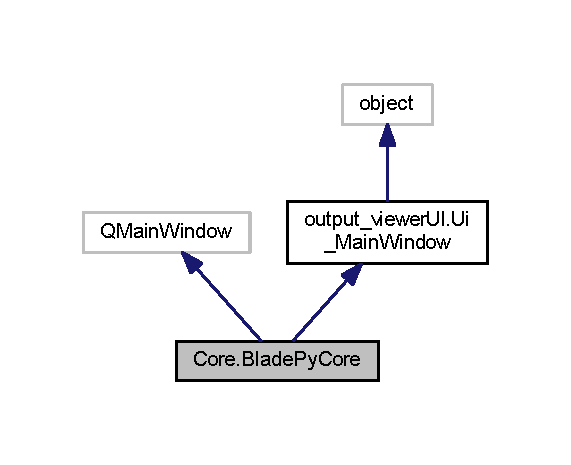
\includegraphics[width=274pt]{class_core_1_1_blade_py_core__inherit__graph}
\end{center}
\end{figure}
\subsection*{Public Member Functions}
\begin{DoxyCompactItemize}
\item 
def \hyperlink{class_core_1_1_blade_py_core_a10b91a0caafffe00be0f4fa9c7a022dc}{\+\_\+\+\_\+init\+\_\+\+\_\+} (self, parent=None)
\item 
def \hyperlink{class_core_1_1_blade_py_core_ade955a1fc8334b12726d9f462ed25c62}{toolbar\+View\+Button\+Pressed\+Group} (self, pressed\+\_\+btn)
\begin{DoxyCompactList}\small\item\em Method group that wrap all functions for shape viewing toolbar. \end{DoxyCompactList}\item 
def \hyperlink{class_core_1_1_blade_py_core_ab5cf733dc40f2b17761056148fd51263}{toolbar\+File\+Button\+Pressed\+Group} (self, pressed\+\_\+btn)
\begin{DoxyCompactList}\small\item\em Method group that wrap all functions for \char`\"{}file\char`\"{} toolbar. \end{DoxyCompactList}\item 
def \hyperlink{class_core_1_1_blade_py_core_aabfc46144de45158b8d9c8952cfa1a7d}{toolbar\+Tecplot\+Button\+Pressed\+Group} (self, pressed\+\_\+btn)
\begin{DoxyCompactList}\small\item\em Method group that wrap all functions for tecplot options in toolbar. \end{DoxyCompactList}\item 
def \hyperlink{class_core_1_1_blade_py_core_abe6ec5c591c19b280f2e24bb198a1d6b}{toolbar\+Settings\+Button\+Pressed\+Group} (self, pressed\+\_\+btn)
\begin{DoxyCompactList}\small\item\em Method group that wrap all functions for \char`\"{}settings\char`\"{} toolbar. \end{DoxyCompactList}\item 
def \hyperlink{class_core_1_1_blade_py_core_aedcbcf23c32b9661d48f28e11c0c7172}{menu\+File\+Button\+Pressed\+Group} (self, pressed\+\_\+btn)
\begin{DoxyCompactList}\small\item\em Method group that wrap only exit function for \char`\"{}file\char`\"{} menu. \end{DoxyCompactList}\item 
def \hyperlink{class_core_1_1_blade_py_core_ac45b825bd62e01689fb2987a0a2d850a}{open\+Case} (self)
\begin{DoxyCompactList}\small\item\em Opens a case previously generated by Blade\+Pro. \end{DoxyCompactList}\item 
def \hyperlink{class_core_1_1_blade_py_core_a1a62f9b5b8f5929bdb6f0a8c27049d9e}{add\+Case} (self)
\begin{DoxyCompactList}\small\item\em Method that adds a Case in Output Viewer. \end{DoxyCompactList}\item 
def \hyperlink{class_core_1_1_blade_py_core_a305ea5ff4997029c7a54a4550a23eba8}{delete\+Case} (self)
\begin{DoxyCompactList}\small\item\em Method for deleting loaded cases in model tree view. \end{DoxyCompactList}\item 
def \hyperlink{class_core_1_1_blade_py_core_a2c818d907d8c5797873e1a7ad54c7d13}{set\+Zoom\+Factor} (self)
\begin{DoxyCompactList}\small\item\em Sets the zoom factor for shape viewing. \end{DoxyCompactList}\end{DoxyCompactItemize}
\subsection*{Public Attributes}
\begin{DoxyCompactItemize}
\item 
\hyperlink{class_core_1_1_blade_py_core_a84a62c3017515ec840e35dbbe8ccbf21}{current\+\_\+h\+\_\+ais\+\_\+shape}
\begin{DoxyCompactList}\small\item\em This attribute is used all around the code and represents the \char`\"{}working\char`\"{} shape. \end{DoxyCompactList}\item 
\hyperlink{class_core_1_1_blade_py_core_a76f4a1191b8d68c0ed9d9f3e1e6756d8}{case\+\_\+node}
\begin{DoxyCompactList}\small\item\em This attribute is the entity that represents the unity of a case. \end{DoxyCompactList}\item 
\hyperlink{class_core_1_1_blade_py_core_a43d75821c1883b1b972c8e0ef9922b4a}{previous\+\_\+case\+\_\+node}
\item 
\hyperlink{class_core_1_1_blade_py_core_a84adec7b4b982bce58747d39e098236f}{selection\+Mode}
\begin{DoxyCompactList}\small\item\em This attribute is one that is used by the program to tell whether the user is managing a shape or sub-\/shape. \end{DoxyCompactList}\item 
\hyperlink{class_core_1_1_blade_py_core_a819ef9e1cd2f233d92a5379532060bd0}{master\+\_\+shape\+\_\+list}
\begin{DoxyCompactList}\small\item\em This attribute is a list that contains all shapes loaded in the program. \end{DoxyCompactList}\item 
\hyperlink{class_core_1_1_blade_py_core_a96038d8a4727208ba2e9cd359bcd4781}{list\+\_\+settings}
\item 
\hyperlink{class_core_1_1_blade_py_core_abfb58254f95f980e2821bac01114cd40}{Preferences\+Manager}
\item 
\hyperlink{class_core_1_1_blade_py_core_a1e75ee619926a396b584090b2707b1ca}{Shape\+Manager}
\begin{DoxyCompactList}\small\item\em This attribute is an object used for managing shape properties. \end{DoxyCompactList}\item 
\hyperlink{class_core_1_1_blade_py_core_a3cbd742c4a4a706d44d5265e19b25aaa}{root\+Node}
\begin{DoxyCompactList}\small\item\em This attribute is the object node of all case nodes. \end{DoxyCompactList}\item 
\hyperlink{class_core_1_1_blade_py_core_ac74bebda7bd9e99df8e5d26c0b61e0bb}{model}
\begin{DoxyCompactList}\small\item\em This attribute is the model object that is the intermediary between the tree view and the case node. \end{DoxyCompactList}\item 
\hyperlink{class_core_1_1_blade_py_core_ab277fbfb8af6b2ef9aff8d06c9f5cc82}{canva}
\begin{DoxyCompactList}\small\item\em This is the object of the Qt\+Viewer of Python\+O\+CC. \end{DoxyCompactList}\item 
\hyperlink{class_core_1_1_blade_py_core_abe828f3ea500c70a4abe0f376b6d8dc4}{display}
\begin{DoxyCompactList}\small\item\em This attribute is O\+C\+C\+Viewer.\+Viewer3d(self.\+Get\+Handle()), used to manage the 3D graphics. \end{DoxyCompactList}\item 
\hyperlink{class_core_1_1_blade_py_core_a8d53bb9fe024d3235652a6233d0d61a8}{DC}
\item 
\hyperlink{class_core_1_1_blade_py_core_a62af2479e8c1b0d3405a6122ea2be116}{D\+C\+\_\+\+H\+LR}
\item 
\hyperlink{class_core_1_1_blade_py_core_a04f16a810669c721b389767d47c08c8f}{Tecplot\+Viewer\+Widget}
\item 
\hyperlink{class_core_1_1_blade_py_core_a4ead2c1cc874da56fad290cca0630fc0}{Input\+Writer\+Widget}
\item 
\hyperlink{class_core_1_1_blade_py_core_af0ce94ff8ed058ada4057b3062de1d0d}{first\+\_\+default}
\item 
\hyperlink{class_core_1_1_blade_py_core_a74bd4997b68dd3f273e5eb6cbbbac70a}{default\+\_\+shape\+\_\+color}
\item 
\hyperlink{class_core_1_1_blade_py_core_aafff31611ea2a5eb584f2550607e3e23}{default\+\_\+shape\+\_\+factor}
\item 
\hyperlink{class_core_1_1_blade_py_core_a26accbeb5266ec3f792c86cf8643f696}{default\+\_\+shape\+\_\+transparency}
\end{DoxyCompactItemize}


\subsection{Detailed Description}
This is the key Class that wraps all the other packages and modules of Blade\+Py. 

This class is responsible for adding functions to the inherited \hyperlink{classoutput__viewer_u_i_1_1_ui___main_window}{output\+\_\+viewer\+U\+I.\+Ui\+\_\+\+Main\+Window} function-\/less layout created in Qt Designer.

This class has methods for managing the display of the outputs generated by Blade\+Pro. It has the methods for loading any case that was previously generated by Blade\+Pro. It can also retrieve the outputs of Blade\+Pro as soon as they were created if desired in the \hyperlink{classbladepro__modules_1_1inputfile__writer_1_1_input_writer_window}{bladepro\+\_\+modules.\+inputfile\+\_\+writer.\+Input\+Writer\+Window}

Classes of other Blade\+Py modules of objects created by \hyperlink{class_core_1_1_blade_py_core}{Blade\+Py\+Core} (composition association)

For output display\+: \begin{DoxyItemize}
\item {\ttfamily \hyperlink{classbladepro__modules_1_1inputfile__writer_1_1_input_writer_window}{bladepro\+\_\+modules.\+inputfile\+\_\+writer.\+Input\+Writer\+Window}} -\/ For writing inputfiles and Blade\+Pro communication \item {\ttfamily \hyperlink{classtecplot__modules_1_1tecplot__display_1_1_tec_plot_window}{tecplot\+\_\+modules.\+tecplot\+\_\+display.\+Tec\+Plot\+Window}} -\/ For displaying tecplot graphics \item {\ttfamily \hyperlink{classocc__modules_1_1qt__display_1_1custom_qt_viewer3d}{occ\+\_\+modules.\+qt\+\_\+display.\+custom\+Qt\+Viewer3d}} -\/ For creating a customized viewer for Open\+Cascade \item {\ttfamily occ\+\_\+modules.\+shape\+\_\+properties.\+custom\+Qt\+Viewer3d} -\/ For creating a customized viewer for Open\+Cascade\end{DoxyItemize}
For data management\+: \begin{DoxyItemize}
\item {\ttfamily \hyperlink{classdata__structure_1_1case__model_1_1_case_model}{data\+\_\+structure.\+case\+\_\+model.\+Case\+Model}} -\/ For creating a model for Tree\+View list \item {\ttfamily \hyperlink{classdata__structure_1_1case__node_1_1_case_node}{data\+\_\+structure.\+case\+\_\+node.\+Case\+Node}} -\/ For creating a information center for cases\end{DoxyItemize}
For user settings\+: \begin{DoxyItemize}
\item {\ttfamily \hyperlink{classsettings_1_1preferences_1_1_preferences_blade_py}{settings.\+preferences.\+Preferences\+Blade\+Py}} -\/ For managing User Preferences \end{DoxyItemize}


\subsection{Constructor \& Destructor Documentation}
\hypertarget{class_core_1_1_blade_py_core_a10b91a0caafffe00be0f4fa9c7a022dc}{}\label{class_core_1_1_blade_py_core_a10b91a0caafffe00be0f4fa9c7a022dc} 
\index{Core\+::\+Blade\+Py\+Core@{Core\+::\+Blade\+Py\+Core}!\+\_\+\+\_\+init\+\_\+\+\_\+@{\+\_\+\+\_\+init\+\_\+\+\_\+}}
\index{\+\_\+\+\_\+init\+\_\+\+\_\+@{\+\_\+\+\_\+init\+\_\+\+\_\+}!Core\+::\+Blade\+Py\+Core@{Core\+::\+Blade\+Py\+Core}}
\subsubsection{\texorpdfstring{\+\_\+\+\_\+init\+\_\+\+\_\+()}{\_\_init\_\_()}}
{\footnotesize\ttfamily def Core.\+Blade\+Py\+Core.\+\_\+\+\_\+init\+\_\+\+\_\+ (\begin{DoxyParamCaption}\item[{}]{self,  }\item[{}]{parent = {\ttfamily None} }\end{DoxyParamCaption})}



\subsection{Member Function Documentation}
\hypertarget{class_core_1_1_blade_py_core_a1a62f9b5b8f5929bdb6f0a8c27049d9e}{}\label{class_core_1_1_blade_py_core_a1a62f9b5b8f5929bdb6f0a8c27049d9e} 
\index{Core\+::\+Blade\+Py\+Core@{Core\+::\+Blade\+Py\+Core}!add\+Case@{add\+Case}}
\index{add\+Case@{add\+Case}!Core\+::\+Blade\+Py\+Core@{Core\+::\+Blade\+Py\+Core}}
\subsubsection{\texorpdfstring{add\+Case()}{addCase()}}
{\footnotesize\ttfamily def Core.\+Blade\+Py\+Core.\+add\+Case (\begin{DoxyParamCaption}\item[{}]{self,  }\item[{}]{object }\end{DoxyParamCaption})}



Method that adds a Case in Output Viewer. 

This will be triggered by the Output Viewer when opening an existing case or when Run Blade\+Pro button is clicked in in the Input Writer G\+UI. This method will read files related to the working case. Currently, the add\+Case method supports three outputs from Blade\+Pro.

\begin{DoxyItemize}
\item I\+GS 3D Curves; \item I\+GS Surfaces; \item Tecplots 2D.\end{DoxyItemize}
\begin{DoxyReturn}{Returns}
None 
\end{DoxyReturn}
\hypertarget{class_core_1_1_blade_py_core_a305ea5ff4997029c7a54a4550a23eba8}{}\label{class_core_1_1_blade_py_core_a305ea5ff4997029c7a54a4550a23eba8} 
\index{Core\+::\+Blade\+Py\+Core@{Core\+::\+Blade\+Py\+Core}!delete\+Case@{delete\+Case}}
\index{delete\+Case@{delete\+Case}!Core\+::\+Blade\+Py\+Core@{Core\+::\+Blade\+Py\+Core}}
\subsubsection{\texorpdfstring{delete\+Case()}{deleteCase()}}
{\footnotesize\ttfamily def Core.\+Blade\+Py\+Core.\+delete\+Case (\begin{DoxyParamCaption}\item[{}]{self }\end{DoxyParamCaption})}



Method for deleting loaded cases in model tree view. 

It deletes the interactive A\+IS Shape, the tecplots from Display and data structure.

\begin{DoxyReturn}{Returns}
None 
\end{DoxyReturn}
\hypertarget{class_core_1_1_blade_py_core_aedcbcf23c32b9661d48f28e11c0c7172}{}\label{class_core_1_1_blade_py_core_aedcbcf23c32b9661d48f28e11c0c7172} 
\index{Core\+::\+Blade\+Py\+Core@{Core\+::\+Blade\+Py\+Core}!menu\+File\+Button\+Pressed\+Group@{menu\+File\+Button\+Pressed\+Group}}
\index{menu\+File\+Button\+Pressed\+Group@{menu\+File\+Button\+Pressed\+Group}!Core\+::\+Blade\+Py\+Core@{Core\+::\+Blade\+Py\+Core}}
\subsubsection{\texorpdfstring{menu\+File\+Button\+Pressed\+Group()}{menuFileButtonPressedGroup()}}
{\footnotesize\ttfamily def Core.\+Blade\+Py\+Core.\+menu\+File\+Button\+Pressed\+Group (\begin{DoxyParamCaption}\item[{}]{self,  }\item[{}]{pressed\+\_\+btn }\end{DoxyParamCaption})}



Method group that wrap only exit function for \char`\"{}file\char`\"{} menu. 


\begin{DoxyParams}{Parameters}
{\em pressed\+\_\+btn} & \mbox{[}Qt\+Gui.\+Q\+Action\mbox{]} Signal emitted by button clicked on ui\+\_\+file\+\_\+menur \\
\hline
\end{DoxyParams}
\begin{DoxyReturn}{Returns}
None 
\end{DoxyReturn}
\hypertarget{class_core_1_1_blade_py_core_ac45b825bd62e01689fb2987a0a2d850a}{}\label{class_core_1_1_blade_py_core_ac45b825bd62e01689fb2987a0a2d850a} 
\index{Core\+::\+Blade\+Py\+Core@{Core\+::\+Blade\+Py\+Core}!open\+Case@{open\+Case}}
\index{open\+Case@{open\+Case}!Core\+::\+Blade\+Py\+Core@{Core\+::\+Blade\+Py\+Core}}
\subsubsection{\texorpdfstring{open\+Case()}{openCase()}}
{\footnotesize\ttfamily def Core.\+Blade\+Py\+Core.\+open\+Case (\begin{DoxyParamCaption}\item[{}]{self }\end{DoxyParamCaption})}



Opens a case previously generated by Blade\+Pro. 

Any file generated by Blade\+Pro can be used to open case. The program will look for other files with the same case name in the same folder.

\begin{DoxyReturn}{Returns}
None 
\end{DoxyReturn}
\hypertarget{class_core_1_1_blade_py_core_a2c818d907d8c5797873e1a7ad54c7d13}{}\label{class_core_1_1_blade_py_core_a2c818d907d8c5797873e1a7ad54c7d13} 
\index{Core\+::\+Blade\+Py\+Core@{Core\+::\+Blade\+Py\+Core}!set\+Zoom\+Factor@{set\+Zoom\+Factor}}
\index{set\+Zoom\+Factor@{set\+Zoom\+Factor}!Core\+::\+Blade\+Py\+Core@{Core\+::\+Blade\+Py\+Core}}
\subsubsection{\texorpdfstring{set\+Zoom\+Factor()}{setZoomFactor()}}
{\footnotesize\ttfamily def Core.\+Blade\+Py\+Core.\+set\+Zoom\+Factor (\begin{DoxyParamCaption}\item[{}]{self }\end{DoxyParamCaption})}



Sets the zoom factor for shape viewing. 

\begin{DoxyReturn}{Returns}
None 
\end{DoxyReturn}
\hypertarget{class_core_1_1_blade_py_core_ab5cf733dc40f2b17761056148fd51263}{}\label{class_core_1_1_blade_py_core_ab5cf733dc40f2b17761056148fd51263} 
\index{Core\+::\+Blade\+Py\+Core@{Core\+::\+Blade\+Py\+Core}!toolbar\+File\+Button\+Pressed\+Group@{toolbar\+File\+Button\+Pressed\+Group}}
\index{toolbar\+File\+Button\+Pressed\+Group@{toolbar\+File\+Button\+Pressed\+Group}!Core\+::\+Blade\+Py\+Core@{Core\+::\+Blade\+Py\+Core}}
\subsubsection{\texorpdfstring{toolbar\+File\+Button\+Pressed\+Group()}{toolbarFileButtonPressedGroup()}}
{\footnotesize\ttfamily def Core.\+Blade\+Py\+Core.\+toolbar\+File\+Button\+Pressed\+Group (\begin{DoxyParamCaption}\item[{}]{self,  }\item[{}]{pressed\+\_\+btn }\end{DoxyParamCaption})}



Method group that wrap all functions for \char`\"{}file\char`\"{} toolbar. 


\begin{DoxyParams}{Parameters}
{\em pressed\+\_\+btn} & \mbox{[}Qt\+Gui.\+Q\+Action\mbox{]} Signal emitted by button clicked on ui\+\_\+file\+\_\+toolbar \\
\hline
\end{DoxyParams}
\begin{DoxyReturn}{Returns}
None 
\end{DoxyReturn}
\hypertarget{class_core_1_1_blade_py_core_abe6ec5c591c19b280f2e24bb198a1d6b}{}\label{class_core_1_1_blade_py_core_abe6ec5c591c19b280f2e24bb198a1d6b} 
\index{Core\+::\+Blade\+Py\+Core@{Core\+::\+Blade\+Py\+Core}!toolbar\+Settings\+Button\+Pressed\+Group@{toolbar\+Settings\+Button\+Pressed\+Group}}
\index{toolbar\+Settings\+Button\+Pressed\+Group@{toolbar\+Settings\+Button\+Pressed\+Group}!Core\+::\+Blade\+Py\+Core@{Core\+::\+Blade\+Py\+Core}}
\subsubsection{\texorpdfstring{toolbar\+Settings\+Button\+Pressed\+Group()}{toolbarSettingsButtonPressedGroup()}}
{\footnotesize\ttfamily def Core.\+Blade\+Py\+Core.\+toolbar\+Settings\+Button\+Pressed\+Group (\begin{DoxyParamCaption}\item[{}]{self,  }\item[{}]{pressed\+\_\+btn }\end{DoxyParamCaption})}



Method group that wrap all functions for \char`\"{}settings\char`\"{} toolbar. 


\begin{DoxyParams}{Parameters}
{\em pressed\+\_\+btn} & \mbox{[}Qt\+Gui.\+Q\+Action\mbox{]} Signal emitted by button clicked on ui\+\_\+file\+\_\+toolbar \\
\hline
\end{DoxyParams}
\begin{DoxyReturn}{Returns}
None 
\end{DoxyReturn}
\hypertarget{class_core_1_1_blade_py_core_aabfc46144de45158b8d9c8952cfa1a7d}{}\label{class_core_1_1_blade_py_core_aabfc46144de45158b8d9c8952cfa1a7d} 
\index{Core\+::\+Blade\+Py\+Core@{Core\+::\+Blade\+Py\+Core}!toolbar\+Tecplot\+Button\+Pressed\+Group@{toolbar\+Tecplot\+Button\+Pressed\+Group}}
\index{toolbar\+Tecplot\+Button\+Pressed\+Group@{toolbar\+Tecplot\+Button\+Pressed\+Group}!Core\+::\+Blade\+Py\+Core@{Core\+::\+Blade\+Py\+Core}}
\subsubsection{\texorpdfstring{toolbar\+Tecplot\+Button\+Pressed\+Group()}{toolbarTecplotButtonPressedGroup()}}
{\footnotesize\ttfamily def Core.\+Blade\+Py\+Core.\+toolbar\+Tecplot\+Button\+Pressed\+Group (\begin{DoxyParamCaption}\item[{}]{self,  }\item[{}]{pressed\+\_\+btn }\end{DoxyParamCaption})}



Method group that wrap all functions for tecplot options in toolbar. 


\begin{DoxyParams}{Parameters}
{\em pressed\+\_\+btn} & \mbox{[}Qt\+Gui.\+Q\+Action\mbox{]} Signal emitted by button clicked on ui\+\_\+tecplot\+\_\+toolbar \\
\hline
\end{DoxyParams}
\begin{DoxyReturn}{Returns}
None 
\end{DoxyReturn}
\hypertarget{class_core_1_1_blade_py_core_ade955a1fc8334b12726d9f462ed25c62}{}\label{class_core_1_1_blade_py_core_ade955a1fc8334b12726d9f462ed25c62} 
\index{Core\+::\+Blade\+Py\+Core@{Core\+::\+Blade\+Py\+Core}!toolbar\+View\+Button\+Pressed\+Group@{toolbar\+View\+Button\+Pressed\+Group}}
\index{toolbar\+View\+Button\+Pressed\+Group@{toolbar\+View\+Button\+Pressed\+Group}!Core\+::\+Blade\+Py\+Core@{Core\+::\+Blade\+Py\+Core}}
\subsubsection{\texorpdfstring{toolbar\+View\+Button\+Pressed\+Group()}{toolbarViewButtonPressedGroup()}}
{\footnotesize\ttfamily def Core.\+Blade\+Py\+Core.\+toolbar\+View\+Button\+Pressed\+Group (\begin{DoxyParamCaption}\item[{}]{self,  }\item[{}]{pressed\+\_\+btn }\end{DoxyParamCaption})}



Method group that wrap all functions for shape viewing toolbar. 


\begin{DoxyParams}{Parameters}
{\em pressed\+\_\+btn} & \mbox{[}Qt\+Gui.\+Q\+Action\mbox{]} Signal emitted by button clicked on ui\+\_\+view\+\_\+toolbar \\
\hline
\end{DoxyParams}
\begin{DoxyReturn}{Returns}
None 
\end{DoxyReturn}


\subsection{Member Data Documentation}
\hypertarget{class_core_1_1_blade_py_core_ab277fbfb8af6b2ef9aff8d06c9f5cc82}{}\label{class_core_1_1_blade_py_core_ab277fbfb8af6b2ef9aff8d06c9f5cc82} 
\index{Core\+::\+Blade\+Py\+Core@{Core\+::\+Blade\+Py\+Core}!canva@{canva}}
\index{canva@{canva}!Core\+::\+Blade\+Py\+Core@{Core\+::\+Blade\+Py\+Core}}
\subsubsection{\texorpdfstring{canva}{canva}}
{\footnotesize\ttfamily Core.\+Blade\+Py\+Core.\+canva}



This is the object of the Qt\+Viewer of Python\+O\+CC. 

\hypertarget{class_core_1_1_blade_py_core_a76f4a1191b8d68c0ed9d9f3e1e6756d8}{}\label{class_core_1_1_blade_py_core_a76f4a1191b8d68c0ed9d9f3e1e6756d8} 
\index{Core\+::\+Blade\+Py\+Core@{Core\+::\+Blade\+Py\+Core}!case\+\_\+node@{case\+\_\+node}}
\index{case\+\_\+node@{case\+\_\+node}!Core\+::\+Blade\+Py\+Core@{Core\+::\+Blade\+Py\+Core}}
\subsubsection{\texorpdfstring{case\+\_\+node}{case\_node}}
{\footnotesize\ttfamily Core.\+Blade\+Py\+Core.\+case\+\_\+node}



This attribute is the entity that represents the unity of a case. 

\hypertarget{class_core_1_1_blade_py_core_a84a62c3017515ec840e35dbbe8ccbf21}{}\label{class_core_1_1_blade_py_core_a84a62c3017515ec840e35dbbe8ccbf21} 
\index{Core\+::\+Blade\+Py\+Core@{Core\+::\+Blade\+Py\+Core}!current\+\_\+h\+\_\+ais\+\_\+shape@{current\+\_\+h\+\_\+ais\+\_\+shape}}
\index{current\+\_\+h\+\_\+ais\+\_\+shape@{current\+\_\+h\+\_\+ais\+\_\+shape}!Core\+::\+Blade\+Py\+Core@{Core\+::\+Blade\+Py\+Core}}
\subsubsection{\texorpdfstring{current\+\_\+h\+\_\+ais\+\_\+shape}{current\_h\_ais\_shape}}
{\footnotesize\ttfamily Core.\+Blade\+Py\+Core.\+current\+\_\+h\+\_\+ais\+\_\+shape}



This attribute is used all around the code and represents the \char`\"{}working\char`\"{} shape. 

\hypertarget{class_core_1_1_blade_py_core_a8d53bb9fe024d3235652a6233d0d61a8}{}\label{class_core_1_1_blade_py_core_a8d53bb9fe024d3235652a6233d0d61a8} 
\index{Core\+::\+Blade\+Py\+Core@{Core\+::\+Blade\+Py\+Core}!DC@{DC}}
\index{DC@{DC}!Core\+::\+Blade\+Py\+Core@{Core\+::\+Blade\+Py\+Core}}
\subsubsection{\texorpdfstring{DC}{DC}}
{\footnotesize\ttfamily Core.\+Blade\+Py\+Core.\+DC}

\hypertarget{class_core_1_1_blade_py_core_a62af2479e8c1b0d3405a6122ea2be116}{}\label{class_core_1_1_blade_py_core_a62af2479e8c1b0d3405a6122ea2be116} 
\index{Core\+::\+Blade\+Py\+Core@{Core\+::\+Blade\+Py\+Core}!D\+C\+\_\+\+H\+LR@{D\+C\+\_\+\+H\+LR}}
\index{D\+C\+\_\+\+H\+LR@{D\+C\+\_\+\+H\+LR}!Core\+::\+Blade\+Py\+Core@{Core\+::\+Blade\+Py\+Core}}
\subsubsection{\texorpdfstring{D\+C\+\_\+\+H\+LR}{DC\_HLR}}
{\footnotesize\ttfamily Core.\+Blade\+Py\+Core.\+D\+C\+\_\+\+H\+LR}

\hypertarget{class_core_1_1_blade_py_core_a74bd4997b68dd3f273e5eb6cbbbac70a}{}\label{class_core_1_1_blade_py_core_a74bd4997b68dd3f273e5eb6cbbbac70a} 
\index{Core\+::\+Blade\+Py\+Core@{Core\+::\+Blade\+Py\+Core}!default\+\_\+shape\+\_\+color@{default\+\_\+shape\+\_\+color}}
\index{default\+\_\+shape\+\_\+color@{default\+\_\+shape\+\_\+color}!Core\+::\+Blade\+Py\+Core@{Core\+::\+Blade\+Py\+Core}}
\subsubsection{\texorpdfstring{default\+\_\+shape\+\_\+color}{default\_shape\_color}}
{\footnotesize\ttfamily Core.\+Blade\+Py\+Core.\+default\+\_\+shape\+\_\+color}

\hypertarget{class_core_1_1_blade_py_core_aafff31611ea2a5eb584f2550607e3e23}{}\label{class_core_1_1_blade_py_core_aafff31611ea2a5eb584f2550607e3e23} 
\index{Core\+::\+Blade\+Py\+Core@{Core\+::\+Blade\+Py\+Core}!default\+\_\+shape\+\_\+factor@{default\+\_\+shape\+\_\+factor}}
\index{default\+\_\+shape\+\_\+factor@{default\+\_\+shape\+\_\+factor}!Core\+::\+Blade\+Py\+Core@{Core\+::\+Blade\+Py\+Core}}
\subsubsection{\texorpdfstring{default\+\_\+shape\+\_\+factor}{default\_shape\_factor}}
{\footnotesize\ttfamily Core.\+Blade\+Py\+Core.\+default\+\_\+shape\+\_\+factor}

\hypertarget{class_core_1_1_blade_py_core_a26accbeb5266ec3f792c86cf8643f696}{}\label{class_core_1_1_blade_py_core_a26accbeb5266ec3f792c86cf8643f696} 
\index{Core\+::\+Blade\+Py\+Core@{Core\+::\+Blade\+Py\+Core}!default\+\_\+shape\+\_\+transparency@{default\+\_\+shape\+\_\+transparency}}
\index{default\+\_\+shape\+\_\+transparency@{default\+\_\+shape\+\_\+transparency}!Core\+::\+Blade\+Py\+Core@{Core\+::\+Blade\+Py\+Core}}
\subsubsection{\texorpdfstring{default\+\_\+shape\+\_\+transparency}{default\_shape\_transparency}}
{\footnotesize\ttfamily Core.\+Blade\+Py\+Core.\+default\+\_\+shape\+\_\+transparency}

\hypertarget{class_core_1_1_blade_py_core_abe828f3ea500c70a4abe0f376b6d8dc4}{}\label{class_core_1_1_blade_py_core_abe828f3ea500c70a4abe0f376b6d8dc4} 
\index{Core\+::\+Blade\+Py\+Core@{Core\+::\+Blade\+Py\+Core}!display@{display}}
\index{display@{display}!Core\+::\+Blade\+Py\+Core@{Core\+::\+Blade\+Py\+Core}}
\subsubsection{\texorpdfstring{display}{display}}
{\footnotesize\ttfamily Core.\+Blade\+Py\+Core.\+display}



This attribute is O\+C\+C\+Viewer.\+Viewer3d(self.\+Get\+Handle()), used to manage the 3D graphics. 

\hypertarget{class_core_1_1_blade_py_core_af0ce94ff8ed058ada4057b3062de1d0d}{}\label{class_core_1_1_blade_py_core_af0ce94ff8ed058ada4057b3062de1d0d} 
\index{Core\+::\+Blade\+Py\+Core@{Core\+::\+Blade\+Py\+Core}!first\+\_\+default@{first\+\_\+default}}
\index{first\+\_\+default@{first\+\_\+default}!Core\+::\+Blade\+Py\+Core@{Core\+::\+Blade\+Py\+Core}}
\subsubsection{\texorpdfstring{first\+\_\+default}{first\_default}}
{\footnotesize\ttfamily Core.\+Blade\+Py\+Core.\+first\+\_\+default}

\hypertarget{class_core_1_1_blade_py_core_a4ead2c1cc874da56fad290cca0630fc0}{}\label{class_core_1_1_blade_py_core_a4ead2c1cc874da56fad290cca0630fc0} 
\index{Core\+::\+Blade\+Py\+Core@{Core\+::\+Blade\+Py\+Core}!Input\+Writer\+Widget@{Input\+Writer\+Widget}}
\index{Input\+Writer\+Widget@{Input\+Writer\+Widget}!Core\+::\+Blade\+Py\+Core@{Core\+::\+Blade\+Py\+Core}}
\subsubsection{\texorpdfstring{Input\+Writer\+Widget}{InputWriterWidget}}
{\footnotesize\ttfamily Core.\+Blade\+Py\+Core.\+Input\+Writer\+Widget}

\hypertarget{class_core_1_1_blade_py_core_a96038d8a4727208ba2e9cd359bcd4781}{}\label{class_core_1_1_blade_py_core_a96038d8a4727208ba2e9cd359bcd4781} 
\index{Core\+::\+Blade\+Py\+Core@{Core\+::\+Blade\+Py\+Core}!list\+\_\+settings@{list\+\_\+settings}}
\index{list\+\_\+settings@{list\+\_\+settings}!Core\+::\+Blade\+Py\+Core@{Core\+::\+Blade\+Py\+Core}}
\subsubsection{\texorpdfstring{list\+\_\+settings}{list\_settings}}
{\footnotesize\ttfamily Core.\+Blade\+Py\+Core.\+list\+\_\+settings}

\hypertarget{class_core_1_1_blade_py_core_a819ef9e1cd2f233d92a5379532060bd0}{}\label{class_core_1_1_blade_py_core_a819ef9e1cd2f233d92a5379532060bd0} 
\index{Core\+::\+Blade\+Py\+Core@{Core\+::\+Blade\+Py\+Core}!master\+\_\+shape\+\_\+list@{master\+\_\+shape\+\_\+list}}
\index{master\+\_\+shape\+\_\+list@{master\+\_\+shape\+\_\+list}!Core\+::\+Blade\+Py\+Core@{Core\+::\+Blade\+Py\+Core}}
\subsubsection{\texorpdfstring{master\+\_\+shape\+\_\+list}{master\_shape\_list}}
{\footnotesize\ttfamily Core.\+Blade\+Py\+Core.\+master\+\_\+shape\+\_\+list}



This attribute is a list that contains all shapes loaded in the program. 

\hypertarget{class_core_1_1_blade_py_core_ac74bebda7bd9e99df8e5d26c0b61e0bb}{}\label{class_core_1_1_blade_py_core_ac74bebda7bd9e99df8e5d26c0b61e0bb} 
\index{Core\+::\+Blade\+Py\+Core@{Core\+::\+Blade\+Py\+Core}!model@{model}}
\index{model@{model}!Core\+::\+Blade\+Py\+Core@{Core\+::\+Blade\+Py\+Core}}
\subsubsection{\texorpdfstring{model}{model}}
{\footnotesize\ttfamily Core.\+Blade\+Py\+Core.\+model}



This attribute is the model object that is the intermediary between the tree view and the case node. 

\hypertarget{class_core_1_1_blade_py_core_abfb58254f95f980e2821bac01114cd40}{}\label{class_core_1_1_blade_py_core_abfb58254f95f980e2821bac01114cd40} 
\index{Core\+::\+Blade\+Py\+Core@{Core\+::\+Blade\+Py\+Core}!Preferences\+Manager@{Preferences\+Manager}}
\index{Preferences\+Manager@{Preferences\+Manager}!Core\+::\+Blade\+Py\+Core@{Core\+::\+Blade\+Py\+Core}}
\subsubsection{\texorpdfstring{Preferences\+Manager}{PreferencesManager}}
{\footnotesize\ttfamily Core.\+Blade\+Py\+Core.\+Preferences\+Manager}

\hypertarget{class_core_1_1_blade_py_core_a43d75821c1883b1b972c8e0ef9922b4a}{}\label{class_core_1_1_blade_py_core_a43d75821c1883b1b972c8e0ef9922b4a} 
\index{Core\+::\+Blade\+Py\+Core@{Core\+::\+Blade\+Py\+Core}!previous\+\_\+case\+\_\+node@{previous\+\_\+case\+\_\+node}}
\index{previous\+\_\+case\+\_\+node@{previous\+\_\+case\+\_\+node}!Core\+::\+Blade\+Py\+Core@{Core\+::\+Blade\+Py\+Core}}
\subsubsection{\texorpdfstring{previous\+\_\+case\+\_\+node}{previous\_case\_node}}
{\footnotesize\ttfamily Core.\+Blade\+Py\+Core.\+previous\+\_\+case\+\_\+node}

\hypertarget{class_core_1_1_blade_py_core_a3cbd742c4a4a706d44d5265e19b25aaa}{}\label{class_core_1_1_blade_py_core_a3cbd742c4a4a706d44d5265e19b25aaa} 
\index{Core\+::\+Blade\+Py\+Core@{Core\+::\+Blade\+Py\+Core}!root\+Node@{root\+Node}}
\index{root\+Node@{root\+Node}!Core\+::\+Blade\+Py\+Core@{Core\+::\+Blade\+Py\+Core}}
\subsubsection{\texorpdfstring{root\+Node}{rootNode}}
{\footnotesize\ttfamily Core.\+Blade\+Py\+Core.\+root\+Node}



This attribute is the object node of all case nodes. 

\hypertarget{class_core_1_1_blade_py_core_a84adec7b4b982bce58747d39e098236f}{}\label{class_core_1_1_blade_py_core_a84adec7b4b982bce58747d39e098236f} 
\index{Core\+::\+Blade\+Py\+Core@{Core\+::\+Blade\+Py\+Core}!selection\+Mode@{selection\+Mode}}
\index{selection\+Mode@{selection\+Mode}!Core\+::\+Blade\+Py\+Core@{Core\+::\+Blade\+Py\+Core}}
\subsubsection{\texorpdfstring{selection\+Mode}{selectionMode}}
{\footnotesize\ttfamily Core.\+Blade\+Py\+Core.\+selection\+Mode}



This attribute is one that is used by the program to tell whether the user is managing a shape or sub-\/shape. 

\hypertarget{class_core_1_1_blade_py_core_a1e75ee619926a396b584090b2707b1ca}{}\label{class_core_1_1_blade_py_core_a1e75ee619926a396b584090b2707b1ca} 
\index{Core\+::\+Blade\+Py\+Core@{Core\+::\+Blade\+Py\+Core}!Shape\+Manager@{Shape\+Manager}}
\index{Shape\+Manager@{Shape\+Manager}!Core\+::\+Blade\+Py\+Core@{Core\+::\+Blade\+Py\+Core}}
\subsubsection{\texorpdfstring{Shape\+Manager}{ShapeManager}}
{\footnotesize\ttfamily Core.\+Blade\+Py\+Core.\+Shape\+Manager}



This attribute is an object used for managing shape properties. 

\hypertarget{class_core_1_1_blade_py_core_a04f16a810669c721b389767d47c08c8f}{}\label{class_core_1_1_blade_py_core_a04f16a810669c721b389767d47c08c8f} 
\index{Core\+::\+Blade\+Py\+Core@{Core\+::\+Blade\+Py\+Core}!Tecplot\+Viewer\+Widget@{Tecplot\+Viewer\+Widget}}
\index{Tecplot\+Viewer\+Widget@{Tecplot\+Viewer\+Widget}!Core\+::\+Blade\+Py\+Core@{Core\+::\+Blade\+Py\+Core}}
\subsubsection{\texorpdfstring{Tecplot\+Viewer\+Widget}{TecplotViewerWidget}}
{\footnotesize\ttfamily Core.\+Blade\+Py\+Core.\+Tecplot\+Viewer\+Widget}



The documentation for this class was generated from the following file\+:\begin{DoxyCompactItemize}
\item 
\hyperlink{_core_8py}{Core.\+py}\end{DoxyCompactItemize}

\hypertarget{classdata__structure_1_1case__model_1_1_case_model}{}\section{data\+\_\+structure.\+case\+\_\+model.\+Case\+Model Class Reference}
\label{classdata__structure_1_1case__model_1_1_case_model}\index{data\+\_\+structure.\+case\+\_\+model.\+Case\+Model@{data\+\_\+structure.\+case\+\_\+model.\+Case\+Model}}


This is a creation of a model for the tree view list.  




Inheritance diagram for data\+\_\+structure.\+case\+\_\+model.\+Case\+Model\+:\nopagebreak
\begin{figure}[H]
\begin{center}
\leavevmode
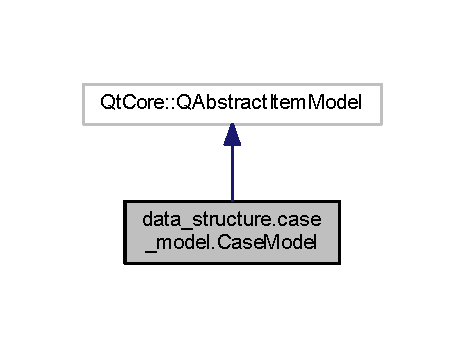
\includegraphics[width=223pt]{classdata__structure_1_1case__model_1_1_case_model__inherit__graph}
\end{center}
\end{figure}
\subsection*{Public Member Functions}
\begin{DoxyCompactItemize}
\item 
def \hyperlink{classdata__structure_1_1case__model_1_1_case_model_a7961b552537902b9236c2ded9cbfbc63}{\+\_\+\+\_\+init\+\_\+\+\_\+} (self, root, \hyperlink{classdata__structure_1_1case__model_1_1_case_model_afa98c784f58d15bdb49c9ba85854ae03}{parent}=None)
\item 
def \hyperlink{classdata__structure_1_1case__model_1_1_case_model_a44b390eef57be2a4883c1e6599b5a8ca}{row\+Count} (self, \hyperlink{classdata__structure_1_1case__model_1_1_case_model_afa98c784f58d15bdb49c9ba85854ae03}{parent})
\item 
def \hyperlink{classdata__structure_1_1case__model_1_1_case_model_a132b1b7d95f07cae505b40b7fdeb4545}{column\+Count} (self, \hyperlink{classdata__structure_1_1case__model_1_1_case_model_afa98c784f58d15bdb49c9ba85854ae03}{parent})
\item 
def \hyperlink{classdata__structure_1_1case__model_1_1_case_model_a2f7291849d0efb3d7cff499d1cde0bf6}{data} (self, \hyperlink{classdata__structure_1_1case__model_1_1_case_model_a3c52ee6daea1dc2ce7bb23833c761ed2}{index}, role)
\begin{DoxyCompactList}\small\item\em Returns the data stored under the given role for the item referred to by the index. \end{DoxyCompactList}\item 
def \hyperlink{classdata__structure_1_1case__model_1_1_case_model_a9d7790fb94587e15b2c1b77a01e7845c}{set\+Data} (self, \hyperlink{classdata__structure_1_1case__model_1_1_case_model_a3c52ee6daea1dc2ce7bb23833c761ed2}{index}, value, role=Qt\+Core.\+Qt.\+Edit\+Role)
\item 
def \hyperlink{classdata__structure_1_1case__model_1_1_case_model_a6a1656f6697b334ba6112c194cf04611}{header\+Data} (self, section, orientation, role)
\item 
def \hyperlink{classdata__structure_1_1case__model_1_1_case_model_ad60d9395ff571be3fcf12411886f8bcf}{flags} (self, \hyperlink{classdata__structure_1_1case__model_1_1_case_model_a3c52ee6daea1dc2ce7bb23833c761ed2}{index})
\item 
def \hyperlink{classdata__structure_1_1case__model_1_1_case_model_afa98c784f58d15bdb49c9ba85854ae03}{parent} (self, \hyperlink{classdata__structure_1_1case__model_1_1_case_model_a3c52ee6daea1dc2ce7bb23833c761ed2}{index})
\item 
def \hyperlink{classdata__structure_1_1case__model_1_1_case_model_a3c52ee6daea1dc2ce7bb23833c761ed2}{index} (self, row, column, \hyperlink{classdata__structure_1_1case__model_1_1_case_model_afa98c784f58d15bdb49c9ba85854ae03}{parent})
\item 
def \hyperlink{classdata__structure_1_1case__model_1_1_case_model_ad19222ac3eb114c51dce157ae50b2e19}{get\+Node} (self, \hyperlink{classdata__structure_1_1case__model_1_1_case_model_a3c52ee6daea1dc2ce7bb23833c761ed2}{index})
\item 
def \hyperlink{classdata__structure_1_1case__model_1_1_case_model_aa80631169f93be117b17729ae8fa7bf6}{remove\+Rows} (self, position, rows, \hyperlink{classdata__structure_1_1case__model_1_1_case_model_afa98c784f58d15bdb49c9ba85854ae03}{parent}=Qt\+Core.\+Q\+Model\+Index())
\end{DoxyCompactItemize}


\subsection{Detailed Description}
This is a creation of a model for the tree view list. 

It inherits the basic Q\+Abstract\+Item\+Model class\+The Q\+Abstract\+Item\+Model class defines the standard interface that item models must use to be able to inter-\/operate with other components in the model/view architecture. It is not supposed to be instantiated directly. Instead, you should subclass it to create new models. This model will be the one used by a a \hyperlink{classdata__structure_1_1case__node_1_1_case_node}{data\+\_\+structure.\+case\+\_\+node.\+Case\+Node} object.

When subclassing Q\+Abstract\+Item\+Model, at the very least you must implement \hyperlink{classdata__structure_1_1case__model_1_1_case_model_a3c52ee6daea1dc2ce7bb23833c761ed2}{index()}, \hyperlink{classdata__structure_1_1case__model_1_1_case_model_afa98c784f58d15bdb49c9ba85854ae03}{parent()}, \hyperlink{classdata__structure_1_1case__model_1_1_case_model_a44b390eef57be2a4883c1e6599b5a8ca}{row\+Count()}, \hyperlink{classdata__structure_1_1case__model_1_1_case_model_a132b1b7d95f07cae505b40b7fdeb4545}{column\+Count()}, and \hyperlink{classdata__structure_1_1case__model_1_1_case_model_a2f7291849d0efb3d7cff499d1cde0bf6}{data()}. These functions are used in all read-\/only models, and form the basis of editable models. More info\+: \href{http://doc.qt.io/qt-5/qabstractitemmodel.html#details}{\tt http\+://doc.\+qt.\+io/qt-\/5/qabstractitemmodel.\+html\#details} 

\subsection{Constructor \& Destructor Documentation}
\hypertarget{classdata__structure_1_1case__model_1_1_case_model_a7961b552537902b9236c2ded9cbfbc63}{}\label{classdata__structure_1_1case__model_1_1_case_model_a7961b552537902b9236c2ded9cbfbc63} 
\index{data\+\_\+structure\+::case\+\_\+model\+::\+Case\+Model@{data\+\_\+structure\+::case\+\_\+model\+::\+Case\+Model}!\+\_\+\+\_\+init\+\_\+\+\_\+@{\+\_\+\+\_\+init\+\_\+\+\_\+}}
\index{\+\_\+\+\_\+init\+\_\+\+\_\+@{\+\_\+\+\_\+init\+\_\+\+\_\+}!data\+\_\+structure\+::case\+\_\+model\+::\+Case\+Model@{data\+\_\+structure\+::case\+\_\+model\+::\+Case\+Model}}
\subsubsection{\texorpdfstring{\+\_\+\+\_\+init\+\_\+\+\_\+()}{\_\_init\_\_()}}
{\footnotesize\ttfamily def data\+\_\+structure.\+case\+\_\+model.\+Case\+Model.\+\_\+\+\_\+init\+\_\+\+\_\+ (\begin{DoxyParamCaption}\item[{}]{self,  }\item[{}]{root,  }\item[{}]{parent = {\ttfamily None} }\end{DoxyParamCaption})}



\subsection{Member Function Documentation}
\hypertarget{classdata__structure_1_1case__model_1_1_case_model_a132b1b7d95f07cae505b40b7fdeb4545}{}\label{classdata__structure_1_1case__model_1_1_case_model_a132b1b7d95f07cae505b40b7fdeb4545} 
\index{data\+\_\+structure\+::case\+\_\+model\+::\+Case\+Model@{data\+\_\+structure\+::case\+\_\+model\+::\+Case\+Model}!column\+Count@{column\+Count}}
\index{column\+Count@{column\+Count}!data\+\_\+structure\+::case\+\_\+model\+::\+Case\+Model@{data\+\_\+structure\+::case\+\_\+model\+::\+Case\+Model}}
\subsubsection{\texorpdfstring{column\+Count()}{columnCount()}}
{\footnotesize\ttfamily def data\+\_\+structure.\+case\+\_\+model.\+Case\+Model.\+column\+Count (\begin{DoxyParamCaption}\item[{}]{self,  }\item[{}]{parent }\end{DoxyParamCaption})}

\hypertarget{classdata__structure_1_1case__model_1_1_case_model_a2f7291849d0efb3d7cff499d1cde0bf6}{}\label{classdata__structure_1_1case__model_1_1_case_model_a2f7291849d0efb3d7cff499d1cde0bf6} 
\index{data\+\_\+structure\+::case\+\_\+model\+::\+Case\+Model@{data\+\_\+structure\+::case\+\_\+model\+::\+Case\+Model}!data@{data}}
\index{data@{data}!data\+\_\+structure\+::case\+\_\+model\+::\+Case\+Model@{data\+\_\+structure\+::case\+\_\+model\+::\+Case\+Model}}
\subsubsection{\texorpdfstring{data()}{data()}}
{\footnotesize\ttfamily def data\+\_\+structure.\+case\+\_\+model.\+Case\+Model.\+data (\begin{DoxyParamCaption}\item[{}]{self,  }\item[{}]{index,  }\item[{}]{role }\end{DoxyParamCaption})}



Returns the data stored under the given role for the item referred to by the index. 

\hypertarget{classdata__structure_1_1case__model_1_1_case_model_ad60d9395ff571be3fcf12411886f8bcf}{}\label{classdata__structure_1_1case__model_1_1_case_model_ad60d9395ff571be3fcf12411886f8bcf} 
\index{data\+\_\+structure\+::case\+\_\+model\+::\+Case\+Model@{data\+\_\+structure\+::case\+\_\+model\+::\+Case\+Model}!flags@{flags}}
\index{flags@{flags}!data\+\_\+structure\+::case\+\_\+model\+::\+Case\+Model@{data\+\_\+structure\+::case\+\_\+model\+::\+Case\+Model}}
\subsubsection{\texorpdfstring{flags()}{flags()}}
{\footnotesize\ttfamily def data\+\_\+structure.\+case\+\_\+model.\+Case\+Model.\+flags (\begin{DoxyParamCaption}\item[{}]{self,  }\item[{}]{index }\end{DoxyParamCaption})}

\hypertarget{classdata__structure_1_1case__model_1_1_case_model_ad19222ac3eb114c51dce157ae50b2e19}{}\label{classdata__structure_1_1case__model_1_1_case_model_ad19222ac3eb114c51dce157ae50b2e19} 
\index{data\+\_\+structure\+::case\+\_\+model\+::\+Case\+Model@{data\+\_\+structure\+::case\+\_\+model\+::\+Case\+Model}!get\+Node@{get\+Node}}
\index{get\+Node@{get\+Node}!data\+\_\+structure\+::case\+\_\+model\+::\+Case\+Model@{data\+\_\+structure\+::case\+\_\+model\+::\+Case\+Model}}
\subsubsection{\texorpdfstring{get\+Node()}{getNode()}}
{\footnotesize\ttfamily def data\+\_\+structure.\+case\+\_\+model.\+Case\+Model.\+get\+Node (\begin{DoxyParamCaption}\item[{}]{self,  }\item[{}]{index }\end{DoxyParamCaption})}

\hypertarget{classdata__structure_1_1case__model_1_1_case_model_a6a1656f6697b334ba6112c194cf04611}{}\label{classdata__structure_1_1case__model_1_1_case_model_a6a1656f6697b334ba6112c194cf04611} 
\index{data\+\_\+structure\+::case\+\_\+model\+::\+Case\+Model@{data\+\_\+structure\+::case\+\_\+model\+::\+Case\+Model}!header\+Data@{header\+Data}}
\index{header\+Data@{header\+Data}!data\+\_\+structure\+::case\+\_\+model\+::\+Case\+Model@{data\+\_\+structure\+::case\+\_\+model\+::\+Case\+Model}}
\subsubsection{\texorpdfstring{header\+Data()}{headerData()}}
{\footnotesize\ttfamily def data\+\_\+structure.\+case\+\_\+model.\+Case\+Model.\+header\+Data (\begin{DoxyParamCaption}\item[{}]{self,  }\item[{}]{section,  }\item[{}]{orientation,  }\item[{}]{role }\end{DoxyParamCaption})}

\hypertarget{classdata__structure_1_1case__model_1_1_case_model_a3c52ee6daea1dc2ce7bb23833c761ed2}{}\label{classdata__structure_1_1case__model_1_1_case_model_a3c52ee6daea1dc2ce7bb23833c761ed2} 
\index{data\+\_\+structure\+::case\+\_\+model\+::\+Case\+Model@{data\+\_\+structure\+::case\+\_\+model\+::\+Case\+Model}!index@{index}}
\index{index@{index}!data\+\_\+structure\+::case\+\_\+model\+::\+Case\+Model@{data\+\_\+structure\+::case\+\_\+model\+::\+Case\+Model}}
\subsubsection{\texorpdfstring{index()}{index()}}
{\footnotesize\ttfamily def data\+\_\+structure.\+case\+\_\+model.\+Case\+Model.\+index (\begin{DoxyParamCaption}\item[{}]{self,  }\item[{}]{row,  }\item[{}]{column,  }\item[{}]{parent }\end{DoxyParamCaption})}

\hypertarget{classdata__structure_1_1case__model_1_1_case_model_afa98c784f58d15bdb49c9ba85854ae03}{}\label{classdata__structure_1_1case__model_1_1_case_model_afa98c784f58d15bdb49c9ba85854ae03} 
\index{data\+\_\+structure\+::case\+\_\+model\+::\+Case\+Model@{data\+\_\+structure\+::case\+\_\+model\+::\+Case\+Model}!parent@{parent}}
\index{parent@{parent}!data\+\_\+structure\+::case\+\_\+model\+::\+Case\+Model@{data\+\_\+structure\+::case\+\_\+model\+::\+Case\+Model}}
\subsubsection{\texorpdfstring{parent()}{parent()}}
{\footnotesize\ttfamily def data\+\_\+structure.\+case\+\_\+model.\+Case\+Model.\+parent (\begin{DoxyParamCaption}\item[{}]{self,  }\item[{}]{index }\end{DoxyParamCaption})}

\hypertarget{classdata__structure_1_1case__model_1_1_case_model_aa80631169f93be117b17729ae8fa7bf6}{}\label{classdata__structure_1_1case__model_1_1_case_model_aa80631169f93be117b17729ae8fa7bf6} 
\index{data\+\_\+structure\+::case\+\_\+model\+::\+Case\+Model@{data\+\_\+structure\+::case\+\_\+model\+::\+Case\+Model}!remove\+Rows@{remove\+Rows}}
\index{remove\+Rows@{remove\+Rows}!data\+\_\+structure\+::case\+\_\+model\+::\+Case\+Model@{data\+\_\+structure\+::case\+\_\+model\+::\+Case\+Model}}
\subsubsection{\texorpdfstring{remove\+Rows()}{removeRows()}}
{\footnotesize\ttfamily def data\+\_\+structure.\+case\+\_\+model.\+Case\+Model.\+remove\+Rows (\begin{DoxyParamCaption}\item[{}]{self,  }\item[{}]{position,  }\item[{}]{rows,  }\item[{}]{parent = {\ttfamily QtCore.QModelIndex()} }\end{DoxyParamCaption})}

\hypertarget{classdata__structure_1_1case__model_1_1_case_model_a44b390eef57be2a4883c1e6599b5a8ca}{}\label{classdata__structure_1_1case__model_1_1_case_model_a44b390eef57be2a4883c1e6599b5a8ca} 
\index{data\+\_\+structure\+::case\+\_\+model\+::\+Case\+Model@{data\+\_\+structure\+::case\+\_\+model\+::\+Case\+Model}!row\+Count@{row\+Count}}
\index{row\+Count@{row\+Count}!data\+\_\+structure\+::case\+\_\+model\+::\+Case\+Model@{data\+\_\+structure\+::case\+\_\+model\+::\+Case\+Model}}
\subsubsection{\texorpdfstring{row\+Count()}{rowCount()}}
{\footnotesize\ttfamily def data\+\_\+structure.\+case\+\_\+model.\+Case\+Model.\+row\+Count (\begin{DoxyParamCaption}\item[{}]{self,  }\item[{}]{parent }\end{DoxyParamCaption})}

\hypertarget{classdata__structure_1_1case__model_1_1_case_model_a9d7790fb94587e15b2c1b77a01e7845c}{}\label{classdata__structure_1_1case__model_1_1_case_model_a9d7790fb94587e15b2c1b77a01e7845c} 
\index{data\+\_\+structure\+::case\+\_\+model\+::\+Case\+Model@{data\+\_\+structure\+::case\+\_\+model\+::\+Case\+Model}!set\+Data@{set\+Data}}
\index{set\+Data@{set\+Data}!data\+\_\+structure\+::case\+\_\+model\+::\+Case\+Model@{data\+\_\+structure\+::case\+\_\+model\+::\+Case\+Model}}
\subsubsection{\texorpdfstring{set\+Data()}{setData()}}
{\footnotesize\ttfamily def data\+\_\+structure.\+case\+\_\+model.\+Case\+Model.\+set\+Data (\begin{DoxyParamCaption}\item[{}]{self,  }\item[{}]{index,  }\item[{}]{value,  }\item[{}]{role = {\ttfamily QtCore.Qt.EditRole} }\end{DoxyParamCaption})}



The documentation for this class was generated from the following file\+:\begin{DoxyCompactItemize}
\item 
\hyperlink{case__model_8py}{case\+\_\+model.\+py}\end{DoxyCompactItemize}

\hypertarget{classdata__structure_1_1case__node_1_1_case_node}{}\section{data\+\_\+structure.\+case\+\_\+node.\+Case\+Node Class Reference}
\label{classdata__structure_1_1case__node_1_1_case_node}\index{data\+\_\+structure.\+case\+\_\+node.\+Case\+Node@{data\+\_\+structure.\+case\+\_\+node.\+Case\+Node}}


Class to structure all data loaded in \hyperlink{class_core_1_1_blade_py_core_a1a62f9b5b8f5929bdb6f0a8c27049d9e}{Core.\+Blade\+Py\+Core.\+add\+Case()}.  




Inheritance diagram for data\+\_\+structure.\+case\+\_\+node.\+Case\+Node\+:\nopagebreak
\begin{figure}[H]
\begin{center}
\leavevmode
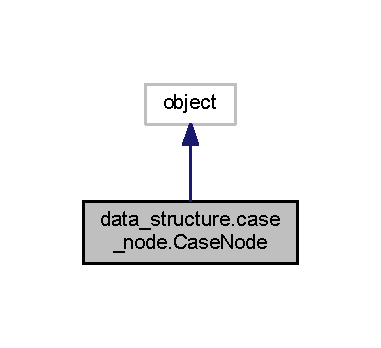
\includegraphics[width=183pt]{classdata__structure_1_1case__node_1_1_case_node__inherit__graph}
\end{center}
\end{figure}
\subsection*{Public Member Functions}
\begin{DoxyCompactItemize}
\item 
def \hyperlink{classdata__structure_1_1case__node_1_1_case_node_a268359dc0ff12ae9d60b0311f4d20a12}{\+\_\+\+\_\+init\+\_\+\+\_\+} (self, \hyperlink{classdata__structure_1_1case__node_1_1_case_node_a73e2e5313f50260c6c767fef3c4b3ced}{name}, shape=None, subshape\+\_\+names=None, plot\+\_\+lists=None, \hyperlink{classdata__structure_1_1case__node_1_1_case_node_a130f184f648103908a74a8a332f7513f}{parent}=None)
\begin{DoxyCompactList}\small\item\em The constructor of the class. \end{DoxyCompactList}\item 
def \hyperlink{classdata__structure_1_1case__node_1_1_case_node_ad3bd18eb2babab717bc4bd7a48ddbcb2}{shape\+H\+A\+IS} (self)
\begin{DoxyCompactList}\small\item\em Method for retrieving the handle of A\+I\+S\+\_\+\+Shape for the node. \end{DoxyCompactList}\item 
def \hyperlink{classdata__structure_1_1case__node_1_1_case_node_acc05e6147aac463ecd4b8073a050a54e}{shape\+Transformation} (self)
\begin{DoxyCompactList}\small\item\em Method for getting the transformation for the shape of this case. \end{DoxyCompactList}\item 
def \hyperlink{classdata__structure_1_1case__node_1_1_case_node_a4ee5ef91001b2c4db57c268338ef287e}{set\+Shape\+Transformation} (self, transformation, coord)
\begin{DoxyCompactList}\small\item\em Method for setting the transformation for the shape of this case. \end{DoxyCompactList}\item 
def \hyperlink{classdata__structure_1_1case__node_1_1_case_node_a7ee651fb0c3759df3d639ca19f70710d}{shape\+Transparency} (self)
\begin{DoxyCompactList}\small\item\em Method for getting the transparency for the shape of this case. \end{DoxyCompactList}\item 
def \hyperlink{classdata__structure_1_1case__node_1_1_case_node_ac24fbc54a83a04a8ea3d20f058b3a196}{set\+Shape\+Transparency} (self, transparency)
\begin{DoxyCompactList}\small\item\em Method for setting the transparency for the shape of this case. \end{DoxyCompactList}\item 
def \hyperlink{classdata__structure_1_1case__node_1_1_case_node_aedc74c039a8da3960544f0694e2379b0}{shape\+Color} (self)
\begin{DoxyCompactList}\small\item\em Method for getting the color for the shape of this case. \end{DoxyCompactList}\item 
def \hyperlink{classdata__structure_1_1case__node_1_1_case_node_a9eb860e45595b4a1c4d018c259d9d930}{set\+Shape\+Color} (self, color)
\begin{DoxyCompactList}\small\item\em Method for setting the color for the shape of this case. \end{DoxyCompactList}\item 
def \hyperlink{classdata__structure_1_1case__node_1_1_case_node_a333ce56e7787cb1d23974a75182facca}{shape\+Quality} (self)
\begin{DoxyCompactList}\small\item\em Method for getting the quality for the shape of this case. \end{DoxyCompactList}\item 
def \hyperlink{classdata__structure_1_1case__node_1_1_case_node_a7bc800f55127489e601b7ddbaa6ad2cb}{set\+Shape\+Quality} (self, quality)
\begin{DoxyCompactList}\small\item\em Method for setting the quality for the shape of this case. \end{DoxyCompactList}\item 
def \hyperlink{classdata__structure_1_1case__node_1_1_case_node_a5fda7f2cc9d0dd56ad8e088447decd15}{tecplot\+Lists} (self)
\begin{DoxyCompactList}\small\item\em Method for getting the tecplot graphics of this case. \end{DoxyCompactList}\item 
def \hyperlink{classdata__structure_1_1case__node_1_1_case_node_ae868c48f3c348062424b040c2e7f4646}{tecplot\+Saved\+Style\+List} (self)
\begin{DoxyCompactList}\small\item\em Method for getting the saved tecplot graphics line-\/styles of this case. \end{DoxyCompactList}\item 
def \hyperlink{classdata__structure_1_1case__node_1_1_case_node_aca41f53412a5bfdc6e3ced0ddaf3d2b3}{set\+Tecplot\+Saved\+Style\+List} (self, tecplot\+\_\+list)
\begin{DoxyCompactList}\small\item\em Method for setting the saved tecplot graphics line-\/styles of this case. \end{DoxyCompactList}\item 
def \hyperlink{classdata__structure_1_1case__node_1_1_case_node_aeb90281663e7094357befb23383a0d12}{tecplot\+Visibility} (self)
\begin{DoxyCompactList}\small\item\em Method for getting the current state of visibility the tecplot graphics for this case. \end{DoxyCompactList}\item 
def \hyperlink{classdata__structure_1_1case__node_1_1_case_node_a7bf258efc68a0aa850fd68d937b54d44}{set\+Tecplot\+Visibility} (self, visibility)
\begin{DoxyCompactList}\small\item\em Method for setting a state for the tecplot graphics for this case. \end{DoxyCompactList}\item 
def \hyperlink{classdata__structure_1_1case__node_1_1_case_node_adf31e8bf3222b4c310e652a08fa4cbb5}{tecplot\+Is\+Visible} (self)
\begin{DoxyCompactList}\small\item\em Method for verifying if tecplot is visible. \end{DoxyCompactList}\item 
def \hyperlink{classdata__structure_1_1case__node_1_1_case_node_aed14e2af89b145c93189f2e13b3520f9}{tecplot\+Mode} (self)
\begin{DoxyCompactList}\small\item\em Method for getting the current state of mode the tecplot graphics for this case. \end{DoxyCompactList}\item 
def \hyperlink{classdata__structure_1_1case__node_1_1_case_node_a18f8a870b09f2ec7c25bde6da6ad4d77}{set\+Tecplot\+Mode} (self, mode)
\begin{DoxyCompactList}\small\item\em Method for setting the current state of mode the tecplot graphics for this case. \end{DoxyCompactList}\item 
def \hyperlink{classdata__structure_1_1case__node_1_1_case_node_ac8139ea04504dbaedeeb295d2db40cd7}{tecplot\+Is\+Neutral} (self)
\begin{DoxyCompactList}\small\item\em Method for verifying if tecplot is neutral. \end{DoxyCompactList}\item 
def \hyperlink{classdata__structure_1_1case__node_1_1_case_node_a5be02db2416888d37bf33c148a97bc0c}{add\+Child} (self, \hyperlink{classdata__structure_1_1case__node_1_1_case_node_ac5303eb8bbab69954feaa7205ba778aa}{child})
\begin{DoxyCompactList}\small\item\em Methods required by model tree view of Py\+Qt. \end{DoxyCompactList}\item 
def \hyperlink{classdata__structure_1_1case__node_1_1_case_node_a9f706863d3146d479a3be6d7737a6102}{insert\+Child} (self, position, \hyperlink{classdata__structure_1_1case__node_1_1_case_node_ac5303eb8bbab69954feaa7205ba778aa}{child})
\begin{DoxyCompactList}\small\item\em Methods required by model tree view of Py\+Qt. \end{DoxyCompactList}\item 
def \hyperlink{classdata__structure_1_1case__node_1_1_case_node_ac40fac97e12433646432658373d17bb5}{remove\+Child} (self, position)
\begin{DoxyCompactList}\small\item\em Methods required by model tree view of Py\+Qt. \end{DoxyCompactList}\item 
def \hyperlink{classdata__structure_1_1case__node_1_1_case_node_a73e2e5313f50260c6c767fef3c4b3ced}{name} (self)
\begin{DoxyCompactList}\small\item\em Methods required by model tree view of Py\+Qt. \end{DoxyCompactList}\item 
def \hyperlink{classdata__structure_1_1case__node_1_1_case_node_ae3f38c3ce20582e74e659a1657282c0e}{set\+Name} (self, \hyperlink{classdata__structure_1_1case__node_1_1_case_node_a73e2e5313f50260c6c767fef3c4b3ced}{name})
\begin{DoxyCompactList}\small\item\em Methods required by model tree view of Py\+Qt. \end{DoxyCompactList}\item 
def \hyperlink{classdata__structure_1_1case__node_1_1_case_node_ac5303eb8bbab69954feaa7205ba778aa}{child} (self, \hyperlink{classdata__structure_1_1case__node_1_1_case_node_a5ffe67a35812f868b49b833deeae9e60}{row})
\begin{DoxyCompactList}\small\item\em Methods required by model tree view of Py\+Qt. \end{DoxyCompactList}\item 
def \hyperlink{classdata__structure_1_1case__node_1_1_case_node_a1151098cb931c0dac5e36b5a430ee831}{child\+Count} (self)
\begin{DoxyCompactList}\small\item\em Methods required by model tree view of Py\+Qt. \end{DoxyCompactList}\item 
def \hyperlink{classdata__structure_1_1case__node_1_1_case_node_a130f184f648103908a74a8a332f7513f}{parent} (self)
\begin{DoxyCompactList}\small\item\em Methods required by model tree view of Py\+Qt. \end{DoxyCompactList}\item 
def \hyperlink{classdata__structure_1_1case__node_1_1_case_node_a5ffe67a35812f868b49b833deeae9e60}{row} (self)
\begin{DoxyCompactList}\small\item\em Methods required by model tree view of Py\+Qt. \end{DoxyCompactList}\end{DoxyCompactItemize}
\subsection*{Public Attributes}
\begin{DoxyCompactItemize}
\item 
\hyperlink{classdata__structure_1_1case__node_1_1_case_node_ac2f5b0ae9715edeac8f9b1ccc0fd64e3}{subshape}
\end{DoxyCompactItemize}


\subsection{Detailed Description}
Class to structure all data loaded in \hyperlink{class_core_1_1_blade_py_core_a1a62f9b5b8f5929bdb6f0a8c27049d9e}{Core.\+Blade\+Py\+Core.\+add\+Case()}. 

This is the structure to be read by the model set to tree list view. The case node contains information of name of the case, handle of the ais\+\_\+shape, the name of the sub-\/shapes in the loaded igs and the graphics generate by Tecplot\+Reader Widget. The model used to represent a \hyperlink{classdata__structure_1_1case__node_1_1_case_node}{Case\+Node} is an \hyperlink{classdata__structure_1_1case__model_1_1_case_model}{case\+\_\+model.\+Case\+Model} object. 

\subsection{Constructor \& Destructor Documentation}
\hypertarget{classdata__structure_1_1case__node_1_1_case_node_a268359dc0ff12ae9d60b0311f4d20a12}{}\label{classdata__structure_1_1case__node_1_1_case_node_a268359dc0ff12ae9d60b0311f4d20a12} 
\index{data\+\_\+structure\+::case\+\_\+node\+::\+Case\+Node@{data\+\_\+structure\+::case\+\_\+node\+::\+Case\+Node}!\+\_\+\+\_\+init\+\_\+\+\_\+@{\+\_\+\+\_\+init\+\_\+\+\_\+}}
\index{\+\_\+\+\_\+init\+\_\+\+\_\+@{\+\_\+\+\_\+init\+\_\+\+\_\+}!data\+\_\+structure\+::case\+\_\+node\+::\+Case\+Node@{data\+\_\+structure\+::case\+\_\+node\+::\+Case\+Node}}
\subsubsection{\texorpdfstring{\+\_\+\+\_\+init\+\_\+\+\_\+()}{\_\_init\_\_()}}
{\footnotesize\ttfamily def data\+\_\+structure.\+case\+\_\+node.\+Case\+Node.\+\_\+\+\_\+init\+\_\+\+\_\+ (\begin{DoxyParamCaption}\item[{}]{self,  }\item[{}]{name,  }\item[{}]{shape = {\ttfamily None},  }\item[{}]{subshape\+\_\+names = {\ttfamily None},  }\item[{}]{plot\+\_\+lists = {\ttfamily None},  }\item[{}]{parent = {\ttfamily None} }\end{DoxyParamCaption})}



The constructor of the class. 

A \hyperlink{classdata__structure_1_1case__node_1_1_case_node}{Case\+Node} object is created in \hyperlink{class_core_1_1_blade_py_core_a1a62f9b5b8f5929bdb6f0a8c27049d9e}{Core.\+Blade\+Py\+Core.\+add\+Case()}


\begin{DoxyParams}{Parameters}
{\em name} & \mbox{[}str\mbox{]} Name of the case \\
\hline
{\em shape} & \mbox{[}Handle\+\_\+\+A\+I\+S\+\_\+\+Interactive\+Object\mbox{]} Handles of A\+I\+S\+\_\+\+Shape for shape controlling \\
\hline
{\em plot\+\_\+lists} & \mbox{[}list\mbox{]} List of lists of graphics generated by Tecplot\+Reader \\
\hline
{\em subshape\+\_\+names} & \mbox{[}list\mbox{]} List of strings of sub-\/shapes names. \\
\hline
{\em parent} & \mbox{[}\hyperlink{classdata__structure_1_1case__node_1_1_case_node}{Case\+Node}\mbox{]} Is a \hyperlink{classdata__structure_1_1case__node_1_1_case_node}{Case\+Node} object itself. It is the parent of the node. \\
\hline
\end{DoxyParams}


\subsection{Member Function Documentation}
\hypertarget{classdata__structure_1_1case__node_1_1_case_node_a5be02db2416888d37bf33c148a97bc0c}{}\label{classdata__structure_1_1case__node_1_1_case_node_a5be02db2416888d37bf33c148a97bc0c} 
\index{data\+\_\+structure\+::case\+\_\+node\+::\+Case\+Node@{data\+\_\+structure\+::case\+\_\+node\+::\+Case\+Node}!add\+Child@{add\+Child}}
\index{add\+Child@{add\+Child}!data\+\_\+structure\+::case\+\_\+node\+::\+Case\+Node@{data\+\_\+structure\+::case\+\_\+node\+::\+Case\+Node}}
\subsubsection{\texorpdfstring{add\+Child()}{addChild()}}
{\footnotesize\ttfamily def data\+\_\+structure.\+case\+\_\+node.\+Case\+Node.\+add\+Child (\begin{DoxyParamCaption}\item[{}]{self,  }\item[{}]{child }\end{DoxyParamCaption})}



Methods required by model tree view of Py\+Qt. 

Not necessary to observe this method. \hypertarget{classdata__structure_1_1case__node_1_1_case_node_ac5303eb8bbab69954feaa7205ba778aa}{}\label{classdata__structure_1_1case__node_1_1_case_node_ac5303eb8bbab69954feaa7205ba778aa} 
\index{data\+\_\+structure\+::case\+\_\+node\+::\+Case\+Node@{data\+\_\+structure\+::case\+\_\+node\+::\+Case\+Node}!child@{child}}
\index{child@{child}!data\+\_\+structure\+::case\+\_\+node\+::\+Case\+Node@{data\+\_\+structure\+::case\+\_\+node\+::\+Case\+Node}}
\subsubsection{\texorpdfstring{child()}{child()}}
{\footnotesize\ttfamily def data\+\_\+structure.\+case\+\_\+node.\+Case\+Node.\+child (\begin{DoxyParamCaption}\item[{}]{self,  }\item[{}]{row }\end{DoxyParamCaption})}



Methods required by model tree view of Py\+Qt. 

Not necessary to observe this method. \hypertarget{classdata__structure_1_1case__node_1_1_case_node_a1151098cb931c0dac5e36b5a430ee831}{}\label{classdata__structure_1_1case__node_1_1_case_node_a1151098cb931c0dac5e36b5a430ee831} 
\index{data\+\_\+structure\+::case\+\_\+node\+::\+Case\+Node@{data\+\_\+structure\+::case\+\_\+node\+::\+Case\+Node}!child\+Count@{child\+Count}}
\index{child\+Count@{child\+Count}!data\+\_\+structure\+::case\+\_\+node\+::\+Case\+Node@{data\+\_\+structure\+::case\+\_\+node\+::\+Case\+Node}}
\subsubsection{\texorpdfstring{child\+Count()}{childCount()}}
{\footnotesize\ttfamily def data\+\_\+structure.\+case\+\_\+node.\+Case\+Node.\+child\+Count (\begin{DoxyParamCaption}\item[{}]{self }\end{DoxyParamCaption})}



Methods required by model tree view of Py\+Qt. 

Not necessary to observe this method. \hypertarget{classdata__structure_1_1case__node_1_1_case_node_a9f706863d3146d479a3be6d7737a6102}{}\label{classdata__structure_1_1case__node_1_1_case_node_a9f706863d3146d479a3be6d7737a6102} 
\index{data\+\_\+structure\+::case\+\_\+node\+::\+Case\+Node@{data\+\_\+structure\+::case\+\_\+node\+::\+Case\+Node}!insert\+Child@{insert\+Child}}
\index{insert\+Child@{insert\+Child}!data\+\_\+structure\+::case\+\_\+node\+::\+Case\+Node@{data\+\_\+structure\+::case\+\_\+node\+::\+Case\+Node}}
\subsubsection{\texorpdfstring{insert\+Child()}{insertChild()}}
{\footnotesize\ttfamily def data\+\_\+structure.\+case\+\_\+node.\+Case\+Node.\+insert\+Child (\begin{DoxyParamCaption}\item[{}]{self,  }\item[{}]{position,  }\item[{}]{child }\end{DoxyParamCaption})}



Methods required by model tree view of Py\+Qt. 

Not necessary to observe this method. \hypertarget{classdata__structure_1_1case__node_1_1_case_node_a73e2e5313f50260c6c767fef3c4b3ced}{}\label{classdata__structure_1_1case__node_1_1_case_node_a73e2e5313f50260c6c767fef3c4b3ced} 
\index{data\+\_\+structure\+::case\+\_\+node\+::\+Case\+Node@{data\+\_\+structure\+::case\+\_\+node\+::\+Case\+Node}!name@{name}}
\index{name@{name}!data\+\_\+structure\+::case\+\_\+node\+::\+Case\+Node@{data\+\_\+structure\+::case\+\_\+node\+::\+Case\+Node}}
\subsubsection{\texorpdfstring{name()}{name()}}
{\footnotesize\ttfamily def data\+\_\+structure.\+case\+\_\+node.\+Case\+Node.\+name (\begin{DoxyParamCaption}\item[{}]{self }\end{DoxyParamCaption})}



Methods required by model tree view of Py\+Qt. 

Not necessary to observe this method. \hypertarget{classdata__structure_1_1case__node_1_1_case_node_a130f184f648103908a74a8a332f7513f}{}\label{classdata__structure_1_1case__node_1_1_case_node_a130f184f648103908a74a8a332f7513f} 
\index{data\+\_\+structure\+::case\+\_\+node\+::\+Case\+Node@{data\+\_\+structure\+::case\+\_\+node\+::\+Case\+Node}!parent@{parent}}
\index{parent@{parent}!data\+\_\+structure\+::case\+\_\+node\+::\+Case\+Node@{data\+\_\+structure\+::case\+\_\+node\+::\+Case\+Node}}
\subsubsection{\texorpdfstring{parent()}{parent()}}
{\footnotesize\ttfamily def data\+\_\+structure.\+case\+\_\+node.\+Case\+Node.\+parent (\begin{DoxyParamCaption}\item[{}]{self }\end{DoxyParamCaption})}



Methods required by model tree view of Py\+Qt. 

Not necessary to observe this method. \hypertarget{classdata__structure_1_1case__node_1_1_case_node_ac40fac97e12433646432658373d17bb5}{}\label{classdata__structure_1_1case__node_1_1_case_node_ac40fac97e12433646432658373d17bb5} 
\index{data\+\_\+structure\+::case\+\_\+node\+::\+Case\+Node@{data\+\_\+structure\+::case\+\_\+node\+::\+Case\+Node}!remove\+Child@{remove\+Child}}
\index{remove\+Child@{remove\+Child}!data\+\_\+structure\+::case\+\_\+node\+::\+Case\+Node@{data\+\_\+structure\+::case\+\_\+node\+::\+Case\+Node}}
\subsubsection{\texorpdfstring{remove\+Child()}{removeChild()}}
{\footnotesize\ttfamily def data\+\_\+structure.\+case\+\_\+node.\+Case\+Node.\+remove\+Child (\begin{DoxyParamCaption}\item[{}]{self,  }\item[{}]{position }\end{DoxyParamCaption})}



Methods required by model tree view of Py\+Qt. 

Not necessary to observe this method. \hypertarget{classdata__structure_1_1case__node_1_1_case_node_a5ffe67a35812f868b49b833deeae9e60}{}\label{classdata__structure_1_1case__node_1_1_case_node_a5ffe67a35812f868b49b833deeae9e60} 
\index{data\+\_\+structure\+::case\+\_\+node\+::\+Case\+Node@{data\+\_\+structure\+::case\+\_\+node\+::\+Case\+Node}!row@{row}}
\index{row@{row}!data\+\_\+structure\+::case\+\_\+node\+::\+Case\+Node@{data\+\_\+structure\+::case\+\_\+node\+::\+Case\+Node}}
\subsubsection{\texorpdfstring{row()}{row()}}
{\footnotesize\ttfamily def data\+\_\+structure.\+case\+\_\+node.\+Case\+Node.\+row (\begin{DoxyParamCaption}\item[{}]{self }\end{DoxyParamCaption})}



Methods required by model tree view of Py\+Qt. 

Not necessary to observe this method. \hypertarget{classdata__structure_1_1case__node_1_1_case_node_ae3f38c3ce20582e74e659a1657282c0e}{}\label{classdata__structure_1_1case__node_1_1_case_node_ae3f38c3ce20582e74e659a1657282c0e} 
\index{data\+\_\+structure\+::case\+\_\+node\+::\+Case\+Node@{data\+\_\+structure\+::case\+\_\+node\+::\+Case\+Node}!set\+Name@{set\+Name}}
\index{set\+Name@{set\+Name}!data\+\_\+structure\+::case\+\_\+node\+::\+Case\+Node@{data\+\_\+structure\+::case\+\_\+node\+::\+Case\+Node}}
\subsubsection{\texorpdfstring{set\+Name()}{setName()}}
{\footnotesize\ttfamily def data\+\_\+structure.\+case\+\_\+node.\+Case\+Node.\+set\+Name (\begin{DoxyParamCaption}\item[{}]{self,  }\item[{}]{name }\end{DoxyParamCaption})}



Methods required by model tree view of Py\+Qt. 

Not necessary to observe this method. \hypertarget{classdata__structure_1_1case__node_1_1_case_node_a9eb860e45595b4a1c4d018c259d9d930}{}\label{classdata__structure_1_1case__node_1_1_case_node_a9eb860e45595b4a1c4d018c259d9d930} 
\index{data\+\_\+structure\+::case\+\_\+node\+::\+Case\+Node@{data\+\_\+structure\+::case\+\_\+node\+::\+Case\+Node}!set\+Shape\+Color@{set\+Shape\+Color}}
\index{set\+Shape\+Color@{set\+Shape\+Color}!data\+\_\+structure\+::case\+\_\+node\+::\+Case\+Node@{data\+\_\+structure\+::case\+\_\+node\+::\+Case\+Node}}
\subsubsection{\texorpdfstring{set\+Shape\+Color()}{setShapeColor()}}
{\footnotesize\ttfamily def data\+\_\+structure.\+case\+\_\+node.\+Case\+Node.\+set\+Shape\+Color (\begin{DoxyParamCaption}\item[{}]{self,  }\item[{}]{color }\end{DoxyParamCaption})}



Method for setting the color for the shape of this case. 


\begin{DoxyParams}{Parameters}
{\em color} & \mbox{[}int\mbox{]} The index of the color list of occ\+\_\+modules.\+shapeproperties.\+shape\+\_\+colorlist \\
\hline
\end{DoxyParams}
\begin{DoxyReturn}{Returns}
None 
\end{DoxyReturn}
\hypertarget{classdata__structure_1_1case__node_1_1_case_node_a7bc800f55127489e601b7ddbaa6ad2cb}{}\label{classdata__structure_1_1case__node_1_1_case_node_a7bc800f55127489e601b7ddbaa6ad2cb} 
\index{data\+\_\+structure\+::case\+\_\+node\+::\+Case\+Node@{data\+\_\+structure\+::case\+\_\+node\+::\+Case\+Node}!set\+Shape\+Quality@{set\+Shape\+Quality}}
\index{set\+Shape\+Quality@{set\+Shape\+Quality}!data\+\_\+structure\+::case\+\_\+node\+::\+Case\+Node@{data\+\_\+structure\+::case\+\_\+node\+::\+Case\+Node}}
\subsubsection{\texorpdfstring{set\+Shape\+Quality()}{setShapeQuality()}}
{\footnotesize\ttfamily def data\+\_\+structure.\+case\+\_\+node.\+Case\+Node.\+set\+Shape\+Quality (\begin{DoxyParamCaption}\item[{}]{self,  }\item[{}]{quality }\end{DoxyParamCaption})}



Method for setting the quality for the shape of this case. 


\begin{DoxyParams}{Parameters}
{\em quality} & \mbox{[}float\mbox{]} The quality of the shape of this case \\
\hline
\end{DoxyParams}
\begin{DoxyReturn}{Returns}
None 
\end{DoxyReturn}
\hypertarget{classdata__structure_1_1case__node_1_1_case_node_a4ee5ef91001b2c4db57c268338ef287e}{}\label{classdata__structure_1_1case__node_1_1_case_node_a4ee5ef91001b2c4db57c268338ef287e} 
\index{data\+\_\+structure\+::case\+\_\+node\+::\+Case\+Node@{data\+\_\+structure\+::case\+\_\+node\+::\+Case\+Node}!set\+Shape\+Transformation@{set\+Shape\+Transformation}}
\index{set\+Shape\+Transformation@{set\+Shape\+Transformation}!data\+\_\+structure\+::case\+\_\+node\+::\+Case\+Node@{data\+\_\+structure\+::case\+\_\+node\+::\+Case\+Node}}
\subsubsection{\texorpdfstring{set\+Shape\+Transformation()}{setShapeTransformation()}}
{\footnotesize\ttfamily def data\+\_\+structure.\+case\+\_\+node.\+Case\+Node.\+set\+Shape\+Transformation (\begin{DoxyParamCaption}\item[{}]{self,  }\item[{}]{transformation,  }\item[{}]{coord }\end{DoxyParamCaption})}



Method for setting the transformation for the shape of this case. 


\begin{DoxyParams}{Parameters}
{\em transformation} & \mbox{[}int\mbox{]} The value of transformation \\
\hline
{\em coord} & \mbox{[}int\mbox{]} Coordinate of transformation application. Indexes\+: \mbox{[}x\+:0, y\+:1, z\+:2, axis\+:3, theta\+:4\mbox{]}\\
\hline
\end{DoxyParams}
\begin{DoxyReturn}{Returns}
None 
\end{DoxyReturn}
\hypertarget{classdata__structure_1_1case__node_1_1_case_node_ac24fbc54a83a04a8ea3d20f058b3a196}{}\label{classdata__structure_1_1case__node_1_1_case_node_ac24fbc54a83a04a8ea3d20f058b3a196} 
\index{data\+\_\+structure\+::case\+\_\+node\+::\+Case\+Node@{data\+\_\+structure\+::case\+\_\+node\+::\+Case\+Node}!set\+Shape\+Transparency@{set\+Shape\+Transparency}}
\index{set\+Shape\+Transparency@{set\+Shape\+Transparency}!data\+\_\+structure\+::case\+\_\+node\+::\+Case\+Node@{data\+\_\+structure\+::case\+\_\+node\+::\+Case\+Node}}
\subsubsection{\texorpdfstring{set\+Shape\+Transparency()}{setShapeTransparency()}}
{\footnotesize\ttfamily def data\+\_\+structure.\+case\+\_\+node.\+Case\+Node.\+set\+Shape\+Transparency (\begin{DoxyParamCaption}\item[{}]{self,  }\item[{}]{transparency }\end{DoxyParamCaption})}



Method for setting the transparency for the shape of this case. 


\begin{DoxyParams}{Parameters}
{\em transparency} & \mbox{[}float\mbox{]} The value of transparency \\
\hline
\end{DoxyParams}
\begin{DoxyReturn}{Returns}
None 
\end{DoxyReturn}
\hypertarget{classdata__structure_1_1case__node_1_1_case_node_a18f8a870b09f2ec7c25bde6da6ad4d77}{}\label{classdata__structure_1_1case__node_1_1_case_node_a18f8a870b09f2ec7c25bde6da6ad4d77} 
\index{data\+\_\+structure\+::case\+\_\+node\+::\+Case\+Node@{data\+\_\+structure\+::case\+\_\+node\+::\+Case\+Node}!set\+Tecplot\+Mode@{set\+Tecplot\+Mode}}
\index{set\+Tecplot\+Mode@{set\+Tecplot\+Mode}!data\+\_\+structure\+::case\+\_\+node\+::\+Case\+Node@{data\+\_\+structure\+::case\+\_\+node\+::\+Case\+Node}}
\subsubsection{\texorpdfstring{set\+Tecplot\+Mode()}{setTecplotMode()}}
{\footnotesize\ttfamily def data\+\_\+structure.\+case\+\_\+node.\+Case\+Node.\+set\+Tecplot\+Mode (\begin{DoxyParamCaption}\item[{}]{self,  }\item[{}]{mode }\end{DoxyParamCaption})}



Method for setting the current state of mode the tecplot graphics for this case. 


\begin{DoxyParams}{Parameters}
{\em mode} & \mbox{[}str\mbox{]} The mode for this case. Can be \char`\"{}neutral\char`\"{} or \char`\"{}standard\char`\"{} \\
\hline
\end{DoxyParams}
\begin{DoxyReturn}{Returns}
None 
\end{DoxyReturn}
\hypertarget{classdata__structure_1_1case__node_1_1_case_node_aca41f53412a5bfdc6e3ced0ddaf3d2b3}{}\label{classdata__structure_1_1case__node_1_1_case_node_aca41f53412a5bfdc6e3ced0ddaf3d2b3} 
\index{data\+\_\+structure\+::case\+\_\+node\+::\+Case\+Node@{data\+\_\+structure\+::case\+\_\+node\+::\+Case\+Node}!set\+Tecplot\+Saved\+Style\+List@{set\+Tecplot\+Saved\+Style\+List}}
\index{set\+Tecplot\+Saved\+Style\+List@{set\+Tecplot\+Saved\+Style\+List}!data\+\_\+structure\+::case\+\_\+node\+::\+Case\+Node@{data\+\_\+structure\+::case\+\_\+node\+::\+Case\+Node}}
\subsubsection{\texorpdfstring{set\+Tecplot\+Saved\+Style\+List()}{setTecplotSavedStyleList()}}
{\footnotesize\ttfamily def data\+\_\+structure.\+case\+\_\+node.\+Case\+Node.\+set\+Tecplot\+Saved\+Style\+List (\begin{DoxyParamCaption}\item[{}]{self,  }\item[{}]{tecplot\+\_\+list }\end{DoxyParamCaption})}



Method for setting the saved tecplot graphics line-\/styles of this case. 

See datastructure.\+case\+\_\+node.\+tecplot\+Saved\+Style\+List()


\begin{DoxyParams}{Parameters}
{\em tecplot\+\_\+list} & \mbox{[}list\mbox{]} List of tecplot graphics line-\/styles to save \\
\hline
\end{DoxyParams}
\begin{DoxyReturn}{Returns}
None 
\end{DoxyReturn}
\hypertarget{classdata__structure_1_1case__node_1_1_case_node_a7bf258efc68a0aa850fd68d937b54d44}{}\label{classdata__structure_1_1case__node_1_1_case_node_a7bf258efc68a0aa850fd68d937b54d44} 
\index{data\+\_\+structure\+::case\+\_\+node\+::\+Case\+Node@{data\+\_\+structure\+::case\+\_\+node\+::\+Case\+Node}!set\+Tecplot\+Visibility@{set\+Tecplot\+Visibility}}
\index{set\+Tecplot\+Visibility@{set\+Tecplot\+Visibility}!data\+\_\+structure\+::case\+\_\+node\+::\+Case\+Node@{data\+\_\+structure\+::case\+\_\+node\+::\+Case\+Node}}
\subsubsection{\texorpdfstring{set\+Tecplot\+Visibility()}{setTecplotVisibility()}}
{\footnotesize\ttfamily def data\+\_\+structure.\+case\+\_\+node.\+Case\+Node.\+set\+Tecplot\+Visibility (\begin{DoxyParamCaption}\item[{}]{self,  }\item[{}]{visibility }\end{DoxyParamCaption})}



Method for setting a state for the tecplot graphics for this case. 


\begin{DoxyParams}{Parameters}
{\em visibility} & \mbox{[}str\mbox{]} The visibility for this case. Can be \char`\"{}visible\char`\"{} or \char`\"{}invisible\char`\"{} \\
\hline
\end{DoxyParams}
\begin{DoxyReturn}{Returns}
None 
\end{DoxyReturn}
\hypertarget{classdata__structure_1_1case__node_1_1_case_node_aedc74c039a8da3960544f0694e2379b0}{}\label{classdata__structure_1_1case__node_1_1_case_node_aedc74c039a8da3960544f0694e2379b0} 
\index{data\+\_\+structure\+::case\+\_\+node\+::\+Case\+Node@{data\+\_\+structure\+::case\+\_\+node\+::\+Case\+Node}!shape\+Color@{shape\+Color}}
\index{shape\+Color@{shape\+Color}!data\+\_\+structure\+::case\+\_\+node\+::\+Case\+Node@{data\+\_\+structure\+::case\+\_\+node\+::\+Case\+Node}}
\subsubsection{\texorpdfstring{shape\+Color()}{shapeColor()}}
{\footnotesize\ttfamily def data\+\_\+structure.\+case\+\_\+node.\+Case\+Node.\+shape\+Color (\begin{DoxyParamCaption}\item[{}]{self }\end{DoxyParamCaption})}



Method for getting the color for the shape of this case. 

\begin{DoxyReturn}{Returns}
\mbox{[}int\mbox{]} The index of the color list of occ\+\_\+modules.\+shapeproperties.\+shape\+\_\+colorlist 
\end{DoxyReturn}
\hypertarget{classdata__structure_1_1case__node_1_1_case_node_ad3bd18eb2babab717bc4bd7a48ddbcb2}{}\label{classdata__structure_1_1case__node_1_1_case_node_ad3bd18eb2babab717bc4bd7a48ddbcb2} 
\index{data\+\_\+structure\+::case\+\_\+node\+::\+Case\+Node@{data\+\_\+structure\+::case\+\_\+node\+::\+Case\+Node}!shape\+H\+A\+IS@{shape\+H\+A\+IS}}
\index{shape\+H\+A\+IS@{shape\+H\+A\+IS}!data\+\_\+structure\+::case\+\_\+node\+::\+Case\+Node@{data\+\_\+structure\+::case\+\_\+node\+::\+Case\+Node}}
\subsubsection{\texorpdfstring{shape\+H\+A\+I\+S()}{shapeHAIS()}}
{\footnotesize\ttfamily def data\+\_\+structure.\+case\+\_\+node.\+Case\+Node.\+shape\+H\+A\+IS (\begin{DoxyParamCaption}\item[{}]{self }\end{DoxyParamCaption})}



Method for retrieving the handle of A\+I\+S\+\_\+\+Shape for the node. 

\begin{DoxyReturn}{Returns}
\mbox{[}Handle\+\_\+\+A\+I\+S\+\_\+\+Interactive\+Object\mbox{]} The A\+I\+S\+\_\+shape Handle. 
\end{DoxyReturn}
\hypertarget{classdata__structure_1_1case__node_1_1_case_node_a333ce56e7787cb1d23974a75182facca}{}\label{classdata__structure_1_1case__node_1_1_case_node_a333ce56e7787cb1d23974a75182facca} 
\index{data\+\_\+structure\+::case\+\_\+node\+::\+Case\+Node@{data\+\_\+structure\+::case\+\_\+node\+::\+Case\+Node}!shape\+Quality@{shape\+Quality}}
\index{shape\+Quality@{shape\+Quality}!data\+\_\+structure\+::case\+\_\+node\+::\+Case\+Node@{data\+\_\+structure\+::case\+\_\+node\+::\+Case\+Node}}
\subsubsection{\texorpdfstring{shape\+Quality()}{shapeQuality()}}
{\footnotesize\ttfamily def data\+\_\+structure.\+case\+\_\+node.\+Case\+Node.\+shape\+Quality (\begin{DoxyParamCaption}\item[{}]{self }\end{DoxyParamCaption})}



Method for getting the quality for the shape of this case. 

\begin{DoxyReturn}{Returns}
\mbox{[}float\mbox{]} The quality of the shape of this case 
\end{DoxyReturn}
\hypertarget{classdata__structure_1_1case__node_1_1_case_node_acc05e6147aac463ecd4b8073a050a54e}{}\label{classdata__structure_1_1case__node_1_1_case_node_acc05e6147aac463ecd4b8073a050a54e} 
\index{data\+\_\+structure\+::case\+\_\+node\+::\+Case\+Node@{data\+\_\+structure\+::case\+\_\+node\+::\+Case\+Node}!shape\+Transformation@{shape\+Transformation}}
\index{shape\+Transformation@{shape\+Transformation}!data\+\_\+structure\+::case\+\_\+node\+::\+Case\+Node@{data\+\_\+structure\+::case\+\_\+node\+::\+Case\+Node}}
\subsubsection{\texorpdfstring{shape\+Transformation()}{shapeTransformation()}}
{\footnotesize\ttfamily def data\+\_\+structure.\+case\+\_\+node.\+Case\+Node.\+shape\+Transformation (\begin{DoxyParamCaption}\item[{}]{self }\end{DoxyParamCaption})}



Method for getting the transformation for the shape of this case. 

\begin{DoxyReturn}{Returns}
\mbox{[}list\mbox{]} The list of coordinates. 
\end{DoxyReturn}
\hypertarget{classdata__structure_1_1case__node_1_1_case_node_a7ee651fb0c3759df3d639ca19f70710d}{}\label{classdata__structure_1_1case__node_1_1_case_node_a7ee651fb0c3759df3d639ca19f70710d} 
\index{data\+\_\+structure\+::case\+\_\+node\+::\+Case\+Node@{data\+\_\+structure\+::case\+\_\+node\+::\+Case\+Node}!shape\+Transparency@{shape\+Transparency}}
\index{shape\+Transparency@{shape\+Transparency}!data\+\_\+structure\+::case\+\_\+node\+::\+Case\+Node@{data\+\_\+structure\+::case\+\_\+node\+::\+Case\+Node}}
\subsubsection{\texorpdfstring{shape\+Transparency()}{shapeTransparency()}}
{\footnotesize\ttfamily def data\+\_\+structure.\+case\+\_\+node.\+Case\+Node.\+shape\+Transparency (\begin{DoxyParamCaption}\item[{}]{self }\end{DoxyParamCaption})}



Method for getting the transparency for the shape of this case. 

\begin{DoxyReturn}{Returns}
\mbox{[}float\mbox{]} The transparency 
\end{DoxyReturn}
\hypertarget{classdata__structure_1_1case__node_1_1_case_node_ac8139ea04504dbaedeeb295d2db40cd7}{}\label{classdata__structure_1_1case__node_1_1_case_node_ac8139ea04504dbaedeeb295d2db40cd7} 
\index{data\+\_\+structure\+::case\+\_\+node\+::\+Case\+Node@{data\+\_\+structure\+::case\+\_\+node\+::\+Case\+Node}!tecplot\+Is\+Neutral@{tecplot\+Is\+Neutral}}
\index{tecplot\+Is\+Neutral@{tecplot\+Is\+Neutral}!data\+\_\+structure\+::case\+\_\+node\+::\+Case\+Node@{data\+\_\+structure\+::case\+\_\+node\+::\+Case\+Node}}
\subsubsection{\texorpdfstring{tecplot\+Is\+Neutral()}{tecplotIsNeutral()}}
{\footnotesize\ttfamily def data\+\_\+structure.\+case\+\_\+node.\+Case\+Node.\+tecplot\+Is\+Neutral (\begin{DoxyParamCaption}\item[{}]{self }\end{DoxyParamCaption})}



Method for verifying if tecplot is neutral. 

\begin{DoxyReturn}{Returns}
\mbox{[}bool\mbox{]} True if it is \char`\"{}neutral\char`\"{} False if it is \char`\"{}standard\char`\"{} 
\end{DoxyReturn}
\hypertarget{classdata__structure_1_1case__node_1_1_case_node_adf31e8bf3222b4c310e652a08fa4cbb5}{}\label{classdata__structure_1_1case__node_1_1_case_node_adf31e8bf3222b4c310e652a08fa4cbb5} 
\index{data\+\_\+structure\+::case\+\_\+node\+::\+Case\+Node@{data\+\_\+structure\+::case\+\_\+node\+::\+Case\+Node}!tecplot\+Is\+Visible@{tecplot\+Is\+Visible}}
\index{tecplot\+Is\+Visible@{tecplot\+Is\+Visible}!data\+\_\+structure\+::case\+\_\+node\+::\+Case\+Node@{data\+\_\+structure\+::case\+\_\+node\+::\+Case\+Node}}
\subsubsection{\texorpdfstring{tecplot\+Is\+Visible()}{tecplotIsVisible()}}
{\footnotesize\ttfamily def data\+\_\+structure.\+case\+\_\+node.\+Case\+Node.\+tecplot\+Is\+Visible (\begin{DoxyParamCaption}\item[{}]{self }\end{DoxyParamCaption})}



Method for verifying if tecplot is visible. 

\begin{DoxyReturn}{Returns}
\mbox{[}bool\mbox{]} True if it is \char`\"{}visible\char`\"{} False if it is \char`\"{}invisible\char`\"{} 
\end{DoxyReturn}
\hypertarget{classdata__structure_1_1case__node_1_1_case_node_a5fda7f2cc9d0dd56ad8e088447decd15}{}\label{classdata__structure_1_1case__node_1_1_case_node_a5fda7f2cc9d0dd56ad8e088447decd15} 
\index{data\+\_\+structure\+::case\+\_\+node\+::\+Case\+Node@{data\+\_\+structure\+::case\+\_\+node\+::\+Case\+Node}!tecplot\+Lists@{tecplot\+Lists}}
\index{tecplot\+Lists@{tecplot\+Lists}!data\+\_\+structure\+::case\+\_\+node\+::\+Case\+Node@{data\+\_\+structure\+::case\+\_\+node\+::\+Case\+Node}}
\subsubsection{\texorpdfstring{tecplot\+Lists()}{tecplotLists()}}
{\footnotesize\ttfamily def data\+\_\+structure.\+case\+\_\+node.\+Case\+Node.\+tecplot\+Lists (\begin{DoxyParamCaption}\item[{}]{self }\end{DoxyParamCaption})}



Method for getting the tecplot graphics of this case. 

\begin{DoxyReturn}{Returns}
\mbox{[}list\mbox{]} List of tecplots lines 
\end{DoxyReturn}
\hypertarget{classdata__structure_1_1case__node_1_1_case_node_aed14e2af89b145c93189f2e13b3520f9}{}\label{classdata__structure_1_1case__node_1_1_case_node_aed14e2af89b145c93189f2e13b3520f9} 
\index{data\+\_\+structure\+::case\+\_\+node\+::\+Case\+Node@{data\+\_\+structure\+::case\+\_\+node\+::\+Case\+Node}!tecplot\+Mode@{tecplot\+Mode}}
\index{tecplot\+Mode@{tecplot\+Mode}!data\+\_\+structure\+::case\+\_\+node\+::\+Case\+Node@{data\+\_\+structure\+::case\+\_\+node\+::\+Case\+Node}}
\subsubsection{\texorpdfstring{tecplot\+Mode()}{tecplotMode()}}
{\footnotesize\ttfamily def data\+\_\+structure.\+case\+\_\+node.\+Case\+Node.\+tecplot\+Mode (\begin{DoxyParamCaption}\item[{}]{self }\end{DoxyParamCaption})}



Method for getting the current state of mode the tecplot graphics for this case. 

The mode is whether all the lines in tecplot graphics are neutral -\/ black -\/ and dashed.

\begin{DoxyReturn}{Returns}
\mbox{[}str\mbox{]} The state of mode of the tecplot. Can be \char`\"{}neutral\char`\"{} or \char`\"{}standard\char`\"{} 
\end{DoxyReturn}
\hypertarget{classdata__structure_1_1case__node_1_1_case_node_ae868c48f3c348062424b040c2e7f4646}{}\label{classdata__structure_1_1case__node_1_1_case_node_ae868c48f3c348062424b040c2e7f4646} 
\index{data\+\_\+structure\+::case\+\_\+node\+::\+Case\+Node@{data\+\_\+structure\+::case\+\_\+node\+::\+Case\+Node}!tecplot\+Saved\+Style\+List@{tecplot\+Saved\+Style\+List}}
\index{tecplot\+Saved\+Style\+List@{tecplot\+Saved\+Style\+List}!data\+\_\+structure\+::case\+\_\+node\+::\+Case\+Node@{data\+\_\+structure\+::case\+\_\+node\+::\+Case\+Node}}
\subsubsection{\texorpdfstring{tecplot\+Saved\+Style\+List()}{tecplotSavedStyleList()}}
{\footnotesize\ttfamily def data\+\_\+structure.\+case\+\_\+node.\+Case\+Node.\+tecplot\+Saved\+Style\+List (\begin{DoxyParamCaption}\item[{}]{self }\end{DoxyParamCaption})}



Method for getting the saved tecplot graphics line-\/styles of this case. 

This is useful for retrieving the last line-\/style when manipulating with Core.\+tecplot\+\_\+set\+Neutral(), Core.\+tecplot\+\_\+set\+Visibility(). The program must remember it when toggling the options to save user\textquotesingle{}s preference.

\begin{DoxyReturn}{Returns}
\mbox{[}list\mbox{]} List of tecplots lines 
\end{DoxyReturn}
\hypertarget{classdata__structure_1_1case__node_1_1_case_node_aeb90281663e7094357befb23383a0d12}{}\label{classdata__structure_1_1case__node_1_1_case_node_aeb90281663e7094357befb23383a0d12} 
\index{data\+\_\+structure\+::case\+\_\+node\+::\+Case\+Node@{data\+\_\+structure\+::case\+\_\+node\+::\+Case\+Node}!tecplot\+Visibility@{tecplot\+Visibility}}
\index{tecplot\+Visibility@{tecplot\+Visibility}!data\+\_\+structure\+::case\+\_\+node\+::\+Case\+Node@{data\+\_\+structure\+::case\+\_\+node\+::\+Case\+Node}}
\subsubsection{\texorpdfstring{tecplot\+Visibility()}{tecplotVisibility()}}
{\footnotesize\ttfamily def data\+\_\+structure.\+case\+\_\+node.\+Case\+Node.\+tecplot\+Visibility (\begin{DoxyParamCaption}\item[{}]{self }\end{DoxyParamCaption})}



Method for getting the current state of visibility the tecplot graphics for this case. 

\begin{DoxyReturn}{Returns}
\mbox{[}str\mbox{]} The state of the tecplot. Can be \char`\"{}visible\char`\"{} or \char`\"{}invisible\char`\"{} 
\end{DoxyReturn}


\subsection{Member Data Documentation}
\hypertarget{classdata__structure_1_1case__node_1_1_case_node_ac2f5b0ae9715edeac8f9b1ccc0fd64e3}{}\label{classdata__structure_1_1case__node_1_1_case_node_ac2f5b0ae9715edeac8f9b1ccc0fd64e3} 
\index{data\+\_\+structure\+::case\+\_\+node\+::\+Case\+Node@{data\+\_\+structure\+::case\+\_\+node\+::\+Case\+Node}!subshape@{subshape}}
\index{subshape@{subshape}!data\+\_\+structure\+::case\+\_\+node\+::\+Case\+Node@{data\+\_\+structure\+::case\+\_\+node\+::\+Case\+Node}}
\subsubsection{\texorpdfstring{subshape}{subshape}}
{\footnotesize\ttfamily data\+\_\+structure.\+case\+\_\+node.\+Case\+Node.\+subshape}



The documentation for this class was generated from the following file\+:\begin{DoxyCompactItemize}
\item 
\hyperlink{case__node_8py}{case\+\_\+node.\+py}\end{DoxyCompactItemize}

\hypertarget{classocc__modules_1_1qt__display_1_1custom_qt_viewer3d}{}\section{occ\+\_\+modules.\+qt\+\_\+display.\+custom\+Qt\+Viewer3d Class Reference}
\label{classocc__modules_1_1qt__display_1_1custom_qt_viewer3d}\index{occ\+\_\+modules.\+qt\+\_\+display.\+custom\+Qt\+Viewer3d@{occ\+\_\+modules.\+qt\+\_\+display.\+custom\+Qt\+Viewer3d}}


Customized class from O\+C\+C.\+Display.\+qt\+Display.\+qt\+Viewer3d of Python\+O\+CC, inheriting it and defining a new one.  




Inheritance diagram for occ\+\_\+modules.\+qt\+\_\+display.\+custom\+Qt\+Viewer3d\+:\nopagebreak
\begin{figure}[H]
\begin{center}
\leavevmode
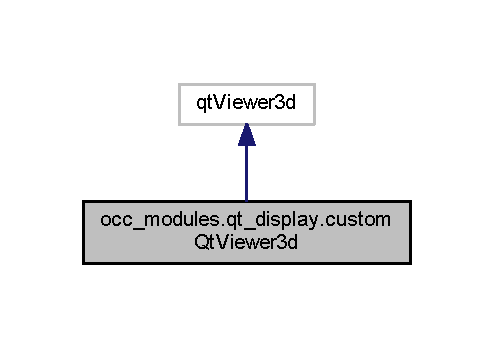
\includegraphics[width=237pt]{classocc__modules_1_1qt__display_1_1custom_qt_viewer3d__inherit__graph}
\end{center}
\end{figure}
\subsection*{Public Member Functions}
\begin{DoxyCompactItemize}
\item 
def \hyperlink{classocc__modules_1_1qt__display_1_1custom_qt_viewer3d_aeef3c40364ac364d1ffc5ba3f5122964}{\+\_\+\+\_\+init\+\_\+\+\_\+} (self, parent=None)
\item 
def \hyperlink{classocc__modules_1_1qt__display_1_1custom_qt_viewer3d_a2031b7d19b3a0c4b0f54fc90218bcdd8}{wheel\+Event} (self, event)
\begin{DoxyCompactList}\small\item\em Graphic method of the qt\+Viewer3d of python\+O\+CC that attributes function to Mouse Wheel on Qt environment. \end{DoxyCompactList}\end{DoxyCompactItemize}


\subsection{Detailed Description}
Customized class from O\+C\+C.\+Display.\+qt\+Display.\+qt\+Viewer3d of Python\+O\+CC, inheriting it and defining a new one. 

This costumized class allows to change de zoom step of mouse wheel event on Qt environment. 

\subsection{Constructor \& Destructor Documentation}
\hypertarget{classocc__modules_1_1qt__display_1_1custom_qt_viewer3d_aeef3c40364ac364d1ffc5ba3f5122964}{}\label{classocc__modules_1_1qt__display_1_1custom_qt_viewer3d_aeef3c40364ac364d1ffc5ba3f5122964} 
\index{occ\+\_\+modules\+::qt\+\_\+display\+::custom\+Qt\+Viewer3d@{occ\+\_\+modules\+::qt\+\_\+display\+::custom\+Qt\+Viewer3d}!\+\_\+\+\_\+init\+\_\+\+\_\+@{\+\_\+\+\_\+init\+\_\+\+\_\+}}
\index{\+\_\+\+\_\+init\+\_\+\+\_\+@{\+\_\+\+\_\+init\+\_\+\+\_\+}!occ\+\_\+modules\+::qt\+\_\+display\+::custom\+Qt\+Viewer3d@{occ\+\_\+modules\+::qt\+\_\+display\+::custom\+Qt\+Viewer3d}}
\subsubsection{\texorpdfstring{\+\_\+\+\_\+init\+\_\+\+\_\+()}{\_\_init\_\_()}}
{\footnotesize\ttfamily def occ\+\_\+modules.\+qt\+\_\+display.\+custom\+Qt\+Viewer3d.\+\_\+\+\_\+init\+\_\+\+\_\+ (\begin{DoxyParamCaption}\item[{}]{self,  }\item[{}]{parent = {\ttfamily None} }\end{DoxyParamCaption})}



\subsection{Member Function Documentation}
\hypertarget{classocc__modules_1_1qt__display_1_1custom_qt_viewer3d_a2031b7d19b3a0c4b0f54fc90218bcdd8}{}\label{classocc__modules_1_1qt__display_1_1custom_qt_viewer3d_a2031b7d19b3a0c4b0f54fc90218bcdd8} 
\index{occ\+\_\+modules\+::qt\+\_\+display\+::custom\+Qt\+Viewer3d@{occ\+\_\+modules\+::qt\+\_\+display\+::custom\+Qt\+Viewer3d}!wheel\+Event@{wheel\+Event}}
\index{wheel\+Event@{wheel\+Event}!occ\+\_\+modules\+::qt\+\_\+display\+::custom\+Qt\+Viewer3d@{occ\+\_\+modules\+::qt\+\_\+display\+::custom\+Qt\+Viewer3d}}
\subsubsection{\texorpdfstring{wheel\+Event()}{wheelEvent()}}
{\footnotesize\ttfamily def occ\+\_\+modules.\+qt\+\_\+display.\+custom\+Qt\+Viewer3d.\+wheel\+Event (\begin{DoxyParamCaption}\item[{}]{self,  }\item[{}]{event }\end{DoxyParamCaption})}



Graphic method of the qt\+Viewer3d of python\+O\+CC that attributes function to Mouse Wheel on Qt environment. 


\begin{DoxyParams}{Parameters}
{\em event} & \mbox{[}Qt\+Gui.\+Q\+Wheel\+Event\mbox{]} Object created triggered by user Mouse Wheel movement. \\
\hline
\end{DoxyParams}
\begin{DoxyReturn}{Returns}
None 
\end{DoxyReturn}


The documentation for this class was generated from the following file\+:\begin{DoxyCompactItemize}
\item 
\hyperlink{qt__display_8py}{qt\+\_\+display.\+py}\end{DoxyCompactItemize}

\hypertarget{classbladepro__modules_1_1inputfile__writer_1_1_input_writer_window}{}\section{bladepro\+\_\+modules.\+inputfile\+\_\+writer.\+Input\+Writer\+Window Class Reference}
\label{classbladepro__modules_1_1inputfile__writer_1_1_input_writer_window}\index{bladepro\+\_\+modules.\+inputfile\+\_\+writer.\+Input\+Writer\+Window@{bladepro\+\_\+modules.\+inputfile\+\_\+writer.\+Input\+Writer\+Window}}


Class for creating a G\+UI for the Blade\+Py Inputfile Writer Widget.  




Inheritance diagram for bladepro\+\_\+modules.\+inputfile\+\_\+writer.\+Input\+Writer\+Window\+:\nopagebreak
\begin{figure}[H]
\begin{center}
\leavevmode
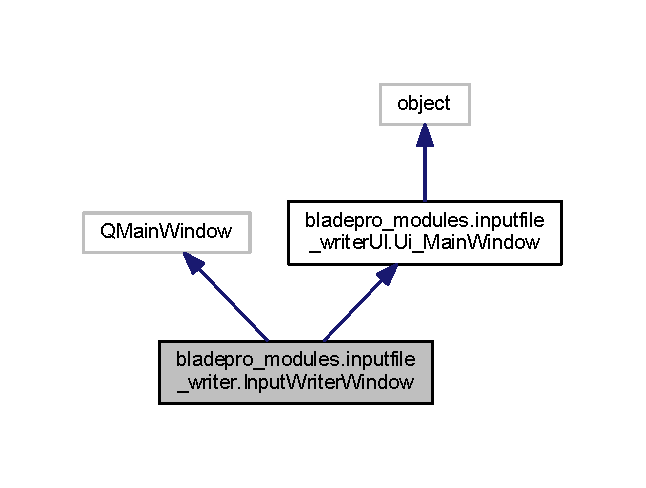
\includegraphics[width=310pt]{classbladepro__modules_1_1inputfile__writer_1_1_input_writer_window__inherit__graph}
\end{center}
\end{figure}
\subsection*{Public Member Functions}
\begin{DoxyCompactItemize}
\item 
def \hyperlink{classbladepro__modules_1_1inputfile__writer_1_1_input_writer_window_a8b9718669dac6016ebe4e4f27421c7f2}{\+\_\+\+\_\+init\+\_\+\+\_\+} (self, parent=None, Output\+Viewer\+Widget=None)
\item 
def \hyperlink{classbladepro__modules_1_1inputfile__writer_1_1_input_writer_window_a15eb2b878a78d644c96b19a5785d5428}{select\+Path} (self)
\begin{DoxyCompactList}\small\item\em Method accessed by select path button. \end{DoxyCompactList}\item 
def \hyperlink{classbladepro__modules_1_1inputfile__writer_1_1_input_writer_window_a6ec74acbc44de3023188ddd8395b5b30}{generate\+Input} (self)
\begin{DoxyCompactList}\small\item\em Calls all other methods related to Blade\+Pro keywords to generate an input file. \end{DoxyCompactList}\item 
def \hyperlink{classbladepro__modules_1_1inputfile__writer_1_1_input_writer_window_a4f95b1c85e601bde79e5d4e1a526ef8b}{run\+Blade\+Pro} (self)
\item 
def \hyperlink{classbladepro__modules_1_1inputfile__writer_1_1_input_writer_window_af311095fe10adcca5237385033dfe67b}{open\+Selected\+Cases} (self)
\begin{DoxyCompactList}\small\item\em This method will display Cases selected from Input Writer Widget list. \end{DoxyCompactList}\item 
def \hyperlink{classbladepro__modules_1_1inputfile__writer_1_1_input_writer_window_a7f4b3856d4dc973878dcbfd7697018bb}{read\+Options} (self, gen\+\_\+file)
\begin{DoxyCompactList}\small\item\em This method is called for writing at the input file the type of reading, I\+BL, I\+B\+L2 or C\+F\+T-\/\+G\+EO. \end{DoxyCompactList}\item 
def \hyperlink{classbladepro__modules_1_1inputfile__writer_1_1_input_writer_window_a3b0f9f0d1af5015219f258ad0751c778}{read\+Options\+Find} (self)
\begin{DoxyCompactList}\small\item\em Method for finding geometry file of type $\ast$.cft-\/geo, $\ast$.ibl or $\ast$.fp. \end{DoxyCompactList}\item 
def \hyperlink{classbladepro__modules_1_1inputfile__writer_1_1_input_writer_window_abf54bdb00a2743fb488463ab7247b146}{define\+Blade} (self, gen\+\_\+file)
\begin{DoxyCompactList}\small\item\em \mbox{[}N\+OT I\+M\+P\+L\+E\+M\+E\+N\+T\+ED\mbox{]} \end{DoxyCompactList}\item 
def \hyperlink{classbladepro__modules_1_1inputfile__writer_1_1_input_writer_window_aa1bef88b3d57a567e44548155e7ec02f}{modify\+Scale} (self, gen\+\_\+file)
\begin{DoxyCompactList}\small\item\em This keyword will scale the geometry. \end{DoxyCompactList}\item 
def \hyperlink{classbladepro__modules_1_1inputfile__writer_1_1_input_writer_window_a52d4edd27f78b5559e6e3683c6adb3bc}{modify\+TE} (self, gen\+\_\+file)
\begin{DoxyCompactList}\small\item\em This keyword will do a milling operation on the geometry. \end{DoxyCompactList}\item 
def \hyperlink{classbladepro__modules_1_1inputfile__writer_1_1_input_writer_window_a0894116159595156b62859c796bdea1d}{modify\+T\+E\+Help} (self)
\begin{DoxyCompactList}\small\item\em Auxiliary method that displays the figures to orient the user about coordinates parameters D, Z-\/ref and Gamma. \end{DoxyCompactList}\item 
def \hyperlink{classbladepro__modules_1_1inputfile__writer_1_1_input_writer_window_a66f6209a0c4caa0ba5e25b5fd913eff5}{modify\+Streams} (self, gen\+\_\+file)
\begin{DoxyCompactList}\small\item\em This keyword will re-\/create the blade geometry based on new section profiles created on new stream surfaces. \end{DoxyCompactList}\item 
def \hyperlink{classbladepro__modules_1_1inputfile__writer_1_1_input_writer_window_af60dda179dc289691a59b52cb8ed3e70}{modify\+Streams\+Validator} (self)
\begin{DoxyCompactList}\small\item\em Auxiliary method that validates the user input in modify streams keyword. \end{DoxyCompactList}\item 
def \hyperlink{classbladepro__modules_1_1inputfile__writer_1_1_input_writer_window_ade4195a752861e46586e7b163136620f}{modify\+Streams\+Remove\+Input} (self)
\begin{DoxyCompactList}\small\item\em Auxiliary method to the modify\+Streams method to remove an item of the span positions of combobox. \end{DoxyCompactList}\item 
def \hyperlink{classbladepro__modules_1_1inputfile__writer_1_1_input_writer_window_ada62706610465b6ba0d6fe5070cdbb9c}{output\+I\+G\+S\+Surf} (self, gen\+\_\+file)
\begin{DoxyCompactList}\small\item\em This keyword for iges files outputs. \end{DoxyCompactList}\item 
def \hyperlink{classbladepro__modules_1_1inputfile__writer_1_1_input_writer_window_ae5847a1434bc82a396cebfb20911db56}{output\+I\+G\+S\+Surf\+Remove\+Rail} (self)
\begin{DoxyCompactList}\small\item\em Auxiliary function to the output\+I\+G\+S\+Surf method to remove an item of the rails combobox. \end{DoxyCompactList}\item 
def \hyperlink{classbladepro__modules_1_1inputfile__writer_1_1_input_writer_window_a394d61e8d66fde036f84746086d6c687}{output\+I\+G\+S\+Cur3d} (self, gen\+\_\+file)
\begin{DoxyCompactList}\small\item\em This keyword outputs the curves in Cartesian x-\/y-\/z space to an igs-\/file. \end{DoxyCompactList}\item 
def \hyperlink{classbladepro__modules_1_1inputfile__writer_1_1_input_writer_window_ace84b07ce1416a3535068da6baa2e7d3}{output\+I\+G\+S\+Cur2d} (self, gen\+\_\+file)
\begin{DoxyCompactList}\small\item\em This keyword outputs the blade section profiles. \end{DoxyCompactList}\item 
def \hyperlink{classbladepro__modules_1_1inputfile__writer_1_1_input_writer_window_a60dc6e0ccec5f096ee68f997079abef3}{output\+I\+G\+S\+Pnts2\+Cur} (self, gen\+\_\+file)
\begin{DoxyCompactList}\small\item\em This keyword will spline point curves given in \char`\"{}filename\char`\"{} to an igs-\/file named filename.\+cur.\+igs. \end{DoxyCompactList}\item 
def \hyperlink{classbladepro__modules_1_1inputfile__writer_1_1_input_writer_window_a07862d0aa6332b54008342a24c2e30a3}{output\+I\+G\+S\+Pnts2\+Pnts} (self, gen\+\_\+file)
\begin{DoxyCompactList}\small\item\em This keyword will create an igs-\/file for visualizing a point. \end{DoxyCompactList}\item 
def \hyperlink{classbladepro__modules_1_1inputfile__writer_1_1_input_writer_window_abfeabe3a35852a2ce2ddf16765aef7eb}{output\+Map\+Pnts} (self, gen\+\_\+file)
\begin{DoxyCompactList}\small\item\em This keyword will map a Cartesian x-\/y-\/z point set. \end{DoxyCompactList}\item 
def \hyperlink{classbladepro__modules_1_1inputfile__writer_1_1_input_writer_window_a63d4bad24ed0fab617c1676db04a67e7}{output\+Tecplot2d} (self, gen\+\_\+file)
\begin{DoxyCompactList}\small\item\em This keyword will output the blade geometry including flow path and stream curves in Tecplot format. \end{DoxyCompactList}\item 
def \hyperlink{classbladepro__modules_1_1inputfile__writer_1_1_input_writer_window_a33919a9fe9364387c8f96fa21c35d2e8}{output\+Tecplot3d} (self, gen\+\_\+file)
\begin{DoxyCompactList}\small\item\em This keyword will output the blade geometry as surfaces in Cartesian x-\/y-\/z space. \end{DoxyCompactList}\item 
def \hyperlink{classbladepro__modules_1_1inputfile__writer_1_1_input_writer_window_adb8d68c4190d41bd93a2988562f6495b}{output\+Tecplot\+Streams} (self, gen\+\_\+file)
\begin{DoxyCompactList}\small\item\em This keyword will output the stream surfaces in Tecplot format. \end{DoxyCompactList}\item 
def \hyperlink{classbladepro__modules_1_1inputfile__writer_1_1_input_writer_window_ab3fe3d49e2e140068cb5b3b25964919f}{output\+Tecplot\+C\+F\+D\+Domain\+I\+N\+TF} (self, gen\+\_\+file)
\begin{DoxyCompactList}\small\item\em \mbox{[}N\+OT I\+M\+P\+L\+E\+M\+E\+N\+T\+ED\mbox{]} \end{DoxyCompactList}\item 
def \hyperlink{classbladepro__modules_1_1inputfile__writer_1_1_input_writer_window_a735d8bff1d58f17130859af0f97dfbd7}{output\+Tecplot\+Mer\+Grid} (self, gen\+\_\+file)
\begin{DoxyCompactList}\small\item\em \mbox{[}N\+OT I\+M\+P\+L\+E\+M\+E\+N\+T\+ED\mbox{]} \end{DoxyCompactList}\item 
def \hyperlink{classbladepro__modules_1_1inputfile__writer_1_1_input_writer_window_a504ccb848106dd7a0a4148941e2ec6d9}{output\+Tecplot\+Mer\+Grid\+L\+E\+TE} (self, gen\+\_\+file)
\begin{DoxyCompactList}\small\item\em \mbox{[}N\+OT I\+M\+P\+L\+E\+M\+E\+N\+T\+ED\mbox{]} \end{DoxyCompactList}\item 
def \hyperlink{classbladepro__modules_1_1inputfile__writer_1_1_input_writer_window_a4ea4c17b862c49ad9c51398fa9d60dbc}{output\+Tecplot\+Mer\+Grid3d} (self, gen\+\_\+file)
\begin{DoxyCompactList}\small\item\em \mbox{[}N\+OT I\+M\+P\+L\+E\+M\+E\+N\+T\+ED\mbox{]} \end{DoxyCompactList}\item 
def \hyperlink{classbladepro__modules_1_1inputfile__writer_1_1_input_writer_window_ab5d0d97e4bf1dd0ddf28f4f537fea598}{output\+Camber\+Angles} (self, gen\+\_\+file)
\begin{DoxyCompactList}\small\item\em This keyword will print the camber angles (beta) for each profile section to file. \end{DoxyCompactList}\item 
def \hyperlink{classbladepro__modules_1_1inputfile__writer_1_1_input_writer_window_a9d8a631853a80acf18ab0d1c05a11dec}{output\+Sweep\+Angle} (self, gen\+\_\+file)
\begin{DoxyCompactList}\small\item\em This keyword will output a .sweep file. \end{DoxyCompactList}\item 
def \hyperlink{classbladepro__modules_1_1inputfile__writer_1_1_input_writer_window_a6dc19a2bae75b4c52b4337a55574363d}{output\+StreamC} (self, gen\+\_\+file)
\begin{DoxyCompactList}\small\item\em This keyword will write the flow path (hub \& shroud) and the stream curves to a file. \end{DoxyCompactList}\item 
def \hyperlink{classbladepro__modules_1_1inputfile__writer_1_1_input_writer_window_a38ac1495c5c1cc730241601a8300d632}{output\+Stack\+Cur} (self, gen\+\_\+file)
\begin{DoxyCompactList}\small\item\em The stacking position in selected space for each blade section will be written to a file. \end{DoxyCompactList}\item 
def \hyperlink{classbladepro__modules_1_1inputfile__writer_1_1_input_writer_window_a15fdf4aaecf99b885796124500f80114}{output\+HeightV} (self, gen\+\_\+file)
\begin{DoxyCompactList}\small\item\em This keyword will write the streamtube height variation for n points on each stream curve to file. \end{DoxyCompactList}\item 
def \hyperlink{classbladepro__modules_1_1inputfile__writer_1_1_input_writer_window_af96b8ec5130403c737d4105e04edea5d}{output\+T\+E\+Pos} (self, gen\+\_\+file)
\begin{DoxyCompactList}\small\item\em Write the trailing edge position of each blade section in cylindrical r-\/teta-\/z space to a file. \end{DoxyCompactList}\item 
def \hyperlink{classbladepro__modules_1_1inputfile__writer_1_1_input_writer_window_a93fdb47e6f9162ce3fe7ef624f7681aa}{output\+T\+E\+Cur} (self, gen\+\_\+file)
\begin{DoxyCompactList}\small\item\em Write trailing edge point curve in meridional plane to a file with n points. \end{DoxyCompactList}\item 
def \hyperlink{classbladepro__modules_1_1inputfile__writer_1_1_input_writer_window_a55ddee4c839782858d6f53a49b9c63ec}{output\+L\+E\+Cur} (self, gen\+\_\+file)
\begin{DoxyCompactList}\small\item\em Write leading edge point curve in meridional plane to a file with n points. \end{DoxyCompactList}\item 
def \hyperlink{classbladepro__modules_1_1inputfile__writer_1_1_input_writer_window_a27407b1e60e56fceec34147b9b793a74}{output\+R\+T\+ZT} (self, gen\+\_\+file)
\begin{DoxyCompactList}\small\item\em This keyword will export the geometry to Blade\+Modeler rtzt-\/format from A\+N\+S\+YS. \end{DoxyCompactList}\item 
def \hyperlink{classbladepro__modules_1_1inputfile__writer_1_1_input_writer_window_ad727ca92f2959a8d915939c73f3dbff1}{output\+C\+FT} (self, gen\+\_\+file)
\begin{DoxyCompactList}\small\item\em This keyword will create a C\+Fturbo project file (version 10.\+1) of a radial impeller geometry. \end{DoxyCompactList}\item 
def \hyperlink{classbladepro__modules_1_1inputfile__writer_1_1_input_writer_window_a61f9db1d33a2cb583c3f779a94ec700d}{output\+Auto\+Grid} (self, gen\+\_\+file)
\begin{DoxyCompactList}\small\item\em This keyword will create a Numeca .geom\+Turbo file. \end{DoxyCompactList}\item 
def \hyperlink{classbladepro__modules_1_1inputfile__writer_1_1_input_writer_window_aa7a1b9b7db9021015b02a691075d88e3}{output\+I\+G\+S\+C\+F\+D\+Domain\+P2P} (self, gen\+\_\+file)
\begin{DoxyCompactList}\small\item\em \mbox{[}N\+OT I\+M\+P\+L\+E\+M\+E\+N\+T\+ED\mbox{]} \end{DoxyCompactList}\item 
def \hyperlink{classbladepro__modules_1_1inputfile__writer_1_1_input_writer_window_a8e556016279f9aabdabb9b6f708c95cb}{output\+I\+G\+S\+C\+F\+D\+Domain\+B2B} (self, gen\+\_\+file)
\begin{DoxyCompactList}\small\item\em \mbox{[}N\+OT I\+M\+P\+L\+E\+M\+E\+N\+T\+ED\mbox{]} \end{DoxyCompactList}\item 
def \hyperlink{classbladepro__modules_1_1inputfile__writer_1_1_input_writer_window_a1a577ed1880def26fc13d02701e9346a}{output\+I\+G\+S\+C\+F\+D\+Domain\+Inlet} (self, gen\+\_\+file)
\begin{DoxyCompactList}\small\item\em \mbox{[}N\+OT I\+M\+P\+L\+E\+M\+E\+N\+T\+ED\mbox{]} \end{DoxyCompactList}\item 
def \hyperlink{classbladepro__modules_1_1inputfile__writer_1_1_input_writer_window_aa16a1dab2d93130c1cc0b4c24ec2caef}{output\+I\+G\+S\+C\+F\+D\+Domain\+I\+N\+TF} (self, gen\+\_\+file)
\begin{DoxyCompactList}\small\item\em \mbox{[}N\+OT I\+M\+P\+L\+E\+M\+E\+N\+T\+ED\mbox{]} \end{DoxyCompactList}\item 
def \hyperlink{classbladepro__modules_1_1inputfile__writer_1_1_input_writer_window_a3093ea91273711f4b82aa878c0204407}{output\+I\+G\+S\+C\+F\+D\+Domain\+Periodic} (self, gen\+\_\+file)
\begin{DoxyCompactList}\small\item\em \mbox{[}N\+OT I\+M\+P\+L\+E\+M\+E\+N\+T\+ED\mbox{]} \end{DoxyCompactList}\item 
def \hyperlink{classbladepro__modules_1_1inputfile__writer_1_1_input_writer_window_a3b5fc7f417d1912f563df69560f57c2e}{output\+Cur\+C\+F\+D\+Domain\+P2P} (self, gen\+\_\+file)
\begin{DoxyCompactList}\small\item\em \mbox{[}N\+OT I\+M\+P\+L\+E\+M\+E\+N\+T\+ED\mbox{]} \end{DoxyCompactList}\item 
def \hyperlink{classbladepro__modules_1_1inputfile__writer_1_1_input_writer_window_a925f588daf72fce3ec4e0b89839c290d}{output\+Cur\+C\+F\+D\+Domain\+B2B} (self, gen\+\_\+file)
\begin{DoxyCompactList}\small\item\em \mbox{[}N\+OT I\+M\+P\+L\+E\+M\+E\+N\+T\+ED\mbox{]} \end{DoxyCompactList}\item 
def \hyperlink{classbladepro__modules_1_1inputfile__writer_1_1_input_writer_window_a998cb328088bc95e267cffed35c231ce}{output\+Gmsh\+C\+F\+D\+Domain\+P2P} (self, gen\+\_\+file)
\begin{DoxyCompactList}\small\item\em \mbox{[}N\+OT I\+M\+P\+L\+E\+M\+E\+N\+T\+ED\mbox{]} \end{DoxyCompactList}\item 
def \hyperlink{classbladepro__modules_1_1inputfile__writer_1_1_input_writer_window_a0044216044b48baae08e478a2f358c39}{output\+Gmsh\+Mer\+Grid} (self, gen\+\_\+file)
\begin{DoxyCompactList}\small\item\em \mbox{[}N\+OT I\+M\+P\+L\+E\+M\+E\+N\+T\+ED\mbox{]} \end{DoxyCompactList}\item 
def \hyperlink{classbladepro__modules_1_1inputfile__writer_1_1_input_writer_window_a36211b3ff2243e25921e48d71b9dcf7c}{output\+Gmsh\+Mer\+Grid\+L\+E\+TE} (self, gen\+\_\+file)
\begin{DoxyCompactList}\small\item\em \mbox{[}N\+OT I\+M\+P\+L\+E\+M\+E\+N\+T\+ED\mbox{]} \end{DoxyCompactList}\item 
def \hyperlink{classbladepro__modules_1_1inputfile__writer_1_1_input_writer_window_a258f943645c60945cbb97494db0ebf52}{output\+Gmsh\+Inp\+Mer\+Grid} (self, gen\+\_\+file)
\begin{DoxyCompactList}\small\item\em \mbox{[}N\+OT I\+M\+P\+L\+E\+M\+E\+N\+T\+ED\mbox{]} \end{DoxyCompactList}\item 
def \hyperlink{classbladepro__modules_1_1inputfile__writer_1_1_input_writer_window_aa07573686af3bd04e4ff42c3dddcf975}{output\+Gmsh\+Inp\+Mer\+Grid\+L\+E\+TE} (self, gen\+\_\+file)
\begin{DoxyCompactList}\small\item\em \mbox{[}N\+OT I\+M\+P\+L\+E\+M\+E\+N\+T\+ED\mbox{]} \end{DoxyCompactList}\item 
def \hyperlink{classbladepro__modules_1_1inputfile__writer_1_1_input_writer_window_a464a8ac16bcb67d41a6d91ee8b51acf2}{rename\+Setting} (self)
\begin{DoxyCompactList}\small\item\em Renames the name of user defined settings to make their name represent something to the user. \end{DoxyCompactList}\item 
def \hyperlink{classbladepro__modules_1_1inputfile__writer_1_1_input_writer_window_a35cf87c6230239ce47b33bda03bd7432}{menu\+File\+Button\+Pressed\+Group} (self, pressed\+\_\+btn)
\begin{DoxyCompactList}\small\item\em Method group that wrap only exit function for \char`\"{}file\char`\"{} menu. \end{DoxyCompactList}\item 
def \hyperlink{classbladepro__modules_1_1inputfile__writer_1_1_input_writer_window_ad94f49b4827a3ea0b56070e0149ae2aa}{menu\+File\+Bladepro\+Button\+Pressed\+Group} (self, pressed\+\_\+btn)
\begin{DoxyCompactList}\small\item\em Method group that wrap all functions for File and Blade\+Pro buttons in toolbar. \end{DoxyCompactList}\item 
def \hyperlink{classbladepro__modules_1_1inputfile__writer_1_1_input_writer_window_a1b508dd4cb9c699a1769e7727d1e6fc1}{user\+Settings\+Button\+Pressed\+Group} (self, button\+\_\+pressed)
\begin{DoxyCompactList}\small\item\em Method group that wrap all functions for user settings options in toolbar. \end{DoxyCompactList}\item 
def \hyperlink{classbladepro__modules_1_1inputfile__writer_1_1_input_writer_window_a0c4f30850537553db0ff2e27059733a4}{load\+Settings} (self, setting)
\begin{DoxyCompactList}\small\item\em Loads the user settings defined in \char`\"{}setting\char`\"{} index. \end{DoxyCompactList}\item 
def \hyperlink{classbladepro__modules_1_1inputfile__writer_1_1_input_writer_window_a0e71786a8b6fe43e6a01ff388c34ce18}{quick\+List\+Function} (self)
\begin{DoxyCompactList}\small\item\em Enables list of settings quick navigation. \end{DoxyCompactList}\item 
def \hyperlink{classbladepro__modules_1_1inputfile__writer_1_1_input_writer_window_a723573fade09f206a9c89569885558c1}{save\+Settings} (self, setting)
\begin{DoxyCompactList}\small\item\em Save the settings defined in \char`\"{}setting\char`\"{} index. \end{DoxyCompactList}\end{DoxyCompactItemize}
\subsection*{Public Attributes}
\begin{DoxyCompactItemize}
\item 
\hyperlink{classbladepro__modules_1_1inputfile__writer_1_1_input_writer_window_ad019b7f076cb8b8b6820b6577d2058b6}{list\+\_\+settings}
\item 
\hyperlink{classbladepro__modules_1_1inputfile__writer_1_1_input_writer_window_a17d54af05f4344118b082c2384a88bec}{file\+\_\+geometry}
\item 
\hyperlink{classbladepro__modules_1_1inputfile__writer_1_1_input_writer_window_a267e018648a6f03f2bcc0a5b7c944f38}{working\+\_\+directory}
\item 
\hyperlink{classbladepro__modules_1_1inputfile__writer_1_1_input_writer_window_a4f8dfa192201c6c945621ff197680200}{user\+\_\+settings}
\item 
\hyperlink{classbladepro__modules_1_1inputfile__writer_1_1_input_writer_window_aa8731441bd4fdf801f74947c28d44ebf}{last\+\_\+settings}
\item 
\hyperlink{classbladepro__modules_1_1inputfile__writer_1_1_input_writer_window_a3ce7139eaa5256714413efdb9f870eab}{settings\+\_\+names}
\item 
\hyperlink{classbladepro__modules_1_1inputfile__writer_1_1_input_writer_window_af3daf3ca641b77de41d08750af03ef5e}{op\+\_\+viewer}
\item 
\hyperlink{classbladepro__modules_1_1inputfile__writer_1_1_input_writer_window_aa6e2504eda6ac2ee99e37d4b5f862f57}{no\+\_\+validator}
\item 
\hyperlink{classbladepro__modules_1_1inputfile__writer_1_1_input_writer_window_a33d2c6ecfa0800ef5eccfe0ce71475ee}{integer\+\_\+validator}
\item 
\hyperlink{classbladepro__modules_1_1inputfile__writer_1_1_input_writer_window_a007df19a104366a8bb63a8ed11e0e5e4}{double\+\_\+validator}
\item 
\hyperlink{classbladepro__modules_1_1inputfile__writer_1_1_input_writer_window_a2e8a633f45ef3a17852bc95deae51588}{working\+\_\+path}
\end{DoxyCompactItemize}


\subsection{Detailed Description}
Class for creating a G\+UI for the Blade\+Py Inputfile Writer Widget. 

This class inherits the \hyperlink{classbladepro__modules_1_1inputfile__writer_u_i_1_1_ui___main_window}{inputfile\+\_\+writer\+U\+I.\+Ui\+\_\+\+Main\+Window}, the layout created in Qt Designer. This class has methods for generating the inputfiles for running Blade\+Pro. Clicking the checkboxes enables the usage of the keywords.

The class can hold up to 10 different User Preferences that can be named any name the user wants. The User Preferences are managed by \hyperlink{classbladepro__modules_1_1inputfile__writer_1_1_input_writer_window_a0c4f30850537553db0ff2e27059733a4}{load\+Settings()} and \hyperlink{classbladepro__modules_1_1inputfile__writer_1_1_input_writer_window_a723573fade09f206a9c89569885558c1}{save\+Settings()} methods 

\subsection{Constructor \& Destructor Documentation}
\hypertarget{classbladepro__modules_1_1inputfile__writer_1_1_input_writer_window_a8b9718669dac6016ebe4e4f27421c7f2}{}\label{classbladepro__modules_1_1inputfile__writer_1_1_input_writer_window_a8b9718669dac6016ebe4e4f27421c7f2} 
\index{bladepro\+\_\+modules\+::inputfile\+\_\+writer\+::\+Input\+Writer\+Window@{bladepro\+\_\+modules\+::inputfile\+\_\+writer\+::\+Input\+Writer\+Window}!\+\_\+\+\_\+init\+\_\+\+\_\+@{\+\_\+\+\_\+init\+\_\+\+\_\+}}
\index{\+\_\+\+\_\+init\+\_\+\+\_\+@{\+\_\+\+\_\+init\+\_\+\+\_\+}!bladepro\+\_\+modules\+::inputfile\+\_\+writer\+::\+Input\+Writer\+Window@{bladepro\+\_\+modules\+::inputfile\+\_\+writer\+::\+Input\+Writer\+Window}}
\subsubsection{\texorpdfstring{\+\_\+\+\_\+init\+\_\+\+\_\+()}{\_\_init\_\_()}}
{\footnotesize\ttfamily def bladepro\+\_\+modules.\+inputfile\+\_\+writer.\+Input\+Writer\+Window.\+\_\+\+\_\+init\+\_\+\+\_\+ (\begin{DoxyParamCaption}\item[{}]{self,  }\item[{}]{parent = {\ttfamily None},  }\item[{}]{Output\+Viewer\+Widget = {\ttfamily None} }\end{DoxyParamCaption})}



\subsection{Member Function Documentation}
\hypertarget{classbladepro__modules_1_1inputfile__writer_1_1_input_writer_window_abf54bdb00a2743fb488463ab7247b146}{}\label{classbladepro__modules_1_1inputfile__writer_1_1_input_writer_window_abf54bdb00a2743fb488463ab7247b146} 
\index{bladepro\+\_\+modules\+::inputfile\+\_\+writer\+::\+Input\+Writer\+Window@{bladepro\+\_\+modules\+::inputfile\+\_\+writer\+::\+Input\+Writer\+Window}!define\+Blade@{define\+Blade}}
\index{define\+Blade@{define\+Blade}!bladepro\+\_\+modules\+::inputfile\+\_\+writer\+::\+Input\+Writer\+Window@{bladepro\+\_\+modules\+::inputfile\+\_\+writer\+::\+Input\+Writer\+Window}}
\subsubsection{\texorpdfstring{define\+Blade()}{defineBlade()}}
{\footnotesize\ttfamily def bladepro\+\_\+modules.\+inputfile\+\_\+writer.\+Input\+Writer\+Window.\+define\+Blade (\begin{DoxyParamCaption}\item[{}]{self,  }\item[{}]{gen\+\_\+file }\end{DoxyParamCaption})}



\mbox{[}N\+OT I\+M\+P\+L\+E\+M\+E\+N\+T\+ED\mbox{]} 


\begin{DoxyParams}{Parameters}
{\em gen\+\_\+file} & \mbox{[}txt\mbox{]} Is the file to what the new lines are being saved to. \\
\hline
\end{DoxyParams}
\begin{DoxyReturn}{Returns}
None 
\end{DoxyReturn}
\hypertarget{classbladepro__modules_1_1inputfile__writer_1_1_input_writer_window_a6ec74acbc44de3023188ddd8395b5b30}{}\label{classbladepro__modules_1_1inputfile__writer_1_1_input_writer_window_a6ec74acbc44de3023188ddd8395b5b30} 
\index{bladepro\+\_\+modules\+::inputfile\+\_\+writer\+::\+Input\+Writer\+Window@{bladepro\+\_\+modules\+::inputfile\+\_\+writer\+::\+Input\+Writer\+Window}!generate\+Input@{generate\+Input}}
\index{generate\+Input@{generate\+Input}!bladepro\+\_\+modules\+::inputfile\+\_\+writer\+::\+Input\+Writer\+Window@{bladepro\+\_\+modules\+::inputfile\+\_\+writer\+::\+Input\+Writer\+Window}}
\subsubsection{\texorpdfstring{generate\+Input()}{generateInput()}}
{\footnotesize\ttfamily def bladepro\+\_\+modules.\+inputfile\+\_\+writer.\+Input\+Writer\+Window.\+generate\+Input (\begin{DoxyParamCaption}\item[{}]{self }\end{DoxyParamCaption})}



Calls all other methods related to Blade\+Pro keywords to generate an input file. 

This method is called by ui\+\_\+button press or after loading any user settings. It calls all keywords methods of Blade\+Pro independent if they are going to generate something.

\begin{DoxyReturn}{Returns}
None 
\end{DoxyReturn}
\hypertarget{classbladepro__modules_1_1inputfile__writer_1_1_input_writer_window_a0c4f30850537553db0ff2e27059733a4}{}\label{classbladepro__modules_1_1inputfile__writer_1_1_input_writer_window_a0c4f30850537553db0ff2e27059733a4} 
\index{bladepro\+\_\+modules\+::inputfile\+\_\+writer\+::\+Input\+Writer\+Window@{bladepro\+\_\+modules\+::inputfile\+\_\+writer\+::\+Input\+Writer\+Window}!load\+Settings@{load\+Settings}}
\index{load\+Settings@{load\+Settings}!bladepro\+\_\+modules\+::inputfile\+\_\+writer\+::\+Input\+Writer\+Window@{bladepro\+\_\+modules\+::inputfile\+\_\+writer\+::\+Input\+Writer\+Window}}
\subsubsection{\texorpdfstring{load\+Settings()}{loadSettings()}}
{\footnotesize\ttfamily def bladepro\+\_\+modules.\+inputfile\+\_\+writer.\+Input\+Writer\+Window.\+load\+Settings (\begin{DoxyParamCaption}\item[{}]{self,  }\item[{}]{setting }\end{DoxyParamCaption})}



Loads the user settings defined in \char`\"{}setting\char`\"{} index. 

This will check all checkboxes and modify all the fields according to the setting loaded.

The last user settings is defined by setting = -\/1. Thus, to load last user settings the function call is load\+Settings(-\/1). There is up to 10 sets available, starting with setting = 0.


\begin{DoxyParams}{Parameters}
{\em setting} & \mbox{[}int\mbox{]} Is the ui\+\_\+listsettings\+\_\+combo index. \\
\hline
\end{DoxyParams}
\begin{DoxyReturn}{Returns}
None 
\end{DoxyReturn}
\hypertarget{classbladepro__modules_1_1inputfile__writer_1_1_input_writer_window_ad94f49b4827a3ea0b56070e0149ae2aa}{}\label{classbladepro__modules_1_1inputfile__writer_1_1_input_writer_window_ad94f49b4827a3ea0b56070e0149ae2aa} 
\index{bladepro\+\_\+modules\+::inputfile\+\_\+writer\+::\+Input\+Writer\+Window@{bladepro\+\_\+modules\+::inputfile\+\_\+writer\+::\+Input\+Writer\+Window}!menu\+File\+Bladepro\+Button\+Pressed\+Group@{menu\+File\+Bladepro\+Button\+Pressed\+Group}}
\index{menu\+File\+Bladepro\+Button\+Pressed\+Group@{menu\+File\+Bladepro\+Button\+Pressed\+Group}!bladepro\+\_\+modules\+::inputfile\+\_\+writer\+::\+Input\+Writer\+Window@{bladepro\+\_\+modules\+::inputfile\+\_\+writer\+::\+Input\+Writer\+Window}}
\subsubsection{\texorpdfstring{menu\+File\+Bladepro\+Button\+Pressed\+Group()}{menuFileBladeproButtonPressedGroup()}}
{\footnotesize\ttfamily def bladepro\+\_\+modules.\+inputfile\+\_\+writer.\+Input\+Writer\+Window.\+menu\+File\+Bladepro\+Button\+Pressed\+Group (\begin{DoxyParamCaption}\item[{}]{self,  }\item[{}]{pressed\+\_\+btn }\end{DoxyParamCaption})}



Method group that wrap all functions for File and Blade\+Pro buttons in toolbar. 


\begin{DoxyParams}{Parameters}
{\em pressed\+\_\+btn} & \mbox{[}Qt\+Gui.\+Q\+Action\mbox{]} Signal emitted by button clicked on ui\+\_\+bladepro\+\_\+toolbar \\
\hline
\end{DoxyParams}
\begin{DoxyReturn}{Returns}
None 
\end{DoxyReturn}
\hypertarget{classbladepro__modules_1_1inputfile__writer_1_1_input_writer_window_a35cf87c6230239ce47b33bda03bd7432}{}\label{classbladepro__modules_1_1inputfile__writer_1_1_input_writer_window_a35cf87c6230239ce47b33bda03bd7432} 
\index{bladepro\+\_\+modules\+::inputfile\+\_\+writer\+::\+Input\+Writer\+Window@{bladepro\+\_\+modules\+::inputfile\+\_\+writer\+::\+Input\+Writer\+Window}!menu\+File\+Button\+Pressed\+Group@{menu\+File\+Button\+Pressed\+Group}}
\index{menu\+File\+Button\+Pressed\+Group@{menu\+File\+Button\+Pressed\+Group}!bladepro\+\_\+modules\+::inputfile\+\_\+writer\+::\+Input\+Writer\+Window@{bladepro\+\_\+modules\+::inputfile\+\_\+writer\+::\+Input\+Writer\+Window}}
\subsubsection{\texorpdfstring{menu\+File\+Button\+Pressed\+Group()}{menuFileButtonPressedGroup()}}
{\footnotesize\ttfamily def bladepro\+\_\+modules.\+inputfile\+\_\+writer.\+Input\+Writer\+Window.\+menu\+File\+Button\+Pressed\+Group (\begin{DoxyParamCaption}\item[{}]{self,  }\item[{}]{pressed\+\_\+btn }\end{DoxyParamCaption})}



Method group that wrap only exit function for \char`\"{}file\char`\"{} menu. 

The others are wrapped in the toolbar pressed group \begin{DoxyVerb}   @param pressed_btn [QtGui.QAction] Signal emitted by button clicked on ui_file_menur
   @return None\end{DoxyVerb}
 \hypertarget{classbladepro__modules_1_1inputfile__writer_1_1_input_writer_window_aa1bef88b3d57a567e44548155e7ec02f}{}\label{classbladepro__modules_1_1inputfile__writer_1_1_input_writer_window_aa1bef88b3d57a567e44548155e7ec02f} 
\index{bladepro\+\_\+modules\+::inputfile\+\_\+writer\+::\+Input\+Writer\+Window@{bladepro\+\_\+modules\+::inputfile\+\_\+writer\+::\+Input\+Writer\+Window}!modify\+Scale@{modify\+Scale}}
\index{modify\+Scale@{modify\+Scale}!bladepro\+\_\+modules\+::inputfile\+\_\+writer\+::\+Input\+Writer\+Window@{bladepro\+\_\+modules\+::inputfile\+\_\+writer\+::\+Input\+Writer\+Window}}
\subsubsection{\texorpdfstring{modify\+Scale()}{modifyScale()}}
{\footnotesize\ttfamily def bladepro\+\_\+modules.\+inputfile\+\_\+writer.\+Input\+Writer\+Window.\+modify\+Scale (\begin{DoxyParamCaption}\item[{}]{self,  }\item[{}]{gen\+\_\+file }\end{DoxyParamCaption})}



This keyword will scale the geometry. 

This keyword will scale the geometry with the vector valued scale factor f = (x-\/sc, y-\/sc, z-\/sc) with respect to a point C = (xc, yc, zc).


\begin{DoxyParams}{Parameters}
{\em gen\+\_\+file} & \mbox{[}txt\mbox{]} Is the file to what the new lines are being saved to. \\
\hline
\end{DoxyParams}
\begin{DoxyReturn}{Returns}
None 
\end{DoxyReturn}
\hypertarget{classbladepro__modules_1_1inputfile__writer_1_1_input_writer_window_a66f6209a0c4caa0ba5e25b5fd913eff5}{}\label{classbladepro__modules_1_1inputfile__writer_1_1_input_writer_window_a66f6209a0c4caa0ba5e25b5fd913eff5} 
\index{bladepro\+\_\+modules\+::inputfile\+\_\+writer\+::\+Input\+Writer\+Window@{bladepro\+\_\+modules\+::inputfile\+\_\+writer\+::\+Input\+Writer\+Window}!modify\+Streams@{modify\+Streams}}
\index{modify\+Streams@{modify\+Streams}!bladepro\+\_\+modules\+::inputfile\+\_\+writer\+::\+Input\+Writer\+Window@{bladepro\+\_\+modules\+::inputfile\+\_\+writer\+::\+Input\+Writer\+Window}}
\subsubsection{\texorpdfstring{modify\+Streams()}{modifyStreams()}}
{\footnotesize\ttfamily def bladepro\+\_\+modules.\+inputfile\+\_\+writer.\+Input\+Writer\+Window.\+modify\+Streams (\begin{DoxyParamCaption}\item[{}]{self,  }\item[{}]{gen\+\_\+file }\end{DoxyParamCaption})}



This keyword will re-\/create the blade geometry based on new section profiles created on new stream surfaces. 

The new stream surfaces can be specified in three different ways by method\+:

\begin{DoxyItemize}
\item {\ttfamily E\+L\+L\+I\+P\+T\+IC\+:} constant span positions based on elliptic grid \item {\ttfamily O\+R\+T\+H\+O\+G\+O\+N\+AL\+:} constant span positions based on orthogonal grid \item {\ttfamily F\+I\+LE\+:} arbitrary stream surfaces read from file.\end{DoxyItemize}
The elliptic option will create the new stream surfaces on equally spaced span position where the user specifies the number of stream surfaces

The orthogonal option lets the user specify the interior span positions, i.\+e. 0 $<$ span $<$ 1. Stream surfaces at hub (span = 0) and shroud (span = 1) will automatically be created so the total number of stream surfaces will then be n + 2.

The file option reads the interior stream surfaces (stream surfaces at hub and shroud will automatically be created like the elliptic option)


\begin{DoxyParams}{Parameters}
{\em gen\+\_\+file} & \mbox{[}txt\mbox{]} Is the file to what the new lines are being saved to. \\
\hline
\end{DoxyParams}
\begin{DoxyReturn}{Returns}
None 
\end{DoxyReturn}
\hypertarget{classbladepro__modules_1_1inputfile__writer_1_1_input_writer_window_ade4195a752861e46586e7b163136620f}{}\label{classbladepro__modules_1_1inputfile__writer_1_1_input_writer_window_ade4195a752861e46586e7b163136620f} 
\index{bladepro\+\_\+modules\+::inputfile\+\_\+writer\+::\+Input\+Writer\+Window@{bladepro\+\_\+modules\+::inputfile\+\_\+writer\+::\+Input\+Writer\+Window}!modify\+Streams\+Remove\+Input@{modify\+Streams\+Remove\+Input}}
\index{modify\+Streams\+Remove\+Input@{modify\+Streams\+Remove\+Input}!bladepro\+\_\+modules\+::inputfile\+\_\+writer\+::\+Input\+Writer\+Window@{bladepro\+\_\+modules\+::inputfile\+\_\+writer\+::\+Input\+Writer\+Window}}
\subsubsection{\texorpdfstring{modify\+Streams\+Remove\+Input()}{modifyStreamsRemoveInput()}}
{\footnotesize\ttfamily def bladepro\+\_\+modules.\+inputfile\+\_\+writer.\+Input\+Writer\+Window.\+modify\+Streams\+Remove\+Input (\begin{DoxyParamCaption}\item[{}]{self }\end{DoxyParamCaption})}



Auxiliary method to the modify\+Streams method to remove an item of the span positions of combobox. 

\begin{DoxyReturn}{Returns}
None 
\end{DoxyReturn}
\hypertarget{classbladepro__modules_1_1inputfile__writer_1_1_input_writer_window_af60dda179dc289691a59b52cb8ed3e70}{}\label{classbladepro__modules_1_1inputfile__writer_1_1_input_writer_window_af60dda179dc289691a59b52cb8ed3e70} 
\index{bladepro\+\_\+modules\+::inputfile\+\_\+writer\+::\+Input\+Writer\+Window@{bladepro\+\_\+modules\+::inputfile\+\_\+writer\+::\+Input\+Writer\+Window}!modify\+Streams\+Validator@{modify\+Streams\+Validator}}
\index{modify\+Streams\+Validator@{modify\+Streams\+Validator}!bladepro\+\_\+modules\+::inputfile\+\_\+writer\+::\+Input\+Writer\+Window@{bladepro\+\_\+modules\+::inputfile\+\_\+writer\+::\+Input\+Writer\+Window}}
\subsubsection{\texorpdfstring{modify\+Streams\+Validator()}{modifyStreamsValidator()}}
{\footnotesize\ttfamily def bladepro\+\_\+modules.\+inputfile\+\_\+writer.\+Input\+Writer\+Window.\+modify\+Streams\+Validator (\begin{DoxyParamCaption}\item[{}]{self }\end{DoxyParamCaption})}



Auxiliary method that validates the user input in modify streams keyword. 

This method is called by signal-\/slot system. When the ui\+\_\+modify\+\_\+streams\+\_\+opt\+\_\+combo combobox item is changed, this method is activated. The arguments accepted by each case are\+:

\begin{DoxyItemize}
\item {\ttfamily E\+L\+L\+I\+P\+T\+IC\+:} the argument is a single integer \item {\ttfamily O\+R\+T\+H\+O\+G\+O\+N\+AL\+:} the argument can be a list of doubles \item {\ttfamily F\+I\+LE\+:} the argument is a single file\end{DoxyItemize}
\begin{DoxyReturn}{Returns}
None 
\end{DoxyReturn}
\hypertarget{classbladepro__modules_1_1inputfile__writer_1_1_input_writer_window_a52d4edd27f78b5559e6e3683c6adb3bc}{}\label{classbladepro__modules_1_1inputfile__writer_1_1_input_writer_window_a52d4edd27f78b5559e6e3683c6adb3bc} 
\index{bladepro\+\_\+modules\+::inputfile\+\_\+writer\+::\+Input\+Writer\+Window@{bladepro\+\_\+modules\+::inputfile\+\_\+writer\+::\+Input\+Writer\+Window}!modify\+TE@{modify\+TE}}
\index{modify\+TE@{modify\+TE}!bladepro\+\_\+modules\+::inputfile\+\_\+writer\+::\+Input\+Writer\+Window@{bladepro\+\_\+modules\+::inputfile\+\_\+writer\+::\+Input\+Writer\+Window}}
\subsubsection{\texorpdfstring{modify\+T\+E()}{modifyTE()}}
{\footnotesize\ttfamily def bladepro\+\_\+modules.\+inputfile\+\_\+writer.\+Input\+Writer\+Window.\+modify\+TE (\begin{DoxyParamCaption}\item[{}]{self,  }\item[{}]{gen\+\_\+file }\end{DoxyParamCaption})}



This keyword will do a milling operation on the geometry. 

This keyword will do a milling operation on the geometry by cutting the blade geometry with the surface of revolution created by the line in the meridional plane defined by the point (z-\/ref, D/2) with angle gamma.

There is two options in the G\+UI, modify/\+TE and modify/\+T\+E/\+I\+BL. In modify/\+T\+E/\+I\+BL diameter, z-\/reference and gamma angled are read from the ibl-\/file not from the G\+UI.


\begin{DoxyParams}{Parameters}
{\em gen\+\_\+file} & \mbox{[}txt\mbox{]} Is the file to what the new lines are being saved to. \\
\hline
\end{DoxyParams}
\begin{DoxyReturn}{Returns}
None 
\end{DoxyReturn}
\hypertarget{classbladepro__modules_1_1inputfile__writer_1_1_input_writer_window_a0894116159595156b62859c796bdea1d}{}\label{classbladepro__modules_1_1inputfile__writer_1_1_input_writer_window_a0894116159595156b62859c796bdea1d} 
\index{bladepro\+\_\+modules\+::inputfile\+\_\+writer\+::\+Input\+Writer\+Window@{bladepro\+\_\+modules\+::inputfile\+\_\+writer\+::\+Input\+Writer\+Window}!modify\+T\+E\+Help@{modify\+T\+E\+Help}}
\index{modify\+T\+E\+Help@{modify\+T\+E\+Help}!bladepro\+\_\+modules\+::inputfile\+\_\+writer\+::\+Input\+Writer\+Window@{bladepro\+\_\+modules\+::inputfile\+\_\+writer\+::\+Input\+Writer\+Window}}
\subsubsection{\texorpdfstring{modify\+T\+E\+Help()}{modifyTEHelp()}}
{\footnotesize\ttfamily def bladepro\+\_\+modules.\+inputfile\+\_\+writer.\+Input\+Writer\+Window.\+modify\+T\+E\+Help (\begin{DoxyParamCaption}\item[{}]{self }\end{DoxyParamCaption})}



Auxiliary method that displays the figures to orient the user about coordinates parameters D, Z-\/ref and Gamma. 

\begin{DoxyReturn}{Returns}
None 
\end{DoxyReturn}
\hypertarget{classbladepro__modules_1_1inputfile__writer_1_1_input_writer_window_af311095fe10adcca5237385033dfe67b}{}\label{classbladepro__modules_1_1inputfile__writer_1_1_input_writer_window_af311095fe10adcca5237385033dfe67b} 
\index{bladepro\+\_\+modules\+::inputfile\+\_\+writer\+::\+Input\+Writer\+Window@{bladepro\+\_\+modules\+::inputfile\+\_\+writer\+::\+Input\+Writer\+Window}!open\+Selected\+Cases@{open\+Selected\+Cases}}
\index{open\+Selected\+Cases@{open\+Selected\+Cases}!bladepro\+\_\+modules\+::inputfile\+\_\+writer\+::\+Input\+Writer\+Window@{bladepro\+\_\+modules\+::inputfile\+\_\+writer\+::\+Input\+Writer\+Window}}
\subsubsection{\texorpdfstring{open\+Selected\+Cases()}{openSelectedCases()}}
{\footnotesize\ttfamily def bladepro\+\_\+modules.\+inputfile\+\_\+writer.\+Input\+Writer\+Window.\+open\+Selected\+Cases (\begin{DoxyParamCaption}\item[{}]{self }\end{DoxyParamCaption})}



This method will display Cases selected from Input Writer Widget list. 

\begin{DoxyReturn}{Returns}
None 
\end{DoxyReturn}
\hypertarget{classbladepro__modules_1_1inputfile__writer_1_1_input_writer_window_a61f9db1d33a2cb583c3f779a94ec700d}{}\label{classbladepro__modules_1_1inputfile__writer_1_1_input_writer_window_a61f9db1d33a2cb583c3f779a94ec700d} 
\index{bladepro\+\_\+modules\+::inputfile\+\_\+writer\+::\+Input\+Writer\+Window@{bladepro\+\_\+modules\+::inputfile\+\_\+writer\+::\+Input\+Writer\+Window}!output\+Auto\+Grid@{output\+Auto\+Grid}}
\index{output\+Auto\+Grid@{output\+Auto\+Grid}!bladepro\+\_\+modules\+::inputfile\+\_\+writer\+::\+Input\+Writer\+Window@{bladepro\+\_\+modules\+::inputfile\+\_\+writer\+::\+Input\+Writer\+Window}}
\subsubsection{\texorpdfstring{output\+Auto\+Grid()}{outputAutoGrid()}}
{\footnotesize\ttfamily def bladepro\+\_\+modules.\+inputfile\+\_\+writer.\+Input\+Writer\+Window.\+output\+Auto\+Grid (\begin{DoxyParamCaption}\item[{}]{self,  }\item[{}]{gen\+\_\+file }\end{DoxyParamCaption})}



This keyword will create a Numeca .geom\+Turbo file. 


\begin{DoxyParams}{Parameters}
{\em gen\+\_\+file} & \mbox{[}txt\mbox{]} Is the file to what the new lines are being saved to. \\
\hline
\end{DoxyParams}
\begin{DoxyReturn}{Returns}
None 
\end{DoxyReturn}
\hypertarget{classbladepro__modules_1_1inputfile__writer_1_1_input_writer_window_ab5d0d97e4bf1dd0ddf28f4f537fea598}{}\label{classbladepro__modules_1_1inputfile__writer_1_1_input_writer_window_ab5d0d97e4bf1dd0ddf28f4f537fea598} 
\index{bladepro\+\_\+modules\+::inputfile\+\_\+writer\+::\+Input\+Writer\+Window@{bladepro\+\_\+modules\+::inputfile\+\_\+writer\+::\+Input\+Writer\+Window}!output\+Camber\+Angles@{output\+Camber\+Angles}}
\index{output\+Camber\+Angles@{output\+Camber\+Angles}!bladepro\+\_\+modules\+::inputfile\+\_\+writer\+::\+Input\+Writer\+Window@{bladepro\+\_\+modules\+::inputfile\+\_\+writer\+::\+Input\+Writer\+Window}}
\subsubsection{\texorpdfstring{output\+Camber\+Angles()}{outputCamberAngles()}}
{\footnotesize\ttfamily def bladepro\+\_\+modules.\+inputfile\+\_\+writer.\+Input\+Writer\+Window.\+output\+Camber\+Angles (\begin{DoxyParamCaption}\item[{}]{self,  }\item[{}]{gen\+\_\+file }\end{DoxyParamCaption})}



This keyword will print the camber angles (beta) for each profile section to file. 

Each meanline will be specified in a separate file with the four columns; z, r, m\textquotesingle{} and beta.

The options can be 1 or 2\+:

\begin{DoxyItemize}
\item {\ttfamily 1} is for camber angle measured against circumferential direction \item {\ttfamily 2} is for camber angle measured against meridional direction\end{DoxyItemize}

\begin{DoxyParams}{Parameters}
{\em gen\+\_\+file} & \mbox{[}txt\mbox{]} Is the file to what the new lines are being saved to. \\
\hline
\end{DoxyParams}
\begin{DoxyReturn}{Returns}
None 
\end{DoxyReturn}
\hypertarget{classbladepro__modules_1_1inputfile__writer_1_1_input_writer_window_ad727ca92f2959a8d915939c73f3dbff1}{}\label{classbladepro__modules_1_1inputfile__writer_1_1_input_writer_window_ad727ca92f2959a8d915939c73f3dbff1} 
\index{bladepro\+\_\+modules\+::inputfile\+\_\+writer\+::\+Input\+Writer\+Window@{bladepro\+\_\+modules\+::inputfile\+\_\+writer\+::\+Input\+Writer\+Window}!output\+C\+FT@{output\+C\+FT}}
\index{output\+C\+FT@{output\+C\+FT}!bladepro\+\_\+modules\+::inputfile\+\_\+writer\+::\+Input\+Writer\+Window@{bladepro\+\_\+modules\+::inputfile\+\_\+writer\+::\+Input\+Writer\+Window}}
\subsubsection{\texorpdfstring{output\+C\+F\+T()}{outputCFT()}}
{\footnotesize\ttfamily def bladepro\+\_\+modules.\+inputfile\+\_\+writer.\+Input\+Writer\+Window.\+output\+C\+FT (\begin{DoxyParamCaption}\item[{}]{self,  }\item[{}]{gen\+\_\+file }\end{DoxyParamCaption})}



This keyword will create a C\+Fturbo project file (version 10.\+1) of a radial impeller geometry. 

The fields in the G\+UI\+: \begin{DoxyItemize}
\item {\ttfamily 1} -\/ number of sections to create (C\+Fturbo cannot have more than 11 sections). \item {\ttfamily 2} -\/ angle that can be set to rotate the stream curve around the rotational axis angle degrees. If not specified, the default value of the angle parameter is 0 degrees\end{DoxyItemize}

\begin{DoxyParams}{Parameters}
{\em gen\+\_\+file} & \mbox{[}txt\mbox{]} Is the file to what the new lines are being saved to. \\
\hline
\end{DoxyParams}
\begin{DoxyReturn}{Returns}
None 
\end{DoxyReturn}
\hypertarget{classbladepro__modules_1_1inputfile__writer_1_1_input_writer_window_a925f588daf72fce3ec4e0b89839c290d}{}\label{classbladepro__modules_1_1inputfile__writer_1_1_input_writer_window_a925f588daf72fce3ec4e0b89839c290d} 
\index{bladepro\+\_\+modules\+::inputfile\+\_\+writer\+::\+Input\+Writer\+Window@{bladepro\+\_\+modules\+::inputfile\+\_\+writer\+::\+Input\+Writer\+Window}!output\+Cur\+C\+F\+D\+Domain\+B2B@{output\+Cur\+C\+F\+D\+Domain\+B2B}}
\index{output\+Cur\+C\+F\+D\+Domain\+B2B@{output\+Cur\+C\+F\+D\+Domain\+B2B}!bladepro\+\_\+modules\+::inputfile\+\_\+writer\+::\+Input\+Writer\+Window@{bladepro\+\_\+modules\+::inputfile\+\_\+writer\+::\+Input\+Writer\+Window}}
\subsubsection{\texorpdfstring{output\+Cur\+C\+F\+D\+Domain\+B2\+B()}{outputCurCFDDomainB2B()}}
{\footnotesize\ttfamily def bladepro\+\_\+modules.\+inputfile\+\_\+writer.\+Input\+Writer\+Window.\+output\+Cur\+C\+F\+D\+Domain\+B2B (\begin{DoxyParamCaption}\item[{}]{self,  }\item[{}]{gen\+\_\+file }\end{DoxyParamCaption})}



\mbox{[}N\+OT I\+M\+P\+L\+E\+M\+E\+N\+T\+ED\mbox{]} 


\begin{DoxyParams}{Parameters}
{\em gen\+\_\+file} & \mbox{[}txt\mbox{]} Is the file to what the new lines are being saved to. \\
\hline
\end{DoxyParams}
\begin{DoxyReturn}{Returns}
None 
\end{DoxyReturn}
\hypertarget{classbladepro__modules_1_1inputfile__writer_1_1_input_writer_window_a3b5fc7f417d1912f563df69560f57c2e}{}\label{classbladepro__modules_1_1inputfile__writer_1_1_input_writer_window_a3b5fc7f417d1912f563df69560f57c2e} 
\index{bladepro\+\_\+modules\+::inputfile\+\_\+writer\+::\+Input\+Writer\+Window@{bladepro\+\_\+modules\+::inputfile\+\_\+writer\+::\+Input\+Writer\+Window}!output\+Cur\+C\+F\+D\+Domain\+P2P@{output\+Cur\+C\+F\+D\+Domain\+P2P}}
\index{output\+Cur\+C\+F\+D\+Domain\+P2P@{output\+Cur\+C\+F\+D\+Domain\+P2P}!bladepro\+\_\+modules\+::inputfile\+\_\+writer\+::\+Input\+Writer\+Window@{bladepro\+\_\+modules\+::inputfile\+\_\+writer\+::\+Input\+Writer\+Window}}
\subsubsection{\texorpdfstring{output\+Cur\+C\+F\+D\+Domain\+P2\+P()}{outputCurCFDDomainP2P()}}
{\footnotesize\ttfamily def bladepro\+\_\+modules.\+inputfile\+\_\+writer.\+Input\+Writer\+Window.\+output\+Cur\+C\+F\+D\+Domain\+P2P (\begin{DoxyParamCaption}\item[{}]{self,  }\item[{}]{gen\+\_\+file }\end{DoxyParamCaption})}



\mbox{[}N\+OT I\+M\+P\+L\+E\+M\+E\+N\+T\+ED\mbox{]} 


\begin{DoxyParams}{Parameters}
{\em gen\+\_\+file} & \mbox{[}txt\mbox{]} Is the file to what the new lines are being saved to. \\
\hline
\end{DoxyParams}
\begin{DoxyReturn}{Returns}
None 
\end{DoxyReturn}
\hypertarget{classbladepro__modules_1_1inputfile__writer_1_1_input_writer_window_a998cb328088bc95e267cffed35c231ce}{}\label{classbladepro__modules_1_1inputfile__writer_1_1_input_writer_window_a998cb328088bc95e267cffed35c231ce} 
\index{bladepro\+\_\+modules\+::inputfile\+\_\+writer\+::\+Input\+Writer\+Window@{bladepro\+\_\+modules\+::inputfile\+\_\+writer\+::\+Input\+Writer\+Window}!output\+Gmsh\+C\+F\+D\+Domain\+P2P@{output\+Gmsh\+C\+F\+D\+Domain\+P2P}}
\index{output\+Gmsh\+C\+F\+D\+Domain\+P2P@{output\+Gmsh\+C\+F\+D\+Domain\+P2P}!bladepro\+\_\+modules\+::inputfile\+\_\+writer\+::\+Input\+Writer\+Window@{bladepro\+\_\+modules\+::inputfile\+\_\+writer\+::\+Input\+Writer\+Window}}
\subsubsection{\texorpdfstring{output\+Gmsh\+C\+F\+D\+Domain\+P2\+P()}{outputGmshCFDDomainP2P()}}
{\footnotesize\ttfamily def bladepro\+\_\+modules.\+inputfile\+\_\+writer.\+Input\+Writer\+Window.\+output\+Gmsh\+C\+F\+D\+Domain\+P2P (\begin{DoxyParamCaption}\item[{}]{self,  }\item[{}]{gen\+\_\+file }\end{DoxyParamCaption})}



\mbox{[}N\+OT I\+M\+P\+L\+E\+M\+E\+N\+T\+ED\mbox{]} 


\begin{DoxyParams}{Parameters}
{\em gen\+\_\+file} & \mbox{[}txt\mbox{]} Is the file to what the new lines are being saved to. \\
\hline
\end{DoxyParams}
\begin{DoxyReturn}{Returns}
None 
\end{DoxyReturn}
\hypertarget{classbladepro__modules_1_1inputfile__writer_1_1_input_writer_window_a258f943645c60945cbb97494db0ebf52}{}\label{classbladepro__modules_1_1inputfile__writer_1_1_input_writer_window_a258f943645c60945cbb97494db0ebf52} 
\index{bladepro\+\_\+modules\+::inputfile\+\_\+writer\+::\+Input\+Writer\+Window@{bladepro\+\_\+modules\+::inputfile\+\_\+writer\+::\+Input\+Writer\+Window}!output\+Gmsh\+Inp\+Mer\+Grid@{output\+Gmsh\+Inp\+Mer\+Grid}}
\index{output\+Gmsh\+Inp\+Mer\+Grid@{output\+Gmsh\+Inp\+Mer\+Grid}!bladepro\+\_\+modules\+::inputfile\+\_\+writer\+::\+Input\+Writer\+Window@{bladepro\+\_\+modules\+::inputfile\+\_\+writer\+::\+Input\+Writer\+Window}}
\subsubsection{\texorpdfstring{output\+Gmsh\+Inp\+Mer\+Grid()}{outputGmshInpMerGrid()}}
{\footnotesize\ttfamily def bladepro\+\_\+modules.\+inputfile\+\_\+writer.\+Input\+Writer\+Window.\+output\+Gmsh\+Inp\+Mer\+Grid (\begin{DoxyParamCaption}\item[{}]{self,  }\item[{}]{gen\+\_\+file }\end{DoxyParamCaption})}



\mbox{[}N\+OT I\+M\+P\+L\+E\+M\+E\+N\+T\+ED\mbox{]} 


\begin{DoxyParams}{Parameters}
{\em gen\+\_\+file} & \mbox{[}txt\mbox{]} Is the file to what the new lines are being saved to. \\
\hline
\end{DoxyParams}
\begin{DoxyReturn}{Returns}
None 
\end{DoxyReturn}
\hypertarget{classbladepro__modules_1_1inputfile__writer_1_1_input_writer_window_aa07573686af3bd04e4ff42c3dddcf975}{}\label{classbladepro__modules_1_1inputfile__writer_1_1_input_writer_window_aa07573686af3bd04e4ff42c3dddcf975} 
\index{bladepro\+\_\+modules\+::inputfile\+\_\+writer\+::\+Input\+Writer\+Window@{bladepro\+\_\+modules\+::inputfile\+\_\+writer\+::\+Input\+Writer\+Window}!output\+Gmsh\+Inp\+Mer\+Grid\+L\+E\+TE@{output\+Gmsh\+Inp\+Mer\+Grid\+L\+E\+TE}}
\index{output\+Gmsh\+Inp\+Mer\+Grid\+L\+E\+TE@{output\+Gmsh\+Inp\+Mer\+Grid\+L\+E\+TE}!bladepro\+\_\+modules\+::inputfile\+\_\+writer\+::\+Input\+Writer\+Window@{bladepro\+\_\+modules\+::inputfile\+\_\+writer\+::\+Input\+Writer\+Window}}
\subsubsection{\texorpdfstring{output\+Gmsh\+Inp\+Mer\+Grid\+L\+E\+T\+E()}{outputGmshInpMerGridLETE()}}
{\footnotesize\ttfamily def bladepro\+\_\+modules.\+inputfile\+\_\+writer.\+Input\+Writer\+Window.\+output\+Gmsh\+Inp\+Mer\+Grid\+L\+E\+TE (\begin{DoxyParamCaption}\item[{}]{self,  }\item[{}]{gen\+\_\+file }\end{DoxyParamCaption})}



\mbox{[}N\+OT I\+M\+P\+L\+E\+M\+E\+N\+T\+ED\mbox{]} 


\begin{DoxyParams}{Parameters}
{\em gen\+\_\+file} & \mbox{[}txt\mbox{]} Is the file to what the new lines are being saved to. \\
\hline
\end{DoxyParams}
\begin{DoxyReturn}{Returns}
None 
\end{DoxyReturn}
\hypertarget{classbladepro__modules_1_1inputfile__writer_1_1_input_writer_window_a0044216044b48baae08e478a2f358c39}{}\label{classbladepro__modules_1_1inputfile__writer_1_1_input_writer_window_a0044216044b48baae08e478a2f358c39} 
\index{bladepro\+\_\+modules\+::inputfile\+\_\+writer\+::\+Input\+Writer\+Window@{bladepro\+\_\+modules\+::inputfile\+\_\+writer\+::\+Input\+Writer\+Window}!output\+Gmsh\+Mer\+Grid@{output\+Gmsh\+Mer\+Grid}}
\index{output\+Gmsh\+Mer\+Grid@{output\+Gmsh\+Mer\+Grid}!bladepro\+\_\+modules\+::inputfile\+\_\+writer\+::\+Input\+Writer\+Window@{bladepro\+\_\+modules\+::inputfile\+\_\+writer\+::\+Input\+Writer\+Window}}
\subsubsection{\texorpdfstring{output\+Gmsh\+Mer\+Grid()}{outputGmshMerGrid()}}
{\footnotesize\ttfamily def bladepro\+\_\+modules.\+inputfile\+\_\+writer.\+Input\+Writer\+Window.\+output\+Gmsh\+Mer\+Grid (\begin{DoxyParamCaption}\item[{}]{self,  }\item[{}]{gen\+\_\+file }\end{DoxyParamCaption})}



\mbox{[}N\+OT I\+M\+P\+L\+E\+M\+E\+N\+T\+ED\mbox{]} 


\begin{DoxyParams}{Parameters}
{\em gen\+\_\+file} & \mbox{[}txt\mbox{]} Is the file to what the new lines are being saved to. \\
\hline
\end{DoxyParams}
\begin{DoxyReturn}{Returns}
None 
\end{DoxyReturn}
\hypertarget{classbladepro__modules_1_1inputfile__writer_1_1_input_writer_window_a36211b3ff2243e25921e48d71b9dcf7c}{}\label{classbladepro__modules_1_1inputfile__writer_1_1_input_writer_window_a36211b3ff2243e25921e48d71b9dcf7c} 
\index{bladepro\+\_\+modules\+::inputfile\+\_\+writer\+::\+Input\+Writer\+Window@{bladepro\+\_\+modules\+::inputfile\+\_\+writer\+::\+Input\+Writer\+Window}!output\+Gmsh\+Mer\+Grid\+L\+E\+TE@{output\+Gmsh\+Mer\+Grid\+L\+E\+TE}}
\index{output\+Gmsh\+Mer\+Grid\+L\+E\+TE@{output\+Gmsh\+Mer\+Grid\+L\+E\+TE}!bladepro\+\_\+modules\+::inputfile\+\_\+writer\+::\+Input\+Writer\+Window@{bladepro\+\_\+modules\+::inputfile\+\_\+writer\+::\+Input\+Writer\+Window}}
\subsubsection{\texorpdfstring{output\+Gmsh\+Mer\+Grid\+L\+E\+T\+E()}{outputGmshMerGridLETE()}}
{\footnotesize\ttfamily def bladepro\+\_\+modules.\+inputfile\+\_\+writer.\+Input\+Writer\+Window.\+output\+Gmsh\+Mer\+Grid\+L\+E\+TE (\begin{DoxyParamCaption}\item[{}]{self,  }\item[{}]{gen\+\_\+file }\end{DoxyParamCaption})}



\mbox{[}N\+OT I\+M\+P\+L\+E\+M\+E\+N\+T\+ED\mbox{]} 


\begin{DoxyParams}{Parameters}
{\em gen\+\_\+file} & \mbox{[}txt\mbox{]} Is the file to what the new lines are being saved to. \\
\hline
\end{DoxyParams}
\begin{DoxyReturn}{Returns}
None 
\end{DoxyReturn}
\hypertarget{classbladepro__modules_1_1inputfile__writer_1_1_input_writer_window_a15fdf4aaecf99b885796124500f80114}{}\label{classbladepro__modules_1_1inputfile__writer_1_1_input_writer_window_a15fdf4aaecf99b885796124500f80114} 
\index{bladepro\+\_\+modules\+::inputfile\+\_\+writer\+::\+Input\+Writer\+Window@{bladepro\+\_\+modules\+::inputfile\+\_\+writer\+::\+Input\+Writer\+Window}!output\+HeightV@{output\+HeightV}}
\index{output\+HeightV@{output\+HeightV}!bladepro\+\_\+modules\+::inputfile\+\_\+writer\+::\+Input\+Writer\+Window@{bladepro\+\_\+modules\+::inputfile\+\_\+writer\+::\+Input\+Writer\+Window}}
\subsubsection{\texorpdfstring{output\+Height\+V()}{outputHeightV()}}
{\footnotesize\ttfamily def bladepro\+\_\+modules.\+inputfile\+\_\+writer.\+Input\+Writer\+Window.\+output\+HeightV (\begin{DoxyParamCaption}\item[{}]{self,  }\item[{}]{gen\+\_\+file }\end{DoxyParamCaption})}



This keyword will write the streamtube height variation for n points on each stream curve to file. 

The field in the G\+UI\+: \begin{DoxyItemize}
\item {\ttfamily npoints\+:} number of points on each stream curve\end{DoxyItemize}

\begin{DoxyParams}{Parameters}
{\em gen\+\_\+file} & \mbox{[}txt\mbox{]} Is the file to what the new lines are being saved to. \\
\hline
\end{DoxyParams}
\begin{DoxyReturn}{Returns}
None 
\end{DoxyReturn}
\hypertarget{classbladepro__modules_1_1inputfile__writer_1_1_input_writer_window_a8e556016279f9aabdabb9b6f708c95cb}{}\label{classbladepro__modules_1_1inputfile__writer_1_1_input_writer_window_a8e556016279f9aabdabb9b6f708c95cb} 
\index{bladepro\+\_\+modules\+::inputfile\+\_\+writer\+::\+Input\+Writer\+Window@{bladepro\+\_\+modules\+::inputfile\+\_\+writer\+::\+Input\+Writer\+Window}!output\+I\+G\+S\+C\+F\+D\+Domain\+B2B@{output\+I\+G\+S\+C\+F\+D\+Domain\+B2B}}
\index{output\+I\+G\+S\+C\+F\+D\+Domain\+B2B@{output\+I\+G\+S\+C\+F\+D\+Domain\+B2B}!bladepro\+\_\+modules\+::inputfile\+\_\+writer\+::\+Input\+Writer\+Window@{bladepro\+\_\+modules\+::inputfile\+\_\+writer\+::\+Input\+Writer\+Window}}
\subsubsection{\texorpdfstring{output\+I\+G\+S\+C\+F\+D\+Domain\+B2\+B()}{outputIGSCFDDomainB2B()}}
{\footnotesize\ttfamily def bladepro\+\_\+modules.\+inputfile\+\_\+writer.\+Input\+Writer\+Window.\+output\+I\+G\+S\+C\+F\+D\+Domain\+B2B (\begin{DoxyParamCaption}\item[{}]{self,  }\item[{}]{gen\+\_\+file }\end{DoxyParamCaption})}



\mbox{[}N\+OT I\+M\+P\+L\+E\+M\+E\+N\+T\+ED\mbox{]} 


\begin{DoxyParams}{Parameters}
{\em gen\+\_\+file} & \mbox{[}txt\mbox{]} Is the file to what the new lines are being saved to. \\
\hline
\end{DoxyParams}
\begin{DoxyReturn}{Returns}
None 
\end{DoxyReturn}
\hypertarget{classbladepro__modules_1_1inputfile__writer_1_1_input_writer_window_a1a577ed1880def26fc13d02701e9346a}{}\label{classbladepro__modules_1_1inputfile__writer_1_1_input_writer_window_a1a577ed1880def26fc13d02701e9346a} 
\index{bladepro\+\_\+modules\+::inputfile\+\_\+writer\+::\+Input\+Writer\+Window@{bladepro\+\_\+modules\+::inputfile\+\_\+writer\+::\+Input\+Writer\+Window}!output\+I\+G\+S\+C\+F\+D\+Domain\+Inlet@{output\+I\+G\+S\+C\+F\+D\+Domain\+Inlet}}
\index{output\+I\+G\+S\+C\+F\+D\+Domain\+Inlet@{output\+I\+G\+S\+C\+F\+D\+Domain\+Inlet}!bladepro\+\_\+modules\+::inputfile\+\_\+writer\+::\+Input\+Writer\+Window@{bladepro\+\_\+modules\+::inputfile\+\_\+writer\+::\+Input\+Writer\+Window}}
\subsubsection{\texorpdfstring{output\+I\+G\+S\+C\+F\+D\+Domain\+Inlet()}{outputIGSCFDDomainInlet()}}
{\footnotesize\ttfamily def bladepro\+\_\+modules.\+inputfile\+\_\+writer.\+Input\+Writer\+Window.\+output\+I\+G\+S\+C\+F\+D\+Domain\+Inlet (\begin{DoxyParamCaption}\item[{}]{self,  }\item[{}]{gen\+\_\+file }\end{DoxyParamCaption})}



\mbox{[}N\+OT I\+M\+P\+L\+E\+M\+E\+N\+T\+ED\mbox{]} 


\begin{DoxyParams}{Parameters}
{\em gen\+\_\+file} & \mbox{[}txt\mbox{]} Is the file to what the new lines are being saved to. \\
\hline
\end{DoxyParams}
\begin{DoxyReturn}{Returns}
None 
\end{DoxyReturn}
\hypertarget{classbladepro__modules_1_1inputfile__writer_1_1_input_writer_window_aa16a1dab2d93130c1cc0b4c24ec2caef}{}\label{classbladepro__modules_1_1inputfile__writer_1_1_input_writer_window_aa16a1dab2d93130c1cc0b4c24ec2caef} 
\index{bladepro\+\_\+modules\+::inputfile\+\_\+writer\+::\+Input\+Writer\+Window@{bladepro\+\_\+modules\+::inputfile\+\_\+writer\+::\+Input\+Writer\+Window}!output\+I\+G\+S\+C\+F\+D\+Domain\+I\+N\+TF@{output\+I\+G\+S\+C\+F\+D\+Domain\+I\+N\+TF}}
\index{output\+I\+G\+S\+C\+F\+D\+Domain\+I\+N\+TF@{output\+I\+G\+S\+C\+F\+D\+Domain\+I\+N\+TF}!bladepro\+\_\+modules\+::inputfile\+\_\+writer\+::\+Input\+Writer\+Window@{bladepro\+\_\+modules\+::inputfile\+\_\+writer\+::\+Input\+Writer\+Window}}
\subsubsection{\texorpdfstring{output\+I\+G\+S\+C\+F\+D\+Domain\+I\+N\+T\+F()}{outputIGSCFDDomainINTF()}}
{\footnotesize\ttfamily def bladepro\+\_\+modules.\+inputfile\+\_\+writer.\+Input\+Writer\+Window.\+output\+I\+G\+S\+C\+F\+D\+Domain\+I\+N\+TF (\begin{DoxyParamCaption}\item[{}]{self,  }\item[{}]{gen\+\_\+file }\end{DoxyParamCaption})}



\mbox{[}N\+OT I\+M\+P\+L\+E\+M\+E\+N\+T\+ED\mbox{]} 


\begin{DoxyParams}{Parameters}
{\em gen\+\_\+file} & \mbox{[}txt\mbox{]} Is the file to what the new lines are being saved to. \\
\hline
\end{DoxyParams}
\begin{DoxyReturn}{Returns}
None 
\end{DoxyReturn}
\hypertarget{classbladepro__modules_1_1inputfile__writer_1_1_input_writer_window_aa7a1b9b7db9021015b02a691075d88e3}{}\label{classbladepro__modules_1_1inputfile__writer_1_1_input_writer_window_aa7a1b9b7db9021015b02a691075d88e3} 
\index{bladepro\+\_\+modules\+::inputfile\+\_\+writer\+::\+Input\+Writer\+Window@{bladepro\+\_\+modules\+::inputfile\+\_\+writer\+::\+Input\+Writer\+Window}!output\+I\+G\+S\+C\+F\+D\+Domain\+P2P@{output\+I\+G\+S\+C\+F\+D\+Domain\+P2P}}
\index{output\+I\+G\+S\+C\+F\+D\+Domain\+P2P@{output\+I\+G\+S\+C\+F\+D\+Domain\+P2P}!bladepro\+\_\+modules\+::inputfile\+\_\+writer\+::\+Input\+Writer\+Window@{bladepro\+\_\+modules\+::inputfile\+\_\+writer\+::\+Input\+Writer\+Window}}
\subsubsection{\texorpdfstring{output\+I\+G\+S\+C\+F\+D\+Domain\+P2\+P()}{outputIGSCFDDomainP2P()}}
{\footnotesize\ttfamily def bladepro\+\_\+modules.\+inputfile\+\_\+writer.\+Input\+Writer\+Window.\+output\+I\+G\+S\+C\+F\+D\+Domain\+P2P (\begin{DoxyParamCaption}\item[{}]{self,  }\item[{}]{gen\+\_\+file }\end{DoxyParamCaption})}



\mbox{[}N\+OT I\+M\+P\+L\+E\+M\+E\+N\+T\+ED\mbox{]} 


\begin{DoxyParams}{Parameters}
{\em gen\+\_\+file} & \mbox{[}txt\mbox{]} Is the file to what the new lines are being saved to. \\
\hline
\end{DoxyParams}
\begin{DoxyReturn}{Returns}
None 
\end{DoxyReturn}
\hypertarget{classbladepro__modules_1_1inputfile__writer_1_1_input_writer_window_a3093ea91273711f4b82aa878c0204407}{}\label{classbladepro__modules_1_1inputfile__writer_1_1_input_writer_window_a3093ea91273711f4b82aa878c0204407} 
\index{bladepro\+\_\+modules\+::inputfile\+\_\+writer\+::\+Input\+Writer\+Window@{bladepro\+\_\+modules\+::inputfile\+\_\+writer\+::\+Input\+Writer\+Window}!output\+I\+G\+S\+C\+F\+D\+Domain\+Periodic@{output\+I\+G\+S\+C\+F\+D\+Domain\+Periodic}}
\index{output\+I\+G\+S\+C\+F\+D\+Domain\+Periodic@{output\+I\+G\+S\+C\+F\+D\+Domain\+Periodic}!bladepro\+\_\+modules\+::inputfile\+\_\+writer\+::\+Input\+Writer\+Window@{bladepro\+\_\+modules\+::inputfile\+\_\+writer\+::\+Input\+Writer\+Window}}
\subsubsection{\texorpdfstring{output\+I\+G\+S\+C\+F\+D\+Domain\+Periodic()}{outputIGSCFDDomainPeriodic()}}
{\footnotesize\ttfamily def bladepro\+\_\+modules.\+inputfile\+\_\+writer.\+Input\+Writer\+Window.\+output\+I\+G\+S\+C\+F\+D\+Domain\+Periodic (\begin{DoxyParamCaption}\item[{}]{self,  }\item[{}]{gen\+\_\+file }\end{DoxyParamCaption})}



\mbox{[}N\+OT I\+M\+P\+L\+E\+M\+E\+N\+T\+ED\mbox{]} 


\begin{DoxyParams}{Parameters}
{\em gen\+\_\+file} & \mbox{[}txt\mbox{]} Is the file to what the new lines are being saved to. \\
\hline
\end{DoxyParams}
\begin{DoxyReturn}{Returns}
None 
\end{DoxyReturn}
\hypertarget{classbladepro__modules_1_1inputfile__writer_1_1_input_writer_window_ace84b07ce1416a3535068da6baa2e7d3}{}\label{classbladepro__modules_1_1inputfile__writer_1_1_input_writer_window_ace84b07ce1416a3535068da6baa2e7d3} 
\index{bladepro\+\_\+modules\+::inputfile\+\_\+writer\+::\+Input\+Writer\+Window@{bladepro\+\_\+modules\+::inputfile\+\_\+writer\+::\+Input\+Writer\+Window}!output\+I\+G\+S\+Cur2d@{output\+I\+G\+S\+Cur2d}}
\index{output\+I\+G\+S\+Cur2d@{output\+I\+G\+S\+Cur2d}!bladepro\+\_\+modules\+::inputfile\+\_\+writer\+::\+Input\+Writer\+Window@{bladepro\+\_\+modules\+::inputfile\+\_\+writer\+::\+Input\+Writer\+Window}}
\subsubsection{\texorpdfstring{output\+I\+G\+S\+Cur2d()}{outputIGSCur2d()}}
{\footnotesize\ttfamily def bladepro\+\_\+modules.\+inputfile\+\_\+writer.\+Input\+Writer\+Window.\+output\+I\+G\+S\+Cur2d (\begin{DoxyParamCaption}\item[{}]{self,  }\item[{}]{gen\+\_\+file }\end{DoxyParamCaption})}



This keyword outputs the blade section profiles. 

The index of the combobox in the G\+UI allows the user to choose between the space options\+:

\begin{DoxyItemize}
\item {\ttfamily 1} -\/ m\textquotesingle{}-\/teta \item {\ttfamily 2} -\/ m-\/rteta\end{DoxyItemize}

\begin{DoxyParams}{Parameters}
{\em gen\+\_\+file} & \mbox{[}txt\mbox{]} Is the file to what the new lines are being saved to. \\
\hline
\end{DoxyParams}
\begin{DoxyReturn}{Returns}
None 
\end{DoxyReturn}
\hypertarget{classbladepro__modules_1_1inputfile__writer_1_1_input_writer_window_a394d61e8d66fde036f84746086d6c687}{}\label{classbladepro__modules_1_1inputfile__writer_1_1_input_writer_window_a394d61e8d66fde036f84746086d6c687} 
\index{bladepro\+\_\+modules\+::inputfile\+\_\+writer\+::\+Input\+Writer\+Window@{bladepro\+\_\+modules\+::inputfile\+\_\+writer\+::\+Input\+Writer\+Window}!output\+I\+G\+S\+Cur3d@{output\+I\+G\+S\+Cur3d}}
\index{output\+I\+G\+S\+Cur3d@{output\+I\+G\+S\+Cur3d}!bladepro\+\_\+modules\+::inputfile\+\_\+writer\+::\+Input\+Writer\+Window@{bladepro\+\_\+modules\+::inputfile\+\_\+writer\+::\+Input\+Writer\+Window}}
\subsubsection{\texorpdfstring{output\+I\+G\+S\+Cur3d()}{outputIGSCur3d()}}
{\footnotesize\ttfamily def bladepro\+\_\+modules.\+inputfile\+\_\+writer.\+Input\+Writer\+Window.\+output\+I\+G\+S\+Cur3d (\begin{DoxyParamCaption}\item[{}]{self,  }\item[{}]{gen\+\_\+file }\end{DoxyParamCaption})}



This keyword outputs the curves in Cartesian x-\/y-\/z space to an igs-\/file. 

The index of the combobox in the G\+UI determines which curves to include in the file\+:

\begin{DoxyItemize}
\item {\ttfamily 0} -\/ All curves \item {\ttfamily 1} -\/ Blade + flow path \item {\ttfamily 2} -\/ Blade \item {\ttfamily 3} -\/ Stream curves \item {\ttfamily 4} -\/ Hub \item {\ttfamily 5} -\/ Shroud\end{DoxyItemize}

\begin{DoxyParams}{Parameters}
{\em gen\+\_\+file} & \mbox{[}txt\mbox{]} Is the file to what the new lines are being saved to. \\
\hline
\end{DoxyParams}
\begin{DoxyReturn}{Returns}
None 
\end{DoxyReturn}
\hypertarget{classbladepro__modules_1_1inputfile__writer_1_1_input_writer_window_a60dc6e0ccec5f096ee68f997079abef3}{}\label{classbladepro__modules_1_1inputfile__writer_1_1_input_writer_window_a60dc6e0ccec5f096ee68f997079abef3} 
\index{bladepro\+\_\+modules\+::inputfile\+\_\+writer\+::\+Input\+Writer\+Window@{bladepro\+\_\+modules\+::inputfile\+\_\+writer\+::\+Input\+Writer\+Window}!output\+I\+G\+S\+Pnts2\+Cur@{output\+I\+G\+S\+Pnts2\+Cur}}
\index{output\+I\+G\+S\+Pnts2\+Cur@{output\+I\+G\+S\+Pnts2\+Cur}!bladepro\+\_\+modules\+::inputfile\+\_\+writer\+::\+Input\+Writer\+Window@{bladepro\+\_\+modules\+::inputfile\+\_\+writer\+::\+Input\+Writer\+Window}}
\subsubsection{\texorpdfstring{output\+I\+G\+S\+Pnts2\+Cur()}{outputIGSPnts2Cur()}}
{\footnotesize\ttfamily def bladepro\+\_\+modules.\+inputfile\+\_\+writer.\+Input\+Writer\+Window.\+output\+I\+G\+S\+Pnts2\+Cur (\begin{DoxyParamCaption}\item[{}]{self,  }\item[{}]{gen\+\_\+file }\end{DoxyParamCaption})}



This keyword will spline point curves given in \char`\"{}filename\char`\"{} to an igs-\/file named filename.\+cur.\+igs. 

The splined curves will also be revolved around the rotational axis and the resulting surfaces will be written to an igs-\/file named filename.\+surf.\+igs.

Field in the G\+UI\+: \begin{DoxyItemize}
\item {\ttfamily Filename\+:} File where the points curves to be splined are located\end{DoxyItemize}

\begin{DoxyParams}{Parameters}
{\em gen\+\_\+file} & \mbox{[}txt\mbox{]} Is the file to what the new lines are being saved to. \\
\hline
\end{DoxyParams}
\begin{DoxyReturn}{Returns}
None 
\end{DoxyReturn}
\hypertarget{classbladepro__modules_1_1inputfile__writer_1_1_input_writer_window_a07862d0aa6332b54008342a24c2e30a3}{}\label{classbladepro__modules_1_1inputfile__writer_1_1_input_writer_window_a07862d0aa6332b54008342a24c2e30a3} 
\index{bladepro\+\_\+modules\+::inputfile\+\_\+writer\+::\+Input\+Writer\+Window@{bladepro\+\_\+modules\+::inputfile\+\_\+writer\+::\+Input\+Writer\+Window}!output\+I\+G\+S\+Pnts2\+Pnts@{output\+I\+G\+S\+Pnts2\+Pnts}}
\index{output\+I\+G\+S\+Pnts2\+Pnts@{output\+I\+G\+S\+Pnts2\+Pnts}!bladepro\+\_\+modules\+::inputfile\+\_\+writer\+::\+Input\+Writer\+Window@{bladepro\+\_\+modules\+::inputfile\+\_\+writer\+::\+Input\+Writer\+Window}}
\subsubsection{\texorpdfstring{output\+I\+G\+S\+Pnts2\+Pnts()}{outputIGSPnts2Pnts()}}
{\footnotesize\ttfamily def bladepro\+\_\+modules.\+inputfile\+\_\+writer.\+Input\+Writer\+Window.\+output\+I\+G\+S\+Pnts2\+Pnts (\begin{DoxyParamCaption}\item[{}]{self,  }\item[{}]{gen\+\_\+file }\end{DoxyParamCaption})}



This keyword will create an igs-\/file for visualizing a point. 

Visualization point is set by marking each point in file filename with a star or a cube.

Field in the G\+UI\+: \begin{DoxyItemize}
\item {\ttfamily Filename\+:} File with the points that are going to be marked\end{DoxyItemize}

\begin{DoxyParams}{Parameters}
{\em gen\+\_\+file} & \mbox{[}txt\mbox{]} Is the file to what the new lines are being saved to. \\
\hline
\end{DoxyParams}
\begin{DoxyReturn}{Returns}
None 
\end{DoxyReturn}
\hypertarget{classbladepro__modules_1_1inputfile__writer_1_1_input_writer_window_ada62706610465b6ba0d6fe5070cdbb9c}{}\label{classbladepro__modules_1_1inputfile__writer_1_1_input_writer_window_ada62706610465b6ba0d6fe5070cdbb9c} 
\index{bladepro\+\_\+modules\+::inputfile\+\_\+writer\+::\+Input\+Writer\+Window@{bladepro\+\_\+modules\+::inputfile\+\_\+writer\+::\+Input\+Writer\+Window}!output\+I\+G\+S\+Surf@{output\+I\+G\+S\+Surf}}
\index{output\+I\+G\+S\+Surf@{output\+I\+G\+S\+Surf}!bladepro\+\_\+modules\+::inputfile\+\_\+writer\+::\+Input\+Writer\+Window@{bladepro\+\_\+modules\+::inputfile\+\_\+writer\+::\+Input\+Writer\+Window}}
\subsubsection{\texorpdfstring{output\+I\+G\+S\+Surf()}{outputIGSSurf()}}
{\footnotesize\ttfamily def bladepro\+\_\+modules.\+inputfile\+\_\+writer.\+Input\+Writer\+Window.\+output\+I\+G\+S\+Surf (\begin{DoxyParamCaption}\item[{}]{self,  }\item[{}]{gen\+\_\+file }\end{DoxyParamCaption})}



This keyword for iges files outputs. 

The first field in the G\+UI allow to choose which surfaces to output and the second to define rail curves positions.

\begin{DoxyItemize}
\item {\ttfamily 0} -\/ All surfaces \item {\ttfamily 1} -\/ Blade + flow path \item {\ttfamily 2} -\/ Blade \item {\ttfamily 3} -\/ Stream surfaces \item {\ttfamily 4} -\/ Hub \item {\ttfamily 5} -\/ Shroud \item {\ttfamily 6} -\/ Meanline \item {\ttfamily 10} -\/ All surfaces where hub and shroud are split at L\+E/\+TE to be three surfaces each \item {\ttfamily 11} -\/ Blade + flowpath where hub and shroud are split at L\+E/\+TE to be three surfaces each \item {\ttfamily 14} -\/ Hub split at L\+E/\+TE to be three surfaces \item {\ttfamily 15} -\/ Hub split at L\+E/\+TE to be three surfaces\end{DoxyItemize}

\begin{DoxyParams}{Parameters}
{\em gen\+\_\+file} & \mbox{[}txt\mbox{]} Is the file to what the new lines are being saved to. \\
\hline
\end{DoxyParams}
\begin{DoxyReturn}{Returns}
None 
\end{DoxyReturn}
\hypertarget{classbladepro__modules_1_1inputfile__writer_1_1_input_writer_window_ae5847a1434bc82a396cebfb20911db56}{}\label{classbladepro__modules_1_1inputfile__writer_1_1_input_writer_window_ae5847a1434bc82a396cebfb20911db56} 
\index{bladepro\+\_\+modules\+::inputfile\+\_\+writer\+::\+Input\+Writer\+Window@{bladepro\+\_\+modules\+::inputfile\+\_\+writer\+::\+Input\+Writer\+Window}!output\+I\+G\+S\+Surf\+Remove\+Rail@{output\+I\+G\+S\+Surf\+Remove\+Rail}}
\index{output\+I\+G\+S\+Surf\+Remove\+Rail@{output\+I\+G\+S\+Surf\+Remove\+Rail}!bladepro\+\_\+modules\+::inputfile\+\_\+writer\+::\+Input\+Writer\+Window@{bladepro\+\_\+modules\+::inputfile\+\_\+writer\+::\+Input\+Writer\+Window}}
\subsubsection{\texorpdfstring{output\+I\+G\+S\+Surf\+Remove\+Rail()}{outputIGSSurfRemoveRail()}}
{\footnotesize\ttfamily def bladepro\+\_\+modules.\+inputfile\+\_\+writer.\+Input\+Writer\+Window.\+output\+I\+G\+S\+Surf\+Remove\+Rail (\begin{DoxyParamCaption}\item[{}]{self }\end{DoxyParamCaption})}



Auxiliary function to the output\+I\+G\+S\+Surf method to remove an item of the rails combobox. 

\begin{DoxyReturn}{Returns}
None 
\end{DoxyReturn}
\hypertarget{classbladepro__modules_1_1inputfile__writer_1_1_input_writer_window_a55ddee4c839782858d6f53a49b9c63ec}{}\label{classbladepro__modules_1_1inputfile__writer_1_1_input_writer_window_a55ddee4c839782858d6f53a49b9c63ec} 
\index{bladepro\+\_\+modules\+::inputfile\+\_\+writer\+::\+Input\+Writer\+Window@{bladepro\+\_\+modules\+::inputfile\+\_\+writer\+::\+Input\+Writer\+Window}!output\+L\+E\+Cur@{output\+L\+E\+Cur}}
\index{output\+L\+E\+Cur@{output\+L\+E\+Cur}!bladepro\+\_\+modules\+::inputfile\+\_\+writer\+::\+Input\+Writer\+Window@{bladepro\+\_\+modules\+::inputfile\+\_\+writer\+::\+Input\+Writer\+Window}}
\subsubsection{\texorpdfstring{output\+L\+E\+Cur()}{outputLECur()}}
{\footnotesize\ttfamily def bladepro\+\_\+modules.\+inputfile\+\_\+writer.\+Input\+Writer\+Window.\+output\+L\+E\+Cur (\begin{DoxyParamCaption}\item[{}]{self,  }\item[{}]{gen\+\_\+file }\end{DoxyParamCaption})}



Write leading edge point curve in meridional plane to a file with n points. 

Field in the G\+UI\+: \begin{DoxyItemize}
\item {\ttfamily npoints\+:} number of points in leading edge point curve in meridional plane\end{DoxyItemize}

\begin{DoxyParams}{Parameters}
{\em gen\+\_\+file} & \mbox{[}txt\mbox{]} Is the file to what the new lines are being saved to. \\
\hline
\end{DoxyParams}
\begin{DoxyReturn}{Returns}
None 
\end{DoxyReturn}
\hypertarget{classbladepro__modules_1_1inputfile__writer_1_1_input_writer_window_abfeabe3a35852a2ce2ddf16765aef7eb}{}\label{classbladepro__modules_1_1inputfile__writer_1_1_input_writer_window_abfeabe3a35852a2ce2ddf16765aef7eb} 
\index{bladepro\+\_\+modules\+::inputfile\+\_\+writer\+::\+Input\+Writer\+Window@{bladepro\+\_\+modules\+::inputfile\+\_\+writer\+::\+Input\+Writer\+Window}!output\+Map\+Pnts@{output\+Map\+Pnts}}
\index{output\+Map\+Pnts@{output\+Map\+Pnts}!bladepro\+\_\+modules\+::inputfile\+\_\+writer\+::\+Input\+Writer\+Window@{bladepro\+\_\+modules\+::inputfile\+\_\+writer\+::\+Input\+Writer\+Window}}
\subsubsection{\texorpdfstring{output\+Map\+Pnts()}{outputMapPnts()}}
{\footnotesize\ttfamily def bladepro\+\_\+modules.\+inputfile\+\_\+writer.\+Input\+Writer\+Window.\+output\+Map\+Pnts (\begin{DoxyParamCaption}\item[{}]{self,  }\item[{}]{gen\+\_\+file }\end{DoxyParamCaption})}



This keyword will map a Cartesian x-\/y-\/z point set. 

The fields in the G\+UI\+:

Point set is given in points.\+dat (first field) and lying on a stream surface described by streamcurve.\+dat (second field) into the m\textquotesingle{}-\/teta space.


\begin{DoxyParams}{Parameters}
{\em gen\+\_\+file} & \mbox{[}txt\mbox{]} Is the file to what the new lines are being saved to. \\
\hline
\end{DoxyParams}
\begin{DoxyReturn}{Returns}
None 
\end{DoxyReturn}
\hypertarget{classbladepro__modules_1_1inputfile__writer_1_1_input_writer_window_a27407b1e60e56fceec34147b9b793a74}{}\label{classbladepro__modules_1_1inputfile__writer_1_1_input_writer_window_a27407b1e60e56fceec34147b9b793a74} 
\index{bladepro\+\_\+modules\+::inputfile\+\_\+writer\+::\+Input\+Writer\+Window@{bladepro\+\_\+modules\+::inputfile\+\_\+writer\+::\+Input\+Writer\+Window}!output\+R\+T\+ZT@{output\+R\+T\+ZT}}
\index{output\+R\+T\+ZT@{output\+R\+T\+ZT}!bladepro\+\_\+modules\+::inputfile\+\_\+writer\+::\+Input\+Writer\+Window@{bladepro\+\_\+modules\+::inputfile\+\_\+writer\+::\+Input\+Writer\+Window}}
\subsubsection{\texorpdfstring{output\+R\+T\+Z\+T()}{outputRTZT()}}
{\footnotesize\ttfamily def bladepro\+\_\+modules.\+inputfile\+\_\+writer.\+Input\+Writer\+Window.\+output\+R\+T\+ZT (\begin{DoxyParamCaption}\item[{}]{self,  }\item[{}]{gen\+\_\+file }\end{DoxyParamCaption})}



This keyword will export the geometry to Blade\+Modeler rtzt-\/format from A\+N\+S\+YS. 

The fields in the G\+UI\+: \begin{DoxyItemize}
\item {\ttfamily 1} -\/ Number of points on each section profile. \item {\ttfamily 2} -\/ Thickness definition normal to meanline on stream surface\end{DoxyItemize}

\begin{DoxyParams}{Parameters}
{\em gen\+\_\+file} & \mbox{[}txt\mbox{]} Is the file to what the new lines are being saved to. \\
\hline
\end{DoxyParams}
\begin{DoxyReturn}{Returns}
None 
\end{DoxyReturn}
\hypertarget{classbladepro__modules_1_1inputfile__writer_1_1_input_writer_window_a38ac1495c5c1cc730241601a8300d632}{}\label{classbladepro__modules_1_1inputfile__writer_1_1_input_writer_window_a38ac1495c5c1cc730241601a8300d632} 
\index{bladepro\+\_\+modules\+::inputfile\+\_\+writer\+::\+Input\+Writer\+Window@{bladepro\+\_\+modules\+::inputfile\+\_\+writer\+::\+Input\+Writer\+Window}!output\+Stack\+Cur@{output\+Stack\+Cur}}
\index{output\+Stack\+Cur@{output\+Stack\+Cur}!bladepro\+\_\+modules\+::inputfile\+\_\+writer\+::\+Input\+Writer\+Window@{bladepro\+\_\+modules\+::inputfile\+\_\+writer\+::\+Input\+Writer\+Window}}
\subsubsection{\texorpdfstring{output\+Stack\+Cur()}{outputStackCur()}}
{\footnotesize\ttfamily def bladepro\+\_\+modules.\+inputfile\+\_\+writer.\+Input\+Writer\+Window.\+output\+Stack\+Cur (\begin{DoxyParamCaption}\item[{}]{self,  }\item[{}]{gen\+\_\+file }\end{DoxyParamCaption})}



The stacking position in selected space for each blade section will be written to a file. 

Fields in the G\+UI\+: \begin{DoxyItemize}
\item {\ttfamily Stacking} {\ttfamily position\+:} (value between 0 – 1) where 0 is leading edge and 1 is trailing edge. \item {\ttfamily Stacking} {\ttfamily coordinate\+:} C\+A\+RT or C\+YL for stacking curve in Cartesian x-\/y-\/z space or cylindrical r-\/teta-\/z space respectively\end{DoxyItemize}

\begin{DoxyParams}{Parameters}
{\em gen\+\_\+file} & \mbox{[}txt\mbox{]} Is the file to what the new lines are being saved to. \\
\hline
\end{DoxyParams}
\begin{DoxyReturn}{Returns}
None 
\end{DoxyReturn}
\hypertarget{classbladepro__modules_1_1inputfile__writer_1_1_input_writer_window_a6dc19a2bae75b4c52b4337a55574363d}{}\label{classbladepro__modules_1_1inputfile__writer_1_1_input_writer_window_a6dc19a2bae75b4c52b4337a55574363d} 
\index{bladepro\+\_\+modules\+::inputfile\+\_\+writer\+::\+Input\+Writer\+Window@{bladepro\+\_\+modules\+::inputfile\+\_\+writer\+::\+Input\+Writer\+Window}!output\+StreamC@{output\+StreamC}}
\index{output\+StreamC@{output\+StreamC}!bladepro\+\_\+modules\+::inputfile\+\_\+writer\+::\+Input\+Writer\+Window@{bladepro\+\_\+modules\+::inputfile\+\_\+writer\+::\+Input\+Writer\+Window}}
\subsubsection{\texorpdfstring{output\+Stream\+C()}{outputStreamC()}}
{\footnotesize\ttfamily def bladepro\+\_\+modules.\+inputfile\+\_\+writer.\+Input\+Writer\+Window.\+output\+StreamC (\begin{DoxyParamCaption}\item[{}]{self,  }\item[{}]{gen\+\_\+file }\end{DoxyParamCaption})}



This keyword will write the flow path (hub \& shroud) and the stream curves to a file. 

The fields in the G\+UI\+:

It will write with n points(r and z coordinates), the first field, on each curve. The stream curves will be extended ext (fraction of total curve length), the second field, upstream and downstream.


\begin{DoxyParams}{Parameters}
{\em gen\+\_\+file} & \mbox{[}txt\mbox{]} Is the file to what the new lines are being saved to. \\
\hline
\end{DoxyParams}
\begin{DoxyReturn}{Returns}
None 
\end{DoxyReturn}
\hypertarget{classbladepro__modules_1_1inputfile__writer_1_1_input_writer_window_a9d8a631853a80acf18ab0d1c05a11dec}{}\label{classbladepro__modules_1_1inputfile__writer_1_1_input_writer_window_a9d8a631853a80acf18ab0d1c05a11dec} 
\index{bladepro\+\_\+modules\+::inputfile\+\_\+writer\+::\+Input\+Writer\+Window@{bladepro\+\_\+modules\+::inputfile\+\_\+writer\+::\+Input\+Writer\+Window}!output\+Sweep\+Angle@{output\+Sweep\+Angle}}
\index{output\+Sweep\+Angle@{output\+Sweep\+Angle}!bladepro\+\_\+modules\+::inputfile\+\_\+writer\+::\+Input\+Writer\+Window@{bladepro\+\_\+modules\+::inputfile\+\_\+writer\+::\+Input\+Writer\+Window}}
\subsubsection{\texorpdfstring{output\+Sweep\+Angle()}{outputSweepAngle()}}
{\footnotesize\ttfamily def bladepro\+\_\+modules.\+inputfile\+\_\+writer.\+Input\+Writer\+Window.\+output\+Sweep\+Angle (\begin{DoxyParamCaption}\item[{}]{self,  }\item[{}]{gen\+\_\+file }\end{DoxyParamCaption})}



This keyword will output a .sweep file. 

The sweep angle (l) is defined as 90 degrees minus the angle between the leading edge curve tangent vector and the meanline leading edge tangent of a blade section


\begin{DoxyParams}{Parameters}
{\em gen\+\_\+file} & \mbox{[}txt\mbox{]} Is the file to what the new lines are being saved to. \\
\hline
\end{DoxyParams}
\begin{DoxyReturn}{Returns}
None 
\end{DoxyReturn}
\hypertarget{classbladepro__modules_1_1inputfile__writer_1_1_input_writer_window_a63d4bad24ed0fab617c1676db04a67e7}{}\label{classbladepro__modules_1_1inputfile__writer_1_1_input_writer_window_a63d4bad24ed0fab617c1676db04a67e7} 
\index{bladepro\+\_\+modules\+::inputfile\+\_\+writer\+::\+Input\+Writer\+Window@{bladepro\+\_\+modules\+::inputfile\+\_\+writer\+::\+Input\+Writer\+Window}!output\+Tecplot2d@{output\+Tecplot2d}}
\index{output\+Tecplot2d@{output\+Tecplot2d}!bladepro\+\_\+modules\+::inputfile\+\_\+writer\+::\+Input\+Writer\+Window@{bladepro\+\_\+modules\+::inputfile\+\_\+writer\+::\+Input\+Writer\+Window}}
\subsubsection{\texorpdfstring{output\+Tecplot2d()}{outputTecplot2d()}}
{\footnotesize\ttfamily def bladepro\+\_\+modules.\+inputfile\+\_\+writer.\+Input\+Writer\+Window.\+output\+Tecplot2d (\begin{DoxyParamCaption}\item[{}]{self,  }\item[{}]{gen\+\_\+file }\end{DoxyParamCaption})}



This keyword will output the blade geometry including flow path and stream curves in Tecplot format. 

Each profile section is a separate zone and can be viewed in Cartesian x-\/y-\/z space as well as m\textquotesingle{}-\/teta space and m-\/rteta space.


\begin{DoxyParams}{Parameters}
{\em gen\+\_\+file} & \mbox{[}txt\mbox{]} Is the file to what the new lines are being saved to. \\
\hline
\end{DoxyParams}
\begin{DoxyReturn}{Returns}
None 
\end{DoxyReturn}
\hypertarget{classbladepro__modules_1_1inputfile__writer_1_1_input_writer_window_a33919a9fe9364387c8f96fa21c35d2e8}{}\label{classbladepro__modules_1_1inputfile__writer_1_1_input_writer_window_a33919a9fe9364387c8f96fa21c35d2e8} 
\index{bladepro\+\_\+modules\+::inputfile\+\_\+writer\+::\+Input\+Writer\+Window@{bladepro\+\_\+modules\+::inputfile\+\_\+writer\+::\+Input\+Writer\+Window}!output\+Tecplot3d@{output\+Tecplot3d}}
\index{output\+Tecplot3d@{output\+Tecplot3d}!bladepro\+\_\+modules\+::inputfile\+\_\+writer\+::\+Input\+Writer\+Window@{bladepro\+\_\+modules\+::inputfile\+\_\+writer\+::\+Input\+Writer\+Window}}
\subsubsection{\texorpdfstring{output\+Tecplot3d()}{outputTecplot3d()}}
{\footnotesize\ttfamily def bladepro\+\_\+modules.\+inputfile\+\_\+writer.\+Input\+Writer\+Window.\+output\+Tecplot3d (\begin{DoxyParamCaption}\item[{}]{self,  }\item[{}]{gen\+\_\+file }\end{DoxyParamCaption})}



This keyword will output the blade geometry as surfaces in Cartesian x-\/y-\/z space. 


\begin{DoxyParams}{Parameters}
{\em gen\+\_\+file} & \mbox{[}txt\mbox{]} Is the file to what the new lines are being saved to. \\
\hline
\end{DoxyParams}
\begin{DoxyReturn}{Returns}
None 
\end{DoxyReturn}
\hypertarget{classbladepro__modules_1_1inputfile__writer_1_1_input_writer_window_ab3fe3d49e2e140068cb5b3b25964919f}{}\label{classbladepro__modules_1_1inputfile__writer_1_1_input_writer_window_ab3fe3d49e2e140068cb5b3b25964919f} 
\index{bladepro\+\_\+modules\+::inputfile\+\_\+writer\+::\+Input\+Writer\+Window@{bladepro\+\_\+modules\+::inputfile\+\_\+writer\+::\+Input\+Writer\+Window}!output\+Tecplot\+C\+F\+D\+Domain\+I\+N\+TF@{output\+Tecplot\+C\+F\+D\+Domain\+I\+N\+TF}}
\index{output\+Tecplot\+C\+F\+D\+Domain\+I\+N\+TF@{output\+Tecplot\+C\+F\+D\+Domain\+I\+N\+TF}!bladepro\+\_\+modules\+::inputfile\+\_\+writer\+::\+Input\+Writer\+Window@{bladepro\+\_\+modules\+::inputfile\+\_\+writer\+::\+Input\+Writer\+Window}}
\subsubsection{\texorpdfstring{output\+Tecplot\+C\+F\+D\+Domain\+I\+N\+T\+F()}{outputTecplotCFDDomainINTF()}}
{\footnotesize\ttfamily def bladepro\+\_\+modules.\+inputfile\+\_\+writer.\+Input\+Writer\+Window.\+output\+Tecplot\+C\+F\+D\+Domain\+I\+N\+TF (\begin{DoxyParamCaption}\item[{}]{self,  }\item[{}]{gen\+\_\+file }\end{DoxyParamCaption})}



\mbox{[}N\+OT I\+M\+P\+L\+E\+M\+E\+N\+T\+ED\mbox{]} 

This keyword will create interfaces which are lines in the meridional plane (r-\/z plane) revolved around the rotational axis (z-\/axis)


\begin{DoxyParams}{Parameters}
{\em gen\+\_\+file} & \mbox{[}txt\mbox{]} Is the file to what the new lines are being saved to. \\
\hline
\end{DoxyParams}
\begin{DoxyReturn}{Returns}
None 
\end{DoxyReturn}
\hypertarget{classbladepro__modules_1_1inputfile__writer_1_1_input_writer_window_a735d8bff1d58f17130859af0f97dfbd7}{}\label{classbladepro__modules_1_1inputfile__writer_1_1_input_writer_window_a735d8bff1d58f17130859af0f97dfbd7} 
\index{bladepro\+\_\+modules\+::inputfile\+\_\+writer\+::\+Input\+Writer\+Window@{bladepro\+\_\+modules\+::inputfile\+\_\+writer\+::\+Input\+Writer\+Window}!output\+Tecplot\+Mer\+Grid@{output\+Tecplot\+Mer\+Grid}}
\index{output\+Tecplot\+Mer\+Grid@{output\+Tecplot\+Mer\+Grid}!bladepro\+\_\+modules\+::inputfile\+\_\+writer\+::\+Input\+Writer\+Window@{bladepro\+\_\+modules\+::inputfile\+\_\+writer\+::\+Input\+Writer\+Window}}
\subsubsection{\texorpdfstring{output\+Tecplot\+Mer\+Grid()}{outputTecplotMerGrid()}}
{\footnotesize\ttfamily def bladepro\+\_\+modules.\+inputfile\+\_\+writer.\+Input\+Writer\+Window.\+output\+Tecplot\+Mer\+Grid (\begin{DoxyParamCaption}\item[{}]{self,  }\item[{}]{gen\+\_\+file }\end{DoxyParamCaption})}



\mbox{[}N\+OT I\+M\+P\+L\+E\+M\+E\+N\+T\+ED\mbox{]} 

This keyword will create a meridional grid in Tecplot format.


\begin{DoxyParams}{Parameters}
{\em gen\+\_\+file} & \mbox{[}txt\mbox{]} Is the file to what the new lines are being saved to. \\
\hline
\end{DoxyParams}
\begin{DoxyReturn}{Returns}
None 
\end{DoxyReturn}
\hypertarget{classbladepro__modules_1_1inputfile__writer_1_1_input_writer_window_a4ea4c17b862c49ad9c51398fa9d60dbc}{}\label{classbladepro__modules_1_1inputfile__writer_1_1_input_writer_window_a4ea4c17b862c49ad9c51398fa9d60dbc} 
\index{bladepro\+\_\+modules\+::inputfile\+\_\+writer\+::\+Input\+Writer\+Window@{bladepro\+\_\+modules\+::inputfile\+\_\+writer\+::\+Input\+Writer\+Window}!output\+Tecplot\+Mer\+Grid3d@{output\+Tecplot\+Mer\+Grid3d}}
\index{output\+Tecplot\+Mer\+Grid3d@{output\+Tecplot\+Mer\+Grid3d}!bladepro\+\_\+modules\+::inputfile\+\_\+writer\+::\+Input\+Writer\+Window@{bladepro\+\_\+modules\+::inputfile\+\_\+writer\+::\+Input\+Writer\+Window}}
\subsubsection{\texorpdfstring{output\+Tecplot\+Mer\+Grid3d()}{outputTecplotMerGrid3d()}}
{\footnotesize\ttfamily def bladepro\+\_\+modules.\+inputfile\+\_\+writer.\+Input\+Writer\+Window.\+output\+Tecplot\+Mer\+Grid3d (\begin{DoxyParamCaption}\item[{}]{self,  }\item[{}]{gen\+\_\+file }\end{DoxyParamCaption})}



\mbox{[}N\+OT I\+M\+P\+L\+E\+M\+E\+N\+T\+ED\mbox{]} 

This keyword will create a flowpath grid in Tecplot format.


\begin{DoxyParams}{Parameters}
{\em gen\+\_\+file} & \mbox{[}txt\mbox{]} Is the file to what the new lines are being saved to. \\
\hline
\end{DoxyParams}
\begin{DoxyReturn}{Returns}
None 
\end{DoxyReturn}
\hypertarget{classbladepro__modules_1_1inputfile__writer_1_1_input_writer_window_a504ccb848106dd7a0a4148941e2ec6d9}{}\label{classbladepro__modules_1_1inputfile__writer_1_1_input_writer_window_a504ccb848106dd7a0a4148941e2ec6d9} 
\index{bladepro\+\_\+modules\+::inputfile\+\_\+writer\+::\+Input\+Writer\+Window@{bladepro\+\_\+modules\+::inputfile\+\_\+writer\+::\+Input\+Writer\+Window}!output\+Tecplot\+Mer\+Grid\+L\+E\+TE@{output\+Tecplot\+Mer\+Grid\+L\+E\+TE}}
\index{output\+Tecplot\+Mer\+Grid\+L\+E\+TE@{output\+Tecplot\+Mer\+Grid\+L\+E\+TE}!bladepro\+\_\+modules\+::inputfile\+\_\+writer\+::\+Input\+Writer\+Window@{bladepro\+\_\+modules\+::inputfile\+\_\+writer\+::\+Input\+Writer\+Window}}
\subsubsection{\texorpdfstring{output\+Tecplot\+Mer\+Grid\+L\+E\+T\+E()}{outputTecplotMerGridLETE()}}
{\footnotesize\ttfamily def bladepro\+\_\+modules.\+inputfile\+\_\+writer.\+Input\+Writer\+Window.\+output\+Tecplot\+Mer\+Grid\+L\+E\+TE (\begin{DoxyParamCaption}\item[{}]{self,  }\item[{}]{gen\+\_\+file }\end{DoxyParamCaption})}



\mbox{[}N\+OT I\+M\+P\+L\+E\+M\+E\+N\+T\+ED\mbox{]} 

This keyword will create a meridional grid in Tecplot format with three domains


\begin{DoxyParams}{Parameters}
{\em gen\+\_\+file} & \mbox{[}txt\mbox{]} Is the file to what the new lines are being saved to. \\
\hline
\end{DoxyParams}
\begin{DoxyReturn}{Returns}
None 
\end{DoxyReturn}
\hypertarget{classbladepro__modules_1_1inputfile__writer_1_1_input_writer_window_adb8d68c4190d41bd93a2988562f6495b}{}\label{classbladepro__modules_1_1inputfile__writer_1_1_input_writer_window_adb8d68c4190d41bd93a2988562f6495b} 
\index{bladepro\+\_\+modules\+::inputfile\+\_\+writer\+::\+Input\+Writer\+Window@{bladepro\+\_\+modules\+::inputfile\+\_\+writer\+::\+Input\+Writer\+Window}!output\+Tecplot\+Streams@{output\+Tecplot\+Streams}}
\index{output\+Tecplot\+Streams@{output\+Tecplot\+Streams}!bladepro\+\_\+modules\+::inputfile\+\_\+writer\+::\+Input\+Writer\+Window@{bladepro\+\_\+modules\+::inputfile\+\_\+writer\+::\+Input\+Writer\+Window}}
\subsubsection{\texorpdfstring{output\+Tecplot\+Streams()}{outputTecplotStreams()}}
{\footnotesize\ttfamily def bladepro\+\_\+modules.\+inputfile\+\_\+writer.\+Input\+Writer\+Window.\+output\+Tecplot\+Streams (\begin{DoxyParamCaption}\item[{}]{self,  }\item[{}]{gen\+\_\+file }\end{DoxyParamCaption})}



This keyword will output the stream surfaces in Tecplot format. 


\begin{DoxyParams}{Parameters}
{\em gen\+\_\+file} & \mbox{[}txt\mbox{]} Is the file to what the new lines are being saved to. \\
\hline
\end{DoxyParams}
\begin{DoxyReturn}{Returns}
None 
\end{DoxyReturn}
\hypertarget{classbladepro__modules_1_1inputfile__writer_1_1_input_writer_window_a93fdb47e6f9162ce3fe7ef624f7681aa}{}\label{classbladepro__modules_1_1inputfile__writer_1_1_input_writer_window_a93fdb47e6f9162ce3fe7ef624f7681aa} 
\index{bladepro\+\_\+modules\+::inputfile\+\_\+writer\+::\+Input\+Writer\+Window@{bladepro\+\_\+modules\+::inputfile\+\_\+writer\+::\+Input\+Writer\+Window}!output\+T\+E\+Cur@{output\+T\+E\+Cur}}
\index{output\+T\+E\+Cur@{output\+T\+E\+Cur}!bladepro\+\_\+modules\+::inputfile\+\_\+writer\+::\+Input\+Writer\+Window@{bladepro\+\_\+modules\+::inputfile\+\_\+writer\+::\+Input\+Writer\+Window}}
\subsubsection{\texorpdfstring{output\+T\+E\+Cur()}{outputTECur()}}
{\footnotesize\ttfamily def bladepro\+\_\+modules.\+inputfile\+\_\+writer.\+Input\+Writer\+Window.\+output\+T\+E\+Cur (\begin{DoxyParamCaption}\item[{}]{self,  }\item[{}]{gen\+\_\+file }\end{DoxyParamCaption})}



Write trailing edge point curve in meridional plane to a file with n points. 

Field in the G\+UI\+: \begin{DoxyItemize}
\item {\ttfamily npoints\+:} number of points in trailing edge point curve in meridional plane\end{DoxyItemize}

\begin{DoxyParams}{Parameters}
{\em gen\+\_\+file} & \mbox{[}txt\mbox{]} Is the file to what the new lines are being saved to. \\
\hline
\end{DoxyParams}
\begin{DoxyReturn}{Returns}
None 
\end{DoxyReturn}
\hypertarget{classbladepro__modules_1_1inputfile__writer_1_1_input_writer_window_af96b8ec5130403c737d4105e04edea5d}{}\label{classbladepro__modules_1_1inputfile__writer_1_1_input_writer_window_af96b8ec5130403c737d4105e04edea5d} 
\index{bladepro\+\_\+modules\+::inputfile\+\_\+writer\+::\+Input\+Writer\+Window@{bladepro\+\_\+modules\+::inputfile\+\_\+writer\+::\+Input\+Writer\+Window}!output\+T\+E\+Pos@{output\+T\+E\+Pos}}
\index{output\+T\+E\+Pos@{output\+T\+E\+Pos}!bladepro\+\_\+modules\+::inputfile\+\_\+writer\+::\+Input\+Writer\+Window@{bladepro\+\_\+modules\+::inputfile\+\_\+writer\+::\+Input\+Writer\+Window}}
\subsubsection{\texorpdfstring{output\+T\+E\+Pos()}{outputTEPos()}}
{\footnotesize\ttfamily def bladepro\+\_\+modules.\+inputfile\+\_\+writer.\+Input\+Writer\+Window.\+output\+T\+E\+Pos (\begin{DoxyParamCaption}\item[{}]{self,  }\item[{}]{gen\+\_\+file }\end{DoxyParamCaption})}



Write the trailing edge position of each blade section in cylindrical r-\/teta-\/z space to a file. 


\begin{DoxyParams}{Parameters}
{\em gen\+\_\+file} & \mbox{[}txt\mbox{]} Is the file to what the new lines are being saved to. \\
\hline
\end{DoxyParams}
\begin{DoxyReturn}{Returns}
None 
\end{DoxyReturn}
\hypertarget{classbladepro__modules_1_1inputfile__writer_1_1_input_writer_window_a0e71786a8b6fe43e6a01ff388c34ce18}{}\label{classbladepro__modules_1_1inputfile__writer_1_1_input_writer_window_a0e71786a8b6fe43e6a01ff388c34ce18} 
\index{bladepro\+\_\+modules\+::inputfile\+\_\+writer\+::\+Input\+Writer\+Window@{bladepro\+\_\+modules\+::inputfile\+\_\+writer\+::\+Input\+Writer\+Window}!quick\+List\+Function@{quick\+List\+Function}}
\index{quick\+List\+Function@{quick\+List\+Function}!bladepro\+\_\+modules\+::inputfile\+\_\+writer\+::\+Input\+Writer\+Window@{bladepro\+\_\+modules\+::inputfile\+\_\+writer\+::\+Input\+Writer\+Window}}
\subsubsection{\texorpdfstring{quick\+List\+Function()}{quickListFunction()}}
{\footnotesize\ttfamily def bladepro\+\_\+modules.\+inputfile\+\_\+writer.\+Input\+Writer\+Window.\+quick\+List\+Function (\begin{DoxyParamCaption}\item[{}]{self }\end{DoxyParamCaption})}



Enables list of settings quick navigation. 

This method is called when checking the ui\+\_\+checkbox for quick list navigating.

\begin{DoxyReturn}{Returns}
None 
\end{DoxyReturn}
\hypertarget{classbladepro__modules_1_1inputfile__writer_1_1_input_writer_window_a7f4b3856d4dc973878dcbfd7697018bb}{}\label{classbladepro__modules_1_1inputfile__writer_1_1_input_writer_window_a7f4b3856d4dc973878dcbfd7697018bb} 
\index{bladepro\+\_\+modules\+::inputfile\+\_\+writer\+::\+Input\+Writer\+Window@{bladepro\+\_\+modules\+::inputfile\+\_\+writer\+::\+Input\+Writer\+Window}!read\+Options@{read\+Options}}
\index{read\+Options@{read\+Options}!bladepro\+\_\+modules\+::inputfile\+\_\+writer\+::\+Input\+Writer\+Window@{bladepro\+\_\+modules\+::inputfile\+\_\+writer\+::\+Input\+Writer\+Window}}
\subsubsection{\texorpdfstring{read\+Options()}{readOptions()}}
{\footnotesize\ttfamily def bladepro\+\_\+modules.\+inputfile\+\_\+writer.\+Input\+Writer\+Window.\+read\+Options (\begin{DoxyParamCaption}\item[{}]{self,  }\item[{}]{gen\+\_\+file }\end{DoxyParamCaption})}



This method is called for writing at the input file the type of reading, I\+BL, I\+B\+L2 or C\+F\+T-\/\+G\+EO. 

This method and all others will accept one parameter that is gen\+\_\+file. All these methods are all called by \hyperlink{classbladepro__modules_1_1inputfile__writer_1_1_input_writer_window_a6ec74acbc44de3023188ddd8395b5b30}{generate\+Input()} method.


\begin{DoxyParams}{Parameters}
{\em gen\+\_\+file} & \mbox{[}txt\mbox{]} Is the file to what the new lines are being saved to. \\
\hline
\end{DoxyParams}
\begin{DoxyReturn}{Returns}
None 
\end{DoxyReturn}
\hypertarget{classbladepro__modules_1_1inputfile__writer_1_1_input_writer_window_a3b0f9f0d1af5015219f258ad0751c778}{}\label{classbladepro__modules_1_1inputfile__writer_1_1_input_writer_window_a3b0f9f0d1af5015219f258ad0751c778} 
\index{bladepro\+\_\+modules\+::inputfile\+\_\+writer\+::\+Input\+Writer\+Window@{bladepro\+\_\+modules\+::inputfile\+\_\+writer\+::\+Input\+Writer\+Window}!read\+Options\+Find@{read\+Options\+Find}}
\index{read\+Options\+Find@{read\+Options\+Find}!bladepro\+\_\+modules\+::inputfile\+\_\+writer\+::\+Input\+Writer\+Window@{bladepro\+\_\+modules\+::inputfile\+\_\+writer\+::\+Input\+Writer\+Window}}
\subsubsection{\texorpdfstring{read\+Options\+Find()}{readOptionsFind()}}
{\footnotesize\ttfamily def bladepro\+\_\+modules.\+inputfile\+\_\+writer.\+Input\+Writer\+Window.\+read\+Options\+Find (\begin{DoxyParamCaption}\item[{}]{self }\end{DoxyParamCaption})}



Method for finding geometry file of type $\ast$.cft-\/geo, $\ast$.ibl or $\ast$.fp. 

\begin{DoxyReturn}{Returns}
None 
\end{DoxyReturn}
\hypertarget{classbladepro__modules_1_1inputfile__writer_1_1_input_writer_window_a464a8ac16bcb67d41a6d91ee8b51acf2}{}\label{classbladepro__modules_1_1inputfile__writer_1_1_input_writer_window_a464a8ac16bcb67d41a6d91ee8b51acf2} 
\index{bladepro\+\_\+modules\+::inputfile\+\_\+writer\+::\+Input\+Writer\+Window@{bladepro\+\_\+modules\+::inputfile\+\_\+writer\+::\+Input\+Writer\+Window}!rename\+Setting@{rename\+Setting}}
\index{rename\+Setting@{rename\+Setting}!bladepro\+\_\+modules\+::inputfile\+\_\+writer\+::\+Input\+Writer\+Window@{bladepro\+\_\+modules\+::inputfile\+\_\+writer\+::\+Input\+Writer\+Window}}
\subsubsection{\texorpdfstring{rename\+Setting()}{renameSetting()}}
{\footnotesize\ttfamily def bladepro\+\_\+modules.\+inputfile\+\_\+writer.\+Input\+Writer\+Window.\+rename\+Setting (\begin{DoxyParamCaption}\item[{}]{self }\end{DoxyParamCaption})}



Renames the name of user defined settings to make their name represent something to the user. 

This method is called when Rename Setting button is clicked.

\begin{DoxyReturn}{Returns}
None 
\end{DoxyReturn}
\hypertarget{classbladepro__modules_1_1inputfile__writer_1_1_input_writer_window_a4f95b1c85e601bde79e5d4e1a526ef8b}{}\label{classbladepro__modules_1_1inputfile__writer_1_1_input_writer_window_a4f95b1c85e601bde79e5d4e1a526ef8b} 
\index{bladepro\+\_\+modules\+::inputfile\+\_\+writer\+::\+Input\+Writer\+Window@{bladepro\+\_\+modules\+::inputfile\+\_\+writer\+::\+Input\+Writer\+Window}!run\+Blade\+Pro@{run\+Blade\+Pro}}
\index{run\+Blade\+Pro@{run\+Blade\+Pro}!bladepro\+\_\+modules\+::inputfile\+\_\+writer\+::\+Input\+Writer\+Window@{bladepro\+\_\+modules\+::inputfile\+\_\+writer\+::\+Input\+Writer\+Window}}
\subsubsection{\texorpdfstring{run\+Blade\+Pro()}{runBladePro()}}
{\footnotesize\ttfamily def bladepro\+\_\+modules.\+inputfile\+\_\+writer.\+Input\+Writer\+Window.\+run\+Blade\+Pro (\begin{DoxyParamCaption}\item[{}]{self }\end{DoxyParamCaption})}

\hypertarget{classbladepro__modules_1_1inputfile__writer_1_1_input_writer_window_a723573fade09f206a9c89569885558c1}{}\label{classbladepro__modules_1_1inputfile__writer_1_1_input_writer_window_a723573fade09f206a9c89569885558c1} 
\index{bladepro\+\_\+modules\+::inputfile\+\_\+writer\+::\+Input\+Writer\+Window@{bladepro\+\_\+modules\+::inputfile\+\_\+writer\+::\+Input\+Writer\+Window}!save\+Settings@{save\+Settings}}
\index{save\+Settings@{save\+Settings}!bladepro\+\_\+modules\+::inputfile\+\_\+writer\+::\+Input\+Writer\+Window@{bladepro\+\_\+modules\+::inputfile\+\_\+writer\+::\+Input\+Writer\+Window}}
\subsubsection{\texorpdfstring{save\+Settings()}{saveSettings()}}
{\footnotesize\ttfamily def bladepro\+\_\+modules.\+inputfile\+\_\+writer.\+Input\+Writer\+Window.\+save\+Settings (\begin{DoxyParamCaption}\item[{}]{self,  }\item[{}]{setting }\end{DoxyParamCaption})}



Save the settings defined in \char`\"{}setting\char`\"{} index. 

This will save the current checked checkboxes and the fields in the G\+UI to the \char`\"{}setting\char`\"{} selected index.


\begin{DoxyParams}{Parameters}
{\em setting} & \mbox{[}int\mbox{]} Is the ui\+\_\+listsettings\+\_\+combo index. \\
\hline
\end{DoxyParams}
\begin{DoxyReturn}{Returns}
None 
\end{DoxyReturn}
\hypertarget{classbladepro__modules_1_1inputfile__writer_1_1_input_writer_window_a15eb2b878a78d644c96b19a5785d5428}{}\label{classbladepro__modules_1_1inputfile__writer_1_1_input_writer_window_a15eb2b878a78d644c96b19a5785d5428} 
\index{bladepro\+\_\+modules\+::inputfile\+\_\+writer\+::\+Input\+Writer\+Window@{bladepro\+\_\+modules\+::inputfile\+\_\+writer\+::\+Input\+Writer\+Window}!select\+Path@{select\+Path}}
\index{select\+Path@{select\+Path}!bladepro\+\_\+modules\+::inputfile\+\_\+writer\+::\+Input\+Writer\+Window@{bladepro\+\_\+modules\+::inputfile\+\_\+writer\+::\+Input\+Writer\+Window}}
\subsubsection{\texorpdfstring{select\+Path()}{selectPath()}}
{\footnotesize\ttfamily def bladepro\+\_\+modules.\+inputfile\+\_\+writer.\+Input\+Writer\+Window.\+select\+Path (\begin{DoxyParamCaption}\item[{}]{self }\end{DoxyParamCaption})}



Method accessed by select path button. 

This method is for setting working path.

\begin{DoxyReturn}{Returns}
None 
\end{DoxyReturn}
\hypertarget{classbladepro__modules_1_1inputfile__writer_1_1_input_writer_window_a1b508dd4cb9c699a1769e7727d1e6fc1}{}\label{classbladepro__modules_1_1inputfile__writer_1_1_input_writer_window_a1b508dd4cb9c699a1769e7727d1e6fc1} 
\index{bladepro\+\_\+modules\+::inputfile\+\_\+writer\+::\+Input\+Writer\+Window@{bladepro\+\_\+modules\+::inputfile\+\_\+writer\+::\+Input\+Writer\+Window}!user\+Settings\+Button\+Pressed\+Group@{user\+Settings\+Button\+Pressed\+Group}}
\index{user\+Settings\+Button\+Pressed\+Group@{user\+Settings\+Button\+Pressed\+Group}!bladepro\+\_\+modules\+::inputfile\+\_\+writer\+::\+Input\+Writer\+Window@{bladepro\+\_\+modules\+::inputfile\+\_\+writer\+::\+Input\+Writer\+Window}}
\subsubsection{\texorpdfstring{user\+Settings\+Button\+Pressed\+Group()}{userSettingsButtonPressedGroup()}}
{\footnotesize\ttfamily def bladepro\+\_\+modules.\+inputfile\+\_\+writer.\+Input\+Writer\+Window.\+user\+Settings\+Button\+Pressed\+Group (\begin{DoxyParamCaption}\item[{}]{self,  }\item[{}]{button\+\_\+pressed }\end{DoxyParamCaption})}



Method group that wrap all functions for user settings options in toolbar. 


\begin{DoxyParams}{Parameters}
{\em button\+\_\+pressed} & \mbox{[}Qt\+Gui.\+Q\+Action\mbox{]} Signal emitted by button clicked on ui\+\_\+settings\+\_\+toolbar \\
\hline
\end{DoxyParams}
\begin{DoxyReturn}{Returns}
None 
\end{DoxyReturn}


\subsection{Member Data Documentation}
\hypertarget{classbladepro__modules_1_1inputfile__writer_1_1_input_writer_window_a007df19a104366a8bb63a8ed11e0e5e4}{}\label{classbladepro__modules_1_1inputfile__writer_1_1_input_writer_window_a007df19a104366a8bb63a8ed11e0e5e4} 
\index{bladepro\+\_\+modules\+::inputfile\+\_\+writer\+::\+Input\+Writer\+Window@{bladepro\+\_\+modules\+::inputfile\+\_\+writer\+::\+Input\+Writer\+Window}!double\+\_\+validator@{double\+\_\+validator}}
\index{double\+\_\+validator@{double\+\_\+validator}!bladepro\+\_\+modules\+::inputfile\+\_\+writer\+::\+Input\+Writer\+Window@{bladepro\+\_\+modules\+::inputfile\+\_\+writer\+::\+Input\+Writer\+Window}}
\subsubsection{\texorpdfstring{double\+\_\+validator}{double\_validator}}
{\footnotesize\ttfamily bladepro\+\_\+modules.\+inputfile\+\_\+writer.\+Input\+Writer\+Window.\+double\+\_\+validator}

\hypertarget{classbladepro__modules_1_1inputfile__writer_1_1_input_writer_window_a17d54af05f4344118b082c2384a88bec}{}\label{classbladepro__modules_1_1inputfile__writer_1_1_input_writer_window_a17d54af05f4344118b082c2384a88bec} 
\index{bladepro\+\_\+modules\+::inputfile\+\_\+writer\+::\+Input\+Writer\+Window@{bladepro\+\_\+modules\+::inputfile\+\_\+writer\+::\+Input\+Writer\+Window}!file\+\_\+geometry@{file\+\_\+geometry}}
\index{file\+\_\+geometry@{file\+\_\+geometry}!bladepro\+\_\+modules\+::inputfile\+\_\+writer\+::\+Input\+Writer\+Window@{bladepro\+\_\+modules\+::inputfile\+\_\+writer\+::\+Input\+Writer\+Window}}
\subsubsection{\texorpdfstring{file\+\_\+geometry}{file\_geometry}}
{\footnotesize\ttfamily bladepro\+\_\+modules.\+inputfile\+\_\+writer.\+Input\+Writer\+Window.\+file\+\_\+geometry}

\hypertarget{classbladepro__modules_1_1inputfile__writer_1_1_input_writer_window_a33d2c6ecfa0800ef5eccfe0ce71475ee}{}\label{classbladepro__modules_1_1inputfile__writer_1_1_input_writer_window_a33d2c6ecfa0800ef5eccfe0ce71475ee} 
\index{bladepro\+\_\+modules\+::inputfile\+\_\+writer\+::\+Input\+Writer\+Window@{bladepro\+\_\+modules\+::inputfile\+\_\+writer\+::\+Input\+Writer\+Window}!integer\+\_\+validator@{integer\+\_\+validator}}
\index{integer\+\_\+validator@{integer\+\_\+validator}!bladepro\+\_\+modules\+::inputfile\+\_\+writer\+::\+Input\+Writer\+Window@{bladepro\+\_\+modules\+::inputfile\+\_\+writer\+::\+Input\+Writer\+Window}}
\subsubsection{\texorpdfstring{integer\+\_\+validator}{integer\_validator}}
{\footnotesize\ttfamily bladepro\+\_\+modules.\+inputfile\+\_\+writer.\+Input\+Writer\+Window.\+integer\+\_\+validator}

\hypertarget{classbladepro__modules_1_1inputfile__writer_1_1_input_writer_window_aa8731441bd4fdf801f74947c28d44ebf}{}\label{classbladepro__modules_1_1inputfile__writer_1_1_input_writer_window_aa8731441bd4fdf801f74947c28d44ebf} 
\index{bladepro\+\_\+modules\+::inputfile\+\_\+writer\+::\+Input\+Writer\+Window@{bladepro\+\_\+modules\+::inputfile\+\_\+writer\+::\+Input\+Writer\+Window}!last\+\_\+settings@{last\+\_\+settings}}
\index{last\+\_\+settings@{last\+\_\+settings}!bladepro\+\_\+modules\+::inputfile\+\_\+writer\+::\+Input\+Writer\+Window@{bladepro\+\_\+modules\+::inputfile\+\_\+writer\+::\+Input\+Writer\+Window}}
\subsubsection{\texorpdfstring{last\+\_\+settings}{last\_settings}}
{\footnotesize\ttfamily bladepro\+\_\+modules.\+inputfile\+\_\+writer.\+Input\+Writer\+Window.\+last\+\_\+settings}

\hypertarget{classbladepro__modules_1_1inputfile__writer_1_1_input_writer_window_ad019b7f076cb8b8b6820b6577d2058b6}{}\label{classbladepro__modules_1_1inputfile__writer_1_1_input_writer_window_ad019b7f076cb8b8b6820b6577d2058b6} 
\index{bladepro\+\_\+modules\+::inputfile\+\_\+writer\+::\+Input\+Writer\+Window@{bladepro\+\_\+modules\+::inputfile\+\_\+writer\+::\+Input\+Writer\+Window}!list\+\_\+settings@{list\+\_\+settings}}
\index{list\+\_\+settings@{list\+\_\+settings}!bladepro\+\_\+modules\+::inputfile\+\_\+writer\+::\+Input\+Writer\+Window@{bladepro\+\_\+modules\+::inputfile\+\_\+writer\+::\+Input\+Writer\+Window}}
\subsubsection{\texorpdfstring{list\+\_\+settings}{list\_settings}}
{\footnotesize\ttfamily bladepro\+\_\+modules.\+inputfile\+\_\+writer.\+Input\+Writer\+Window.\+list\+\_\+settings}

\hypertarget{classbladepro__modules_1_1inputfile__writer_1_1_input_writer_window_aa6e2504eda6ac2ee99e37d4b5f862f57}{}\label{classbladepro__modules_1_1inputfile__writer_1_1_input_writer_window_aa6e2504eda6ac2ee99e37d4b5f862f57} 
\index{bladepro\+\_\+modules\+::inputfile\+\_\+writer\+::\+Input\+Writer\+Window@{bladepro\+\_\+modules\+::inputfile\+\_\+writer\+::\+Input\+Writer\+Window}!no\+\_\+validator@{no\+\_\+validator}}
\index{no\+\_\+validator@{no\+\_\+validator}!bladepro\+\_\+modules\+::inputfile\+\_\+writer\+::\+Input\+Writer\+Window@{bladepro\+\_\+modules\+::inputfile\+\_\+writer\+::\+Input\+Writer\+Window}}
\subsubsection{\texorpdfstring{no\+\_\+validator}{no\_validator}}
{\footnotesize\ttfamily bladepro\+\_\+modules.\+inputfile\+\_\+writer.\+Input\+Writer\+Window.\+no\+\_\+validator}

\hypertarget{classbladepro__modules_1_1inputfile__writer_1_1_input_writer_window_af3daf3ca641b77de41d08750af03ef5e}{}\label{classbladepro__modules_1_1inputfile__writer_1_1_input_writer_window_af3daf3ca641b77de41d08750af03ef5e} 
\index{bladepro\+\_\+modules\+::inputfile\+\_\+writer\+::\+Input\+Writer\+Window@{bladepro\+\_\+modules\+::inputfile\+\_\+writer\+::\+Input\+Writer\+Window}!op\+\_\+viewer@{op\+\_\+viewer}}
\index{op\+\_\+viewer@{op\+\_\+viewer}!bladepro\+\_\+modules\+::inputfile\+\_\+writer\+::\+Input\+Writer\+Window@{bladepro\+\_\+modules\+::inputfile\+\_\+writer\+::\+Input\+Writer\+Window}}
\subsubsection{\texorpdfstring{op\+\_\+viewer}{op\_viewer}}
{\footnotesize\ttfamily bladepro\+\_\+modules.\+inputfile\+\_\+writer.\+Input\+Writer\+Window.\+op\+\_\+viewer}

\hypertarget{classbladepro__modules_1_1inputfile__writer_1_1_input_writer_window_a3ce7139eaa5256714413efdb9f870eab}{}\label{classbladepro__modules_1_1inputfile__writer_1_1_input_writer_window_a3ce7139eaa5256714413efdb9f870eab} 
\index{bladepro\+\_\+modules\+::inputfile\+\_\+writer\+::\+Input\+Writer\+Window@{bladepro\+\_\+modules\+::inputfile\+\_\+writer\+::\+Input\+Writer\+Window}!settings\+\_\+names@{settings\+\_\+names}}
\index{settings\+\_\+names@{settings\+\_\+names}!bladepro\+\_\+modules\+::inputfile\+\_\+writer\+::\+Input\+Writer\+Window@{bladepro\+\_\+modules\+::inputfile\+\_\+writer\+::\+Input\+Writer\+Window}}
\subsubsection{\texorpdfstring{settings\+\_\+names}{settings\_names}}
{\footnotesize\ttfamily bladepro\+\_\+modules.\+inputfile\+\_\+writer.\+Input\+Writer\+Window.\+settings\+\_\+names}

\hypertarget{classbladepro__modules_1_1inputfile__writer_1_1_input_writer_window_a4f8dfa192201c6c945621ff197680200}{}\label{classbladepro__modules_1_1inputfile__writer_1_1_input_writer_window_a4f8dfa192201c6c945621ff197680200} 
\index{bladepro\+\_\+modules\+::inputfile\+\_\+writer\+::\+Input\+Writer\+Window@{bladepro\+\_\+modules\+::inputfile\+\_\+writer\+::\+Input\+Writer\+Window}!user\+\_\+settings@{user\+\_\+settings}}
\index{user\+\_\+settings@{user\+\_\+settings}!bladepro\+\_\+modules\+::inputfile\+\_\+writer\+::\+Input\+Writer\+Window@{bladepro\+\_\+modules\+::inputfile\+\_\+writer\+::\+Input\+Writer\+Window}}
\subsubsection{\texorpdfstring{user\+\_\+settings}{user\_settings}}
{\footnotesize\ttfamily bladepro\+\_\+modules.\+inputfile\+\_\+writer.\+Input\+Writer\+Window.\+user\+\_\+settings}

\hypertarget{classbladepro__modules_1_1inputfile__writer_1_1_input_writer_window_a267e018648a6f03f2bcc0a5b7c944f38}{}\label{classbladepro__modules_1_1inputfile__writer_1_1_input_writer_window_a267e018648a6f03f2bcc0a5b7c944f38} 
\index{bladepro\+\_\+modules\+::inputfile\+\_\+writer\+::\+Input\+Writer\+Window@{bladepro\+\_\+modules\+::inputfile\+\_\+writer\+::\+Input\+Writer\+Window}!working\+\_\+directory@{working\+\_\+directory}}
\index{working\+\_\+directory@{working\+\_\+directory}!bladepro\+\_\+modules\+::inputfile\+\_\+writer\+::\+Input\+Writer\+Window@{bladepro\+\_\+modules\+::inputfile\+\_\+writer\+::\+Input\+Writer\+Window}}
\subsubsection{\texorpdfstring{working\+\_\+directory}{working\_directory}}
{\footnotesize\ttfamily bladepro\+\_\+modules.\+inputfile\+\_\+writer.\+Input\+Writer\+Window.\+working\+\_\+directory}

\hypertarget{classbladepro__modules_1_1inputfile__writer_1_1_input_writer_window_a2e8a633f45ef3a17852bc95deae51588}{}\label{classbladepro__modules_1_1inputfile__writer_1_1_input_writer_window_a2e8a633f45ef3a17852bc95deae51588} 
\index{bladepro\+\_\+modules\+::inputfile\+\_\+writer\+::\+Input\+Writer\+Window@{bladepro\+\_\+modules\+::inputfile\+\_\+writer\+::\+Input\+Writer\+Window}!working\+\_\+path@{working\+\_\+path}}
\index{working\+\_\+path@{working\+\_\+path}!bladepro\+\_\+modules\+::inputfile\+\_\+writer\+::\+Input\+Writer\+Window@{bladepro\+\_\+modules\+::inputfile\+\_\+writer\+::\+Input\+Writer\+Window}}
\subsubsection{\texorpdfstring{working\+\_\+path}{working\_path}}
{\footnotesize\ttfamily bladepro\+\_\+modules.\+inputfile\+\_\+writer.\+Input\+Writer\+Window.\+working\+\_\+path}



The documentation for this class was generated from the following file\+:\begin{DoxyCompactItemize}
\item 
\hyperlink{inputfile__writer_8py}{inputfile\+\_\+writer.\+py}\end{DoxyCompactItemize}

\hypertarget{classsettings_1_1preferences_1_1_preferences_blade_py}{}\section{settings.\+preferences.\+Preferences\+Blade\+Py Class Reference}
\label{classsettings_1_1preferences_1_1_preferences_blade_py}\index{settings.\+preferences.\+Preferences\+Blade\+Py@{settings.\+preferences.\+Preferences\+Blade\+Py}}


Class with the methods for customizing user preferences.  




Inheritance diagram for settings.\+preferences.\+Preferences\+Blade\+Py\+:\nopagebreak
\begin{figure}[H]
\begin{center}
\leavevmode
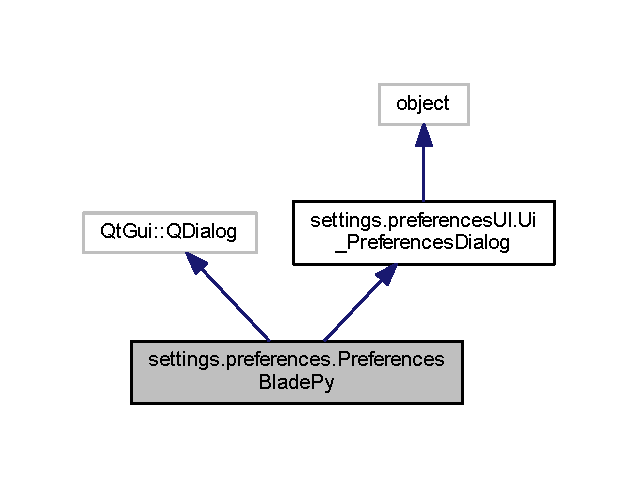
\includegraphics[width=306pt]{classsettings_1_1preferences_1_1_preferences_blade_py__inherit__graph}
\end{center}
\end{figure}
\subsection*{Public Member Functions}
\begin{DoxyCompactItemize}
\item 
def \hyperlink{classsettings_1_1preferences_1_1_preferences_blade_py_af773a0c74e666c299d2334a21966f8c9}{\+\_\+\+\_\+init\+\_\+\+\_\+} (self, parent=None)
\item 
def \hyperlink{classsettings_1_1preferences_1_1_preferences_blade_py_a7e99113696fefa62dfdeb2ba1279350c}{ok\+Action} (self)
\begin{DoxyCompactList}\small\item\em Method for applying user preferences and closing the dialog. \end{DoxyCompactList}\item 
def \hyperlink{classsettings_1_1preferences_1_1_preferences_blade_py_af92de31fcc110a9892dc2914efb6b46f}{cancel\+Action} (self)
\begin{DoxyCompactList}\small\item\em Method simply for closing the dialog. \end{DoxyCompactList}\item 
def \hyperlink{classsettings_1_1preferences_1_1_preferences_blade_py_a8938a7b43ca7c5496a0ae7bf8d6a0c54}{apply\+Action} (self)
\begin{DoxyCompactList}\small\item\em Method for applying user preferences but not closing the dialog. \end{DoxyCompactList}\item 
def \hyperlink{classsettings_1_1preferences_1_1_preferences_blade_py_a9cfbfd7abab4ba14d80c573a0534040b}{save\+Settings} (self, setting)
\begin{DoxyCompactList}\small\item\em Method called by \hyperlink{classsettings_1_1preferences_1_1_preferences_blade_py_a8938a7b43ca7c5496a0ae7bf8d6a0c54}{apply\+Action()} that indeed sets the configurations. \end{DoxyCompactList}\item 
def \hyperlink{classsettings_1_1preferences_1_1_preferences_blade_py_ab74be9049535f502252efb2df560ac8e}{restore\+Standard} (self, setting)
\begin{DoxyCompactList}\small\item\em Method for restoring default configurations. \end{DoxyCompactList}\end{DoxyCompactItemize}
\subsection*{Public Attributes}
\begin{DoxyCompactItemize}
\item 
\hyperlink{classsettings_1_1preferences_1_1_preferences_blade_py_a8904394496c57e265ab1cf0346b025d9}{last\+\_\+settings}
\item 
\hyperlink{classsettings_1_1preferences_1_1_preferences_blade_py_a0a02958126e9787f79af1a0f45fab30c}{user\+\_\+settings}
\item 
\hyperlink{classsettings_1_1preferences_1_1_preferences_blade_py_aec84d483efd9155fc73699fe365ac9c2}{list\+\_\+settings}
\end{DoxyCompactItemize}


\subsection{Detailed Description}
Class with the methods for customizing user preferences. 

\subsection{Constructor \& Destructor Documentation}
\hypertarget{classsettings_1_1preferences_1_1_preferences_blade_py_af773a0c74e666c299d2334a21966f8c9}{}\label{classsettings_1_1preferences_1_1_preferences_blade_py_af773a0c74e666c299d2334a21966f8c9} 
\index{settings\+::preferences\+::\+Preferences\+Blade\+Py@{settings\+::preferences\+::\+Preferences\+Blade\+Py}!\+\_\+\+\_\+init\+\_\+\+\_\+@{\+\_\+\+\_\+init\+\_\+\+\_\+}}
\index{\+\_\+\+\_\+init\+\_\+\+\_\+@{\+\_\+\+\_\+init\+\_\+\+\_\+}!settings\+::preferences\+::\+Preferences\+Blade\+Py@{settings\+::preferences\+::\+Preferences\+Blade\+Py}}
\subsubsection{\texorpdfstring{\+\_\+\+\_\+init\+\_\+\+\_\+()}{\_\_init\_\_()}}
{\footnotesize\ttfamily def settings.\+preferences.\+Preferences\+Blade\+Py.\+\_\+\+\_\+init\+\_\+\+\_\+ (\begin{DoxyParamCaption}\item[{}]{self,  }\item[{}]{parent = {\ttfamily None} }\end{DoxyParamCaption})}



\subsection{Member Function Documentation}
\hypertarget{classsettings_1_1preferences_1_1_preferences_blade_py_a8938a7b43ca7c5496a0ae7bf8d6a0c54}{}\label{classsettings_1_1preferences_1_1_preferences_blade_py_a8938a7b43ca7c5496a0ae7bf8d6a0c54} 
\index{settings\+::preferences\+::\+Preferences\+Blade\+Py@{settings\+::preferences\+::\+Preferences\+Blade\+Py}!apply\+Action@{apply\+Action}}
\index{apply\+Action@{apply\+Action}!settings\+::preferences\+::\+Preferences\+Blade\+Py@{settings\+::preferences\+::\+Preferences\+Blade\+Py}}
\subsubsection{\texorpdfstring{apply\+Action()}{applyAction()}}
{\footnotesize\ttfamily def settings.\+preferences.\+Preferences\+Blade\+Py.\+apply\+Action (\begin{DoxyParamCaption}\item[{}]{self }\end{DoxyParamCaption})}



Method for applying user preferences but not closing the dialog. 

\begin{DoxyReturn}{Returns}
None 
\end{DoxyReturn}
\hypertarget{classsettings_1_1preferences_1_1_preferences_blade_py_af92de31fcc110a9892dc2914efb6b46f}{}\label{classsettings_1_1preferences_1_1_preferences_blade_py_af92de31fcc110a9892dc2914efb6b46f} 
\index{settings\+::preferences\+::\+Preferences\+Blade\+Py@{settings\+::preferences\+::\+Preferences\+Blade\+Py}!cancel\+Action@{cancel\+Action}}
\index{cancel\+Action@{cancel\+Action}!settings\+::preferences\+::\+Preferences\+Blade\+Py@{settings\+::preferences\+::\+Preferences\+Blade\+Py}}
\subsubsection{\texorpdfstring{cancel\+Action()}{cancelAction()}}
{\footnotesize\ttfamily def settings.\+preferences.\+Preferences\+Blade\+Py.\+cancel\+Action (\begin{DoxyParamCaption}\item[{}]{self }\end{DoxyParamCaption})}



Method simply for closing the dialog. 

\begin{DoxyReturn}{Returns}
None 
\end{DoxyReturn}
\hypertarget{classsettings_1_1preferences_1_1_preferences_blade_py_a7e99113696fefa62dfdeb2ba1279350c}{}\label{classsettings_1_1preferences_1_1_preferences_blade_py_a7e99113696fefa62dfdeb2ba1279350c} 
\index{settings\+::preferences\+::\+Preferences\+Blade\+Py@{settings\+::preferences\+::\+Preferences\+Blade\+Py}!ok\+Action@{ok\+Action}}
\index{ok\+Action@{ok\+Action}!settings\+::preferences\+::\+Preferences\+Blade\+Py@{settings\+::preferences\+::\+Preferences\+Blade\+Py}}
\subsubsection{\texorpdfstring{ok\+Action()}{okAction()}}
{\footnotesize\ttfamily def settings.\+preferences.\+Preferences\+Blade\+Py.\+ok\+Action (\begin{DoxyParamCaption}\item[{}]{self }\end{DoxyParamCaption})}



Method for applying user preferences and closing the dialog. 

\begin{DoxyReturn}{Returns}
None 
\end{DoxyReturn}
\hypertarget{classsettings_1_1preferences_1_1_preferences_blade_py_ab74be9049535f502252efb2df560ac8e}{}\label{classsettings_1_1preferences_1_1_preferences_blade_py_ab74be9049535f502252efb2df560ac8e} 
\index{settings\+::preferences\+::\+Preferences\+Blade\+Py@{settings\+::preferences\+::\+Preferences\+Blade\+Py}!restore\+Standard@{restore\+Standard}}
\index{restore\+Standard@{restore\+Standard}!settings\+::preferences\+::\+Preferences\+Blade\+Py@{settings\+::preferences\+::\+Preferences\+Blade\+Py}}
\subsubsection{\texorpdfstring{restore\+Standard()}{restoreStandard()}}
{\footnotesize\ttfamily def settings.\+preferences.\+Preferences\+Blade\+Py.\+restore\+Standard (\begin{DoxyParamCaption}\item[{}]{self,  }\item[{}]{setting }\end{DoxyParamCaption})}



Method for restoring default configurations. 


\begin{DoxyParams}{Parameters}
{\em setting} & \mbox{[}int\mbox{]} always 1 for the moment. It support a number of different settings, but not yet implemented \\
\hline
\end{DoxyParams}
\begin{DoxyReturn}{Returns}
None 
\end{DoxyReturn}
\hypertarget{classsettings_1_1preferences_1_1_preferences_blade_py_a9cfbfd7abab4ba14d80c573a0534040b}{}\label{classsettings_1_1preferences_1_1_preferences_blade_py_a9cfbfd7abab4ba14d80c573a0534040b} 
\index{settings\+::preferences\+::\+Preferences\+Blade\+Py@{settings\+::preferences\+::\+Preferences\+Blade\+Py}!save\+Settings@{save\+Settings}}
\index{save\+Settings@{save\+Settings}!settings\+::preferences\+::\+Preferences\+Blade\+Py@{settings\+::preferences\+::\+Preferences\+Blade\+Py}}
\subsubsection{\texorpdfstring{save\+Settings()}{saveSettings()}}
{\footnotesize\ttfamily def settings.\+preferences.\+Preferences\+Blade\+Py.\+save\+Settings (\begin{DoxyParamCaption}\item[{}]{self,  }\item[{}]{setting }\end{DoxyParamCaption})}



Method called by \hyperlink{classsettings_1_1preferences_1_1_preferences_blade_py_a8938a7b43ca7c5496a0ae7bf8d6a0c54}{apply\+Action()} that indeed sets the configurations. 


\begin{DoxyParams}{Parameters}
{\em setting} & \mbox{[}int\mbox{]} always 1 for the moment. It support a number of different settings, but not yet implemented \\
\hline
\end{DoxyParams}
\begin{DoxyReturn}{Returns}
None 
\end{DoxyReturn}


\subsection{Member Data Documentation}
\hypertarget{classsettings_1_1preferences_1_1_preferences_blade_py_a8904394496c57e265ab1cf0346b025d9}{}\label{classsettings_1_1preferences_1_1_preferences_blade_py_a8904394496c57e265ab1cf0346b025d9} 
\index{settings\+::preferences\+::\+Preferences\+Blade\+Py@{settings\+::preferences\+::\+Preferences\+Blade\+Py}!last\+\_\+settings@{last\+\_\+settings}}
\index{last\+\_\+settings@{last\+\_\+settings}!settings\+::preferences\+::\+Preferences\+Blade\+Py@{settings\+::preferences\+::\+Preferences\+Blade\+Py}}
\subsubsection{\texorpdfstring{last\+\_\+settings}{last\_settings}}
{\footnotesize\ttfamily settings.\+preferences.\+Preferences\+Blade\+Py.\+last\+\_\+settings}

\hypertarget{classsettings_1_1preferences_1_1_preferences_blade_py_aec84d483efd9155fc73699fe365ac9c2}{}\label{classsettings_1_1preferences_1_1_preferences_blade_py_aec84d483efd9155fc73699fe365ac9c2} 
\index{settings\+::preferences\+::\+Preferences\+Blade\+Py@{settings\+::preferences\+::\+Preferences\+Blade\+Py}!list\+\_\+settings@{list\+\_\+settings}}
\index{list\+\_\+settings@{list\+\_\+settings}!settings\+::preferences\+::\+Preferences\+Blade\+Py@{settings\+::preferences\+::\+Preferences\+Blade\+Py}}
\subsubsection{\texorpdfstring{list\+\_\+settings}{list\_settings}}
{\footnotesize\ttfamily settings.\+preferences.\+Preferences\+Blade\+Py.\+list\+\_\+settings}

\hypertarget{classsettings_1_1preferences_1_1_preferences_blade_py_a0a02958126e9787f79af1a0f45fab30c}{}\label{classsettings_1_1preferences_1_1_preferences_blade_py_a0a02958126e9787f79af1a0f45fab30c} 
\index{settings\+::preferences\+::\+Preferences\+Blade\+Py@{settings\+::preferences\+::\+Preferences\+Blade\+Py}!user\+\_\+settings@{user\+\_\+settings}}
\index{user\+\_\+settings@{user\+\_\+settings}!settings\+::preferences\+::\+Preferences\+Blade\+Py@{settings\+::preferences\+::\+Preferences\+Blade\+Py}}
\subsubsection{\texorpdfstring{user\+\_\+settings}{user\_settings}}
{\footnotesize\ttfamily settings.\+preferences.\+Preferences\+Blade\+Py.\+user\+\_\+settings}



The documentation for this class was generated from the following file\+:\begin{DoxyCompactItemize}
\item 
\hyperlink{preferences_8py}{preferences.\+py}\end{DoxyCompactItemize}

\hypertarget{classocc__modules_1_1shape__properties_1_1_shape_manager}{}\section{occ\+\_\+modules.\+shape\+\_\+properties.\+Shape\+Manager Class Reference}
\label{classocc__modules_1_1shape__properties_1_1_shape_manager}\index{occ\+\_\+modules.\+shape\+\_\+properties.\+Shape\+Manager@{occ\+\_\+modules.\+shape\+\_\+properties.\+Shape\+Manager}}


This class is a group of methods related to shape properties control.  




Inheritance diagram for occ\+\_\+modules.\+shape\+\_\+properties.\+Shape\+Manager\+:\nopagebreak
\begin{figure}[H]
\begin{center}
\leavevmode
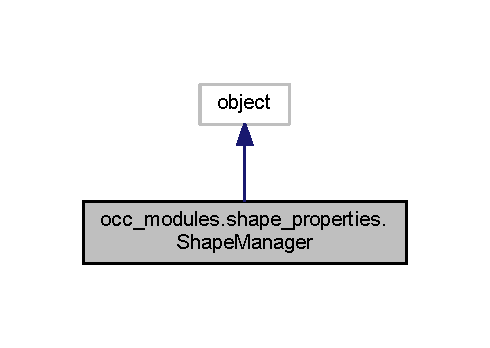
\includegraphics[width=235pt]{classocc__modules_1_1shape__properties_1_1_shape_manager__inherit__graph}
\end{center}
\end{figure}
\subsection*{Public Member Functions}
\begin{DoxyCompactItemize}
\item 
def \hyperlink{classocc__modules_1_1shape__properties_1_1_shape_manager_aeafd1ea7cbe63a409e51e546db403bfd}{\+\_\+\+\_\+init\+\_\+\+\_\+} (self, Output\+Viewer\+Widget)
\item 
def \hyperlink{classocc__modules_1_1shape__properties_1_1_shape_manager_a8833b4dba535cb76318777c031cf08b5}{load\+Shape} (self, shape\+\_\+list)
\begin{DoxyCompactList}\small\item\em Method for loading one or more shapes and displaying to Output Viewer. \end{DoxyCompactList}\item 
def \hyperlink{classocc__modules_1_1shape__properties_1_1_shape_manager_abe8c1dbcfe98b9f86a0560dd1e8b853a}{set\+Quality} (self)
\begin{DoxyCompactList}\small\item\em Sets quality to the current working A\+IS Shape. \end{DoxyCompactList}\item 
def \hyperlink{classocc__modules_1_1shape__properties_1_1_shape_manager_a8d7fdd0bde28afe34d3793c8bcf060fa}{set\+Transparency} (self)
\begin{DoxyCompactList}\small\item\em Sets transparency to the current working A\+IS Shape. \end{DoxyCompactList}\item 
def \hyperlink{classocc__modules_1_1shape__properties_1_1_shape_manager_ac659823f3085963daf751a6a94b366a7}{set\+Color} (self)
\begin{DoxyCompactList}\small\item\em Sets color to the current working A\+IS Shape. \end{DoxyCompactList}\item 
def \hyperlink{classocc__modules_1_1shape__properties_1_1_shape_manager_a1cab1ea26a1cd0091d88106b6b4715bb}{set\+Translation} (self)
\begin{DoxyCompactList}\small\item\em Creates an axis in x, y or z depending on user preference. \end{DoxyCompactList}\item 
def \hyperlink{classocc__modules_1_1shape__properties_1_1_shape_manager_ad4293087adb512ea61fe0c3429c0e08c}{hide\+Shape} (self)
\begin{DoxyCompactList}\small\item\em Method for hiding selected shape. \end{DoxyCompactList}\item 
def \hyperlink{classocc__modules_1_1shape__properties_1_1_shape_manager_aba26c11e7e7ec6c2c6709a27cbeaaf69}{display\+Shape} (self)
\begin{DoxyCompactList}\small\item\em Method for displaying selected shape. \end{DoxyCompactList}\end{DoxyCompactItemize}
\subsection*{Public Attributes}
\begin{DoxyCompactItemize}
\item 
\hyperlink{classocc__modules_1_1shape__properties_1_1_shape_manager_ad60197d66a3c059f30f32c2ab1a12841}{op\+\_\+viewer}
\begin{DoxyCompactList}\small\item\em Object reference to main object. \end{DoxyCompactList}\end{DoxyCompactItemize}


\subsection{Detailed Description}
This class is a group of methods related to shape properties control. 

All these methods are a linked to \hyperlink{class_core_1_1_blade_py_core}{Core.\+Blade\+Py\+Core} by composition. Contains methods that manages the Shape appearance such transparency, quality, color. It also has a method capable of transforming the shape by displacing or rotating it. 

\subsection{Constructor \& Destructor Documentation}
\hypertarget{classocc__modules_1_1shape__properties_1_1_shape_manager_aeafd1ea7cbe63a409e51e546db403bfd}{}\label{classocc__modules_1_1shape__properties_1_1_shape_manager_aeafd1ea7cbe63a409e51e546db403bfd} 
\index{occ\+\_\+modules\+::shape\+\_\+properties\+::\+Shape\+Manager@{occ\+\_\+modules\+::shape\+\_\+properties\+::\+Shape\+Manager}!\+\_\+\+\_\+init\+\_\+\+\_\+@{\+\_\+\+\_\+init\+\_\+\+\_\+}}
\index{\+\_\+\+\_\+init\+\_\+\+\_\+@{\+\_\+\+\_\+init\+\_\+\+\_\+}!occ\+\_\+modules\+::shape\+\_\+properties\+::\+Shape\+Manager@{occ\+\_\+modules\+::shape\+\_\+properties\+::\+Shape\+Manager}}
\subsubsection{\texorpdfstring{\+\_\+\+\_\+init\+\_\+\+\_\+()}{\_\_init\_\_()}}
{\footnotesize\ttfamily def occ\+\_\+modules.\+shape\+\_\+properties.\+Shape\+Manager.\+\_\+\+\_\+init\+\_\+\+\_\+ (\begin{DoxyParamCaption}\item[{}]{self,  }\item[{}]{Output\+Viewer\+Widget }\end{DoxyParamCaption})}



\subsection{Member Function Documentation}
\hypertarget{classocc__modules_1_1shape__properties_1_1_shape_manager_aba26c11e7e7ec6c2c6709a27cbeaaf69}{}\label{classocc__modules_1_1shape__properties_1_1_shape_manager_aba26c11e7e7ec6c2c6709a27cbeaaf69} 
\index{occ\+\_\+modules\+::shape\+\_\+properties\+::\+Shape\+Manager@{occ\+\_\+modules\+::shape\+\_\+properties\+::\+Shape\+Manager}!display\+Shape@{display\+Shape}}
\index{display\+Shape@{display\+Shape}!occ\+\_\+modules\+::shape\+\_\+properties\+::\+Shape\+Manager@{occ\+\_\+modules\+::shape\+\_\+properties\+::\+Shape\+Manager}}
\subsubsection{\texorpdfstring{display\+Shape()}{displayShape()}}
{\footnotesize\ttfamily def occ\+\_\+modules.\+shape\+\_\+properties.\+Shape\+Manager.\+display\+Shape (\begin{DoxyParamCaption}\item[{}]{self }\end{DoxyParamCaption})}



Method for displaying selected shape. 

\begin{DoxyReturn}{Returns}
None 
\end{DoxyReturn}
\hypertarget{classocc__modules_1_1shape__properties_1_1_shape_manager_ad4293087adb512ea61fe0c3429c0e08c}{}\label{classocc__modules_1_1shape__properties_1_1_shape_manager_ad4293087adb512ea61fe0c3429c0e08c} 
\index{occ\+\_\+modules\+::shape\+\_\+properties\+::\+Shape\+Manager@{occ\+\_\+modules\+::shape\+\_\+properties\+::\+Shape\+Manager}!hide\+Shape@{hide\+Shape}}
\index{hide\+Shape@{hide\+Shape}!occ\+\_\+modules\+::shape\+\_\+properties\+::\+Shape\+Manager@{occ\+\_\+modules\+::shape\+\_\+properties\+::\+Shape\+Manager}}
\subsubsection{\texorpdfstring{hide\+Shape()}{hideShape()}}
{\footnotesize\ttfamily def occ\+\_\+modules.\+shape\+\_\+properties.\+Shape\+Manager.\+hide\+Shape (\begin{DoxyParamCaption}\item[{}]{self }\end{DoxyParamCaption})}



Method for hiding selected shape. 

\begin{DoxyReturn}{Returns}
None 
\end{DoxyReturn}
\hypertarget{classocc__modules_1_1shape__properties_1_1_shape_manager_a8833b4dba535cb76318777c031cf08b5}{}\label{classocc__modules_1_1shape__properties_1_1_shape_manager_a8833b4dba535cb76318777c031cf08b5} 
\index{occ\+\_\+modules\+::shape\+\_\+properties\+::\+Shape\+Manager@{occ\+\_\+modules\+::shape\+\_\+properties\+::\+Shape\+Manager}!load\+Shape@{load\+Shape}}
\index{load\+Shape@{load\+Shape}!occ\+\_\+modules\+::shape\+\_\+properties\+::\+Shape\+Manager@{occ\+\_\+modules\+::shape\+\_\+properties\+::\+Shape\+Manager}}
\subsubsection{\texorpdfstring{load\+Shape()}{loadShape()}}
{\footnotesize\ttfamily def occ\+\_\+modules.\+shape\+\_\+properties.\+Shape\+Manager.\+load\+Shape (\begin{DoxyParamCaption}\item[{}]{self,  }\item[{}]{shape\+\_\+list }\end{DoxyParamCaption})}



Method for loading one or more shapes and displaying to Output Viewer. 

This method uses libraries of iges caf control for fetching sub-\/shape names within .igs files. This method is used when adding a case in the main routine.


\begin{DoxyParams}{Parameters}
{\em shape\+\_\+list} & \mbox{[}list\mbox{]} First index contains the path of shape, second index contains a list of display exceptions, e.\+g\+: \mbox{[}\mbox{[}igs\+\_\+2d\+\_\+shape\+\_\+path, \mbox{[}\char`\"{}\+H\+U\+B\char`\"{}, \char`\"{}\+S\+H\+R\+O\+U\+D\char`\"{}\mbox{]}, \mbox{[}igs\+\_\+3d\+\_\+shape\+\_\+path, \mbox{[}\char`\"{}\+S\+T\+R\+E\+A\+M\char`\"{}\mbox{]}\mbox{]} \\
\hline
\end{DoxyParams}
\begin{DoxyReturn}{Returns}
First return contains list of ais\+\_\+shapes handles and second return contains a list of sub-\/shape names in strings 
\end{DoxyReturn}
\hypertarget{classocc__modules_1_1shape__properties_1_1_shape_manager_ac659823f3085963daf751a6a94b366a7}{}\label{classocc__modules_1_1shape__properties_1_1_shape_manager_ac659823f3085963daf751a6a94b366a7} 
\index{occ\+\_\+modules\+::shape\+\_\+properties\+::\+Shape\+Manager@{occ\+\_\+modules\+::shape\+\_\+properties\+::\+Shape\+Manager}!set\+Color@{set\+Color}}
\index{set\+Color@{set\+Color}!occ\+\_\+modules\+::shape\+\_\+properties\+::\+Shape\+Manager@{occ\+\_\+modules\+::shape\+\_\+properties\+::\+Shape\+Manager}}
\subsubsection{\texorpdfstring{set\+Color()}{setColor()}}
{\footnotesize\ttfamily def occ\+\_\+modules.\+shape\+\_\+properties.\+Shape\+Manager.\+set\+Color (\begin{DoxyParamCaption}\item[{}]{self }\end{DoxyParamCaption})}



Sets color to the current working A\+IS Shape. 

\begin{DoxyReturn}{Returns}
None 
\end{DoxyReturn}
\hypertarget{classocc__modules_1_1shape__properties_1_1_shape_manager_abe8c1dbcfe98b9f86a0560dd1e8b853a}{}\label{classocc__modules_1_1shape__properties_1_1_shape_manager_abe8c1dbcfe98b9f86a0560dd1e8b853a} 
\index{occ\+\_\+modules\+::shape\+\_\+properties\+::\+Shape\+Manager@{occ\+\_\+modules\+::shape\+\_\+properties\+::\+Shape\+Manager}!set\+Quality@{set\+Quality}}
\index{set\+Quality@{set\+Quality}!occ\+\_\+modules\+::shape\+\_\+properties\+::\+Shape\+Manager@{occ\+\_\+modules\+::shape\+\_\+properties\+::\+Shape\+Manager}}
\subsubsection{\texorpdfstring{set\+Quality()}{setQuality()}}
{\footnotesize\ttfamily def occ\+\_\+modules.\+shape\+\_\+properties.\+Shape\+Manager.\+set\+Quality (\begin{DoxyParamCaption}\item[{}]{self }\end{DoxyParamCaption})}



Sets quality to the current working A\+IS Shape. 

\begin{DoxyReturn}{Returns}
None 
\end{DoxyReturn}
\hypertarget{classocc__modules_1_1shape__properties_1_1_shape_manager_a1cab1ea26a1cd0091d88106b6b4715bb}{}\label{classocc__modules_1_1shape__properties_1_1_shape_manager_a1cab1ea26a1cd0091d88106b6b4715bb} 
\index{occ\+\_\+modules\+::shape\+\_\+properties\+::\+Shape\+Manager@{occ\+\_\+modules\+::shape\+\_\+properties\+::\+Shape\+Manager}!set\+Translation@{set\+Translation}}
\index{set\+Translation@{set\+Translation}!occ\+\_\+modules\+::shape\+\_\+properties\+::\+Shape\+Manager@{occ\+\_\+modules\+::shape\+\_\+properties\+::\+Shape\+Manager}}
\subsubsection{\texorpdfstring{set\+Translation()}{setTranslation()}}
{\footnotesize\ttfamily def occ\+\_\+modules.\+shape\+\_\+properties.\+Shape\+Manager.\+set\+Translation (\begin{DoxyParamCaption}\item[{}]{self }\end{DoxyParamCaption})}



Creates an axis in x, y or z depending on user preference. 

gp\+\_\+\+Ax1 describes an axis in 3D space. An axis is defined by a point (gp\+\_\+\+Pnt) and a direction (gp\+\_\+\+Dir) reference

\begin{DoxyReturn}{Returns}
None 
\end{DoxyReturn}
\hypertarget{classocc__modules_1_1shape__properties_1_1_shape_manager_a8d7fdd0bde28afe34d3793c8bcf060fa}{}\label{classocc__modules_1_1shape__properties_1_1_shape_manager_a8d7fdd0bde28afe34d3793c8bcf060fa} 
\index{occ\+\_\+modules\+::shape\+\_\+properties\+::\+Shape\+Manager@{occ\+\_\+modules\+::shape\+\_\+properties\+::\+Shape\+Manager}!set\+Transparency@{set\+Transparency}}
\index{set\+Transparency@{set\+Transparency}!occ\+\_\+modules\+::shape\+\_\+properties\+::\+Shape\+Manager@{occ\+\_\+modules\+::shape\+\_\+properties\+::\+Shape\+Manager}}
\subsubsection{\texorpdfstring{set\+Transparency()}{setTransparency()}}
{\footnotesize\ttfamily def occ\+\_\+modules.\+shape\+\_\+properties.\+Shape\+Manager.\+set\+Transparency (\begin{DoxyParamCaption}\item[{}]{self }\end{DoxyParamCaption})}



Sets transparency to the current working A\+IS Shape. 

\begin{DoxyReturn}{Returns}
None 
\end{DoxyReturn}


\subsection{Member Data Documentation}
\hypertarget{classocc__modules_1_1shape__properties_1_1_shape_manager_ad60197d66a3c059f30f32c2ab1a12841}{}\label{classocc__modules_1_1shape__properties_1_1_shape_manager_ad60197d66a3c059f30f32c2ab1a12841} 
\index{occ\+\_\+modules\+::shape\+\_\+properties\+::\+Shape\+Manager@{occ\+\_\+modules\+::shape\+\_\+properties\+::\+Shape\+Manager}!op\+\_\+viewer@{op\+\_\+viewer}}
\index{op\+\_\+viewer@{op\+\_\+viewer}!occ\+\_\+modules\+::shape\+\_\+properties\+::\+Shape\+Manager@{occ\+\_\+modules\+::shape\+\_\+properties\+::\+Shape\+Manager}}
\subsubsection{\texorpdfstring{op\+\_\+viewer}{op\_viewer}}
{\footnotesize\ttfamily occ\+\_\+modules.\+shape\+\_\+properties.\+Shape\+Manager.\+op\+\_\+viewer}



Object reference to main object. 



The documentation for this class was generated from the following file\+:\begin{DoxyCompactItemize}
\item 
\hyperlink{shape__properties_8py}{shape\+\_\+properties.\+py}\end{DoxyCompactItemize}

\hypertarget{classtecplot__modules_1_1tecplot__reader_1_1_tec_plot_core}{}\section{tecplot\+\_\+modules.\+tecplot\+\_\+reader.\+Tec\+Plot\+Core Class Reference}
\label{classtecplot__modules_1_1tecplot__reader_1_1_tec_plot_core}\index{tecplot\+\_\+modules.\+tecplot\+\_\+reader.\+Tec\+Plot\+Core@{tecplot\+\_\+modules.\+tecplot\+\_\+reader.\+Tec\+Plot\+Core}}


Class for reading tecplot outputs.  




Inheritance diagram for tecplot\+\_\+modules.\+tecplot\+\_\+reader.\+Tec\+Plot\+Core\+:\nopagebreak
\begin{figure}[H]
\begin{center}
\leavevmode
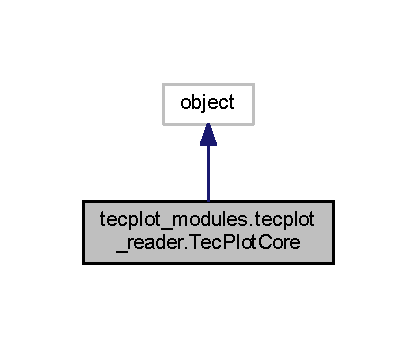
\includegraphics[width=200pt]{classtecplot__modules_1_1tecplot__reader_1_1_tec_plot_core__inherit__graph}
\end{center}
\end{figure}
\subsection*{Public Member Functions}
\begin{DoxyCompactItemize}
\item 
def \hyperlink{classtecplot__modules_1_1tecplot__reader_1_1_tec_plot_core_a15954180c0b4a9677efd980873a91773}{\+\_\+\+\_\+init\+\_\+\+\_\+} (self)
\item 
def \hyperlink{classtecplot__modules_1_1tecplot__reader_1_1_tec_plot_core_a9cf438934b57cd1d0bef90bcc00f27ac}{tecplot\+Reader} (self, read\+\_\+csv)
\begin{DoxyCompactList}\small\item\em Function to dig into a csv file and to record it to instance variables lists. \end{DoxyCompactList}\end{DoxyCompactItemize}
\subsection*{Public Attributes}
\begin{DoxyCompactItemize}
\item 
\hyperlink{classtecplot__modules_1_1tecplot__reader_1_1_tec_plot_core_a2ccc38e7f7503e06d5c5fad58a071f80}{hub\+\_\+coordinates}
\item 
\hyperlink{classtecplot__modules_1_1tecplot__reader_1_1_tec_plot_core_a583d4851d722f76e18ec7841357b4ea7}{shroud\+\_\+coordinates}
\item 
\hyperlink{classtecplot__modules_1_1tecplot__reader_1_1_tec_plot_core_ab6edfe4cfa33db98eb1414228f78a303}{trailing\+\_\+coordinates}
\item 
\hyperlink{classtecplot__modules_1_1tecplot__reader_1_1_tec_plot_core_af991756a166df02da0a122d8d7c5c372}{leading\+\_\+coordinates}
\item 
\hyperlink{classtecplot__modules_1_1tecplot__reader_1_1_tec_plot_core_a4c8e60241684e96d45eabfb99e6955fd}{stream\+\_\+coordinates}
\item 
\hyperlink{classtecplot__modules_1_1tecplot__reader_1_1_tec_plot_core_abd9898f018cbb1686522d50721f851a7}{bladeprofile\+\_\+coordinates}
\item 
\hyperlink{classtecplot__modules_1_1tecplot__reader_1_1_tec_plot_core_a33fc4c19a7badee5e2a88f3be97f8efb}{meanline\+\_\+coordinates}
\item 
\hyperlink{classtecplot__modules_1_1tecplot__reader_1_1_tec_plot_core_a894f4ab5042e885fa8349c50c37059ac}{thickness\+\_\+coordinates}
\end{DoxyCompactItemize}


\subsection{Detailed Description}
Class for reading tecplot outputs. 

A object of this class will be in a composition association with a object of a \hyperlink{classtecplot__modules_1_1tecplot__display_1_1_tec_plot_window}{tecplot\+\_\+display.\+Tec\+Plot\+Window} class. 

\subsection{Constructor \& Destructor Documentation}
\hypertarget{classtecplot__modules_1_1tecplot__reader_1_1_tec_plot_core_a15954180c0b4a9677efd980873a91773}{}\label{classtecplot__modules_1_1tecplot__reader_1_1_tec_plot_core_a15954180c0b4a9677efd980873a91773} 
\index{tecplot\+\_\+modules\+::tecplot\+\_\+reader\+::\+Tec\+Plot\+Core@{tecplot\+\_\+modules\+::tecplot\+\_\+reader\+::\+Tec\+Plot\+Core}!\+\_\+\+\_\+init\+\_\+\+\_\+@{\+\_\+\+\_\+init\+\_\+\+\_\+}}
\index{\+\_\+\+\_\+init\+\_\+\+\_\+@{\+\_\+\+\_\+init\+\_\+\+\_\+}!tecplot\+\_\+modules\+::tecplot\+\_\+reader\+::\+Tec\+Plot\+Core@{tecplot\+\_\+modules\+::tecplot\+\_\+reader\+::\+Tec\+Plot\+Core}}
\subsubsection{\texorpdfstring{\+\_\+\+\_\+init\+\_\+\+\_\+()}{\_\_init\_\_()}}
{\footnotesize\ttfamily def tecplot\+\_\+modules.\+tecplot\+\_\+reader.\+Tec\+Plot\+Core.\+\_\+\+\_\+init\+\_\+\+\_\+ (\begin{DoxyParamCaption}\item[{}]{self }\end{DoxyParamCaption})}



\subsection{Member Function Documentation}
\hypertarget{classtecplot__modules_1_1tecplot__reader_1_1_tec_plot_core_a9cf438934b57cd1d0bef90bcc00f27ac}{}\label{classtecplot__modules_1_1tecplot__reader_1_1_tec_plot_core_a9cf438934b57cd1d0bef90bcc00f27ac} 
\index{tecplot\+\_\+modules\+::tecplot\+\_\+reader\+::\+Tec\+Plot\+Core@{tecplot\+\_\+modules\+::tecplot\+\_\+reader\+::\+Tec\+Plot\+Core}!tecplot\+Reader@{tecplot\+Reader}}
\index{tecplot\+Reader@{tecplot\+Reader}!tecplot\+\_\+modules\+::tecplot\+\_\+reader\+::\+Tec\+Plot\+Core@{tecplot\+\_\+modules\+::tecplot\+\_\+reader\+::\+Tec\+Plot\+Core}}
\subsubsection{\texorpdfstring{tecplot\+Reader()}{tecplotReader()}}
{\footnotesize\ttfamily def tecplot\+\_\+modules.\+tecplot\+\_\+reader.\+Tec\+Plot\+Core.\+tecplot\+Reader (\begin{DoxyParamCaption}\item[{}]{self,  }\item[{}]{read\+\_\+csv }\end{DoxyParamCaption})}



Function to dig into a csv file and to record it to instance variables lists. 


\begin{DoxyParams}{Parameters}
{\em read\+\_\+csv} & \mbox{[}csv\+\_\+file\mbox{]} The file where tecplot data is \\
\hline
\end{DoxyParams}
\begin{DoxyReturn}{Returns}
None 
\end{DoxyReturn}


\subsection{Member Data Documentation}
\hypertarget{classtecplot__modules_1_1tecplot__reader_1_1_tec_plot_core_abd9898f018cbb1686522d50721f851a7}{}\label{classtecplot__modules_1_1tecplot__reader_1_1_tec_plot_core_abd9898f018cbb1686522d50721f851a7} 
\index{tecplot\+\_\+modules\+::tecplot\+\_\+reader\+::\+Tec\+Plot\+Core@{tecplot\+\_\+modules\+::tecplot\+\_\+reader\+::\+Tec\+Plot\+Core}!bladeprofile\+\_\+coordinates@{bladeprofile\+\_\+coordinates}}
\index{bladeprofile\+\_\+coordinates@{bladeprofile\+\_\+coordinates}!tecplot\+\_\+modules\+::tecplot\+\_\+reader\+::\+Tec\+Plot\+Core@{tecplot\+\_\+modules\+::tecplot\+\_\+reader\+::\+Tec\+Plot\+Core}}
\subsubsection{\texorpdfstring{bladeprofile\+\_\+coordinates}{bladeprofile\_coordinates}}
{\footnotesize\ttfamily tecplot\+\_\+modules.\+tecplot\+\_\+reader.\+Tec\+Plot\+Core.\+bladeprofile\+\_\+coordinates}

\hypertarget{classtecplot__modules_1_1tecplot__reader_1_1_tec_plot_core_a2ccc38e7f7503e06d5c5fad58a071f80}{}\label{classtecplot__modules_1_1tecplot__reader_1_1_tec_plot_core_a2ccc38e7f7503e06d5c5fad58a071f80} 
\index{tecplot\+\_\+modules\+::tecplot\+\_\+reader\+::\+Tec\+Plot\+Core@{tecplot\+\_\+modules\+::tecplot\+\_\+reader\+::\+Tec\+Plot\+Core}!hub\+\_\+coordinates@{hub\+\_\+coordinates}}
\index{hub\+\_\+coordinates@{hub\+\_\+coordinates}!tecplot\+\_\+modules\+::tecplot\+\_\+reader\+::\+Tec\+Plot\+Core@{tecplot\+\_\+modules\+::tecplot\+\_\+reader\+::\+Tec\+Plot\+Core}}
\subsubsection{\texorpdfstring{hub\+\_\+coordinates}{hub\_coordinates}}
{\footnotesize\ttfamily tecplot\+\_\+modules.\+tecplot\+\_\+reader.\+Tec\+Plot\+Core.\+hub\+\_\+coordinates}

\hypertarget{classtecplot__modules_1_1tecplot__reader_1_1_tec_plot_core_af991756a166df02da0a122d8d7c5c372}{}\label{classtecplot__modules_1_1tecplot__reader_1_1_tec_plot_core_af991756a166df02da0a122d8d7c5c372} 
\index{tecplot\+\_\+modules\+::tecplot\+\_\+reader\+::\+Tec\+Plot\+Core@{tecplot\+\_\+modules\+::tecplot\+\_\+reader\+::\+Tec\+Plot\+Core}!leading\+\_\+coordinates@{leading\+\_\+coordinates}}
\index{leading\+\_\+coordinates@{leading\+\_\+coordinates}!tecplot\+\_\+modules\+::tecplot\+\_\+reader\+::\+Tec\+Plot\+Core@{tecplot\+\_\+modules\+::tecplot\+\_\+reader\+::\+Tec\+Plot\+Core}}
\subsubsection{\texorpdfstring{leading\+\_\+coordinates}{leading\_coordinates}}
{\footnotesize\ttfamily tecplot\+\_\+modules.\+tecplot\+\_\+reader.\+Tec\+Plot\+Core.\+leading\+\_\+coordinates}

\hypertarget{classtecplot__modules_1_1tecplot__reader_1_1_tec_plot_core_a33fc4c19a7badee5e2a88f3be97f8efb}{}\label{classtecplot__modules_1_1tecplot__reader_1_1_tec_plot_core_a33fc4c19a7badee5e2a88f3be97f8efb} 
\index{tecplot\+\_\+modules\+::tecplot\+\_\+reader\+::\+Tec\+Plot\+Core@{tecplot\+\_\+modules\+::tecplot\+\_\+reader\+::\+Tec\+Plot\+Core}!meanline\+\_\+coordinates@{meanline\+\_\+coordinates}}
\index{meanline\+\_\+coordinates@{meanline\+\_\+coordinates}!tecplot\+\_\+modules\+::tecplot\+\_\+reader\+::\+Tec\+Plot\+Core@{tecplot\+\_\+modules\+::tecplot\+\_\+reader\+::\+Tec\+Plot\+Core}}
\subsubsection{\texorpdfstring{meanline\+\_\+coordinates}{meanline\_coordinates}}
{\footnotesize\ttfamily tecplot\+\_\+modules.\+tecplot\+\_\+reader.\+Tec\+Plot\+Core.\+meanline\+\_\+coordinates}

\hypertarget{classtecplot__modules_1_1tecplot__reader_1_1_tec_plot_core_a583d4851d722f76e18ec7841357b4ea7}{}\label{classtecplot__modules_1_1tecplot__reader_1_1_tec_plot_core_a583d4851d722f76e18ec7841357b4ea7} 
\index{tecplot\+\_\+modules\+::tecplot\+\_\+reader\+::\+Tec\+Plot\+Core@{tecplot\+\_\+modules\+::tecplot\+\_\+reader\+::\+Tec\+Plot\+Core}!shroud\+\_\+coordinates@{shroud\+\_\+coordinates}}
\index{shroud\+\_\+coordinates@{shroud\+\_\+coordinates}!tecplot\+\_\+modules\+::tecplot\+\_\+reader\+::\+Tec\+Plot\+Core@{tecplot\+\_\+modules\+::tecplot\+\_\+reader\+::\+Tec\+Plot\+Core}}
\subsubsection{\texorpdfstring{shroud\+\_\+coordinates}{shroud\_coordinates}}
{\footnotesize\ttfamily tecplot\+\_\+modules.\+tecplot\+\_\+reader.\+Tec\+Plot\+Core.\+shroud\+\_\+coordinates}

\hypertarget{classtecplot__modules_1_1tecplot__reader_1_1_tec_plot_core_a4c8e60241684e96d45eabfb99e6955fd}{}\label{classtecplot__modules_1_1tecplot__reader_1_1_tec_plot_core_a4c8e60241684e96d45eabfb99e6955fd} 
\index{tecplot\+\_\+modules\+::tecplot\+\_\+reader\+::\+Tec\+Plot\+Core@{tecplot\+\_\+modules\+::tecplot\+\_\+reader\+::\+Tec\+Plot\+Core}!stream\+\_\+coordinates@{stream\+\_\+coordinates}}
\index{stream\+\_\+coordinates@{stream\+\_\+coordinates}!tecplot\+\_\+modules\+::tecplot\+\_\+reader\+::\+Tec\+Plot\+Core@{tecplot\+\_\+modules\+::tecplot\+\_\+reader\+::\+Tec\+Plot\+Core}}
\subsubsection{\texorpdfstring{stream\+\_\+coordinates}{stream\_coordinates}}
{\footnotesize\ttfamily tecplot\+\_\+modules.\+tecplot\+\_\+reader.\+Tec\+Plot\+Core.\+stream\+\_\+coordinates}

\hypertarget{classtecplot__modules_1_1tecplot__reader_1_1_tec_plot_core_a894f4ab5042e885fa8349c50c37059ac}{}\label{classtecplot__modules_1_1tecplot__reader_1_1_tec_plot_core_a894f4ab5042e885fa8349c50c37059ac} 
\index{tecplot\+\_\+modules\+::tecplot\+\_\+reader\+::\+Tec\+Plot\+Core@{tecplot\+\_\+modules\+::tecplot\+\_\+reader\+::\+Tec\+Plot\+Core}!thickness\+\_\+coordinates@{thickness\+\_\+coordinates}}
\index{thickness\+\_\+coordinates@{thickness\+\_\+coordinates}!tecplot\+\_\+modules\+::tecplot\+\_\+reader\+::\+Tec\+Plot\+Core@{tecplot\+\_\+modules\+::tecplot\+\_\+reader\+::\+Tec\+Plot\+Core}}
\subsubsection{\texorpdfstring{thickness\+\_\+coordinates}{thickness\_coordinates}}
{\footnotesize\ttfamily tecplot\+\_\+modules.\+tecplot\+\_\+reader.\+Tec\+Plot\+Core.\+thickness\+\_\+coordinates}

\hypertarget{classtecplot__modules_1_1tecplot__reader_1_1_tec_plot_core_ab6edfe4cfa33db98eb1414228f78a303}{}\label{classtecplot__modules_1_1tecplot__reader_1_1_tec_plot_core_ab6edfe4cfa33db98eb1414228f78a303} 
\index{tecplot\+\_\+modules\+::tecplot\+\_\+reader\+::\+Tec\+Plot\+Core@{tecplot\+\_\+modules\+::tecplot\+\_\+reader\+::\+Tec\+Plot\+Core}!trailing\+\_\+coordinates@{trailing\+\_\+coordinates}}
\index{trailing\+\_\+coordinates@{trailing\+\_\+coordinates}!tecplot\+\_\+modules\+::tecplot\+\_\+reader\+::\+Tec\+Plot\+Core@{tecplot\+\_\+modules\+::tecplot\+\_\+reader\+::\+Tec\+Plot\+Core}}
\subsubsection{\texorpdfstring{trailing\+\_\+coordinates}{trailing\_coordinates}}
{\footnotesize\ttfamily tecplot\+\_\+modules.\+tecplot\+\_\+reader.\+Tec\+Plot\+Core.\+trailing\+\_\+coordinates}



The documentation for this class was generated from the following file\+:\begin{DoxyCompactItemize}
\item 
\hyperlink{tecplot__reader_8py}{tecplot\+\_\+reader.\+py}\end{DoxyCompactItemize}

\hypertarget{classtecplot__modules_1_1tecplot__display_1_1_tec_plot_window}{}\section{tecplot\+\_\+modules.\+tecplot\+\_\+display.\+Tec\+Plot\+Window Class Reference}
\label{classtecplot__modules_1_1tecplot__display_1_1_tec_plot_window}\index{tecplot\+\_\+modules.\+tecplot\+\_\+display.\+Tec\+Plot\+Window@{tecplot\+\_\+modules.\+tecplot\+\_\+display.\+Tec\+Plot\+Window}}


Class for creating a G\+UI for the Blade\+Py Tecplot\+Viewer Widget.  




Inheritance diagram for tecplot\+\_\+modules.\+tecplot\+\_\+display.\+Tec\+Plot\+Window\+:\nopagebreak
\begin{figure}[H]
\begin{center}
\leavevmode
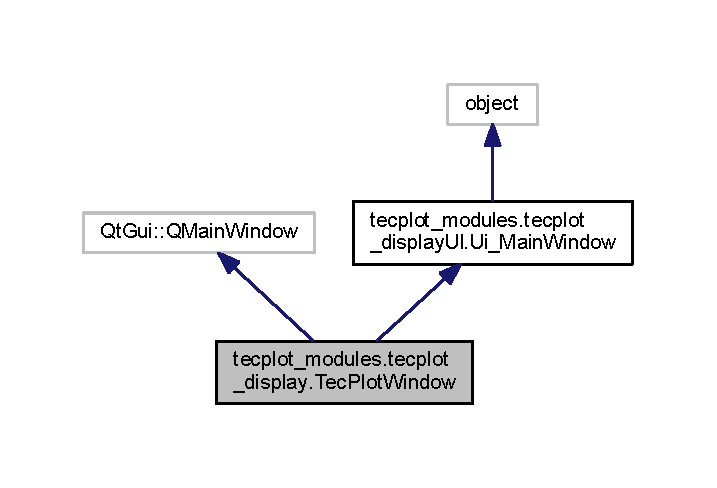
\includegraphics[width=344pt]{classtecplot__modules_1_1tecplot__display_1_1_tec_plot_window__inherit__graph}
\end{center}
\end{figure}
\subsection*{Public Member Functions}
\begin{DoxyCompactItemize}
\item 
def \hyperlink{classtecplot__modules_1_1tecplot__display_1_1_tec_plot_window_abc270dcf6e8aaa3a645ae0258c4a9e5e}{\+\_\+\+\_\+init\+\_\+\+\_\+} (self, parent=None, Output\+Viewer\+Widget=None)
\item 
def \hyperlink{classtecplot__modules_1_1tecplot__display_1_1_tec_plot_window_a6b4350a2c6ee537dba6bbe1549778636}{open\+Tecplot} (self, tecplot\+\_\+path=None)
\begin{DoxyCompactList}\small\item\em Calls the function for reading tecplot csv files of \hyperlink{classtecplot__modules_1_1tecplot__reader_1_1_tec_plot_core}{tecplot\+\_\+reader.\+Tec\+Plot\+Core}. \end{DoxyCompactList}\item 
def \hyperlink{classtecplot__modules_1_1tecplot__display_1_1_tec_plot_window_a62c9724fbeda8d8780e57559bada3282}{plot\+Function} (self)
\begin{DoxyCompactList}\small\item\em Calls tecplot\+\_\+core functions and saves it in instance variables and adjust graphics settings like padding. \end{DoxyCompactList}\item 
def \hyperlink{classtecplot__modules_1_1tecplot__display_1_1_tec_plot_window_ae792d997329b65cfed0b8a0a5feaa1a2}{tecplot\+Display\+\_\+1} (self)
\begin{DoxyCompactList}\small\item\em Methods that are going to be called by the the Tecplot\+Widget. \end{DoxyCompactList}\item 
def \hyperlink{classtecplot__modules_1_1tecplot__display_1_1_tec_plot_window_aec1f3f862b488e5f66161ca7241908c1}{tecplot\+Display\+\_\+2} (self)
\begin{DoxyCompactList}\small\item\em Methods that are going to be called by the the Tecplot\+Widget. \end{DoxyCompactList}\item 
def \hyperlink{classtecplot__modules_1_1tecplot__display_1_1_tec_plot_window_ae29c235476c3ca1ff19f4b933b86ed86}{tecplot\+Display\+\_\+3} (self)
\begin{DoxyCompactList}\small\item\em Methods that are going to be called by the the Tecplot\+Widget. \end{DoxyCompactList}\item 
def \hyperlink{classtecplot__modules_1_1tecplot__display_1_1_tec_plot_window_acdc9dc387494507084a2ab2cc0c8d9ac}{tecplot\+Display\+\_\+4} (self)
\begin{DoxyCompactList}\small\item\em Methods that are going to be called by the the Tecplot\+Widget. \end{DoxyCompactList}\item 
def \hyperlink{classtecplot__modules_1_1tecplot__display_1_1_tec_plot_window_ad80163041f7884f536d1421860c4adc2}{set\+Neutral} (self)
\begin{DoxyCompactList}\small\item\em Toggles tecplot display to neutral. \end{DoxyCompactList}\item 
def \hyperlink{classtecplot__modules_1_1tecplot__display_1_1_tec_plot_window_ae50e0f3c4051d791ed30a2e9de5233ea}{set\+Visibility} (self)
\begin{DoxyCompactList}\small\item\em Toggles tecplot display to visible or invisible for the selected case. \end{DoxyCompactList}\end{DoxyCompactItemize}
\subsection*{Public Attributes}
\begin{DoxyCompactItemize}
\item 
\hyperlink{classtecplot__modules_1_1tecplot__display_1_1_tec_plot_window_a97bc6a6c7074f874028cd2afbbad4082}{tecplot\+\_\+blade\+\_\+plotlines}
\item 
\hyperlink{classtecplot__modules_1_1tecplot__display_1_1_tec_plot_window_a103d285631a0d45198d834c8a98cf72a}{tecplot\+\_\+stream\+\_\+plotlines}
\item 
\hyperlink{classtecplot__modules_1_1tecplot__display_1_1_tec_plot_window_a20a9b77de151d414f78ab14a5ee30143}{tecplot\+\_\+profile\+\_\+plotlines}
\item 
\hyperlink{classtecplot__modules_1_1tecplot__display_1_1_tec_plot_window_ad430a4835103d6c1e22b1d81a829bc74}{tecplot\+\_\+mean\+\_\+plotlines}
\item 
\hyperlink{classtecplot__modules_1_1tecplot__display_1_1_tec_plot_window_a552371e32854caef73cb7386140ebab8}{tecplot\+\_\+meanbeta\+\_\+plotlines}
\item 
\hyperlink{classtecplot__modules_1_1tecplot__display_1_1_tec_plot_window_a3291e8bf0c5c69a20e3e9299dc363db2}{tecplot\+\_\+thickness\+\_\+plotlines}
\item 
\hyperlink{classtecplot__modules_1_1tecplot__display_1_1_tec_plot_window_a03539a28f4d15d303da92341074ab6b6}{op\+\_\+viewer}
\item 
\hyperlink{classtecplot__modules_1_1tecplot__display_1_1_tec_plot_window_a7d3fabc52fc4c2d52b9aa4efea25131a}{core}
\end{DoxyCompactItemize}


\subsection{Detailed Description}
Class for creating a G\+UI for the Blade\+Py Tecplot\+Viewer Widget. 

A object of this class will be created and integrated to the Output\+Viewer. This class has the function of displaying tecplot graphics, and managing its appearance in the functions \hyperlink{classtecplot__modules_1_1tecplot__display_1_1_tec_plot_window_ae50e0f3c4051d791ed30a2e9de5233ea}{set\+Visibility()} and \hyperlink{classtecplot__modules_1_1tecplot__display_1_1_tec_plot_window_ad80163041f7884f536d1421860c4adc2}{set\+Neutral()}. The padding, label and adjustments are made when plotting in \hyperlink{classtecplot__modules_1_1tecplot__display_1_1_tec_plot_window_a62c9724fbeda8d8780e57559bada3282}{plot\+Function()}. This object instantiates composition association object of \hyperlink{classtecplot__modules_1_1tecplot__reader_1_1_tec_plot_core}{tecplot\+\_\+reader.\+Tec\+Plot\+Core} class. The object of this class is used for reading tecplot csv files.

\hyperlink{classtecplot__modules_1_1tecplot__display_1_1_tec_plot_window_a62c9724fbeda8d8780e57559bada3282}{plot\+Function()} actually has the objective of directing the plots to the right canvas. The plotting and line creation are in fact made in methods \hyperlink{classtecplot__modules_1_1tecplot__display_1_1_tec_plot_window_ae792d997329b65cfed0b8a0a5feaa1a2}{tecplot\+Display\+\_\+1()}, \hyperlink{classtecplot__modules_1_1tecplot__display_1_1_tec_plot_window_aec1f3f862b488e5f66161ca7241908c1}{tecplot\+Display\+\_\+2()}, \hyperlink{classtecplot__modules_1_1tecplot__display_1_1_tec_plot_window_ae29c235476c3ca1ff19f4b933b86ed86}{tecplot\+Display\+\_\+3()}, and \hyperlink{classtecplot__modules_1_1tecplot__display_1_1_tec_plot_window_acdc9dc387494507084a2ab2cc0c8d9ac}{tecplot\+Display\+\_\+4()}.

The reason for having four different methods for plotting is the fact that each canvas has it own rule for plotting.

This class is responsible for adding functions to the inherited \hyperlink{classtecplot__modules_1_1tecplot__display_u_i_1_1_ui___main_window}{tecplot\+\_\+display\+U\+I.\+Ui\+\_\+\+Main\+Window} function-\/less layout created in Qt Designer. 

\subsection{Constructor \& Destructor Documentation}
\hypertarget{classtecplot__modules_1_1tecplot__display_1_1_tec_plot_window_abc270dcf6e8aaa3a645ae0258c4a9e5e}{}\label{classtecplot__modules_1_1tecplot__display_1_1_tec_plot_window_abc270dcf6e8aaa3a645ae0258c4a9e5e} 
\index{tecplot\+\_\+modules\+::tecplot\+\_\+display\+::\+Tec\+Plot\+Window@{tecplot\+\_\+modules\+::tecplot\+\_\+display\+::\+Tec\+Plot\+Window}!\+\_\+\+\_\+init\+\_\+\+\_\+@{\+\_\+\+\_\+init\+\_\+\+\_\+}}
\index{\+\_\+\+\_\+init\+\_\+\+\_\+@{\+\_\+\+\_\+init\+\_\+\+\_\+}!tecplot\+\_\+modules\+::tecplot\+\_\+display\+::\+Tec\+Plot\+Window@{tecplot\+\_\+modules\+::tecplot\+\_\+display\+::\+Tec\+Plot\+Window}}
\subsubsection{\texorpdfstring{\+\_\+\+\_\+init\+\_\+\+\_\+()}{\_\_init\_\_()}}
{\footnotesize\ttfamily def tecplot\+\_\+modules.\+tecplot\+\_\+display.\+Tec\+Plot\+Window.\+\_\+\+\_\+init\+\_\+\+\_\+ (\begin{DoxyParamCaption}\item[{}]{self,  }\item[{}]{parent = {\ttfamily None},  }\item[{}]{Output\+Viewer\+Widget = {\ttfamily None} }\end{DoxyParamCaption})}



\subsection{Member Function Documentation}
\hypertarget{classtecplot__modules_1_1tecplot__display_1_1_tec_plot_window_a6b4350a2c6ee537dba6bbe1549778636}{}\label{classtecplot__modules_1_1tecplot__display_1_1_tec_plot_window_a6b4350a2c6ee537dba6bbe1549778636} 
\index{tecplot\+\_\+modules\+::tecplot\+\_\+display\+::\+Tec\+Plot\+Window@{tecplot\+\_\+modules\+::tecplot\+\_\+display\+::\+Tec\+Plot\+Window}!open\+Tecplot@{open\+Tecplot}}
\index{open\+Tecplot@{open\+Tecplot}!tecplot\+\_\+modules\+::tecplot\+\_\+display\+::\+Tec\+Plot\+Window@{tecplot\+\_\+modules\+::tecplot\+\_\+display\+::\+Tec\+Plot\+Window}}
\subsubsection{\texorpdfstring{open\+Tecplot()}{openTecplot()}}
{\footnotesize\ttfamily def tecplot\+\_\+modules.\+tecplot\+\_\+display.\+Tec\+Plot\+Window.\+open\+Tecplot (\begin{DoxyParamCaption}\item[{}]{self,  }\item[{}]{tecplot\+\_\+path = {\ttfamily None} }\end{DoxyParamCaption})}



Calls the function for reading tecplot csv files of \hyperlink{classtecplot__modules_1_1tecplot__reader_1_1_tec_plot_core}{tecplot\+\_\+reader.\+Tec\+Plot\+Core}. 

Then calls \hyperlink{classtecplot__modules_1_1tecplot__display_1_1_tec_plot_window_a62c9724fbeda8d8780e57559bada3282}{plot\+Function()} to plot the read files.

\begin{DoxyReturn}{Returns}
None 
\end{DoxyReturn}
\hypertarget{classtecplot__modules_1_1tecplot__display_1_1_tec_plot_window_a62c9724fbeda8d8780e57559bada3282}{}\label{classtecplot__modules_1_1tecplot__display_1_1_tec_plot_window_a62c9724fbeda8d8780e57559bada3282} 
\index{tecplot\+\_\+modules\+::tecplot\+\_\+display\+::\+Tec\+Plot\+Window@{tecplot\+\_\+modules\+::tecplot\+\_\+display\+::\+Tec\+Plot\+Window}!plot\+Function@{plot\+Function}}
\index{plot\+Function@{plot\+Function}!tecplot\+\_\+modules\+::tecplot\+\_\+display\+::\+Tec\+Plot\+Window@{tecplot\+\_\+modules\+::tecplot\+\_\+display\+::\+Tec\+Plot\+Window}}
\subsubsection{\texorpdfstring{plot\+Function()}{plotFunction()}}
{\footnotesize\ttfamily def tecplot\+\_\+modules.\+tecplot\+\_\+display.\+Tec\+Plot\+Window.\+plot\+Function (\begin{DoxyParamCaption}\item[{}]{self }\end{DoxyParamCaption})}



Calls tecplot\+\_\+core functions and saves it in instance variables and adjust graphics settings like padding. 

\begin{DoxyReturn}{Returns}
None 
\end{DoxyReturn}
\hypertarget{classtecplot__modules_1_1tecplot__display_1_1_tec_plot_window_ad80163041f7884f536d1421860c4adc2}{}\label{classtecplot__modules_1_1tecplot__display_1_1_tec_plot_window_ad80163041f7884f536d1421860c4adc2} 
\index{tecplot\+\_\+modules\+::tecplot\+\_\+display\+::\+Tec\+Plot\+Window@{tecplot\+\_\+modules\+::tecplot\+\_\+display\+::\+Tec\+Plot\+Window}!set\+Neutral@{set\+Neutral}}
\index{set\+Neutral@{set\+Neutral}!tecplot\+\_\+modules\+::tecplot\+\_\+display\+::\+Tec\+Plot\+Window@{tecplot\+\_\+modules\+::tecplot\+\_\+display\+::\+Tec\+Plot\+Window}}
\subsubsection{\texorpdfstring{set\+Neutral()}{setNeutral()}}
{\footnotesize\ttfamily def tecplot\+\_\+modules.\+tecplot\+\_\+display.\+Tec\+Plot\+Window.\+set\+Neutral (\begin{DoxyParamCaption}\item[{}]{self,  }\item[{}]{None }\end{DoxyParamCaption})}



Toggles tecplot display to neutral. 

Sets to neutral mode -\/ black and dashed lines -\/ or to standard for the selected case. For hub and shroud there is no neutral state. Only stream lines will become dashed a blacked.

\begin{DoxyReturn}{Returns}
None 
\end{DoxyReturn}
\hypertarget{classtecplot__modules_1_1tecplot__display_1_1_tec_plot_window_ae50e0f3c4051d791ed30a2e9de5233ea}{}\label{classtecplot__modules_1_1tecplot__display_1_1_tec_plot_window_ae50e0f3c4051d791ed30a2e9de5233ea} 
\index{tecplot\+\_\+modules\+::tecplot\+\_\+display\+::\+Tec\+Plot\+Window@{tecplot\+\_\+modules\+::tecplot\+\_\+display\+::\+Tec\+Plot\+Window}!set\+Visibility@{set\+Visibility}}
\index{set\+Visibility@{set\+Visibility}!tecplot\+\_\+modules\+::tecplot\+\_\+display\+::\+Tec\+Plot\+Window@{tecplot\+\_\+modules\+::tecplot\+\_\+display\+::\+Tec\+Plot\+Window}}
\subsubsection{\texorpdfstring{set\+Visibility()}{setVisibility()}}
{\footnotesize\ttfamily def tecplot\+\_\+modules.\+tecplot\+\_\+display.\+Tec\+Plot\+Window.\+set\+Visibility (\begin{DoxyParamCaption}\item[{}]{self,  }\item[{}]{None }\end{DoxyParamCaption})}



Toggles tecplot display to visible or invisible for the selected case. 

\begin{DoxyReturn}{Returns}
None 
\end{DoxyReturn}
\hypertarget{classtecplot__modules_1_1tecplot__display_1_1_tec_plot_window_ae792d997329b65cfed0b8a0a5feaa1a2}{}\label{classtecplot__modules_1_1tecplot__display_1_1_tec_plot_window_ae792d997329b65cfed0b8a0a5feaa1a2} 
\index{tecplot\+\_\+modules\+::tecplot\+\_\+display\+::\+Tec\+Plot\+Window@{tecplot\+\_\+modules\+::tecplot\+\_\+display\+::\+Tec\+Plot\+Window}!tecplot\+Display\+\_\+1@{tecplot\+Display\+\_\+1}}
\index{tecplot\+Display\+\_\+1@{tecplot\+Display\+\_\+1}!tecplot\+\_\+modules\+::tecplot\+\_\+display\+::\+Tec\+Plot\+Window@{tecplot\+\_\+modules\+::tecplot\+\_\+display\+::\+Tec\+Plot\+Window}}
\subsubsection{\texorpdfstring{tecplot\+Display\+\_\+1()}{tecplotDisplay\_1()}}
{\footnotesize\ttfamily def tecplot\+\_\+modules.\+tecplot\+\_\+display.\+Tec\+Plot\+Window.\+tecplot\+Display\+\_\+1 (\begin{DoxyParamCaption}\item[{}]{self }\end{DoxyParamCaption})}



Methods that are going to be called by the the Tecplot\+Widget. 

\begin{DoxyReturn}{Returns}
\mbox{[}list\mbox{]} List of blade plotlines and list of lists of Stream Lines plotlines 
\end{DoxyReturn}
\hypertarget{classtecplot__modules_1_1tecplot__display_1_1_tec_plot_window_aec1f3f862b488e5f66161ca7241908c1}{}\label{classtecplot__modules_1_1tecplot__display_1_1_tec_plot_window_aec1f3f862b488e5f66161ca7241908c1} 
\index{tecplot\+\_\+modules\+::tecplot\+\_\+display\+::\+Tec\+Plot\+Window@{tecplot\+\_\+modules\+::tecplot\+\_\+display\+::\+Tec\+Plot\+Window}!tecplot\+Display\+\_\+2@{tecplot\+Display\+\_\+2}}
\index{tecplot\+Display\+\_\+2@{tecplot\+Display\+\_\+2}!tecplot\+\_\+modules\+::tecplot\+\_\+display\+::\+Tec\+Plot\+Window@{tecplot\+\_\+modules\+::tecplot\+\_\+display\+::\+Tec\+Plot\+Window}}
\subsubsection{\texorpdfstring{tecplot\+Display\+\_\+2()}{tecplotDisplay\_2()}}
{\footnotesize\ttfamily def tecplot\+\_\+modules.\+tecplot\+\_\+display.\+Tec\+Plot\+Window.\+tecplot\+Display\+\_\+2 (\begin{DoxyParamCaption}\item[{}]{self }\end{DoxyParamCaption})}



Methods that are going to be called by the the Tecplot\+Widget. 

\begin{DoxyReturn}{Returns}
\mbox{[}list\mbox{]} List of lists of blade profiles plotlines and list of lists of Mean Lines plotlines 
\end{DoxyReturn}
\hypertarget{classtecplot__modules_1_1tecplot__display_1_1_tec_plot_window_ae29c235476c3ca1ff19f4b933b86ed86}{}\label{classtecplot__modules_1_1tecplot__display_1_1_tec_plot_window_ae29c235476c3ca1ff19f4b933b86ed86} 
\index{tecplot\+\_\+modules\+::tecplot\+\_\+display\+::\+Tec\+Plot\+Window@{tecplot\+\_\+modules\+::tecplot\+\_\+display\+::\+Tec\+Plot\+Window}!tecplot\+Display\+\_\+3@{tecplot\+Display\+\_\+3}}
\index{tecplot\+Display\+\_\+3@{tecplot\+Display\+\_\+3}!tecplot\+\_\+modules\+::tecplot\+\_\+display\+::\+Tec\+Plot\+Window@{tecplot\+\_\+modules\+::tecplot\+\_\+display\+::\+Tec\+Plot\+Window}}
\subsubsection{\texorpdfstring{tecplot\+Display\+\_\+3()}{tecplotDisplay\_3()}}
{\footnotesize\ttfamily def tecplot\+\_\+modules.\+tecplot\+\_\+display.\+Tec\+Plot\+Window.\+tecplot\+Display\+\_\+3 (\begin{DoxyParamCaption}\item[{}]{self }\end{DoxyParamCaption})}



Methods that are going to be called by the the Tecplot\+Widget. 

\begin{DoxyReturn}{Returns}
\mbox{[}list\mbox{]} List of lists of thickness plotlines 
\end{DoxyReturn}
\hypertarget{classtecplot__modules_1_1tecplot__display_1_1_tec_plot_window_acdc9dc387494507084a2ab2cc0c8d9ac}{}\label{classtecplot__modules_1_1tecplot__display_1_1_tec_plot_window_acdc9dc387494507084a2ab2cc0c8d9ac} 
\index{tecplot\+\_\+modules\+::tecplot\+\_\+display\+::\+Tec\+Plot\+Window@{tecplot\+\_\+modules\+::tecplot\+\_\+display\+::\+Tec\+Plot\+Window}!tecplot\+Display\+\_\+4@{tecplot\+Display\+\_\+4}}
\index{tecplot\+Display\+\_\+4@{tecplot\+Display\+\_\+4}!tecplot\+\_\+modules\+::tecplot\+\_\+display\+::\+Tec\+Plot\+Window@{tecplot\+\_\+modules\+::tecplot\+\_\+display\+::\+Tec\+Plot\+Window}}
\subsubsection{\texorpdfstring{tecplot\+Display\+\_\+4()}{tecplotDisplay\_4()}}
{\footnotesize\ttfamily def tecplot\+\_\+modules.\+tecplot\+\_\+display.\+Tec\+Plot\+Window.\+tecplot\+Display\+\_\+4 (\begin{DoxyParamCaption}\item[{}]{self }\end{DoxyParamCaption})}



Methods that are going to be called by the the Tecplot\+Widget. 

\begin{DoxyReturn}{Returns}
\mbox{[}list\mbox{]} List of lists of thickness plotlines 
\end{DoxyReturn}


\subsection{Member Data Documentation}
\hypertarget{classtecplot__modules_1_1tecplot__display_1_1_tec_plot_window_a7d3fabc52fc4c2d52b9aa4efea25131a}{}\label{classtecplot__modules_1_1tecplot__display_1_1_tec_plot_window_a7d3fabc52fc4c2d52b9aa4efea25131a} 
\index{tecplot\+\_\+modules\+::tecplot\+\_\+display\+::\+Tec\+Plot\+Window@{tecplot\+\_\+modules\+::tecplot\+\_\+display\+::\+Tec\+Plot\+Window}!core@{core}}
\index{core@{core}!tecplot\+\_\+modules\+::tecplot\+\_\+display\+::\+Tec\+Plot\+Window@{tecplot\+\_\+modules\+::tecplot\+\_\+display\+::\+Tec\+Plot\+Window}}
\subsubsection{\texorpdfstring{core}{core}}
{\footnotesize\ttfamily tecplot\+\_\+modules.\+tecplot\+\_\+display.\+Tec\+Plot\+Window.\+core}

\hypertarget{classtecplot__modules_1_1tecplot__display_1_1_tec_plot_window_a03539a28f4d15d303da92341074ab6b6}{}\label{classtecplot__modules_1_1tecplot__display_1_1_tec_plot_window_a03539a28f4d15d303da92341074ab6b6} 
\index{tecplot\+\_\+modules\+::tecplot\+\_\+display\+::\+Tec\+Plot\+Window@{tecplot\+\_\+modules\+::tecplot\+\_\+display\+::\+Tec\+Plot\+Window}!op\+\_\+viewer@{op\+\_\+viewer}}
\index{op\+\_\+viewer@{op\+\_\+viewer}!tecplot\+\_\+modules\+::tecplot\+\_\+display\+::\+Tec\+Plot\+Window@{tecplot\+\_\+modules\+::tecplot\+\_\+display\+::\+Tec\+Plot\+Window}}
\subsubsection{\texorpdfstring{op\+\_\+viewer}{op\_viewer}}
{\footnotesize\ttfamily tecplot\+\_\+modules.\+tecplot\+\_\+display.\+Tec\+Plot\+Window.\+op\+\_\+viewer}

\hypertarget{classtecplot__modules_1_1tecplot__display_1_1_tec_plot_window_a97bc6a6c7074f874028cd2afbbad4082}{}\label{classtecplot__modules_1_1tecplot__display_1_1_tec_plot_window_a97bc6a6c7074f874028cd2afbbad4082} 
\index{tecplot\+\_\+modules\+::tecplot\+\_\+display\+::\+Tec\+Plot\+Window@{tecplot\+\_\+modules\+::tecplot\+\_\+display\+::\+Tec\+Plot\+Window}!tecplot\+\_\+blade\+\_\+plotlines@{tecplot\+\_\+blade\+\_\+plotlines}}
\index{tecplot\+\_\+blade\+\_\+plotlines@{tecplot\+\_\+blade\+\_\+plotlines}!tecplot\+\_\+modules\+::tecplot\+\_\+display\+::\+Tec\+Plot\+Window@{tecplot\+\_\+modules\+::tecplot\+\_\+display\+::\+Tec\+Plot\+Window}}
\subsubsection{\texorpdfstring{tecplot\+\_\+blade\+\_\+plotlines}{tecplot\_blade\_plotlines}}
{\footnotesize\ttfamily tecplot\+\_\+modules.\+tecplot\+\_\+display.\+Tec\+Plot\+Window.\+tecplot\+\_\+blade\+\_\+plotlines}

\hypertarget{classtecplot__modules_1_1tecplot__display_1_1_tec_plot_window_ad430a4835103d6c1e22b1d81a829bc74}{}\label{classtecplot__modules_1_1tecplot__display_1_1_tec_plot_window_ad430a4835103d6c1e22b1d81a829bc74} 
\index{tecplot\+\_\+modules\+::tecplot\+\_\+display\+::\+Tec\+Plot\+Window@{tecplot\+\_\+modules\+::tecplot\+\_\+display\+::\+Tec\+Plot\+Window}!tecplot\+\_\+mean\+\_\+plotlines@{tecplot\+\_\+mean\+\_\+plotlines}}
\index{tecplot\+\_\+mean\+\_\+plotlines@{tecplot\+\_\+mean\+\_\+plotlines}!tecplot\+\_\+modules\+::tecplot\+\_\+display\+::\+Tec\+Plot\+Window@{tecplot\+\_\+modules\+::tecplot\+\_\+display\+::\+Tec\+Plot\+Window}}
\subsubsection{\texorpdfstring{tecplot\+\_\+mean\+\_\+plotlines}{tecplot\_mean\_plotlines}}
{\footnotesize\ttfamily tecplot\+\_\+modules.\+tecplot\+\_\+display.\+Tec\+Plot\+Window.\+tecplot\+\_\+mean\+\_\+plotlines}

\hypertarget{classtecplot__modules_1_1tecplot__display_1_1_tec_plot_window_a552371e32854caef73cb7386140ebab8}{}\label{classtecplot__modules_1_1tecplot__display_1_1_tec_plot_window_a552371e32854caef73cb7386140ebab8} 
\index{tecplot\+\_\+modules\+::tecplot\+\_\+display\+::\+Tec\+Plot\+Window@{tecplot\+\_\+modules\+::tecplot\+\_\+display\+::\+Tec\+Plot\+Window}!tecplot\+\_\+meanbeta\+\_\+plotlines@{tecplot\+\_\+meanbeta\+\_\+plotlines}}
\index{tecplot\+\_\+meanbeta\+\_\+plotlines@{tecplot\+\_\+meanbeta\+\_\+plotlines}!tecplot\+\_\+modules\+::tecplot\+\_\+display\+::\+Tec\+Plot\+Window@{tecplot\+\_\+modules\+::tecplot\+\_\+display\+::\+Tec\+Plot\+Window}}
\subsubsection{\texorpdfstring{tecplot\+\_\+meanbeta\+\_\+plotlines}{tecplot\_meanbeta\_plotlines}}
{\footnotesize\ttfamily tecplot\+\_\+modules.\+tecplot\+\_\+display.\+Tec\+Plot\+Window.\+tecplot\+\_\+meanbeta\+\_\+plotlines}

\hypertarget{classtecplot__modules_1_1tecplot__display_1_1_tec_plot_window_a20a9b77de151d414f78ab14a5ee30143}{}\label{classtecplot__modules_1_1tecplot__display_1_1_tec_plot_window_a20a9b77de151d414f78ab14a5ee30143} 
\index{tecplot\+\_\+modules\+::tecplot\+\_\+display\+::\+Tec\+Plot\+Window@{tecplot\+\_\+modules\+::tecplot\+\_\+display\+::\+Tec\+Plot\+Window}!tecplot\+\_\+profile\+\_\+plotlines@{tecplot\+\_\+profile\+\_\+plotlines}}
\index{tecplot\+\_\+profile\+\_\+plotlines@{tecplot\+\_\+profile\+\_\+plotlines}!tecplot\+\_\+modules\+::tecplot\+\_\+display\+::\+Tec\+Plot\+Window@{tecplot\+\_\+modules\+::tecplot\+\_\+display\+::\+Tec\+Plot\+Window}}
\subsubsection{\texorpdfstring{tecplot\+\_\+profile\+\_\+plotlines}{tecplot\_profile\_plotlines}}
{\footnotesize\ttfamily tecplot\+\_\+modules.\+tecplot\+\_\+display.\+Tec\+Plot\+Window.\+tecplot\+\_\+profile\+\_\+plotlines}

\hypertarget{classtecplot__modules_1_1tecplot__display_1_1_tec_plot_window_a103d285631a0d45198d834c8a98cf72a}{}\label{classtecplot__modules_1_1tecplot__display_1_1_tec_plot_window_a103d285631a0d45198d834c8a98cf72a} 
\index{tecplot\+\_\+modules\+::tecplot\+\_\+display\+::\+Tec\+Plot\+Window@{tecplot\+\_\+modules\+::tecplot\+\_\+display\+::\+Tec\+Plot\+Window}!tecplot\+\_\+stream\+\_\+plotlines@{tecplot\+\_\+stream\+\_\+plotlines}}
\index{tecplot\+\_\+stream\+\_\+plotlines@{tecplot\+\_\+stream\+\_\+plotlines}!tecplot\+\_\+modules\+::tecplot\+\_\+display\+::\+Tec\+Plot\+Window@{tecplot\+\_\+modules\+::tecplot\+\_\+display\+::\+Tec\+Plot\+Window}}
\subsubsection{\texorpdfstring{tecplot\+\_\+stream\+\_\+plotlines}{tecplot\_stream\_plotlines}}
{\footnotesize\ttfamily tecplot\+\_\+modules.\+tecplot\+\_\+display.\+Tec\+Plot\+Window.\+tecplot\+\_\+stream\+\_\+plotlines}

\hypertarget{classtecplot__modules_1_1tecplot__display_1_1_tec_plot_window_a3291e8bf0c5c69a20e3e9299dc363db2}{}\label{classtecplot__modules_1_1tecplot__display_1_1_tec_plot_window_a3291e8bf0c5c69a20e3e9299dc363db2} 
\index{tecplot\+\_\+modules\+::tecplot\+\_\+display\+::\+Tec\+Plot\+Window@{tecplot\+\_\+modules\+::tecplot\+\_\+display\+::\+Tec\+Plot\+Window}!tecplot\+\_\+thickness\+\_\+plotlines@{tecplot\+\_\+thickness\+\_\+plotlines}}
\index{tecplot\+\_\+thickness\+\_\+plotlines@{tecplot\+\_\+thickness\+\_\+plotlines}!tecplot\+\_\+modules\+::tecplot\+\_\+display\+::\+Tec\+Plot\+Window@{tecplot\+\_\+modules\+::tecplot\+\_\+display\+::\+Tec\+Plot\+Window}}
\subsubsection{\texorpdfstring{tecplot\+\_\+thickness\+\_\+plotlines}{tecplot\_thickness\_plotlines}}
{\footnotesize\ttfamily tecplot\+\_\+modules.\+tecplot\+\_\+display.\+Tec\+Plot\+Window.\+tecplot\+\_\+thickness\+\_\+plotlines}



The documentation for this class was generated from the following file\+:\begin{DoxyCompactItemize}
\item 
\hyperlink{tecplot__display_8py}{tecplot\+\_\+display.\+py}\end{DoxyCompactItemize}

\hypertarget{classoutput__viewer_u_i_1_1_ui___main_window}{}\section{output\+\_\+viewer\+U\+I.\+Ui\+\_\+\+Main\+Window Class Reference}
\label{classoutput__viewer_u_i_1_1_ui___main_window}\index{output\+\_\+viewer\+U\+I.\+Ui\+\_\+\+Main\+Window@{output\+\_\+viewer\+U\+I.\+Ui\+\_\+\+Main\+Window}}


Inheritance diagram for output\+\_\+viewer\+U\+I.\+Ui\+\_\+\+Main\+Window\+:\nopagebreak
\begin{figure}[H]
\begin{center}
\leavevmode
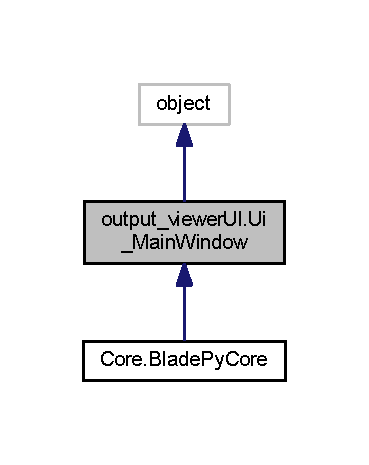
\includegraphics[width=177pt]{classoutput__viewer_u_i_1_1_ui___main_window__inherit__graph}
\end{center}
\end{figure}
\subsection*{Public Member Functions}
\begin{DoxyCompactItemize}
\item 
def \hyperlink{classoutput__viewer_u_i_1_1_ui___main_window_a2a9ce5c092ffe5a4e4cabb341be7ceb4}{setup\+Ui} (self, \hyperlink{namespaceoutput__viewer_u_i_a95763e93bffcc3d9bda7ae977c5c2c4e}{Main\+Window})
\item 
def \hyperlink{classoutput__viewer_u_i_1_1_ui___main_window_a96efd9219a406e801e268b7add32cb78}{retranslate\+Ui} (self, \hyperlink{namespaceoutput__viewer_u_i_a95763e93bffcc3d9bda7ae977c5c2c4e}{Main\+Window})
\end{DoxyCompactItemize}
\subsection*{Public Attributes}
\begin{DoxyCompactItemize}
\item 
\hyperlink{classoutput__viewer_u_i_1_1_ui___main_window_a2a323cc6e8e271345a42cb3342820d3b}{centralwidget}
\item 
\hyperlink{classoutput__viewer_u_i_1_1_ui___main_window_a84fbe4915db0698d6779bab59a55b20a}{centralwidget\+\_\+hl}
\item 
\hyperlink{classoutput__viewer_u_i_1_1_ui___main_window_a840ced767970f65402ef894fb5fcc3f3}{statusbar}
\item 
\hyperlink{classoutput__viewer_u_i_1_1_ui___main_window_aa1bd7f326134cd7873cadb8a3e89d866}{ui\+\_\+file\+\_\+toolbar}
\item 
\hyperlink{classoutput__viewer_u_i_1_1_ui___main_window_ada862a642c3a9c359564a67539047d12}{ui\+\_\+view\+\_\+toolbar}
\item 
\hyperlink{classoutput__viewer_u_i_1_1_ui___main_window_aaa6b736b767520bf24e89cfaf72ae15f}{ui\+\_\+treeview\+\_\+dockW}
\item 
\hyperlink{classoutput__viewer_u_i_1_1_ui___main_window_ae11b22f4f511169e79dd98b5e886890d}{ui\+\_\+treeview\+\_\+dockcontents}
\item 
\hyperlink{classoutput__viewer_u_i_1_1_ui___main_window_a6bf94b92513eaa3732c9dfec3f32697c}{ui\+\_\+treeview\+\_\+dockcontents\+\_\+vl}
\item 
\hyperlink{classoutput__viewer_u_i_1_1_ui___main_window_a43692c1dd9ca5ac7d3b92aefb56d3a47}{ui\+\_\+case\+\_\+treeview}
\item 
\hyperlink{classoutput__viewer_u_i_1_1_ui___main_window_ab7e73e16ab3e6b27d3d50400bc8adaa9}{ui\+\_\+subcase\+\_\+list}
\item 
\hyperlink{classoutput__viewer_u_i_1_1_ui___main_window_ab81dbfc042d78295a9c868c026846575}{ui\+\_\+deletecase\+\_\+btn}
\item 
\hyperlink{classoutput__viewer_u_i_1_1_ui___main_window_a8507133b9e49326677916d0b69587180}{ui\+\_\+propertiestools\+\_\+dockW}
\item 
\hyperlink{classoutput__viewer_u_i_1_1_ui___main_window_a26eae51ef2c81417b401501bca6ce10a}{ui\+\_\+propertiestools\+\_\+dockcontents}
\item 
\hyperlink{classoutput__viewer_u_i_1_1_ui___main_window_a83c00b5893231c0eba98a9e8e22ac09c}{ui\+\_\+propertiestools\+\_\+dockcontents\+\_\+gl}
\item 
\hyperlink{classoutput__viewer_u_i_1_1_ui___main_window_a0b802c9e05ee17be9d7fd6a867b2aa0f}{ui\+\_\+selectedcase\+\_\+edit}
\item 
\hyperlink{classoutput__viewer_u_i_1_1_ui___main_window_ab3983cab5036a720f91ae2ae62374f73}{ui\+\_\+zoom\+\_\+lbl}
\item 
\hyperlink{classoutput__viewer_u_i_1_1_ui___main_window_aa660273332cc5da8d46ae6e465323eda}{ui\+\_\+shapeappearance\+\_\+groupbox}
\item 
\hyperlink{classoutput__viewer_u_i_1_1_ui___main_window_a04a31fbb2f456070dfd32b6f122923b6}{ui\+\_\+shape\+\_\+appearance\+\_\+groupbox\+\_\+gl}
\item 
\hyperlink{classoutput__viewer_u_i_1_1_ui___main_window_a2b9029cd44541c9b09508f9cddbbffd7}{ui\+\_\+shape\+\_\+setcolor\+\_\+btn}
\item 
\hyperlink{classoutput__viewer_u_i_1_1_ui___main_window_a29e4e3e1bc1a96b5b5970f03ccdc3258}{ui\+\_\+shape\+\_\+settransparency\+\_\+btn}
\item 
\hyperlink{classoutput__viewer_u_i_1_1_ui___main_window_a0ad9bf35073cf45204d5ddca0156df53}{ui\+\_\+shape\+\_\+transparency\+\_\+dspn}
\item 
\hyperlink{classoutput__viewer_u_i_1_1_ui___main_window_a4ee4bf54cb958bebdc43e8598dcdd459}{ui\+\_\+shape\+\_\+quality\+\_\+btn}
\item 
\hyperlink{classoutput__viewer_u_i_1_1_ui___main_window_a091706f3093b19dadcf896b4fc354dc1}{ui\+\_\+shape\+\_\+quality\+\_\+dspn}
\item 
\hyperlink{classoutput__viewer_u_i_1_1_ui___main_window_a6412380402adf28d010e459b538c97be}{ui\+\_\+shape\+\_\+setcolor\+\_\+combo}
\item 
\hyperlink{classoutput__viewer_u_i_1_1_ui___main_window_af27038ec976b97c8007f5914afb2f4ed}{ui\+\_\+shape\+\_\+hide\+\_\+btn}
\item 
\hyperlink{classoutput__viewer_u_i_1_1_ui___main_window_ae8028f5880df8b13414eba6f474a3aee}{ui\+\_\+shape\+\_\+display\+\_\+btn}
\item 
\hyperlink{classoutput__viewer_u_i_1_1_ui___main_window_a1fc23acd26cd3067a21b1814e61be00e}{ui\+\_\+shape\+\_\+transformation\+\_\+groupbox}
\item 
\hyperlink{classoutput__viewer_u_i_1_1_ui___main_window_aebd41dcf93d9fad7a4dca658b1889a44}{ui\+\_\+shape\+\_\+transformation\+\_\+groupbox\+\_\+gl}
\item 
\hyperlink{classoutput__viewer_u_i_1_1_ui___main_window_a692312c2b09073353e2bfb7432092583}{ui\+\_\+ydispl\+\_\+lbl}
\item 
\hyperlink{classoutput__viewer_u_i_1_1_ui___main_window_aa28c70006d121bac80ae12022d751fd9}{ui\+\_\+shape\+\_\+tetarotat\+\_\+dspn}
\item 
\hyperlink{classoutput__viewer_u_i_1_1_ui___main_window_ab8782732fd9dcbabe62718d4fd1eb451}{ui\+\_\+shape\+\_\+rotataxis\+\_\+combo}
\item 
\hyperlink{classoutput__viewer_u_i_1_1_ui___main_window_a9f2714b1287e94beaec813c4859a76ed}{ui\+\_\+axisrotat\+\_\+lbl}
\item 
\hyperlink{classoutput__viewer_u_i_1_1_ui___main_window_a9a614d93a0e921aa5e8e2692269ea93e}{ui\+\_\+shape\+\_\+xdispl\+\_\+dspn}
\item 
\hyperlink{classoutput__viewer_u_i_1_1_ui___main_window_a365b7f614170273dffc60d90f68e7b50}{ui\+\_\+xdispl\+\_\+lbl}
\item 
\hyperlink{classoutput__viewer_u_i_1_1_ui___main_window_a6393abac6ef3d14dd99f90c2038ce668}{ui\+\_\+zdispl\+\_\+lbl}
\item 
\hyperlink{classoutput__viewer_u_i_1_1_ui___main_window_ac2513163c4489ee11aa128f248ac25bc}{ui\+\_\+shape\+\_\+zdispl\+\_\+dspn}
\item 
\hyperlink{classoutput__viewer_u_i_1_1_ui___main_window_a6d782a6f55b193b51dbc457441b6bb6b}{ui\+\_\+shape\+\_\+ydispl\+\_\+dspn}
\item 
\hyperlink{classoutput__viewer_u_i_1_1_ui___main_window_a7463f5748bcd87fed9c7aa83d70d7b4c}{ui\+\_\+shape\+\_\+settranslation\+\_\+btn}
\item 
\hyperlink{classoutput__viewer_u_i_1_1_ui___main_window_a1ed7a735f4879c9335af120f50f99554}{ui\+\_\+tecplot\+\_\+control\+\_\+groupbox}
\item 
\hyperlink{classoutput__viewer_u_i_1_1_ui___main_window_ae4ccda1baa67cbf1b90aeaf28c792f52}{horizontal\+Layout}
\item 
\hyperlink{classoutput__viewer_u_i_1_1_ui___main_window_a7efc66f5379a990bb2d613efad8af792}{ui\+\_\+tecplot\+\_\+setinvisible\+\_\+btn}
\item 
\hyperlink{classoutput__viewer_u_i_1_1_ui___main_window_a7a5d64ed74f4a2a389cfbd88660084ea}{ui\+\_\+tecplot\+\_\+setneutral\+\_\+btn}
\item 
\hyperlink{classoutput__viewer_u_i_1_1_ui___main_window_aab2a02b2ad9ef412370fa6ce21aba778}{ui\+\_\+display\+\_\+zoomfactor\+\_\+dspn}
\item 
\hyperlink{classoutput__viewer_u_i_1_1_ui___main_window_a6ac6813ef0dc08cb729b515d9edfd656}{ui\+\_\+tecplotgraphics\+\_\+dockW}
\item 
\hyperlink{classoutput__viewer_u_i_1_1_ui___main_window_a833a8408dc99f9eedbb331e8e360bdf5}{ui\+\_\+tecplotgraphics\+\_\+dockcontents}
\item 
\hyperlink{classoutput__viewer_u_i_1_1_ui___main_window_a9937dfdabe6438f3bfec3ba0c6976557}{ui\+\_\+tecplotgraphics\+\_\+dockcontents\+\_\+vl}
\item 
\hyperlink{classoutput__viewer_u_i_1_1_ui___main_window_a7e3ee3296fa5786336d90635c2442045}{ui\+\_\+tecplot\+\_\+widget}
\item 
\hyperlink{classoutput__viewer_u_i_1_1_ui___main_window_a617fa074367d63edd758567a5d67b398}{ui\+\_\+tecplot\+\_\+widget\+\_\+vl}
\item 
\hyperlink{classoutput__viewer_u_i_1_1_ui___main_window_afbd7bdb7c0f0d9d24bad52a80454d101}{ui\+\_\+tecplot\+\_\+toolbar}
\item 
\hyperlink{classoutput__viewer_u_i_1_1_ui___main_window_a34720910fa97b9e65de72cbee6a12803}{ui\+\_\+settings\+\_\+toolbar}
\item 
\hyperlink{classoutput__viewer_u_i_1_1_ui___main_window_a265e28ccad6c1cd4a94a22965fe6c536}{menubar}
\item 
\hyperlink{classoutput__viewer_u_i_1_1_ui___main_window_ad42c5a1028285e160bfb9eb048cd245b}{ui\+\_\+file\+\_\+menu\+\_\+}
\item 
\hyperlink{classoutput__viewer_u_i_1_1_ui___main_window_a791ff2e9d4693638b8e5220f53f1b8d2}{ui\+\_\+edit\+\_\+menu}
\item 
\hyperlink{classoutput__viewer_u_i_1_1_ui___main_window_aaf13351c59caceedfc932c46217b4cda}{ui\+\_\+view\+\_\+menu}
\item 
\hyperlink{classoutput__viewer_u_i_1_1_ui___main_window_a6d61f7e62a75570f3cbb6b5c9553081b}{ui\+\_\+standard\+\_\+view\+\_\+submenu\+\_\+}
\item 
\hyperlink{classoutput__viewer_u_i_1_1_ui___main_window_a5c5ae1d1afe30f77e2be3526c82acd05}{ui\+\_\+draw\+\_\+view\+\_\+submenu\+\_\+}
\item 
\hyperlink{classoutput__viewer_u_i_1_1_ui___main_window_abf378391cb97c7daa1dcc7458ae26d29}{ui\+\_\+file\+\_\+menu}
\item 
\hyperlink{classoutput__viewer_u_i_1_1_ui___main_window_a885e2a1ee5a96a1e7c1a336ecdd02518}{action\+Undo}
\item 
\hyperlink{classoutput__viewer_u_i_1_1_ui___main_window_a732cf29558af5ac0db109050e93d03a0}{action\+Redo}
\item 
\hyperlink{classoutput__viewer_u_i_1_1_ui___main_window_a20b08adb5b2b3e4f97465cfbdd5c4d27}{action\+Cut}
\item 
\hyperlink{classoutput__viewer_u_i_1_1_ui___main_window_a591e47cae22ade3a6bd2a57754db9141}{action\+Copy}
\item 
\hyperlink{classoutput__viewer_u_i_1_1_ui___main_window_a0605f6f6261e3019d29e471b368398ed}{action\+Paste}
\item 
\hyperlink{classoutput__viewer_u_i_1_1_ui___main_window_a80387a6115341ac316c2582ffefd7ab1}{action\+Preferences}
\item 
\hyperlink{classoutput__viewer_u_i_1_1_ui___main_window_a808772e632be99f7d84eccedca596604}{action\+Front\+\_\+\+View}
\item 
\hyperlink{classoutput__viewer_u_i_1_1_ui___main_window_aa11ed317a9625aff4fd5a794dc570520}{action\+Draw\+\_\+\+Style}
\item 
\hyperlink{classoutput__viewer_u_i_1_1_ui___main_window_aa992117bc609f60f393c8fff5b5dc89f}{action\+La}
\item 
\hyperlink{classoutput__viewer_u_i_1_1_ui___main_window_a0e5b34f7aad679ffb90131f69372304a}{action\+La\+\_\+2}
\item 
\hyperlink{classoutput__viewer_u_i_1_1_ui___main_window_a825bab69ddd68d04989a3f919debb14f}{ui\+\_\+file\+\_\+exit\+\_\+action}
\end{DoxyCompactItemize}


\subsection{Member Function Documentation}
\hypertarget{classoutput__viewer_u_i_1_1_ui___main_window_a96efd9219a406e801e268b7add32cb78}{}\label{classoutput__viewer_u_i_1_1_ui___main_window_a96efd9219a406e801e268b7add32cb78} 
\index{output\+\_\+viewer\+U\+I\+::\+Ui\+\_\+\+Main\+Window@{output\+\_\+viewer\+U\+I\+::\+Ui\+\_\+\+Main\+Window}!retranslate\+Ui@{retranslate\+Ui}}
\index{retranslate\+Ui@{retranslate\+Ui}!output\+\_\+viewer\+U\+I\+::\+Ui\+\_\+\+Main\+Window@{output\+\_\+viewer\+U\+I\+::\+Ui\+\_\+\+Main\+Window}}
\subsubsection{\texorpdfstring{retranslate\+Ui()}{retranslateUi()}}
{\footnotesize\ttfamily def output\+\_\+viewer\+U\+I.\+Ui\+\_\+\+Main\+Window.\+retranslate\+Ui (\begin{DoxyParamCaption}\item[{}]{self,  }\item[{}]{Main\+Window }\end{DoxyParamCaption})}

\hypertarget{classoutput__viewer_u_i_1_1_ui___main_window_a2a9ce5c092ffe5a4e4cabb341be7ceb4}{}\label{classoutput__viewer_u_i_1_1_ui___main_window_a2a9ce5c092ffe5a4e4cabb341be7ceb4} 
\index{output\+\_\+viewer\+U\+I\+::\+Ui\+\_\+\+Main\+Window@{output\+\_\+viewer\+U\+I\+::\+Ui\+\_\+\+Main\+Window}!setup\+Ui@{setup\+Ui}}
\index{setup\+Ui@{setup\+Ui}!output\+\_\+viewer\+U\+I\+::\+Ui\+\_\+\+Main\+Window@{output\+\_\+viewer\+U\+I\+::\+Ui\+\_\+\+Main\+Window}}
\subsubsection{\texorpdfstring{setup\+Ui()}{setupUi()}}
{\footnotesize\ttfamily def output\+\_\+viewer\+U\+I.\+Ui\+\_\+\+Main\+Window.\+setup\+Ui (\begin{DoxyParamCaption}\item[{}]{self,  }\item[{}]{Main\+Window }\end{DoxyParamCaption})}



\subsection{Member Data Documentation}
\hypertarget{classoutput__viewer_u_i_1_1_ui___main_window_a591e47cae22ade3a6bd2a57754db9141}{}\label{classoutput__viewer_u_i_1_1_ui___main_window_a591e47cae22ade3a6bd2a57754db9141} 
\index{output\+\_\+viewer\+U\+I\+::\+Ui\+\_\+\+Main\+Window@{output\+\_\+viewer\+U\+I\+::\+Ui\+\_\+\+Main\+Window}!action\+Copy@{action\+Copy}}
\index{action\+Copy@{action\+Copy}!output\+\_\+viewer\+U\+I\+::\+Ui\+\_\+\+Main\+Window@{output\+\_\+viewer\+U\+I\+::\+Ui\+\_\+\+Main\+Window}}
\subsubsection{\texorpdfstring{action\+Copy}{actionCopy}}
{\footnotesize\ttfamily output\+\_\+viewer\+U\+I.\+Ui\+\_\+\+Main\+Window.\+action\+Copy}

\hypertarget{classoutput__viewer_u_i_1_1_ui___main_window_a20b08adb5b2b3e4f97465cfbdd5c4d27}{}\label{classoutput__viewer_u_i_1_1_ui___main_window_a20b08adb5b2b3e4f97465cfbdd5c4d27} 
\index{output\+\_\+viewer\+U\+I\+::\+Ui\+\_\+\+Main\+Window@{output\+\_\+viewer\+U\+I\+::\+Ui\+\_\+\+Main\+Window}!action\+Cut@{action\+Cut}}
\index{action\+Cut@{action\+Cut}!output\+\_\+viewer\+U\+I\+::\+Ui\+\_\+\+Main\+Window@{output\+\_\+viewer\+U\+I\+::\+Ui\+\_\+\+Main\+Window}}
\subsubsection{\texorpdfstring{action\+Cut}{actionCut}}
{\footnotesize\ttfamily output\+\_\+viewer\+U\+I.\+Ui\+\_\+\+Main\+Window.\+action\+Cut}

\hypertarget{classoutput__viewer_u_i_1_1_ui___main_window_aa11ed317a9625aff4fd5a794dc570520}{}\label{classoutput__viewer_u_i_1_1_ui___main_window_aa11ed317a9625aff4fd5a794dc570520} 
\index{output\+\_\+viewer\+U\+I\+::\+Ui\+\_\+\+Main\+Window@{output\+\_\+viewer\+U\+I\+::\+Ui\+\_\+\+Main\+Window}!action\+Draw\+\_\+\+Style@{action\+Draw\+\_\+\+Style}}
\index{action\+Draw\+\_\+\+Style@{action\+Draw\+\_\+\+Style}!output\+\_\+viewer\+U\+I\+::\+Ui\+\_\+\+Main\+Window@{output\+\_\+viewer\+U\+I\+::\+Ui\+\_\+\+Main\+Window}}
\subsubsection{\texorpdfstring{action\+Draw\+\_\+\+Style}{actionDraw\_Style}}
{\footnotesize\ttfamily output\+\_\+viewer\+U\+I.\+Ui\+\_\+\+Main\+Window.\+action\+Draw\+\_\+\+Style}

\hypertarget{classoutput__viewer_u_i_1_1_ui___main_window_a808772e632be99f7d84eccedca596604}{}\label{classoutput__viewer_u_i_1_1_ui___main_window_a808772e632be99f7d84eccedca596604} 
\index{output\+\_\+viewer\+U\+I\+::\+Ui\+\_\+\+Main\+Window@{output\+\_\+viewer\+U\+I\+::\+Ui\+\_\+\+Main\+Window}!action\+Front\+\_\+\+View@{action\+Front\+\_\+\+View}}
\index{action\+Front\+\_\+\+View@{action\+Front\+\_\+\+View}!output\+\_\+viewer\+U\+I\+::\+Ui\+\_\+\+Main\+Window@{output\+\_\+viewer\+U\+I\+::\+Ui\+\_\+\+Main\+Window}}
\subsubsection{\texorpdfstring{action\+Front\+\_\+\+View}{actionFront\_View}}
{\footnotesize\ttfamily output\+\_\+viewer\+U\+I.\+Ui\+\_\+\+Main\+Window.\+action\+Front\+\_\+\+View}

\hypertarget{classoutput__viewer_u_i_1_1_ui___main_window_aa992117bc609f60f393c8fff5b5dc89f}{}\label{classoutput__viewer_u_i_1_1_ui___main_window_aa992117bc609f60f393c8fff5b5dc89f} 
\index{output\+\_\+viewer\+U\+I\+::\+Ui\+\_\+\+Main\+Window@{output\+\_\+viewer\+U\+I\+::\+Ui\+\_\+\+Main\+Window}!action\+La@{action\+La}}
\index{action\+La@{action\+La}!output\+\_\+viewer\+U\+I\+::\+Ui\+\_\+\+Main\+Window@{output\+\_\+viewer\+U\+I\+::\+Ui\+\_\+\+Main\+Window}}
\subsubsection{\texorpdfstring{action\+La}{actionLa}}
{\footnotesize\ttfamily output\+\_\+viewer\+U\+I.\+Ui\+\_\+\+Main\+Window.\+action\+La}

\hypertarget{classoutput__viewer_u_i_1_1_ui___main_window_a0e5b34f7aad679ffb90131f69372304a}{}\label{classoutput__viewer_u_i_1_1_ui___main_window_a0e5b34f7aad679ffb90131f69372304a} 
\index{output\+\_\+viewer\+U\+I\+::\+Ui\+\_\+\+Main\+Window@{output\+\_\+viewer\+U\+I\+::\+Ui\+\_\+\+Main\+Window}!action\+La\+\_\+2@{action\+La\+\_\+2}}
\index{action\+La\+\_\+2@{action\+La\+\_\+2}!output\+\_\+viewer\+U\+I\+::\+Ui\+\_\+\+Main\+Window@{output\+\_\+viewer\+U\+I\+::\+Ui\+\_\+\+Main\+Window}}
\subsubsection{\texorpdfstring{action\+La\+\_\+2}{actionLa\_2}}
{\footnotesize\ttfamily output\+\_\+viewer\+U\+I.\+Ui\+\_\+\+Main\+Window.\+action\+La\+\_\+2}

\hypertarget{classoutput__viewer_u_i_1_1_ui___main_window_a0605f6f6261e3019d29e471b368398ed}{}\label{classoutput__viewer_u_i_1_1_ui___main_window_a0605f6f6261e3019d29e471b368398ed} 
\index{output\+\_\+viewer\+U\+I\+::\+Ui\+\_\+\+Main\+Window@{output\+\_\+viewer\+U\+I\+::\+Ui\+\_\+\+Main\+Window}!action\+Paste@{action\+Paste}}
\index{action\+Paste@{action\+Paste}!output\+\_\+viewer\+U\+I\+::\+Ui\+\_\+\+Main\+Window@{output\+\_\+viewer\+U\+I\+::\+Ui\+\_\+\+Main\+Window}}
\subsubsection{\texorpdfstring{action\+Paste}{actionPaste}}
{\footnotesize\ttfamily output\+\_\+viewer\+U\+I.\+Ui\+\_\+\+Main\+Window.\+action\+Paste}

\hypertarget{classoutput__viewer_u_i_1_1_ui___main_window_a80387a6115341ac316c2582ffefd7ab1}{}\label{classoutput__viewer_u_i_1_1_ui___main_window_a80387a6115341ac316c2582ffefd7ab1} 
\index{output\+\_\+viewer\+U\+I\+::\+Ui\+\_\+\+Main\+Window@{output\+\_\+viewer\+U\+I\+::\+Ui\+\_\+\+Main\+Window}!action\+Preferences@{action\+Preferences}}
\index{action\+Preferences@{action\+Preferences}!output\+\_\+viewer\+U\+I\+::\+Ui\+\_\+\+Main\+Window@{output\+\_\+viewer\+U\+I\+::\+Ui\+\_\+\+Main\+Window}}
\subsubsection{\texorpdfstring{action\+Preferences}{actionPreferences}}
{\footnotesize\ttfamily output\+\_\+viewer\+U\+I.\+Ui\+\_\+\+Main\+Window.\+action\+Preferences}

\hypertarget{classoutput__viewer_u_i_1_1_ui___main_window_a732cf29558af5ac0db109050e93d03a0}{}\label{classoutput__viewer_u_i_1_1_ui___main_window_a732cf29558af5ac0db109050e93d03a0} 
\index{output\+\_\+viewer\+U\+I\+::\+Ui\+\_\+\+Main\+Window@{output\+\_\+viewer\+U\+I\+::\+Ui\+\_\+\+Main\+Window}!action\+Redo@{action\+Redo}}
\index{action\+Redo@{action\+Redo}!output\+\_\+viewer\+U\+I\+::\+Ui\+\_\+\+Main\+Window@{output\+\_\+viewer\+U\+I\+::\+Ui\+\_\+\+Main\+Window}}
\subsubsection{\texorpdfstring{action\+Redo}{actionRedo}}
{\footnotesize\ttfamily output\+\_\+viewer\+U\+I.\+Ui\+\_\+\+Main\+Window.\+action\+Redo}

\hypertarget{classoutput__viewer_u_i_1_1_ui___main_window_a885e2a1ee5a96a1e7c1a336ecdd02518}{}\label{classoutput__viewer_u_i_1_1_ui___main_window_a885e2a1ee5a96a1e7c1a336ecdd02518} 
\index{output\+\_\+viewer\+U\+I\+::\+Ui\+\_\+\+Main\+Window@{output\+\_\+viewer\+U\+I\+::\+Ui\+\_\+\+Main\+Window}!action\+Undo@{action\+Undo}}
\index{action\+Undo@{action\+Undo}!output\+\_\+viewer\+U\+I\+::\+Ui\+\_\+\+Main\+Window@{output\+\_\+viewer\+U\+I\+::\+Ui\+\_\+\+Main\+Window}}
\subsubsection{\texorpdfstring{action\+Undo}{actionUndo}}
{\footnotesize\ttfamily output\+\_\+viewer\+U\+I.\+Ui\+\_\+\+Main\+Window.\+action\+Undo}

\hypertarget{classoutput__viewer_u_i_1_1_ui___main_window_a2a323cc6e8e271345a42cb3342820d3b}{}\label{classoutput__viewer_u_i_1_1_ui___main_window_a2a323cc6e8e271345a42cb3342820d3b} 
\index{output\+\_\+viewer\+U\+I\+::\+Ui\+\_\+\+Main\+Window@{output\+\_\+viewer\+U\+I\+::\+Ui\+\_\+\+Main\+Window}!centralwidget@{centralwidget}}
\index{centralwidget@{centralwidget}!output\+\_\+viewer\+U\+I\+::\+Ui\+\_\+\+Main\+Window@{output\+\_\+viewer\+U\+I\+::\+Ui\+\_\+\+Main\+Window}}
\subsubsection{\texorpdfstring{centralwidget}{centralwidget}}
{\footnotesize\ttfamily output\+\_\+viewer\+U\+I.\+Ui\+\_\+\+Main\+Window.\+centralwidget}

\hypertarget{classoutput__viewer_u_i_1_1_ui___main_window_a84fbe4915db0698d6779bab59a55b20a}{}\label{classoutput__viewer_u_i_1_1_ui___main_window_a84fbe4915db0698d6779bab59a55b20a} 
\index{output\+\_\+viewer\+U\+I\+::\+Ui\+\_\+\+Main\+Window@{output\+\_\+viewer\+U\+I\+::\+Ui\+\_\+\+Main\+Window}!centralwidget\+\_\+hl@{centralwidget\+\_\+hl}}
\index{centralwidget\+\_\+hl@{centralwidget\+\_\+hl}!output\+\_\+viewer\+U\+I\+::\+Ui\+\_\+\+Main\+Window@{output\+\_\+viewer\+U\+I\+::\+Ui\+\_\+\+Main\+Window}}
\subsubsection{\texorpdfstring{centralwidget\+\_\+hl}{centralwidget\_hl}}
{\footnotesize\ttfamily output\+\_\+viewer\+U\+I.\+Ui\+\_\+\+Main\+Window.\+centralwidget\+\_\+hl}

\hypertarget{classoutput__viewer_u_i_1_1_ui___main_window_ae4ccda1baa67cbf1b90aeaf28c792f52}{}\label{classoutput__viewer_u_i_1_1_ui___main_window_ae4ccda1baa67cbf1b90aeaf28c792f52} 
\index{output\+\_\+viewer\+U\+I\+::\+Ui\+\_\+\+Main\+Window@{output\+\_\+viewer\+U\+I\+::\+Ui\+\_\+\+Main\+Window}!horizontal\+Layout@{horizontal\+Layout}}
\index{horizontal\+Layout@{horizontal\+Layout}!output\+\_\+viewer\+U\+I\+::\+Ui\+\_\+\+Main\+Window@{output\+\_\+viewer\+U\+I\+::\+Ui\+\_\+\+Main\+Window}}
\subsubsection{\texorpdfstring{horizontal\+Layout}{horizontalLayout}}
{\footnotesize\ttfamily output\+\_\+viewer\+U\+I.\+Ui\+\_\+\+Main\+Window.\+horizontal\+Layout}

\hypertarget{classoutput__viewer_u_i_1_1_ui___main_window_a265e28ccad6c1cd4a94a22965fe6c536}{}\label{classoutput__viewer_u_i_1_1_ui___main_window_a265e28ccad6c1cd4a94a22965fe6c536} 
\index{output\+\_\+viewer\+U\+I\+::\+Ui\+\_\+\+Main\+Window@{output\+\_\+viewer\+U\+I\+::\+Ui\+\_\+\+Main\+Window}!menubar@{menubar}}
\index{menubar@{menubar}!output\+\_\+viewer\+U\+I\+::\+Ui\+\_\+\+Main\+Window@{output\+\_\+viewer\+U\+I\+::\+Ui\+\_\+\+Main\+Window}}
\subsubsection{\texorpdfstring{menubar}{menubar}}
{\footnotesize\ttfamily output\+\_\+viewer\+U\+I.\+Ui\+\_\+\+Main\+Window.\+menubar}

\hypertarget{classoutput__viewer_u_i_1_1_ui___main_window_a840ced767970f65402ef894fb5fcc3f3}{}\label{classoutput__viewer_u_i_1_1_ui___main_window_a840ced767970f65402ef894fb5fcc3f3} 
\index{output\+\_\+viewer\+U\+I\+::\+Ui\+\_\+\+Main\+Window@{output\+\_\+viewer\+U\+I\+::\+Ui\+\_\+\+Main\+Window}!statusbar@{statusbar}}
\index{statusbar@{statusbar}!output\+\_\+viewer\+U\+I\+::\+Ui\+\_\+\+Main\+Window@{output\+\_\+viewer\+U\+I\+::\+Ui\+\_\+\+Main\+Window}}
\subsubsection{\texorpdfstring{statusbar}{statusbar}}
{\footnotesize\ttfamily output\+\_\+viewer\+U\+I.\+Ui\+\_\+\+Main\+Window.\+statusbar}

\hypertarget{classoutput__viewer_u_i_1_1_ui___main_window_a9f2714b1287e94beaec813c4859a76ed}{}\label{classoutput__viewer_u_i_1_1_ui___main_window_a9f2714b1287e94beaec813c4859a76ed} 
\index{output\+\_\+viewer\+U\+I\+::\+Ui\+\_\+\+Main\+Window@{output\+\_\+viewer\+U\+I\+::\+Ui\+\_\+\+Main\+Window}!ui\+\_\+axisrotat\+\_\+lbl@{ui\+\_\+axisrotat\+\_\+lbl}}
\index{ui\+\_\+axisrotat\+\_\+lbl@{ui\+\_\+axisrotat\+\_\+lbl}!output\+\_\+viewer\+U\+I\+::\+Ui\+\_\+\+Main\+Window@{output\+\_\+viewer\+U\+I\+::\+Ui\+\_\+\+Main\+Window}}
\subsubsection{\texorpdfstring{ui\+\_\+axisrotat\+\_\+lbl}{ui\_axisrotat\_lbl}}
{\footnotesize\ttfamily output\+\_\+viewer\+U\+I.\+Ui\+\_\+\+Main\+Window.\+ui\+\_\+axisrotat\+\_\+lbl}

\hypertarget{classoutput__viewer_u_i_1_1_ui___main_window_a43692c1dd9ca5ac7d3b92aefb56d3a47}{}\label{classoutput__viewer_u_i_1_1_ui___main_window_a43692c1dd9ca5ac7d3b92aefb56d3a47} 
\index{output\+\_\+viewer\+U\+I\+::\+Ui\+\_\+\+Main\+Window@{output\+\_\+viewer\+U\+I\+::\+Ui\+\_\+\+Main\+Window}!ui\+\_\+case\+\_\+treeview@{ui\+\_\+case\+\_\+treeview}}
\index{ui\+\_\+case\+\_\+treeview@{ui\+\_\+case\+\_\+treeview}!output\+\_\+viewer\+U\+I\+::\+Ui\+\_\+\+Main\+Window@{output\+\_\+viewer\+U\+I\+::\+Ui\+\_\+\+Main\+Window}}
\subsubsection{\texorpdfstring{ui\+\_\+case\+\_\+treeview}{ui\_case\_treeview}}
{\footnotesize\ttfamily output\+\_\+viewer\+U\+I.\+Ui\+\_\+\+Main\+Window.\+ui\+\_\+case\+\_\+treeview}

\hypertarget{classoutput__viewer_u_i_1_1_ui___main_window_ab81dbfc042d78295a9c868c026846575}{}\label{classoutput__viewer_u_i_1_1_ui___main_window_ab81dbfc042d78295a9c868c026846575} 
\index{output\+\_\+viewer\+U\+I\+::\+Ui\+\_\+\+Main\+Window@{output\+\_\+viewer\+U\+I\+::\+Ui\+\_\+\+Main\+Window}!ui\+\_\+deletecase\+\_\+btn@{ui\+\_\+deletecase\+\_\+btn}}
\index{ui\+\_\+deletecase\+\_\+btn@{ui\+\_\+deletecase\+\_\+btn}!output\+\_\+viewer\+U\+I\+::\+Ui\+\_\+\+Main\+Window@{output\+\_\+viewer\+U\+I\+::\+Ui\+\_\+\+Main\+Window}}
\subsubsection{\texorpdfstring{ui\+\_\+deletecase\+\_\+btn}{ui\_deletecase\_btn}}
{\footnotesize\ttfamily output\+\_\+viewer\+U\+I.\+Ui\+\_\+\+Main\+Window.\+ui\+\_\+deletecase\+\_\+btn}

\hypertarget{classoutput__viewer_u_i_1_1_ui___main_window_aab2a02b2ad9ef412370fa6ce21aba778}{}\label{classoutput__viewer_u_i_1_1_ui___main_window_aab2a02b2ad9ef412370fa6ce21aba778} 
\index{output\+\_\+viewer\+U\+I\+::\+Ui\+\_\+\+Main\+Window@{output\+\_\+viewer\+U\+I\+::\+Ui\+\_\+\+Main\+Window}!ui\+\_\+display\+\_\+zoomfactor\+\_\+dspn@{ui\+\_\+display\+\_\+zoomfactor\+\_\+dspn}}
\index{ui\+\_\+display\+\_\+zoomfactor\+\_\+dspn@{ui\+\_\+display\+\_\+zoomfactor\+\_\+dspn}!output\+\_\+viewer\+U\+I\+::\+Ui\+\_\+\+Main\+Window@{output\+\_\+viewer\+U\+I\+::\+Ui\+\_\+\+Main\+Window}}
\subsubsection{\texorpdfstring{ui\+\_\+display\+\_\+zoomfactor\+\_\+dspn}{ui\_display\_zoomfactor\_dspn}}
{\footnotesize\ttfamily output\+\_\+viewer\+U\+I.\+Ui\+\_\+\+Main\+Window.\+ui\+\_\+display\+\_\+zoomfactor\+\_\+dspn}

\hypertarget{classoutput__viewer_u_i_1_1_ui___main_window_a5c5ae1d1afe30f77e2be3526c82acd05}{}\label{classoutput__viewer_u_i_1_1_ui___main_window_a5c5ae1d1afe30f77e2be3526c82acd05} 
\index{output\+\_\+viewer\+U\+I\+::\+Ui\+\_\+\+Main\+Window@{output\+\_\+viewer\+U\+I\+::\+Ui\+\_\+\+Main\+Window}!ui\+\_\+draw\+\_\+view\+\_\+submenu\+\_\+@{ui\+\_\+draw\+\_\+view\+\_\+submenu\+\_\+}}
\index{ui\+\_\+draw\+\_\+view\+\_\+submenu\+\_\+@{ui\+\_\+draw\+\_\+view\+\_\+submenu\+\_\+}!output\+\_\+viewer\+U\+I\+::\+Ui\+\_\+\+Main\+Window@{output\+\_\+viewer\+U\+I\+::\+Ui\+\_\+\+Main\+Window}}
\subsubsection{\texorpdfstring{ui\+\_\+draw\+\_\+view\+\_\+submenu\+\_\+}{ui\_draw\_view\_submenu\_}}
{\footnotesize\ttfamily output\+\_\+viewer\+U\+I.\+Ui\+\_\+\+Main\+Window.\+ui\+\_\+draw\+\_\+view\+\_\+submenu\+\_\+}

\hypertarget{classoutput__viewer_u_i_1_1_ui___main_window_a791ff2e9d4693638b8e5220f53f1b8d2}{}\label{classoutput__viewer_u_i_1_1_ui___main_window_a791ff2e9d4693638b8e5220f53f1b8d2} 
\index{output\+\_\+viewer\+U\+I\+::\+Ui\+\_\+\+Main\+Window@{output\+\_\+viewer\+U\+I\+::\+Ui\+\_\+\+Main\+Window}!ui\+\_\+edit\+\_\+menu@{ui\+\_\+edit\+\_\+menu}}
\index{ui\+\_\+edit\+\_\+menu@{ui\+\_\+edit\+\_\+menu}!output\+\_\+viewer\+U\+I\+::\+Ui\+\_\+\+Main\+Window@{output\+\_\+viewer\+U\+I\+::\+Ui\+\_\+\+Main\+Window}}
\subsubsection{\texorpdfstring{ui\+\_\+edit\+\_\+menu}{ui\_edit\_menu}}
{\footnotesize\ttfamily output\+\_\+viewer\+U\+I.\+Ui\+\_\+\+Main\+Window.\+ui\+\_\+edit\+\_\+menu}

\hypertarget{classoutput__viewer_u_i_1_1_ui___main_window_a825bab69ddd68d04989a3f919debb14f}{}\label{classoutput__viewer_u_i_1_1_ui___main_window_a825bab69ddd68d04989a3f919debb14f} 
\index{output\+\_\+viewer\+U\+I\+::\+Ui\+\_\+\+Main\+Window@{output\+\_\+viewer\+U\+I\+::\+Ui\+\_\+\+Main\+Window}!ui\+\_\+file\+\_\+exit\+\_\+action@{ui\+\_\+file\+\_\+exit\+\_\+action}}
\index{ui\+\_\+file\+\_\+exit\+\_\+action@{ui\+\_\+file\+\_\+exit\+\_\+action}!output\+\_\+viewer\+U\+I\+::\+Ui\+\_\+\+Main\+Window@{output\+\_\+viewer\+U\+I\+::\+Ui\+\_\+\+Main\+Window}}
\subsubsection{\texorpdfstring{ui\+\_\+file\+\_\+exit\+\_\+action}{ui\_file\_exit\_action}}
{\footnotesize\ttfamily output\+\_\+viewer\+U\+I.\+Ui\+\_\+\+Main\+Window.\+ui\+\_\+file\+\_\+exit\+\_\+action}

\hypertarget{classoutput__viewer_u_i_1_1_ui___main_window_abf378391cb97c7daa1dcc7458ae26d29}{}\label{classoutput__viewer_u_i_1_1_ui___main_window_abf378391cb97c7daa1dcc7458ae26d29} 
\index{output\+\_\+viewer\+U\+I\+::\+Ui\+\_\+\+Main\+Window@{output\+\_\+viewer\+U\+I\+::\+Ui\+\_\+\+Main\+Window}!ui\+\_\+file\+\_\+menu@{ui\+\_\+file\+\_\+menu}}
\index{ui\+\_\+file\+\_\+menu@{ui\+\_\+file\+\_\+menu}!output\+\_\+viewer\+U\+I\+::\+Ui\+\_\+\+Main\+Window@{output\+\_\+viewer\+U\+I\+::\+Ui\+\_\+\+Main\+Window}}
\subsubsection{\texorpdfstring{ui\+\_\+file\+\_\+menu}{ui\_file\_menu}}
{\footnotesize\ttfamily output\+\_\+viewer\+U\+I.\+Ui\+\_\+\+Main\+Window.\+ui\+\_\+file\+\_\+menu}

\hypertarget{classoutput__viewer_u_i_1_1_ui___main_window_ad42c5a1028285e160bfb9eb048cd245b}{}\label{classoutput__viewer_u_i_1_1_ui___main_window_ad42c5a1028285e160bfb9eb048cd245b} 
\index{output\+\_\+viewer\+U\+I\+::\+Ui\+\_\+\+Main\+Window@{output\+\_\+viewer\+U\+I\+::\+Ui\+\_\+\+Main\+Window}!ui\+\_\+file\+\_\+menu\+\_\+@{ui\+\_\+file\+\_\+menu\+\_\+}}
\index{ui\+\_\+file\+\_\+menu\+\_\+@{ui\+\_\+file\+\_\+menu\+\_\+}!output\+\_\+viewer\+U\+I\+::\+Ui\+\_\+\+Main\+Window@{output\+\_\+viewer\+U\+I\+::\+Ui\+\_\+\+Main\+Window}}
\subsubsection{\texorpdfstring{ui\+\_\+file\+\_\+menu\+\_\+}{ui\_file\_menu\_}}
{\footnotesize\ttfamily output\+\_\+viewer\+U\+I.\+Ui\+\_\+\+Main\+Window.\+ui\+\_\+file\+\_\+menu\+\_\+}

\hypertarget{classoutput__viewer_u_i_1_1_ui___main_window_aa1bd7f326134cd7873cadb8a3e89d866}{}\label{classoutput__viewer_u_i_1_1_ui___main_window_aa1bd7f326134cd7873cadb8a3e89d866} 
\index{output\+\_\+viewer\+U\+I\+::\+Ui\+\_\+\+Main\+Window@{output\+\_\+viewer\+U\+I\+::\+Ui\+\_\+\+Main\+Window}!ui\+\_\+file\+\_\+toolbar@{ui\+\_\+file\+\_\+toolbar}}
\index{ui\+\_\+file\+\_\+toolbar@{ui\+\_\+file\+\_\+toolbar}!output\+\_\+viewer\+U\+I\+::\+Ui\+\_\+\+Main\+Window@{output\+\_\+viewer\+U\+I\+::\+Ui\+\_\+\+Main\+Window}}
\subsubsection{\texorpdfstring{ui\+\_\+file\+\_\+toolbar}{ui\_file\_toolbar}}
{\footnotesize\ttfamily output\+\_\+viewer\+U\+I.\+Ui\+\_\+\+Main\+Window.\+ui\+\_\+file\+\_\+toolbar}

\hypertarget{classoutput__viewer_u_i_1_1_ui___main_window_a26eae51ef2c81417b401501bca6ce10a}{}\label{classoutput__viewer_u_i_1_1_ui___main_window_a26eae51ef2c81417b401501bca6ce10a} 
\index{output\+\_\+viewer\+U\+I\+::\+Ui\+\_\+\+Main\+Window@{output\+\_\+viewer\+U\+I\+::\+Ui\+\_\+\+Main\+Window}!ui\+\_\+propertiestools\+\_\+dockcontents@{ui\+\_\+propertiestools\+\_\+dockcontents}}
\index{ui\+\_\+propertiestools\+\_\+dockcontents@{ui\+\_\+propertiestools\+\_\+dockcontents}!output\+\_\+viewer\+U\+I\+::\+Ui\+\_\+\+Main\+Window@{output\+\_\+viewer\+U\+I\+::\+Ui\+\_\+\+Main\+Window}}
\subsubsection{\texorpdfstring{ui\+\_\+propertiestools\+\_\+dockcontents}{ui\_propertiestools\_dockcontents}}
{\footnotesize\ttfamily output\+\_\+viewer\+U\+I.\+Ui\+\_\+\+Main\+Window.\+ui\+\_\+propertiestools\+\_\+dockcontents}

\hypertarget{classoutput__viewer_u_i_1_1_ui___main_window_a83c00b5893231c0eba98a9e8e22ac09c}{}\label{classoutput__viewer_u_i_1_1_ui___main_window_a83c00b5893231c0eba98a9e8e22ac09c} 
\index{output\+\_\+viewer\+U\+I\+::\+Ui\+\_\+\+Main\+Window@{output\+\_\+viewer\+U\+I\+::\+Ui\+\_\+\+Main\+Window}!ui\+\_\+propertiestools\+\_\+dockcontents\+\_\+gl@{ui\+\_\+propertiestools\+\_\+dockcontents\+\_\+gl}}
\index{ui\+\_\+propertiestools\+\_\+dockcontents\+\_\+gl@{ui\+\_\+propertiestools\+\_\+dockcontents\+\_\+gl}!output\+\_\+viewer\+U\+I\+::\+Ui\+\_\+\+Main\+Window@{output\+\_\+viewer\+U\+I\+::\+Ui\+\_\+\+Main\+Window}}
\subsubsection{\texorpdfstring{ui\+\_\+propertiestools\+\_\+dockcontents\+\_\+gl}{ui\_propertiestools\_dockcontents\_gl}}
{\footnotesize\ttfamily output\+\_\+viewer\+U\+I.\+Ui\+\_\+\+Main\+Window.\+ui\+\_\+propertiestools\+\_\+dockcontents\+\_\+gl}

\hypertarget{classoutput__viewer_u_i_1_1_ui___main_window_a8507133b9e49326677916d0b69587180}{}\label{classoutput__viewer_u_i_1_1_ui___main_window_a8507133b9e49326677916d0b69587180} 
\index{output\+\_\+viewer\+U\+I\+::\+Ui\+\_\+\+Main\+Window@{output\+\_\+viewer\+U\+I\+::\+Ui\+\_\+\+Main\+Window}!ui\+\_\+propertiestools\+\_\+dockW@{ui\+\_\+propertiestools\+\_\+dockW}}
\index{ui\+\_\+propertiestools\+\_\+dockW@{ui\+\_\+propertiestools\+\_\+dockW}!output\+\_\+viewer\+U\+I\+::\+Ui\+\_\+\+Main\+Window@{output\+\_\+viewer\+U\+I\+::\+Ui\+\_\+\+Main\+Window}}
\subsubsection{\texorpdfstring{ui\+\_\+propertiestools\+\_\+dockW}{ui\_propertiestools\_dockW}}
{\footnotesize\ttfamily output\+\_\+viewer\+U\+I.\+Ui\+\_\+\+Main\+Window.\+ui\+\_\+propertiestools\+\_\+dockW}

\hypertarget{classoutput__viewer_u_i_1_1_ui___main_window_a0b802c9e05ee17be9d7fd6a867b2aa0f}{}\label{classoutput__viewer_u_i_1_1_ui___main_window_a0b802c9e05ee17be9d7fd6a867b2aa0f} 
\index{output\+\_\+viewer\+U\+I\+::\+Ui\+\_\+\+Main\+Window@{output\+\_\+viewer\+U\+I\+::\+Ui\+\_\+\+Main\+Window}!ui\+\_\+selectedcase\+\_\+edit@{ui\+\_\+selectedcase\+\_\+edit}}
\index{ui\+\_\+selectedcase\+\_\+edit@{ui\+\_\+selectedcase\+\_\+edit}!output\+\_\+viewer\+U\+I\+::\+Ui\+\_\+\+Main\+Window@{output\+\_\+viewer\+U\+I\+::\+Ui\+\_\+\+Main\+Window}}
\subsubsection{\texorpdfstring{ui\+\_\+selectedcase\+\_\+edit}{ui\_selectedcase\_edit}}
{\footnotesize\ttfamily output\+\_\+viewer\+U\+I.\+Ui\+\_\+\+Main\+Window.\+ui\+\_\+selectedcase\+\_\+edit}

\hypertarget{classoutput__viewer_u_i_1_1_ui___main_window_a34720910fa97b9e65de72cbee6a12803}{}\label{classoutput__viewer_u_i_1_1_ui___main_window_a34720910fa97b9e65de72cbee6a12803} 
\index{output\+\_\+viewer\+U\+I\+::\+Ui\+\_\+\+Main\+Window@{output\+\_\+viewer\+U\+I\+::\+Ui\+\_\+\+Main\+Window}!ui\+\_\+settings\+\_\+toolbar@{ui\+\_\+settings\+\_\+toolbar}}
\index{ui\+\_\+settings\+\_\+toolbar@{ui\+\_\+settings\+\_\+toolbar}!output\+\_\+viewer\+U\+I\+::\+Ui\+\_\+\+Main\+Window@{output\+\_\+viewer\+U\+I\+::\+Ui\+\_\+\+Main\+Window}}
\subsubsection{\texorpdfstring{ui\+\_\+settings\+\_\+toolbar}{ui\_settings\_toolbar}}
{\footnotesize\ttfamily output\+\_\+viewer\+U\+I.\+Ui\+\_\+\+Main\+Window.\+ui\+\_\+settings\+\_\+toolbar}

\hypertarget{classoutput__viewer_u_i_1_1_ui___main_window_a04a31fbb2f456070dfd32b6f122923b6}{}\label{classoutput__viewer_u_i_1_1_ui___main_window_a04a31fbb2f456070dfd32b6f122923b6} 
\index{output\+\_\+viewer\+U\+I\+::\+Ui\+\_\+\+Main\+Window@{output\+\_\+viewer\+U\+I\+::\+Ui\+\_\+\+Main\+Window}!ui\+\_\+shape\+\_\+appearance\+\_\+groupbox\+\_\+gl@{ui\+\_\+shape\+\_\+appearance\+\_\+groupbox\+\_\+gl}}
\index{ui\+\_\+shape\+\_\+appearance\+\_\+groupbox\+\_\+gl@{ui\+\_\+shape\+\_\+appearance\+\_\+groupbox\+\_\+gl}!output\+\_\+viewer\+U\+I\+::\+Ui\+\_\+\+Main\+Window@{output\+\_\+viewer\+U\+I\+::\+Ui\+\_\+\+Main\+Window}}
\subsubsection{\texorpdfstring{ui\+\_\+shape\+\_\+appearance\+\_\+groupbox\+\_\+gl}{ui\_shape\_appearance\_groupbox\_gl}}
{\footnotesize\ttfamily output\+\_\+viewer\+U\+I.\+Ui\+\_\+\+Main\+Window.\+ui\+\_\+shape\+\_\+appearance\+\_\+groupbox\+\_\+gl}

\hypertarget{classoutput__viewer_u_i_1_1_ui___main_window_ae8028f5880df8b13414eba6f474a3aee}{}\label{classoutput__viewer_u_i_1_1_ui___main_window_ae8028f5880df8b13414eba6f474a3aee} 
\index{output\+\_\+viewer\+U\+I\+::\+Ui\+\_\+\+Main\+Window@{output\+\_\+viewer\+U\+I\+::\+Ui\+\_\+\+Main\+Window}!ui\+\_\+shape\+\_\+display\+\_\+btn@{ui\+\_\+shape\+\_\+display\+\_\+btn}}
\index{ui\+\_\+shape\+\_\+display\+\_\+btn@{ui\+\_\+shape\+\_\+display\+\_\+btn}!output\+\_\+viewer\+U\+I\+::\+Ui\+\_\+\+Main\+Window@{output\+\_\+viewer\+U\+I\+::\+Ui\+\_\+\+Main\+Window}}
\subsubsection{\texorpdfstring{ui\+\_\+shape\+\_\+display\+\_\+btn}{ui\_shape\_display\_btn}}
{\footnotesize\ttfamily output\+\_\+viewer\+U\+I.\+Ui\+\_\+\+Main\+Window.\+ui\+\_\+shape\+\_\+display\+\_\+btn}

\hypertarget{classoutput__viewer_u_i_1_1_ui___main_window_af27038ec976b97c8007f5914afb2f4ed}{}\label{classoutput__viewer_u_i_1_1_ui___main_window_af27038ec976b97c8007f5914afb2f4ed} 
\index{output\+\_\+viewer\+U\+I\+::\+Ui\+\_\+\+Main\+Window@{output\+\_\+viewer\+U\+I\+::\+Ui\+\_\+\+Main\+Window}!ui\+\_\+shape\+\_\+hide\+\_\+btn@{ui\+\_\+shape\+\_\+hide\+\_\+btn}}
\index{ui\+\_\+shape\+\_\+hide\+\_\+btn@{ui\+\_\+shape\+\_\+hide\+\_\+btn}!output\+\_\+viewer\+U\+I\+::\+Ui\+\_\+\+Main\+Window@{output\+\_\+viewer\+U\+I\+::\+Ui\+\_\+\+Main\+Window}}
\subsubsection{\texorpdfstring{ui\+\_\+shape\+\_\+hide\+\_\+btn}{ui\_shape\_hide\_btn}}
{\footnotesize\ttfamily output\+\_\+viewer\+U\+I.\+Ui\+\_\+\+Main\+Window.\+ui\+\_\+shape\+\_\+hide\+\_\+btn}

\hypertarget{classoutput__viewer_u_i_1_1_ui___main_window_a4ee4bf54cb958bebdc43e8598dcdd459}{}\label{classoutput__viewer_u_i_1_1_ui___main_window_a4ee4bf54cb958bebdc43e8598dcdd459} 
\index{output\+\_\+viewer\+U\+I\+::\+Ui\+\_\+\+Main\+Window@{output\+\_\+viewer\+U\+I\+::\+Ui\+\_\+\+Main\+Window}!ui\+\_\+shape\+\_\+quality\+\_\+btn@{ui\+\_\+shape\+\_\+quality\+\_\+btn}}
\index{ui\+\_\+shape\+\_\+quality\+\_\+btn@{ui\+\_\+shape\+\_\+quality\+\_\+btn}!output\+\_\+viewer\+U\+I\+::\+Ui\+\_\+\+Main\+Window@{output\+\_\+viewer\+U\+I\+::\+Ui\+\_\+\+Main\+Window}}
\subsubsection{\texorpdfstring{ui\+\_\+shape\+\_\+quality\+\_\+btn}{ui\_shape\_quality\_btn}}
{\footnotesize\ttfamily output\+\_\+viewer\+U\+I.\+Ui\+\_\+\+Main\+Window.\+ui\+\_\+shape\+\_\+quality\+\_\+btn}

\hypertarget{classoutput__viewer_u_i_1_1_ui___main_window_a091706f3093b19dadcf896b4fc354dc1}{}\label{classoutput__viewer_u_i_1_1_ui___main_window_a091706f3093b19dadcf896b4fc354dc1} 
\index{output\+\_\+viewer\+U\+I\+::\+Ui\+\_\+\+Main\+Window@{output\+\_\+viewer\+U\+I\+::\+Ui\+\_\+\+Main\+Window}!ui\+\_\+shape\+\_\+quality\+\_\+dspn@{ui\+\_\+shape\+\_\+quality\+\_\+dspn}}
\index{ui\+\_\+shape\+\_\+quality\+\_\+dspn@{ui\+\_\+shape\+\_\+quality\+\_\+dspn}!output\+\_\+viewer\+U\+I\+::\+Ui\+\_\+\+Main\+Window@{output\+\_\+viewer\+U\+I\+::\+Ui\+\_\+\+Main\+Window}}
\subsubsection{\texorpdfstring{ui\+\_\+shape\+\_\+quality\+\_\+dspn}{ui\_shape\_quality\_dspn}}
{\footnotesize\ttfamily output\+\_\+viewer\+U\+I.\+Ui\+\_\+\+Main\+Window.\+ui\+\_\+shape\+\_\+quality\+\_\+dspn}

\hypertarget{classoutput__viewer_u_i_1_1_ui___main_window_ab8782732fd9dcbabe62718d4fd1eb451}{}\label{classoutput__viewer_u_i_1_1_ui___main_window_ab8782732fd9dcbabe62718d4fd1eb451} 
\index{output\+\_\+viewer\+U\+I\+::\+Ui\+\_\+\+Main\+Window@{output\+\_\+viewer\+U\+I\+::\+Ui\+\_\+\+Main\+Window}!ui\+\_\+shape\+\_\+rotataxis\+\_\+combo@{ui\+\_\+shape\+\_\+rotataxis\+\_\+combo}}
\index{ui\+\_\+shape\+\_\+rotataxis\+\_\+combo@{ui\+\_\+shape\+\_\+rotataxis\+\_\+combo}!output\+\_\+viewer\+U\+I\+::\+Ui\+\_\+\+Main\+Window@{output\+\_\+viewer\+U\+I\+::\+Ui\+\_\+\+Main\+Window}}
\subsubsection{\texorpdfstring{ui\+\_\+shape\+\_\+rotataxis\+\_\+combo}{ui\_shape\_rotataxis\_combo}}
{\footnotesize\ttfamily output\+\_\+viewer\+U\+I.\+Ui\+\_\+\+Main\+Window.\+ui\+\_\+shape\+\_\+rotataxis\+\_\+combo}

\hypertarget{classoutput__viewer_u_i_1_1_ui___main_window_a2b9029cd44541c9b09508f9cddbbffd7}{}\label{classoutput__viewer_u_i_1_1_ui___main_window_a2b9029cd44541c9b09508f9cddbbffd7} 
\index{output\+\_\+viewer\+U\+I\+::\+Ui\+\_\+\+Main\+Window@{output\+\_\+viewer\+U\+I\+::\+Ui\+\_\+\+Main\+Window}!ui\+\_\+shape\+\_\+setcolor\+\_\+btn@{ui\+\_\+shape\+\_\+setcolor\+\_\+btn}}
\index{ui\+\_\+shape\+\_\+setcolor\+\_\+btn@{ui\+\_\+shape\+\_\+setcolor\+\_\+btn}!output\+\_\+viewer\+U\+I\+::\+Ui\+\_\+\+Main\+Window@{output\+\_\+viewer\+U\+I\+::\+Ui\+\_\+\+Main\+Window}}
\subsubsection{\texorpdfstring{ui\+\_\+shape\+\_\+setcolor\+\_\+btn}{ui\_shape\_setcolor\_btn}}
{\footnotesize\ttfamily output\+\_\+viewer\+U\+I.\+Ui\+\_\+\+Main\+Window.\+ui\+\_\+shape\+\_\+setcolor\+\_\+btn}

\hypertarget{classoutput__viewer_u_i_1_1_ui___main_window_a6412380402adf28d010e459b538c97be}{}\label{classoutput__viewer_u_i_1_1_ui___main_window_a6412380402adf28d010e459b538c97be} 
\index{output\+\_\+viewer\+U\+I\+::\+Ui\+\_\+\+Main\+Window@{output\+\_\+viewer\+U\+I\+::\+Ui\+\_\+\+Main\+Window}!ui\+\_\+shape\+\_\+setcolor\+\_\+combo@{ui\+\_\+shape\+\_\+setcolor\+\_\+combo}}
\index{ui\+\_\+shape\+\_\+setcolor\+\_\+combo@{ui\+\_\+shape\+\_\+setcolor\+\_\+combo}!output\+\_\+viewer\+U\+I\+::\+Ui\+\_\+\+Main\+Window@{output\+\_\+viewer\+U\+I\+::\+Ui\+\_\+\+Main\+Window}}
\subsubsection{\texorpdfstring{ui\+\_\+shape\+\_\+setcolor\+\_\+combo}{ui\_shape\_setcolor\_combo}}
{\footnotesize\ttfamily output\+\_\+viewer\+U\+I.\+Ui\+\_\+\+Main\+Window.\+ui\+\_\+shape\+\_\+setcolor\+\_\+combo}

\hypertarget{classoutput__viewer_u_i_1_1_ui___main_window_a7463f5748bcd87fed9c7aa83d70d7b4c}{}\label{classoutput__viewer_u_i_1_1_ui___main_window_a7463f5748bcd87fed9c7aa83d70d7b4c} 
\index{output\+\_\+viewer\+U\+I\+::\+Ui\+\_\+\+Main\+Window@{output\+\_\+viewer\+U\+I\+::\+Ui\+\_\+\+Main\+Window}!ui\+\_\+shape\+\_\+settranslation\+\_\+btn@{ui\+\_\+shape\+\_\+settranslation\+\_\+btn}}
\index{ui\+\_\+shape\+\_\+settranslation\+\_\+btn@{ui\+\_\+shape\+\_\+settranslation\+\_\+btn}!output\+\_\+viewer\+U\+I\+::\+Ui\+\_\+\+Main\+Window@{output\+\_\+viewer\+U\+I\+::\+Ui\+\_\+\+Main\+Window}}
\subsubsection{\texorpdfstring{ui\+\_\+shape\+\_\+settranslation\+\_\+btn}{ui\_shape\_settranslation\_btn}}
{\footnotesize\ttfamily output\+\_\+viewer\+U\+I.\+Ui\+\_\+\+Main\+Window.\+ui\+\_\+shape\+\_\+settranslation\+\_\+btn}

\hypertarget{classoutput__viewer_u_i_1_1_ui___main_window_a29e4e3e1bc1a96b5b5970f03ccdc3258}{}\label{classoutput__viewer_u_i_1_1_ui___main_window_a29e4e3e1bc1a96b5b5970f03ccdc3258} 
\index{output\+\_\+viewer\+U\+I\+::\+Ui\+\_\+\+Main\+Window@{output\+\_\+viewer\+U\+I\+::\+Ui\+\_\+\+Main\+Window}!ui\+\_\+shape\+\_\+settransparency\+\_\+btn@{ui\+\_\+shape\+\_\+settransparency\+\_\+btn}}
\index{ui\+\_\+shape\+\_\+settransparency\+\_\+btn@{ui\+\_\+shape\+\_\+settransparency\+\_\+btn}!output\+\_\+viewer\+U\+I\+::\+Ui\+\_\+\+Main\+Window@{output\+\_\+viewer\+U\+I\+::\+Ui\+\_\+\+Main\+Window}}
\subsubsection{\texorpdfstring{ui\+\_\+shape\+\_\+settransparency\+\_\+btn}{ui\_shape\_settransparency\_btn}}
{\footnotesize\ttfamily output\+\_\+viewer\+U\+I.\+Ui\+\_\+\+Main\+Window.\+ui\+\_\+shape\+\_\+settransparency\+\_\+btn}

\hypertarget{classoutput__viewer_u_i_1_1_ui___main_window_aa28c70006d121bac80ae12022d751fd9}{}\label{classoutput__viewer_u_i_1_1_ui___main_window_aa28c70006d121bac80ae12022d751fd9} 
\index{output\+\_\+viewer\+U\+I\+::\+Ui\+\_\+\+Main\+Window@{output\+\_\+viewer\+U\+I\+::\+Ui\+\_\+\+Main\+Window}!ui\+\_\+shape\+\_\+tetarotat\+\_\+dspn@{ui\+\_\+shape\+\_\+tetarotat\+\_\+dspn}}
\index{ui\+\_\+shape\+\_\+tetarotat\+\_\+dspn@{ui\+\_\+shape\+\_\+tetarotat\+\_\+dspn}!output\+\_\+viewer\+U\+I\+::\+Ui\+\_\+\+Main\+Window@{output\+\_\+viewer\+U\+I\+::\+Ui\+\_\+\+Main\+Window}}
\subsubsection{\texorpdfstring{ui\+\_\+shape\+\_\+tetarotat\+\_\+dspn}{ui\_shape\_tetarotat\_dspn}}
{\footnotesize\ttfamily output\+\_\+viewer\+U\+I.\+Ui\+\_\+\+Main\+Window.\+ui\+\_\+shape\+\_\+tetarotat\+\_\+dspn}

\hypertarget{classoutput__viewer_u_i_1_1_ui___main_window_a1fc23acd26cd3067a21b1814e61be00e}{}\label{classoutput__viewer_u_i_1_1_ui___main_window_a1fc23acd26cd3067a21b1814e61be00e} 
\index{output\+\_\+viewer\+U\+I\+::\+Ui\+\_\+\+Main\+Window@{output\+\_\+viewer\+U\+I\+::\+Ui\+\_\+\+Main\+Window}!ui\+\_\+shape\+\_\+transformation\+\_\+groupbox@{ui\+\_\+shape\+\_\+transformation\+\_\+groupbox}}
\index{ui\+\_\+shape\+\_\+transformation\+\_\+groupbox@{ui\+\_\+shape\+\_\+transformation\+\_\+groupbox}!output\+\_\+viewer\+U\+I\+::\+Ui\+\_\+\+Main\+Window@{output\+\_\+viewer\+U\+I\+::\+Ui\+\_\+\+Main\+Window}}
\subsubsection{\texorpdfstring{ui\+\_\+shape\+\_\+transformation\+\_\+groupbox}{ui\_shape\_transformation\_groupbox}}
{\footnotesize\ttfamily output\+\_\+viewer\+U\+I.\+Ui\+\_\+\+Main\+Window.\+ui\+\_\+shape\+\_\+transformation\+\_\+groupbox}

\hypertarget{classoutput__viewer_u_i_1_1_ui___main_window_aebd41dcf93d9fad7a4dca658b1889a44}{}\label{classoutput__viewer_u_i_1_1_ui___main_window_aebd41dcf93d9fad7a4dca658b1889a44} 
\index{output\+\_\+viewer\+U\+I\+::\+Ui\+\_\+\+Main\+Window@{output\+\_\+viewer\+U\+I\+::\+Ui\+\_\+\+Main\+Window}!ui\+\_\+shape\+\_\+transformation\+\_\+groupbox\+\_\+gl@{ui\+\_\+shape\+\_\+transformation\+\_\+groupbox\+\_\+gl}}
\index{ui\+\_\+shape\+\_\+transformation\+\_\+groupbox\+\_\+gl@{ui\+\_\+shape\+\_\+transformation\+\_\+groupbox\+\_\+gl}!output\+\_\+viewer\+U\+I\+::\+Ui\+\_\+\+Main\+Window@{output\+\_\+viewer\+U\+I\+::\+Ui\+\_\+\+Main\+Window}}
\subsubsection{\texorpdfstring{ui\+\_\+shape\+\_\+transformation\+\_\+groupbox\+\_\+gl}{ui\_shape\_transformation\_groupbox\_gl}}
{\footnotesize\ttfamily output\+\_\+viewer\+U\+I.\+Ui\+\_\+\+Main\+Window.\+ui\+\_\+shape\+\_\+transformation\+\_\+groupbox\+\_\+gl}

\hypertarget{classoutput__viewer_u_i_1_1_ui___main_window_a0ad9bf35073cf45204d5ddca0156df53}{}\label{classoutput__viewer_u_i_1_1_ui___main_window_a0ad9bf35073cf45204d5ddca0156df53} 
\index{output\+\_\+viewer\+U\+I\+::\+Ui\+\_\+\+Main\+Window@{output\+\_\+viewer\+U\+I\+::\+Ui\+\_\+\+Main\+Window}!ui\+\_\+shape\+\_\+transparency\+\_\+dspn@{ui\+\_\+shape\+\_\+transparency\+\_\+dspn}}
\index{ui\+\_\+shape\+\_\+transparency\+\_\+dspn@{ui\+\_\+shape\+\_\+transparency\+\_\+dspn}!output\+\_\+viewer\+U\+I\+::\+Ui\+\_\+\+Main\+Window@{output\+\_\+viewer\+U\+I\+::\+Ui\+\_\+\+Main\+Window}}
\subsubsection{\texorpdfstring{ui\+\_\+shape\+\_\+transparency\+\_\+dspn}{ui\_shape\_transparency\_dspn}}
{\footnotesize\ttfamily output\+\_\+viewer\+U\+I.\+Ui\+\_\+\+Main\+Window.\+ui\+\_\+shape\+\_\+transparency\+\_\+dspn}

\hypertarget{classoutput__viewer_u_i_1_1_ui___main_window_a9a614d93a0e921aa5e8e2692269ea93e}{}\label{classoutput__viewer_u_i_1_1_ui___main_window_a9a614d93a0e921aa5e8e2692269ea93e} 
\index{output\+\_\+viewer\+U\+I\+::\+Ui\+\_\+\+Main\+Window@{output\+\_\+viewer\+U\+I\+::\+Ui\+\_\+\+Main\+Window}!ui\+\_\+shape\+\_\+xdispl\+\_\+dspn@{ui\+\_\+shape\+\_\+xdispl\+\_\+dspn}}
\index{ui\+\_\+shape\+\_\+xdispl\+\_\+dspn@{ui\+\_\+shape\+\_\+xdispl\+\_\+dspn}!output\+\_\+viewer\+U\+I\+::\+Ui\+\_\+\+Main\+Window@{output\+\_\+viewer\+U\+I\+::\+Ui\+\_\+\+Main\+Window}}
\subsubsection{\texorpdfstring{ui\+\_\+shape\+\_\+xdispl\+\_\+dspn}{ui\_shape\_xdispl\_dspn}}
{\footnotesize\ttfamily output\+\_\+viewer\+U\+I.\+Ui\+\_\+\+Main\+Window.\+ui\+\_\+shape\+\_\+xdispl\+\_\+dspn}

\hypertarget{classoutput__viewer_u_i_1_1_ui___main_window_a6d782a6f55b193b51dbc457441b6bb6b}{}\label{classoutput__viewer_u_i_1_1_ui___main_window_a6d782a6f55b193b51dbc457441b6bb6b} 
\index{output\+\_\+viewer\+U\+I\+::\+Ui\+\_\+\+Main\+Window@{output\+\_\+viewer\+U\+I\+::\+Ui\+\_\+\+Main\+Window}!ui\+\_\+shape\+\_\+ydispl\+\_\+dspn@{ui\+\_\+shape\+\_\+ydispl\+\_\+dspn}}
\index{ui\+\_\+shape\+\_\+ydispl\+\_\+dspn@{ui\+\_\+shape\+\_\+ydispl\+\_\+dspn}!output\+\_\+viewer\+U\+I\+::\+Ui\+\_\+\+Main\+Window@{output\+\_\+viewer\+U\+I\+::\+Ui\+\_\+\+Main\+Window}}
\subsubsection{\texorpdfstring{ui\+\_\+shape\+\_\+ydispl\+\_\+dspn}{ui\_shape\_ydispl\_dspn}}
{\footnotesize\ttfamily output\+\_\+viewer\+U\+I.\+Ui\+\_\+\+Main\+Window.\+ui\+\_\+shape\+\_\+ydispl\+\_\+dspn}

\hypertarget{classoutput__viewer_u_i_1_1_ui___main_window_ac2513163c4489ee11aa128f248ac25bc}{}\label{classoutput__viewer_u_i_1_1_ui___main_window_ac2513163c4489ee11aa128f248ac25bc} 
\index{output\+\_\+viewer\+U\+I\+::\+Ui\+\_\+\+Main\+Window@{output\+\_\+viewer\+U\+I\+::\+Ui\+\_\+\+Main\+Window}!ui\+\_\+shape\+\_\+zdispl\+\_\+dspn@{ui\+\_\+shape\+\_\+zdispl\+\_\+dspn}}
\index{ui\+\_\+shape\+\_\+zdispl\+\_\+dspn@{ui\+\_\+shape\+\_\+zdispl\+\_\+dspn}!output\+\_\+viewer\+U\+I\+::\+Ui\+\_\+\+Main\+Window@{output\+\_\+viewer\+U\+I\+::\+Ui\+\_\+\+Main\+Window}}
\subsubsection{\texorpdfstring{ui\+\_\+shape\+\_\+zdispl\+\_\+dspn}{ui\_shape\_zdispl\_dspn}}
{\footnotesize\ttfamily output\+\_\+viewer\+U\+I.\+Ui\+\_\+\+Main\+Window.\+ui\+\_\+shape\+\_\+zdispl\+\_\+dspn}

\hypertarget{classoutput__viewer_u_i_1_1_ui___main_window_aa660273332cc5da8d46ae6e465323eda}{}\label{classoutput__viewer_u_i_1_1_ui___main_window_aa660273332cc5da8d46ae6e465323eda} 
\index{output\+\_\+viewer\+U\+I\+::\+Ui\+\_\+\+Main\+Window@{output\+\_\+viewer\+U\+I\+::\+Ui\+\_\+\+Main\+Window}!ui\+\_\+shapeappearance\+\_\+groupbox@{ui\+\_\+shapeappearance\+\_\+groupbox}}
\index{ui\+\_\+shapeappearance\+\_\+groupbox@{ui\+\_\+shapeappearance\+\_\+groupbox}!output\+\_\+viewer\+U\+I\+::\+Ui\+\_\+\+Main\+Window@{output\+\_\+viewer\+U\+I\+::\+Ui\+\_\+\+Main\+Window}}
\subsubsection{\texorpdfstring{ui\+\_\+shapeappearance\+\_\+groupbox}{ui\_shapeappearance\_groupbox}}
{\footnotesize\ttfamily output\+\_\+viewer\+U\+I.\+Ui\+\_\+\+Main\+Window.\+ui\+\_\+shapeappearance\+\_\+groupbox}

\hypertarget{classoutput__viewer_u_i_1_1_ui___main_window_a6d61f7e62a75570f3cbb6b5c9553081b}{}\label{classoutput__viewer_u_i_1_1_ui___main_window_a6d61f7e62a75570f3cbb6b5c9553081b} 
\index{output\+\_\+viewer\+U\+I\+::\+Ui\+\_\+\+Main\+Window@{output\+\_\+viewer\+U\+I\+::\+Ui\+\_\+\+Main\+Window}!ui\+\_\+standard\+\_\+view\+\_\+submenu\+\_\+@{ui\+\_\+standard\+\_\+view\+\_\+submenu\+\_\+}}
\index{ui\+\_\+standard\+\_\+view\+\_\+submenu\+\_\+@{ui\+\_\+standard\+\_\+view\+\_\+submenu\+\_\+}!output\+\_\+viewer\+U\+I\+::\+Ui\+\_\+\+Main\+Window@{output\+\_\+viewer\+U\+I\+::\+Ui\+\_\+\+Main\+Window}}
\subsubsection{\texorpdfstring{ui\+\_\+standard\+\_\+view\+\_\+submenu\+\_\+}{ui\_standard\_view\_submenu\_}}
{\footnotesize\ttfamily output\+\_\+viewer\+U\+I.\+Ui\+\_\+\+Main\+Window.\+ui\+\_\+standard\+\_\+view\+\_\+submenu\+\_\+}

\hypertarget{classoutput__viewer_u_i_1_1_ui___main_window_ab7e73e16ab3e6b27d3d50400bc8adaa9}{}\label{classoutput__viewer_u_i_1_1_ui___main_window_ab7e73e16ab3e6b27d3d50400bc8adaa9} 
\index{output\+\_\+viewer\+U\+I\+::\+Ui\+\_\+\+Main\+Window@{output\+\_\+viewer\+U\+I\+::\+Ui\+\_\+\+Main\+Window}!ui\+\_\+subcase\+\_\+list@{ui\+\_\+subcase\+\_\+list}}
\index{ui\+\_\+subcase\+\_\+list@{ui\+\_\+subcase\+\_\+list}!output\+\_\+viewer\+U\+I\+::\+Ui\+\_\+\+Main\+Window@{output\+\_\+viewer\+U\+I\+::\+Ui\+\_\+\+Main\+Window}}
\subsubsection{\texorpdfstring{ui\+\_\+subcase\+\_\+list}{ui\_subcase\_list}}
{\footnotesize\ttfamily output\+\_\+viewer\+U\+I.\+Ui\+\_\+\+Main\+Window.\+ui\+\_\+subcase\+\_\+list}

\hypertarget{classoutput__viewer_u_i_1_1_ui___main_window_a1ed7a735f4879c9335af120f50f99554}{}\label{classoutput__viewer_u_i_1_1_ui___main_window_a1ed7a735f4879c9335af120f50f99554} 
\index{output\+\_\+viewer\+U\+I\+::\+Ui\+\_\+\+Main\+Window@{output\+\_\+viewer\+U\+I\+::\+Ui\+\_\+\+Main\+Window}!ui\+\_\+tecplot\+\_\+control\+\_\+groupbox@{ui\+\_\+tecplot\+\_\+control\+\_\+groupbox}}
\index{ui\+\_\+tecplot\+\_\+control\+\_\+groupbox@{ui\+\_\+tecplot\+\_\+control\+\_\+groupbox}!output\+\_\+viewer\+U\+I\+::\+Ui\+\_\+\+Main\+Window@{output\+\_\+viewer\+U\+I\+::\+Ui\+\_\+\+Main\+Window}}
\subsubsection{\texorpdfstring{ui\+\_\+tecplot\+\_\+control\+\_\+groupbox}{ui\_tecplot\_control\_groupbox}}
{\footnotesize\ttfamily output\+\_\+viewer\+U\+I.\+Ui\+\_\+\+Main\+Window.\+ui\+\_\+tecplot\+\_\+control\+\_\+groupbox}

\hypertarget{classoutput__viewer_u_i_1_1_ui___main_window_a7efc66f5379a990bb2d613efad8af792}{}\label{classoutput__viewer_u_i_1_1_ui___main_window_a7efc66f5379a990bb2d613efad8af792} 
\index{output\+\_\+viewer\+U\+I\+::\+Ui\+\_\+\+Main\+Window@{output\+\_\+viewer\+U\+I\+::\+Ui\+\_\+\+Main\+Window}!ui\+\_\+tecplot\+\_\+setinvisible\+\_\+btn@{ui\+\_\+tecplot\+\_\+setinvisible\+\_\+btn}}
\index{ui\+\_\+tecplot\+\_\+setinvisible\+\_\+btn@{ui\+\_\+tecplot\+\_\+setinvisible\+\_\+btn}!output\+\_\+viewer\+U\+I\+::\+Ui\+\_\+\+Main\+Window@{output\+\_\+viewer\+U\+I\+::\+Ui\+\_\+\+Main\+Window}}
\subsubsection{\texorpdfstring{ui\+\_\+tecplot\+\_\+setinvisible\+\_\+btn}{ui\_tecplot\_setinvisible\_btn}}
{\footnotesize\ttfamily output\+\_\+viewer\+U\+I.\+Ui\+\_\+\+Main\+Window.\+ui\+\_\+tecplot\+\_\+setinvisible\+\_\+btn}

\hypertarget{classoutput__viewer_u_i_1_1_ui___main_window_a7a5d64ed74f4a2a389cfbd88660084ea}{}\label{classoutput__viewer_u_i_1_1_ui___main_window_a7a5d64ed74f4a2a389cfbd88660084ea} 
\index{output\+\_\+viewer\+U\+I\+::\+Ui\+\_\+\+Main\+Window@{output\+\_\+viewer\+U\+I\+::\+Ui\+\_\+\+Main\+Window}!ui\+\_\+tecplot\+\_\+setneutral\+\_\+btn@{ui\+\_\+tecplot\+\_\+setneutral\+\_\+btn}}
\index{ui\+\_\+tecplot\+\_\+setneutral\+\_\+btn@{ui\+\_\+tecplot\+\_\+setneutral\+\_\+btn}!output\+\_\+viewer\+U\+I\+::\+Ui\+\_\+\+Main\+Window@{output\+\_\+viewer\+U\+I\+::\+Ui\+\_\+\+Main\+Window}}
\subsubsection{\texorpdfstring{ui\+\_\+tecplot\+\_\+setneutral\+\_\+btn}{ui\_tecplot\_setneutral\_btn}}
{\footnotesize\ttfamily output\+\_\+viewer\+U\+I.\+Ui\+\_\+\+Main\+Window.\+ui\+\_\+tecplot\+\_\+setneutral\+\_\+btn}

\hypertarget{classoutput__viewer_u_i_1_1_ui___main_window_afbd7bdb7c0f0d9d24bad52a80454d101}{}\label{classoutput__viewer_u_i_1_1_ui___main_window_afbd7bdb7c0f0d9d24bad52a80454d101} 
\index{output\+\_\+viewer\+U\+I\+::\+Ui\+\_\+\+Main\+Window@{output\+\_\+viewer\+U\+I\+::\+Ui\+\_\+\+Main\+Window}!ui\+\_\+tecplot\+\_\+toolbar@{ui\+\_\+tecplot\+\_\+toolbar}}
\index{ui\+\_\+tecplot\+\_\+toolbar@{ui\+\_\+tecplot\+\_\+toolbar}!output\+\_\+viewer\+U\+I\+::\+Ui\+\_\+\+Main\+Window@{output\+\_\+viewer\+U\+I\+::\+Ui\+\_\+\+Main\+Window}}
\subsubsection{\texorpdfstring{ui\+\_\+tecplot\+\_\+toolbar}{ui\_tecplot\_toolbar}}
{\footnotesize\ttfamily output\+\_\+viewer\+U\+I.\+Ui\+\_\+\+Main\+Window.\+ui\+\_\+tecplot\+\_\+toolbar}

\hypertarget{classoutput__viewer_u_i_1_1_ui___main_window_a7e3ee3296fa5786336d90635c2442045}{}\label{classoutput__viewer_u_i_1_1_ui___main_window_a7e3ee3296fa5786336d90635c2442045} 
\index{output\+\_\+viewer\+U\+I\+::\+Ui\+\_\+\+Main\+Window@{output\+\_\+viewer\+U\+I\+::\+Ui\+\_\+\+Main\+Window}!ui\+\_\+tecplot\+\_\+widget@{ui\+\_\+tecplot\+\_\+widget}}
\index{ui\+\_\+tecplot\+\_\+widget@{ui\+\_\+tecplot\+\_\+widget}!output\+\_\+viewer\+U\+I\+::\+Ui\+\_\+\+Main\+Window@{output\+\_\+viewer\+U\+I\+::\+Ui\+\_\+\+Main\+Window}}
\subsubsection{\texorpdfstring{ui\+\_\+tecplot\+\_\+widget}{ui\_tecplot\_widget}}
{\footnotesize\ttfamily output\+\_\+viewer\+U\+I.\+Ui\+\_\+\+Main\+Window.\+ui\+\_\+tecplot\+\_\+widget}

\hypertarget{classoutput__viewer_u_i_1_1_ui___main_window_a617fa074367d63edd758567a5d67b398}{}\label{classoutput__viewer_u_i_1_1_ui___main_window_a617fa074367d63edd758567a5d67b398} 
\index{output\+\_\+viewer\+U\+I\+::\+Ui\+\_\+\+Main\+Window@{output\+\_\+viewer\+U\+I\+::\+Ui\+\_\+\+Main\+Window}!ui\+\_\+tecplot\+\_\+widget\+\_\+vl@{ui\+\_\+tecplot\+\_\+widget\+\_\+vl}}
\index{ui\+\_\+tecplot\+\_\+widget\+\_\+vl@{ui\+\_\+tecplot\+\_\+widget\+\_\+vl}!output\+\_\+viewer\+U\+I\+::\+Ui\+\_\+\+Main\+Window@{output\+\_\+viewer\+U\+I\+::\+Ui\+\_\+\+Main\+Window}}
\subsubsection{\texorpdfstring{ui\+\_\+tecplot\+\_\+widget\+\_\+vl}{ui\_tecplot\_widget\_vl}}
{\footnotesize\ttfamily output\+\_\+viewer\+U\+I.\+Ui\+\_\+\+Main\+Window.\+ui\+\_\+tecplot\+\_\+widget\+\_\+vl}

\hypertarget{classoutput__viewer_u_i_1_1_ui___main_window_a833a8408dc99f9eedbb331e8e360bdf5}{}\label{classoutput__viewer_u_i_1_1_ui___main_window_a833a8408dc99f9eedbb331e8e360bdf5} 
\index{output\+\_\+viewer\+U\+I\+::\+Ui\+\_\+\+Main\+Window@{output\+\_\+viewer\+U\+I\+::\+Ui\+\_\+\+Main\+Window}!ui\+\_\+tecplotgraphics\+\_\+dockcontents@{ui\+\_\+tecplotgraphics\+\_\+dockcontents}}
\index{ui\+\_\+tecplotgraphics\+\_\+dockcontents@{ui\+\_\+tecplotgraphics\+\_\+dockcontents}!output\+\_\+viewer\+U\+I\+::\+Ui\+\_\+\+Main\+Window@{output\+\_\+viewer\+U\+I\+::\+Ui\+\_\+\+Main\+Window}}
\subsubsection{\texorpdfstring{ui\+\_\+tecplotgraphics\+\_\+dockcontents}{ui\_tecplotgraphics\_dockcontents}}
{\footnotesize\ttfamily output\+\_\+viewer\+U\+I.\+Ui\+\_\+\+Main\+Window.\+ui\+\_\+tecplotgraphics\+\_\+dockcontents}

\hypertarget{classoutput__viewer_u_i_1_1_ui___main_window_a9937dfdabe6438f3bfec3ba0c6976557}{}\label{classoutput__viewer_u_i_1_1_ui___main_window_a9937dfdabe6438f3bfec3ba0c6976557} 
\index{output\+\_\+viewer\+U\+I\+::\+Ui\+\_\+\+Main\+Window@{output\+\_\+viewer\+U\+I\+::\+Ui\+\_\+\+Main\+Window}!ui\+\_\+tecplotgraphics\+\_\+dockcontents\+\_\+vl@{ui\+\_\+tecplotgraphics\+\_\+dockcontents\+\_\+vl}}
\index{ui\+\_\+tecplotgraphics\+\_\+dockcontents\+\_\+vl@{ui\+\_\+tecplotgraphics\+\_\+dockcontents\+\_\+vl}!output\+\_\+viewer\+U\+I\+::\+Ui\+\_\+\+Main\+Window@{output\+\_\+viewer\+U\+I\+::\+Ui\+\_\+\+Main\+Window}}
\subsubsection{\texorpdfstring{ui\+\_\+tecplotgraphics\+\_\+dockcontents\+\_\+vl}{ui\_tecplotgraphics\_dockcontents\_vl}}
{\footnotesize\ttfamily output\+\_\+viewer\+U\+I.\+Ui\+\_\+\+Main\+Window.\+ui\+\_\+tecplotgraphics\+\_\+dockcontents\+\_\+vl}

\hypertarget{classoutput__viewer_u_i_1_1_ui___main_window_a6ac6813ef0dc08cb729b515d9edfd656}{}\label{classoutput__viewer_u_i_1_1_ui___main_window_a6ac6813ef0dc08cb729b515d9edfd656} 
\index{output\+\_\+viewer\+U\+I\+::\+Ui\+\_\+\+Main\+Window@{output\+\_\+viewer\+U\+I\+::\+Ui\+\_\+\+Main\+Window}!ui\+\_\+tecplotgraphics\+\_\+dockW@{ui\+\_\+tecplotgraphics\+\_\+dockW}}
\index{ui\+\_\+tecplotgraphics\+\_\+dockW@{ui\+\_\+tecplotgraphics\+\_\+dockW}!output\+\_\+viewer\+U\+I\+::\+Ui\+\_\+\+Main\+Window@{output\+\_\+viewer\+U\+I\+::\+Ui\+\_\+\+Main\+Window}}
\subsubsection{\texorpdfstring{ui\+\_\+tecplotgraphics\+\_\+dockW}{ui\_tecplotgraphics\_dockW}}
{\footnotesize\ttfamily output\+\_\+viewer\+U\+I.\+Ui\+\_\+\+Main\+Window.\+ui\+\_\+tecplotgraphics\+\_\+dockW}

\hypertarget{classoutput__viewer_u_i_1_1_ui___main_window_ae11b22f4f511169e79dd98b5e886890d}{}\label{classoutput__viewer_u_i_1_1_ui___main_window_ae11b22f4f511169e79dd98b5e886890d} 
\index{output\+\_\+viewer\+U\+I\+::\+Ui\+\_\+\+Main\+Window@{output\+\_\+viewer\+U\+I\+::\+Ui\+\_\+\+Main\+Window}!ui\+\_\+treeview\+\_\+dockcontents@{ui\+\_\+treeview\+\_\+dockcontents}}
\index{ui\+\_\+treeview\+\_\+dockcontents@{ui\+\_\+treeview\+\_\+dockcontents}!output\+\_\+viewer\+U\+I\+::\+Ui\+\_\+\+Main\+Window@{output\+\_\+viewer\+U\+I\+::\+Ui\+\_\+\+Main\+Window}}
\subsubsection{\texorpdfstring{ui\+\_\+treeview\+\_\+dockcontents}{ui\_treeview\_dockcontents}}
{\footnotesize\ttfamily output\+\_\+viewer\+U\+I.\+Ui\+\_\+\+Main\+Window.\+ui\+\_\+treeview\+\_\+dockcontents}

\hypertarget{classoutput__viewer_u_i_1_1_ui___main_window_a6bf94b92513eaa3732c9dfec3f32697c}{}\label{classoutput__viewer_u_i_1_1_ui___main_window_a6bf94b92513eaa3732c9dfec3f32697c} 
\index{output\+\_\+viewer\+U\+I\+::\+Ui\+\_\+\+Main\+Window@{output\+\_\+viewer\+U\+I\+::\+Ui\+\_\+\+Main\+Window}!ui\+\_\+treeview\+\_\+dockcontents\+\_\+vl@{ui\+\_\+treeview\+\_\+dockcontents\+\_\+vl}}
\index{ui\+\_\+treeview\+\_\+dockcontents\+\_\+vl@{ui\+\_\+treeview\+\_\+dockcontents\+\_\+vl}!output\+\_\+viewer\+U\+I\+::\+Ui\+\_\+\+Main\+Window@{output\+\_\+viewer\+U\+I\+::\+Ui\+\_\+\+Main\+Window}}
\subsubsection{\texorpdfstring{ui\+\_\+treeview\+\_\+dockcontents\+\_\+vl}{ui\_treeview\_dockcontents\_vl}}
{\footnotesize\ttfamily output\+\_\+viewer\+U\+I.\+Ui\+\_\+\+Main\+Window.\+ui\+\_\+treeview\+\_\+dockcontents\+\_\+vl}

\hypertarget{classoutput__viewer_u_i_1_1_ui___main_window_aaa6b736b767520bf24e89cfaf72ae15f}{}\label{classoutput__viewer_u_i_1_1_ui___main_window_aaa6b736b767520bf24e89cfaf72ae15f} 
\index{output\+\_\+viewer\+U\+I\+::\+Ui\+\_\+\+Main\+Window@{output\+\_\+viewer\+U\+I\+::\+Ui\+\_\+\+Main\+Window}!ui\+\_\+treeview\+\_\+dockW@{ui\+\_\+treeview\+\_\+dockW}}
\index{ui\+\_\+treeview\+\_\+dockW@{ui\+\_\+treeview\+\_\+dockW}!output\+\_\+viewer\+U\+I\+::\+Ui\+\_\+\+Main\+Window@{output\+\_\+viewer\+U\+I\+::\+Ui\+\_\+\+Main\+Window}}
\subsubsection{\texorpdfstring{ui\+\_\+treeview\+\_\+dockW}{ui\_treeview\_dockW}}
{\footnotesize\ttfamily output\+\_\+viewer\+U\+I.\+Ui\+\_\+\+Main\+Window.\+ui\+\_\+treeview\+\_\+dockW}

\hypertarget{classoutput__viewer_u_i_1_1_ui___main_window_aaf13351c59caceedfc932c46217b4cda}{}\label{classoutput__viewer_u_i_1_1_ui___main_window_aaf13351c59caceedfc932c46217b4cda} 
\index{output\+\_\+viewer\+U\+I\+::\+Ui\+\_\+\+Main\+Window@{output\+\_\+viewer\+U\+I\+::\+Ui\+\_\+\+Main\+Window}!ui\+\_\+view\+\_\+menu@{ui\+\_\+view\+\_\+menu}}
\index{ui\+\_\+view\+\_\+menu@{ui\+\_\+view\+\_\+menu}!output\+\_\+viewer\+U\+I\+::\+Ui\+\_\+\+Main\+Window@{output\+\_\+viewer\+U\+I\+::\+Ui\+\_\+\+Main\+Window}}
\subsubsection{\texorpdfstring{ui\+\_\+view\+\_\+menu}{ui\_view\_menu}}
{\footnotesize\ttfamily output\+\_\+viewer\+U\+I.\+Ui\+\_\+\+Main\+Window.\+ui\+\_\+view\+\_\+menu}

\hypertarget{classoutput__viewer_u_i_1_1_ui___main_window_ada862a642c3a9c359564a67539047d12}{}\label{classoutput__viewer_u_i_1_1_ui___main_window_ada862a642c3a9c359564a67539047d12} 
\index{output\+\_\+viewer\+U\+I\+::\+Ui\+\_\+\+Main\+Window@{output\+\_\+viewer\+U\+I\+::\+Ui\+\_\+\+Main\+Window}!ui\+\_\+view\+\_\+toolbar@{ui\+\_\+view\+\_\+toolbar}}
\index{ui\+\_\+view\+\_\+toolbar@{ui\+\_\+view\+\_\+toolbar}!output\+\_\+viewer\+U\+I\+::\+Ui\+\_\+\+Main\+Window@{output\+\_\+viewer\+U\+I\+::\+Ui\+\_\+\+Main\+Window}}
\subsubsection{\texorpdfstring{ui\+\_\+view\+\_\+toolbar}{ui\_view\_toolbar}}
{\footnotesize\ttfamily output\+\_\+viewer\+U\+I.\+Ui\+\_\+\+Main\+Window.\+ui\+\_\+view\+\_\+toolbar}

\hypertarget{classoutput__viewer_u_i_1_1_ui___main_window_a365b7f614170273dffc60d90f68e7b50}{}\label{classoutput__viewer_u_i_1_1_ui___main_window_a365b7f614170273dffc60d90f68e7b50} 
\index{output\+\_\+viewer\+U\+I\+::\+Ui\+\_\+\+Main\+Window@{output\+\_\+viewer\+U\+I\+::\+Ui\+\_\+\+Main\+Window}!ui\+\_\+xdispl\+\_\+lbl@{ui\+\_\+xdispl\+\_\+lbl}}
\index{ui\+\_\+xdispl\+\_\+lbl@{ui\+\_\+xdispl\+\_\+lbl}!output\+\_\+viewer\+U\+I\+::\+Ui\+\_\+\+Main\+Window@{output\+\_\+viewer\+U\+I\+::\+Ui\+\_\+\+Main\+Window}}
\subsubsection{\texorpdfstring{ui\+\_\+xdispl\+\_\+lbl}{ui\_xdispl\_lbl}}
{\footnotesize\ttfamily output\+\_\+viewer\+U\+I.\+Ui\+\_\+\+Main\+Window.\+ui\+\_\+xdispl\+\_\+lbl}

\hypertarget{classoutput__viewer_u_i_1_1_ui___main_window_a692312c2b09073353e2bfb7432092583}{}\label{classoutput__viewer_u_i_1_1_ui___main_window_a692312c2b09073353e2bfb7432092583} 
\index{output\+\_\+viewer\+U\+I\+::\+Ui\+\_\+\+Main\+Window@{output\+\_\+viewer\+U\+I\+::\+Ui\+\_\+\+Main\+Window}!ui\+\_\+ydispl\+\_\+lbl@{ui\+\_\+ydispl\+\_\+lbl}}
\index{ui\+\_\+ydispl\+\_\+lbl@{ui\+\_\+ydispl\+\_\+lbl}!output\+\_\+viewer\+U\+I\+::\+Ui\+\_\+\+Main\+Window@{output\+\_\+viewer\+U\+I\+::\+Ui\+\_\+\+Main\+Window}}
\subsubsection{\texorpdfstring{ui\+\_\+ydispl\+\_\+lbl}{ui\_ydispl\_lbl}}
{\footnotesize\ttfamily output\+\_\+viewer\+U\+I.\+Ui\+\_\+\+Main\+Window.\+ui\+\_\+ydispl\+\_\+lbl}

\hypertarget{classoutput__viewer_u_i_1_1_ui___main_window_a6393abac6ef3d14dd99f90c2038ce668}{}\label{classoutput__viewer_u_i_1_1_ui___main_window_a6393abac6ef3d14dd99f90c2038ce668} 
\index{output\+\_\+viewer\+U\+I\+::\+Ui\+\_\+\+Main\+Window@{output\+\_\+viewer\+U\+I\+::\+Ui\+\_\+\+Main\+Window}!ui\+\_\+zdispl\+\_\+lbl@{ui\+\_\+zdispl\+\_\+lbl}}
\index{ui\+\_\+zdispl\+\_\+lbl@{ui\+\_\+zdispl\+\_\+lbl}!output\+\_\+viewer\+U\+I\+::\+Ui\+\_\+\+Main\+Window@{output\+\_\+viewer\+U\+I\+::\+Ui\+\_\+\+Main\+Window}}
\subsubsection{\texorpdfstring{ui\+\_\+zdispl\+\_\+lbl}{ui\_zdispl\_lbl}}
{\footnotesize\ttfamily output\+\_\+viewer\+U\+I.\+Ui\+\_\+\+Main\+Window.\+ui\+\_\+zdispl\+\_\+lbl}

\hypertarget{classoutput__viewer_u_i_1_1_ui___main_window_ab3983cab5036a720f91ae2ae62374f73}{}\label{classoutput__viewer_u_i_1_1_ui___main_window_ab3983cab5036a720f91ae2ae62374f73} 
\index{output\+\_\+viewer\+U\+I\+::\+Ui\+\_\+\+Main\+Window@{output\+\_\+viewer\+U\+I\+::\+Ui\+\_\+\+Main\+Window}!ui\+\_\+zoom\+\_\+lbl@{ui\+\_\+zoom\+\_\+lbl}}
\index{ui\+\_\+zoom\+\_\+lbl@{ui\+\_\+zoom\+\_\+lbl}!output\+\_\+viewer\+U\+I\+::\+Ui\+\_\+\+Main\+Window@{output\+\_\+viewer\+U\+I\+::\+Ui\+\_\+\+Main\+Window}}
\subsubsection{\texorpdfstring{ui\+\_\+zoom\+\_\+lbl}{ui\_zoom\_lbl}}
{\footnotesize\ttfamily output\+\_\+viewer\+U\+I.\+Ui\+\_\+\+Main\+Window.\+ui\+\_\+zoom\+\_\+lbl}



The documentation for this class was generated from the following file\+:\begin{DoxyCompactItemize}
\item 
\hyperlink{output__viewer_u_i_8py}{output\+\_\+viewer\+U\+I.\+py}\end{DoxyCompactItemize}

\hypertarget{classtecplot__modules_1_1tecplot__display_u_i_1_1_ui___main_window}{}\section{tecplot\+\_\+modules.\+tecplot\+\_\+display\+U\+I.\+Ui\+\_\+\+Main\+Window Class Reference}
\label{classtecplot__modules_1_1tecplot__display_u_i_1_1_ui___main_window}\index{tecplot\+\_\+modules.\+tecplot\+\_\+display\+U\+I.\+Ui\+\_\+\+Main\+Window@{tecplot\+\_\+modules.\+tecplot\+\_\+display\+U\+I.\+Ui\+\_\+\+Main\+Window}}


Inheritance diagram for tecplot\+\_\+modules.\+tecplot\+\_\+display\+U\+I.\+Ui\+\_\+\+Main\+Window\+:\nopagebreak
\begin{figure}[H]
\begin{center}
\leavevmode
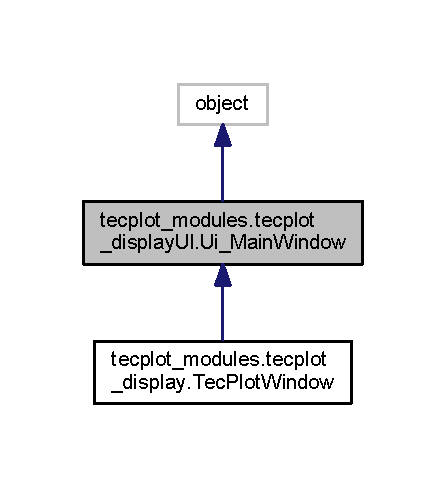
\includegraphics[width=214pt]{classtecplot__modules_1_1tecplot__display_u_i_1_1_ui___main_window__inherit__graph}
\end{center}
\end{figure}
\subsection*{Public Member Functions}
\begin{DoxyCompactItemize}
\item 
def \hyperlink{classtecplot__modules_1_1tecplot__display_u_i_1_1_ui___main_window_a84d83568b72995fc1f091c00044adb72}{setup\+Ui} (self, \hyperlink{namespacetecplot__modules_1_1tecplot__display_u_i_a05b56eca3c779fabf41fa975030e6ca1}{Main\+Window})
\item 
def \hyperlink{classtecplot__modules_1_1tecplot__display_u_i_1_1_ui___main_window_ae1811975426f7bbfcbe9bd6ae8a4d444}{retranslate\+Ui} (self, \hyperlink{namespacetecplot__modules_1_1tecplot__display_u_i_a05b56eca3c779fabf41fa975030e6ca1}{Main\+Window})
\end{DoxyCompactItemize}
\subsection*{Public Attributes}
\begin{DoxyCompactItemize}
\item 
\hyperlink{classtecplot__modules_1_1tecplot__display_u_i_1_1_ui___main_window_a8806355d8f5b1e79e73c21d82b2a02b1}{centralwidget}
\item 
\hyperlink{classtecplot__modules_1_1tecplot__display_u_i_1_1_ui___main_window_a5bc16af243ddcb715ac4dca3eaeea83f}{ui\+\_\+tecplot1\+\_\+dockw}
\item 
\hyperlink{classtecplot__modules_1_1tecplot__display_u_i_1_1_ui___main_window_a5f2617d5cf96b7f5c5eab71716630e9f}{dock\+Widget\+Contents}
\item 
\hyperlink{classtecplot__modules_1_1tecplot__display_u_i_1_1_ui___main_window_a669ef5be286de5a4683863273aea2117}{ui\+\_\+tecplot1\+\_\+dockcontents\+\_\+vl}
\item 
\hyperlink{classtecplot__modules_1_1tecplot__display_u_i_1_1_ui___main_window_a0e12cc099f3392ddc5763b2e11735c65}{ui\+\_\+tecplot1\+\_\+widget}
\item 
\hyperlink{classtecplot__modules_1_1tecplot__display_u_i_1_1_ui___main_window_a29ec621d9a4d64b9ac2741603bfd4c0b}{ui\+\_\+tecplot1\+\_\+widget\+\_\+vl}
\item 
\hyperlink{classtecplot__modules_1_1tecplot__display_u_i_1_1_ui___main_window_a39ab796d26cd8af1d7b08a1af13f18d3}{ui\+\_\+tecplot2\+\_\+dockw}
\item 
\hyperlink{classtecplot__modules_1_1tecplot__display_u_i_1_1_ui___main_window_afcc75b6eb098b33d244b16c759c2b0fd}{ui\+\_\+tecplot2\+\_\+dockcontents}
\item 
\hyperlink{classtecplot__modules_1_1tecplot__display_u_i_1_1_ui___main_window_a8883278a682ade2e54c270ba2064a3d8}{ui\+\_\+tecplot2\+\_\+dockcontents\+\_\+vl}
\item 
\hyperlink{classtecplot__modules_1_1tecplot__display_u_i_1_1_ui___main_window_adf880d85360d7fc4761f74c7ab80e09f}{ui\+\_\+tecplot\+\_\+widget\+\_\+2}
\item 
\hyperlink{classtecplot__modules_1_1tecplot__display_u_i_1_1_ui___main_window_a3b0bcb24fdafc82b684e59b018c76ba9}{ui\+\_\+tecplot2\+\_\+widget\+\_\+vl}
\end{DoxyCompactItemize}


\subsection{Member Function Documentation}
\hypertarget{classtecplot__modules_1_1tecplot__display_u_i_1_1_ui___main_window_ae1811975426f7bbfcbe9bd6ae8a4d444}{}\label{classtecplot__modules_1_1tecplot__display_u_i_1_1_ui___main_window_ae1811975426f7bbfcbe9bd6ae8a4d444} 
\index{tecplot\+\_\+modules\+::tecplot\+\_\+display\+U\+I\+::\+Ui\+\_\+\+Main\+Window@{tecplot\+\_\+modules\+::tecplot\+\_\+display\+U\+I\+::\+Ui\+\_\+\+Main\+Window}!retranslate\+Ui@{retranslate\+Ui}}
\index{retranslate\+Ui@{retranslate\+Ui}!tecplot\+\_\+modules\+::tecplot\+\_\+display\+U\+I\+::\+Ui\+\_\+\+Main\+Window@{tecplot\+\_\+modules\+::tecplot\+\_\+display\+U\+I\+::\+Ui\+\_\+\+Main\+Window}}
\subsubsection{\texorpdfstring{retranslate\+Ui()}{retranslateUi()}}
{\footnotesize\ttfamily def tecplot\+\_\+modules.\+tecplot\+\_\+display\+U\+I.\+Ui\+\_\+\+Main\+Window.\+retranslate\+Ui (\begin{DoxyParamCaption}\item[{}]{self,  }\item[{}]{Main\+Window }\end{DoxyParamCaption})}

\hypertarget{classtecplot__modules_1_1tecplot__display_u_i_1_1_ui___main_window_a84d83568b72995fc1f091c00044adb72}{}\label{classtecplot__modules_1_1tecplot__display_u_i_1_1_ui___main_window_a84d83568b72995fc1f091c00044adb72} 
\index{tecplot\+\_\+modules\+::tecplot\+\_\+display\+U\+I\+::\+Ui\+\_\+\+Main\+Window@{tecplot\+\_\+modules\+::tecplot\+\_\+display\+U\+I\+::\+Ui\+\_\+\+Main\+Window}!setup\+Ui@{setup\+Ui}}
\index{setup\+Ui@{setup\+Ui}!tecplot\+\_\+modules\+::tecplot\+\_\+display\+U\+I\+::\+Ui\+\_\+\+Main\+Window@{tecplot\+\_\+modules\+::tecplot\+\_\+display\+U\+I\+::\+Ui\+\_\+\+Main\+Window}}
\subsubsection{\texorpdfstring{setup\+Ui()}{setupUi()}}
{\footnotesize\ttfamily def tecplot\+\_\+modules.\+tecplot\+\_\+display\+U\+I.\+Ui\+\_\+\+Main\+Window.\+setup\+Ui (\begin{DoxyParamCaption}\item[{}]{self,  }\item[{}]{Main\+Window }\end{DoxyParamCaption})}



\subsection{Member Data Documentation}
\hypertarget{classtecplot__modules_1_1tecplot__display_u_i_1_1_ui___main_window_a8806355d8f5b1e79e73c21d82b2a02b1}{}\label{classtecplot__modules_1_1tecplot__display_u_i_1_1_ui___main_window_a8806355d8f5b1e79e73c21d82b2a02b1} 
\index{tecplot\+\_\+modules\+::tecplot\+\_\+display\+U\+I\+::\+Ui\+\_\+\+Main\+Window@{tecplot\+\_\+modules\+::tecplot\+\_\+display\+U\+I\+::\+Ui\+\_\+\+Main\+Window}!centralwidget@{centralwidget}}
\index{centralwidget@{centralwidget}!tecplot\+\_\+modules\+::tecplot\+\_\+display\+U\+I\+::\+Ui\+\_\+\+Main\+Window@{tecplot\+\_\+modules\+::tecplot\+\_\+display\+U\+I\+::\+Ui\+\_\+\+Main\+Window}}
\subsubsection{\texorpdfstring{centralwidget}{centralwidget}}
{\footnotesize\ttfamily tecplot\+\_\+modules.\+tecplot\+\_\+display\+U\+I.\+Ui\+\_\+\+Main\+Window.\+centralwidget}

\hypertarget{classtecplot__modules_1_1tecplot__display_u_i_1_1_ui___main_window_a5f2617d5cf96b7f5c5eab71716630e9f}{}\label{classtecplot__modules_1_1tecplot__display_u_i_1_1_ui___main_window_a5f2617d5cf96b7f5c5eab71716630e9f} 
\index{tecplot\+\_\+modules\+::tecplot\+\_\+display\+U\+I\+::\+Ui\+\_\+\+Main\+Window@{tecplot\+\_\+modules\+::tecplot\+\_\+display\+U\+I\+::\+Ui\+\_\+\+Main\+Window}!dock\+Widget\+Contents@{dock\+Widget\+Contents}}
\index{dock\+Widget\+Contents@{dock\+Widget\+Contents}!tecplot\+\_\+modules\+::tecplot\+\_\+display\+U\+I\+::\+Ui\+\_\+\+Main\+Window@{tecplot\+\_\+modules\+::tecplot\+\_\+display\+U\+I\+::\+Ui\+\_\+\+Main\+Window}}
\subsubsection{\texorpdfstring{dock\+Widget\+Contents}{dockWidgetContents}}
{\footnotesize\ttfamily tecplot\+\_\+modules.\+tecplot\+\_\+display\+U\+I.\+Ui\+\_\+\+Main\+Window.\+dock\+Widget\+Contents}

\hypertarget{classtecplot__modules_1_1tecplot__display_u_i_1_1_ui___main_window_a669ef5be286de5a4683863273aea2117}{}\label{classtecplot__modules_1_1tecplot__display_u_i_1_1_ui___main_window_a669ef5be286de5a4683863273aea2117} 
\index{tecplot\+\_\+modules\+::tecplot\+\_\+display\+U\+I\+::\+Ui\+\_\+\+Main\+Window@{tecplot\+\_\+modules\+::tecplot\+\_\+display\+U\+I\+::\+Ui\+\_\+\+Main\+Window}!ui\+\_\+tecplot1\+\_\+dockcontents\+\_\+vl@{ui\+\_\+tecplot1\+\_\+dockcontents\+\_\+vl}}
\index{ui\+\_\+tecplot1\+\_\+dockcontents\+\_\+vl@{ui\+\_\+tecplot1\+\_\+dockcontents\+\_\+vl}!tecplot\+\_\+modules\+::tecplot\+\_\+display\+U\+I\+::\+Ui\+\_\+\+Main\+Window@{tecplot\+\_\+modules\+::tecplot\+\_\+display\+U\+I\+::\+Ui\+\_\+\+Main\+Window}}
\subsubsection{\texorpdfstring{ui\+\_\+tecplot1\+\_\+dockcontents\+\_\+vl}{ui\_tecplot1\_dockcontents\_vl}}
{\footnotesize\ttfamily tecplot\+\_\+modules.\+tecplot\+\_\+display\+U\+I.\+Ui\+\_\+\+Main\+Window.\+ui\+\_\+tecplot1\+\_\+dockcontents\+\_\+vl}

\hypertarget{classtecplot__modules_1_1tecplot__display_u_i_1_1_ui___main_window_a5bc16af243ddcb715ac4dca3eaeea83f}{}\label{classtecplot__modules_1_1tecplot__display_u_i_1_1_ui___main_window_a5bc16af243ddcb715ac4dca3eaeea83f} 
\index{tecplot\+\_\+modules\+::tecplot\+\_\+display\+U\+I\+::\+Ui\+\_\+\+Main\+Window@{tecplot\+\_\+modules\+::tecplot\+\_\+display\+U\+I\+::\+Ui\+\_\+\+Main\+Window}!ui\+\_\+tecplot1\+\_\+dockw@{ui\+\_\+tecplot1\+\_\+dockw}}
\index{ui\+\_\+tecplot1\+\_\+dockw@{ui\+\_\+tecplot1\+\_\+dockw}!tecplot\+\_\+modules\+::tecplot\+\_\+display\+U\+I\+::\+Ui\+\_\+\+Main\+Window@{tecplot\+\_\+modules\+::tecplot\+\_\+display\+U\+I\+::\+Ui\+\_\+\+Main\+Window}}
\subsubsection{\texorpdfstring{ui\+\_\+tecplot1\+\_\+dockw}{ui\_tecplot1\_dockw}}
{\footnotesize\ttfamily tecplot\+\_\+modules.\+tecplot\+\_\+display\+U\+I.\+Ui\+\_\+\+Main\+Window.\+ui\+\_\+tecplot1\+\_\+dockw}

\hypertarget{classtecplot__modules_1_1tecplot__display_u_i_1_1_ui___main_window_a0e12cc099f3392ddc5763b2e11735c65}{}\label{classtecplot__modules_1_1tecplot__display_u_i_1_1_ui___main_window_a0e12cc099f3392ddc5763b2e11735c65} 
\index{tecplot\+\_\+modules\+::tecplot\+\_\+display\+U\+I\+::\+Ui\+\_\+\+Main\+Window@{tecplot\+\_\+modules\+::tecplot\+\_\+display\+U\+I\+::\+Ui\+\_\+\+Main\+Window}!ui\+\_\+tecplot1\+\_\+widget@{ui\+\_\+tecplot1\+\_\+widget}}
\index{ui\+\_\+tecplot1\+\_\+widget@{ui\+\_\+tecplot1\+\_\+widget}!tecplot\+\_\+modules\+::tecplot\+\_\+display\+U\+I\+::\+Ui\+\_\+\+Main\+Window@{tecplot\+\_\+modules\+::tecplot\+\_\+display\+U\+I\+::\+Ui\+\_\+\+Main\+Window}}
\subsubsection{\texorpdfstring{ui\+\_\+tecplot1\+\_\+widget}{ui\_tecplot1\_widget}}
{\footnotesize\ttfamily tecplot\+\_\+modules.\+tecplot\+\_\+display\+U\+I.\+Ui\+\_\+\+Main\+Window.\+ui\+\_\+tecplot1\+\_\+widget}

\hypertarget{classtecplot__modules_1_1tecplot__display_u_i_1_1_ui___main_window_a29ec621d9a4d64b9ac2741603bfd4c0b}{}\label{classtecplot__modules_1_1tecplot__display_u_i_1_1_ui___main_window_a29ec621d9a4d64b9ac2741603bfd4c0b} 
\index{tecplot\+\_\+modules\+::tecplot\+\_\+display\+U\+I\+::\+Ui\+\_\+\+Main\+Window@{tecplot\+\_\+modules\+::tecplot\+\_\+display\+U\+I\+::\+Ui\+\_\+\+Main\+Window}!ui\+\_\+tecplot1\+\_\+widget\+\_\+vl@{ui\+\_\+tecplot1\+\_\+widget\+\_\+vl}}
\index{ui\+\_\+tecplot1\+\_\+widget\+\_\+vl@{ui\+\_\+tecplot1\+\_\+widget\+\_\+vl}!tecplot\+\_\+modules\+::tecplot\+\_\+display\+U\+I\+::\+Ui\+\_\+\+Main\+Window@{tecplot\+\_\+modules\+::tecplot\+\_\+display\+U\+I\+::\+Ui\+\_\+\+Main\+Window}}
\subsubsection{\texorpdfstring{ui\+\_\+tecplot1\+\_\+widget\+\_\+vl}{ui\_tecplot1\_widget\_vl}}
{\footnotesize\ttfamily tecplot\+\_\+modules.\+tecplot\+\_\+display\+U\+I.\+Ui\+\_\+\+Main\+Window.\+ui\+\_\+tecplot1\+\_\+widget\+\_\+vl}

\hypertarget{classtecplot__modules_1_1tecplot__display_u_i_1_1_ui___main_window_afcc75b6eb098b33d244b16c759c2b0fd}{}\label{classtecplot__modules_1_1tecplot__display_u_i_1_1_ui___main_window_afcc75b6eb098b33d244b16c759c2b0fd} 
\index{tecplot\+\_\+modules\+::tecplot\+\_\+display\+U\+I\+::\+Ui\+\_\+\+Main\+Window@{tecplot\+\_\+modules\+::tecplot\+\_\+display\+U\+I\+::\+Ui\+\_\+\+Main\+Window}!ui\+\_\+tecplot2\+\_\+dockcontents@{ui\+\_\+tecplot2\+\_\+dockcontents}}
\index{ui\+\_\+tecplot2\+\_\+dockcontents@{ui\+\_\+tecplot2\+\_\+dockcontents}!tecplot\+\_\+modules\+::tecplot\+\_\+display\+U\+I\+::\+Ui\+\_\+\+Main\+Window@{tecplot\+\_\+modules\+::tecplot\+\_\+display\+U\+I\+::\+Ui\+\_\+\+Main\+Window}}
\subsubsection{\texorpdfstring{ui\+\_\+tecplot2\+\_\+dockcontents}{ui\_tecplot2\_dockcontents}}
{\footnotesize\ttfamily tecplot\+\_\+modules.\+tecplot\+\_\+display\+U\+I.\+Ui\+\_\+\+Main\+Window.\+ui\+\_\+tecplot2\+\_\+dockcontents}

\hypertarget{classtecplot__modules_1_1tecplot__display_u_i_1_1_ui___main_window_a8883278a682ade2e54c270ba2064a3d8}{}\label{classtecplot__modules_1_1tecplot__display_u_i_1_1_ui___main_window_a8883278a682ade2e54c270ba2064a3d8} 
\index{tecplot\+\_\+modules\+::tecplot\+\_\+display\+U\+I\+::\+Ui\+\_\+\+Main\+Window@{tecplot\+\_\+modules\+::tecplot\+\_\+display\+U\+I\+::\+Ui\+\_\+\+Main\+Window}!ui\+\_\+tecplot2\+\_\+dockcontents\+\_\+vl@{ui\+\_\+tecplot2\+\_\+dockcontents\+\_\+vl}}
\index{ui\+\_\+tecplot2\+\_\+dockcontents\+\_\+vl@{ui\+\_\+tecplot2\+\_\+dockcontents\+\_\+vl}!tecplot\+\_\+modules\+::tecplot\+\_\+display\+U\+I\+::\+Ui\+\_\+\+Main\+Window@{tecplot\+\_\+modules\+::tecplot\+\_\+display\+U\+I\+::\+Ui\+\_\+\+Main\+Window}}
\subsubsection{\texorpdfstring{ui\+\_\+tecplot2\+\_\+dockcontents\+\_\+vl}{ui\_tecplot2\_dockcontents\_vl}}
{\footnotesize\ttfamily tecplot\+\_\+modules.\+tecplot\+\_\+display\+U\+I.\+Ui\+\_\+\+Main\+Window.\+ui\+\_\+tecplot2\+\_\+dockcontents\+\_\+vl}

\hypertarget{classtecplot__modules_1_1tecplot__display_u_i_1_1_ui___main_window_a39ab796d26cd8af1d7b08a1af13f18d3}{}\label{classtecplot__modules_1_1tecplot__display_u_i_1_1_ui___main_window_a39ab796d26cd8af1d7b08a1af13f18d3} 
\index{tecplot\+\_\+modules\+::tecplot\+\_\+display\+U\+I\+::\+Ui\+\_\+\+Main\+Window@{tecplot\+\_\+modules\+::tecplot\+\_\+display\+U\+I\+::\+Ui\+\_\+\+Main\+Window}!ui\+\_\+tecplot2\+\_\+dockw@{ui\+\_\+tecplot2\+\_\+dockw}}
\index{ui\+\_\+tecplot2\+\_\+dockw@{ui\+\_\+tecplot2\+\_\+dockw}!tecplot\+\_\+modules\+::tecplot\+\_\+display\+U\+I\+::\+Ui\+\_\+\+Main\+Window@{tecplot\+\_\+modules\+::tecplot\+\_\+display\+U\+I\+::\+Ui\+\_\+\+Main\+Window}}
\subsubsection{\texorpdfstring{ui\+\_\+tecplot2\+\_\+dockw}{ui\_tecplot2\_dockw}}
{\footnotesize\ttfamily tecplot\+\_\+modules.\+tecplot\+\_\+display\+U\+I.\+Ui\+\_\+\+Main\+Window.\+ui\+\_\+tecplot2\+\_\+dockw}

\hypertarget{classtecplot__modules_1_1tecplot__display_u_i_1_1_ui___main_window_a3b0bcb24fdafc82b684e59b018c76ba9}{}\label{classtecplot__modules_1_1tecplot__display_u_i_1_1_ui___main_window_a3b0bcb24fdafc82b684e59b018c76ba9} 
\index{tecplot\+\_\+modules\+::tecplot\+\_\+display\+U\+I\+::\+Ui\+\_\+\+Main\+Window@{tecplot\+\_\+modules\+::tecplot\+\_\+display\+U\+I\+::\+Ui\+\_\+\+Main\+Window}!ui\+\_\+tecplot2\+\_\+widget\+\_\+vl@{ui\+\_\+tecplot2\+\_\+widget\+\_\+vl}}
\index{ui\+\_\+tecplot2\+\_\+widget\+\_\+vl@{ui\+\_\+tecplot2\+\_\+widget\+\_\+vl}!tecplot\+\_\+modules\+::tecplot\+\_\+display\+U\+I\+::\+Ui\+\_\+\+Main\+Window@{tecplot\+\_\+modules\+::tecplot\+\_\+display\+U\+I\+::\+Ui\+\_\+\+Main\+Window}}
\subsubsection{\texorpdfstring{ui\+\_\+tecplot2\+\_\+widget\+\_\+vl}{ui\_tecplot2\_widget\_vl}}
{\footnotesize\ttfamily tecplot\+\_\+modules.\+tecplot\+\_\+display\+U\+I.\+Ui\+\_\+\+Main\+Window.\+ui\+\_\+tecplot2\+\_\+widget\+\_\+vl}

\hypertarget{classtecplot__modules_1_1tecplot__display_u_i_1_1_ui___main_window_adf880d85360d7fc4761f74c7ab80e09f}{}\label{classtecplot__modules_1_1tecplot__display_u_i_1_1_ui___main_window_adf880d85360d7fc4761f74c7ab80e09f} 
\index{tecplot\+\_\+modules\+::tecplot\+\_\+display\+U\+I\+::\+Ui\+\_\+\+Main\+Window@{tecplot\+\_\+modules\+::tecplot\+\_\+display\+U\+I\+::\+Ui\+\_\+\+Main\+Window}!ui\+\_\+tecplot\+\_\+widget\+\_\+2@{ui\+\_\+tecplot\+\_\+widget\+\_\+2}}
\index{ui\+\_\+tecplot\+\_\+widget\+\_\+2@{ui\+\_\+tecplot\+\_\+widget\+\_\+2}!tecplot\+\_\+modules\+::tecplot\+\_\+display\+U\+I\+::\+Ui\+\_\+\+Main\+Window@{tecplot\+\_\+modules\+::tecplot\+\_\+display\+U\+I\+::\+Ui\+\_\+\+Main\+Window}}
\subsubsection{\texorpdfstring{ui\+\_\+tecplot\+\_\+widget\+\_\+2}{ui\_tecplot\_widget\_2}}
{\footnotesize\ttfamily tecplot\+\_\+modules.\+tecplot\+\_\+display\+U\+I.\+Ui\+\_\+\+Main\+Window.\+ui\+\_\+tecplot\+\_\+widget\+\_\+2}



The documentation for this class was generated from the following file\+:\begin{DoxyCompactItemize}
\item 
\hyperlink{tecplot__modules_2tecplot__display_u_i_8py}{tecplot\+\_\+modules/tecplot\+\_\+display\+U\+I.\+py}\end{DoxyCompactItemize}

\hypertarget{classbladepro__modules_1_1inputfile__writer_u_i_1_1_ui___main_window}{}\section{bladepro\+\_\+modules.\+inputfile\+\_\+writer\+U\+I.\+Ui\+\_\+\+Main\+Window Class Reference}
\label{classbladepro__modules_1_1inputfile__writer_u_i_1_1_ui___main_window}\index{bladepro\+\_\+modules.\+inputfile\+\_\+writer\+U\+I.\+Ui\+\_\+\+Main\+Window@{bladepro\+\_\+modules.\+inputfile\+\_\+writer\+U\+I.\+Ui\+\_\+\+Main\+Window}}


Inheritance diagram for bladepro\+\_\+modules.\+inputfile\+\_\+writer\+U\+I.\+Ui\+\_\+\+Main\+Window\+:\nopagebreak
\begin{figure}[H]
\begin{center}
\leavevmode
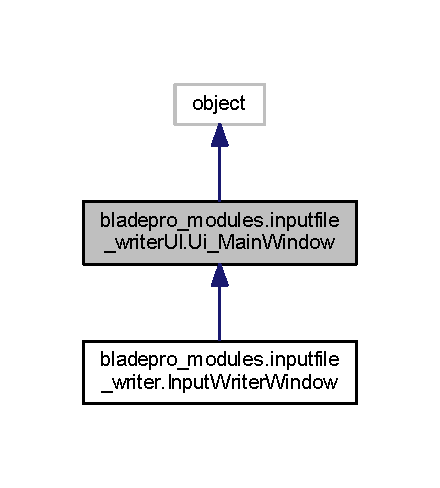
\includegraphics[width=211pt]{classbladepro__modules_1_1inputfile__writer_u_i_1_1_ui___main_window__inherit__graph}
\end{center}
\end{figure}
\subsection*{Public Member Functions}
\begin{DoxyCompactItemize}
\item 
def \hyperlink{classbladepro__modules_1_1inputfile__writer_u_i_1_1_ui___main_window_a77688f6f653ba2711e93269a03753754}{setup\+Ui} (self, \hyperlink{namespacebladepro__modules_1_1inputfile__writer_u_i_ab649489a40967421c06970ba9ffeef53}{Main\+Window})
\item 
def \hyperlink{classbladepro__modules_1_1inputfile__writer_u_i_1_1_ui___main_window_a640f34d5228b66fcf4118eaa17edf8d6}{retranslate\+Ui} (self, \hyperlink{namespacebladepro__modules_1_1inputfile__writer_u_i_ab649489a40967421c06970ba9ffeef53}{Main\+Window})
\end{DoxyCompactItemize}
\subsection*{Public Attributes}
\begin{DoxyCompactItemize}
\item 
\hyperlink{classbladepro__modules_1_1inputfile__writer_u_i_1_1_ui___main_window_a99bcc614e5be2356b9b0e54f30bb009e}{centralwidget}
\item 
\hyperlink{classbladepro__modules_1_1inputfile__writer_u_i_1_1_ui___main_window_aad085c53319e511b5f37895a71336716}{grid\+Layout}
\item 
\hyperlink{classbladepro__modules_1_1inputfile__writer_u_i_1_1_ui___main_window_a342c5c54417df97a32a10f28fe93d81e}{ui\+\_\+output\+\_\+groupbox}
\item 
\hyperlink{classbladepro__modules_1_1inputfile__writer_u_i_1_1_ui___main_window_ae33ea0222b6e62c39a7081946f32072a}{vertical\+Layout}
\item 
\hyperlink{classbladepro__modules_1_1inputfile__writer_u_i_1_1_ui___main_window_ad528f27c7c549b388b9a6dc2e24f9880}{grid\+Layout\+\_\+3}
\item 
\hyperlink{classbladepro__modules_1_1inputfile__writer_u_i_1_1_ui___main_window_a55227446d0a73588ace14f77945ec2ee}{line\+\_\+6}
\item 
\hyperlink{classbladepro__modules_1_1inputfile__writer_u_i_1_1_ui___main_window_a8020c73e1cf12f6c112a79f2c34af062}{ui\+\_\+output\+\_\+mappnts\+\_\+pointsfile\+\_\+edit}
\item 
\hyperlink{classbladepro__modules_1_1inputfile__writer_u_i_1_1_ui___main_window_a47635280e1268bda03a8e1f69a03fc35}{ui\+\_\+output\+\_\+tecplot\+\_\+3d\+\_\+chk}
\item 
\hyperlink{classbladepro__modules_1_1inputfile__writer_u_i_1_1_ui___main_window_a08c1ff077d7bec4a77e7f540b681c71a}{ui\+\_\+output\+\_\+tecplot\+\_\+streams\+\_\+chk}
\item 
\hyperlink{classbladepro__modules_1_1inputfile__writer_u_i_1_1_ui___main_window_a7689384c6c651ee544d44f0029a731b5}{ui\+\_\+output\+\_\+cft\+\_\+nsect\+\_\+spn}
\item 
\hyperlink{classbladepro__modules_1_1inputfile__writer_u_i_1_1_ui___main_window_a7376266aa4a7bdb95b74e14c4e2294c0}{ui\+\_\+output\+\_\+streamc\+\_\+npoints\+\_\+spn}
\item 
\hyperlink{classbladepro__modules_1_1inputfile__writer_u_i_1_1_ui___main_window_a51d1efb48954a11443baee2265fb4a2a}{ui\+\_\+output\+\_\+stackcur\+\_\+stackpos\+\_\+dspn}
\item 
\hyperlink{classbladepro__modules_1_1inputfile__writer_u_i_1_1_ui___main_window_ac1c6cd8619b834a5b653a36f784fb43e}{ui\+\_\+output\+\_\+sweepangle\+\_\+lbl}
\item 
\hyperlink{classbladepro__modules_1_1inputfile__writer_u_i_1_1_ui___main_window_aacdb4037b930e2ee45ab5c333990a969}{ui\+\_\+output\+\_\+tecplot\+\_\+3d\+\_\+lbl}
\item 
\hyperlink{classbladepro__modules_1_1inputfile__writer_u_i_1_1_ui___main_window_aa8b180aa3d27924eb0fe24e40d2bb03e}{ui\+\_\+output\+\_\+autogrid\+\_\+lbl}
\item 
\hyperlink{classbladepro__modules_1_1inputfile__writer_u_i_1_1_ui___main_window_ad31bb569d28370ccbd2b76bb7a4b8b89}{ui\+\_\+output\+\_\+autogrid\+\_\+chk}
\item 
\hyperlink{classbladepro__modules_1_1inputfile__writer_u_i_1_1_ui___main_window_a726af21c576e9cfa777b00fa72b6eadf}{ui\+\_\+output\+\_\+rtzt\+\_\+npoints\+\_\+spn}
\item 
\hyperlink{classbladepro__modules_1_1inputfile__writer_u_i_1_1_ui___main_window_ad6ef09a5ac4e379fd644cd77d0db11ca}{ui\+\_\+output\+\_\+tecplot\+\_\+streams\+\_\+lbl}
\item 
\hyperlink{classbladepro__modules_1_1inputfile__writer_u_i_1_1_ui___main_window_af13e62fd96ef8e9fd80f03ca365f9117}{ui\+\_\+output\+\_\+sweepangle\+\_\+chk}
\item 
\hyperlink{classbladepro__modules_1_1inputfile__writer_u_i_1_1_ui___main_window_a8b6a216e0c5079501ecb0faf10f28a9b}{ui\+\_\+output\+\_\+heighv\+\_\+lbl}
\item 
\hyperlink{classbladepro__modules_1_1inputfile__writer_u_i_1_1_ui___main_window_a7164809ee0f9eaf1fc8ef281866630e6}{line\+\_\+4}
\item 
\hyperlink{classbladepro__modules_1_1inputfile__writer_u_i_1_1_ui___main_window_af03231f676dd6187432bb4007a3056dd}{line\+\_\+8}
\item 
\hyperlink{classbladepro__modules_1_1inputfile__writer_u_i_1_1_ui___main_window_ad08c484a4323a6f6051cf71cfa1a208e}{line\+\_\+3}
\item 
\hyperlink{classbladepro__modules_1_1inputfile__writer_u_i_1_1_ui___main_window_a72d1aa573f44078c64d2e5c063ef15ba}{ui\+\_\+output\+\_\+heighv\+\_\+chk}
\item 
\hyperlink{classbladepro__modules_1_1inputfile__writer_u_i_1_1_ui___main_window_a3a0f0c6441ea06c8a04d5dc13cb2dc8e}{ui\+\_\+output\+\_\+streamc\+\_\+chk}
\item 
\hyperlink{classbladepro__modules_1_1inputfile__writer_u_i_1_1_ui___main_window_a1436e56fad76cd38cf1f87db08b539b8}{ui\+\_\+output\+\_\+streamc\+\_\+lbl}
\item 
\hyperlink{classbladepro__modules_1_1inputfile__writer_u_i_1_1_ui___main_window_a336846c91ac57b8ab8ab0f2b5c5a0b9e}{ui\+\_\+output\+\_\+rtzt\+\_\+chk}
\item 
\hyperlink{classbladepro__modules_1_1inputfile__writer_u_i_1_1_ui___main_window_a806b947963fcab17402d6c5b4cc16368}{ui\+\_\+output\+\_\+mappnts\+\_\+streamcurvefile\+\_\+edit}
\item 
\hyperlink{classbladepro__modules_1_1inputfile__writer_u_i_1_1_ui___main_window_a17ad2111dee7da23381837dc87ce9a6c}{ui\+\_\+output\+\_\+rtzt\+\_\+lbl}
\item 
\hyperlink{classbladepro__modules_1_1inputfile__writer_u_i_1_1_ui___main_window_a1b032189cdd7d3d01263d73bfd778d92}{ui\+\_\+output\+\_\+cft\+\_\+chk}
\item 
\hyperlink{classbladepro__modules_1_1inputfile__writer_u_i_1_1_ui___main_window_ae4dbdbe6b6da83089c1ae51bb6cdb1e2}{ui\+\_\+output\+\_\+streamc\+\_\+extension\+\_\+dspn}
\item 
\hyperlink{classbladepro__modules_1_1inputfile__writer_u_i_1_1_ui___main_window_ac2158a8a751f8d5478c20a551799d3b1}{ui\+\_\+output\+\_\+cft\+\_\+lbl}
\item 
\hyperlink{classbladepro__modules_1_1inputfile__writer_u_i_1_1_ui___main_window_afcb54ff967d6a7fc001c9714f038ab80}{ui\+\_\+output\+\_\+mappnts\+\_\+chk}
\item 
\hyperlink{classbladepro__modules_1_1inputfile__writer_u_i_1_1_ui___main_window_a96c4756f82fdfe6fa5385898c3d96a91}{ui\+\_\+output\+\_\+mappnts\+\_\+lbl}
\item 
\hyperlink{classbladepro__modules_1_1inputfile__writer_u_i_1_1_ui___main_window_a9a81933c3dedf38f28446661eb6796fa}{ui\+\_\+output\+\_\+stackcur\+\_\+opt\+\_\+combo}
\item 
\hyperlink{classbladepro__modules_1_1inputfile__writer_u_i_1_1_ui___main_window_af92fe733419818e322c45b716966440b}{ui\+\_\+output\+\_\+heighv\+\_\+hvar\+\_\+spn}
\item 
\hyperlink{classbladepro__modules_1_1inputfile__writer_u_i_1_1_ui___main_window_aa8751b98f2848d66d991f668a8061b50}{ui\+\_\+output\+\_\+cft\+\_\+angle\+\_\+dspn}
\item 
\hyperlink{classbladepro__modules_1_1inputfile__writer_u_i_1_1_ui___main_window_a0ce457bc120667aadadd3ade828c65b3}{ui\+\_\+output\+\_\+rtzt\+\_\+thickness\+\_\+dpsn}
\item 
\hyperlink{classbladepro__modules_1_1inputfile__writer_u_i_1_1_ui___main_window_a60d8702dcef7ca077c25402d981a2ba9}{ui\+\_\+output\+\_\+stackcur\+\_\+chk}
\item 
\hyperlink{classbladepro__modules_1_1inputfile__writer_u_i_1_1_ui___main_window_abd1aece55a53a090e79fd1a7449d67b8}{ui\+\_\+output\+\_\+stackcur\+\_\+lbl}
\item 
\hyperlink{classbladepro__modules_1_1inputfile__writer_u_i_1_1_ui___main_window_a02aad1387d04c6ec5ad12e80a6a59d08}{ui\+\_\+output\+\_\+igs\+\_\+pnts2pnts\+\_\+chk}
\item 
\hyperlink{classbladepro__modules_1_1inputfile__writer_u_i_1_1_ui___main_window_a9a3e7b7353a08d8254630806f3466fc3}{ui\+\_\+output\+\_\+igs\+\_\+pnts2cur\+\_\+lbl\+\_\+2}
\item 
\hyperlink{classbladepro__modules_1_1inputfile__writer_u_i_1_1_ui___main_window_a3a6ca0d33559a544c30ca69a584f5fb3}{ui\+\_\+output\+\_\+igs\+\_\+pnts2cur\+\_\+lbl}
\item 
\hyperlink{classbladepro__modules_1_1inputfile__writer_u_i_1_1_ui___main_window_acdf536fc7b4d652bfde2a129ac63af81}{ui\+\_\+output\+\_\+igs\+\_\+pnts2pnts\+\_\+file\+\_\+edit}
\item 
\hyperlink{classbladepro__modules_1_1inputfile__writer_u_i_1_1_ui___main_window_a47f948d0d305ed25b5d4199199348306}{ui\+\_\+output\+\_\+lecur\+\_\+lbl}
\item 
\hyperlink{classbladepro__modules_1_1inputfile__writer_u_i_1_1_ui___main_window_af26afcf143419489f7a9c388f242550b}{ui\+\_\+output\+\_\+lecur\+\_\+chk}
\item 
\hyperlink{classbladepro__modules_1_1inputfile__writer_u_i_1_1_ui___main_window_afccfcfd87634348612a93710d25902d6}{ui\+\_\+output\+\_\+lecur\+\_\+npoints\+\_\+spn}
\item 
\hyperlink{classbladepro__modules_1_1inputfile__writer_u_i_1_1_ui___main_window_a9b081326a67dee3b6ab18d2aa0937b1a}{line\+\_\+10}
\item 
\hyperlink{classbladepro__modules_1_1inputfile__writer_u_i_1_1_ui___main_window_a550f0dbb76e9a3094c1e38b46f5d885d}{ui\+\_\+output\+\_\+igs\+\_\+pnts2cur\+\_\+chk}
\item 
\hyperlink{classbladepro__modules_1_1inputfile__writer_u_i_1_1_ui___main_window_a1fd1e46b01841149ab493b773c6ee08c}{ui\+\_\+output\+\_\+tepos\+\_\+chk}
\item 
\hyperlink{classbladepro__modules_1_1inputfile__writer_u_i_1_1_ui___main_window_afc059e5843391ef3e3c56edb1f201cc0}{ui\+\_\+output\+\_\+igs\+\_\+pnts2cur\+\_\+file\+\_\+edit}
\item 
\hyperlink{classbladepro__modules_1_1inputfile__writer_u_i_1_1_ui___main_window_af6b3a50b9ed8b101a02f8cd2103add7a}{ui\+\_\+output\+\_\+tecur\+\_\+lbl}
\item 
\hyperlink{classbladepro__modules_1_1inputfile__writer_u_i_1_1_ui___main_window_a8a199146fc853fdada7f050f108a22a2}{ui\+\_\+output\+\_\+tecur\+\_\+chk}
\item 
\hyperlink{classbladepro__modules_1_1inputfile__writer_u_i_1_1_ui___main_window_aec9a2b9c0199fa892631d906b1296a13}{ui\+\_\+output\+\_\+tecur\+\_\+npoints\+\_\+spn}
\item 
\hyperlink{classbladepro__modules_1_1inputfile__writer_u_i_1_1_ui___main_window_a0906e6ac9dd29621615af0e54f1b2768}{ui\+\_\+output\+\_\+tepos\+\_\+lbl}
\item 
\hyperlink{classbladepro__modules_1_1inputfile__writer_u_i_1_1_ui___main_window_a6250f7ec5670033a6994818abf3d9b15}{ui\+\_\+output\+\_\+camberangles\+\_\+chk}
\item 
\hyperlink{classbladepro__modules_1_1inputfile__writer_u_i_1_1_ui___main_window_ae0b09533ea5d38dcba89c010fcdc7886}{ui\+\_\+output\+\_\+camberangles\+\_\+lbl}
\item 
\hyperlink{classbladepro__modules_1_1inputfile__writer_u_i_1_1_ui___main_window_a8c262e36d39977da647517cb97b7ab86}{ui\+\_\+output\+\_\+camberangles\+\_\+opt\+\_\+combo}
\item 
\hyperlink{classbladepro__modules_1_1inputfile__writer_u_i_1_1_ui___main_window_a868061df5f5e844caea1728de203129e}{ui\+\_\+selectusersettings\+\_\+groupbox}
\item 
\hyperlink{classbladepro__modules_1_1inputfile__writer_u_i_1_1_ui___main_window_a5a42530f0dd7f8e7c2da3074565220be}{ui\+\_\+selectusersettings\+\_\+groupbox\+\_\+gl}
\item 
\hyperlink{classbladepro__modules_1_1inputfile__writer_u_i_1_1_ui___main_window_aa064aa43c06b096e6d2753909fddf376}{ui\+\_\+user\+\_\+settings\+\_\+gl}
\item 
\hyperlink{classbladepro__modules_1_1inputfile__writer_u_i_1_1_ui___main_window_a1ac2324eaa26fdc7d7a038b7df328a0d}{ui\+\_\+listsettings\+\_\+combo}
\item 
\hyperlink{classbladepro__modules_1_1inputfile__writer_u_i_1_1_ui___main_window_a720608a6cc8575e078cd4e807dfe1031}{ui\+\_\+renamesetting\+\_\+btn}
\item 
\hyperlink{classbladepro__modules_1_1inputfile__writer_u_i_1_1_ui___main_window_af95ad0699234293c4dbeaa2fbf3af607}{ui\+\_\+quicklist\+\_\+chk}
\item 
\hyperlink{classbladepro__modules_1_1inputfile__writer_u_i_1_1_ui___main_window_afd5486e4e3b6a77faf883e45beab9a09}{ui\+\_\+read\+\_\+groupbox}
\item 
\hyperlink{classbladepro__modules_1_1inputfile__writer_u_i_1_1_ui___main_window_ad90bdfb90daa3db5b3f49ae0b8d8fa8e}{ui\+\_\+read\+\_\+groupbox\+\_\+gl}
\item 
\hyperlink{classbladepro__modules_1_1inputfile__writer_u_i_1_1_ui___main_window_a7704bdcb5a1c0e19f4cd1c19c2000b62}{ui\+\_\+read\+\_\+options\+\_\+gl}
\item 
\hyperlink{classbladepro__modules_1_1inputfile__writer_u_i_1_1_ui___main_window_a7bfc8ae9b8e66f044f312dbb91219d88}{ui\+\_\+read\+\_\+cftgeo\+\_\+angle\+\_\+dspn}
\item 
\hyperlink{classbladepro__modules_1_1inputfile__writer_u_i_1_1_ui___main_window_a96dfb7bb6ab5a36c649090a3d1178c74}{ui\+\_\+read\+\_\+cftgeo\+\_\+nblades\+\_\+spn}
\item 
\hyperlink{classbladepro__modules_1_1inputfile__writer_u_i_1_1_ui___main_window_a28522bd8330277ba8a1f01fa736cc82f}{ui\+\_\+read\+\_\+ibl\+\_\+iblfile\+\_\+edit}
\item 
\hyperlink{classbladepro__modules_1_1inputfile__writer_u_i_1_1_ui___main_window_a297dda79cc86d653c2ba1f5bdef3b70e}{ui\+\_\+read\+\_\+ibl\+\_\+lbl}
\item 
\hyperlink{classbladepro__modules_1_1inputfile__writer_u_i_1_1_ui___main_window_a5da571d939521a997ec7b05cd5bd7091}{ui\+\_\+read\+\_\+cftgeo\+\_\+cftfile\+\_\+edit}
\item 
\hyperlink{classbladepro__modules_1_1inputfile__writer_u_i_1_1_ui___main_window_abcf4d4a107f41021d2904f09770d747b}{ui\+\_\+read\+\_\+cftgeo\+\_\+lbl}
\item 
\hyperlink{classbladepro__modules_1_1inputfile__writer_u_i_1_1_ui___main_window_a94bf4df4cc948d1a55752fa45b97099b}{ui\+\_\+read\+\_\+ibl\+\_\+rbtn}
\item 
\hyperlink{classbladepro__modules_1_1inputfile__writer_u_i_1_1_ui___main_window_a3ccbf6ded4e6de7d70da7777441a3227}{ui\+\_\+read\+\_\+cftgeo\+\_\+rbtn}
\item 
\hyperlink{classbladepro__modules_1_1inputfile__writer_u_i_1_1_ui___main_window_a94ac3b9c86462bc353b5c9a53b961a7d}{ui\+\_\+read\+\_\+find\+\_\+btn}
\item 
\hyperlink{classbladepro__modules_1_1inputfile__writer_u_i_1_1_ui___main_window_a16200a07fd06dae2ce5c12674d04b497}{ui\+\_\+read\+\_\+ibl\+\_\+fpfile\+\_\+edit}
\item 
\hyperlink{classbladepro__modules_1_1inputfile__writer_u_i_1_1_ui___main_window_a050e1f0c2f0a5c8d15ca21021459c06d}{ui\+\_\+working\+\_\+case\+\_\+gl}
\item 
\hyperlink{classbladepro__modules_1_1inputfile__writer_u_i_1_1_ui___main_window_aae8ee2dceedfebed42a95b5122615de8}{ui\+\_\+working\+\_\+path\+\_\+lbl}
\item 
\hyperlink{classbladepro__modules_1_1inputfile__writer_u_i_1_1_ui___main_window_a0d4435462e6a1f2672c93af7e87b719c}{ui\+\_\+case\+\_\+name\+\_\+lbl}
\item 
\hyperlink{classbladepro__modules_1_1inputfile__writer_u_i_1_1_ui___main_window_ac790262e3ac621cfe957cdd36f94d817}{ui\+\_\+case\+\_\+name\+\_\+edit}
\item 
\hyperlink{classbladepro__modules_1_1inputfile__writer_u_i_1_1_ui___main_window_a7978ca560b83fbc4bd3859b7bba05153}{ui\+\_\+working\+\_\+path\+\_\+edit}
\item 
\hyperlink{classbladepro__modules_1_1inputfile__writer_u_i_1_1_ui___main_window_a007ebda4f46ac96952c59e60a2fa8f3b}{ui\+\_\+case\+\_\+name\+\_\+existent\+\_\+list}
\item 
\hyperlink{classbladepro__modules_1_1inputfile__writer_u_i_1_1_ui___main_window_a0f508ef0b3e47a027a63dd3cde363ef4}{ui\+\_\+select\+\_\+path\+\_\+btn}
\item 
\hyperlink{classbladepro__modules_1_1inputfile__writer_u_i_1_1_ui___main_window_adc08aa0dfe6e33f10acea28994425d3a}{ui\+\_\+display\+\_\+selected\+\_\+btn}
\item 
\hyperlink{classbladepro__modules_1_1inputfile__writer_u_i_1_1_ui___main_window_a4ed36f6ea3986be4c380c6f5ba4587d4}{group\+Box}
\item 
\hyperlink{classbladepro__modules_1_1inputfile__writer_u_i_1_1_ui___main_window_ab105030a0e14f15ea1514f18cd3202b7}{vertical\+Layout\+\_\+3}
\item 
\hyperlink{classbladepro__modules_1_1inputfile__writer_u_i_1_1_ui___main_window_a1c1efdbb64f8efbd47af031c8817f807}{ui\+\_\+supported\+\_\+outputs\+\_\+gl}
\item 
\hyperlink{classbladepro__modules_1_1inputfile__writer_u_i_1_1_ui___main_window_a204f840f1c7dc77ccd5d23fcbe6dd3c7}{ui\+\_\+output\+\_\+igs\+\_\+surf\+\_\+chk}
\item 
\hyperlink{classbladepro__modules_1_1inputfile__writer_u_i_1_1_ui___main_window_a306e3ab99bf3dfab97fa540a27d15cbe}{ui\+\_\+output\+\_\+igs\+\_\+cur\+\_\+3d\+\_\+chk}
\item 
\hyperlink{classbladepro__modules_1_1inputfile__writer_u_i_1_1_ui___main_window_ab532154d6273918060a4d4ef92599e20}{ui\+\_\+output\+\_\+igs\+\_\+cur\+\_\+2d\+\_\+chk}
\item 
\hyperlink{classbladepro__modules_1_1inputfile__writer_u_i_1_1_ui___main_window_a56d9b0f2bb1161b50e6cd020b28106b2}{ui\+\_\+output\+\_\+igs\+\_\+cur\+\_\+2d\+\_\+lbl}
\item 
\hyperlink{classbladepro__modules_1_1inputfile__writer_u_i_1_1_ui___main_window_a47a1df1f89ca935117346098ed96fd98}{ui\+\_\+output\+\_\+igs\+\_\+cur\+\_\+3d\+\_\+lbl}
\item 
\hyperlink{classbladepro__modules_1_1inputfile__writer_u_i_1_1_ui___main_window_a5b1e25fc04ca17a3a8d6fbad21981539}{ui\+\_\+output\+\_\+igs\+\_\+surf\+\_\+deleterail\+\_\+btn}
\item 
\hyperlink{classbladepro__modules_1_1inputfile__writer_u_i_1_1_ui___main_window_a42e57cade8b6c21d81aeee2be06bb581}{ui\+\_\+output\+\_\+igs\+\_\+surf\+\_\+opt\+\_\+combo}
\item 
\hyperlink{classbladepro__modules_1_1inputfile__writer_u_i_1_1_ui___main_window_ad689a6c3856be67dc806b3334f032fb6}{ui\+\_\+output\+\_\+igs\+\_\+cur\+\_\+3d\+\_\+opt\+\_\+combo}
\item 
\hyperlink{classbladepro__modules_1_1inputfile__writer_u_i_1_1_ui___main_window_afdd12bfad9e3808e8f183f9c5c1a7083}{ui\+\_\+output\+\_\+igs\+\_\+surf\+\_\+lbl}
\item 
\hyperlink{classbladepro__modules_1_1inputfile__writer_u_i_1_1_ui___main_window_a33a702cecbba7090c938c1eabfd57669}{ui\+\_\+output\+\_\+tecplot\+\_\+2d\+\_\+lbl}
\item 
\hyperlink{classbladepro__modules_1_1inputfile__writer_u_i_1_1_ui___main_window_aead15c2fb2cb4c70becfc3f7f5dc96bf}{ui\+\_\+output\+\_\+igs\+\_\+cur\+\_\+2d\+\_\+opt\+\_\+combo}
\item 
\hyperlink{classbladepro__modules_1_1inputfile__writer_u_i_1_1_ui___main_window_a8f3110a97b17d4203ce917f6256fea2b}{ui\+\_\+output\+\_\+tecplot\+\_\+2d\+\_\+chk}
\item 
\hyperlink{classbladepro__modules_1_1inputfile__writer_u_i_1_1_ui___main_window_a409bbf4eb732237d4d562061912c2f01}{ui\+\_\+output\+\_\+igs\+\_\+surf\+\_\+rail\+\_\+combo}
\item 
\hyperlink{classbladepro__modules_1_1inputfile__writer_u_i_1_1_ui___main_window_a1a185947c45f1883377113ae7bb13bf3}{line\+\_\+5}
\item 
\hyperlink{classbladepro__modules_1_1inputfile__writer_u_i_1_1_ui___main_window_aa645e27296dab9e5638379386ea917e8}{ui\+\_\+modify\+\_\+groupbox}
\item 
\hyperlink{classbladepro__modules_1_1inputfile__writer_u_i_1_1_ui___main_window_a26736563b6a21e18aa6259ad090095f6}{horizontal\+Layout}
\item 
\hyperlink{classbladepro__modules_1_1inputfile__writer_u_i_1_1_ui___main_window_adbd7e377be21c4d3b65945e822f6d16a}{ui\+\_\+modify\+\_\+gl}
\item 
\hyperlink{classbladepro__modules_1_1inputfile__writer_u_i_1_1_ui___main_window_a45676686abc65792ca2563bc755bf1fc}{ui\+\_\+modify\+\_\+scale\+\_\+zc\+\_\+dspn}
\item 
\hyperlink{classbladepro__modules_1_1inputfile__writer_u_i_1_1_ui___main_window_a6d932026d0608e9101dc635e53e14b39}{ui\+\_\+modify\+\_\+streams\+\_\+chk}
\item 
\hyperlink{classbladepro__modules_1_1inputfile__writer_u_i_1_1_ui___main_window_aa5c75d1179f2057b2870faeb125ba159}{ui\+\_\+modify\+\_\+streams\+\_\+input\+\_\+combo}
\item 
\hyperlink{classbladepro__modules_1_1inputfile__writer_u_i_1_1_ui___main_window_a975e1c1c7915c37fc9a24064f29b0ba6}{ui\+\_\+modify\+\_\+streams\+\_\+deleteinput\+\_\+btn}
\item 
\hyperlink{classbladepro__modules_1_1inputfile__writer_u_i_1_1_ui___main_window_a8a7176b6c27c85fb33c76775294b0b80}{ui\+\_\+modify\+\_\+scale\+\_\+xsc\+\_\+dspn}
\item 
\hyperlink{classbladepro__modules_1_1inputfile__writer_u_i_1_1_ui___main_window_a86a79f9b08cfaf52544470b8392b2978}{ui\+\_\+modify\+\_\+scale\+\_\+lbl\+\_\+6}
\item 
\hyperlink{classbladepro__modules_1_1inputfile__writer_u_i_1_1_ui___main_window_ae36e5bd681ee713671843137c9328bc6}{ui\+\_\+modify\+\_\+scale\+\_\+xc\+\_\+dspn}
\item 
\hyperlink{classbladepro__modules_1_1inputfile__writer_u_i_1_1_ui___main_window_a69a6abf1b7b08db89a7a0f640590d037}{ui\+\_\+modify\+\_\+scale\+\_\+lbl\+\_\+10}
\item 
\hyperlink{classbladepro__modules_1_1inputfile__writer_u_i_1_1_ui___main_window_a66b3b327058352a8f531970b3e41bf6f}{ui\+\_\+modify\+\_\+scale\+\_\+yc\+\_\+dspn}
\item 
\hyperlink{classbladepro__modules_1_1inputfile__writer_u_i_1_1_ui___main_window_aefc951ed87303c4d5f2a3c5801b17441}{ui\+\_\+modify\+\_\+te}
\item 
\hyperlink{classbladepro__modules_1_1inputfile__writer_u_i_1_1_ui___main_window_a537018812c327e8613e8e2cbb8923210}{ui\+\_\+modify\+\_\+scale\+\_\+ysc\+\_\+dspn}
\item 
\hyperlink{classbladepro__modules_1_1inputfile__writer_u_i_1_1_ui___main_window_a1a6eb9e8e59a9972b679b8270ff4bea1}{ui\+\_\+modify\+\_\+scale\+\_\+lbl\+\_\+8}
\item 
\hyperlink{classbladepro__modules_1_1inputfile__writer_u_i_1_1_ui___main_window_a76bb270b0589229eacf6687c07bf272f}{ui\+\_\+modify\+\_\+scale\+\_\+zsc\+\_\+dspn}
\item 
\hyperlink{classbladepro__modules_1_1inputfile__writer_u_i_1_1_ui___main_window_a7c6419f1965f509d4d20b44ff79532a1}{ui\+\_\+modify\+\_\+scale\+\_\+lbl\+\_\+3}
\item 
\hyperlink{classbladepro__modules_1_1inputfile__writer_u_i_1_1_ui___main_window_aecf422c1e4f941282d62bf55d8de6016}{ui\+\_\+modify\+\_\+scale\+\_\+lbl\+\_\+2}
\item 
\hyperlink{classbladepro__modules_1_1inputfile__writer_u_i_1_1_ui___main_window_a04cb27f2d567ce561060ea7bc0dcc312}{ui\+\_\+modify\+\_\+te\+\_\+zref\+\_\+dspn}
\item 
\hyperlink{classbladepro__modules_1_1inputfile__writer_u_i_1_1_ui___main_window_a9ca32fc9e8c10281b8b6be63492f908f}{ui\+\_\+modify\+\_\+te\+\_\+d\+\_\+dspn}
\item 
\hyperlink{classbladepro__modules_1_1inputfile__writer_u_i_1_1_ui___main_window_a8f00caffccc70495f4e0625726ecf065}{ui\+\_\+modify\+\_\+te\+\_\+ibl\+\_\+rbtn}
\item 
\hyperlink{classbladepro__modules_1_1inputfile__writer_u_i_1_1_ui___main_window_a95b42e73e6c5583e906d94cb5e9584da}{ui\+\_\+modify\+\_\+scale\+\_\+lbl\+\_\+4}
\item 
\hyperlink{classbladepro__modules_1_1inputfile__writer_u_i_1_1_ui___main_window_a193502da000d9cf37d3b7df405ae041d}{ui\+\_\+modify\+\_\+te\+\_\+chk}
\item 
\hyperlink{classbladepro__modules_1_1inputfile__writer_u_i_1_1_ui___main_window_a917946a3e24c4730fcba027707053366}{ui\+\_\+modify\+\_\+te\+\_\+rbtn}
\item 
\hyperlink{classbladepro__modules_1_1inputfile__writer_u_i_1_1_ui___main_window_a808a2e4eb7a38a7dd48b2a18fb6fdb15}{ui\+\_\+modify\+\_\+scale\+\_\+lbl\+\_\+9}
\item 
\hyperlink{classbladepro__modules_1_1inputfile__writer_u_i_1_1_ui___main_window_a3dbb0c29625945b91f6031c0d63a4b0a}{ui\+\_\+modify\+\_\+scale\+\_\+lbl\+\_\+7}
\item 
\hyperlink{classbladepro__modules_1_1inputfile__writer_u_i_1_1_ui___main_window_a4ca63b2a637cf38364b19f24c8285b50}{ui\+\_\+modify\+\_\+te\+\_\+gamma\+\_\+dspn}
\item 
\hyperlink{classbladepro__modules_1_1inputfile__writer_u_i_1_1_ui___main_window_a8223e458d886d632e1e32eebe1660ccd}{ui\+\_\+modify\+\_\+scale\+\_\+chk}
\item 
\hyperlink{classbladepro__modules_1_1inputfile__writer_u_i_1_1_ui___main_window_ad2a466e412f8814a818109b3da354bfe}{ui\+\_\+modify\+\_\+streams\+\_\+lbl}
\item 
\hyperlink{classbladepro__modules_1_1inputfile__writer_u_i_1_1_ui___main_window_a5479dc39259c17b5db0877712f530e02}{ui\+\_\+modify\+\_\+scale\+\_\+lbl}
\item 
\hyperlink{classbladepro__modules_1_1inputfile__writer_u_i_1_1_ui___main_window_a92fe24b218066d90fc276b44b16d0512}{ui\+\_\+modify\+\_\+scale\+\_\+lbl\+\_\+5}
\item 
\hyperlink{classbladepro__modules_1_1inputfile__writer_u_i_1_1_ui___main_window_a0f38b3177af34fbc4c1d75de6572ab57}{ui\+\_\+modify\+\_\+streams\+\_\+opt\+\_\+combo}
\item 
\hyperlink{classbladepro__modules_1_1inputfile__writer_u_i_1_1_ui___main_window_a19f92f3e51261adf29b1f0082cd54d3c}{ui\+\_\+modify\+\_\+te\+\_\+help\+\_\+btn}
\item 
\hyperlink{classbladepro__modules_1_1inputfile__writer_u_i_1_1_ui___main_window_a798cd0741b801dadeed104d005b5f175}{menubar}
\item 
\hyperlink{classbladepro__modules_1_1inputfile__writer_u_i_1_1_ui___main_window_a740ccb90eb10230354d8eaefa8b0370f}{ui\+\_\+file\+\_\+menu\+\_\+}
\item 
\hyperlink{classbladepro__modules_1_1inputfile__writer_u_i_1_1_ui___main_window_a487ed7e13e1d89fb7de06543d9148794}{ui\+\_\+settings\+\_\+menu}
\item 
\hyperlink{classbladepro__modules_1_1inputfile__writer_u_i_1_1_ui___main_window_abcdec0fbee6392eec333564f58dcf14c}{ui\+\_\+help\+\_\+menu}
\item 
\hyperlink{classbladepro__modules_1_1inputfile__writer_u_i_1_1_ui___main_window_ac514400aee7c0639a535f14d4966bd23}{ui\+\_\+bladepro\+\_\+menu}
\item 
\hyperlink{classbladepro__modules_1_1inputfile__writer_u_i_1_1_ui___main_window_a0333719e7851f78d90e68e2c94b7ab6c}{statusbar}
\item 
\hyperlink{classbladepro__modules_1_1inputfile__writer_u_i_1_1_ui___main_window_a2e4dd6cf3c5c6f7a6a5b9d1aa3b74243}{ui\+\_\+output\+\_\+viewer\+\_\+toolbar}
\item 
\hyperlink{classbladepro__modules_1_1inputfile__writer_u_i_1_1_ui___main_window_a0320b1d504d7c939f637497d3ddb29cd}{ui\+\_\+inputfilepreview\+\_\+dockW}
\item 
\hyperlink{classbladepro__modules_1_1inputfile__writer_u_i_1_1_ui___main_window_a0a9b9095e43dff8b0591f5c99ed096b8}{ui\+\_\+inputfilepreview\+\_\+dockcontents}
\item 
\hyperlink{classbladepro__modules_1_1inputfile__writer_u_i_1_1_ui___main_window_af6dda5301b2c18cc6cb517d406371cd8}{vertical\+Layout\+\_\+2}
\item 
\hyperlink{classbladepro__modules_1_1inputfile__writer_u_i_1_1_ui___main_window_a0a84b37e3d14b098f01ea8245886422b}{ui\+\_\+inputpreview\+\_\+textedit}
\item 
\hyperlink{classbladepro__modules_1_1inputfile__writer_u_i_1_1_ui___main_window_a1165976bce8597d5c2b05749090db4bb}{grid\+Layout\+\_\+6}
\item 
\hyperlink{classbladepro__modules_1_1inputfile__writer_u_i_1_1_ui___main_window_aebd557fcfd5421d6699c90c70a00964a}{ui\+\_\+generatefile\+\_\+btn}
\item 
\hyperlink{classbladepro__modules_1_1inputfile__writer_u_i_1_1_ui___main_window_a0cf12a13035007f59d8f7d6412303347}{ui\+\_\+run\+\_\+bladepro\+\_\+btn}
\item 
\hyperlink{classbladepro__modules_1_1inputfile__writer_u_i_1_1_ui___main_window_a0138512db7f881556de8ed89ee615c76}{ui\+\_\+run\+\_\+bladepro\+\_\+send\+\_\+btn}
\item 
\hyperlink{classbladepro__modules_1_1inputfile__writer_u_i_1_1_ui___main_window_a4610a54fb1790404af1664e4aa5d5883}{ui\+\_\+settings\+\_\+toolbar}
\end{DoxyCompactItemize}


\subsection{Member Function Documentation}
\hypertarget{classbladepro__modules_1_1inputfile__writer_u_i_1_1_ui___main_window_a640f34d5228b66fcf4118eaa17edf8d6}{}\label{classbladepro__modules_1_1inputfile__writer_u_i_1_1_ui___main_window_a640f34d5228b66fcf4118eaa17edf8d6} 
\index{bladepro\+\_\+modules\+::inputfile\+\_\+writer\+U\+I\+::\+Ui\+\_\+\+Main\+Window@{bladepro\+\_\+modules\+::inputfile\+\_\+writer\+U\+I\+::\+Ui\+\_\+\+Main\+Window}!retranslate\+Ui@{retranslate\+Ui}}
\index{retranslate\+Ui@{retranslate\+Ui}!bladepro\+\_\+modules\+::inputfile\+\_\+writer\+U\+I\+::\+Ui\+\_\+\+Main\+Window@{bladepro\+\_\+modules\+::inputfile\+\_\+writer\+U\+I\+::\+Ui\+\_\+\+Main\+Window}}
\subsubsection{\texorpdfstring{retranslate\+Ui()}{retranslateUi()}}
{\footnotesize\ttfamily def bladepro\+\_\+modules.\+inputfile\+\_\+writer\+U\+I.\+Ui\+\_\+\+Main\+Window.\+retranslate\+Ui (\begin{DoxyParamCaption}\item[{}]{self,  }\item[{}]{Main\+Window }\end{DoxyParamCaption})}

\hypertarget{classbladepro__modules_1_1inputfile__writer_u_i_1_1_ui___main_window_a77688f6f653ba2711e93269a03753754}{}\label{classbladepro__modules_1_1inputfile__writer_u_i_1_1_ui___main_window_a77688f6f653ba2711e93269a03753754} 
\index{bladepro\+\_\+modules\+::inputfile\+\_\+writer\+U\+I\+::\+Ui\+\_\+\+Main\+Window@{bladepro\+\_\+modules\+::inputfile\+\_\+writer\+U\+I\+::\+Ui\+\_\+\+Main\+Window}!setup\+Ui@{setup\+Ui}}
\index{setup\+Ui@{setup\+Ui}!bladepro\+\_\+modules\+::inputfile\+\_\+writer\+U\+I\+::\+Ui\+\_\+\+Main\+Window@{bladepro\+\_\+modules\+::inputfile\+\_\+writer\+U\+I\+::\+Ui\+\_\+\+Main\+Window}}
\subsubsection{\texorpdfstring{setup\+Ui()}{setupUi()}}
{\footnotesize\ttfamily def bladepro\+\_\+modules.\+inputfile\+\_\+writer\+U\+I.\+Ui\+\_\+\+Main\+Window.\+setup\+Ui (\begin{DoxyParamCaption}\item[{}]{self,  }\item[{}]{Main\+Window }\end{DoxyParamCaption})}



\subsection{Member Data Documentation}
\hypertarget{classbladepro__modules_1_1inputfile__writer_u_i_1_1_ui___main_window_a99bcc614e5be2356b9b0e54f30bb009e}{}\label{classbladepro__modules_1_1inputfile__writer_u_i_1_1_ui___main_window_a99bcc614e5be2356b9b0e54f30bb009e} 
\index{bladepro\+\_\+modules\+::inputfile\+\_\+writer\+U\+I\+::\+Ui\+\_\+\+Main\+Window@{bladepro\+\_\+modules\+::inputfile\+\_\+writer\+U\+I\+::\+Ui\+\_\+\+Main\+Window}!centralwidget@{centralwidget}}
\index{centralwidget@{centralwidget}!bladepro\+\_\+modules\+::inputfile\+\_\+writer\+U\+I\+::\+Ui\+\_\+\+Main\+Window@{bladepro\+\_\+modules\+::inputfile\+\_\+writer\+U\+I\+::\+Ui\+\_\+\+Main\+Window}}
\subsubsection{\texorpdfstring{centralwidget}{centralwidget}}
{\footnotesize\ttfamily bladepro\+\_\+modules.\+inputfile\+\_\+writer\+U\+I.\+Ui\+\_\+\+Main\+Window.\+centralwidget}

\hypertarget{classbladepro__modules_1_1inputfile__writer_u_i_1_1_ui___main_window_aad085c53319e511b5f37895a71336716}{}\label{classbladepro__modules_1_1inputfile__writer_u_i_1_1_ui___main_window_aad085c53319e511b5f37895a71336716} 
\index{bladepro\+\_\+modules\+::inputfile\+\_\+writer\+U\+I\+::\+Ui\+\_\+\+Main\+Window@{bladepro\+\_\+modules\+::inputfile\+\_\+writer\+U\+I\+::\+Ui\+\_\+\+Main\+Window}!grid\+Layout@{grid\+Layout}}
\index{grid\+Layout@{grid\+Layout}!bladepro\+\_\+modules\+::inputfile\+\_\+writer\+U\+I\+::\+Ui\+\_\+\+Main\+Window@{bladepro\+\_\+modules\+::inputfile\+\_\+writer\+U\+I\+::\+Ui\+\_\+\+Main\+Window}}
\subsubsection{\texorpdfstring{grid\+Layout}{gridLayout}}
{\footnotesize\ttfamily bladepro\+\_\+modules.\+inputfile\+\_\+writer\+U\+I.\+Ui\+\_\+\+Main\+Window.\+grid\+Layout}

\hypertarget{classbladepro__modules_1_1inputfile__writer_u_i_1_1_ui___main_window_ad528f27c7c549b388b9a6dc2e24f9880}{}\label{classbladepro__modules_1_1inputfile__writer_u_i_1_1_ui___main_window_ad528f27c7c549b388b9a6dc2e24f9880} 
\index{bladepro\+\_\+modules\+::inputfile\+\_\+writer\+U\+I\+::\+Ui\+\_\+\+Main\+Window@{bladepro\+\_\+modules\+::inputfile\+\_\+writer\+U\+I\+::\+Ui\+\_\+\+Main\+Window}!grid\+Layout\+\_\+3@{grid\+Layout\+\_\+3}}
\index{grid\+Layout\+\_\+3@{grid\+Layout\+\_\+3}!bladepro\+\_\+modules\+::inputfile\+\_\+writer\+U\+I\+::\+Ui\+\_\+\+Main\+Window@{bladepro\+\_\+modules\+::inputfile\+\_\+writer\+U\+I\+::\+Ui\+\_\+\+Main\+Window}}
\subsubsection{\texorpdfstring{grid\+Layout\+\_\+3}{gridLayout\_3}}
{\footnotesize\ttfamily bladepro\+\_\+modules.\+inputfile\+\_\+writer\+U\+I.\+Ui\+\_\+\+Main\+Window.\+grid\+Layout\+\_\+3}

\hypertarget{classbladepro__modules_1_1inputfile__writer_u_i_1_1_ui___main_window_a1165976bce8597d5c2b05749090db4bb}{}\label{classbladepro__modules_1_1inputfile__writer_u_i_1_1_ui___main_window_a1165976bce8597d5c2b05749090db4bb} 
\index{bladepro\+\_\+modules\+::inputfile\+\_\+writer\+U\+I\+::\+Ui\+\_\+\+Main\+Window@{bladepro\+\_\+modules\+::inputfile\+\_\+writer\+U\+I\+::\+Ui\+\_\+\+Main\+Window}!grid\+Layout\+\_\+6@{grid\+Layout\+\_\+6}}
\index{grid\+Layout\+\_\+6@{grid\+Layout\+\_\+6}!bladepro\+\_\+modules\+::inputfile\+\_\+writer\+U\+I\+::\+Ui\+\_\+\+Main\+Window@{bladepro\+\_\+modules\+::inputfile\+\_\+writer\+U\+I\+::\+Ui\+\_\+\+Main\+Window}}
\subsubsection{\texorpdfstring{grid\+Layout\+\_\+6}{gridLayout\_6}}
{\footnotesize\ttfamily bladepro\+\_\+modules.\+inputfile\+\_\+writer\+U\+I.\+Ui\+\_\+\+Main\+Window.\+grid\+Layout\+\_\+6}

\hypertarget{classbladepro__modules_1_1inputfile__writer_u_i_1_1_ui___main_window_a4ed36f6ea3986be4c380c6f5ba4587d4}{}\label{classbladepro__modules_1_1inputfile__writer_u_i_1_1_ui___main_window_a4ed36f6ea3986be4c380c6f5ba4587d4} 
\index{bladepro\+\_\+modules\+::inputfile\+\_\+writer\+U\+I\+::\+Ui\+\_\+\+Main\+Window@{bladepro\+\_\+modules\+::inputfile\+\_\+writer\+U\+I\+::\+Ui\+\_\+\+Main\+Window}!group\+Box@{group\+Box}}
\index{group\+Box@{group\+Box}!bladepro\+\_\+modules\+::inputfile\+\_\+writer\+U\+I\+::\+Ui\+\_\+\+Main\+Window@{bladepro\+\_\+modules\+::inputfile\+\_\+writer\+U\+I\+::\+Ui\+\_\+\+Main\+Window}}
\subsubsection{\texorpdfstring{group\+Box}{groupBox}}
{\footnotesize\ttfamily bladepro\+\_\+modules.\+inputfile\+\_\+writer\+U\+I.\+Ui\+\_\+\+Main\+Window.\+group\+Box}

\hypertarget{classbladepro__modules_1_1inputfile__writer_u_i_1_1_ui___main_window_a26736563b6a21e18aa6259ad090095f6}{}\label{classbladepro__modules_1_1inputfile__writer_u_i_1_1_ui___main_window_a26736563b6a21e18aa6259ad090095f6} 
\index{bladepro\+\_\+modules\+::inputfile\+\_\+writer\+U\+I\+::\+Ui\+\_\+\+Main\+Window@{bladepro\+\_\+modules\+::inputfile\+\_\+writer\+U\+I\+::\+Ui\+\_\+\+Main\+Window}!horizontal\+Layout@{horizontal\+Layout}}
\index{horizontal\+Layout@{horizontal\+Layout}!bladepro\+\_\+modules\+::inputfile\+\_\+writer\+U\+I\+::\+Ui\+\_\+\+Main\+Window@{bladepro\+\_\+modules\+::inputfile\+\_\+writer\+U\+I\+::\+Ui\+\_\+\+Main\+Window}}
\subsubsection{\texorpdfstring{horizontal\+Layout}{horizontalLayout}}
{\footnotesize\ttfamily bladepro\+\_\+modules.\+inputfile\+\_\+writer\+U\+I.\+Ui\+\_\+\+Main\+Window.\+horizontal\+Layout}

\hypertarget{classbladepro__modules_1_1inputfile__writer_u_i_1_1_ui___main_window_a9b081326a67dee3b6ab18d2aa0937b1a}{}\label{classbladepro__modules_1_1inputfile__writer_u_i_1_1_ui___main_window_a9b081326a67dee3b6ab18d2aa0937b1a} 
\index{bladepro\+\_\+modules\+::inputfile\+\_\+writer\+U\+I\+::\+Ui\+\_\+\+Main\+Window@{bladepro\+\_\+modules\+::inputfile\+\_\+writer\+U\+I\+::\+Ui\+\_\+\+Main\+Window}!line\+\_\+10@{line\+\_\+10}}
\index{line\+\_\+10@{line\+\_\+10}!bladepro\+\_\+modules\+::inputfile\+\_\+writer\+U\+I\+::\+Ui\+\_\+\+Main\+Window@{bladepro\+\_\+modules\+::inputfile\+\_\+writer\+U\+I\+::\+Ui\+\_\+\+Main\+Window}}
\subsubsection{\texorpdfstring{line\+\_\+10}{line\_10}}
{\footnotesize\ttfamily bladepro\+\_\+modules.\+inputfile\+\_\+writer\+U\+I.\+Ui\+\_\+\+Main\+Window.\+line\+\_\+10}

\hypertarget{classbladepro__modules_1_1inputfile__writer_u_i_1_1_ui___main_window_ad08c484a4323a6f6051cf71cfa1a208e}{}\label{classbladepro__modules_1_1inputfile__writer_u_i_1_1_ui___main_window_ad08c484a4323a6f6051cf71cfa1a208e} 
\index{bladepro\+\_\+modules\+::inputfile\+\_\+writer\+U\+I\+::\+Ui\+\_\+\+Main\+Window@{bladepro\+\_\+modules\+::inputfile\+\_\+writer\+U\+I\+::\+Ui\+\_\+\+Main\+Window}!line\+\_\+3@{line\+\_\+3}}
\index{line\+\_\+3@{line\+\_\+3}!bladepro\+\_\+modules\+::inputfile\+\_\+writer\+U\+I\+::\+Ui\+\_\+\+Main\+Window@{bladepro\+\_\+modules\+::inputfile\+\_\+writer\+U\+I\+::\+Ui\+\_\+\+Main\+Window}}
\subsubsection{\texorpdfstring{line\+\_\+3}{line\_3}}
{\footnotesize\ttfamily bladepro\+\_\+modules.\+inputfile\+\_\+writer\+U\+I.\+Ui\+\_\+\+Main\+Window.\+line\+\_\+3}

\hypertarget{classbladepro__modules_1_1inputfile__writer_u_i_1_1_ui___main_window_a7164809ee0f9eaf1fc8ef281866630e6}{}\label{classbladepro__modules_1_1inputfile__writer_u_i_1_1_ui___main_window_a7164809ee0f9eaf1fc8ef281866630e6} 
\index{bladepro\+\_\+modules\+::inputfile\+\_\+writer\+U\+I\+::\+Ui\+\_\+\+Main\+Window@{bladepro\+\_\+modules\+::inputfile\+\_\+writer\+U\+I\+::\+Ui\+\_\+\+Main\+Window}!line\+\_\+4@{line\+\_\+4}}
\index{line\+\_\+4@{line\+\_\+4}!bladepro\+\_\+modules\+::inputfile\+\_\+writer\+U\+I\+::\+Ui\+\_\+\+Main\+Window@{bladepro\+\_\+modules\+::inputfile\+\_\+writer\+U\+I\+::\+Ui\+\_\+\+Main\+Window}}
\subsubsection{\texorpdfstring{line\+\_\+4}{line\_4}}
{\footnotesize\ttfamily bladepro\+\_\+modules.\+inputfile\+\_\+writer\+U\+I.\+Ui\+\_\+\+Main\+Window.\+line\+\_\+4}

\hypertarget{classbladepro__modules_1_1inputfile__writer_u_i_1_1_ui___main_window_a1a185947c45f1883377113ae7bb13bf3}{}\label{classbladepro__modules_1_1inputfile__writer_u_i_1_1_ui___main_window_a1a185947c45f1883377113ae7bb13bf3} 
\index{bladepro\+\_\+modules\+::inputfile\+\_\+writer\+U\+I\+::\+Ui\+\_\+\+Main\+Window@{bladepro\+\_\+modules\+::inputfile\+\_\+writer\+U\+I\+::\+Ui\+\_\+\+Main\+Window}!line\+\_\+5@{line\+\_\+5}}
\index{line\+\_\+5@{line\+\_\+5}!bladepro\+\_\+modules\+::inputfile\+\_\+writer\+U\+I\+::\+Ui\+\_\+\+Main\+Window@{bladepro\+\_\+modules\+::inputfile\+\_\+writer\+U\+I\+::\+Ui\+\_\+\+Main\+Window}}
\subsubsection{\texorpdfstring{line\+\_\+5}{line\_5}}
{\footnotesize\ttfamily bladepro\+\_\+modules.\+inputfile\+\_\+writer\+U\+I.\+Ui\+\_\+\+Main\+Window.\+line\+\_\+5}

\hypertarget{classbladepro__modules_1_1inputfile__writer_u_i_1_1_ui___main_window_a55227446d0a73588ace14f77945ec2ee}{}\label{classbladepro__modules_1_1inputfile__writer_u_i_1_1_ui___main_window_a55227446d0a73588ace14f77945ec2ee} 
\index{bladepro\+\_\+modules\+::inputfile\+\_\+writer\+U\+I\+::\+Ui\+\_\+\+Main\+Window@{bladepro\+\_\+modules\+::inputfile\+\_\+writer\+U\+I\+::\+Ui\+\_\+\+Main\+Window}!line\+\_\+6@{line\+\_\+6}}
\index{line\+\_\+6@{line\+\_\+6}!bladepro\+\_\+modules\+::inputfile\+\_\+writer\+U\+I\+::\+Ui\+\_\+\+Main\+Window@{bladepro\+\_\+modules\+::inputfile\+\_\+writer\+U\+I\+::\+Ui\+\_\+\+Main\+Window}}
\subsubsection{\texorpdfstring{line\+\_\+6}{line\_6}}
{\footnotesize\ttfamily bladepro\+\_\+modules.\+inputfile\+\_\+writer\+U\+I.\+Ui\+\_\+\+Main\+Window.\+line\+\_\+6}

\hypertarget{classbladepro__modules_1_1inputfile__writer_u_i_1_1_ui___main_window_af03231f676dd6187432bb4007a3056dd}{}\label{classbladepro__modules_1_1inputfile__writer_u_i_1_1_ui___main_window_af03231f676dd6187432bb4007a3056dd} 
\index{bladepro\+\_\+modules\+::inputfile\+\_\+writer\+U\+I\+::\+Ui\+\_\+\+Main\+Window@{bladepro\+\_\+modules\+::inputfile\+\_\+writer\+U\+I\+::\+Ui\+\_\+\+Main\+Window}!line\+\_\+8@{line\+\_\+8}}
\index{line\+\_\+8@{line\+\_\+8}!bladepro\+\_\+modules\+::inputfile\+\_\+writer\+U\+I\+::\+Ui\+\_\+\+Main\+Window@{bladepro\+\_\+modules\+::inputfile\+\_\+writer\+U\+I\+::\+Ui\+\_\+\+Main\+Window}}
\subsubsection{\texorpdfstring{line\+\_\+8}{line\_8}}
{\footnotesize\ttfamily bladepro\+\_\+modules.\+inputfile\+\_\+writer\+U\+I.\+Ui\+\_\+\+Main\+Window.\+line\+\_\+8}

\hypertarget{classbladepro__modules_1_1inputfile__writer_u_i_1_1_ui___main_window_a798cd0741b801dadeed104d005b5f175}{}\label{classbladepro__modules_1_1inputfile__writer_u_i_1_1_ui___main_window_a798cd0741b801dadeed104d005b5f175} 
\index{bladepro\+\_\+modules\+::inputfile\+\_\+writer\+U\+I\+::\+Ui\+\_\+\+Main\+Window@{bladepro\+\_\+modules\+::inputfile\+\_\+writer\+U\+I\+::\+Ui\+\_\+\+Main\+Window}!menubar@{menubar}}
\index{menubar@{menubar}!bladepro\+\_\+modules\+::inputfile\+\_\+writer\+U\+I\+::\+Ui\+\_\+\+Main\+Window@{bladepro\+\_\+modules\+::inputfile\+\_\+writer\+U\+I\+::\+Ui\+\_\+\+Main\+Window}}
\subsubsection{\texorpdfstring{menubar}{menubar}}
{\footnotesize\ttfamily bladepro\+\_\+modules.\+inputfile\+\_\+writer\+U\+I.\+Ui\+\_\+\+Main\+Window.\+menubar}

\hypertarget{classbladepro__modules_1_1inputfile__writer_u_i_1_1_ui___main_window_a0333719e7851f78d90e68e2c94b7ab6c}{}\label{classbladepro__modules_1_1inputfile__writer_u_i_1_1_ui___main_window_a0333719e7851f78d90e68e2c94b7ab6c} 
\index{bladepro\+\_\+modules\+::inputfile\+\_\+writer\+U\+I\+::\+Ui\+\_\+\+Main\+Window@{bladepro\+\_\+modules\+::inputfile\+\_\+writer\+U\+I\+::\+Ui\+\_\+\+Main\+Window}!statusbar@{statusbar}}
\index{statusbar@{statusbar}!bladepro\+\_\+modules\+::inputfile\+\_\+writer\+U\+I\+::\+Ui\+\_\+\+Main\+Window@{bladepro\+\_\+modules\+::inputfile\+\_\+writer\+U\+I\+::\+Ui\+\_\+\+Main\+Window}}
\subsubsection{\texorpdfstring{statusbar}{statusbar}}
{\footnotesize\ttfamily bladepro\+\_\+modules.\+inputfile\+\_\+writer\+U\+I.\+Ui\+\_\+\+Main\+Window.\+statusbar}

\hypertarget{classbladepro__modules_1_1inputfile__writer_u_i_1_1_ui___main_window_ac514400aee7c0639a535f14d4966bd23}{}\label{classbladepro__modules_1_1inputfile__writer_u_i_1_1_ui___main_window_ac514400aee7c0639a535f14d4966bd23} 
\index{bladepro\+\_\+modules\+::inputfile\+\_\+writer\+U\+I\+::\+Ui\+\_\+\+Main\+Window@{bladepro\+\_\+modules\+::inputfile\+\_\+writer\+U\+I\+::\+Ui\+\_\+\+Main\+Window}!ui\+\_\+bladepro\+\_\+menu@{ui\+\_\+bladepro\+\_\+menu}}
\index{ui\+\_\+bladepro\+\_\+menu@{ui\+\_\+bladepro\+\_\+menu}!bladepro\+\_\+modules\+::inputfile\+\_\+writer\+U\+I\+::\+Ui\+\_\+\+Main\+Window@{bladepro\+\_\+modules\+::inputfile\+\_\+writer\+U\+I\+::\+Ui\+\_\+\+Main\+Window}}
\subsubsection{\texorpdfstring{ui\+\_\+bladepro\+\_\+menu}{ui\_bladepro\_menu}}
{\footnotesize\ttfamily bladepro\+\_\+modules.\+inputfile\+\_\+writer\+U\+I.\+Ui\+\_\+\+Main\+Window.\+ui\+\_\+bladepro\+\_\+menu}

\hypertarget{classbladepro__modules_1_1inputfile__writer_u_i_1_1_ui___main_window_ac790262e3ac621cfe957cdd36f94d817}{}\label{classbladepro__modules_1_1inputfile__writer_u_i_1_1_ui___main_window_ac790262e3ac621cfe957cdd36f94d817} 
\index{bladepro\+\_\+modules\+::inputfile\+\_\+writer\+U\+I\+::\+Ui\+\_\+\+Main\+Window@{bladepro\+\_\+modules\+::inputfile\+\_\+writer\+U\+I\+::\+Ui\+\_\+\+Main\+Window}!ui\+\_\+case\+\_\+name\+\_\+edit@{ui\+\_\+case\+\_\+name\+\_\+edit}}
\index{ui\+\_\+case\+\_\+name\+\_\+edit@{ui\+\_\+case\+\_\+name\+\_\+edit}!bladepro\+\_\+modules\+::inputfile\+\_\+writer\+U\+I\+::\+Ui\+\_\+\+Main\+Window@{bladepro\+\_\+modules\+::inputfile\+\_\+writer\+U\+I\+::\+Ui\+\_\+\+Main\+Window}}
\subsubsection{\texorpdfstring{ui\+\_\+case\+\_\+name\+\_\+edit}{ui\_case\_name\_edit}}
{\footnotesize\ttfamily bladepro\+\_\+modules.\+inputfile\+\_\+writer\+U\+I.\+Ui\+\_\+\+Main\+Window.\+ui\+\_\+case\+\_\+name\+\_\+edit}

\hypertarget{classbladepro__modules_1_1inputfile__writer_u_i_1_1_ui___main_window_a007ebda4f46ac96952c59e60a2fa8f3b}{}\label{classbladepro__modules_1_1inputfile__writer_u_i_1_1_ui___main_window_a007ebda4f46ac96952c59e60a2fa8f3b} 
\index{bladepro\+\_\+modules\+::inputfile\+\_\+writer\+U\+I\+::\+Ui\+\_\+\+Main\+Window@{bladepro\+\_\+modules\+::inputfile\+\_\+writer\+U\+I\+::\+Ui\+\_\+\+Main\+Window}!ui\+\_\+case\+\_\+name\+\_\+existent\+\_\+list@{ui\+\_\+case\+\_\+name\+\_\+existent\+\_\+list}}
\index{ui\+\_\+case\+\_\+name\+\_\+existent\+\_\+list@{ui\+\_\+case\+\_\+name\+\_\+existent\+\_\+list}!bladepro\+\_\+modules\+::inputfile\+\_\+writer\+U\+I\+::\+Ui\+\_\+\+Main\+Window@{bladepro\+\_\+modules\+::inputfile\+\_\+writer\+U\+I\+::\+Ui\+\_\+\+Main\+Window}}
\subsubsection{\texorpdfstring{ui\+\_\+case\+\_\+name\+\_\+existent\+\_\+list}{ui\_case\_name\_existent\_list}}
{\footnotesize\ttfamily bladepro\+\_\+modules.\+inputfile\+\_\+writer\+U\+I.\+Ui\+\_\+\+Main\+Window.\+ui\+\_\+case\+\_\+name\+\_\+existent\+\_\+list}

\hypertarget{classbladepro__modules_1_1inputfile__writer_u_i_1_1_ui___main_window_a0d4435462e6a1f2672c93af7e87b719c}{}\label{classbladepro__modules_1_1inputfile__writer_u_i_1_1_ui___main_window_a0d4435462e6a1f2672c93af7e87b719c} 
\index{bladepro\+\_\+modules\+::inputfile\+\_\+writer\+U\+I\+::\+Ui\+\_\+\+Main\+Window@{bladepro\+\_\+modules\+::inputfile\+\_\+writer\+U\+I\+::\+Ui\+\_\+\+Main\+Window}!ui\+\_\+case\+\_\+name\+\_\+lbl@{ui\+\_\+case\+\_\+name\+\_\+lbl}}
\index{ui\+\_\+case\+\_\+name\+\_\+lbl@{ui\+\_\+case\+\_\+name\+\_\+lbl}!bladepro\+\_\+modules\+::inputfile\+\_\+writer\+U\+I\+::\+Ui\+\_\+\+Main\+Window@{bladepro\+\_\+modules\+::inputfile\+\_\+writer\+U\+I\+::\+Ui\+\_\+\+Main\+Window}}
\subsubsection{\texorpdfstring{ui\+\_\+case\+\_\+name\+\_\+lbl}{ui\_case\_name\_lbl}}
{\footnotesize\ttfamily bladepro\+\_\+modules.\+inputfile\+\_\+writer\+U\+I.\+Ui\+\_\+\+Main\+Window.\+ui\+\_\+case\+\_\+name\+\_\+lbl}

\hypertarget{classbladepro__modules_1_1inputfile__writer_u_i_1_1_ui___main_window_adc08aa0dfe6e33f10acea28994425d3a}{}\label{classbladepro__modules_1_1inputfile__writer_u_i_1_1_ui___main_window_adc08aa0dfe6e33f10acea28994425d3a} 
\index{bladepro\+\_\+modules\+::inputfile\+\_\+writer\+U\+I\+::\+Ui\+\_\+\+Main\+Window@{bladepro\+\_\+modules\+::inputfile\+\_\+writer\+U\+I\+::\+Ui\+\_\+\+Main\+Window}!ui\+\_\+display\+\_\+selected\+\_\+btn@{ui\+\_\+display\+\_\+selected\+\_\+btn}}
\index{ui\+\_\+display\+\_\+selected\+\_\+btn@{ui\+\_\+display\+\_\+selected\+\_\+btn}!bladepro\+\_\+modules\+::inputfile\+\_\+writer\+U\+I\+::\+Ui\+\_\+\+Main\+Window@{bladepro\+\_\+modules\+::inputfile\+\_\+writer\+U\+I\+::\+Ui\+\_\+\+Main\+Window}}
\subsubsection{\texorpdfstring{ui\+\_\+display\+\_\+selected\+\_\+btn}{ui\_display\_selected\_btn}}
{\footnotesize\ttfamily bladepro\+\_\+modules.\+inputfile\+\_\+writer\+U\+I.\+Ui\+\_\+\+Main\+Window.\+ui\+\_\+display\+\_\+selected\+\_\+btn}

\hypertarget{classbladepro__modules_1_1inputfile__writer_u_i_1_1_ui___main_window_a740ccb90eb10230354d8eaefa8b0370f}{}\label{classbladepro__modules_1_1inputfile__writer_u_i_1_1_ui___main_window_a740ccb90eb10230354d8eaefa8b0370f} 
\index{bladepro\+\_\+modules\+::inputfile\+\_\+writer\+U\+I\+::\+Ui\+\_\+\+Main\+Window@{bladepro\+\_\+modules\+::inputfile\+\_\+writer\+U\+I\+::\+Ui\+\_\+\+Main\+Window}!ui\+\_\+file\+\_\+menu\+\_\+@{ui\+\_\+file\+\_\+menu\+\_\+}}
\index{ui\+\_\+file\+\_\+menu\+\_\+@{ui\+\_\+file\+\_\+menu\+\_\+}!bladepro\+\_\+modules\+::inputfile\+\_\+writer\+U\+I\+::\+Ui\+\_\+\+Main\+Window@{bladepro\+\_\+modules\+::inputfile\+\_\+writer\+U\+I\+::\+Ui\+\_\+\+Main\+Window}}
\subsubsection{\texorpdfstring{ui\+\_\+file\+\_\+menu\+\_\+}{ui\_file\_menu\_}}
{\footnotesize\ttfamily bladepro\+\_\+modules.\+inputfile\+\_\+writer\+U\+I.\+Ui\+\_\+\+Main\+Window.\+ui\+\_\+file\+\_\+menu\+\_\+}

\hypertarget{classbladepro__modules_1_1inputfile__writer_u_i_1_1_ui___main_window_aebd557fcfd5421d6699c90c70a00964a}{}\label{classbladepro__modules_1_1inputfile__writer_u_i_1_1_ui___main_window_aebd557fcfd5421d6699c90c70a00964a} 
\index{bladepro\+\_\+modules\+::inputfile\+\_\+writer\+U\+I\+::\+Ui\+\_\+\+Main\+Window@{bladepro\+\_\+modules\+::inputfile\+\_\+writer\+U\+I\+::\+Ui\+\_\+\+Main\+Window}!ui\+\_\+generatefile\+\_\+btn@{ui\+\_\+generatefile\+\_\+btn}}
\index{ui\+\_\+generatefile\+\_\+btn@{ui\+\_\+generatefile\+\_\+btn}!bladepro\+\_\+modules\+::inputfile\+\_\+writer\+U\+I\+::\+Ui\+\_\+\+Main\+Window@{bladepro\+\_\+modules\+::inputfile\+\_\+writer\+U\+I\+::\+Ui\+\_\+\+Main\+Window}}
\subsubsection{\texorpdfstring{ui\+\_\+generatefile\+\_\+btn}{ui\_generatefile\_btn}}
{\footnotesize\ttfamily bladepro\+\_\+modules.\+inputfile\+\_\+writer\+U\+I.\+Ui\+\_\+\+Main\+Window.\+ui\+\_\+generatefile\+\_\+btn}

\hypertarget{classbladepro__modules_1_1inputfile__writer_u_i_1_1_ui___main_window_abcdec0fbee6392eec333564f58dcf14c}{}\label{classbladepro__modules_1_1inputfile__writer_u_i_1_1_ui___main_window_abcdec0fbee6392eec333564f58dcf14c} 
\index{bladepro\+\_\+modules\+::inputfile\+\_\+writer\+U\+I\+::\+Ui\+\_\+\+Main\+Window@{bladepro\+\_\+modules\+::inputfile\+\_\+writer\+U\+I\+::\+Ui\+\_\+\+Main\+Window}!ui\+\_\+help\+\_\+menu@{ui\+\_\+help\+\_\+menu}}
\index{ui\+\_\+help\+\_\+menu@{ui\+\_\+help\+\_\+menu}!bladepro\+\_\+modules\+::inputfile\+\_\+writer\+U\+I\+::\+Ui\+\_\+\+Main\+Window@{bladepro\+\_\+modules\+::inputfile\+\_\+writer\+U\+I\+::\+Ui\+\_\+\+Main\+Window}}
\subsubsection{\texorpdfstring{ui\+\_\+help\+\_\+menu}{ui\_help\_menu}}
{\footnotesize\ttfamily bladepro\+\_\+modules.\+inputfile\+\_\+writer\+U\+I.\+Ui\+\_\+\+Main\+Window.\+ui\+\_\+help\+\_\+menu}

\hypertarget{classbladepro__modules_1_1inputfile__writer_u_i_1_1_ui___main_window_a0a9b9095e43dff8b0591f5c99ed096b8}{}\label{classbladepro__modules_1_1inputfile__writer_u_i_1_1_ui___main_window_a0a9b9095e43dff8b0591f5c99ed096b8} 
\index{bladepro\+\_\+modules\+::inputfile\+\_\+writer\+U\+I\+::\+Ui\+\_\+\+Main\+Window@{bladepro\+\_\+modules\+::inputfile\+\_\+writer\+U\+I\+::\+Ui\+\_\+\+Main\+Window}!ui\+\_\+inputfilepreview\+\_\+dockcontents@{ui\+\_\+inputfilepreview\+\_\+dockcontents}}
\index{ui\+\_\+inputfilepreview\+\_\+dockcontents@{ui\+\_\+inputfilepreview\+\_\+dockcontents}!bladepro\+\_\+modules\+::inputfile\+\_\+writer\+U\+I\+::\+Ui\+\_\+\+Main\+Window@{bladepro\+\_\+modules\+::inputfile\+\_\+writer\+U\+I\+::\+Ui\+\_\+\+Main\+Window}}
\subsubsection{\texorpdfstring{ui\+\_\+inputfilepreview\+\_\+dockcontents}{ui\_inputfilepreview\_dockcontents}}
{\footnotesize\ttfamily bladepro\+\_\+modules.\+inputfile\+\_\+writer\+U\+I.\+Ui\+\_\+\+Main\+Window.\+ui\+\_\+inputfilepreview\+\_\+dockcontents}

\hypertarget{classbladepro__modules_1_1inputfile__writer_u_i_1_1_ui___main_window_a0320b1d504d7c939f637497d3ddb29cd}{}\label{classbladepro__modules_1_1inputfile__writer_u_i_1_1_ui___main_window_a0320b1d504d7c939f637497d3ddb29cd} 
\index{bladepro\+\_\+modules\+::inputfile\+\_\+writer\+U\+I\+::\+Ui\+\_\+\+Main\+Window@{bladepro\+\_\+modules\+::inputfile\+\_\+writer\+U\+I\+::\+Ui\+\_\+\+Main\+Window}!ui\+\_\+inputfilepreview\+\_\+dockW@{ui\+\_\+inputfilepreview\+\_\+dockW}}
\index{ui\+\_\+inputfilepreview\+\_\+dockW@{ui\+\_\+inputfilepreview\+\_\+dockW}!bladepro\+\_\+modules\+::inputfile\+\_\+writer\+U\+I\+::\+Ui\+\_\+\+Main\+Window@{bladepro\+\_\+modules\+::inputfile\+\_\+writer\+U\+I\+::\+Ui\+\_\+\+Main\+Window}}
\subsubsection{\texorpdfstring{ui\+\_\+inputfilepreview\+\_\+dockW}{ui\_inputfilepreview\_dockW}}
{\footnotesize\ttfamily bladepro\+\_\+modules.\+inputfile\+\_\+writer\+U\+I.\+Ui\+\_\+\+Main\+Window.\+ui\+\_\+inputfilepreview\+\_\+dockW}

\hypertarget{classbladepro__modules_1_1inputfile__writer_u_i_1_1_ui___main_window_a0a84b37e3d14b098f01ea8245886422b}{}\label{classbladepro__modules_1_1inputfile__writer_u_i_1_1_ui___main_window_a0a84b37e3d14b098f01ea8245886422b} 
\index{bladepro\+\_\+modules\+::inputfile\+\_\+writer\+U\+I\+::\+Ui\+\_\+\+Main\+Window@{bladepro\+\_\+modules\+::inputfile\+\_\+writer\+U\+I\+::\+Ui\+\_\+\+Main\+Window}!ui\+\_\+inputpreview\+\_\+textedit@{ui\+\_\+inputpreview\+\_\+textedit}}
\index{ui\+\_\+inputpreview\+\_\+textedit@{ui\+\_\+inputpreview\+\_\+textedit}!bladepro\+\_\+modules\+::inputfile\+\_\+writer\+U\+I\+::\+Ui\+\_\+\+Main\+Window@{bladepro\+\_\+modules\+::inputfile\+\_\+writer\+U\+I\+::\+Ui\+\_\+\+Main\+Window}}
\subsubsection{\texorpdfstring{ui\+\_\+inputpreview\+\_\+textedit}{ui\_inputpreview\_textedit}}
{\footnotesize\ttfamily bladepro\+\_\+modules.\+inputfile\+\_\+writer\+U\+I.\+Ui\+\_\+\+Main\+Window.\+ui\+\_\+inputpreview\+\_\+textedit}

\hypertarget{classbladepro__modules_1_1inputfile__writer_u_i_1_1_ui___main_window_a1ac2324eaa26fdc7d7a038b7df328a0d}{}\label{classbladepro__modules_1_1inputfile__writer_u_i_1_1_ui___main_window_a1ac2324eaa26fdc7d7a038b7df328a0d} 
\index{bladepro\+\_\+modules\+::inputfile\+\_\+writer\+U\+I\+::\+Ui\+\_\+\+Main\+Window@{bladepro\+\_\+modules\+::inputfile\+\_\+writer\+U\+I\+::\+Ui\+\_\+\+Main\+Window}!ui\+\_\+listsettings\+\_\+combo@{ui\+\_\+listsettings\+\_\+combo}}
\index{ui\+\_\+listsettings\+\_\+combo@{ui\+\_\+listsettings\+\_\+combo}!bladepro\+\_\+modules\+::inputfile\+\_\+writer\+U\+I\+::\+Ui\+\_\+\+Main\+Window@{bladepro\+\_\+modules\+::inputfile\+\_\+writer\+U\+I\+::\+Ui\+\_\+\+Main\+Window}}
\subsubsection{\texorpdfstring{ui\+\_\+listsettings\+\_\+combo}{ui\_listsettings\_combo}}
{\footnotesize\ttfamily bladepro\+\_\+modules.\+inputfile\+\_\+writer\+U\+I.\+Ui\+\_\+\+Main\+Window.\+ui\+\_\+listsettings\+\_\+combo}

\hypertarget{classbladepro__modules_1_1inputfile__writer_u_i_1_1_ui___main_window_adbd7e377be21c4d3b65945e822f6d16a}{}\label{classbladepro__modules_1_1inputfile__writer_u_i_1_1_ui___main_window_adbd7e377be21c4d3b65945e822f6d16a} 
\index{bladepro\+\_\+modules\+::inputfile\+\_\+writer\+U\+I\+::\+Ui\+\_\+\+Main\+Window@{bladepro\+\_\+modules\+::inputfile\+\_\+writer\+U\+I\+::\+Ui\+\_\+\+Main\+Window}!ui\+\_\+modify\+\_\+gl@{ui\+\_\+modify\+\_\+gl}}
\index{ui\+\_\+modify\+\_\+gl@{ui\+\_\+modify\+\_\+gl}!bladepro\+\_\+modules\+::inputfile\+\_\+writer\+U\+I\+::\+Ui\+\_\+\+Main\+Window@{bladepro\+\_\+modules\+::inputfile\+\_\+writer\+U\+I\+::\+Ui\+\_\+\+Main\+Window}}
\subsubsection{\texorpdfstring{ui\+\_\+modify\+\_\+gl}{ui\_modify\_gl}}
{\footnotesize\ttfamily bladepro\+\_\+modules.\+inputfile\+\_\+writer\+U\+I.\+Ui\+\_\+\+Main\+Window.\+ui\+\_\+modify\+\_\+gl}

\hypertarget{classbladepro__modules_1_1inputfile__writer_u_i_1_1_ui___main_window_aa645e27296dab9e5638379386ea917e8}{}\label{classbladepro__modules_1_1inputfile__writer_u_i_1_1_ui___main_window_aa645e27296dab9e5638379386ea917e8} 
\index{bladepro\+\_\+modules\+::inputfile\+\_\+writer\+U\+I\+::\+Ui\+\_\+\+Main\+Window@{bladepro\+\_\+modules\+::inputfile\+\_\+writer\+U\+I\+::\+Ui\+\_\+\+Main\+Window}!ui\+\_\+modify\+\_\+groupbox@{ui\+\_\+modify\+\_\+groupbox}}
\index{ui\+\_\+modify\+\_\+groupbox@{ui\+\_\+modify\+\_\+groupbox}!bladepro\+\_\+modules\+::inputfile\+\_\+writer\+U\+I\+::\+Ui\+\_\+\+Main\+Window@{bladepro\+\_\+modules\+::inputfile\+\_\+writer\+U\+I\+::\+Ui\+\_\+\+Main\+Window}}
\subsubsection{\texorpdfstring{ui\+\_\+modify\+\_\+groupbox}{ui\_modify\_groupbox}}
{\footnotesize\ttfamily bladepro\+\_\+modules.\+inputfile\+\_\+writer\+U\+I.\+Ui\+\_\+\+Main\+Window.\+ui\+\_\+modify\+\_\+groupbox}

\hypertarget{classbladepro__modules_1_1inputfile__writer_u_i_1_1_ui___main_window_a8223e458d886d632e1e32eebe1660ccd}{}\label{classbladepro__modules_1_1inputfile__writer_u_i_1_1_ui___main_window_a8223e458d886d632e1e32eebe1660ccd} 
\index{bladepro\+\_\+modules\+::inputfile\+\_\+writer\+U\+I\+::\+Ui\+\_\+\+Main\+Window@{bladepro\+\_\+modules\+::inputfile\+\_\+writer\+U\+I\+::\+Ui\+\_\+\+Main\+Window}!ui\+\_\+modify\+\_\+scale\+\_\+chk@{ui\+\_\+modify\+\_\+scale\+\_\+chk}}
\index{ui\+\_\+modify\+\_\+scale\+\_\+chk@{ui\+\_\+modify\+\_\+scale\+\_\+chk}!bladepro\+\_\+modules\+::inputfile\+\_\+writer\+U\+I\+::\+Ui\+\_\+\+Main\+Window@{bladepro\+\_\+modules\+::inputfile\+\_\+writer\+U\+I\+::\+Ui\+\_\+\+Main\+Window}}
\subsubsection{\texorpdfstring{ui\+\_\+modify\+\_\+scale\+\_\+chk}{ui\_modify\_scale\_chk}}
{\footnotesize\ttfamily bladepro\+\_\+modules.\+inputfile\+\_\+writer\+U\+I.\+Ui\+\_\+\+Main\+Window.\+ui\+\_\+modify\+\_\+scale\+\_\+chk}

\hypertarget{classbladepro__modules_1_1inputfile__writer_u_i_1_1_ui___main_window_a5479dc39259c17b5db0877712f530e02}{}\label{classbladepro__modules_1_1inputfile__writer_u_i_1_1_ui___main_window_a5479dc39259c17b5db0877712f530e02} 
\index{bladepro\+\_\+modules\+::inputfile\+\_\+writer\+U\+I\+::\+Ui\+\_\+\+Main\+Window@{bladepro\+\_\+modules\+::inputfile\+\_\+writer\+U\+I\+::\+Ui\+\_\+\+Main\+Window}!ui\+\_\+modify\+\_\+scale\+\_\+lbl@{ui\+\_\+modify\+\_\+scale\+\_\+lbl}}
\index{ui\+\_\+modify\+\_\+scale\+\_\+lbl@{ui\+\_\+modify\+\_\+scale\+\_\+lbl}!bladepro\+\_\+modules\+::inputfile\+\_\+writer\+U\+I\+::\+Ui\+\_\+\+Main\+Window@{bladepro\+\_\+modules\+::inputfile\+\_\+writer\+U\+I\+::\+Ui\+\_\+\+Main\+Window}}
\subsubsection{\texorpdfstring{ui\+\_\+modify\+\_\+scale\+\_\+lbl}{ui\_modify\_scale\_lbl}}
{\footnotesize\ttfamily bladepro\+\_\+modules.\+inputfile\+\_\+writer\+U\+I.\+Ui\+\_\+\+Main\+Window.\+ui\+\_\+modify\+\_\+scale\+\_\+lbl}

\hypertarget{classbladepro__modules_1_1inputfile__writer_u_i_1_1_ui___main_window_a69a6abf1b7b08db89a7a0f640590d037}{}\label{classbladepro__modules_1_1inputfile__writer_u_i_1_1_ui___main_window_a69a6abf1b7b08db89a7a0f640590d037} 
\index{bladepro\+\_\+modules\+::inputfile\+\_\+writer\+U\+I\+::\+Ui\+\_\+\+Main\+Window@{bladepro\+\_\+modules\+::inputfile\+\_\+writer\+U\+I\+::\+Ui\+\_\+\+Main\+Window}!ui\+\_\+modify\+\_\+scale\+\_\+lbl\+\_\+10@{ui\+\_\+modify\+\_\+scale\+\_\+lbl\+\_\+10}}
\index{ui\+\_\+modify\+\_\+scale\+\_\+lbl\+\_\+10@{ui\+\_\+modify\+\_\+scale\+\_\+lbl\+\_\+10}!bladepro\+\_\+modules\+::inputfile\+\_\+writer\+U\+I\+::\+Ui\+\_\+\+Main\+Window@{bladepro\+\_\+modules\+::inputfile\+\_\+writer\+U\+I\+::\+Ui\+\_\+\+Main\+Window}}
\subsubsection{\texorpdfstring{ui\+\_\+modify\+\_\+scale\+\_\+lbl\+\_\+10}{ui\_modify\_scale\_lbl\_10}}
{\footnotesize\ttfamily bladepro\+\_\+modules.\+inputfile\+\_\+writer\+U\+I.\+Ui\+\_\+\+Main\+Window.\+ui\+\_\+modify\+\_\+scale\+\_\+lbl\+\_\+10}

\hypertarget{classbladepro__modules_1_1inputfile__writer_u_i_1_1_ui___main_window_aecf422c1e4f941282d62bf55d8de6016}{}\label{classbladepro__modules_1_1inputfile__writer_u_i_1_1_ui___main_window_aecf422c1e4f941282d62bf55d8de6016} 
\index{bladepro\+\_\+modules\+::inputfile\+\_\+writer\+U\+I\+::\+Ui\+\_\+\+Main\+Window@{bladepro\+\_\+modules\+::inputfile\+\_\+writer\+U\+I\+::\+Ui\+\_\+\+Main\+Window}!ui\+\_\+modify\+\_\+scale\+\_\+lbl\+\_\+2@{ui\+\_\+modify\+\_\+scale\+\_\+lbl\+\_\+2}}
\index{ui\+\_\+modify\+\_\+scale\+\_\+lbl\+\_\+2@{ui\+\_\+modify\+\_\+scale\+\_\+lbl\+\_\+2}!bladepro\+\_\+modules\+::inputfile\+\_\+writer\+U\+I\+::\+Ui\+\_\+\+Main\+Window@{bladepro\+\_\+modules\+::inputfile\+\_\+writer\+U\+I\+::\+Ui\+\_\+\+Main\+Window}}
\subsubsection{\texorpdfstring{ui\+\_\+modify\+\_\+scale\+\_\+lbl\+\_\+2}{ui\_modify\_scale\_lbl\_2}}
{\footnotesize\ttfamily bladepro\+\_\+modules.\+inputfile\+\_\+writer\+U\+I.\+Ui\+\_\+\+Main\+Window.\+ui\+\_\+modify\+\_\+scale\+\_\+lbl\+\_\+2}

\hypertarget{classbladepro__modules_1_1inputfile__writer_u_i_1_1_ui___main_window_a7c6419f1965f509d4d20b44ff79532a1}{}\label{classbladepro__modules_1_1inputfile__writer_u_i_1_1_ui___main_window_a7c6419f1965f509d4d20b44ff79532a1} 
\index{bladepro\+\_\+modules\+::inputfile\+\_\+writer\+U\+I\+::\+Ui\+\_\+\+Main\+Window@{bladepro\+\_\+modules\+::inputfile\+\_\+writer\+U\+I\+::\+Ui\+\_\+\+Main\+Window}!ui\+\_\+modify\+\_\+scale\+\_\+lbl\+\_\+3@{ui\+\_\+modify\+\_\+scale\+\_\+lbl\+\_\+3}}
\index{ui\+\_\+modify\+\_\+scale\+\_\+lbl\+\_\+3@{ui\+\_\+modify\+\_\+scale\+\_\+lbl\+\_\+3}!bladepro\+\_\+modules\+::inputfile\+\_\+writer\+U\+I\+::\+Ui\+\_\+\+Main\+Window@{bladepro\+\_\+modules\+::inputfile\+\_\+writer\+U\+I\+::\+Ui\+\_\+\+Main\+Window}}
\subsubsection{\texorpdfstring{ui\+\_\+modify\+\_\+scale\+\_\+lbl\+\_\+3}{ui\_modify\_scale\_lbl\_3}}
{\footnotesize\ttfamily bladepro\+\_\+modules.\+inputfile\+\_\+writer\+U\+I.\+Ui\+\_\+\+Main\+Window.\+ui\+\_\+modify\+\_\+scale\+\_\+lbl\+\_\+3}

\hypertarget{classbladepro__modules_1_1inputfile__writer_u_i_1_1_ui___main_window_a95b42e73e6c5583e906d94cb5e9584da}{}\label{classbladepro__modules_1_1inputfile__writer_u_i_1_1_ui___main_window_a95b42e73e6c5583e906d94cb5e9584da} 
\index{bladepro\+\_\+modules\+::inputfile\+\_\+writer\+U\+I\+::\+Ui\+\_\+\+Main\+Window@{bladepro\+\_\+modules\+::inputfile\+\_\+writer\+U\+I\+::\+Ui\+\_\+\+Main\+Window}!ui\+\_\+modify\+\_\+scale\+\_\+lbl\+\_\+4@{ui\+\_\+modify\+\_\+scale\+\_\+lbl\+\_\+4}}
\index{ui\+\_\+modify\+\_\+scale\+\_\+lbl\+\_\+4@{ui\+\_\+modify\+\_\+scale\+\_\+lbl\+\_\+4}!bladepro\+\_\+modules\+::inputfile\+\_\+writer\+U\+I\+::\+Ui\+\_\+\+Main\+Window@{bladepro\+\_\+modules\+::inputfile\+\_\+writer\+U\+I\+::\+Ui\+\_\+\+Main\+Window}}
\subsubsection{\texorpdfstring{ui\+\_\+modify\+\_\+scale\+\_\+lbl\+\_\+4}{ui\_modify\_scale\_lbl\_4}}
{\footnotesize\ttfamily bladepro\+\_\+modules.\+inputfile\+\_\+writer\+U\+I.\+Ui\+\_\+\+Main\+Window.\+ui\+\_\+modify\+\_\+scale\+\_\+lbl\+\_\+4}

\hypertarget{classbladepro__modules_1_1inputfile__writer_u_i_1_1_ui___main_window_a92fe24b218066d90fc276b44b16d0512}{}\label{classbladepro__modules_1_1inputfile__writer_u_i_1_1_ui___main_window_a92fe24b218066d90fc276b44b16d0512} 
\index{bladepro\+\_\+modules\+::inputfile\+\_\+writer\+U\+I\+::\+Ui\+\_\+\+Main\+Window@{bladepro\+\_\+modules\+::inputfile\+\_\+writer\+U\+I\+::\+Ui\+\_\+\+Main\+Window}!ui\+\_\+modify\+\_\+scale\+\_\+lbl\+\_\+5@{ui\+\_\+modify\+\_\+scale\+\_\+lbl\+\_\+5}}
\index{ui\+\_\+modify\+\_\+scale\+\_\+lbl\+\_\+5@{ui\+\_\+modify\+\_\+scale\+\_\+lbl\+\_\+5}!bladepro\+\_\+modules\+::inputfile\+\_\+writer\+U\+I\+::\+Ui\+\_\+\+Main\+Window@{bladepro\+\_\+modules\+::inputfile\+\_\+writer\+U\+I\+::\+Ui\+\_\+\+Main\+Window}}
\subsubsection{\texorpdfstring{ui\+\_\+modify\+\_\+scale\+\_\+lbl\+\_\+5}{ui\_modify\_scale\_lbl\_5}}
{\footnotesize\ttfamily bladepro\+\_\+modules.\+inputfile\+\_\+writer\+U\+I.\+Ui\+\_\+\+Main\+Window.\+ui\+\_\+modify\+\_\+scale\+\_\+lbl\+\_\+5}

\hypertarget{classbladepro__modules_1_1inputfile__writer_u_i_1_1_ui___main_window_a86a79f9b08cfaf52544470b8392b2978}{}\label{classbladepro__modules_1_1inputfile__writer_u_i_1_1_ui___main_window_a86a79f9b08cfaf52544470b8392b2978} 
\index{bladepro\+\_\+modules\+::inputfile\+\_\+writer\+U\+I\+::\+Ui\+\_\+\+Main\+Window@{bladepro\+\_\+modules\+::inputfile\+\_\+writer\+U\+I\+::\+Ui\+\_\+\+Main\+Window}!ui\+\_\+modify\+\_\+scale\+\_\+lbl\+\_\+6@{ui\+\_\+modify\+\_\+scale\+\_\+lbl\+\_\+6}}
\index{ui\+\_\+modify\+\_\+scale\+\_\+lbl\+\_\+6@{ui\+\_\+modify\+\_\+scale\+\_\+lbl\+\_\+6}!bladepro\+\_\+modules\+::inputfile\+\_\+writer\+U\+I\+::\+Ui\+\_\+\+Main\+Window@{bladepro\+\_\+modules\+::inputfile\+\_\+writer\+U\+I\+::\+Ui\+\_\+\+Main\+Window}}
\subsubsection{\texorpdfstring{ui\+\_\+modify\+\_\+scale\+\_\+lbl\+\_\+6}{ui\_modify\_scale\_lbl\_6}}
{\footnotesize\ttfamily bladepro\+\_\+modules.\+inputfile\+\_\+writer\+U\+I.\+Ui\+\_\+\+Main\+Window.\+ui\+\_\+modify\+\_\+scale\+\_\+lbl\+\_\+6}

\hypertarget{classbladepro__modules_1_1inputfile__writer_u_i_1_1_ui___main_window_a3dbb0c29625945b91f6031c0d63a4b0a}{}\label{classbladepro__modules_1_1inputfile__writer_u_i_1_1_ui___main_window_a3dbb0c29625945b91f6031c0d63a4b0a} 
\index{bladepro\+\_\+modules\+::inputfile\+\_\+writer\+U\+I\+::\+Ui\+\_\+\+Main\+Window@{bladepro\+\_\+modules\+::inputfile\+\_\+writer\+U\+I\+::\+Ui\+\_\+\+Main\+Window}!ui\+\_\+modify\+\_\+scale\+\_\+lbl\+\_\+7@{ui\+\_\+modify\+\_\+scale\+\_\+lbl\+\_\+7}}
\index{ui\+\_\+modify\+\_\+scale\+\_\+lbl\+\_\+7@{ui\+\_\+modify\+\_\+scale\+\_\+lbl\+\_\+7}!bladepro\+\_\+modules\+::inputfile\+\_\+writer\+U\+I\+::\+Ui\+\_\+\+Main\+Window@{bladepro\+\_\+modules\+::inputfile\+\_\+writer\+U\+I\+::\+Ui\+\_\+\+Main\+Window}}
\subsubsection{\texorpdfstring{ui\+\_\+modify\+\_\+scale\+\_\+lbl\+\_\+7}{ui\_modify\_scale\_lbl\_7}}
{\footnotesize\ttfamily bladepro\+\_\+modules.\+inputfile\+\_\+writer\+U\+I.\+Ui\+\_\+\+Main\+Window.\+ui\+\_\+modify\+\_\+scale\+\_\+lbl\+\_\+7}

\hypertarget{classbladepro__modules_1_1inputfile__writer_u_i_1_1_ui___main_window_a1a6eb9e8e59a9972b679b8270ff4bea1}{}\label{classbladepro__modules_1_1inputfile__writer_u_i_1_1_ui___main_window_a1a6eb9e8e59a9972b679b8270ff4bea1} 
\index{bladepro\+\_\+modules\+::inputfile\+\_\+writer\+U\+I\+::\+Ui\+\_\+\+Main\+Window@{bladepro\+\_\+modules\+::inputfile\+\_\+writer\+U\+I\+::\+Ui\+\_\+\+Main\+Window}!ui\+\_\+modify\+\_\+scale\+\_\+lbl\+\_\+8@{ui\+\_\+modify\+\_\+scale\+\_\+lbl\+\_\+8}}
\index{ui\+\_\+modify\+\_\+scale\+\_\+lbl\+\_\+8@{ui\+\_\+modify\+\_\+scale\+\_\+lbl\+\_\+8}!bladepro\+\_\+modules\+::inputfile\+\_\+writer\+U\+I\+::\+Ui\+\_\+\+Main\+Window@{bladepro\+\_\+modules\+::inputfile\+\_\+writer\+U\+I\+::\+Ui\+\_\+\+Main\+Window}}
\subsubsection{\texorpdfstring{ui\+\_\+modify\+\_\+scale\+\_\+lbl\+\_\+8}{ui\_modify\_scale\_lbl\_8}}
{\footnotesize\ttfamily bladepro\+\_\+modules.\+inputfile\+\_\+writer\+U\+I.\+Ui\+\_\+\+Main\+Window.\+ui\+\_\+modify\+\_\+scale\+\_\+lbl\+\_\+8}

\hypertarget{classbladepro__modules_1_1inputfile__writer_u_i_1_1_ui___main_window_a808a2e4eb7a38a7dd48b2a18fb6fdb15}{}\label{classbladepro__modules_1_1inputfile__writer_u_i_1_1_ui___main_window_a808a2e4eb7a38a7dd48b2a18fb6fdb15} 
\index{bladepro\+\_\+modules\+::inputfile\+\_\+writer\+U\+I\+::\+Ui\+\_\+\+Main\+Window@{bladepro\+\_\+modules\+::inputfile\+\_\+writer\+U\+I\+::\+Ui\+\_\+\+Main\+Window}!ui\+\_\+modify\+\_\+scale\+\_\+lbl\+\_\+9@{ui\+\_\+modify\+\_\+scale\+\_\+lbl\+\_\+9}}
\index{ui\+\_\+modify\+\_\+scale\+\_\+lbl\+\_\+9@{ui\+\_\+modify\+\_\+scale\+\_\+lbl\+\_\+9}!bladepro\+\_\+modules\+::inputfile\+\_\+writer\+U\+I\+::\+Ui\+\_\+\+Main\+Window@{bladepro\+\_\+modules\+::inputfile\+\_\+writer\+U\+I\+::\+Ui\+\_\+\+Main\+Window}}
\subsubsection{\texorpdfstring{ui\+\_\+modify\+\_\+scale\+\_\+lbl\+\_\+9}{ui\_modify\_scale\_lbl\_9}}
{\footnotesize\ttfamily bladepro\+\_\+modules.\+inputfile\+\_\+writer\+U\+I.\+Ui\+\_\+\+Main\+Window.\+ui\+\_\+modify\+\_\+scale\+\_\+lbl\+\_\+9}

\hypertarget{classbladepro__modules_1_1inputfile__writer_u_i_1_1_ui___main_window_ae36e5bd681ee713671843137c9328bc6}{}\label{classbladepro__modules_1_1inputfile__writer_u_i_1_1_ui___main_window_ae36e5bd681ee713671843137c9328bc6} 
\index{bladepro\+\_\+modules\+::inputfile\+\_\+writer\+U\+I\+::\+Ui\+\_\+\+Main\+Window@{bladepro\+\_\+modules\+::inputfile\+\_\+writer\+U\+I\+::\+Ui\+\_\+\+Main\+Window}!ui\+\_\+modify\+\_\+scale\+\_\+xc\+\_\+dspn@{ui\+\_\+modify\+\_\+scale\+\_\+xc\+\_\+dspn}}
\index{ui\+\_\+modify\+\_\+scale\+\_\+xc\+\_\+dspn@{ui\+\_\+modify\+\_\+scale\+\_\+xc\+\_\+dspn}!bladepro\+\_\+modules\+::inputfile\+\_\+writer\+U\+I\+::\+Ui\+\_\+\+Main\+Window@{bladepro\+\_\+modules\+::inputfile\+\_\+writer\+U\+I\+::\+Ui\+\_\+\+Main\+Window}}
\subsubsection{\texorpdfstring{ui\+\_\+modify\+\_\+scale\+\_\+xc\+\_\+dspn}{ui\_modify\_scale\_xc\_dspn}}
{\footnotesize\ttfamily bladepro\+\_\+modules.\+inputfile\+\_\+writer\+U\+I.\+Ui\+\_\+\+Main\+Window.\+ui\+\_\+modify\+\_\+scale\+\_\+xc\+\_\+dspn}

\hypertarget{classbladepro__modules_1_1inputfile__writer_u_i_1_1_ui___main_window_a8a7176b6c27c85fb33c76775294b0b80}{}\label{classbladepro__modules_1_1inputfile__writer_u_i_1_1_ui___main_window_a8a7176b6c27c85fb33c76775294b0b80} 
\index{bladepro\+\_\+modules\+::inputfile\+\_\+writer\+U\+I\+::\+Ui\+\_\+\+Main\+Window@{bladepro\+\_\+modules\+::inputfile\+\_\+writer\+U\+I\+::\+Ui\+\_\+\+Main\+Window}!ui\+\_\+modify\+\_\+scale\+\_\+xsc\+\_\+dspn@{ui\+\_\+modify\+\_\+scale\+\_\+xsc\+\_\+dspn}}
\index{ui\+\_\+modify\+\_\+scale\+\_\+xsc\+\_\+dspn@{ui\+\_\+modify\+\_\+scale\+\_\+xsc\+\_\+dspn}!bladepro\+\_\+modules\+::inputfile\+\_\+writer\+U\+I\+::\+Ui\+\_\+\+Main\+Window@{bladepro\+\_\+modules\+::inputfile\+\_\+writer\+U\+I\+::\+Ui\+\_\+\+Main\+Window}}
\subsubsection{\texorpdfstring{ui\+\_\+modify\+\_\+scale\+\_\+xsc\+\_\+dspn}{ui\_modify\_scale\_xsc\_dspn}}
{\footnotesize\ttfamily bladepro\+\_\+modules.\+inputfile\+\_\+writer\+U\+I.\+Ui\+\_\+\+Main\+Window.\+ui\+\_\+modify\+\_\+scale\+\_\+xsc\+\_\+dspn}

\hypertarget{classbladepro__modules_1_1inputfile__writer_u_i_1_1_ui___main_window_a66b3b327058352a8f531970b3e41bf6f}{}\label{classbladepro__modules_1_1inputfile__writer_u_i_1_1_ui___main_window_a66b3b327058352a8f531970b3e41bf6f} 
\index{bladepro\+\_\+modules\+::inputfile\+\_\+writer\+U\+I\+::\+Ui\+\_\+\+Main\+Window@{bladepro\+\_\+modules\+::inputfile\+\_\+writer\+U\+I\+::\+Ui\+\_\+\+Main\+Window}!ui\+\_\+modify\+\_\+scale\+\_\+yc\+\_\+dspn@{ui\+\_\+modify\+\_\+scale\+\_\+yc\+\_\+dspn}}
\index{ui\+\_\+modify\+\_\+scale\+\_\+yc\+\_\+dspn@{ui\+\_\+modify\+\_\+scale\+\_\+yc\+\_\+dspn}!bladepro\+\_\+modules\+::inputfile\+\_\+writer\+U\+I\+::\+Ui\+\_\+\+Main\+Window@{bladepro\+\_\+modules\+::inputfile\+\_\+writer\+U\+I\+::\+Ui\+\_\+\+Main\+Window}}
\subsubsection{\texorpdfstring{ui\+\_\+modify\+\_\+scale\+\_\+yc\+\_\+dspn}{ui\_modify\_scale\_yc\_dspn}}
{\footnotesize\ttfamily bladepro\+\_\+modules.\+inputfile\+\_\+writer\+U\+I.\+Ui\+\_\+\+Main\+Window.\+ui\+\_\+modify\+\_\+scale\+\_\+yc\+\_\+dspn}

\hypertarget{classbladepro__modules_1_1inputfile__writer_u_i_1_1_ui___main_window_a537018812c327e8613e8e2cbb8923210}{}\label{classbladepro__modules_1_1inputfile__writer_u_i_1_1_ui___main_window_a537018812c327e8613e8e2cbb8923210} 
\index{bladepro\+\_\+modules\+::inputfile\+\_\+writer\+U\+I\+::\+Ui\+\_\+\+Main\+Window@{bladepro\+\_\+modules\+::inputfile\+\_\+writer\+U\+I\+::\+Ui\+\_\+\+Main\+Window}!ui\+\_\+modify\+\_\+scale\+\_\+ysc\+\_\+dspn@{ui\+\_\+modify\+\_\+scale\+\_\+ysc\+\_\+dspn}}
\index{ui\+\_\+modify\+\_\+scale\+\_\+ysc\+\_\+dspn@{ui\+\_\+modify\+\_\+scale\+\_\+ysc\+\_\+dspn}!bladepro\+\_\+modules\+::inputfile\+\_\+writer\+U\+I\+::\+Ui\+\_\+\+Main\+Window@{bladepro\+\_\+modules\+::inputfile\+\_\+writer\+U\+I\+::\+Ui\+\_\+\+Main\+Window}}
\subsubsection{\texorpdfstring{ui\+\_\+modify\+\_\+scale\+\_\+ysc\+\_\+dspn}{ui\_modify\_scale\_ysc\_dspn}}
{\footnotesize\ttfamily bladepro\+\_\+modules.\+inputfile\+\_\+writer\+U\+I.\+Ui\+\_\+\+Main\+Window.\+ui\+\_\+modify\+\_\+scale\+\_\+ysc\+\_\+dspn}

\hypertarget{classbladepro__modules_1_1inputfile__writer_u_i_1_1_ui___main_window_a45676686abc65792ca2563bc755bf1fc}{}\label{classbladepro__modules_1_1inputfile__writer_u_i_1_1_ui___main_window_a45676686abc65792ca2563bc755bf1fc} 
\index{bladepro\+\_\+modules\+::inputfile\+\_\+writer\+U\+I\+::\+Ui\+\_\+\+Main\+Window@{bladepro\+\_\+modules\+::inputfile\+\_\+writer\+U\+I\+::\+Ui\+\_\+\+Main\+Window}!ui\+\_\+modify\+\_\+scale\+\_\+zc\+\_\+dspn@{ui\+\_\+modify\+\_\+scale\+\_\+zc\+\_\+dspn}}
\index{ui\+\_\+modify\+\_\+scale\+\_\+zc\+\_\+dspn@{ui\+\_\+modify\+\_\+scale\+\_\+zc\+\_\+dspn}!bladepro\+\_\+modules\+::inputfile\+\_\+writer\+U\+I\+::\+Ui\+\_\+\+Main\+Window@{bladepro\+\_\+modules\+::inputfile\+\_\+writer\+U\+I\+::\+Ui\+\_\+\+Main\+Window}}
\subsubsection{\texorpdfstring{ui\+\_\+modify\+\_\+scale\+\_\+zc\+\_\+dspn}{ui\_modify\_scale\_zc\_dspn}}
{\footnotesize\ttfamily bladepro\+\_\+modules.\+inputfile\+\_\+writer\+U\+I.\+Ui\+\_\+\+Main\+Window.\+ui\+\_\+modify\+\_\+scale\+\_\+zc\+\_\+dspn}

\hypertarget{classbladepro__modules_1_1inputfile__writer_u_i_1_1_ui___main_window_a76bb270b0589229eacf6687c07bf272f}{}\label{classbladepro__modules_1_1inputfile__writer_u_i_1_1_ui___main_window_a76bb270b0589229eacf6687c07bf272f} 
\index{bladepro\+\_\+modules\+::inputfile\+\_\+writer\+U\+I\+::\+Ui\+\_\+\+Main\+Window@{bladepro\+\_\+modules\+::inputfile\+\_\+writer\+U\+I\+::\+Ui\+\_\+\+Main\+Window}!ui\+\_\+modify\+\_\+scale\+\_\+zsc\+\_\+dspn@{ui\+\_\+modify\+\_\+scale\+\_\+zsc\+\_\+dspn}}
\index{ui\+\_\+modify\+\_\+scale\+\_\+zsc\+\_\+dspn@{ui\+\_\+modify\+\_\+scale\+\_\+zsc\+\_\+dspn}!bladepro\+\_\+modules\+::inputfile\+\_\+writer\+U\+I\+::\+Ui\+\_\+\+Main\+Window@{bladepro\+\_\+modules\+::inputfile\+\_\+writer\+U\+I\+::\+Ui\+\_\+\+Main\+Window}}
\subsubsection{\texorpdfstring{ui\+\_\+modify\+\_\+scale\+\_\+zsc\+\_\+dspn}{ui\_modify\_scale\_zsc\_dspn}}
{\footnotesize\ttfamily bladepro\+\_\+modules.\+inputfile\+\_\+writer\+U\+I.\+Ui\+\_\+\+Main\+Window.\+ui\+\_\+modify\+\_\+scale\+\_\+zsc\+\_\+dspn}

\hypertarget{classbladepro__modules_1_1inputfile__writer_u_i_1_1_ui___main_window_a6d932026d0608e9101dc635e53e14b39}{}\label{classbladepro__modules_1_1inputfile__writer_u_i_1_1_ui___main_window_a6d932026d0608e9101dc635e53e14b39} 
\index{bladepro\+\_\+modules\+::inputfile\+\_\+writer\+U\+I\+::\+Ui\+\_\+\+Main\+Window@{bladepro\+\_\+modules\+::inputfile\+\_\+writer\+U\+I\+::\+Ui\+\_\+\+Main\+Window}!ui\+\_\+modify\+\_\+streams\+\_\+chk@{ui\+\_\+modify\+\_\+streams\+\_\+chk}}
\index{ui\+\_\+modify\+\_\+streams\+\_\+chk@{ui\+\_\+modify\+\_\+streams\+\_\+chk}!bladepro\+\_\+modules\+::inputfile\+\_\+writer\+U\+I\+::\+Ui\+\_\+\+Main\+Window@{bladepro\+\_\+modules\+::inputfile\+\_\+writer\+U\+I\+::\+Ui\+\_\+\+Main\+Window}}
\subsubsection{\texorpdfstring{ui\+\_\+modify\+\_\+streams\+\_\+chk}{ui\_modify\_streams\_chk}}
{\footnotesize\ttfamily bladepro\+\_\+modules.\+inputfile\+\_\+writer\+U\+I.\+Ui\+\_\+\+Main\+Window.\+ui\+\_\+modify\+\_\+streams\+\_\+chk}

\hypertarget{classbladepro__modules_1_1inputfile__writer_u_i_1_1_ui___main_window_a975e1c1c7915c37fc9a24064f29b0ba6}{}\label{classbladepro__modules_1_1inputfile__writer_u_i_1_1_ui___main_window_a975e1c1c7915c37fc9a24064f29b0ba6} 
\index{bladepro\+\_\+modules\+::inputfile\+\_\+writer\+U\+I\+::\+Ui\+\_\+\+Main\+Window@{bladepro\+\_\+modules\+::inputfile\+\_\+writer\+U\+I\+::\+Ui\+\_\+\+Main\+Window}!ui\+\_\+modify\+\_\+streams\+\_\+deleteinput\+\_\+btn@{ui\+\_\+modify\+\_\+streams\+\_\+deleteinput\+\_\+btn}}
\index{ui\+\_\+modify\+\_\+streams\+\_\+deleteinput\+\_\+btn@{ui\+\_\+modify\+\_\+streams\+\_\+deleteinput\+\_\+btn}!bladepro\+\_\+modules\+::inputfile\+\_\+writer\+U\+I\+::\+Ui\+\_\+\+Main\+Window@{bladepro\+\_\+modules\+::inputfile\+\_\+writer\+U\+I\+::\+Ui\+\_\+\+Main\+Window}}
\subsubsection{\texorpdfstring{ui\+\_\+modify\+\_\+streams\+\_\+deleteinput\+\_\+btn}{ui\_modify\_streams\_deleteinput\_btn}}
{\footnotesize\ttfamily bladepro\+\_\+modules.\+inputfile\+\_\+writer\+U\+I.\+Ui\+\_\+\+Main\+Window.\+ui\+\_\+modify\+\_\+streams\+\_\+deleteinput\+\_\+btn}

\hypertarget{classbladepro__modules_1_1inputfile__writer_u_i_1_1_ui___main_window_aa5c75d1179f2057b2870faeb125ba159}{}\label{classbladepro__modules_1_1inputfile__writer_u_i_1_1_ui___main_window_aa5c75d1179f2057b2870faeb125ba159} 
\index{bladepro\+\_\+modules\+::inputfile\+\_\+writer\+U\+I\+::\+Ui\+\_\+\+Main\+Window@{bladepro\+\_\+modules\+::inputfile\+\_\+writer\+U\+I\+::\+Ui\+\_\+\+Main\+Window}!ui\+\_\+modify\+\_\+streams\+\_\+input\+\_\+combo@{ui\+\_\+modify\+\_\+streams\+\_\+input\+\_\+combo}}
\index{ui\+\_\+modify\+\_\+streams\+\_\+input\+\_\+combo@{ui\+\_\+modify\+\_\+streams\+\_\+input\+\_\+combo}!bladepro\+\_\+modules\+::inputfile\+\_\+writer\+U\+I\+::\+Ui\+\_\+\+Main\+Window@{bladepro\+\_\+modules\+::inputfile\+\_\+writer\+U\+I\+::\+Ui\+\_\+\+Main\+Window}}
\subsubsection{\texorpdfstring{ui\+\_\+modify\+\_\+streams\+\_\+input\+\_\+combo}{ui\_modify\_streams\_input\_combo}}
{\footnotesize\ttfamily bladepro\+\_\+modules.\+inputfile\+\_\+writer\+U\+I.\+Ui\+\_\+\+Main\+Window.\+ui\+\_\+modify\+\_\+streams\+\_\+input\+\_\+combo}

\hypertarget{classbladepro__modules_1_1inputfile__writer_u_i_1_1_ui___main_window_ad2a466e412f8814a818109b3da354bfe}{}\label{classbladepro__modules_1_1inputfile__writer_u_i_1_1_ui___main_window_ad2a466e412f8814a818109b3da354bfe} 
\index{bladepro\+\_\+modules\+::inputfile\+\_\+writer\+U\+I\+::\+Ui\+\_\+\+Main\+Window@{bladepro\+\_\+modules\+::inputfile\+\_\+writer\+U\+I\+::\+Ui\+\_\+\+Main\+Window}!ui\+\_\+modify\+\_\+streams\+\_\+lbl@{ui\+\_\+modify\+\_\+streams\+\_\+lbl}}
\index{ui\+\_\+modify\+\_\+streams\+\_\+lbl@{ui\+\_\+modify\+\_\+streams\+\_\+lbl}!bladepro\+\_\+modules\+::inputfile\+\_\+writer\+U\+I\+::\+Ui\+\_\+\+Main\+Window@{bladepro\+\_\+modules\+::inputfile\+\_\+writer\+U\+I\+::\+Ui\+\_\+\+Main\+Window}}
\subsubsection{\texorpdfstring{ui\+\_\+modify\+\_\+streams\+\_\+lbl}{ui\_modify\_streams\_lbl}}
{\footnotesize\ttfamily bladepro\+\_\+modules.\+inputfile\+\_\+writer\+U\+I.\+Ui\+\_\+\+Main\+Window.\+ui\+\_\+modify\+\_\+streams\+\_\+lbl}

\hypertarget{classbladepro__modules_1_1inputfile__writer_u_i_1_1_ui___main_window_a0f38b3177af34fbc4c1d75de6572ab57}{}\label{classbladepro__modules_1_1inputfile__writer_u_i_1_1_ui___main_window_a0f38b3177af34fbc4c1d75de6572ab57} 
\index{bladepro\+\_\+modules\+::inputfile\+\_\+writer\+U\+I\+::\+Ui\+\_\+\+Main\+Window@{bladepro\+\_\+modules\+::inputfile\+\_\+writer\+U\+I\+::\+Ui\+\_\+\+Main\+Window}!ui\+\_\+modify\+\_\+streams\+\_\+opt\+\_\+combo@{ui\+\_\+modify\+\_\+streams\+\_\+opt\+\_\+combo}}
\index{ui\+\_\+modify\+\_\+streams\+\_\+opt\+\_\+combo@{ui\+\_\+modify\+\_\+streams\+\_\+opt\+\_\+combo}!bladepro\+\_\+modules\+::inputfile\+\_\+writer\+U\+I\+::\+Ui\+\_\+\+Main\+Window@{bladepro\+\_\+modules\+::inputfile\+\_\+writer\+U\+I\+::\+Ui\+\_\+\+Main\+Window}}
\subsubsection{\texorpdfstring{ui\+\_\+modify\+\_\+streams\+\_\+opt\+\_\+combo}{ui\_modify\_streams\_opt\_combo}}
{\footnotesize\ttfamily bladepro\+\_\+modules.\+inputfile\+\_\+writer\+U\+I.\+Ui\+\_\+\+Main\+Window.\+ui\+\_\+modify\+\_\+streams\+\_\+opt\+\_\+combo}

\hypertarget{classbladepro__modules_1_1inputfile__writer_u_i_1_1_ui___main_window_aefc951ed87303c4d5f2a3c5801b17441}{}\label{classbladepro__modules_1_1inputfile__writer_u_i_1_1_ui___main_window_aefc951ed87303c4d5f2a3c5801b17441} 
\index{bladepro\+\_\+modules\+::inputfile\+\_\+writer\+U\+I\+::\+Ui\+\_\+\+Main\+Window@{bladepro\+\_\+modules\+::inputfile\+\_\+writer\+U\+I\+::\+Ui\+\_\+\+Main\+Window}!ui\+\_\+modify\+\_\+te@{ui\+\_\+modify\+\_\+te}}
\index{ui\+\_\+modify\+\_\+te@{ui\+\_\+modify\+\_\+te}!bladepro\+\_\+modules\+::inputfile\+\_\+writer\+U\+I\+::\+Ui\+\_\+\+Main\+Window@{bladepro\+\_\+modules\+::inputfile\+\_\+writer\+U\+I\+::\+Ui\+\_\+\+Main\+Window}}
\subsubsection{\texorpdfstring{ui\+\_\+modify\+\_\+te}{ui\_modify\_te}}
{\footnotesize\ttfamily bladepro\+\_\+modules.\+inputfile\+\_\+writer\+U\+I.\+Ui\+\_\+\+Main\+Window.\+ui\+\_\+modify\+\_\+te}

\hypertarget{classbladepro__modules_1_1inputfile__writer_u_i_1_1_ui___main_window_a193502da000d9cf37d3b7df405ae041d}{}\label{classbladepro__modules_1_1inputfile__writer_u_i_1_1_ui___main_window_a193502da000d9cf37d3b7df405ae041d} 
\index{bladepro\+\_\+modules\+::inputfile\+\_\+writer\+U\+I\+::\+Ui\+\_\+\+Main\+Window@{bladepro\+\_\+modules\+::inputfile\+\_\+writer\+U\+I\+::\+Ui\+\_\+\+Main\+Window}!ui\+\_\+modify\+\_\+te\+\_\+chk@{ui\+\_\+modify\+\_\+te\+\_\+chk}}
\index{ui\+\_\+modify\+\_\+te\+\_\+chk@{ui\+\_\+modify\+\_\+te\+\_\+chk}!bladepro\+\_\+modules\+::inputfile\+\_\+writer\+U\+I\+::\+Ui\+\_\+\+Main\+Window@{bladepro\+\_\+modules\+::inputfile\+\_\+writer\+U\+I\+::\+Ui\+\_\+\+Main\+Window}}
\subsubsection{\texorpdfstring{ui\+\_\+modify\+\_\+te\+\_\+chk}{ui\_modify\_te\_chk}}
{\footnotesize\ttfamily bladepro\+\_\+modules.\+inputfile\+\_\+writer\+U\+I.\+Ui\+\_\+\+Main\+Window.\+ui\+\_\+modify\+\_\+te\+\_\+chk}

\hypertarget{classbladepro__modules_1_1inputfile__writer_u_i_1_1_ui___main_window_a9ca32fc9e8c10281b8b6be63492f908f}{}\label{classbladepro__modules_1_1inputfile__writer_u_i_1_1_ui___main_window_a9ca32fc9e8c10281b8b6be63492f908f} 
\index{bladepro\+\_\+modules\+::inputfile\+\_\+writer\+U\+I\+::\+Ui\+\_\+\+Main\+Window@{bladepro\+\_\+modules\+::inputfile\+\_\+writer\+U\+I\+::\+Ui\+\_\+\+Main\+Window}!ui\+\_\+modify\+\_\+te\+\_\+d\+\_\+dspn@{ui\+\_\+modify\+\_\+te\+\_\+d\+\_\+dspn}}
\index{ui\+\_\+modify\+\_\+te\+\_\+d\+\_\+dspn@{ui\+\_\+modify\+\_\+te\+\_\+d\+\_\+dspn}!bladepro\+\_\+modules\+::inputfile\+\_\+writer\+U\+I\+::\+Ui\+\_\+\+Main\+Window@{bladepro\+\_\+modules\+::inputfile\+\_\+writer\+U\+I\+::\+Ui\+\_\+\+Main\+Window}}
\subsubsection{\texorpdfstring{ui\+\_\+modify\+\_\+te\+\_\+d\+\_\+dspn}{ui\_modify\_te\_d\_dspn}}
{\footnotesize\ttfamily bladepro\+\_\+modules.\+inputfile\+\_\+writer\+U\+I.\+Ui\+\_\+\+Main\+Window.\+ui\+\_\+modify\+\_\+te\+\_\+d\+\_\+dspn}

\hypertarget{classbladepro__modules_1_1inputfile__writer_u_i_1_1_ui___main_window_a4ca63b2a637cf38364b19f24c8285b50}{}\label{classbladepro__modules_1_1inputfile__writer_u_i_1_1_ui___main_window_a4ca63b2a637cf38364b19f24c8285b50} 
\index{bladepro\+\_\+modules\+::inputfile\+\_\+writer\+U\+I\+::\+Ui\+\_\+\+Main\+Window@{bladepro\+\_\+modules\+::inputfile\+\_\+writer\+U\+I\+::\+Ui\+\_\+\+Main\+Window}!ui\+\_\+modify\+\_\+te\+\_\+gamma\+\_\+dspn@{ui\+\_\+modify\+\_\+te\+\_\+gamma\+\_\+dspn}}
\index{ui\+\_\+modify\+\_\+te\+\_\+gamma\+\_\+dspn@{ui\+\_\+modify\+\_\+te\+\_\+gamma\+\_\+dspn}!bladepro\+\_\+modules\+::inputfile\+\_\+writer\+U\+I\+::\+Ui\+\_\+\+Main\+Window@{bladepro\+\_\+modules\+::inputfile\+\_\+writer\+U\+I\+::\+Ui\+\_\+\+Main\+Window}}
\subsubsection{\texorpdfstring{ui\+\_\+modify\+\_\+te\+\_\+gamma\+\_\+dspn}{ui\_modify\_te\_gamma\_dspn}}
{\footnotesize\ttfamily bladepro\+\_\+modules.\+inputfile\+\_\+writer\+U\+I.\+Ui\+\_\+\+Main\+Window.\+ui\+\_\+modify\+\_\+te\+\_\+gamma\+\_\+dspn}

\hypertarget{classbladepro__modules_1_1inputfile__writer_u_i_1_1_ui___main_window_a19f92f3e51261adf29b1f0082cd54d3c}{}\label{classbladepro__modules_1_1inputfile__writer_u_i_1_1_ui___main_window_a19f92f3e51261adf29b1f0082cd54d3c} 
\index{bladepro\+\_\+modules\+::inputfile\+\_\+writer\+U\+I\+::\+Ui\+\_\+\+Main\+Window@{bladepro\+\_\+modules\+::inputfile\+\_\+writer\+U\+I\+::\+Ui\+\_\+\+Main\+Window}!ui\+\_\+modify\+\_\+te\+\_\+help\+\_\+btn@{ui\+\_\+modify\+\_\+te\+\_\+help\+\_\+btn}}
\index{ui\+\_\+modify\+\_\+te\+\_\+help\+\_\+btn@{ui\+\_\+modify\+\_\+te\+\_\+help\+\_\+btn}!bladepro\+\_\+modules\+::inputfile\+\_\+writer\+U\+I\+::\+Ui\+\_\+\+Main\+Window@{bladepro\+\_\+modules\+::inputfile\+\_\+writer\+U\+I\+::\+Ui\+\_\+\+Main\+Window}}
\subsubsection{\texorpdfstring{ui\+\_\+modify\+\_\+te\+\_\+help\+\_\+btn}{ui\_modify\_te\_help\_btn}}
{\footnotesize\ttfamily bladepro\+\_\+modules.\+inputfile\+\_\+writer\+U\+I.\+Ui\+\_\+\+Main\+Window.\+ui\+\_\+modify\+\_\+te\+\_\+help\+\_\+btn}

\hypertarget{classbladepro__modules_1_1inputfile__writer_u_i_1_1_ui___main_window_a8f00caffccc70495f4e0625726ecf065}{}\label{classbladepro__modules_1_1inputfile__writer_u_i_1_1_ui___main_window_a8f00caffccc70495f4e0625726ecf065} 
\index{bladepro\+\_\+modules\+::inputfile\+\_\+writer\+U\+I\+::\+Ui\+\_\+\+Main\+Window@{bladepro\+\_\+modules\+::inputfile\+\_\+writer\+U\+I\+::\+Ui\+\_\+\+Main\+Window}!ui\+\_\+modify\+\_\+te\+\_\+ibl\+\_\+rbtn@{ui\+\_\+modify\+\_\+te\+\_\+ibl\+\_\+rbtn}}
\index{ui\+\_\+modify\+\_\+te\+\_\+ibl\+\_\+rbtn@{ui\+\_\+modify\+\_\+te\+\_\+ibl\+\_\+rbtn}!bladepro\+\_\+modules\+::inputfile\+\_\+writer\+U\+I\+::\+Ui\+\_\+\+Main\+Window@{bladepro\+\_\+modules\+::inputfile\+\_\+writer\+U\+I\+::\+Ui\+\_\+\+Main\+Window}}
\subsubsection{\texorpdfstring{ui\+\_\+modify\+\_\+te\+\_\+ibl\+\_\+rbtn}{ui\_modify\_te\_ibl\_rbtn}}
{\footnotesize\ttfamily bladepro\+\_\+modules.\+inputfile\+\_\+writer\+U\+I.\+Ui\+\_\+\+Main\+Window.\+ui\+\_\+modify\+\_\+te\+\_\+ibl\+\_\+rbtn}

\hypertarget{classbladepro__modules_1_1inputfile__writer_u_i_1_1_ui___main_window_a917946a3e24c4730fcba027707053366}{}\label{classbladepro__modules_1_1inputfile__writer_u_i_1_1_ui___main_window_a917946a3e24c4730fcba027707053366} 
\index{bladepro\+\_\+modules\+::inputfile\+\_\+writer\+U\+I\+::\+Ui\+\_\+\+Main\+Window@{bladepro\+\_\+modules\+::inputfile\+\_\+writer\+U\+I\+::\+Ui\+\_\+\+Main\+Window}!ui\+\_\+modify\+\_\+te\+\_\+rbtn@{ui\+\_\+modify\+\_\+te\+\_\+rbtn}}
\index{ui\+\_\+modify\+\_\+te\+\_\+rbtn@{ui\+\_\+modify\+\_\+te\+\_\+rbtn}!bladepro\+\_\+modules\+::inputfile\+\_\+writer\+U\+I\+::\+Ui\+\_\+\+Main\+Window@{bladepro\+\_\+modules\+::inputfile\+\_\+writer\+U\+I\+::\+Ui\+\_\+\+Main\+Window}}
\subsubsection{\texorpdfstring{ui\+\_\+modify\+\_\+te\+\_\+rbtn}{ui\_modify\_te\_rbtn}}
{\footnotesize\ttfamily bladepro\+\_\+modules.\+inputfile\+\_\+writer\+U\+I.\+Ui\+\_\+\+Main\+Window.\+ui\+\_\+modify\+\_\+te\+\_\+rbtn}

\hypertarget{classbladepro__modules_1_1inputfile__writer_u_i_1_1_ui___main_window_a04cb27f2d567ce561060ea7bc0dcc312}{}\label{classbladepro__modules_1_1inputfile__writer_u_i_1_1_ui___main_window_a04cb27f2d567ce561060ea7bc0dcc312} 
\index{bladepro\+\_\+modules\+::inputfile\+\_\+writer\+U\+I\+::\+Ui\+\_\+\+Main\+Window@{bladepro\+\_\+modules\+::inputfile\+\_\+writer\+U\+I\+::\+Ui\+\_\+\+Main\+Window}!ui\+\_\+modify\+\_\+te\+\_\+zref\+\_\+dspn@{ui\+\_\+modify\+\_\+te\+\_\+zref\+\_\+dspn}}
\index{ui\+\_\+modify\+\_\+te\+\_\+zref\+\_\+dspn@{ui\+\_\+modify\+\_\+te\+\_\+zref\+\_\+dspn}!bladepro\+\_\+modules\+::inputfile\+\_\+writer\+U\+I\+::\+Ui\+\_\+\+Main\+Window@{bladepro\+\_\+modules\+::inputfile\+\_\+writer\+U\+I\+::\+Ui\+\_\+\+Main\+Window}}
\subsubsection{\texorpdfstring{ui\+\_\+modify\+\_\+te\+\_\+zref\+\_\+dspn}{ui\_modify\_te\_zref\_dspn}}
{\footnotesize\ttfamily bladepro\+\_\+modules.\+inputfile\+\_\+writer\+U\+I.\+Ui\+\_\+\+Main\+Window.\+ui\+\_\+modify\+\_\+te\+\_\+zref\+\_\+dspn}

\hypertarget{classbladepro__modules_1_1inputfile__writer_u_i_1_1_ui___main_window_ad31bb569d28370ccbd2b76bb7a4b8b89}{}\label{classbladepro__modules_1_1inputfile__writer_u_i_1_1_ui___main_window_ad31bb569d28370ccbd2b76bb7a4b8b89} 
\index{bladepro\+\_\+modules\+::inputfile\+\_\+writer\+U\+I\+::\+Ui\+\_\+\+Main\+Window@{bladepro\+\_\+modules\+::inputfile\+\_\+writer\+U\+I\+::\+Ui\+\_\+\+Main\+Window}!ui\+\_\+output\+\_\+autogrid\+\_\+chk@{ui\+\_\+output\+\_\+autogrid\+\_\+chk}}
\index{ui\+\_\+output\+\_\+autogrid\+\_\+chk@{ui\+\_\+output\+\_\+autogrid\+\_\+chk}!bladepro\+\_\+modules\+::inputfile\+\_\+writer\+U\+I\+::\+Ui\+\_\+\+Main\+Window@{bladepro\+\_\+modules\+::inputfile\+\_\+writer\+U\+I\+::\+Ui\+\_\+\+Main\+Window}}
\subsubsection{\texorpdfstring{ui\+\_\+output\+\_\+autogrid\+\_\+chk}{ui\_output\_autogrid\_chk}}
{\footnotesize\ttfamily bladepro\+\_\+modules.\+inputfile\+\_\+writer\+U\+I.\+Ui\+\_\+\+Main\+Window.\+ui\+\_\+output\+\_\+autogrid\+\_\+chk}

\hypertarget{classbladepro__modules_1_1inputfile__writer_u_i_1_1_ui___main_window_aa8b180aa3d27924eb0fe24e40d2bb03e}{}\label{classbladepro__modules_1_1inputfile__writer_u_i_1_1_ui___main_window_aa8b180aa3d27924eb0fe24e40d2bb03e} 
\index{bladepro\+\_\+modules\+::inputfile\+\_\+writer\+U\+I\+::\+Ui\+\_\+\+Main\+Window@{bladepro\+\_\+modules\+::inputfile\+\_\+writer\+U\+I\+::\+Ui\+\_\+\+Main\+Window}!ui\+\_\+output\+\_\+autogrid\+\_\+lbl@{ui\+\_\+output\+\_\+autogrid\+\_\+lbl}}
\index{ui\+\_\+output\+\_\+autogrid\+\_\+lbl@{ui\+\_\+output\+\_\+autogrid\+\_\+lbl}!bladepro\+\_\+modules\+::inputfile\+\_\+writer\+U\+I\+::\+Ui\+\_\+\+Main\+Window@{bladepro\+\_\+modules\+::inputfile\+\_\+writer\+U\+I\+::\+Ui\+\_\+\+Main\+Window}}
\subsubsection{\texorpdfstring{ui\+\_\+output\+\_\+autogrid\+\_\+lbl}{ui\_output\_autogrid\_lbl}}
{\footnotesize\ttfamily bladepro\+\_\+modules.\+inputfile\+\_\+writer\+U\+I.\+Ui\+\_\+\+Main\+Window.\+ui\+\_\+output\+\_\+autogrid\+\_\+lbl}

\hypertarget{classbladepro__modules_1_1inputfile__writer_u_i_1_1_ui___main_window_a6250f7ec5670033a6994818abf3d9b15}{}\label{classbladepro__modules_1_1inputfile__writer_u_i_1_1_ui___main_window_a6250f7ec5670033a6994818abf3d9b15} 
\index{bladepro\+\_\+modules\+::inputfile\+\_\+writer\+U\+I\+::\+Ui\+\_\+\+Main\+Window@{bladepro\+\_\+modules\+::inputfile\+\_\+writer\+U\+I\+::\+Ui\+\_\+\+Main\+Window}!ui\+\_\+output\+\_\+camberangles\+\_\+chk@{ui\+\_\+output\+\_\+camberangles\+\_\+chk}}
\index{ui\+\_\+output\+\_\+camberangles\+\_\+chk@{ui\+\_\+output\+\_\+camberangles\+\_\+chk}!bladepro\+\_\+modules\+::inputfile\+\_\+writer\+U\+I\+::\+Ui\+\_\+\+Main\+Window@{bladepro\+\_\+modules\+::inputfile\+\_\+writer\+U\+I\+::\+Ui\+\_\+\+Main\+Window}}
\subsubsection{\texorpdfstring{ui\+\_\+output\+\_\+camberangles\+\_\+chk}{ui\_output\_camberangles\_chk}}
{\footnotesize\ttfamily bladepro\+\_\+modules.\+inputfile\+\_\+writer\+U\+I.\+Ui\+\_\+\+Main\+Window.\+ui\+\_\+output\+\_\+camberangles\+\_\+chk}

\hypertarget{classbladepro__modules_1_1inputfile__writer_u_i_1_1_ui___main_window_ae0b09533ea5d38dcba89c010fcdc7886}{}\label{classbladepro__modules_1_1inputfile__writer_u_i_1_1_ui___main_window_ae0b09533ea5d38dcba89c010fcdc7886} 
\index{bladepro\+\_\+modules\+::inputfile\+\_\+writer\+U\+I\+::\+Ui\+\_\+\+Main\+Window@{bladepro\+\_\+modules\+::inputfile\+\_\+writer\+U\+I\+::\+Ui\+\_\+\+Main\+Window}!ui\+\_\+output\+\_\+camberangles\+\_\+lbl@{ui\+\_\+output\+\_\+camberangles\+\_\+lbl}}
\index{ui\+\_\+output\+\_\+camberangles\+\_\+lbl@{ui\+\_\+output\+\_\+camberangles\+\_\+lbl}!bladepro\+\_\+modules\+::inputfile\+\_\+writer\+U\+I\+::\+Ui\+\_\+\+Main\+Window@{bladepro\+\_\+modules\+::inputfile\+\_\+writer\+U\+I\+::\+Ui\+\_\+\+Main\+Window}}
\subsubsection{\texorpdfstring{ui\+\_\+output\+\_\+camberangles\+\_\+lbl}{ui\_output\_camberangles\_lbl}}
{\footnotesize\ttfamily bladepro\+\_\+modules.\+inputfile\+\_\+writer\+U\+I.\+Ui\+\_\+\+Main\+Window.\+ui\+\_\+output\+\_\+camberangles\+\_\+lbl}

\hypertarget{classbladepro__modules_1_1inputfile__writer_u_i_1_1_ui___main_window_a8c262e36d39977da647517cb97b7ab86}{}\label{classbladepro__modules_1_1inputfile__writer_u_i_1_1_ui___main_window_a8c262e36d39977da647517cb97b7ab86} 
\index{bladepro\+\_\+modules\+::inputfile\+\_\+writer\+U\+I\+::\+Ui\+\_\+\+Main\+Window@{bladepro\+\_\+modules\+::inputfile\+\_\+writer\+U\+I\+::\+Ui\+\_\+\+Main\+Window}!ui\+\_\+output\+\_\+camberangles\+\_\+opt\+\_\+combo@{ui\+\_\+output\+\_\+camberangles\+\_\+opt\+\_\+combo}}
\index{ui\+\_\+output\+\_\+camberangles\+\_\+opt\+\_\+combo@{ui\+\_\+output\+\_\+camberangles\+\_\+opt\+\_\+combo}!bladepro\+\_\+modules\+::inputfile\+\_\+writer\+U\+I\+::\+Ui\+\_\+\+Main\+Window@{bladepro\+\_\+modules\+::inputfile\+\_\+writer\+U\+I\+::\+Ui\+\_\+\+Main\+Window}}
\subsubsection{\texorpdfstring{ui\+\_\+output\+\_\+camberangles\+\_\+opt\+\_\+combo}{ui\_output\_camberangles\_opt\_combo}}
{\footnotesize\ttfamily bladepro\+\_\+modules.\+inputfile\+\_\+writer\+U\+I.\+Ui\+\_\+\+Main\+Window.\+ui\+\_\+output\+\_\+camberangles\+\_\+opt\+\_\+combo}

\hypertarget{classbladepro__modules_1_1inputfile__writer_u_i_1_1_ui___main_window_aa8751b98f2848d66d991f668a8061b50}{}\label{classbladepro__modules_1_1inputfile__writer_u_i_1_1_ui___main_window_aa8751b98f2848d66d991f668a8061b50} 
\index{bladepro\+\_\+modules\+::inputfile\+\_\+writer\+U\+I\+::\+Ui\+\_\+\+Main\+Window@{bladepro\+\_\+modules\+::inputfile\+\_\+writer\+U\+I\+::\+Ui\+\_\+\+Main\+Window}!ui\+\_\+output\+\_\+cft\+\_\+angle\+\_\+dspn@{ui\+\_\+output\+\_\+cft\+\_\+angle\+\_\+dspn}}
\index{ui\+\_\+output\+\_\+cft\+\_\+angle\+\_\+dspn@{ui\+\_\+output\+\_\+cft\+\_\+angle\+\_\+dspn}!bladepro\+\_\+modules\+::inputfile\+\_\+writer\+U\+I\+::\+Ui\+\_\+\+Main\+Window@{bladepro\+\_\+modules\+::inputfile\+\_\+writer\+U\+I\+::\+Ui\+\_\+\+Main\+Window}}
\subsubsection{\texorpdfstring{ui\+\_\+output\+\_\+cft\+\_\+angle\+\_\+dspn}{ui\_output\_cft\_angle\_dspn}}
{\footnotesize\ttfamily bladepro\+\_\+modules.\+inputfile\+\_\+writer\+U\+I.\+Ui\+\_\+\+Main\+Window.\+ui\+\_\+output\+\_\+cft\+\_\+angle\+\_\+dspn}

\hypertarget{classbladepro__modules_1_1inputfile__writer_u_i_1_1_ui___main_window_a1b032189cdd7d3d01263d73bfd778d92}{}\label{classbladepro__modules_1_1inputfile__writer_u_i_1_1_ui___main_window_a1b032189cdd7d3d01263d73bfd778d92} 
\index{bladepro\+\_\+modules\+::inputfile\+\_\+writer\+U\+I\+::\+Ui\+\_\+\+Main\+Window@{bladepro\+\_\+modules\+::inputfile\+\_\+writer\+U\+I\+::\+Ui\+\_\+\+Main\+Window}!ui\+\_\+output\+\_\+cft\+\_\+chk@{ui\+\_\+output\+\_\+cft\+\_\+chk}}
\index{ui\+\_\+output\+\_\+cft\+\_\+chk@{ui\+\_\+output\+\_\+cft\+\_\+chk}!bladepro\+\_\+modules\+::inputfile\+\_\+writer\+U\+I\+::\+Ui\+\_\+\+Main\+Window@{bladepro\+\_\+modules\+::inputfile\+\_\+writer\+U\+I\+::\+Ui\+\_\+\+Main\+Window}}
\subsubsection{\texorpdfstring{ui\+\_\+output\+\_\+cft\+\_\+chk}{ui\_output\_cft\_chk}}
{\footnotesize\ttfamily bladepro\+\_\+modules.\+inputfile\+\_\+writer\+U\+I.\+Ui\+\_\+\+Main\+Window.\+ui\+\_\+output\+\_\+cft\+\_\+chk}

\hypertarget{classbladepro__modules_1_1inputfile__writer_u_i_1_1_ui___main_window_ac2158a8a751f8d5478c20a551799d3b1}{}\label{classbladepro__modules_1_1inputfile__writer_u_i_1_1_ui___main_window_ac2158a8a751f8d5478c20a551799d3b1} 
\index{bladepro\+\_\+modules\+::inputfile\+\_\+writer\+U\+I\+::\+Ui\+\_\+\+Main\+Window@{bladepro\+\_\+modules\+::inputfile\+\_\+writer\+U\+I\+::\+Ui\+\_\+\+Main\+Window}!ui\+\_\+output\+\_\+cft\+\_\+lbl@{ui\+\_\+output\+\_\+cft\+\_\+lbl}}
\index{ui\+\_\+output\+\_\+cft\+\_\+lbl@{ui\+\_\+output\+\_\+cft\+\_\+lbl}!bladepro\+\_\+modules\+::inputfile\+\_\+writer\+U\+I\+::\+Ui\+\_\+\+Main\+Window@{bladepro\+\_\+modules\+::inputfile\+\_\+writer\+U\+I\+::\+Ui\+\_\+\+Main\+Window}}
\subsubsection{\texorpdfstring{ui\+\_\+output\+\_\+cft\+\_\+lbl}{ui\_output\_cft\_lbl}}
{\footnotesize\ttfamily bladepro\+\_\+modules.\+inputfile\+\_\+writer\+U\+I.\+Ui\+\_\+\+Main\+Window.\+ui\+\_\+output\+\_\+cft\+\_\+lbl}

\hypertarget{classbladepro__modules_1_1inputfile__writer_u_i_1_1_ui___main_window_a7689384c6c651ee544d44f0029a731b5}{}\label{classbladepro__modules_1_1inputfile__writer_u_i_1_1_ui___main_window_a7689384c6c651ee544d44f0029a731b5} 
\index{bladepro\+\_\+modules\+::inputfile\+\_\+writer\+U\+I\+::\+Ui\+\_\+\+Main\+Window@{bladepro\+\_\+modules\+::inputfile\+\_\+writer\+U\+I\+::\+Ui\+\_\+\+Main\+Window}!ui\+\_\+output\+\_\+cft\+\_\+nsect\+\_\+spn@{ui\+\_\+output\+\_\+cft\+\_\+nsect\+\_\+spn}}
\index{ui\+\_\+output\+\_\+cft\+\_\+nsect\+\_\+spn@{ui\+\_\+output\+\_\+cft\+\_\+nsect\+\_\+spn}!bladepro\+\_\+modules\+::inputfile\+\_\+writer\+U\+I\+::\+Ui\+\_\+\+Main\+Window@{bladepro\+\_\+modules\+::inputfile\+\_\+writer\+U\+I\+::\+Ui\+\_\+\+Main\+Window}}
\subsubsection{\texorpdfstring{ui\+\_\+output\+\_\+cft\+\_\+nsect\+\_\+spn}{ui\_output\_cft\_nsect\_spn}}
{\footnotesize\ttfamily bladepro\+\_\+modules.\+inputfile\+\_\+writer\+U\+I.\+Ui\+\_\+\+Main\+Window.\+ui\+\_\+output\+\_\+cft\+\_\+nsect\+\_\+spn}

\hypertarget{classbladepro__modules_1_1inputfile__writer_u_i_1_1_ui___main_window_a342c5c54417df97a32a10f28fe93d81e}{}\label{classbladepro__modules_1_1inputfile__writer_u_i_1_1_ui___main_window_a342c5c54417df97a32a10f28fe93d81e} 
\index{bladepro\+\_\+modules\+::inputfile\+\_\+writer\+U\+I\+::\+Ui\+\_\+\+Main\+Window@{bladepro\+\_\+modules\+::inputfile\+\_\+writer\+U\+I\+::\+Ui\+\_\+\+Main\+Window}!ui\+\_\+output\+\_\+groupbox@{ui\+\_\+output\+\_\+groupbox}}
\index{ui\+\_\+output\+\_\+groupbox@{ui\+\_\+output\+\_\+groupbox}!bladepro\+\_\+modules\+::inputfile\+\_\+writer\+U\+I\+::\+Ui\+\_\+\+Main\+Window@{bladepro\+\_\+modules\+::inputfile\+\_\+writer\+U\+I\+::\+Ui\+\_\+\+Main\+Window}}
\subsubsection{\texorpdfstring{ui\+\_\+output\+\_\+groupbox}{ui\_output\_groupbox}}
{\footnotesize\ttfamily bladepro\+\_\+modules.\+inputfile\+\_\+writer\+U\+I.\+Ui\+\_\+\+Main\+Window.\+ui\+\_\+output\+\_\+groupbox}

\hypertarget{classbladepro__modules_1_1inputfile__writer_u_i_1_1_ui___main_window_a72d1aa573f44078c64d2e5c063ef15ba}{}\label{classbladepro__modules_1_1inputfile__writer_u_i_1_1_ui___main_window_a72d1aa573f44078c64d2e5c063ef15ba} 
\index{bladepro\+\_\+modules\+::inputfile\+\_\+writer\+U\+I\+::\+Ui\+\_\+\+Main\+Window@{bladepro\+\_\+modules\+::inputfile\+\_\+writer\+U\+I\+::\+Ui\+\_\+\+Main\+Window}!ui\+\_\+output\+\_\+heighv\+\_\+chk@{ui\+\_\+output\+\_\+heighv\+\_\+chk}}
\index{ui\+\_\+output\+\_\+heighv\+\_\+chk@{ui\+\_\+output\+\_\+heighv\+\_\+chk}!bladepro\+\_\+modules\+::inputfile\+\_\+writer\+U\+I\+::\+Ui\+\_\+\+Main\+Window@{bladepro\+\_\+modules\+::inputfile\+\_\+writer\+U\+I\+::\+Ui\+\_\+\+Main\+Window}}
\subsubsection{\texorpdfstring{ui\+\_\+output\+\_\+heighv\+\_\+chk}{ui\_output\_heighv\_chk}}
{\footnotesize\ttfamily bladepro\+\_\+modules.\+inputfile\+\_\+writer\+U\+I.\+Ui\+\_\+\+Main\+Window.\+ui\+\_\+output\+\_\+heighv\+\_\+chk}

\hypertarget{classbladepro__modules_1_1inputfile__writer_u_i_1_1_ui___main_window_af92fe733419818e322c45b716966440b}{}\label{classbladepro__modules_1_1inputfile__writer_u_i_1_1_ui___main_window_af92fe733419818e322c45b716966440b} 
\index{bladepro\+\_\+modules\+::inputfile\+\_\+writer\+U\+I\+::\+Ui\+\_\+\+Main\+Window@{bladepro\+\_\+modules\+::inputfile\+\_\+writer\+U\+I\+::\+Ui\+\_\+\+Main\+Window}!ui\+\_\+output\+\_\+heighv\+\_\+hvar\+\_\+spn@{ui\+\_\+output\+\_\+heighv\+\_\+hvar\+\_\+spn}}
\index{ui\+\_\+output\+\_\+heighv\+\_\+hvar\+\_\+spn@{ui\+\_\+output\+\_\+heighv\+\_\+hvar\+\_\+spn}!bladepro\+\_\+modules\+::inputfile\+\_\+writer\+U\+I\+::\+Ui\+\_\+\+Main\+Window@{bladepro\+\_\+modules\+::inputfile\+\_\+writer\+U\+I\+::\+Ui\+\_\+\+Main\+Window}}
\subsubsection{\texorpdfstring{ui\+\_\+output\+\_\+heighv\+\_\+hvar\+\_\+spn}{ui\_output\_heighv\_hvar\_spn}}
{\footnotesize\ttfamily bladepro\+\_\+modules.\+inputfile\+\_\+writer\+U\+I.\+Ui\+\_\+\+Main\+Window.\+ui\+\_\+output\+\_\+heighv\+\_\+hvar\+\_\+spn}

\hypertarget{classbladepro__modules_1_1inputfile__writer_u_i_1_1_ui___main_window_a8b6a216e0c5079501ecb0faf10f28a9b}{}\label{classbladepro__modules_1_1inputfile__writer_u_i_1_1_ui___main_window_a8b6a216e0c5079501ecb0faf10f28a9b} 
\index{bladepro\+\_\+modules\+::inputfile\+\_\+writer\+U\+I\+::\+Ui\+\_\+\+Main\+Window@{bladepro\+\_\+modules\+::inputfile\+\_\+writer\+U\+I\+::\+Ui\+\_\+\+Main\+Window}!ui\+\_\+output\+\_\+heighv\+\_\+lbl@{ui\+\_\+output\+\_\+heighv\+\_\+lbl}}
\index{ui\+\_\+output\+\_\+heighv\+\_\+lbl@{ui\+\_\+output\+\_\+heighv\+\_\+lbl}!bladepro\+\_\+modules\+::inputfile\+\_\+writer\+U\+I\+::\+Ui\+\_\+\+Main\+Window@{bladepro\+\_\+modules\+::inputfile\+\_\+writer\+U\+I\+::\+Ui\+\_\+\+Main\+Window}}
\subsubsection{\texorpdfstring{ui\+\_\+output\+\_\+heighv\+\_\+lbl}{ui\_output\_heighv\_lbl}}
{\footnotesize\ttfamily bladepro\+\_\+modules.\+inputfile\+\_\+writer\+U\+I.\+Ui\+\_\+\+Main\+Window.\+ui\+\_\+output\+\_\+heighv\+\_\+lbl}

\hypertarget{classbladepro__modules_1_1inputfile__writer_u_i_1_1_ui___main_window_ab532154d6273918060a4d4ef92599e20}{}\label{classbladepro__modules_1_1inputfile__writer_u_i_1_1_ui___main_window_ab532154d6273918060a4d4ef92599e20} 
\index{bladepro\+\_\+modules\+::inputfile\+\_\+writer\+U\+I\+::\+Ui\+\_\+\+Main\+Window@{bladepro\+\_\+modules\+::inputfile\+\_\+writer\+U\+I\+::\+Ui\+\_\+\+Main\+Window}!ui\+\_\+output\+\_\+igs\+\_\+cur\+\_\+2d\+\_\+chk@{ui\+\_\+output\+\_\+igs\+\_\+cur\+\_\+2d\+\_\+chk}}
\index{ui\+\_\+output\+\_\+igs\+\_\+cur\+\_\+2d\+\_\+chk@{ui\+\_\+output\+\_\+igs\+\_\+cur\+\_\+2d\+\_\+chk}!bladepro\+\_\+modules\+::inputfile\+\_\+writer\+U\+I\+::\+Ui\+\_\+\+Main\+Window@{bladepro\+\_\+modules\+::inputfile\+\_\+writer\+U\+I\+::\+Ui\+\_\+\+Main\+Window}}
\subsubsection{\texorpdfstring{ui\+\_\+output\+\_\+igs\+\_\+cur\+\_\+2d\+\_\+chk}{ui\_output\_igs\_cur\_2d\_chk}}
{\footnotesize\ttfamily bladepro\+\_\+modules.\+inputfile\+\_\+writer\+U\+I.\+Ui\+\_\+\+Main\+Window.\+ui\+\_\+output\+\_\+igs\+\_\+cur\+\_\+2d\+\_\+chk}

\hypertarget{classbladepro__modules_1_1inputfile__writer_u_i_1_1_ui___main_window_a56d9b0f2bb1161b50e6cd020b28106b2}{}\label{classbladepro__modules_1_1inputfile__writer_u_i_1_1_ui___main_window_a56d9b0f2bb1161b50e6cd020b28106b2} 
\index{bladepro\+\_\+modules\+::inputfile\+\_\+writer\+U\+I\+::\+Ui\+\_\+\+Main\+Window@{bladepro\+\_\+modules\+::inputfile\+\_\+writer\+U\+I\+::\+Ui\+\_\+\+Main\+Window}!ui\+\_\+output\+\_\+igs\+\_\+cur\+\_\+2d\+\_\+lbl@{ui\+\_\+output\+\_\+igs\+\_\+cur\+\_\+2d\+\_\+lbl}}
\index{ui\+\_\+output\+\_\+igs\+\_\+cur\+\_\+2d\+\_\+lbl@{ui\+\_\+output\+\_\+igs\+\_\+cur\+\_\+2d\+\_\+lbl}!bladepro\+\_\+modules\+::inputfile\+\_\+writer\+U\+I\+::\+Ui\+\_\+\+Main\+Window@{bladepro\+\_\+modules\+::inputfile\+\_\+writer\+U\+I\+::\+Ui\+\_\+\+Main\+Window}}
\subsubsection{\texorpdfstring{ui\+\_\+output\+\_\+igs\+\_\+cur\+\_\+2d\+\_\+lbl}{ui\_output\_igs\_cur\_2d\_lbl}}
{\footnotesize\ttfamily bladepro\+\_\+modules.\+inputfile\+\_\+writer\+U\+I.\+Ui\+\_\+\+Main\+Window.\+ui\+\_\+output\+\_\+igs\+\_\+cur\+\_\+2d\+\_\+lbl}

\hypertarget{classbladepro__modules_1_1inputfile__writer_u_i_1_1_ui___main_window_aead15c2fb2cb4c70becfc3f7f5dc96bf}{}\label{classbladepro__modules_1_1inputfile__writer_u_i_1_1_ui___main_window_aead15c2fb2cb4c70becfc3f7f5dc96bf} 
\index{bladepro\+\_\+modules\+::inputfile\+\_\+writer\+U\+I\+::\+Ui\+\_\+\+Main\+Window@{bladepro\+\_\+modules\+::inputfile\+\_\+writer\+U\+I\+::\+Ui\+\_\+\+Main\+Window}!ui\+\_\+output\+\_\+igs\+\_\+cur\+\_\+2d\+\_\+opt\+\_\+combo@{ui\+\_\+output\+\_\+igs\+\_\+cur\+\_\+2d\+\_\+opt\+\_\+combo}}
\index{ui\+\_\+output\+\_\+igs\+\_\+cur\+\_\+2d\+\_\+opt\+\_\+combo@{ui\+\_\+output\+\_\+igs\+\_\+cur\+\_\+2d\+\_\+opt\+\_\+combo}!bladepro\+\_\+modules\+::inputfile\+\_\+writer\+U\+I\+::\+Ui\+\_\+\+Main\+Window@{bladepro\+\_\+modules\+::inputfile\+\_\+writer\+U\+I\+::\+Ui\+\_\+\+Main\+Window}}
\subsubsection{\texorpdfstring{ui\+\_\+output\+\_\+igs\+\_\+cur\+\_\+2d\+\_\+opt\+\_\+combo}{ui\_output\_igs\_cur\_2d\_opt\_combo}}
{\footnotesize\ttfamily bladepro\+\_\+modules.\+inputfile\+\_\+writer\+U\+I.\+Ui\+\_\+\+Main\+Window.\+ui\+\_\+output\+\_\+igs\+\_\+cur\+\_\+2d\+\_\+opt\+\_\+combo}

\hypertarget{classbladepro__modules_1_1inputfile__writer_u_i_1_1_ui___main_window_a306e3ab99bf3dfab97fa540a27d15cbe}{}\label{classbladepro__modules_1_1inputfile__writer_u_i_1_1_ui___main_window_a306e3ab99bf3dfab97fa540a27d15cbe} 
\index{bladepro\+\_\+modules\+::inputfile\+\_\+writer\+U\+I\+::\+Ui\+\_\+\+Main\+Window@{bladepro\+\_\+modules\+::inputfile\+\_\+writer\+U\+I\+::\+Ui\+\_\+\+Main\+Window}!ui\+\_\+output\+\_\+igs\+\_\+cur\+\_\+3d\+\_\+chk@{ui\+\_\+output\+\_\+igs\+\_\+cur\+\_\+3d\+\_\+chk}}
\index{ui\+\_\+output\+\_\+igs\+\_\+cur\+\_\+3d\+\_\+chk@{ui\+\_\+output\+\_\+igs\+\_\+cur\+\_\+3d\+\_\+chk}!bladepro\+\_\+modules\+::inputfile\+\_\+writer\+U\+I\+::\+Ui\+\_\+\+Main\+Window@{bladepro\+\_\+modules\+::inputfile\+\_\+writer\+U\+I\+::\+Ui\+\_\+\+Main\+Window}}
\subsubsection{\texorpdfstring{ui\+\_\+output\+\_\+igs\+\_\+cur\+\_\+3d\+\_\+chk}{ui\_output\_igs\_cur\_3d\_chk}}
{\footnotesize\ttfamily bladepro\+\_\+modules.\+inputfile\+\_\+writer\+U\+I.\+Ui\+\_\+\+Main\+Window.\+ui\+\_\+output\+\_\+igs\+\_\+cur\+\_\+3d\+\_\+chk}

\hypertarget{classbladepro__modules_1_1inputfile__writer_u_i_1_1_ui___main_window_a47a1df1f89ca935117346098ed96fd98}{}\label{classbladepro__modules_1_1inputfile__writer_u_i_1_1_ui___main_window_a47a1df1f89ca935117346098ed96fd98} 
\index{bladepro\+\_\+modules\+::inputfile\+\_\+writer\+U\+I\+::\+Ui\+\_\+\+Main\+Window@{bladepro\+\_\+modules\+::inputfile\+\_\+writer\+U\+I\+::\+Ui\+\_\+\+Main\+Window}!ui\+\_\+output\+\_\+igs\+\_\+cur\+\_\+3d\+\_\+lbl@{ui\+\_\+output\+\_\+igs\+\_\+cur\+\_\+3d\+\_\+lbl}}
\index{ui\+\_\+output\+\_\+igs\+\_\+cur\+\_\+3d\+\_\+lbl@{ui\+\_\+output\+\_\+igs\+\_\+cur\+\_\+3d\+\_\+lbl}!bladepro\+\_\+modules\+::inputfile\+\_\+writer\+U\+I\+::\+Ui\+\_\+\+Main\+Window@{bladepro\+\_\+modules\+::inputfile\+\_\+writer\+U\+I\+::\+Ui\+\_\+\+Main\+Window}}
\subsubsection{\texorpdfstring{ui\+\_\+output\+\_\+igs\+\_\+cur\+\_\+3d\+\_\+lbl}{ui\_output\_igs\_cur\_3d\_lbl}}
{\footnotesize\ttfamily bladepro\+\_\+modules.\+inputfile\+\_\+writer\+U\+I.\+Ui\+\_\+\+Main\+Window.\+ui\+\_\+output\+\_\+igs\+\_\+cur\+\_\+3d\+\_\+lbl}

\hypertarget{classbladepro__modules_1_1inputfile__writer_u_i_1_1_ui___main_window_ad689a6c3856be67dc806b3334f032fb6}{}\label{classbladepro__modules_1_1inputfile__writer_u_i_1_1_ui___main_window_ad689a6c3856be67dc806b3334f032fb6} 
\index{bladepro\+\_\+modules\+::inputfile\+\_\+writer\+U\+I\+::\+Ui\+\_\+\+Main\+Window@{bladepro\+\_\+modules\+::inputfile\+\_\+writer\+U\+I\+::\+Ui\+\_\+\+Main\+Window}!ui\+\_\+output\+\_\+igs\+\_\+cur\+\_\+3d\+\_\+opt\+\_\+combo@{ui\+\_\+output\+\_\+igs\+\_\+cur\+\_\+3d\+\_\+opt\+\_\+combo}}
\index{ui\+\_\+output\+\_\+igs\+\_\+cur\+\_\+3d\+\_\+opt\+\_\+combo@{ui\+\_\+output\+\_\+igs\+\_\+cur\+\_\+3d\+\_\+opt\+\_\+combo}!bladepro\+\_\+modules\+::inputfile\+\_\+writer\+U\+I\+::\+Ui\+\_\+\+Main\+Window@{bladepro\+\_\+modules\+::inputfile\+\_\+writer\+U\+I\+::\+Ui\+\_\+\+Main\+Window}}
\subsubsection{\texorpdfstring{ui\+\_\+output\+\_\+igs\+\_\+cur\+\_\+3d\+\_\+opt\+\_\+combo}{ui\_output\_igs\_cur\_3d\_opt\_combo}}
{\footnotesize\ttfamily bladepro\+\_\+modules.\+inputfile\+\_\+writer\+U\+I.\+Ui\+\_\+\+Main\+Window.\+ui\+\_\+output\+\_\+igs\+\_\+cur\+\_\+3d\+\_\+opt\+\_\+combo}

\hypertarget{classbladepro__modules_1_1inputfile__writer_u_i_1_1_ui___main_window_a550f0dbb76e9a3094c1e38b46f5d885d}{}\label{classbladepro__modules_1_1inputfile__writer_u_i_1_1_ui___main_window_a550f0dbb76e9a3094c1e38b46f5d885d} 
\index{bladepro\+\_\+modules\+::inputfile\+\_\+writer\+U\+I\+::\+Ui\+\_\+\+Main\+Window@{bladepro\+\_\+modules\+::inputfile\+\_\+writer\+U\+I\+::\+Ui\+\_\+\+Main\+Window}!ui\+\_\+output\+\_\+igs\+\_\+pnts2cur\+\_\+chk@{ui\+\_\+output\+\_\+igs\+\_\+pnts2cur\+\_\+chk}}
\index{ui\+\_\+output\+\_\+igs\+\_\+pnts2cur\+\_\+chk@{ui\+\_\+output\+\_\+igs\+\_\+pnts2cur\+\_\+chk}!bladepro\+\_\+modules\+::inputfile\+\_\+writer\+U\+I\+::\+Ui\+\_\+\+Main\+Window@{bladepro\+\_\+modules\+::inputfile\+\_\+writer\+U\+I\+::\+Ui\+\_\+\+Main\+Window}}
\subsubsection{\texorpdfstring{ui\+\_\+output\+\_\+igs\+\_\+pnts2cur\+\_\+chk}{ui\_output\_igs\_pnts2cur\_chk}}
{\footnotesize\ttfamily bladepro\+\_\+modules.\+inputfile\+\_\+writer\+U\+I.\+Ui\+\_\+\+Main\+Window.\+ui\+\_\+output\+\_\+igs\+\_\+pnts2cur\+\_\+chk}

\hypertarget{classbladepro__modules_1_1inputfile__writer_u_i_1_1_ui___main_window_afc059e5843391ef3e3c56edb1f201cc0}{}\label{classbladepro__modules_1_1inputfile__writer_u_i_1_1_ui___main_window_afc059e5843391ef3e3c56edb1f201cc0} 
\index{bladepro\+\_\+modules\+::inputfile\+\_\+writer\+U\+I\+::\+Ui\+\_\+\+Main\+Window@{bladepro\+\_\+modules\+::inputfile\+\_\+writer\+U\+I\+::\+Ui\+\_\+\+Main\+Window}!ui\+\_\+output\+\_\+igs\+\_\+pnts2cur\+\_\+file\+\_\+edit@{ui\+\_\+output\+\_\+igs\+\_\+pnts2cur\+\_\+file\+\_\+edit}}
\index{ui\+\_\+output\+\_\+igs\+\_\+pnts2cur\+\_\+file\+\_\+edit@{ui\+\_\+output\+\_\+igs\+\_\+pnts2cur\+\_\+file\+\_\+edit}!bladepro\+\_\+modules\+::inputfile\+\_\+writer\+U\+I\+::\+Ui\+\_\+\+Main\+Window@{bladepro\+\_\+modules\+::inputfile\+\_\+writer\+U\+I\+::\+Ui\+\_\+\+Main\+Window}}
\subsubsection{\texorpdfstring{ui\+\_\+output\+\_\+igs\+\_\+pnts2cur\+\_\+file\+\_\+edit}{ui\_output\_igs\_pnts2cur\_file\_edit}}
{\footnotesize\ttfamily bladepro\+\_\+modules.\+inputfile\+\_\+writer\+U\+I.\+Ui\+\_\+\+Main\+Window.\+ui\+\_\+output\+\_\+igs\+\_\+pnts2cur\+\_\+file\+\_\+edit}

\hypertarget{classbladepro__modules_1_1inputfile__writer_u_i_1_1_ui___main_window_a3a6ca0d33559a544c30ca69a584f5fb3}{}\label{classbladepro__modules_1_1inputfile__writer_u_i_1_1_ui___main_window_a3a6ca0d33559a544c30ca69a584f5fb3} 
\index{bladepro\+\_\+modules\+::inputfile\+\_\+writer\+U\+I\+::\+Ui\+\_\+\+Main\+Window@{bladepro\+\_\+modules\+::inputfile\+\_\+writer\+U\+I\+::\+Ui\+\_\+\+Main\+Window}!ui\+\_\+output\+\_\+igs\+\_\+pnts2cur\+\_\+lbl@{ui\+\_\+output\+\_\+igs\+\_\+pnts2cur\+\_\+lbl}}
\index{ui\+\_\+output\+\_\+igs\+\_\+pnts2cur\+\_\+lbl@{ui\+\_\+output\+\_\+igs\+\_\+pnts2cur\+\_\+lbl}!bladepro\+\_\+modules\+::inputfile\+\_\+writer\+U\+I\+::\+Ui\+\_\+\+Main\+Window@{bladepro\+\_\+modules\+::inputfile\+\_\+writer\+U\+I\+::\+Ui\+\_\+\+Main\+Window}}
\subsubsection{\texorpdfstring{ui\+\_\+output\+\_\+igs\+\_\+pnts2cur\+\_\+lbl}{ui\_output\_igs\_pnts2cur\_lbl}}
{\footnotesize\ttfamily bladepro\+\_\+modules.\+inputfile\+\_\+writer\+U\+I.\+Ui\+\_\+\+Main\+Window.\+ui\+\_\+output\+\_\+igs\+\_\+pnts2cur\+\_\+lbl}

\hypertarget{classbladepro__modules_1_1inputfile__writer_u_i_1_1_ui___main_window_a9a3e7b7353a08d8254630806f3466fc3}{}\label{classbladepro__modules_1_1inputfile__writer_u_i_1_1_ui___main_window_a9a3e7b7353a08d8254630806f3466fc3} 
\index{bladepro\+\_\+modules\+::inputfile\+\_\+writer\+U\+I\+::\+Ui\+\_\+\+Main\+Window@{bladepro\+\_\+modules\+::inputfile\+\_\+writer\+U\+I\+::\+Ui\+\_\+\+Main\+Window}!ui\+\_\+output\+\_\+igs\+\_\+pnts2cur\+\_\+lbl\+\_\+2@{ui\+\_\+output\+\_\+igs\+\_\+pnts2cur\+\_\+lbl\+\_\+2}}
\index{ui\+\_\+output\+\_\+igs\+\_\+pnts2cur\+\_\+lbl\+\_\+2@{ui\+\_\+output\+\_\+igs\+\_\+pnts2cur\+\_\+lbl\+\_\+2}!bladepro\+\_\+modules\+::inputfile\+\_\+writer\+U\+I\+::\+Ui\+\_\+\+Main\+Window@{bladepro\+\_\+modules\+::inputfile\+\_\+writer\+U\+I\+::\+Ui\+\_\+\+Main\+Window}}
\subsubsection{\texorpdfstring{ui\+\_\+output\+\_\+igs\+\_\+pnts2cur\+\_\+lbl\+\_\+2}{ui\_output\_igs\_pnts2cur\_lbl\_2}}
{\footnotesize\ttfamily bladepro\+\_\+modules.\+inputfile\+\_\+writer\+U\+I.\+Ui\+\_\+\+Main\+Window.\+ui\+\_\+output\+\_\+igs\+\_\+pnts2cur\+\_\+lbl\+\_\+2}

\hypertarget{classbladepro__modules_1_1inputfile__writer_u_i_1_1_ui___main_window_a02aad1387d04c6ec5ad12e80a6a59d08}{}\label{classbladepro__modules_1_1inputfile__writer_u_i_1_1_ui___main_window_a02aad1387d04c6ec5ad12e80a6a59d08} 
\index{bladepro\+\_\+modules\+::inputfile\+\_\+writer\+U\+I\+::\+Ui\+\_\+\+Main\+Window@{bladepro\+\_\+modules\+::inputfile\+\_\+writer\+U\+I\+::\+Ui\+\_\+\+Main\+Window}!ui\+\_\+output\+\_\+igs\+\_\+pnts2pnts\+\_\+chk@{ui\+\_\+output\+\_\+igs\+\_\+pnts2pnts\+\_\+chk}}
\index{ui\+\_\+output\+\_\+igs\+\_\+pnts2pnts\+\_\+chk@{ui\+\_\+output\+\_\+igs\+\_\+pnts2pnts\+\_\+chk}!bladepro\+\_\+modules\+::inputfile\+\_\+writer\+U\+I\+::\+Ui\+\_\+\+Main\+Window@{bladepro\+\_\+modules\+::inputfile\+\_\+writer\+U\+I\+::\+Ui\+\_\+\+Main\+Window}}
\subsubsection{\texorpdfstring{ui\+\_\+output\+\_\+igs\+\_\+pnts2pnts\+\_\+chk}{ui\_output\_igs\_pnts2pnts\_chk}}
{\footnotesize\ttfamily bladepro\+\_\+modules.\+inputfile\+\_\+writer\+U\+I.\+Ui\+\_\+\+Main\+Window.\+ui\+\_\+output\+\_\+igs\+\_\+pnts2pnts\+\_\+chk}

\hypertarget{classbladepro__modules_1_1inputfile__writer_u_i_1_1_ui___main_window_acdf536fc7b4d652bfde2a129ac63af81}{}\label{classbladepro__modules_1_1inputfile__writer_u_i_1_1_ui___main_window_acdf536fc7b4d652bfde2a129ac63af81} 
\index{bladepro\+\_\+modules\+::inputfile\+\_\+writer\+U\+I\+::\+Ui\+\_\+\+Main\+Window@{bladepro\+\_\+modules\+::inputfile\+\_\+writer\+U\+I\+::\+Ui\+\_\+\+Main\+Window}!ui\+\_\+output\+\_\+igs\+\_\+pnts2pnts\+\_\+file\+\_\+edit@{ui\+\_\+output\+\_\+igs\+\_\+pnts2pnts\+\_\+file\+\_\+edit}}
\index{ui\+\_\+output\+\_\+igs\+\_\+pnts2pnts\+\_\+file\+\_\+edit@{ui\+\_\+output\+\_\+igs\+\_\+pnts2pnts\+\_\+file\+\_\+edit}!bladepro\+\_\+modules\+::inputfile\+\_\+writer\+U\+I\+::\+Ui\+\_\+\+Main\+Window@{bladepro\+\_\+modules\+::inputfile\+\_\+writer\+U\+I\+::\+Ui\+\_\+\+Main\+Window}}
\subsubsection{\texorpdfstring{ui\+\_\+output\+\_\+igs\+\_\+pnts2pnts\+\_\+file\+\_\+edit}{ui\_output\_igs\_pnts2pnts\_file\_edit}}
{\footnotesize\ttfamily bladepro\+\_\+modules.\+inputfile\+\_\+writer\+U\+I.\+Ui\+\_\+\+Main\+Window.\+ui\+\_\+output\+\_\+igs\+\_\+pnts2pnts\+\_\+file\+\_\+edit}

\hypertarget{classbladepro__modules_1_1inputfile__writer_u_i_1_1_ui___main_window_a204f840f1c7dc77ccd5d23fcbe6dd3c7}{}\label{classbladepro__modules_1_1inputfile__writer_u_i_1_1_ui___main_window_a204f840f1c7dc77ccd5d23fcbe6dd3c7} 
\index{bladepro\+\_\+modules\+::inputfile\+\_\+writer\+U\+I\+::\+Ui\+\_\+\+Main\+Window@{bladepro\+\_\+modules\+::inputfile\+\_\+writer\+U\+I\+::\+Ui\+\_\+\+Main\+Window}!ui\+\_\+output\+\_\+igs\+\_\+surf\+\_\+chk@{ui\+\_\+output\+\_\+igs\+\_\+surf\+\_\+chk}}
\index{ui\+\_\+output\+\_\+igs\+\_\+surf\+\_\+chk@{ui\+\_\+output\+\_\+igs\+\_\+surf\+\_\+chk}!bladepro\+\_\+modules\+::inputfile\+\_\+writer\+U\+I\+::\+Ui\+\_\+\+Main\+Window@{bladepro\+\_\+modules\+::inputfile\+\_\+writer\+U\+I\+::\+Ui\+\_\+\+Main\+Window}}
\subsubsection{\texorpdfstring{ui\+\_\+output\+\_\+igs\+\_\+surf\+\_\+chk}{ui\_output\_igs\_surf\_chk}}
{\footnotesize\ttfamily bladepro\+\_\+modules.\+inputfile\+\_\+writer\+U\+I.\+Ui\+\_\+\+Main\+Window.\+ui\+\_\+output\+\_\+igs\+\_\+surf\+\_\+chk}

\hypertarget{classbladepro__modules_1_1inputfile__writer_u_i_1_1_ui___main_window_a5b1e25fc04ca17a3a8d6fbad21981539}{}\label{classbladepro__modules_1_1inputfile__writer_u_i_1_1_ui___main_window_a5b1e25fc04ca17a3a8d6fbad21981539} 
\index{bladepro\+\_\+modules\+::inputfile\+\_\+writer\+U\+I\+::\+Ui\+\_\+\+Main\+Window@{bladepro\+\_\+modules\+::inputfile\+\_\+writer\+U\+I\+::\+Ui\+\_\+\+Main\+Window}!ui\+\_\+output\+\_\+igs\+\_\+surf\+\_\+deleterail\+\_\+btn@{ui\+\_\+output\+\_\+igs\+\_\+surf\+\_\+deleterail\+\_\+btn}}
\index{ui\+\_\+output\+\_\+igs\+\_\+surf\+\_\+deleterail\+\_\+btn@{ui\+\_\+output\+\_\+igs\+\_\+surf\+\_\+deleterail\+\_\+btn}!bladepro\+\_\+modules\+::inputfile\+\_\+writer\+U\+I\+::\+Ui\+\_\+\+Main\+Window@{bladepro\+\_\+modules\+::inputfile\+\_\+writer\+U\+I\+::\+Ui\+\_\+\+Main\+Window}}
\subsubsection{\texorpdfstring{ui\+\_\+output\+\_\+igs\+\_\+surf\+\_\+deleterail\+\_\+btn}{ui\_output\_igs\_surf\_deleterail\_btn}}
{\footnotesize\ttfamily bladepro\+\_\+modules.\+inputfile\+\_\+writer\+U\+I.\+Ui\+\_\+\+Main\+Window.\+ui\+\_\+output\+\_\+igs\+\_\+surf\+\_\+deleterail\+\_\+btn}

\hypertarget{classbladepro__modules_1_1inputfile__writer_u_i_1_1_ui___main_window_afdd12bfad9e3808e8f183f9c5c1a7083}{}\label{classbladepro__modules_1_1inputfile__writer_u_i_1_1_ui___main_window_afdd12bfad9e3808e8f183f9c5c1a7083} 
\index{bladepro\+\_\+modules\+::inputfile\+\_\+writer\+U\+I\+::\+Ui\+\_\+\+Main\+Window@{bladepro\+\_\+modules\+::inputfile\+\_\+writer\+U\+I\+::\+Ui\+\_\+\+Main\+Window}!ui\+\_\+output\+\_\+igs\+\_\+surf\+\_\+lbl@{ui\+\_\+output\+\_\+igs\+\_\+surf\+\_\+lbl}}
\index{ui\+\_\+output\+\_\+igs\+\_\+surf\+\_\+lbl@{ui\+\_\+output\+\_\+igs\+\_\+surf\+\_\+lbl}!bladepro\+\_\+modules\+::inputfile\+\_\+writer\+U\+I\+::\+Ui\+\_\+\+Main\+Window@{bladepro\+\_\+modules\+::inputfile\+\_\+writer\+U\+I\+::\+Ui\+\_\+\+Main\+Window}}
\subsubsection{\texorpdfstring{ui\+\_\+output\+\_\+igs\+\_\+surf\+\_\+lbl}{ui\_output\_igs\_surf\_lbl}}
{\footnotesize\ttfamily bladepro\+\_\+modules.\+inputfile\+\_\+writer\+U\+I.\+Ui\+\_\+\+Main\+Window.\+ui\+\_\+output\+\_\+igs\+\_\+surf\+\_\+lbl}

\hypertarget{classbladepro__modules_1_1inputfile__writer_u_i_1_1_ui___main_window_a42e57cade8b6c21d81aeee2be06bb581}{}\label{classbladepro__modules_1_1inputfile__writer_u_i_1_1_ui___main_window_a42e57cade8b6c21d81aeee2be06bb581} 
\index{bladepro\+\_\+modules\+::inputfile\+\_\+writer\+U\+I\+::\+Ui\+\_\+\+Main\+Window@{bladepro\+\_\+modules\+::inputfile\+\_\+writer\+U\+I\+::\+Ui\+\_\+\+Main\+Window}!ui\+\_\+output\+\_\+igs\+\_\+surf\+\_\+opt\+\_\+combo@{ui\+\_\+output\+\_\+igs\+\_\+surf\+\_\+opt\+\_\+combo}}
\index{ui\+\_\+output\+\_\+igs\+\_\+surf\+\_\+opt\+\_\+combo@{ui\+\_\+output\+\_\+igs\+\_\+surf\+\_\+opt\+\_\+combo}!bladepro\+\_\+modules\+::inputfile\+\_\+writer\+U\+I\+::\+Ui\+\_\+\+Main\+Window@{bladepro\+\_\+modules\+::inputfile\+\_\+writer\+U\+I\+::\+Ui\+\_\+\+Main\+Window}}
\subsubsection{\texorpdfstring{ui\+\_\+output\+\_\+igs\+\_\+surf\+\_\+opt\+\_\+combo}{ui\_output\_igs\_surf\_opt\_combo}}
{\footnotesize\ttfamily bladepro\+\_\+modules.\+inputfile\+\_\+writer\+U\+I.\+Ui\+\_\+\+Main\+Window.\+ui\+\_\+output\+\_\+igs\+\_\+surf\+\_\+opt\+\_\+combo}

\hypertarget{classbladepro__modules_1_1inputfile__writer_u_i_1_1_ui___main_window_a409bbf4eb732237d4d562061912c2f01}{}\label{classbladepro__modules_1_1inputfile__writer_u_i_1_1_ui___main_window_a409bbf4eb732237d4d562061912c2f01} 
\index{bladepro\+\_\+modules\+::inputfile\+\_\+writer\+U\+I\+::\+Ui\+\_\+\+Main\+Window@{bladepro\+\_\+modules\+::inputfile\+\_\+writer\+U\+I\+::\+Ui\+\_\+\+Main\+Window}!ui\+\_\+output\+\_\+igs\+\_\+surf\+\_\+rail\+\_\+combo@{ui\+\_\+output\+\_\+igs\+\_\+surf\+\_\+rail\+\_\+combo}}
\index{ui\+\_\+output\+\_\+igs\+\_\+surf\+\_\+rail\+\_\+combo@{ui\+\_\+output\+\_\+igs\+\_\+surf\+\_\+rail\+\_\+combo}!bladepro\+\_\+modules\+::inputfile\+\_\+writer\+U\+I\+::\+Ui\+\_\+\+Main\+Window@{bladepro\+\_\+modules\+::inputfile\+\_\+writer\+U\+I\+::\+Ui\+\_\+\+Main\+Window}}
\subsubsection{\texorpdfstring{ui\+\_\+output\+\_\+igs\+\_\+surf\+\_\+rail\+\_\+combo}{ui\_output\_igs\_surf\_rail\_combo}}
{\footnotesize\ttfamily bladepro\+\_\+modules.\+inputfile\+\_\+writer\+U\+I.\+Ui\+\_\+\+Main\+Window.\+ui\+\_\+output\+\_\+igs\+\_\+surf\+\_\+rail\+\_\+combo}

\hypertarget{classbladepro__modules_1_1inputfile__writer_u_i_1_1_ui___main_window_af26afcf143419489f7a9c388f242550b}{}\label{classbladepro__modules_1_1inputfile__writer_u_i_1_1_ui___main_window_af26afcf143419489f7a9c388f242550b} 
\index{bladepro\+\_\+modules\+::inputfile\+\_\+writer\+U\+I\+::\+Ui\+\_\+\+Main\+Window@{bladepro\+\_\+modules\+::inputfile\+\_\+writer\+U\+I\+::\+Ui\+\_\+\+Main\+Window}!ui\+\_\+output\+\_\+lecur\+\_\+chk@{ui\+\_\+output\+\_\+lecur\+\_\+chk}}
\index{ui\+\_\+output\+\_\+lecur\+\_\+chk@{ui\+\_\+output\+\_\+lecur\+\_\+chk}!bladepro\+\_\+modules\+::inputfile\+\_\+writer\+U\+I\+::\+Ui\+\_\+\+Main\+Window@{bladepro\+\_\+modules\+::inputfile\+\_\+writer\+U\+I\+::\+Ui\+\_\+\+Main\+Window}}
\subsubsection{\texorpdfstring{ui\+\_\+output\+\_\+lecur\+\_\+chk}{ui\_output\_lecur\_chk}}
{\footnotesize\ttfamily bladepro\+\_\+modules.\+inputfile\+\_\+writer\+U\+I.\+Ui\+\_\+\+Main\+Window.\+ui\+\_\+output\+\_\+lecur\+\_\+chk}

\hypertarget{classbladepro__modules_1_1inputfile__writer_u_i_1_1_ui___main_window_a47f948d0d305ed25b5d4199199348306}{}\label{classbladepro__modules_1_1inputfile__writer_u_i_1_1_ui___main_window_a47f948d0d305ed25b5d4199199348306} 
\index{bladepro\+\_\+modules\+::inputfile\+\_\+writer\+U\+I\+::\+Ui\+\_\+\+Main\+Window@{bladepro\+\_\+modules\+::inputfile\+\_\+writer\+U\+I\+::\+Ui\+\_\+\+Main\+Window}!ui\+\_\+output\+\_\+lecur\+\_\+lbl@{ui\+\_\+output\+\_\+lecur\+\_\+lbl}}
\index{ui\+\_\+output\+\_\+lecur\+\_\+lbl@{ui\+\_\+output\+\_\+lecur\+\_\+lbl}!bladepro\+\_\+modules\+::inputfile\+\_\+writer\+U\+I\+::\+Ui\+\_\+\+Main\+Window@{bladepro\+\_\+modules\+::inputfile\+\_\+writer\+U\+I\+::\+Ui\+\_\+\+Main\+Window}}
\subsubsection{\texorpdfstring{ui\+\_\+output\+\_\+lecur\+\_\+lbl}{ui\_output\_lecur\_lbl}}
{\footnotesize\ttfamily bladepro\+\_\+modules.\+inputfile\+\_\+writer\+U\+I.\+Ui\+\_\+\+Main\+Window.\+ui\+\_\+output\+\_\+lecur\+\_\+lbl}

\hypertarget{classbladepro__modules_1_1inputfile__writer_u_i_1_1_ui___main_window_afccfcfd87634348612a93710d25902d6}{}\label{classbladepro__modules_1_1inputfile__writer_u_i_1_1_ui___main_window_afccfcfd87634348612a93710d25902d6} 
\index{bladepro\+\_\+modules\+::inputfile\+\_\+writer\+U\+I\+::\+Ui\+\_\+\+Main\+Window@{bladepro\+\_\+modules\+::inputfile\+\_\+writer\+U\+I\+::\+Ui\+\_\+\+Main\+Window}!ui\+\_\+output\+\_\+lecur\+\_\+npoints\+\_\+spn@{ui\+\_\+output\+\_\+lecur\+\_\+npoints\+\_\+spn}}
\index{ui\+\_\+output\+\_\+lecur\+\_\+npoints\+\_\+spn@{ui\+\_\+output\+\_\+lecur\+\_\+npoints\+\_\+spn}!bladepro\+\_\+modules\+::inputfile\+\_\+writer\+U\+I\+::\+Ui\+\_\+\+Main\+Window@{bladepro\+\_\+modules\+::inputfile\+\_\+writer\+U\+I\+::\+Ui\+\_\+\+Main\+Window}}
\subsubsection{\texorpdfstring{ui\+\_\+output\+\_\+lecur\+\_\+npoints\+\_\+spn}{ui\_output\_lecur\_npoints\_spn}}
{\footnotesize\ttfamily bladepro\+\_\+modules.\+inputfile\+\_\+writer\+U\+I.\+Ui\+\_\+\+Main\+Window.\+ui\+\_\+output\+\_\+lecur\+\_\+npoints\+\_\+spn}

\hypertarget{classbladepro__modules_1_1inputfile__writer_u_i_1_1_ui___main_window_afcb54ff967d6a7fc001c9714f038ab80}{}\label{classbladepro__modules_1_1inputfile__writer_u_i_1_1_ui___main_window_afcb54ff967d6a7fc001c9714f038ab80} 
\index{bladepro\+\_\+modules\+::inputfile\+\_\+writer\+U\+I\+::\+Ui\+\_\+\+Main\+Window@{bladepro\+\_\+modules\+::inputfile\+\_\+writer\+U\+I\+::\+Ui\+\_\+\+Main\+Window}!ui\+\_\+output\+\_\+mappnts\+\_\+chk@{ui\+\_\+output\+\_\+mappnts\+\_\+chk}}
\index{ui\+\_\+output\+\_\+mappnts\+\_\+chk@{ui\+\_\+output\+\_\+mappnts\+\_\+chk}!bladepro\+\_\+modules\+::inputfile\+\_\+writer\+U\+I\+::\+Ui\+\_\+\+Main\+Window@{bladepro\+\_\+modules\+::inputfile\+\_\+writer\+U\+I\+::\+Ui\+\_\+\+Main\+Window}}
\subsubsection{\texorpdfstring{ui\+\_\+output\+\_\+mappnts\+\_\+chk}{ui\_output\_mappnts\_chk}}
{\footnotesize\ttfamily bladepro\+\_\+modules.\+inputfile\+\_\+writer\+U\+I.\+Ui\+\_\+\+Main\+Window.\+ui\+\_\+output\+\_\+mappnts\+\_\+chk}

\hypertarget{classbladepro__modules_1_1inputfile__writer_u_i_1_1_ui___main_window_a96c4756f82fdfe6fa5385898c3d96a91}{}\label{classbladepro__modules_1_1inputfile__writer_u_i_1_1_ui___main_window_a96c4756f82fdfe6fa5385898c3d96a91} 
\index{bladepro\+\_\+modules\+::inputfile\+\_\+writer\+U\+I\+::\+Ui\+\_\+\+Main\+Window@{bladepro\+\_\+modules\+::inputfile\+\_\+writer\+U\+I\+::\+Ui\+\_\+\+Main\+Window}!ui\+\_\+output\+\_\+mappnts\+\_\+lbl@{ui\+\_\+output\+\_\+mappnts\+\_\+lbl}}
\index{ui\+\_\+output\+\_\+mappnts\+\_\+lbl@{ui\+\_\+output\+\_\+mappnts\+\_\+lbl}!bladepro\+\_\+modules\+::inputfile\+\_\+writer\+U\+I\+::\+Ui\+\_\+\+Main\+Window@{bladepro\+\_\+modules\+::inputfile\+\_\+writer\+U\+I\+::\+Ui\+\_\+\+Main\+Window}}
\subsubsection{\texorpdfstring{ui\+\_\+output\+\_\+mappnts\+\_\+lbl}{ui\_output\_mappnts\_lbl}}
{\footnotesize\ttfamily bladepro\+\_\+modules.\+inputfile\+\_\+writer\+U\+I.\+Ui\+\_\+\+Main\+Window.\+ui\+\_\+output\+\_\+mappnts\+\_\+lbl}

\hypertarget{classbladepro__modules_1_1inputfile__writer_u_i_1_1_ui___main_window_a8020c73e1cf12f6c112a79f2c34af062}{}\label{classbladepro__modules_1_1inputfile__writer_u_i_1_1_ui___main_window_a8020c73e1cf12f6c112a79f2c34af062} 
\index{bladepro\+\_\+modules\+::inputfile\+\_\+writer\+U\+I\+::\+Ui\+\_\+\+Main\+Window@{bladepro\+\_\+modules\+::inputfile\+\_\+writer\+U\+I\+::\+Ui\+\_\+\+Main\+Window}!ui\+\_\+output\+\_\+mappnts\+\_\+pointsfile\+\_\+edit@{ui\+\_\+output\+\_\+mappnts\+\_\+pointsfile\+\_\+edit}}
\index{ui\+\_\+output\+\_\+mappnts\+\_\+pointsfile\+\_\+edit@{ui\+\_\+output\+\_\+mappnts\+\_\+pointsfile\+\_\+edit}!bladepro\+\_\+modules\+::inputfile\+\_\+writer\+U\+I\+::\+Ui\+\_\+\+Main\+Window@{bladepro\+\_\+modules\+::inputfile\+\_\+writer\+U\+I\+::\+Ui\+\_\+\+Main\+Window}}
\subsubsection{\texorpdfstring{ui\+\_\+output\+\_\+mappnts\+\_\+pointsfile\+\_\+edit}{ui\_output\_mappnts\_pointsfile\_edit}}
{\footnotesize\ttfamily bladepro\+\_\+modules.\+inputfile\+\_\+writer\+U\+I.\+Ui\+\_\+\+Main\+Window.\+ui\+\_\+output\+\_\+mappnts\+\_\+pointsfile\+\_\+edit}

\hypertarget{classbladepro__modules_1_1inputfile__writer_u_i_1_1_ui___main_window_a806b947963fcab17402d6c5b4cc16368}{}\label{classbladepro__modules_1_1inputfile__writer_u_i_1_1_ui___main_window_a806b947963fcab17402d6c5b4cc16368} 
\index{bladepro\+\_\+modules\+::inputfile\+\_\+writer\+U\+I\+::\+Ui\+\_\+\+Main\+Window@{bladepro\+\_\+modules\+::inputfile\+\_\+writer\+U\+I\+::\+Ui\+\_\+\+Main\+Window}!ui\+\_\+output\+\_\+mappnts\+\_\+streamcurvefile\+\_\+edit@{ui\+\_\+output\+\_\+mappnts\+\_\+streamcurvefile\+\_\+edit}}
\index{ui\+\_\+output\+\_\+mappnts\+\_\+streamcurvefile\+\_\+edit@{ui\+\_\+output\+\_\+mappnts\+\_\+streamcurvefile\+\_\+edit}!bladepro\+\_\+modules\+::inputfile\+\_\+writer\+U\+I\+::\+Ui\+\_\+\+Main\+Window@{bladepro\+\_\+modules\+::inputfile\+\_\+writer\+U\+I\+::\+Ui\+\_\+\+Main\+Window}}
\subsubsection{\texorpdfstring{ui\+\_\+output\+\_\+mappnts\+\_\+streamcurvefile\+\_\+edit}{ui\_output\_mappnts\_streamcurvefile\_edit}}
{\footnotesize\ttfamily bladepro\+\_\+modules.\+inputfile\+\_\+writer\+U\+I.\+Ui\+\_\+\+Main\+Window.\+ui\+\_\+output\+\_\+mappnts\+\_\+streamcurvefile\+\_\+edit}

\hypertarget{classbladepro__modules_1_1inputfile__writer_u_i_1_1_ui___main_window_a336846c91ac57b8ab8ab0f2b5c5a0b9e}{}\label{classbladepro__modules_1_1inputfile__writer_u_i_1_1_ui___main_window_a336846c91ac57b8ab8ab0f2b5c5a0b9e} 
\index{bladepro\+\_\+modules\+::inputfile\+\_\+writer\+U\+I\+::\+Ui\+\_\+\+Main\+Window@{bladepro\+\_\+modules\+::inputfile\+\_\+writer\+U\+I\+::\+Ui\+\_\+\+Main\+Window}!ui\+\_\+output\+\_\+rtzt\+\_\+chk@{ui\+\_\+output\+\_\+rtzt\+\_\+chk}}
\index{ui\+\_\+output\+\_\+rtzt\+\_\+chk@{ui\+\_\+output\+\_\+rtzt\+\_\+chk}!bladepro\+\_\+modules\+::inputfile\+\_\+writer\+U\+I\+::\+Ui\+\_\+\+Main\+Window@{bladepro\+\_\+modules\+::inputfile\+\_\+writer\+U\+I\+::\+Ui\+\_\+\+Main\+Window}}
\subsubsection{\texorpdfstring{ui\+\_\+output\+\_\+rtzt\+\_\+chk}{ui\_output\_rtzt\_chk}}
{\footnotesize\ttfamily bladepro\+\_\+modules.\+inputfile\+\_\+writer\+U\+I.\+Ui\+\_\+\+Main\+Window.\+ui\+\_\+output\+\_\+rtzt\+\_\+chk}

\hypertarget{classbladepro__modules_1_1inputfile__writer_u_i_1_1_ui___main_window_a17ad2111dee7da23381837dc87ce9a6c}{}\label{classbladepro__modules_1_1inputfile__writer_u_i_1_1_ui___main_window_a17ad2111dee7da23381837dc87ce9a6c} 
\index{bladepro\+\_\+modules\+::inputfile\+\_\+writer\+U\+I\+::\+Ui\+\_\+\+Main\+Window@{bladepro\+\_\+modules\+::inputfile\+\_\+writer\+U\+I\+::\+Ui\+\_\+\+Main\+Window}!ui\+\_\+output\+\_\+rtzt\+\_\+lbl@{ui\+\_\+output\+\_\+rtzt\+\_\+lbl}}
\index{ui\+\_\+output\+\_\+rtzt\+\_\+lbl@{ui\+\_\+output\+\_\+rtzt\+\_\+lbl}!bladepro\+\_\+modules\+::inputfile\+\_\+writer\+U\+I\+::\+Ui\+\_\+\+Main\+Window@{bladepro\+\_\+modules\+::inputfile\+\_\+writer\+U\+I\+::\+Ui\+\_\+\+Main\+Window}}
\subsubsection{\texorpdfstring{ui\+\_\+output\+\_\+rtzt\+\_\+lbl}{ui\_output\_rtzt\_lbl}}
{\footnotesize\ttfamily bladepro\+\_\+modules.\+inputfile\+\_\+writer\+U\+I.\+Ui\+\_\+\+Main\+Window.\+ui\+\_\+output\+\_\+rtzt\+\_\+lbl}

\hypertarget{classbladepro__modules_1_1inputfile__writer_u_i_1_1_ui___main_window_a726af21c576e9cfa777b00fa72b6eadf}{}\label{classbladepro__modules_1_1inputfile__writer_u_i_1_1_ui___main_window_a726af21c576e9cfa777b00fa72b6eadf} 
\index{bladepro\+\_\+modules\+::inputfile\+\_\+writer\+U\+I\+::\+Ui\+\_\+\+Main\+Window@{bladepro\+\_\+modules\+::inputfile\+\_\+writer\+U\+I\+::\+Ui\+\_\+\+Main\+Window}!ui\+\_\+output\+\_\+rtzt\+\_\+npoints\+\_\+spn@{ui\+\_\+output\+\_\+rtzt\+\_\+npoints\+\_\+spn}}
\index{ui\+\_\+output\+\_\+rtzt\+\_\+npoints\+\_\+spn@{ui\+\_\+output\+\_\+rtzt\+\_\+npoints\+\_\+spn}!bladepro\+\_\+modules\+::inputfile\+\_\+writer\+U\+I\+::\+Ui\+\_\+\+Main\+Window@{bladepro\+\_\+modules\+::inputfile\+\_\+writer\+U\+I\+::\+Ui\+\_\+\+Main\+Window}}
\subsubsection{\texorpdfstring{ui\+\_\+output\+\_\+rtzt\+\_\+npoints\+\_\+spn}{ui\_output\_rtzt\_npoints\_spn}}
{\footnotesize\ttfamily bladepro\+\_\+modules.\+inputfile\+\_\+writer\+U\+I.\+Ui\+\_\+\+Main\+Window.\+ui\+\_\+output\+\_\+rtzt\+\_\+npoints\+\_\+spn}

\hypertarget{classbladepro__modules_1_1inputfile__writer_u_i_1_1_ui___main_window_a0ce457bc120667aadadd3ade828c65b3}{}\label{classbladepro__modules_1_1inputfile__writer_u_i_1_1_ui___main_window_a0ce457bc120667aadadd3ade828c65b3} 
\index{bladepro\+\_\+modules\+::inputfile\+\_\+writer\+U\+I\+::\+Ui\+\_\+\+Main\+Window@{bladepro\+\_\+modules\+::inputfile\+\_\+writer\+U\+I\+::\+Ui\+\_\+\+Main\+Window}!ui\+\_\+output\+\_\+rtzt\+\_\+thickness\+\_\+dpsn@{ui\+\_\+output\+\_\+rtzt\+\_\+thickness\+\_\+dpsn}}
\index{ui\+\_\+output\+\_\+rtzt\+\_\+thickness\+\_\+dpsn@{ui\+\_\+output\+\_\+rtzt\+\_\+thickness\+\_\+dpsn}!bladepro\+\_\+modules\+::inputfile\+\_\+writer\+U\+I\+::\+Ui\+\_\+\+Main\+Window@{bladepro\+\_\+modules\+::inputfile\+\_\+writer\+U\+I\+::\+Ui\+\_\+\+Main\+Window}}
\subsubsection{\texorpdfstring{ui\+\_\+output\+\_\+rtzt\+\_\+thickness\+\_\+dpsn}{ui\_output\_rtzt\_thickness\_dpsn}}
{\footnotesize\ttfamily bladepro\+\_\+modules.\+inputfile\+\_\+writer\+U\+I.\+Ui\+\_\+\+Main\+Window.\+ui\+\_\+output\+\_\+rtzt\+\_\+thickness\+\_\+dpsn}

\hypertarget{classbladepro__modules_1_1inputfile__writer_u_i_1_1_ui___main_window_a60d8702dcef7ca077c25402d981a2ba9}{}\label{classbladepro__modules_1_1inputfile__writer_u_i_1_1_ui___main_window_a60d8702dcef7ca077c25402d981a2ba9} 
\index{bladepro\+\_\+modules\+::inputfile\+\_\+writer\+U\+I\+::\+Ui\+\_\+\+Main\+Window@{bladepro\+\_\+modules\+::inputfile\+\_\+writer\+U\+I\+::\+Ui\+\_\+\+Main\+Window}!ui\+\_\+output\+\_\+stackcur\+\_\+chk@{ui\+\_\+output\+\_\+stackcur\+\_\+chk}}
\index{ui\+\_\+output\+\_\+stackcur\+\_\+chk@{ui\+\_\+output\+\_\+stackcur\+\_\+chk}!bladepro\+\_\+modules\+::inputfile\+\_\+writer\+U\+I\+::\+Ui\+\_\+\+Main\+Window@{bladepro\+\_\+modules\+::inputfile\+\_\+writer\+U\+I\+::\+Ui\+\_\+\+Main\+Window}}
\subsubsection{\texorpdfstring{ui\+\_\+output\+\_\+stackcur\+\_\+chk}{ui\_output\_stackcur\_chk}}
{\footnotesize\ttfamily bladepro\+\_\+modules.\+inputfile\+\_\+writer\+U\+I.\+Ui\+\_\+\+Main\+Window.\+ui\+\_\+output\+\_\+stackcur\+\_\+chk}

\hypertarget{classbladepro__modules_1_1inputfile__writer_u_i_1_1_ui___main_window_abd1aece55a53a090e79fd1a7449d67b8}{}\label{classbladepro__modules_1_1inputfile__writer_u_i_1_1_ui___main_window_abd1aece55a53a090e79fd1a7449d67b8} 
\index{bladepro\+\_\+modules\+::inputfile\+\_\+writer\+U\+I\+::\+Ui\+\_\+\+Main\+Window@{bladepro\+\_\+modules\+::inputfile\+\_\+writer\+U\+I\+::\+Ui\+\_\+\+Main\+Window}!ui\+\_\+output\+\_\+stackcur\+\_\+lbl@{ui\+\_\+output\+\_\+stackcur\+\_\+lbl}}
\index{ui\+\_\+output\+\_\+stackcur\+\_\+lbl@{ui\+\_\+output\+\_\+stackcur\+\_\+lbl}!bladepro\+\_\+modules\+::inputfile\+\_\+writer\+U\+I\+::\+Ui\+\_\+\+Main\+Window@{bladepro\+\_\+modules\+::inputfile\+\_\+writer\+U\+I\+::\+Ui\+\_\+\+Main\+Window}}
\subsubsection{\texorpdfstring{ui\+\_\+output\+\_\+stackcur\+\_\+lbl}{ui\_output\_stackcur\_lbl}}
{\footnotesize\ttfamily bladepro\+\_\+modules.\+inputfile\+\_\+writer\+U\+I.\+Ui\+\_\+\+Main\+Window.\+ui\+\_\+output\+\_\+stackcur\+\_\+lbl}

\hypertarget{classbladepro__modules_1_1inputfile__writer_u_i_1_1_ui___main_window_a9a81933c3dedf38f28446661eb6796fa}{}\label{classbladepro__modules_1_1inputfile__writer_u_i_1_1_ui___main_window_a9a81933c3dedf38f28446661eb6796fa} 
\index{bladepro\+\_\+modules\+::inputfile\+\_\+writer\+U\+I\+::\+Ui\+\_\+\+Main\+Window@{bladepro\+\_\+modules\+::inputfile\+\_\+writer\+U\+I\+::\+Ui\+\_\+\+Main\+Window}!ui\+\_\+output\+\_\+stackcur\+\_\+opt\+\_\+combo@{ui\+\_\+output\+\_\+stackcur\+\_\+opt\+\_\+combo}}
\index{ui\+\_\+output\+\_\+stackcur\+\_\+opt\+\_\+combo@{ui\+\_\+output\+\_\+stackcur\+\_\+opt\+\_\+combo}!bladepro\+\_\+modules\+::inputfile\+\_\+writer\+U\+I\+::\+Ui\+\_\+\+Main\+Window@{bladepro\+\_\+modules\+::inputfile\+\_\+writer\+U\+I\+::\+Ui\+\_\+\+Main\+Window}}
\subsubsection{\texorpdfstring{ui\+\_\+output\+\_\+stackcur\+\_\+opt\+\_\+combo}{ui\_output\_stackcur\_opt\_combo}}
{\footnotesize\ttfamily bladepro\+\_\+modules.\+inputfile\+\_\+writer\+U\+I.\+Ui\+\_\+\+Main\+Window.\+ui\+\_\+output\+\_\+stackcur\+\_\+opt\+\_\+combo}

\hypertarget{classbladepro__modules_1_1inputfile__writer_u_i_1_1_ui___main_window_a51d1efb48954a11443baee2265fb4a2a}{}\label{classbladepro__modules_1_1inputfile__writer_u_i_1_1_ui___main_window_a51d1efb48954a11443baee2265fb4a2a} 
\index{bladepro\+\_\+modules\+::inputfile\+\_\+writer\+U\+I\+::\+Ui\+\_\+\+Main\+Window@{bladepro\+\_\+modules\+::inputfile\+\_\+writer\+U\+I\+::\+Ui\+\_\+\+Main\+Window}!ui\+\_\+output\+\_\+stackcur\+\_\+stackpos\+\_\+dspn@{ui\+\_\+output\+\_\+stackcur\+\_\+stackpos\+\_\+dspn}}
\index{ui\+\_\+output\+\_\+stackcur\+\_\+stackpos\+\_\+dspn@{ui\+\_\+output\+\_\+stackcur\+\_\+stackpos\+\_\+dspn}!bladepro\+\_\+modules\+::inputfile\+\_\+writer\+U\+I\+::\+Ui\+\_\+\+Main\+Window@{bladepro\+\_\+modules\+::inputfile\+\_\+writer\+U\+I\+::\+Ui\+\_\+\+Main\+Window}}
\subsubsection{\texorpdfstring{ui\+\_\+output\+\_\+stackcur\+\_\+stackpos\+\_\+dspn}{ui\_output\_stackcur\_stackpos\_dspn}}
{\footnotesize\ttfamily bladepro\+\_\+modules.\+inputfile\+\_\+writer\+U\+I.\+Ui\+\_\+\+Main\+Window.\+ui\+\_\+output\+\_\+stackcur\+\_\+stackpos\+\_\+dspn}

\hypertarget{classbladepro__modules_1_1inputfile__writer_u_i_1_1_ui___main_window_a3a0f0c6441ea06c8a04d5dc13cb2dc8e}{}\label{classbladepro__modules_1_1inputfile__writer_u_i_1_1_ui___main_window_a3a0f0c6441ea06c8a04d5dc13cb2dc8e} 
\index{bladepro\+\_\+modules\+::inputfile\+\_\+writer\+U\+I\+::\+Ui\+\_\+\+Main\+Window@{bladepro\+\_\+modules\+::inputfile\+\_\+writer\+U\+I\+::\+Ui\+\_\+\+Main\+Window}!ui\+\_\+output\+\_\+streamc\+\_\+chk@{ui\+\_\+output\+\_\+streamc\+\_\+chk}}
\index{ui\+\_\+output\+\_\+streamc\+\_\+chk@{ui\+\_\+output\+\_\+streamc\+\_\+chk}!bladepro\+\_\+modules\+::inputfile\+\_\+writer\+U\+I\+::\+Ui\+\_\+\+Main\+Window@{bladepro\+\_\+modules\+::inputfile\+\_\+writer\+U\+I\+::\+Ui\+\_\+\+Main\+Window}}
\subsubsection{\texorpdfstring{ui\+\_\+output\+\_\+streamc\+\_\+chk}{ui\_output\_streamc\_chk}}
{\footnotesize\ttfamily bladepro\+\_\+modules.\+inputfile\+\_\+writer\+U\+I.\+Ui\+\_\+\+Main\+Window.\+ui\+\_\+output\+\_\+streamc\+\_\+chk}

\hypertarget{classbladepro__modules_1_1inputfile__writer_u_i_1_1_ui___main_window_ae4dbdbe6b6da83089c1ae51bb6cdb1e2}{}\label{classbladepro__modules_1_1inputfile__writer_u_i_1_1_ui___main_window_ae4dbdbe6b6da83089c1ae51bb6cdb1e2} 
\index{bladepro\+\_\+modules\+::inputfile\+\_\+writer\+U\+I\+::\+Ui\+\_\+\+Main\+Window@{bladepro\+\_\+modules\+::inputfile\+\_\+writer\+U\+I\+::\+Ui\+\_\+\+Main\+Window}!ui\+\_\+output\+\_\+streamc\+\_\+extension\+\_\+dspn@{ui\+\_\+output\+\_\+streamc\+\_\+extension\+\_\+dspn}}
\index{ui\+\_\+output\+\_\+streamc\+\_\+extension\+\_\+dspn@{ui\+\_\+output\+\_\+streamc\+\_\+extension\+\_\+dspn}!bladepro\+\_\+modules\+::inputfile\+\_\+writer\+U\+I\+::\+Ui\+\_\+\+Main\+Window@{bladepro\+\_\+modules\+::inputfile\+\_\+writer\+U\+I\+::\+Ui\+\_\+\+Main\+Window}}
\subsubsection{\texorpdfstring{ui\+\_\+output\+\_\+streamc\+\_\+extension\+\_\+dspn}{ui\_output\_streamc\_extension\_dspn}}
{\footnotesize\ttfamily bladepro\+\_\+modules.\+inputfile\+\_\+writer\+U\+I.\+Ui\+\_\+\+Main\+Window.\+ui\+\_\+output\+\_\+streamc\+\_\+extension\+\_\+dspn}

\hypertarget{classbladepro__modules_1_1inputfile__writer_u_i_1_1_ui___main_window_a1436e56fad76cd38cf1f87db08b539b8}{}\label{classbladepro__modules_1_1inputfile__writer_u_i_1_1_ui___main_window_a1436e56fad76cd38cf1f87db08b539b8} 
\index{bladepro\+\_\+modules\+::inputfile\+\_\+writer\+U\+I\+::\+Ui\+\_\+\+Main\+Window@{bladepro\+\_\+modules\+::inputfile\+\_\+writer\+U\+I\+::\+Ui\+\_\+\+Main\+Window}!ui\+\_\+output\+\_\+streamc\+\_\+lbl@{ui\+\_\+output\+\_\+streamc\+\_\+lbl}}
\index{ui\+\_\+output\+\_\+streamc\+\_\+lbl@{ui\+\_\+output\+\_\+streamc\+\_\+lbl}!bladepro\+\_\+modules\+::inputfile\+\_\+writer\+U\+I\+::\+Ui\+\_\+\+Main\+Window@{bladepro\+\_\+modules\+::inputfile\+\_\+writer\+U\+I\+::\+Ui\+\_\+\+Main\+Window}}
\subsubsection{\texorpdfstring{ui\+\_\+output\+\_\+streamc\+\_\+lbl}{ui\_output\_streamc\_lbl}}
{\footnotesize\ttfamily bladepro\+\_\+modules.\+inputfile\+\_\+writer\+U\+I.\+Ui\+\_\+\+Main\+Window.\+ui\+\_\+output\+\_\+streamc\+\_\+lbl}

\hypertarget{classbladepro__modules_1_1inputfile__writer_u_i_1_1_ui___main_window_a7376266aa4a7bdb95b74e14c4e2294c0}{}\label{classbladepro__modules_1_1inputfile__writer_u_i_1_1_ui___main_window_a7376266aa4a7bdb95b74e14c4e2294c0} 
\index{bladepro\+\_\+modules\+::inputfile\+\_\+writer\+U\+I\+::\+Ui\+\_\+\+Main\+Window@{bladepro\+\_\+modules\+::inputfile\+\_\+writer\+U\+I\+::\+Ui\+\_\+\+Main\+Window}!ui\+\_\+output\+\_\+streamc\+\_\+npoints\+\_\+spn@{ui\+\_\+output\+\_\+streamc\+\_\+npoints\+\_\+spn}}
\index{ui\+\_\+output\+\_\+streamc\+\_\+npoints\+\_\+spn@{ui\+\_\+output\+\_\+streamc\+\_\+npoints\+\_\+spn}!bladepro\+\_\+modules\+::inputfile\+\_\+writer\+U\+I\+::\+Ui\+\_\+\+Main\+Window@{bladepro\+\_\+modules\+::inputfile\+\_\+writer\+U\+I\+::\+Ui\+\_\+\+Main\+Window}}
\subsubsection{\texorpdfstring{ui\+\_\+output\+\_\+streamc\+\_\+npoints\+\_\+spn}{ui\_output\_streamc\_npoints\_spn}}
{\footnotesize\ttfamily bladepro\+\_\+modules.\+inputfile\+\_\+writer\+U\+I.\+Ui\+\_\+\+Main\+Window.\+ui\+\_\+output\+\_\+streamc\+\_\+npoints\+\_\+spn}

\hypertarget{classbladepro__modules_1_1inputfile__writer_u_i_1_1_ui___main_window_af13e62fd96ef8e9fd80f03ca365f9117}{}\label{classbladepro__modules_1_1inputfile__writer_u_i_1_1_ui___main_window_af13e62fd96ef8e9fd80f03ca365f9117} 
\index{bladepro\+\_\+modules\+::inputfile\+\_\+writer\+U\+I\+::\+Ui\+\_\+\+Main\+Window@{bladepro\+\_\+modules\+::inputfile\+\_\+writer\+U\+I\+::\+Ui\+\_\+\+Main\+Window}!ui\+\_\+output\+\_\+sweepangle\+\_\+chk@{ui\+\_\+output\+\_\+sweepangle\+\_\+chk}}
\index{ui\+\_\+output\+\_\+sweepangle\+\_\+chk@{ui\+\_\+output\+\_\+sweepangle\+\_\+chk}!bladepro\+\_\+modules\+::inputfile\+\_\+writer\+U\+I\+::\+Ui\+\_\+\+Main\+Window@{bladepro\+\_\+modules\+::inputfile\+\_\+writer\+U\+I\+::\+Ui\+\_\+\+Main\+Window}}
\subsubsection{\texorpdfstring{ui\+\_\+output\+\_\+sweepangle\+\_\+chk}{ui\_output\_sweepangle\_chk}}
{\footnotesize\ttfamily bladepro\+\_\+modules.\+inputfile\+\_\+writer\+U\+I.\+Ui\+\_\+\+Main\+Window.\+ui\+\_\+output\+\_\+sweepangle\+\_\+chk}

\hypertarget{classbladepro__modules_1_1inputfile__writer_u_i_1_1_ui___main_window_ac1c6cd8619b834a5b653a36f784fb43e}{}\label{classbladepro__modules_1_1inputfile__writer_u_i_1_1_ui___main_window_ac1c6cd8619b834a5b653a36f784fb43e} 
\index{bladepro\+\_\+modules\+::inputfile\+\_\+writer\+U\+I\+::\+Ui\+\_\+\+Main\+Window@{bladepro\+\_\+modules\+::inputfile\+\_\+writer\+U\+I\+::\+Ui\+\_\+\+Main\+Window}!ui\+\_\+output\+\_\+sweepangle\+\_\+lbl@{ui\+\_\+output\+\_\+sweepangle\+\_\+lbl}}
\index{ui\+\_\+output\+\_\+sweepangle\+\_\+lbl@{ui\+\_\+output\+\_\+sweepangle\+\_\+lbl}!bladepro\+\_\+modules\+::inputfile\+\_\+writer\+U\+I\+::\+Ui\+\_\+\+Main\+Window@{bladepro\+\_\+modules\+::inputfile\+\_\+writer\+U\+I\+::\+Ui\+\_\+\+Main\+Window}}
\subsubsection{\texorpdfstring{ui\+\_\+output\+\_\+sweepangle\+\_\+lbl}{ui\_output\_sweepangle\_lbl}}
{\footnotesize\ttfamily bladepro\+\_\+modules.\+inputfile\+\_\+writer\+U\+I.\+Ui\+\_\+\+Main\+Window.\+ui\+\_\+output\+\_\+sweepangle\+\_\+lbl}

\hypertarget{classbladepro__modules_1_1inputfile__writer_u_i_1_1_ui___main_window_a8f3110a97b17d4203ce917f6256fea2b}{}\label{classbladepro__modules_1_1inputfile__writer_u_i_1_1_ui___main_window_a8f3110a97b17d4203ce917f6256fea2b} 
\index{bladepro\+\_\+modules\+::inputfile\+\_\+writer\+U\+I\+::\+Ui\+\_\+\+Main\+Window@{bladepro\+\_\+modules\+::inputfile\+\_\+writer\+U\+I\+::\+Ui\+\_\+\+Main\+Window}!ui\+\_\+output\+\_\+tecplot\+\_\+2d\+\_\+chk@{ui\+\_\+output\+\_\+tecplot\+\_\+2d\+\_\+chk}}
\index{ui\+\_\+output\+\_\+tecplot\+\_\+2d\+\_\+chk@{ui\+\_\+output\+\_\+tecplot\+\_\+2d\+\_\+chk}!bladepro\+\_\+modules\+::inputfile\+\_\+writer\+U\+I\+::\+Ui\+\_\+\+Main\+Window@{bladepro\+\_\+modules\+::inputfile\+\_\+writer\+U\+I\+::\+Ui\+\_\+\+Main\+Window}}
\subsubsection{\texorpdfstring{ui\+\_\+output\+\_\+tecplot\+\_\+2d\+\_\+chk}{ui\_output\_tecplot\_2d\_chk}}
{\footnotesize\ttfamily bladepro\+\_\+modules.\+inputfile\+\_\+writer\+U\+I.\+Ui\+\_\+\+Main\+Window.\+ui\+\_\+output\+\_\+tecplot\+\_\+2d\+\_\+chk}

\hypertarget{classbladepro__modules_1_1inputfile__writer_u_i_1_1_ui___main_window_a33a702cecbba7090c938c1eabfd57669}{}\label{classbladepro__modules_1_1inputfile__writer_u_i_1_1_ui___main_window_a33a702cecbba7090c938c1eabfd57669} 
\index{bladepro\+\_\+modules\+::inputfile\+\_\+writer\+U\+I\+::\+Ui\+\_\+\+Main\+Window@{bladepro\+\_\+modules\+::inputfile\+\_\+writer\+U\+I\+::\+Ui\+\_\+\+Main\+Window}!ui\+\_\+output\+\_\+tecplot\+\_\+2d\+\_\+lbl@{ui\+\_\+output\+\_\+tecplot\+\_\+2d\+\_\+lbl}}
\index{ui\+\_\+output\+\_\+tecplot\+\_\+2d\+\_\+lbl@{ui\+\_\+output\+\_\+tecplot\+\_\+2d\+\_\+lbl}!bladepro\+\_\+modules\+::inputfile\+\_\+writer\+U\+I\+::\+Ui\+\_\+\+Main\+Window@{bladepro\+\_\+modules\+::inputfile\+\_\+writer\+U\+I\+::\+Ui\+\_\+\+Main\+Window}}
\subsubsection{\texorpdfstring{ui\+\_\+output\+\_\+tecplot\+\_\+2d\+\_\+lbl}{ui\_output\_tecplot\_2d\_lbl}}
{\footnotesize\ttfamily bladepro\+\_\+modules.\+inputfile\+\_\+writer\+U\+I.\+Ui\+\_\+\+Main\+Window.\+ui\+\_\+output\+\_\+tecplot\+\_\+2d\+\_\+lbl}

\hypertarget{classbladepro__modules_1_1inputfile__writer_u_i_1_1_ui___main_window_a47635280e1268bda03a8e1f69a03fc35}{}\label{classbladepro__modules_1_1inputfile__writer_u_i_1_1_ui___main_window_a47635280e1268bda03a8e1f69a03fc35} 
\index{bladepro\+\_\+modules\+::inputfile\+\_\+writer\+U\+I\+::\+Ui\+\_\+\+Main\+Window@{bladepro\+\_\+modules\+::inputfile\+\_\+writer\+U\+I\+::\+Ui\+\_\+\+Main\+Window}!ui\+\_\+output\+\_\+tecplot\+\_\+3d\+\_\+chk@{ui\+\_\+output\+\_\+tecplot\+\_\+3d\+\_\+chk}}
\index{ui\+\_\+output\+\_\+tecplot\+\_\+3d\+\_\+chk@{ui\+\_\+output\+\_\+tecplot\+\_\+3d\+\_\+chk}!bladepro\+\_\+modules\+::inputfile\+\_\+writer\+U\+I\+::\+Ui\+\_\+\+Main\+Window@{bladepro\+\_\+modules\+::inputfile\+\_\+writer\+U\+I\+::\+Ui\+\_\+\+Main\+Window}}
\subsubsection{\texorpdfstring{ui\+\_\+output\+\_\+tecplot\+\_\+3d\+\_\+chk}{ui\_output\_tecplot\_3d\_chk}}
{\footnotesize\ttfamily bladepro\+\_\+modules.\+inputfile\+\_\+writer\+U\+I.\+Ui\+\_\+\+Main\+Window.\+ui\+\_\+output\+\_\+tecplot\+\_\+3d\+\_\+chk}

\hypertarget{classbladepro__modules_1_1inputfile__writer_u_i_1_1_ui___main_window_aacdb4037b930e2ee45ab5c333990a969}{}\label{classbladepro__modules_1_1inputfile__writer_u_i_1_1_ui___main_window_aacdb4037b930e2ee45ab5c333990a969} 
\index{bladepro\+\_\+modules\+::inputfile\+\_\+writer\+U\+I\+::\+Ui\+\_\+\+Main\+Window@{bladepro\+\_\+modules\+::inputfile\+\_\+writer\+U\+I\+::\+Ui\+\_\+\+Main\+Window}!ui\+\_\+output\+\_\+tecplot\+\_\+3d\+\_\+lbl@{ui\+\_\+output\+\_\+tecplot\+\_\+3d\+\_\+lbl}}
\index{ui\+\_\+output\+\_\+tecplot\+\_\+3d\+\_\+lbl@{ui\+\_\+output\+\_\+tecplot\+\_\+3d\+\_\+lbl}!bladepro\+\_\+modules\+::inputfile\+\_\+writer\+U\+I\+::\+Ui\+\_\+\+Main\+Window@{bladepro\+\_\+modules\+::inputfile\+\_\+writer\+U\+I\+::\+Ui\+\_\+\+Main\+Window}}
\subsubsection{\texorpdfstring{ui\+\_\+output\+\_\+tecplot\+\_\+3d\+\_\+lbl}{ui\_output\_tecplot\_3d\_lbl}}
{\footnotesize\ttfamily bladepro\+\_\+modules.\+inputfile\+\_\+writer\+U\+I.\+Ui\+\_\+\+Main\+Window.\+ui\+\_\+output\+\_\+tecplot\+\_\+3d\+\_\+lbl}

\hypertarget{classbladepro__modules_1_1inputfile__writer_u_i_1_1_ui___main_window_a08c1ff077d7bec4a77e7f540b681c71a}{}\label{classbladepro__modules_1_1inputfile__writer_u_i_1_1_ui___main_window_a08c1ff077d7bec4a77e7f540b681c71a} 
\index{bladepro\+\_\+modules\+::inputfile\+\_\+writer\+U\+I\+::\+Ui\+\_\+\+Main\+Window@{bladepro\+\_\+modules\+::inputfile\+\_\+writer\+U\+I\+::\+Ui\+\_\+\+Main\+Window}!ui\+\_\+output\+\_\+tecplot\+\_\+streams\+\_\+chk@{ui\+\_\+output\+\_\+tecplot\+\_\+streams\+\_\+chk}}
\index{ui\+\_\+output\+\_\+tecplot\+\_\+streams\+\_\+chk@{ui\+\_\+output\+\_\+tecplot\+\_\+streams\+\_\+chk}!bladepro\+\_\+modules\+::inputfile\+\_\+writer\+U\+I\+::\+Ui\+\_\+\+Main\+Window@{bladepro\+\_\+modules\+::inputfile\+\_\+writer\+U\+I\+::\+Ui\+\_\+\+Main\+Window}}
\subsubsection{\texorpdfstring{ui\+\_\+output\+\_\+tecplot\+\_\+streams\+\_\+chk}{ui\_output\_tecplot\_streams\_chk}}
{\footnotesize\ttfamily bladepro\+\_\+modules.\+inputfile\+\_\+writer\+U\+I.\+Ui\+\_\+\+Main\+Window.\+ui\+\_\+output\+\_\+tecplot\+\_\+streams\+\_\+chk}

\hypertarget{classbladepro__modules_1_1inputfile__writer_u_i_1_1_ui___main_window_ad6ef09a5ac4e379fd644cd77d0db11ca}{}\label{classbladepro__modules_1_1inputfile__writer_u_i_1_1_ui___main_window_ad6ef09a5ac4e379fd644cd77d0db11ca} 
\index{bladepro\+\_\+modules\+::inputfile\+\_\+writer\+U\+I\+::\+Ui\+\_\+\+Main\+Window@{bladepro\+\_\+modules\+::inputfile\+\_\+writer\+U\+I\+::\+Ui\+\_\+\+Main\+Window}!ui\+\_\+output\+\_\+tecplot\+\_\+streams\+\_\+lbl@{ui\+\_\+output\+\_\+tecplot\+\_\+streams\+\_\+lbl}}
\index{ui\+\_\+output\+\_\+tecplot\+\_\+streams\+\_\+lbl@{ui\+\_\+output\+\_\+tecplot\+\_\+streams\+\_\+lbl}!bladepro\+\_\+modules\+::inputfile\+\_\+writer\+U\+I\+::\+Ui\+\_\+\+Main\+Window@{bladepro\+\_\+modules\+::inputfile\+\_\+writer\+U\+I\+::\+Ui\+\_\+\+Main\+Window}}
\subsubsection{\texorpdfstring{ui\+\_\+output\+\_\+tecplot\+\_\+streams\+\_\+lbl}{ui\_output\_tecplot\_streams\_lbl}}
{\footnotesize\ttfamily bladepro\+\_\+modules.\+inputfile\+\_\+writer\+U\+I.\+Ui\+\_\+\+Main\+Window.\+ui\+\_\+output\+\_\+tecplot\+\_\+streams\+\_\+lbl}

\hypertarget{classbladepro__modules_1_1inputfile__writer_u_i_1_1_ui___main_window_a8a199146fc853fdada7f050f108a22a2}{}\label{classbladepro__modules_1_1inputfile__writer_u_i_1_1_ui___main_window_a8a199146fc853fdada7f050f108a22a2} 
\index{bladepro\+\_\+modules\+::inputfile\+\_\+writer\+U\+I\+::\+Ui\+\_\+\+Main\+Window@{bladepro\+\_\+modules\+::inputfile\+\_\+writer\+U\+I\+::\+Ui\+\_\+\+Main\+Window}!ui\+\_\+output\+\_\+tecur\+\_\+chk@{ui\+\_\+output\+\_\+tecur\+\_\+chk}}
\index{ui\+\_\+output\+\_\+tecur\+\_\+chk@{ui\+\_\+output\+\_\+tecur\+\_\+chk}!bladepro\+\_\+modules\+::inputfile\+\_\+writer\+U\+I\+::\+Ui\+\_\+\+Main\+Window@{bladepro\+\_\+modules\+::inputfile\+\_\+writer\+U\+I\+::\+Ui\+\_\+\+Main\+Window}}
\subsubsection{\texorpdfstring{ui\+\_\+output\+\_\+tecur\+\_\+chk}{ui\_output\_tecur\_chk}}
{\footnotesize\ttfamily bladepro\+\_\+modules.\+inputfile\+\_\+writer\+U\+I.\+Ui\+\_\+\+Main\+Window.\+ui\+\_\+output\+\_\+tecur\+\_\+chk}

\hypertarget{classbladepro__modules_1_1inputfile__writer_u_i_1_1_ui___main_window_af6b3a50b9ed8b101a02f8cd2103add7a}{}\label{classbladepro__modules_1_1inputfile__writer_u_i_1_1_ui___main_window_af6b3a50b9ed8b101a02f8cd2103add7a} 
\index{bladepro\+\_\+modules\+::inputfile\+\_\+writer\+U\+I\+::\+Ui\+\_\+\+Main\+Window@{bladepro\+\_\+modules\+::inputfile\+\_\+writer\+U\+I\+::\+Ui\+\_\+\+Main\+Window}!ui\+\_\+output\+\_\+tecur\+\_\+lbl@{ui\+\_\+output\+\_\+tecur\+\_\+lbl}}
\index{ui\+\_\+output\+\_\+tecur\+\_\+lbl@{ui\+\_\+output\+\_\+tecur\+\_\+lbl}!bladepro\+\_\+modules\+::inputfile\+\_\+writer\+U\+I\+::\+Ui\+\_\+\+Main\+Window@{bladepro\+\_\+modules\+::inputfile\+\_\+writer\+U\+I\+::\+Ui\+\_\+\+Main\+Window}}
\subsubsection{\texorpdfstring{ui\+\_\+output\+\_\+tecur\+\_\+lbl}{ui\_output\_tecur\_lbl}}
{\footnotesize\ttfamily bladepro\+\_\+modules.\+inputfile\+\_\+writer\+U\+I.\+Ui\+\_\+\+Main\+Window.\+ui\+\_\+output\+\_\+tecur\+\_\+lbl}

\hypertarget{classbladepro__modules_1_1inputfile__writer_u_i_1_1_ui___main_window_aec9a2b9c0199fa892631d906b1296a13}{}\label{classbladepro__modules_1_1inputfile__writer_u_i_1_1_ui___main_window_aec9a2b9c0199fa892631d906b1296a13} 
\index{bladepro\+\_\+modules\+::inputfile\+\_\+writer\+U\+I\+::\+Ui\+\_\+\+Main\+Window@{bladepro\+\_\+modules\+::inputfile\+\_\+writer\+U\+I\+::\+Ui\+\_\+\+Main\+Window}!ui\+\_\+output\+\_\+tecur\+\_\+npoints\+\_\+spn@{ui\+\_\+output\+\_\+tecur\+\_\+npoints\+\_\+spn}}
\index{ui\+\_\+output\+\_\+tecur\+\_\+npoints\+\_\+spn@{ui\+\_\+output\+\_\+tecur\+\_\+npoints\+\_\+spn}!bladepro\+\_\+modules\+::inputfile\+\_\+writer\+U\+I\+::\+Ui\+\_\+\+Main\+Window@{bladepro\+\_\+modules\+::inputfile\+\_\+writer\+U\+I\+::\+Ui\+\_\+\+Main\+Window}}
\subsubsection{\texorpdfstring{ui\+\_\+output\+\_\+tecur\+\_\+npoints\+\_\+spn}{ui\_output\_tecur\_npoints\_spn}}
{\footnotesize\ttfamily bladepro\+\_\+modules.\+inputfile\+\_\+writer\+U\+I.\+Ui\+\_\+\+Main\+Window.\+ui\+\_\+output\+\_\+tecur\+\_\+npoints\+\_\+spn}

\hypertarget{classbladepro__modules_1_1inputfile__writer_u_i_1_1_ui___main_window_a1fd1e46b01841149ab493b773c6ee08c}{}\label{classbladepro__modules_1_1inputfile__writer_u_i_1_1_ui___main_window_a1fd1e46b01841149ab493b773c6ee08c} 
\index{bladepro\+\_\+modules\+::inputfile\+\_\+writer\+U\+I\+::\+Ui\+\_\+\+Main\+Window@{bladepro\+\_\+modules\+::inputfile\+\_\+writer\+U\+I\+::\+Ui\+\_\+\+Main\+Window}!ui\+\_\+output\+\_\+tepos\+\_\+chk@{ui\+\_\+output\+\_\+tepos\+\_\+chk}}
\index{ui\+\_\+output\+\_\+tepos\+\_\+chk@{ui\+\_\+output\+\_\+tepos\+\_\+chk}!bladepro\+\_\+modules\+::inputfile\+\_\+writer\+U\+I\+::\+Ui\+\_\+\+Main\+Window@{bladepro\+\_\+modules\+::inputfile\+\_\+writer\+U\+I\+::\+Ui\+\_\+\+Main\+Window}}
\subsubsection{\texorpdfstring{ui\+\_\+output\+\_\+tepos\+\_\+chk}{ui\_output\_tepos\_chk}}
{\footnotesize\ttfamily bladepro\+\_\+modules.\+inputfile\+\_\+writer\+U\+I.\+Ui\+\_\+\+Main\+Window.\+ui\+\_\+output\+\_\+tepos\+\_\+chk}

\hypertarget{classbladepro__modules_1_1inputfile__writer_u_i_1_1_ui___main_window_a0906e6ac9dd29621615af0e54f1b2768}{}\label{classbladepro__modules_1_1inputfile__writer_u_i_1_1_ui___main_window_a0906e6ac9dd29621615af0e54f1b2768} 
\index{bladepro\+\_\+modules\+::inputfile\+\_\+writer\+U\+I\+::\+Ui\+\_\+\+Main\+Window@{bladepro\+\_\+modules\+::inputfile\+\_\+writer\+U\+I\+::\+Ui\+\_\+\+Main\+Window}!ui\+\_\+output\+\_\+tepos\+\_\+lbl@{ui\+\_\+output\+\_\+tepos\+\_\+lbl}}
\index{ui\+\_\+output\+\_\+tepos\+\_\+lbl@{ui\+\_\+output\+\_\+tepos\+\_\+lbl}!bladepro\+\_\+modules\+::inputfile\+\_\+writer\+U\+I\+::\+Ui\+\_\+\+Main\+Window@{bladepro\+\_\+modules\+::inputfile\+\_\+writer\+U\+I\+::\+Ui\+\_\+\+Main\+Window}}
\subsubsection{\texorpdfstring{ui\+\_\+output\+\_\+tepos\+\_\+lbl}{ui\_output\_tepos\_lbl}}
{\footnotesize\ttfamily bladepro\+\_\+modules.\+inputfile\+\_\+writer\+U\+I.\+Ui\+\_\+\+Main\+Window.\+ui\+\_\+output\+\_\+tepos\+\_\+lbl}

\hypertarget{classbladepro__modules_1_1inputfile__writer_u_i_1_1_ui___main_window_a2e4dd6cf3c5c6f7a6a5b9d1aa3b74243}{}\label{classbladepro__modules_1_1inputfile__writer_u_i_1_1_ui___main_window_a2e4dd6cf3c5c6f7a6a5b9d1aa3b74243} 
\index{bladepro\+\_\+modules\+::inputfile\+\_\+writer\+U\+I\+::\+Ui\+\_\+\+Main\+Window@{bladepro\+\_\+modules\+::inputfile\+\_\+writer\+U\+I\+::\+Ui\+\_\+\+Main\+Window}!ui\+\_\+output\+\_\+viewer\+\_\+toolbar@{ui\+\_\+output\+\_\+viewer\+\_\+toolbar}}
\index{ui\+\_\+output\+\_\+viewer\+\_\+toolbar@{ui\+\_\+output\+\_\+viewer\+\_\+toolbar}!bladepro\+\_\+modules\+::inputfile\+\_\+writer\+U\+I\+::\+Ui\+\_\+\+Main\+Window@{bladepro\+\_\+modules\+::inputfile\+\_\+writer\+U\+I\+::\+Ui\+\_\+\+Main\+Window}}
\subsubsection{\texorpdfstring{ui\+\_\+output\+\_\+viewer\+\_\+toolbar}{ui\_output\_viewer\_toolbar}}
{\footnotesize\ttfamily bladepro\+\_\+modules.\+inputfile\+\_\+writer\+U\+I.\+Ui\+\_\+\+Main\+Window.\+ui\+\_\+output\+\_\+viewer\+\_\+toolbar}

\hypertarget{classbladepro__modules_1_1inputfile__writer_u_i_1_1_ui___main_window_af95ad0699234293c4dbeaa2fbf3af607}{}\label{classbladepro__modules_1_1inputfile__writer_u_i_1_1_ui___main_window_af95ad0699234293c4dbeaa2fbf3af607} 
\index{bladepro\+\_\+modules\+::inputfile\+\_\+writer\+U\+I\+::\+Ui\+\_\+\+Main\+Window@{bladepro\+\_\+modules\+::inputfile\+\_\+writer\+U\+I\+::\+Ui\+\_\+\+Main\+Window}!ui\+\_\+quicklist\+\_\+chk@{ui\+\_\+quicklist\+\_\+chk}}
\index{ui\+\_\+quicklist\+\_\+chk@{ui\+\_\+quicklist\+\_\+chk}!bladepro\+\_\+modules\+::inputfile\+\_\+writer\+U\+I\+::\+Ui\+\_\+\+Main\+Window@{bladepro\+\_\+modules\+::inputfile\+\_\+writer\+U\+I\+::\+Ui\+\_\+\+Main\+Window}}
\subsubsection{\texorpdfstring{ui\+\_\+quicklist\+\_\+chk}{ui\_quicklist\_chk}}
{\footnotesize\ttfamily bladepro\+\_\+modules.\+inputfile\+\_\+writer\+U\+I.\+Ui\+\_\+\+Main\+Window.\+ui\+\_\+quicklist\+\_\+chk}

\hypertarget{classbladepro__modules_1_1inputfile__writer_u_i_1_1_ui___main_window_a7bfc8ae9b8e66f044f312dbb91219d88}{}\label{classbladepro__modules_1_1inputfile__writer_u_i_1_1_ui___main_window_a7bfc8ae9b8e66f044f312dbb91219d88} 
\index{bladepro\+\_\+modules\+::inputfile\+\_\+writer\+U\+I\+::\+Ui\+\_\+\+Main\+Window@{bladepro\+\_\+modules\+::inputfile\+\_\+writer\+U\+I\+::\+Ui\+\_\+\+Main\+Window}!ui\+\_\+read\+\_\+cftgeo\+\_\+angle\+\_\+dspn@{ui\+\_\+read\+\_\+cftgeo\+\_\+angle\+\_\+dspn}}
\index{ui\+\_\+read\+\_\+cftgeo\+\_\+angle\+\_\+dspn@{ui\+\_\+read\+\_\+cftgeo\+\_\+angle\+\_\+dspn}!bladepro\+\_\+modules\+::inputfile\+\_\+writer\+U\+I\+::\+Ui\+\_\+\+Main\+Window@{bladepro\+\_\+modules\+::inputfile\+\_\+writer\+U\+I\+::\+Ui\+\_\+\+Main\+Window}}
\subsubsection{\texorpdfstring{ui\+\_\+read\+\_\+cftgeo\+\_\+angle\+\_\+dspn}{ui\_read\_cftgeo\_angle\_dspn}}
{\footnotesize\ttfamily bladepro\+\_\+modules.\+inputfile\+\_\+writer\+U\+I.\+Ui\+\_\+\+Main\+Window.\+ui\+\_\+read\+\_\+cftgeo\+\_\+angle\+\_\+dspn}

\hypertarget{classbladepro__modules_1_1inputfile__writer_u_i_1_1_ui___main_window_a5da571d939521a997ec7b05cd5bd7091}{}\label{classbladepro__modules_1_1inputfile__writer_u_i_1_1_ui___main_window_a5da571d939521a997ec7b05cd5bd7091} 
\index{bladepro\+\_\+modules\+::inputfile\+\_\+writer\+U\+I\+::\+Ui\+\_\+\+Main\+Window@{bladepro\+\_\+modules\+::inputfile\+\_\+writer\+U\+I\+::\+Ui\+\_\+\+Main\+Window}!ui\+\_\+read\+\_\+cftgeo\+\_\+cftfile\+\_\+edit@{ui\+\_\+read\+\_\+cftgeo\+\_\+cftfile\+\_\+edit}}
\index{ui\+\_\+read\+\_\+cftgeo\+\_\+cftfile\+\_\+edit@{ui\+\_\+read\+\_\+cftgeo\+\_\+cftfile\+\_\+edit}!bladepro\+\_\+modules\+::inputfile\+\_\+writer\+U\+I\+::\+Ui\+\_\+\+Main\+Window@{bladepro\+\_\+modules\+::inputfile\+\_\+writer\+U\+I\+::\+Ui\+\_\+\+Main\+Window}}
\subsubsection{\texorpdfstring{ui\+\_\+read\+\_\+cftgeo\+\_\+cftfile\+\_\+edit}{ui\_read\_cftgeo\_cftfile\_edit}}
{\footnotesize\ttfamily bladepro\+\_\+modules.\+inputfile\+\_\+writer\+U\+I.\+Ui\+\_\+\+Main\+Window.\+ui\+\_\+read\+\_\+cftgeo\+\_\+cftfile\+\_\+edit}

\hypertarget{classbladepro__modules_1_1inputfile__writer_u_i_1_1_ui___main_window_abcf4d4a107f41021d2904f09770d747b}{}\label{classbladepro__modules_1_1inputfile__writer_u_i_1_1_ui___main_window_abcf4d4a107f41021d2904f09770d747b} 
\index{bladepro\+\_\+modules\+::inputfile\+\_\+writer\+U\+I\+::\+Ui\+\_\+\+Main\+Window@{bladepro\+\_\+modules\+::inputfile\+\_\+writer\+U\+I\+::\+Ui\+\_\+\+Main\+Window}!ui\+\_\+read\+\_\+cftgeo\+\_\+lbl@{ui\+\_\+read\+\_\+cftgeo\+\_\+lbl}}
\index{ui\+\_\+read\+\_\+cftgeo\+\_\+lbl@{ui\+\_\+read\+\_\+cftgeo\+\_\+lbl}!bladepro\+\_\+modules\+::inputfile\+\_\+writer\+U\+I\+::\+Ui\+\_\+\+Main\+Window@{bladepro\+\_\+modules\+::inputfile\+\_\+writer\+U\+I\+::\+Ui\+\_\+\+Main\+Window}}
\subsubsection{\texorpdfstring{ui\+\_\+read\+\_\+cftgeo\+\_\+lbl}{ui\_read\_cftgeo\_lbl}}
{\footnotesize\ttfamily bladepro\+\_\+modules.\+inputfile\+\_\+writer\+U\+I.\+Ui\+\_\+\+Main\+Window.\+ui\+\_\+read\+\_\+cftgeo\+\_\+lbl}

\hypertarget{classbladepro__modules_1_1inputfile__writer_u_i_1_1_ui___main_window_a96dfb7bb6ab5a36c649090a3d1178c74}{}\label{classbladepro__modules_1_1inputfile__writer_u_i_1_1_ui___main_window_a96dfb7bb6ab5a36c649090a3d1178c74} 
\index{bladepro\+\_\+modules\+::inputfile\+\_\+writer\+U\+I\+::\+Ui\+\_\+\+Main\+Window@{bladepro\+\_\+modules\+::inputfile\+\_\+writer\+U\+I\+::\+Ui\+\_\+\+Main\+Window}!ui\+\_\+read\+\_\+cftgeo\+\_\+nblades\+\_\+spn@{ui\+\_\+read\+\_\+cftgeo\+\_\+nblades\+\_\+spn}}
\index{ui\+\_\+read\+\_\+cftgeo\+\_\+nblades\+\_\+spn@{ui\+\_\+read\+\_\+cftgeo\+\_\+nblades\+\_\+spn}!bladepro\+\_\+modules\+::inputfile\+\_\+writer\+U\+I\+::\+Ui\+\_\+\+Main\+Window@{bladepro\+\_\+modules\+::inputfile\+\_\+writer\+U\+I\+::\+Ui\+\_\+\+Main\+Window}}
\subsubsection{\texorpdfstring{ui\+\_\+read\+\_\+cftgeo\+\_\+nblades\+\_\+spn}{ui\_read\_cftgeo\_nblades\_spn}}
{\footnotesize\ttfamily bladepro\+\_\+modules.\+inputfile\+\_\+writer\+U\+I.\+Ui\+\_\+\+Main\+Window.\+ui\+\_\+read\+\_\+cftgeo\+\_\+nblades\+\_\+spn}

\hypertarget{classbladepro__modules_1_1inputfile__writer_u_i_1_1_ui___main_window_a3ccbf6ded4e6de7d70da7777441a3227}{}\label{classbladepro__modules_1_1inputfile__writer_u_i_1_1_ui___main_window_a3ccbf6ded4e6de7d70da7777441a3227} 
\index{bladepro\+\_\+modules\+::inputfile\+\_\+writer\+U\+I\+::\+Ui\+\_\+\+Main\+Window@{bladepro\+\_\+modules\+::inputfile\+\_\+writer\+U\+I\+::\+Ui\+\_\+\+Main\+Window}!ui\+\_\+read\+\_\+cftgeo\+\_\+rbtn@{ui\+\_\+read\+\_\+cftgeo\+\_\+rbtn}}
\index{ui\+\_\+read\+\_\+cftgeo\+\_\+rbtn@{ui\+\_\+read\+\_\+cftgeo\+\_\+rbtn}!bladepro\+\_\+modules\+::inputfile\+\_\+writer\+U\+I\+::\+Ui\+\_\+\+Main\+Window@{bladepro\+\_\+modules\+::inputfile\+\_\+writer\+U\+I\+::\+Ui\+\_\+\+Main\+Window}}
\subsubsection{\texorpdfstring{ui\+\_\+read\+\_\+cftgeo\+\_\+rbtn}{ui\_read\_cftgeo\_rbtn}}
{\footnotesize\ttfamily bladepro\+\_\+modules.\+inputfile\+\_\+writer\+U\+I.\+Ui\+\_\+\+Main\+Window.\+ui\+\_\+read\+\_\+cftgeo\+\_\+rbtn}

\hypertarget{classbladepro__modules_1_1inputfile__writer_u_i_1_1_ui___main_window_a94ac3b9c86462bc353b5c9a53b961a7d}{}\label{classbladepro__modules_1_1inputfile__writer_u_i_1_1_ui___main_window_a94ac3b9c86462bc353b5c9a53b961a7d} 
\index{bladepro\+\_\+modules\+::inputfile\+\_\+writer\+U\+I\+::\+Ui\+\_\+\+Main\+Window@{bladepro\+\_\+modules\+::inputfile\+\_\+writer\+U\+I\+::\+Ui\+\_\+\+Main\+Window}!ui\+\_\+read\+\_\+find\+\_\+btn@{ui\+\_\+read\+\_\+find\+\_\+btn}}
\index{ui\+\_\+read\+\_\+find\+\_\+btn@{ui\+\_\+read\+\_\+find\+\_\+btn}!bladepro\+\_\+modules\+::inputfile\+\_\+writer\+U\+I\+::\+Ui\+\_\+\+Main\+Window@{bladepro\+\_\+modules\+::inputfile\+\_\+writer\+U\+I\+::\+Ui\+\_\+\+Main\+Window}}
\subsubsection{\texorpdfstring{ui\+\_\+read\+\_\+find\+\_\+btn}{ui\_read\_find\_btn}}
{\footnotesize\ttfamily bladepro\+\_\+modules.\+inputfile\+\_\+writer\+U\+I.\+Ui\+\_\+\+Main\+Window.\+ui\+\_\+read\+\_\+find\+\_\+btn}

\hypertarget{classbladepro__modules_1_1inputfile__writer_u_i_1_1_ui___main_window_afd5486e4e3b6a77faf883e45beab9a09}{}\label{classbladepro__modules_1_1inputfile__writer_u_i_1_1_ui___main_window_afd5486e4e3b6a77faf883e45beab9a09} 
\index{bladepro\+\_\+modules\+::inputfile\+\_\+writer\+U\+I\+::\+Ui\+\_\+\+Main\+Window@{bladepro\+\_\+modules\+::inputfile\+\_\+writer\+U\+I\+::\+Ui\+\_\+\+Main\+Window}!ui\+\_\+read\+\_\+groupbox@{ui\+\_\+read\+\_\+groupbox}}
\index{ui\+\_\+read\+\_\+groupbox@{ui\+\_\+read\+\_\+groupbox}!bladepro\+\_\+modules\+::inputfile\+\_\+writer\+U\+I\+::\+Ui\+\_\+\+Main\+Window@{bladepro\+\_\+modules\+::inputfile\+\_\+writer\+U\+I\+::\+Ui\+\_\+\+Main\+Window}}
\subsubsection{\texorpdfstring{ui\+\_\+read\+\_\+groupbox}{ui\_read\_groupbox}}
{\footnotesize\ttfamily bladepro\+\_\+modules.\+inputfile\+\_\+writer\+U\+I.\+Ui\+\_\+\+Main\+Window.\+ui\+\_\+read\+\_\+groupbox}

\hypertarget{classbladepro__modules_1_1inputfile__writer_u_i_1_1_ui___main_window_ad90bdfb90daa3db5b3f49ae0b8d8fa8e}{}\label{classbladepro__modules_1_1inputfile__writer_u_i_1_1_ui___main_window_ad90bdfb90daa3db5b3f49ae0b8d8fa8e} 
\index{bladepro\+\_\+modules\+::inputfile\+\_\+writer\+U\+I\+::\+Ui\+\_\+\+Main\+Window@{bladepro\+\_\+modules\+::inputfile\+\_\+writer\+U\+I\+::\+Ui\+\_\+\+Main\+Window}!ui\+\_\+read\+\_\+groupbox\+\_\+gl@{ui\+\_\+read\+\_\+groupbox\+\_\+gl}}
\index{ui\+\_\+read\+\_\+groupbox\+\_\+gl@{ui\+\_\+read\+\_\+groupbox\+\_\+gl}!bladepro\+\_\+modules\+::inputfile\+\_\+writer\+U\+I\+::\+Ui\+\_\+\+Main\+Window@{bladepro\+\_\+modules\+::inputfile\+\_\+writer\+U\+I\+::\+Ui\+\_\+\+Main\+Window}}
\subsubsection{\texorpdfstring{ui\+\_\+read\+\_\+groupbox\+\_\+gl}{ui\_read\_groupbox\_gl}}
{\footnotesize\ttfamily bladepro\+\_\+modules.\+inputfile\+\_\+writer\+U\+I.\+Ui\+\_\+\+Main\+Window.\+ui\+\_\+read\+\_\+groupbox\+\_\+gl}

\hypertarget{classbladepro__modules_1_1inputfile__writer_u_i_1_1_ui___main_window_a16200a07fd06dae2ce5c12674d04b497}{}\label{classbladepro__modules_1_1inputfile__writer_u_i_1_1_ui___main_window_a16200a07fd06dae2ce5c12674d04b497} 
\index{bladepro\+\_\+modules\+::inputfile\+\_\+writer\+U\+I\+::\+Ui\+\_\+\+Main\+Window@{bladepro\+\_\+modules\+::inputfile\+\_\+writer\+U\+I\+::\+Ui\+\_\+\+Main\+Window}!ui\+\_\+read\+\_\+ibl\+\_\+fpfile\+\_\+edit@{ui\+\_\+read\+\_\+ibl\+\_\+fpfile\+\_\+edit}}
\index{ui\+\_\+read\+\_\+ibl\+\_\+fpfile\+\_\+edit@{ui\+\_\+read\+\_\+ibl\+\_\+fpfile\+\_\+edit}!bladepro\+\_\+modules\+::inputfile\+\_\+writer\+U\+I\+::\+Ui\+\_\+\+Main\+Window@{bladepro\+\_\+modules\+::inputfile\+\_\+writer\+U\+I\+::\+Ui\+\_\+\+Main\+Window}}
\subsubsection{\texorpdfstring{ui\+\_\+read\+\_\+ibl\+\_\+fpfile\+\_\+edit}{ui\_read\_ibl\_fpfile\_edit}}
{\footnotesize\ttfamily bladepro\+\_\+modules.\+inputfile\+\_\+writer\+U\+I.\+Ui\+\_\+\+Main\+Window.\+ui\+\_\+read\+\_\+ibl\+\_\+fpfile\+\_\+edit}

\hypertarget{classbladepro__modules_1_1inputfile__writer_u_i_1_1_ui___main_window_a28522bd8330277ba8a1f01fa736cc82f}{}\label{classbladepro__modules_1_1inputfile__writer_u_i_1_1_ui___main_window_a28522bd8330277ba8a1f01fa736cc82f} 
\index{bladepro\+\_\+modules\+::inputfile\+\_\+writer\+U\+I\+::\+Ui\+\_\+\+Main\+Window@{bladepro\+\_\+modules\+::inputfile\+\_\+writer\+U\+I\+::\+Ui\+\_\+\+Main\+Window}!ui\+\_\+read\+\_\+ibl\+\_\+iblfile\+\_\+edit@{ui\+\_\+read\+\_\+ibl\+\_\+iblfile\+\_\+edit}}
\index{ui\+\_\+read\+\_\+ibl\+\_\+iblfile\+\_\+edit@{ui\+\_\+read\+\_\+ibl\+\_\+iblfile\+\_\+edit}!bladepro\+\_\+modules\+::inputfile\+\_\+writer\+U\+I\+::\+Ui\+\_\+\+Main\+Window@{bladepro\+\_\+modules\+::inputfile\+\_\+writer\+U\+I\+::\+Ui\+\_\+\+Main\+Window}}
\subsubsection{\texorpdfstring{ui\+\_\+read\+\_\+ibl\+\_\+iblfile\+\_\+edit}{ui\_read\_ibl\_iblfile\_edit}}
{\footnotesize\ttfamily bladepro\+\_\+modules.\+inputfile\+\_\+writer\+U\+I.\+Ui\+\_\+\+Main\+Window.\+ui\+\_\+read\+\_\+ibl\+\_\+iblfile\+\_\+edit}

\hypertarget{classbladepro__modules_1_1inputfile__writer_u_i_1_1_ui___main_window_a297dda79cc86d653c2ba1f5bdef3b70e}{}\label{classbladepro__modules_1_1inputfile__writer_u_i_1_1_ui___main_window_a297dda79cc86d653c2ba1f5bdef3b70e} 
\index{bladepro\+\_\+modules\+::inputfile\+\_\+writer\+U\+I\+::\+Ui\+\_\+\+Main\+Window@{bladepro\+\_\+modules\+::inputfile\+\_\+writer\+U\+I\+::\+Ui\+\_\+\+Main\+Window}!ui\+\_\+read\+\_\+ibl\+\_\+lbl@{ui\+\_\+read\+\_\+ibl\+\_\+lbl}}
\index{ui\+\_\+read\+\_\+ibl\+\_\+lbl@{ui\+\_\+read\+\_\+ibl\+\_\+lbl}!bladepro\+\_\+modules\+::inputfile\+\_\+writer\+U\+I\+::\+Ui\+\_\+\+Main\+Window@{bladepro\+\_\+modules\+::inputfile\+\_\+writer\+U\+I\+::\+Ui\+\_\+\+Main\+Window}}
\subsubsection{\texorpdfstring{ui\+\_\+read\+\_\+ibl\+\_\+lbl}{ui\_read\_ibl\_lbl}}
{\footnotesize\ttfamily bladepro\+\_\+modules.\+inputfile\+\_\+writer\+U\+I.\+Ui\+\_\+\+Main\+Window.\+ui\+\_\+read\+\_\+ibl\+\_\+lbl}

\hypertarget{classbladepro__modules_1_1inputfile__writer_u_i_1_1_ui___main_window_a94bf4df4cc948d1a55752fa45b97099b}{}\label{classbladepro__modules_1_1inputfile__writer_u_i_1_1_ui___main_window_a94bf4df4cc948d1a55752fa45b97099b} 
\index{bladepro\+\_\+modules\+::inputfile\+\_\+writer\+U\+I\+::\+Ui\+\_\+\+Main\+Window@{bladepro\+\_\+modules\+::inputfile\+\_\+writer\+U\+I\+::\+Ui\+\_\+\+Main\+Window}!ui\+\_\+read\+\_\+ibl\+\_\+rbtn@{ui\+\_\+read\+\_\+ibl\+\_\+rbtn}}
\index{ui\+\_\+read\+\_\+ibl\+\_\+rbtn@{ui\+\_\+read\+\_\+ibl\+\_\+rbtn}!bladepro\+\_\+modules\+::inputfile\+\_\+writer\+U\+I\+::\+Ui\+\_\+\+Main\+Window@{bladepro\+\_\+modules\+::inputfile\+\_\+writer\+U\+I\+::\+Ui\+\_\+\+Main\+Window}}
\subsubsection{\texorpdfstring{ui\+\_\+read\+\_\+ibl\+\_\+rbtn}{ui\_read\_ibl\_rbtn}}
{\footnotesize\ttfamily bladepro\+\_\+modules.\+inputfile\+\_\+writer\+U\+I.\+Ui\+\_\+\+Main\+Window.\+ui\+\_\+read\+\_\+ibl\+\_\+rbtn}

\hypertarget{classbladepro__modules_1_1inputfile__writer_u_i_1_1_ui___main_window_a7704bdcb5a1c0e19f4cd1c19c2000b62}{}\label{classbladepro__modules_1_1inputfile__writer_u_i_1_1_ui___main_window_a7704bdcb5a1c0e19f4cd1c19c2000b62} 
\index{bladepro\+\_\+modules\+::inputfile\+\_\+writer\+U\+I\+::\+Ui\+\_\+\+Main\+Window@{bladepro\+\_\+modules\+::inputfile\+\_\+writer\+U\+I\+::\+Ui\+\_\+\+Main\+Window}!ui\+\_\+read\+\_\+options\+\_\+gl@{ui\+\_\+read\+\_\+options\+\_\+gl}}
\index{ui\+\_\+read\+\_\+options\+\_\+gl@{ui\+\_\+read\+\_\+options\+\_\+gl}!bladepro\+\_\+modules\+::inputfile\+\_\+writer\+U\+I\+::\+Ui\+\_\+\+Main\+Window@{bladepro\+\_\+modules\+::inputfile\+\_\+writer\+U\+I\+::\+Ui\+\_\+\+Main\+Window}}
\subsubsection{\texorpdfstring{ui\+\_\+read\+\_\+options\+\_\+gl}{ui\_read\_options\_gl}}
{\footnotesize\ttfamily bladepro\+\_\+modules.\+inputfile\+\_\+writer\+U\+I.\+Ui\+\_\+\+Main\+Window.\+ui\+\_\+read\+\_\+options\+\_\+gl}

\hypertarget{classbladepro__modules_1_1inputfile__writer_u_i_1_1_ui___main_window_a720608a6cc8575e078cd4e807dfe1031}{}\label{classbladepro__modules_1_1inputfile__writer_u_i_1_1_ui___main_window_a720608a6cc8575e078cd4e807dfe1031} 
\index{bladepro\+\_\+modules\+::inputfile\+\_\+writer\+U\+I\+::\+Ui\+\_\+\+Main\+Window@{bladepro\+\_\+modules\+::inputfile\+\_\+writer\+U\+I\+::\+Ui\+\_\+\+Main\+Window}!ui\+\_\+renamesetting\+\_\+btn@{ui\+\_\+renamesetting\+\_\+btn}}
\index{ui\+\_\+renamesetting\+\_\+btn@{ui\+\_\+renamesetting\+\_\+btn}!bladepro\+\_\+modules\+::inputfile\+\_\+writer\+U\+I\+::\+Ui\+\_\+\+Main\+Window@{bladepro\+\_\+modules\+::inputfile\+\_\+writer\+U\+I\+::\+Ui\+\_\+\+Main\+Window}}
\subsubsection{\texorpdfstring{ui\+\_\+renamesetting\+\_\+btn}{ui\_renamesetting\_btn}}
{\footnotesize\ttfamily bladepro\+\_\+modules.\+inputfile\+\_\+writer\+U\+I.\+Ui\+\_\+\+Main\+Window.\+ui\+\_\+renamesetting\+\_\+btn}

\hypertarget{classbladepro__modules_1_1inputfile__writer_u_i_1_1_ui___main_window_a0cf12a13035007f59d8f7d6412303347}{}\label{classbladepro__modules_1_1inputfile__writer_u_i_1_1_ui___main_window_a0cf12a13035007f59d8f7d6412303347} 
\index{bladepro\+\_\+modules\+::inputfile\+\_\+writer\+U\+I\+::\+Ui\+\_\+\+Main\+Window@{bladepro\+\_\+modules\+::inputfile\+\_\+writer\+U\+I\+::\+Ui\+\_\+\+Main\+Window}!ui\+\_\+run\+\_\+bladepro\+\_\+btn@{ui\+\_\+run\+\_\+bladepro\+\_\+btn}}
\index{ui\+\_\+run\+\_\+bladepro\+\_\+btn@{ui\+\_\+run\+\_\+bladepro\+\_\+btn}!bladepro\+\_\+modules\+::inputfile\+\_\+writer\+U\+I\+::\+Ui\+\_\+\+Main\+Window@{bladepro\+\_\+modules\+::inputfile\+\_\+writer\+U\+I\+::\+Ui\+\_\+\+Main\+Window}}
\subsubsection{\texorpdfstring{ui\+\_\+run\+\_\+bladepro\+\_\+btn}{ui\_run\_bladepro\_btn}}
{\footnotesize\ttfamily bladepro\+\_\+modules.\+inputfile\+\_\+writer\+U\+I.\+Ui\+\_\+\+Main\+Window.\+ui\+\_\+run\+\_\+bladepro\+\_\+btn}

\hypertarget{classbladepro__modules_1_1inputfile__writer_u_i_1_1_ui___main_window_a0138512db7f881556de8ed89ee615c76}{}\label{classbladepro__modules_1_1inputfile__writer_u_i_1_1_ui___main_window_a0138512db7f881556de8ed89ee615c76} 
\index{bladepro\+\_\+modules\+::inputfile\+\_\+writer\+U\+I\+::\+Ui\+\_\+\+Main\+Window@{bladepro\+\_\+modules\+::inputfile\+\_\+writer\+U\+I\+::\+Ui\+\_\+\+Main\+Window}!ui\+\_\+run\+\_\+bladepro\+\_\+send\+\_\+btn@{ui\+\_\+run\+\_\+bladepro\+\_\+send\+\_\+btn}}
\index{ui\+\_\+run\+\_\+bladepro\+\_\+send\+\_\+btn@{ui\+\_\+run\+\_\+bladepro\+\_\+send\+\_\+btn}!bladepro\+\_\+modules\+::inputfile\+\_\+writer\+U\+I\+::\+Ui\+\_\+\+Main\+Window@{bladepro\+\_\+modules\+::inputfile\+\_\+writer\+U\+I\+::\+Ui\+\_\+\+Main\+Window}}
\subsubsection{\texorpdfstring{ui\+\_\+run\+\_\+bladepro\+\_\+send\+\_\+btn}{ui\_run\_bladepro\_send\_btn}}
{\footnotesize\ttfamily bladepro\+\_\+modules.\+inputfile\+\_\+writer\+U\+I.\+Ui\+\_\+\+Main\+Window.\+ui\+\_\+run\+\_\+bladepro\+\_\+send\+\_\+btn}

\hypertarget{classbladepro__modules_1_1inputfile__writer_u_i_1_1_ui___main_window_a0f508ef0b3e47a027a63dd3cde363ef4}{}\label{classbladepro__modules_1_1inputfile__writer_u_i_1_1_ui___main_window_a0f508ef0b3e47a027a63dd3cde363ef4} 
\index{bladepro\+\_\+modules\+::inputfile\+\_\+writer\+U\+I\+::\+Ui\+\_\+\+Main\+Window@{bladepro\+\_\+modules\+::inputfile\+\_\+writer\+U\+I\+::\+Ui\+\_\+\+Main\+Window}!ui\+\_\+select\+\_\+path\+\_\+btn@{ui\+\_\+select\+\_\+path\+\_\+btn}}
\index{ui\+\_\+select\+\_\+path\+\_\+btn@{ui\+\_\+select\+\_\+path\+\_\+btn}!bladepro\+\_\+modules\+::inputfile\+\_\+writer\+U\+I\+::\+Ui\+\_\+\+Main\+Window@{bladepro\+\_\+modules\+::inputfile\+\_\+writer\+U\+I\+::\+Ui\+\_\+\+Main\+Window}}
\subsubsection{\texorpdfstring{ui\+\_\+select\+\_\+path\+\_\+btn}{ui\_select\_path\_btn}}
{\footnotesize\ttfamily bladepro\+\_\+modules.\+inputfile\+\_\+writer\+U\+I.\+Ui\+\_\+\+Main\+Window.\+ui\+\_\+select\+\_\+path\+\_\+btn}

\hypertarget{classbladepro__modules_1_1inputfile__writer_u_i_1_1_ui___main_window_a868061df5f5e844caea1728de203129e}{}\label{classbladepro__modules_1_1inputfile__writer_u_i_1_1_ui___main_window_a868061df5f5e844caea1728de203129e} 
\index{bladepro\+\_\+modules\+::inputfile\+\_\+writer\+U\+I\+::\+Ui\+\_\+\+Main\+Window@{bladepro\+\_\+modules\+::inputfile\+\_\+writer\+U\+I\+::\+Ui\+\_\+\+Main\+Window}!ui\+\_\+selectusersettings\+\_\+groupbox@{ui\+\_\+selectusersettings\+\_\+groupbox}}
\index{ui\+\_\+selectusersettings\+\_\+groupbox@{ui\+\_\+selectusersettings\+\_\+groupbox}!bladepro\+\_\+modules\+::inputfile\+\_\+writer\+U\+I\+::\+Ui\+\_\+\+Main\+Window@{bladepro\+\_\+modules\+::inputfile\+\_\+writer\+U\+I\+::\+Ui\+\_\+\+Main\+Window}}
\subsubsection{\texorpdfstring{ui\+\_\+selectusersettings\+\_\+groupbox}{ui\_selectusersettings\_groupbox}}
{\footnotesize\ttfamily bladepro\+\_\+modules.\+inputfile\+\_\+writer\+U\+I.\+Ui\+\_\+\+Main\+Window.\+ui\+\_\+selectusersettings\+\_\+groupbox}

\hypertarget{classbladepro__modules_1_1inputfile__writer_u_i_1_1_ui___main_window_a5a42530f0dd7f8e7c2da3074565220be}{}\label{classbladepro__modules_1_1inputfile__writer_u_i_1_1_ui___main_window_a5a42530f0dd7f8e7c2da3074565220be} 
\index{bladepro\+\_\+modules\+::inputfile\+\_\+writer\+U\+I\+::\+Ui\+\_\+\+Main\+Window@{bladepro\+\_\+modules\+::inputfile\+\_\+writer\+U\+I\+::\+Ui\+\_\+\+Main\+Window}!ui\+\_\+selectusersettings\+\_\+groupbox\+\_\+gl@{ui\+\_\+selectusersettings\+\_\+groupbox\+\_\+gl}}
\index{ui\+\_\+selectusersettings\+\_\+groupbox\+\_\+gl@{ui\+\_\+selectusersettings\+\_\+groupbox\+\_\+gl}!bladepro\+\_\+modules\+::inputfile\+\_\+writer\+U\+I\+::\+Ui\+\_\+\+Main\+Window@{bladepro\+\_\+modules\+::inputfile\+\_\+writer\+U\+I\+::\+Ui\+\_\+\+Main\+Window}}
\subsubsection{\texorpdfstring{ui\+\_\+selectusersettings\+\_\+groupbox\+\_\+gl}{ui\_selectusersettings\_groupbox\_gl}}
{\footnotesize\ttfamily bladepro\+\_\+modules.\+inputfile\+\_\+writer\+U\+I.\+Ui\+\_\+\+Main\+Window.\+ui\+\_\+selectusersettings\+\_\+groupbox\+\_\+gl}

\hypertarget{classbladepro__modules_1_1inputfile__writer_u_i_1_1_ui___main_window_a487ed7e13e1d89fb7de06543d9148794}{}\label{classbladepro__modules_1_1inputfile__writer_u_i_1_1_ui___main_window_a487ed7e13e1d89fb7de06543d9148794} 
\index{bladepro\+\_\+modules\+::inputfile\+\_\+writer\+U\+I\+::\+Ui\+\_\+\+Main\+Window@{bladepro\+\_\+modules\+::inputfile\+\_\+writer\+U\+I\+::\+Ui\+\_\+\+Main\+Window}!ui\+\_\+settings\+\_\+menu@{ui\+\_\+settings\+\_\+menu}}
\index{ui\+\_\+settings\+\_\+menu@{ui\+\_\+settings\+\_\+menu}!bladepro\+\_\+modules\+::inputfile\+\_\+writer\+U\+I\+::\+Ui\+\_\+\+Main\+Window@{bladepro\+\_\+modules\+::inputfile\+\_\+writer\+U\+I\+::\+Ui\+\_\+\+Main\+Window}}
\subsubsection{\texorpdfstring{ui\+\_\+settings\+\_\+menu}{ui\_settings\_menu}}
{\footnotesize\ttfamily bladepro\+\_\+modules.\+inputfile\+\_\+writer\+U\+I.\+Ui\+\_\+\+Main\+Window.\+ui\+\_\+settings\+\_\+menu}

\hypertarget{classbladepro__modules_1_1inputfile__writer_u_i_1_1_ui___main_window_a4610a54fb1790404af1664e4aa5d5883}{}\label{classbladepro__modules_1_1inputfile__writer_u_i_1_1_ui___main_window_a4610a54fb1790404af1664e4aa5d5883} 
\index{bladepro\+\_\+modules\+::inputfile\+\_\+writer\+U\+I\+::\+Ui\+\_\+\+Main\+Window@{bladepro\+\_\+modules\+::inputfile\+\_\+writer\+U\+I\+::\+Ui\+\_\+\+Main\+Window}!ui\+\_\+settings\+\_\+toolbar@{ui\+\_\+settings\+\_\+toolbar}}
\index{ui\+\_\+settings\+\_\+toolbar@{ui\+\_\+settings\+\_\+toolbar}!bladepro\+\_\+modules\+::inputfile\+\_\+writer\+U\+I\+::\+Ui\+\_\+\+Main\+Window@{bladepro\+\_\+modules\+::inputfile\+\_\+writer\+U\+I\+::\+Ui\+\_\+\+Main\+Window}}
\subsubsection{\texorpdfstring{ui\+\_\+settings\+\_\+toolbar}{ui\_settings\_toolbar}}
{\footnotesize\ttfamily bladepro\+\_\+modules.\+inputfile\+\_\+writer\+U\+I.\+Ui\+\_\+\+Main\+Window.\+ui\+\_\+settings\+\_\+toolbar}

\hypertarget{classbladepro__modules_1_1inputfile__writer_u_i_1_1_ui___main_window_a1c1efdbb64f8efbd47af031c8817f807}{}\label{classbladepro__modules_1_1inputfile__writer_u_i_1_1_ui___main_window_a1c1efdbb64f8efbd47af031c8817f807} 
\index{bladepro\+\_\+modules\+::inputfile\+\_\+writer\+U\+I\+::\+Ui\+\_\+\+Main\+Window@{bladepro\+\_\+modules\+::inputfile\+\_\+writer\+U\+I\+::\+Ui\+\_\+\+Main\+Window}!ui\+\_\+supported\+\_\+outputs\+\_\+gl@{ui\+\_\+supported\+\_\+outputs\+\_\+gl}}
\index{ui\+\_\+supported\+\_\+outputs\+\_\+gl@{ui\+\_\+supported\+\_\+outputs\+\_\+gl}!bladepro\+\_\+modules\+::inputfile\+\_\+writer\+U\+I\+::\+Ui\+\_\+\+Main\+Window@{bladepro\+\_\+modules\+::inputfile\+\_\+writer\+U\+I\+::\+Ui\+\_\+\+Main\+Window}}
\subsubsection{\texorpdfstring{ui\+\_\+supported\+\_\+outputs\+\_\+gl}{ui\_supported\_outputs\_gl}}
{\footnotesize\ttfamily bladepro\+\_\+modules.\+inputfile\+\_\+writer\+U\+I.\+Ui\+\_\+\+Main\+Window.\+ui\+\_\+supported\+\_\+outputs\+\_\+gl}

\hypertarget{classbladepro__modules_1_1inputfile__writer_u_i_1_1_ui___main_window_aa064aa43c06b096e6d2753909fddf376}{}\label{classbladepro__modules_1_1inputfile__writer_u_i_1_1_ui___main_window_aa064aa43c06b096e6d2753909fddf376} 
\index{bladepro\+\_\+modules\+::inputfile\+\_\+writer\+U\+I\+::\+Ui\+\_\+\+Main\+Window@{bladepro\+\_\+modules\+::inputfile\+\_\+writer\+U\+I\+::\+Ui\+\_\+\+Main\+Window}!ui\+\_\+user\+\_\+settings\+\_\+gl@{ui\+\_\+user\+\_\+settings\+\_\+gl}}
\index{ui\+\_\+user\+\_\+settings\+\_\+gl@{ui\+\_\+user\+\_\+settings\+\_\+gl}!bladepro\+\_\+modules\+::inputfile\+\_\+writer\+U\+I\+::\+Ui\+\_\+\+Main\+Window@{bladepro\+\_\+modules\+::inputfile\+\_\+writer\+U\+I\+::\+Ui\+\_\+\+Main\+Window}}
\subsubsection{\texorpdfstring{ui\+\_\+user\+\_\+settings\+\_\+gl}{ui\_user\_settings\_gl}}
{\footnotesize\ttfamily bladepro\+\_\+modules.\+inputfile\+\_\+writer\+U\+I.\+Ui\+\_\+\+Main\+Window.\+ui\+\_\+user\+\_\+settings\+\_\+gl}

\hypertarget{classbladepro__modules_1_1inputfile__writer_u_i_1_1_ui___main_window_a050e1f0c2f0a5c8d15ca21021459c06d}{}\label{classbladepro__modules_1_1inputfile__writer_u_i_1_1_ui___main_window_a050e1f0c2f0a5c8d15ca21021459c06d} 
\index{bladepro\+\_\+modules\+::inputfile\+\_\+writer\+U\+I\+::\+Ui\+\_\+\+Main\+Window@{bladepro\+\_\+modules\+::inputfile\+\_\+writer\+U\+I\+::\+Ui\+\_\+\+Main\+Window}!ui\+\_\+working\+\_\+case\+\_\+gl@{ui\+\_\+working\+\_\+case\+\_\+gl}}
\index{ui\+\_\+working\+\_\+case\+\_\+gl@{ui\+\_\+working\+\_\+case\+\_\+gl}!bladepro\+\_\+modules\+::inputfile\+\_\+writer\+U\+I\+::\+Ui\+\_\+\+Main\+Window@{bladepro\+\_\+modules\+::inputfile\+\_\+writer\+U\+I\+::\+Ui\+\_\+\+Main\+Window}}
\subsubsection{\texorpdfstring{ui\+\_\+working\+\_\+case\+\_\+gl}{ui\_working\_case\_gl}}
{\footnotesize\ttfamily bladepro\+\_\+modules.\+inputfile\+\_\+writer\+U\+I.\+Ui\+\_\+\+Main\+Window.\+ui\+\_\+working\+\_\+case\+\_\+gl}

\hypertarget{classbladepro__modules_1_1inputfile__writer_u_i_1_1_ui___main_window_a7978ca560b83fbc4bd3859b7bba05153}{}\label{classbladepro__modules_1_1inputfile__writer_u_i_1_1_ui___main_window_a7978ca560b83fbc4bd3859b7bba05153} 
\index{bladepro\+\_\+modules\+::inputfile\+\_\+writer\+U\+I\+::\+Ui\+\_\+\+Main\+Window@{bladepro\+\_\+modules\+::inputfile\+\_\+writer\+U\+I\+::\+Ui\+\_\+\+Main\+Window}!ui\+\_\+working\+\_\+path\+\_\+edit@{ui\+\_\+working\+\_\+path\+\_\+edit}}
\index{ui\+\_\+working\+\_\+path\+\_\+edit@{ui\+\_\+working\+\_\+path\+\_\+edit}!bladepro\+\_\+modules\+::inputfile\+\_\+writer\+U\+I\+::\+Ui\+\_\+\+Main\+Window@{bladepro\+\_\+modules\+::inputfile\+\_\+writer\+U\+I\+::\+Ui\+\_\+\+Main\+Window}}
\subsubsection{\texorpdfstring{ui\+\_\+working\+\_\+path\+\_\+edit}{ui\_working\_path\_edit}}
{\footnotesize\ttfamily bladepro\+\_\+modules.\+inputfile\+\_\+writer\+U\+I.\+Ui\+\_\+\+Main\+Window.\+ui\+\_\+working\+\_\+path\+\_\+edit}

\hypertarget{classbladepro__modules_1_1inputfile__writer_u_i_1_1_ui___main_window_aae8ee2dceedfebed42a95b5122615de8}{}\label{classbladepro__modules_1_1inputfile__writer_u_i_1_1_ui___main_window_aae8ee2dceedfebed42a95b5122615de8} 
\index{bladepro\+\_\+modules\+::inputfile\+\_\+writer\+U\+I\+::\+Ui\+\_\+\+Main\+Window@{bladepro\+\_\+modules\+::inputfile\+\_\+writer\+U\+I\+::\+Ui\+\_\+\+Main\+Window}!ui\+\_\+working\+\_\+path\+\_\+lbl@{ui\+\_\+working\+\_\+path\+\_\+lbl}}
\index{ui\+\_\+working\+\_\+path\+\_\+lbl@{ui\+\_\+working\+\_\+path\+\_\+lbl}!bladepro\+\_\+modules\+::inputfile\+\_\+writer\+U\+I\+::\+Ui\+\_\+\+Main\+Window@{bladepro\+\_\+modules\+::inputfile\+\_\+writer\+U\+I\+::\+Ui\+\_\+\+Main\+Window}}
\subsubsection{\texorpdfstring{ui\+\_\+working\+\_\+path\+\_\+lbl}{ui\_working\_path\_lbl}}
{\footnotesize\ttfamily bladepro\+\_\+modules.\+inputfile\+\_\+writer\+U\+I.\+Ui\+\_\+\+Main\+Window.\+ui\+\_\+working\+\_\+path\+\_\+lbl}

\hypertarget{classbladepro__modules_1_1inputfile__writer_u_i_1_1_ui___main_window_ae33ea0222b6e62c39a7081946f32072a}{}\label{classbladepro__modules_1_1inputfile__writer_u_i_1_1_ui___main_window_ae33ea0222b6e62c39a7081946f32072a} 
\index{bladepro\+\_\+modules\+::inputfile\+\_\+writer\+U\+I\+::\+Ui\+\_\+\+Main\+Window@{bladepro\+\_\+modules\+::inputfile\+\_\+writer\+U\+I\+::\+Ui\+\_\+\+Main\+Window}!vertical\+Layout@{vertical\+Layout}}
\index{vertical\+Layout@{vertical\+Layout}!bladepro\+\_\+modules\+::inputfile\+\_\+writer\+U\+I\+::\+Ui\+\_\+\+Main\+Window@{bladepro\+\_\+modules\+::inputfile\+\_\+writer\+U\+I\+::\+Ui\+\_\+\+Main\+Window}}
\subsubsection{\texorpdfstring{vertical\+Layout}{verticalLayout}}
{\footnotesize\ttfamily bladepro\+\_\+modules.\+inputfile\+\_\+writer\+U\+I.\+Ui\+\_\+\+Main\+Window.\+vertical\+Layout}

\hypertarget{classbladepro__modules_1_1inputfile__writer_u_i_1_1_ui___main_window_af6dda5301b2c18cc6cb517d406371cd8}{}\label{classbladepro__modules_1_1inputfile__writer_u_i_1_1_ui___main_window_af6dda5301b2c18cc6cb517d406371cd8} 
\index{bladepro\+\_\+modules\+::inputfile\+\_\+writer\+U\+I\+::\+Ui\+\_\+\+Main\+Window@{bladepro\+\_\+modules\+::inputfile\+\_\+writer\+U\+I\+::\+Ui\+\_\+\+Main\+Window}!vertical\+Layout\+\_\+2@{vertical\+Layout\+\_\+2}}
\index{vertical\+Layout\+\_\+2@{vertical\+Layout\+\_\+2}!bladepro\+\_\+modules\+::inputfile\+\_\+writer\+U\+I\+::\+Ui\+\_\+\+Main\+Window@{bladepro\+\_\+modules\+::inputfile\+\_\+writer\+U\+I\+::\+Ui\+\_\+\+Main\+Window}}
\subsubsection{\texorpdfstring{vertical\+Layout\+\_\+2}{verticalLayout\_2}}
{\footnotesize\ttfamily bladepro\+\_\+modules.\+inputfile\+\_\+writer\+U\+I.\+Ui\+\_\+\+Main\+Window.\+vertical\+Layout\+\_\+2}

\hypertarget{classbladepro__modules_1_1inputfile__writer_u_i_1_1_ui___main_window_ab105030a0e14f15ea1514f18cd3202b7}{}\label{classbladepro__modules_1_1inputfile__writer_u_i_1_1_ui___main_window_ab105030a0e14f15ea1514f18cd3202b7} 
\index{bladepro\+\_\+modules\+::inputfile\+\_\+writer\+U\+I\+::\+Ui\+\_\+\+Main\+Window@{bladepro\+\_\+modules\+::inputfile\+\_\+writer\+U\+I\+::\+Ui\+\_\+\+Main\+Window}!vertical\+Layout\+\_\+3@{vertical\+Layout\+\_\+3}}
\index{vertical\+Layout\+\_\+3@{vertical\+Layout\+\_\+3}!bladepro\+\_\+modules\+::inputfile\+\_\+writer\+U\+I\+::\+Ui\+\_\+\+Main\+Window@{bladepro\+\_\+modules\+::inputfile\+\_\+writer\+U\+I\+::\+Ui\+\_\+\+Main\+Window}}
\subsubsection{\texorpdfstring{vertical\+Layout\+\_\+3}{verticalLayout\_3}}
{\footnotesize\ttfamily bladepro\+\_\+modules.\+inputfile\+\_\+writer\+U\+I.\+Ui\+\_\+\+Main\+Window.\+vertical\+Layout\+\_\+3}



The documentation for this class was generated from the following file\+:\begin{DoxyCompactItemize}
\item 
\hyperlink{inputfile__writer_u_i_8py}{inputfile\+\_\+writer\+U\+I.\+py}\end{DoxyCompactItemize}

\hypertarget{classsettings_1_1preferences_u_i_1_1_ui___preferences_dialog}{}\section{settings.\+preferences\+U\+I.\+Ui\+\_\+\+Preferences\+Dialog Class Reference}
\label{classsettings_1_1preferences_u_i_1_1_ui___preferences_dialog}\index{settings.\+preferences\+U\+I.\+Ui\+\_\+\+Preferences\+Dialog@{settings.\+preferences\+U\+I.\+Ui\+\_\+\+Preferences\+Dialog}}


Inheritance diagram for settings.\+preferences\+U\+I.\+Ui\+\_\+\+Preferences\+Dialog\+:\nopagebreak
\begin{figure}[H]
\begin{center}
\leavevmode
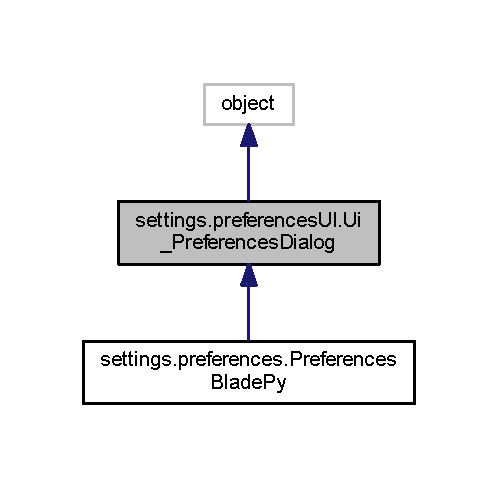
\includegraphics[width=239pt]{classsettings_1_1preferences_u_i_1_1_ui___preferences_dialog__inherit__graph}
\end{center}
\end{figure}
\subsection*{Public Member Functions}
\begin{DoxyCompactItemize}
\item 
def \hyperlink{classsettings_1_1preferences_u_i_1_1_ui___preferences_dialog_a61eadae581e6b31932e65f89ee78760c}{setup\+Ui} (self, \hyperlink{namespacesettings_1_1preferences_u_i_a70162ca377a00273f0795162093f7958}{Preferences\+Dialog})
\item 
def \hyperlink{classsettings_1_1preferences_u_i_1_1_ui___preferences_dialog_a29096d3ca31a6d880f3e4680987243e8}{retranslate\+Ui} (self, \hyperlink{namespacesettings_1_1preferences_u_i_a70162ca377a00273f0795162093f7958}{Preferences\+Dialog})
\end{DoxyCompactItemize}
\subsection*{Public Attributes}
\begin{DoxyCompactItemize}
\item 
\hyperlink{classsettings_1_1preferences_u_i_1_1_ui___preferences_dialog_ad769696a12317c7f92ed3366311bc496}{vertical\+Layout}
\item 
\hyperlink{classsettings_1_1preferences_u_i_1_1_ui___preferences_dialog_aefabfa9bb4d3ece796fee13c167d52fc}{ui\+\_\+preferences\+\_\+tab}
\item 
\hyperlink{classsettings_1_1preferences_u_i_1_1_ui___preferences_dialog_a0f603694eed0cda9d39a0d9bc19c2e10}{ui\+\_\+preferences\+\_\+general\+\_\+tab}
\item 
\hyperlink{classsettings_1_1preferences_u_i_1_1_ui___preferences_dialog_af50058d66700f51fb46a0bab1cf0aa4b}{vertical\+Layout\+\_\+2}
\item 
\hyperlink{classsettings_1_1preferences_u_i_1_1_ui___preferences_dialog_adca7b98e8183192a5fc165c8695d44f5}{ui\+\_\+preferences\+\_\+general\+\_\+groupbox}
\item 
\hyperlink{classsettings_1_1preferences_u_i_1_1_ui___preferences_dialog_a9758be9a7207723c709109813da770fb}{grid\+Layout}
\item 
\hyperlink{classsettings_1_1preferences_u_i_1_1_ui___preferences_dialog_a2dbc9c7187826d35dfb423e2536031c1}{self\+\_\+preferences\+\_\+general\+\_\+outputs\+\_\+groupbox}
\item 
\hyperlink{classsettings_1_1preferences_u_i_1_1_ui___preferences_dialog_af17928a62255c96603422710076dbede}{vertical\+Layout\+\_\+4}
\item 
\hyperlink{classsettings_1_1preferences_u_i_1_1_ui___preferences_dialog_a47018f6a822750d843c3ba200c5dfdd5}{ui\+\_\+preferences\+\_\+general\+\_\+outputs\+\_\+description\+\_\+lbl}
\item 
\hyperlink{classsettings_1_1preferences_u_i_1_1_ui___preferences_dialog_aec77d619b1316cf81f501262151d4388}{self\+\_\+preferences\+\_\+general\+\_\+outputs\+\_\+gl}
\item 
\hyperlink{classsettings_1_1preferences_u_i_1_1_ui___preferences_dialog_a99ea63136960e76164e086bee4b6acb5}{ui\+\_\+preferences\+\_\+tecplot\+\_\+2d\+\_\+chk}
\item 
\hyperlink{classsettings_1_1preferences_u_i_1_1_ui___preferences_dialog_ab28264229e6a9e05bf21541ed645dcb2}{ui\+\_\+preferences\+\_\+igs\+\_\+3d\+\_\+cur\+\_\+exception\+\_\+edit}
\item 
\hyperlink{classsettings_1_1preferences_u_i_1_1_ui___preferences_dialog_a1ce10779ded45f28b6afd571de7c1dc4}{ui\+\_\+preferences\+\_\+igs\+\_\+2d\+\_\+cur\+\_\+chk}
\item 
\hyperlink{classsettings_1_1preferences_u_i_1_1_ui___preferences_dialog_af72b1a9124fb421c1fbe62adb174fe77}{ui\+\_\+preferences\+\_\+igs\+\_\+3d\+\_\+cur\+\_\+chk}
\item 
\hyperlink{classsettings_1_1preferences_u_i_1_1_ui___preferences_dialog_a6ff22661fcefd7225763bd7655ceb36c}{ui\+\_\+preferences\+\_\+igs\+\_\+surf\+\_\+chk}
\item 
\hyperlink{classsettings_1_1preferences_u_i_1_1_ui___preferences_dialog_a4e600e40407001e5ea272f73f359cde8}{ui\+\_\+preferences\+\_\+igs\+\_\+2d\+\_\+cur\+\_\+exception\+\_\+edit}
\item 
\hyperlink{classsettings_1_1preferences_u_i_1_1_ui___preferences_dialog_a420fe65d048f3d9f4c464f5426f72928}{ui\+\_\+preferences\+\_\+igs\+\_\+surf\+\_\+exception\+\_\+edit}
\item 
\hyperlink{classsettings_1_1preferences_u_i_1_1_ui___preferences_dialog_a58f750a42bbb7ed7e89fe15f5883bf3d}{self\+\_\+preferences\+\_\+general\+\_\+shape\+\_\+groupbox}
\item 
\hyperlink{classsettings_1_1preferences_u_i_1_1_ui___preferences_dialog_a6cf68c068ac0041c158fb99804e4f6b2}{vertical\+Layout\+\_\+3}
\item 
\hyperlink{classsettings_1_1preferences_u_i_1_1_ui___preferences_dialog_a44174aad3cbdfd15fed7998607c98f74}{ui\+\_\+preferences\+\_\+general\+\_\+shape\+\_\+gl}
\item 
\hyperlink{classsettings_1_1preferences_u_i_1_1_ui___preferences_dialog_a0b043ee35d1213137f70620301f00d5f}{ui\+\_\+preferences\+\_\+default\+\_\+color\+\_\+combo}
\item 
\hyperlink{classsettings_1_1preferences_u_i_1_1_ui___preferences_dialog_a018f3104e4bb1e4f93acdb919f43d4a7}{ui\+\_\+preferences\+\_\+default\+\_\+quality\+\_\+dspn}
\item 
\hyperlink{classsettings_1_1preferences_u_i_1_1_ui___preferences_dialog_a87156afaeff8f61b423a3b7cafc07619}{ui\+\_\+preferences\+\_\+default\+\_\+transparency\+\_\+dspn}
\item 
\hyperlink{classsettings_1_1preferences_u_i_1_1_ui___preferences_dialog_af4af1d948631ab4e16506f3dc6ad476d}{ui\+\_\+preferences\+\_\+transparency\+\_\+lbl\+\_\+2}
\item 
\hyperlink{classsettings_1_1preferences_u_i_1_1_ui___preferences_dialog_a2469ae136e448dd1df44686ae61f5f01}{ui\+\_\+preferences\+\_\+default\+\_\+color\+\_\+lbl}
\item 
\hyperlink{classsettings_1_1preferences_u_i_1_1_ui___preferences_dialog_a243905c4e84872947db1bb8dcedadda4}{ui\+\_\+preferences\+\_\+transparency\+\_\+lbl}
\item 
\hyperlink{classsettings_1_1preferences_u_i_1_1_ui___preferences_dialog_a24dafe3bdccfb5c2439cca09d041f8e2}{self\+\_\+preferences\+\_\+general\+\_\+display\+\_\+groupbox}
\item 
\hyperlink{classsettings_1_1preferences_u_i_1_1_ui___preferences_dialog_a770a35129466bdc08cfc70c1a31d74d0}{vertical\+Layout\+\_\+5}
\item 
\hyperlink{classsettings_1_1preferences_u_i_1_1_ui___preferences_dialog_a34e66b85aedb9d531bd13e099c4abd17}{self\+\_\+preferences\+\_\+general\+\_\+display\+\_\+gl}
\item 
\hyperlink{classsettings_1_1preferences_u_i_1_1_ui___preferences_dialog_ab9f4bd205de45a28fb6df5fd10a11e13}{ui\+\_\+preferences\+\_\+zoom\+\_\+dpsn}
\item 
\hyperlink{classsettings_1_1preferences_u_i_1_1_ui___preferences_dialog_a8321ca1cf385acdcd4a23a9aeba71982}{ui\+\_\+preferences\+\_\+zoom\+\_\+lbl}
\item 
\hyperlink{classsettings_1_1preferences_u_i_1_1_ui___preferences_dialog_abeeea5dce817fab1714dcfea02931865}{ui\+\_\+preferences\+\_\+okcancelapply\+\_\+hl}
\item 
\hyperlink{classsettings_1_1preferences_u_i_1_1_ui___preferences_dialog_a191d2ad10ffb160b79b7795e05fe37e3}{ui\+\_\+preferences\+\_\+ok\+\_\+btn}
\item 
\hyperlink{classsettings_1_1preferences_u_i_1_1_ui___preferences_dialog_a47ad79d67a89e77f0cf358171fac15b2}{ui\+\_\+preferences\+\_\+cancel\+\_\+btn}
\item 
\hyperlink{classsettings_1_1preferences_u_i_1_1_ui___preferences_dialog_a3f0de42b6f49c050f03b806cfc7541f7}{ui\+\_\+preferences\+\_\+apply\+\_\+btn}
\end{DoxyCompactItemize}


\subsection{Member Function Documentation}
\hypertarget{classsettings_1_1preferences_u_i_1_1_ui___preferences_dialog_a29096d3ca31a6d880f3e4680987243e8}{}\label{classsettings_1_1preferences_u_i_1_1_ui___preferences_dialog_a29096d3ca31a6d880f3e4680987243e8} 
\index{settings\+::preferences\+U\+I\+::\+Ui\+\_\+\+Preferences\+Dialog@{settings\+::preferences\+U\+I\+::\+Ui\+\_\+\+Preferences\+Dialog}!retranslate\+Ui@{retranslate\+Ui}}
\index{retranslate\+Ui@{retranslate\+Ui}!settings\+::preferences\+U\+I\+::\+Ui\+\_\+\+Preferences\+Dialog@{settings\+::preferences\+U\+I\+::\+Ui\+\_\+\+Preferences\+Dialog}}
\subsubsection{\texorpdfstring{retranslate\+Ui()}{retranslateUi()}}
{\footnotesize\ttfamily def settings.\+preferences\+U\+I.\+Ui\+\_\+\+Preferences\+Dialog.\+retranslate\+Ui (\begin{DoxyParamCaption}\item[{}]{self,  }\item[{}]{Preferences\+Dialog }\end{DoxyParamCaption})}

\hypertarget{classsettings_1_1preferences_u_i_1_1_ui___preferences_dialog_a61eadae581e6b31932e65f89ee78760c}{}\label{classsettings_1_1preferences_u_i_1_1_ui___preferences_dialog_a61eadae581e6b31932e65f89ee78760c} 
\index{settings\+::preferences\+U\+I\+::\+Ui\+\_\+\+Preferences\+Dialog@{settings\+::preferences\+U\+I\+::\+Ui\+\_\+\+Preferences\+Dialog}!setup\+Ui@{setup\+Ui}}
\index{setup\+Ui@{setup\+Ui}!settings\+::preferences\+U\+I\+::\+Ui\+\_\+\+Preferences\+Dialog@{settings\+::preferences\+U\+I\+::\+Ui\+\_\+\+Preferences\+Dialog}}
\subsubsection{\texorpdfstring{setup\+Ui()}{setupUi()}}
{\footnotesize\ttfamily def settings.\+preferences\+U\+I.\+Ui\+\_\+\+Preferences\+Dialog.\+setup\+Ui (\begin{DoxyParamCaption}\item[{}]{self,  }\item[{}]{Preferences\+Dialog }\end{DoxyParamCaption})}



\subsection{Member Data Documentation}
\hypertarget{classsettings_1_1preferences_u_i_1_1_ui___preferences_dialog_a9758be9a7207723c709109813da770fb}{}\label{classsettings_1_1preferences_u_i_1_1_ui___preferences_dialog_a9758be9a7207723c709109813da770fb} 
\index{settings\+::preferences\+U\+I\+::\+Ui\+\_\+\+Preferences\+Dialog@{settings\+::preferences\+U\+I\+::\+Ui\+\_\+\+Preferences\+Dialog}!grid\+Layout@{grid\+Layout}}
\index{grid\+Layout@{grid\+Layout}!settings\+::preferences\+U\+I\+::\+Ui\+\_\+\+Preferences\+Dialog@{settings\+::preferences\+U\+I\+::\+Ui\+\_\+\+Preferences\+Dialog}}
\subsubsection{\texorpdfstring{grid\+Layout}{gridLayout}}
{\footnotesize\ttfamily settings.\+preferences\+U\+I.\+Ui\+\_\+\+Preferences\+Dialog.\+grid\+Layout}

\hypertarget{classsettings_1_1preferences_u_i_1_1_ui___preferences_dialog_a34e66b85aedb9d531bd13e099c4abd17}{}\label{classsettings_1_1preferences_u_i_1_1_ui___preferences_dialog_a34e66b85aedb9d531bd13e099c4abd17} 
\index{settings\+::preferences\+U\+I\+::\+Ui\+\_\+\+Preferences\+Dialog@{settings\+::preferences\+U\+I\+::\+Ui\+\_\+\+Preferences\+Dialog}!self\+\_\+preferences\+\_\+general\+\_\+display\+\_\+gl@{self\+\_\+preferences\+\_\+general\+\_\+display\+\_\+gl}}
\index{self\+\_\+preferences\+\_\+general\+\_\+display\+\_\+gl@{self\+\_\+preferences\+\_\+general\+\_\+display\+\_\+gl}!settings\+::preferences\+U\+I\+::\+Ui\+\_\+\+Preferences\+Dialog@{settings\+::preferences\+U\+I\+::\+Ui\+\_\+\+Preferences\+Dialog}}
\subsubsection{\texorpdfstring{self\+\_\+preferences\+\_\+general\+\_\+display\+\_\+gl}{self\_preferences\_general\_display\_gl}}
{\footnotesize\ttfamily settings.\+preferences\+U\+I.\+Ui\+\_\+\+Preferences\+Dialog.\+self\+\_\+preferences\+\_\+general\+\_\+display\+\_\+gl}

\hypertarget{classsettings_1_1preferences_u_i_1_1_ui___preferences_dialog_a24dafe3bdccfb5c2439cca09d041f8e2}{}\label{classsettings_1_1preferences_u_i_1_1_ui___preferences_dialog_a24dafe3bdccfb5c2439cca09d041f8e2} 
\index{settings\+::preferences\+U\+I\+::\+Ui\+\_\+\+Preferences\+Dialog@{settings\+::preferences\+U\+I\+::\+Ui\+\_\+\+Preferences\+Dialog}!self\+\_\+preferences\+\_\+general\+\_\+display\+\_\+groupbox@{self\+\_\+preferences\+\_\+general\+\_\+display\+\_\+groupbox}}
\index{self\+\_\+preferences\+\_\+general\+\_\+display\+\_\+groupbox@{self\+\_\+preferences\+\_\+general\+\_\+display\+\_\+groupbox}!settings\+::preferences\+U\+I\+::\+Ui\+\_\+\+Preferences\+Dialog@{settings\+::preferences\+U\+I\+::\+Ui\+\_\+\+Preferences\+Dialog}}
\subsubsection{\texorpdfstring{self\+\_\+preferences\+\_\+general\+\_\+display\+\_\+groupbox}{self\_preferences\_general\_display\_groupbox}}
{\footnotesize\ttfamily settings.\+preferences\+U\+I.\+Ui\+\_\+\+Preferences\+Dialog.\+self\+\_\+preferences\+\_\+general\+\_\+display\+\_\+groupbox}

\hypertarget{classsettings_1_1preferences_u_i_1_1_ui___preferences_dialog_aec77d619b1316cf81f501262151d4388}{}\label{classsettings_1_1preferences_u_i_1_1_ui___preferences_dialog_aec77d619b1316cf81f501262151d4388} 
\index{settings\+::preferences\+U\+I\+::\+Ui\+\_\+\+Preferences\+Dialog@{settings\+::preferences\+U\+I\+::\+Ui\+\_\+\+Preferences\+Dialog}!self\+\_\+preferences\+\_\+general\+\_\+outputs\+\_\+gl@{self\+\_\+preferences\+\_\+general\+\_\+outputs\+\_\+gl}}
\index{self\+\_\+preferences\+\_\+general\+\_\+outputs\+\_\+gl@{self\+\_\+preferences\+\_\+general\+\_\+outputs\+\_\+gl}!settings\+::preferences\+U\+I\+::\+Ui\+\_\+\+Preferences\+Dialog@{settings\+::preferences\+U\+I\+::\+Ui\+\_\+\+Preferences\+Dialog}}
\subsubsection{\texorpdfstring{self\+\_\+preferences\+\_\+general\+\_\+outputs\+\_\+gl}{self\_preferences\_general\_outputs\_gl}}
{\footnotesize\ttfamily settings.\+preferences\+U\+I.\+Ui\+\_\+\+Preferences\+Dialog.\+self\+\_\+preferences\+\_\+general\+\_\+outputs\+\_\+gl}

\hypertarget{classsettings_1_1preferences_u_i_1_1_ui___preferences_dialog_a2dbc9c7187826d35dfb423e2536031c1}{}\label{classsettings_1_1preferences_u_i_1_1_ui___preferences_dialog_a2dbc9c7187826d35dfb423e2536031c1} 
\index{settings\+::preferences\+U\+I\+::\+Ui\+\_\+\+Preferences\+Dialog@{settings\+::preferences\+U\+I\+::\+Ui\+\_\+\+Preferences\+Dialog}!self\+\_\+preferences\+\_\+general\+\_\+outputs\+\_\+groupbox@{self\+\_\+preferences\+\_\+general\+\_\+outputs\+\_\+groupbox}}
\index{self\+\_\+preferences\+\_\+general\+\_\+outputs\+\_\+groupbox@{self\+\_\+preferences\+\_\+general\+\_\+outputs\+\_\+groupbox}!settings\+::preferences\+U\+I\+::\+Ui\+\_\+\+Preferences\+Dialog@{settings\+::preferences\+U\+I\+::\+Ui\+\_\+\+Preferences\+Dialog}}
\subsubsection{\texorpdfstring{self\+\_\+preferences\+\_\+general\+\_\+outputs\+\_\+groupbox}{self\_preferences\_general\_outputs\_groupbox}}
{\footnotesize\ttfamily settings.\+preferences\+U\+I.\+Ui\+\_\+\+Preferences\+Dialog.\+self\+\_\+preferences\+\_\+general\+\_\+outputs\+\_\+groupbox}

\hypertarget{classsettings_1_1preferences_u_i_1_1_ui___preferences_dialog_a58f750a42bbb7ed7e89fe15f5883bf3d}{}\label{classsettings_1_1preferences_u_i_1_1_ui___preferences_dialog_a58f750a42bbb7ed7e89fe15f5883bf3d} 
\index{settings\+::preferences\+U\+I\+::\+Ui\+\_\+\+Preferences\+Dialog@{settings\+::preferences\+U\+I\+::\+Ui\+\_\+\+Preferences\+Dialog}!self\+\_\+preferences\+\_\+general\+\_\+shape\+\_\+groupbox@{self\+\_\+preferences\+\_\+general\+\_\+shape\+\_\+groupbox}}
\index{self\+\_\+preferences\+\_\+general\+\_\+shape\+\_\+groupbox@{self\+\_\+preferences\+\_\+general\+\_\+shape\+\_\+groupbox}!settings\+::preferences\+U\+I\+::\+Ui\+\_\+\+Preferences\+Dialog@{settings\+::preferences\+U\+I\+::\+Ui\+\_\+\+Preferences\+Dialog}}
\subsubsection{\texorpdfstring{self\+\_\+preferences\+\_\+general\+\_\+shape\+\_\+groupbox}{self\_preferences\_general\_shape\_groupbox}}
{\footnotesize\ttfamily settings.\+preferences\+U\+I.\+Ui\+\_\+\+Preferences\+Dialog.\+self\+\_\+preferences\+\_\+general\+\_\+shape\+\_\+groupbox}

\hypertarget{classsettings_1_1preferences_u_i_1_1_ui___preferences_dialog_a3f0de42b6f49c050f03b806cfc7541f7}{}\label{classsettings_1_1preferences_u_i_1_1_ui___preferences_dialog_a3f0de42b6f49c050f03b806cfc7541f7} 
\index{settings\+::preferences\+U\+I\+::\+Ui\+\_\+\+Preferences\+Dialog@{settings\+::preferences\+U\+I\+::\+Ui\+\_\+\+Preferences\+Dialog}!ui\+\_\+preferences\+\_\+apply\+\_\+btn@{ui\+\_\+preferences\+\_\+apply\+\_\+btn}}
\index{ui\+\_\+preferences\+\_\+apply\+\_\+btn@{ui\+\_\+preferences\+\_\+apply\+\_\+btn}!settings\+::preferences\+U\+I\+::\+Ui\+\_\+\+Preferences\+Dialog@{settings\+::preferences\+U\+I\+::\+Ui\+\_\+\+Preferences\+Dialog}}
\subsubsection{\texorpdfstring{ui\+\_\+preferences\+\_\+apply\+\_\+btn}{ui\_preferences\_apply\_btn}}
{\footnotesize\ttfamily settings.\+preferences\+U\+I.\+Ui\+\_\+\+Preferences\+Dialog.\+ui\+\_\+preferences\+\_\+apply\+\_\+btn}

\hypertarget{classsettings_1_1preferences_u_i_1_1_ui___preferences_dialog_a47ad79d67a89e77f0cf358171fac15b2}{}\label{classsettings_1_1preferences_u_i_1_1_ui___preferences_dialog_a47ad79d67a89e77f0cf358171fac15b2} 
\index{settings\+::preferences\+U\+I\+::\+Ui\+\_\+\+Preferences\+Dialog@{settings\+::preferences\+U\+I\+::\+Ui\+\_\+\+Preferences\+Dialog}!ui\+\_\+preferences\+\_\+cancel\+\_\+btn@{ui\+\_\+preferences\+\_\+cancel\+\_\+btn}}
\index{ui\+\_\+preferences\+\_\+cancel\+\_\+btn@{ui\+\_\+preferences\+\_\+cancel\+\_\+btn}!settings\+::preferences\+U\+I\+::\+Ui\+\_\+\+Preferences\+Dialog@{settings\+::preferences\+U\+I\+::\+Ui\+\_\+\+Preferences\+Dialog}}
\subsubsection{\texorpdfstring{ui\+\_\+preferences\+\_\+cancel\+\_\+btn}{ui\_preferences\_cancel\_btn}}
{\footnotesize\ttfamily settings.\+preferences\+U\+I.\+Ui\+\_\+\+Preferences\+Dialog.\+ui\+\_\+preferences\+\_\+cancel\+\_\+btn}

\hypertarget{classsettings_1_1preferences_u_i_1_1_ui___preferences_dialog_a0b043ee35d1213137f70620301f00d5f}{}\label{classsettings_1_1preferences_u_i_1_1_ui___preferences_dialog_a0b043ee35d1213137f70620301f00d5f} 
\index{settings\+::preferences\+U\+I\+::\+Ui\+\_\+\+Preferences\+Dialog@{settings\+::preferences\+U\+I\+::\+Ui\+\_\+\+Preferences\+Dialog}!ui\+\_\+preferences\+\_\+default\+\_\+color\+\_\+combo@{ui\+\_\+preferences\+\_\+default\+\_\+color\+\_\+combo}}
\index{ui\+\_\+preferences\+\_\+default\+\_\+color\+\_\+combo@{ui\+\_\+preferences\+\_\+default\+\_\+color\+\_\+combo}!settings\+::preferences\+U\+I\+::\+Ui\+\_\+\+Preferences\+Dialog@{settings\+::preferences\+U\+I\+::\+Ui\+\_\+\+Preferences\+Dialog}}
\subsubsection{\texorpdfstring{ui\+\_\+preferences\+\_\+default\+\_\+color\+\_\+combo}{ui\_preferences\_default\_color\_combo}}
{\footnotesize\ttfamily settings.\+preferences\+U\+I.\+Ui\+\_\+\+Preferences\+Dialog.\+ui\+\_\+preferences\+\_\+default\+\_\+color\+\_\+combo}

\hypertarget{classsettings_1_1preferences_u_i_1_1_ui___preferences_dialog_a2469ae136e448dd1df44686ae61f5f01}{}\label{classsettings_1_1preferences_u_i_1_1_ui___preferences_dialog_a2469ae136e448dd1df44686ae61f5f01} 
\index{settings\+::preferences\+U\+I\+::\+Ui\+\_\+\+Preferences\+Dialog@{settings\+::preferences\+U\+I\+::\+Ui\+\_\+\+Preferences\+Dialog}!ui\+\_\+preferences\+\_\+default\+\_\+color\+\_\+lbl@{ui\+\_\+preferences\+\_\+default\+\_\+color\+\_\+lbl}}
\index{ui\+\_\+preferences\+\_\+default\+\_\+color\+\_\+lbl@{ui\+\_\+preferences\+\_\+default\+\_\+color\+\_\+lbl}!settings\+::preferences\+U\+I\+::\+Ui\+\_\+\+Preferences\+Dialog@{settings\+::preferences\+U\+I\+::\+Ui\+\_\+\+Preferences\+Dialog}}
\subsubsection{\texorpdfstring{ui\+\_\+preferences\+\_\+default\+\_\+color\+\_\+lbl}{ui\_preferences\_default\_color\_lbl}}
{\footnotesize\ttfamily settings.\+preferences\+U\+I.\+Ui\+\_\+\+Preferences\+Dialog.\+ui\+\_\+preferences\+\_\+default\+\_\+color\+\_\+lbl}

\hypertarget{classsettings_1_1preferences_u_i_1_1_ui___preferences_dialog_a018f3104e4bb1e4f93acdb919f43d4a7}{}\label{classsettings_1_1preferences_u_i_1_1_ui___preferences_dialog_a018f3104e4bb1e4f93acdb919f43d4a7} 
\index{settings\+::preferences\+U\+I\+::\+Ui\+\_\+\+Preferences\+Dialog@{settings\+::preferences\+U\+I\+::\+Ui\+\_\+\+Preferences\+Dialog}!ui\+\_\+preferences\+\_\+default\+\_\+quality\+\_\+dspn@{ui\+\_\+preferences\+\_\+default\+\_\+quality\+\_\+dspn}}
\index{ui\+\_\+preferences\+\_\+default\+\_\+quality\+\_\+dspn@{ui\+\_\+preferences\+\_\+default\+\_\+quality\+\_\+dspn}!settings\+::preferences\+U\+I\+::\+Ui\+\_\+\+Preferences\+Dialog@{settings\+::preferences\+U\+I\+::\+Ui\+\_\+\+Preferences\+Dialog}}
\subsubsection{\texorpdfstring{ui\+\_\+preferences\+\_\+default\+\_\+quality\+\_\+dspn}{ui\_preferences\_default\_quality\_dspn}}
{\footnotesize\ttfamily settings.\+preferences\+U\+I.\+Ui\+\_\+\+Preferences\+Dialog.\+ui\+\_\+preferences\+\_\+default\+\_\+quality\+\_\+dspn}

\hypertarget{classsettings_1_1preferences_u_i_1_1_ui___preferences_dialog_a87156afaeff8f61b423a3b7cafc07619}{}\label{classsettings_1_1preferences_u_i_1_1_ui___preferences_dialog_a87156afaeff8f61b423a3b7cafc07619} 
\index{settings\+::preferences\+U\+I\+::\+Ui\+\_\+\+Preferences\+Dialog@{settings\+::preferences\+U\+I\+::\+Ui\+\_\+\+Preferences\+Dialog}!ui\+\_\+preferences\+\_\+default\+\_\+transparency\+\_\+dspn@{ui\+\_\+preferences\+\_\+default\+\_\+transparency\+\_\+dspn}}
\index{ui\+\_\+preferences\+\_\+default\+\_\+transparency\+\_\+dspn@{ui\+\_\+preferences\+\_\+default\+\_\+transparency\+\_\+dspn}!settings\+::preferences\+U\+I\+::\+Ui\+\_\+\+Preferences\+Dialog@{settings\+::preferences\+U\+I\+::\+Ui\+\_\+\+Preferences\+Dialog}}
\subsubsection{\texorpdfstring{ui\+\_\+preferences\+\_\+default\+\_\+transparency\+\_\+dspn}{ui\_preferences\_default\_transparency\_dspn}}
{\footnotesize\ttfamily settings.\+preferences\+U\+I.\+Ui\+\_\+\+Preferences\+Dialog.\+ui\+\_\+preferences\+\_\+default\+\_\+transparency\+\_\+dspn}

\hypertarget{classsettings_1_1preferences_u_i_1_1_ui___preferences_dialog_adca7b98e8183192a5fc165c8695d44f5}{}\label{classsettings_1_1preferences_u_i_1_1_ui___preferences_dialog_adca7b98e8183192a5fc165c8695d44f5} 
\index{settings\+::preferences\+U\+I\+::\+Ui\+\_\+\+Preferences\+Dialog@{settings\+::preferences\+U\+I\+::\+Ui\+\_\+\+Preferences\+Dialog}!ui\+\_\+preferences\+\_\+general\+\_\+groupbox@{ui\+\_\+preferences\+\_\+general\+\_\+groupbox}}
\index{ui\+\_\+preferences\+\_\+general\+\_\+groupbox@{ui\+\_\+preferences\+\_\+general\+\_\+groupbox}!settings\+::preferences\+U\+I\+::\+Ui\+\_\+\+Preferences\+Dialog@{settings\+::preferences\+U\+I\+::\+Ui\+\_\+\+Preferences\+Dialog}}
\subsubsection{\texorpdfstring{ui\+\_\+preferences\+\_\+general\+\_\+groupbox}{ui\_preferences\_general\_groupbox}}
{\footnotesize\ttfamily settings.\+preferences\+U\+I.\+Ui\+\_\+\+Preferences\+Dialog.\+ui\+\_\+preferences\+\_\+general\+\_\+groupbox}

\hypertarget{classsettings_1_1preferences_u_i_1_1_ui___preferences_dialog_a47018f6a822750d843c3ba200c5dfdd5}{}\label{classsettings_1_1preferences_u_i_1_1_ui___preferences_dialog_a47018f6a822750d843c3ba200c5dfdd5} 
\index{settings\+::preferences\+U\+I\+::\+Ui\+\_\+\+Preferences\+Dialog@{settings\+::preferences\+U\+I\+::\+Ui\+\_\+\+Preferences\+Dialog}!ui\+\_\+preferences\+\_\+general\+\_\+outputs\+\_\+description\+\_\+lbl@{ui\+\_\+preferences\+\_\+general\+\_\+outputs\+\_\+description\+\_\+lbl}}
\index{ui\+\_\+preferences\+\_\+general\+\_\+outputs\+\_\+description\+\_\+lbl@{ui\+\_\+preferences\+\_\+general\+\_\+outputs\+\_\+description\+\_\+lbl}!settings\+::preferences\+U\+I\+::\+Ui\+\_\+\+Preferences\+Dialog@{settings\+::preferences\+U\+I\+::\+Ui\+\_\+\+Preferences\+Dialog}}
\subsubsection{\texorpdfstring{ui\+\_\+preferences\+\_\+general\+\_\+outputs\+\_\+description\+\_\+lbl}{ui\_preferences\_general\_outputs\_description\_lbl}}
{\footnotesize\ttfamily settings.\+preferences\+U\+I.\+Ui\+\_\+\+Preferences\+Dialog.\+ui\+\_\+preferences\+\_\+general\+\_\+outputs\+\_\+description\+\_\+lbl}

\hypertarget{classsettings_1_1preferences_u_i_1_1_ui___preferences_dialog_a44174aad3cbdfd15fed7998607c98f74}{}\label{classsettings_1_1preferences_u_i_1_1_ui___preferences_dialog_a44174aad3cbdfd15fed7998607c98f74} 
\index{settings\+::preferences\+U\+I\+::\+Ui\+\_\+\+Preferences\+Dialog@{settings\+::preferences\+U\+I\+::\+Ui\+\_\+\+Preferences\+Dialog}!ui\+\_\+preferences\+\_\+general\+\_\+shape\+\_\+gl@{ui\+\_\+preferences\+\_\+general\+\_\+shape\+\_\+gl}}
\index{ui\+\_\+preferences\+\_\+general\+\_\+shape\+\_\+gl@{ui\+\_\+preferences\+\_\+general\+\_\+shape\+\_\+gl}!settings\+::preferences\+U\+I\+::\+Ui\+\_\+\+Preferences\+Dialog@{settings\+::preferences\+U\+I\+::\+Ui\+\_\+\+Preferences\+Dialog}}
\subsubsection{\texorpdfstring{ui\+\_\+preferences\+\_\+general\+\_\+shape\+\_\+gl}{ui\_preferences\_general\_shape\_gl}}
{\footnotesize\ttfamily settings.\+preferences\+U\+I.\+Ui\+\_\+\+Preferences\+Dialog.\+ui\+\_\+preferences\+\_\+general\+\_\+shape\+\_\+gl}

\hypertarget{classsettings_1_1preferences_u_i_1_1_ui___preferences_dialog_a0f603694eed0cda9d39a0d9bc19c2e10}{}\label{classsettings_1_1preferences_u_i_1_1_ui___preferences_dialog_a0f603694eed0cda9d39a0d9bc19c2e10} 
\index{settings\+::preferences\+U\+I\+::\+Ui\+\_\+\+Preferences\+Dialog@{settings\+::preferences\+U\+I\+::\+Ui\+\_\+\+Preferences\+Dialog}!ui\+\_\+preferences\+\_\+general\+\_\+tab@{ui\+\_\+preferences\+\_\+general\+\_\+tab}}
\index{ui\+\_\+preferences\+\_\+general\+\_\+tab@{ui\+\_\+preferences\+\_\+general\+\_\+tab}!settings\+::preferences\+U\+I\+::\+Ui\+\_\+\+Preferences\+Dialog@{settings\+::preferences\+U\+I\+::\+Ui\+\_\+\+Preferences\+Dialog}}
\subsubsection{\texorpdfstring{ui\+\_\+preferences\+\_\+general\+\_\+tab}{ui\_preferences\_general\_tab}}
{\footnotesize\ttfamily settings.\+preferences\+U\+I.\+Ui\+\_\+\+Preferences\+Dialog.\+ui\+\_\+preferences\+\_\+general\+\_\+tab}

\hypertarget{classsettings_1_1preferences_u_i_1_1_ui___preferences_dialog_a1ce10779ded45f28b6afd571de7c1dc4}{}\label{classsettings_1_1preferences_u_i_1_1_ui___preferences_dialog_a1ce10779ded45f28b6afd571de7c1dc4} 
\index{settings\+::preferences\+U\+I\+::\+Ui\+\_\+\+Preferences\+Dialog@{settings\+::preferences\+U\+I\+::\+Ui\+\_\+\+Preferences\+Dialog}!ui\+\_\+preferences\+\_\+igs\+\_\+2d\+\_\+cur\+\_\+chk@{ui\+\_\+preferences\+\_\+igs\+\_\+2d\+\_\+cur\+\_\+chk}}
\index{ui\+\_\+preferences\+\_\+igs\+\_\+2d\+\_\+cur\+\_\+chk@{ui\+\_\+preferences\+\_\+igs\+\_\+2d\+\_\+cur\+\_\+chk}!settings\+::preferences\+U\+I\+::\+Ui\+\_\+\+Preferences\+Dialog@{settings\+::preferences\+U\+I\+::\+Ui\+\_\+\+Preferences\+Dialog}}
\subsubsection{\texorpdfstring{ui\+\_\+preferences\+\_\+igs\+\_\+2d\+\_\+cur\+\_\+chk}{ui\_preferences\_igs\_2d\_cur\_chk}}
{\footnotesize\ttfamily settings.\+preferences\+U\+I.\+Ui\+\_\+\+Preferences\+Dialog.\+ui\+\_\+preferences\+\_\+igs\+\_\+2d\+\_\+cur\+\_\+chk}

\hypertarget{classsettings_1_1preferences_u_i_1_1_ui___preferences_dialog_a4e600e40407001e5ea272f73f359cde8}{}\label{classsettings_1_1preferences_u_i_1_1_ui___preferences_dialog_a4e600e40407001e5ea272f73f359cde8} 
\index{settings\+::preferences\+U\+I\+::\+Ui\+\_\+\+Preferences\+Dialog@{settings\+::preferences\+U\+I\+::\+Ui\+\_\+\+Preferences\+Dialog}!ui\+\_\+preferences\+\_\+igs\+\_\+2d\+\_\+cur\+\_\+exception\+\_\+edit@{ui\+\_\+preferences\+\_\+igs\+\_\+2d\+\_\+cur\+\_\+exception\+\_\+edit}}
\index{ui\+\_\+preferences\+\_\+igs\+\_\+2d\+\_\+cur\+\_\+exception\+\_\+edit@{ui\+\_\+preferences\+\_\+igs\+\_\+2d\+\_\+cur\+\_\+exception\+\_\+edit}!settings\+::preferences\+U\+I\+::\+Ui\+\_\+\+Preferences\+Dialog@{settings\+::preferences\+U\+I\+::\+Ui\+\_\+\+Preferences\+Dialog}}
\subsubsection{\texorpdfstring{ui\+\_\+preferences\+\_\+igs\+\_\+2d\+\_\+cur\+\_\+exception\+\_\+edit}{ui\_preferences\_igs\_2d\_cur\_exception\_edit}}
{\footnotesize\ttfamily settings.\+preferences\+U\+I.\+Ui\+\_\+\+Preferences\+Dialog.\+ui\+\_\+preferences\+\_\+igs\+\_\+2d\+\_\+cur\+\_\+exception\+\_\+edit}

\hypertarget{classsettings_1_1preferences_u_i_1_1_ui___preferences_dialog_af72b1a9124fb421c1fbe62adb174fe77}{}\label{classsettings_1_1preferences_u_i_1_1_ui___preferences_dialog_af72b1a9124fb421c1fbe62adb174fe77} 
\index{settings\+::preferences\+U\+I\+::\+Ui\+\_\+\+Preferences\+Dialog@{settings\+::preferences\+U\+I\+::\+Ui\+\_\+\+Preferences\+Dialog}!ui\+\_\+preferences\+\_\+igs\+\_\+3d\+\_\+cur\+\_\+chk@{ui\+\_\+preferences\+\_\+igs\+\_\+3d\+\_\+cur\+\_\+chk}}
\index{ui\+\_\+preferences\+\_\+igs\+\_\+3d\+\_\+cur\+\_\+chk@{ui\+\_\+preferences\+\_\+igs\+\_\+3d\+\_\+cur\+\_\+chk}!settings\+::preferences\+U\+I\+::\+Ui\+\_\+\+Preferences\+Dialog@{settings\+::preferences\+U\+I\+::\+Ui\+\_\+\+Preferences\+Dialog}}
\subsubsection{\texorpdfstring{ui\+\_\+preferences\+\_\+igs\+\_\+3d\+\_\+cur\+\_\+chk}{ui\_preferences\_igs\_3d\_cur\_chk}}
{\footnotesize\ttfamily settings.\+preferences\+U\+I.\+Ui\+\_\+\+Preferences\+Dialog.\+ui\+\_\+preferences\+\_\+igs\+\_\+3d\+\_\+cur\+\_\+chk}

\hypertarget{classsettings_1_1preferences_u_i_1_1_ui___preferences_dialog_ab28264229e6a9e05bf21541ed645dcb2}{}\label{classsettings_1_1preferences_u_i_1_1_ui___preferences_dialog_ab28264229e6a9e05bf21541ed645dcb2} 
\index{settings\+::preferences\+U\+I\+::\+Ui\+\_\+\+Preferences\+Dialog@{settings\+::preferences\+U\+I\+::\+Ui\+\_\+\+Preferences\+Dialog}!ui\+\_\+preferences\+\_\+igs\+\_\+3d\+\_\+cur\+\_\+exception\+\_\+edit@{ui\+\_\+preferences\+\_\+igs\+\_\+3d\+\_\+cur\+\_\+exception\+\_\+edit}}
\index{ui\+\_\+preferences\+\_\+igs\+\_\+3d\+\_\+cur\+\_\+exception\+\_\+edit@{ui\+\_\+preferences\+\_\+igs\+\_\+3d\+\_\+cur\+\_\+exception\+\_\+edit}!settings\+::preferences\+U\+I\+::\+Ui\+\_\+\+Preferences\+Dialog@{settings\+::preferences\+U\+I\+::\+Ui\+\_\+\+Preferences\+Dialog}}
\subsubsection{\texorpdfstring{ui\+\_\+preferences\+\_\+igs\+\_\+3d\+\_\+cur\+\_\+exception\+\_\+edit}{ui\_preferences\_igs\_3d\_cur\_exception\_edit}}
{\footnotesize\ttfamily settings.\+preferences\+U\+I.\+Ui\+\_\+\+Preferences\+Dialog.\+ui\+\_\+preferences\+\_\+igs\+\_\+3d\+\_\+cur\+\_\+exception\+\_\+edit}

\hypertarget{classsettings_1_1preferences_u_i_1_1_ui___preferences_dialog_a6ff22661fcefd7225763bd7655ceb36c}{}\label{classsettings_1_1preferences_u_i_1_1_ui___preferences_dialog_a6ff22661fcefd7225763bd7655ceb36c} 
\index{settings\+::preferences\+U\+I\+::\+Ui\+\_\+\+Preferences\+Dialog@{settings\+::preferences\+U\+I\+::\+Ui\+\_\+\+Preferences\+Dialog}!ui\+\_\+preferences\+\_\+igs\+\_\+surf\+\_\+chk@{ui\+\_\+preferences\+\_\+igs\+\_\+surf\+\_\+chk}}
\index{ui\+\_\+preferences\+\_\+igs\+\_\+surf\+\_\+chk@{ui\+\_\+preferences\+\_\+igs\+\_\+surf\+\_\+chk}!settings\+::preferences\+U\+I\+::\+Ui\+\_\+\+Preferences\+Dialog@{settings\+::preferences\+U\+I\+::\+Ui\+\_\+\+Preferences\+Dialog}}
\subsubsection{\texorpdfstring{ui\+\_\+preferences\+\_\+igs\+\_\+surf\+\_\+chk}{ui\_preferences\_igs\_surf\_chk}}
{\footnotesize\ttfamily settings.\+preferences\+U\+I.\+Ui\+\_\+\+Preferences\+Dialog.\+ui\+\_\+preferences\+\_\+igs\+\_\+surf\+\_\+chk}

\hypertarget{classsettings_1_1preferences_u_i_1_1_ui___preferences_dialog_a420fe65d048f3d9f4c464f5426f72928}{}\label{classsettings_1_1preferences_u_i_1_1_ui___preferences_dialog_a420fe65d048f3d9f4c464f5426f72928} 
\index{settings\+::preferences\+U\+I\+::\+Ui\+\_\+\+Preferences\+Dialog@{settings\+::preferences\+U\+I\+::\+Ui\+\_\+\+Preferences\+Dialog}!ui\+\_\+preferences\+\_\+igs\+\_\+surf\+\_\+exception\+\_\+edit@{ui\+\_\+preferences\+\_\+igs\+\_\+surf\+\_\+exception\+\_\+edit}}
\index{ui\+\_\+preferences\+\_\+igs\+\_\+surf\+\_\+exception\+\_\+edit@{ui\+\_\+preferences\+\_\+igs\+\_\+surf\+\_\+exception\+\_\+edit}!settings\+::preferences\+U\+I\+::\+Ui\+\_\+\+Preferences\+Dialog@{settings\+::preferences\+U\+I\+::\+Ui\+\_\+\+Preferences\+Dialog}}
\subsubsection{\texorpdfstring{ui\+\_\+preferences\+\_\+igs\+\_\+surf\+\_\+exception\+\_\+edit}{ui\_preferences\_igs\_surf\_exception\_edit}}
{\footnotesize\ttfamily settings.\+preferences\+U\+I.\+Ui\+\_\+\+Preferences\+Dialog.\+ui\+\_\+preferences\+\_\+igs\+\_\+surf\+\_\+exception\+\_\+edit}

\hypertarget{classsettings_1_1preferences_u_i_1_1_ui___preferences_dialog_a191d2ad10ffb160b79b7795e05fe37e3}{}\label{classsettings_1_1preferences_u_i_1_1_ui___preferences_dialog_a191d2ad10ffb160b79b7795e05fe37e3} 
\index{settings\+::preferences\+U\+I\+::\+Ui\+\_\+\+Preferences\+Dialog@{settings\+::preferences\+U\+I\+::\+Ui\+\_\+\+Preferences\+Dialog}!ui\+\_\+preferences\+\_\+ok\+\_\+btn@{ui\+\_\+preferences\+\_\+ok\+\_\+btn}}
\index{ui\+\_\+preferences\+\_\+ok\+\_\+btn@{ui\+\_\+preferences\+\_\+ok\+\_\+btn}!settings\+::preferences\+U\+I\+::\+Ui\+\_\+\+Preferences\+Dialog@{settings\+::preferences\+U\+I\+::\+Ui\+\_\+\+Preferences\+Dialog}}
\subsubsection{\texorpdfstring{ui\+\_\+preferences\+\_\+ok\+\_\+btn}{ui\_preferences\_ok\_btn}}
{\footnotesize\ttfamily settings.\+preferences\+U\+I.\+Ui\+\_\+\+Preferences\+Dialog.\+ui\+\_\+preferences\+\_\+ok\+\_\+btn}

\hypertarget{classsettings_1_1preferences_u_i_1_1_ui___preferences_dialog_abeeea5dce817fab1714dcfea02931865}{}\label{classsettings_1_1preferences_u_i_1_1_ui___preferences_dialog_abeeea5dce817fab1714dcfea02931865} 
\index{settings\+::preferences\+U\+I\+::\+Ui\+\_\+\+Preferences\+Dialog@{settings\+::preferences\+U\+I\+::\+Ui\+\_\+\+Preferences\+Dialog}!ui\+\_\+preferences\+\_\+okcancelapply\+\_\+hl@{ui\+\_\+preferences\+\_\+okcancelapply\+\_\+hl}}
\index{ui\+\_\+preferences\+\_\+okcancelapply\+\_\+hl@{ui\+\_\+preferences\+\_\+okcancelapply\+\_\+hl}!settings\+::preferences\+U\+I\+::\+Ui\+\_\+\+Preferences\+Dialog@{settings\+::preferences\+U\+I\+::\+Ui\+\_\+\+Preferences\+Dialog}}
\subsubsection{\texorpdfstring{ui\+\_\+preferences\+\_\+okcancelapply\+\_\+hl}{ui\_preferences\_okcancelapply\_hl}}
{\footnotesize\ttfamily settings.\+preferences\+U\+I.\+Ui\+\_\+\+Preferences\+Dialog.\+ui\+\_\+preferences\+\_\+okcancelapply\+\_\+hl}

\hypertarget{classsettings_1_1preferences_u_i_1_1_ui___preferences_dialog_aefabfa9bb4d3ece796fee13c167d52fc}{}\label{classsettings_1_1preferences_u_i_1_1_ui___preferences_dialog_aefabfa9bb4d3ece796fee13c167d52fc} 
\index{settings\+::preferences\+U\+I\+::\+Ui\+\_\+\+Preferences\+Dialog@{settings\+::preferences\+U\+I\+::\+Ui\+\_\+\+Preferences\+Dialog}!ui\+\_\+preferences\+\_\+tab@{ui\+\_\+preferences\+\_\+tab}}
\index{ui\+\_\+preferences\+\_\+tab@{ui\+\_\+preferences\+\_\+tab}!settings\+::preferences\+U\+I\+::\+Ui\+\_\+\+Preferences\+Dialog@{settings\+::preferences\+U\+I\+::\+Ui\+\_\+\+Preferences\+Dialog}}
\subsubsection{\texorpdfstring{ui\+\_\+preferences\+\_\+tab}{ui\_preferences\_tab}}
{\footnotesize\ttfamily settings.\+preferences\+U\+I.\+Ui\+\_\+\+Preferences\+Dialog.\+ui\+\_\+preferences\+\_\+tab}

\hypertarget{classsettings_1_1preferences_u_i_1_1_ui___preferences_dialog_a99ea63136960e76164e086bee4b6acb5}{}\label{classsettings_1_1preferences_u_i_1_1_ui___preferences_dialog_a99ea63136960e76164e086bee4b6acb5} 
\index{settings\+::preferences\+U\+I\+::\+Ui\+\_\+\+Preferences\+Dialog@{settings\+::preferences\+U\+I\+::\+Ui\+\_\+\+Preferences\+Dialog}!ui\+\_\+preferences\+\_\+tecplot\+\_\+2d\+\_\+chk@{ui\+\_\+preferences\+\_\+tecplot\+\_\+2d\+\_\+chk}}
\index{ui\+\_\+preferences\+\_\+tecplot\+\_\+2d\+\_\+chk@{ui\+\_\+preferences\+\_\+tecplot\+\_\+2d\+\_\+chk}!settings\+::preferences\+U\+I\+::\+Ui\+\_\+\+Preferences\+Dialog@{settings\+::preferences\+U\+I\+::\+Ui\+\_\+\+Preferences\+Dialog}}
\subsubsection{\texorpdfstring{ui\+\_\+preferences\+\_\+tecplot\+\_\+2d\+\_\+chk}{ui\_preferences\_tecplot\_2d\_chk}}
{\footnotesize\ttfamily settings.\+preferences\+U\+I.\+Ui\+\_\+\+Preferences\+Dialog.\+ui\+\_\+preferences\+\_\+tecplot\+\_\+2d\+\_\+chk}

\hypertarget{classsettings_1_1preferences_u_i_1_1_ui___preferences_dialog_a243905c4e84872947db1bb8dcedadda4}{}\label{classsettings_1_1preferences_u_i_1_1_ui___preferences_dialog_a243905c4e84872947db1bb8dcedadda4} 
\index{settings\+::preferences\+U\+I\+::\+Ui\+\_\+\+Preferences\+Dialog@{settings\+::preferences\+U\+I\+::\+Ui\+\_\+\+Preferences\+Dialog}!ui\+\_\+preferences\+\_\+transparency\+\_\+lbl@{ui\+\_\+preferences\+\_\+transparency\+\_\+lbl}}
\index{ui\+\_\+preferences\+\_\+transparency\+\_\+lbl@{ui\+\_\+preferences\+\_\+transparency\+\_\+lbl}!settings\+::preferences\+U\+I\+::\+Ui\+\_\+\+Preferences\+Dialog@{settings\+::preferences\+U\+I\+::\+Ui\+\_\+\+Preferences\+Dialog}}
\subsubsection{\texorpdfstring{ui\+\_\+preferences\+\_\+transparency\+\_\+lbl}{ui\_preferences\_transparency\_lbl}}
{\footnotesize\ttfamily settings.\+preferences\+U\+I.\+Ui\+\_\+\+Preferences\+Dialog.\+ui\+\_\+preferences\+\_\+transparency\+\_\+lbl}

\hypertarget{classsettings_1_1preferences_u_i_1_1_ui___preferences_dialog_af4af1d948631ab4e16506f3dc6ad476d}{}\label{classsettings_1_1preferences_u_i_1_1_ui___preferences_dialog_af4af1d948631ab4e16506f3dc6ad476d} 
\index{settings\+::preferences\+U\+I\+::\+Ui\+\_\+\+Preferences\+Dialog@{settings\+::preferences\+U\+I\+::\+Ui\+\_\+\+Preferences\+Dialog}!ui\+\_\+preferences\+\_\+transparency\+\_\+lbl\+\_\+2@{ui\+\_\+preferences\+\_\+transparency\+\_\+lbl\+\_\+2}}
\index{ui\+\_\+preferences\+\_\+transparency\+\_\+lbl\+\_\+2@{ui\+\_\+preferences\+\_\+transparency\+\_\+lbl\+\_\+2}!settings\+::preferences\+U\+I\+::\+Ui\+\_\+\+Preferences\+Dialog@{settings\+::preferences\+U\+I\+::\+Ui\+\_\+\+Preferences\+Dialog}}
\subsubsection{\texorpdfstring{ui\+\_\+preferences\+\_\+transparency\+\_\+lbl\+\_\+2}{ui\_preferences\_transparency\_lbl\_2}}
{\footnotesize\ttfamily settings.\+preferences\+U\+I.\+Ui\+\_\+\+Preferences\+Dialog.\+ui\+\_\+preferences\+\_\+transparency\+\_\+lbl\+\_\+2}

\hypertarget{classsettings_1_1preferences_u_i_1_1_ui___preferences_dialog_ab9f4bd205de45a28fb6df5fd10a11e13}{}\label{classsettings_1_1preferences_u_i_1_1_ui___preferences_dialog_ab9f4bd205de45a28fb6df5fd10a11e13} 
\index{settings\+::preferences\+U\+I\+::\+Ui\+\_\+\+Preferences\+Dialog@{settings\+::preferences\+U\+I\+::\+Ui\+\_\+\+Preferences\+Dialog}!ui\+\_\+preferences\+\_\+zoom\+\_\+dpsn@{ui\+\_\+preferences\+\_\+zoom\+\_\+dpsn}}
\index{ui\+\_\+preferences\+\_\+zoom\+\_\+dpsn@{ui\+\_\+preferences\+\_\+zoom\+\_\+dpsn}!settings\+::preferences\+U\+I\+::\+Ui\+\_\+\+Preferences\+Dialog@{settings\+::preferences\+U\+I\+::\+Ui\+\_\+\+Preferences\+Dialog}}
\subsubsection{\texorpdfstring{ui\+\_\+preferences\+\_\+zoom\+\_\+dpsn}{ui\_preferences\_zoom\_dpsn}}
{\footnotesize\ttfamily settings.\+preferences\+U\+I.\+Ui\+\_\+\+Preferences\+Dialog.\+ui\+\_\+preferences\+\_\+zoom\+\_\+dpsn}

\hypertarget{classsettings_1_1preferences_u_i_1_1_ui___preferences_dialog_a8321ca1cf385acdcd4a23a9aeba71982}{}\label{classsettings_1_1preferences_u_i_1_1_ui___preferences_dialog_a8321ca1cf385acdcd4a23a9aeba71982} 
\index{settings\+::preferences\+U\+I\+::\+Ui\+\_\+\+Preferences\+Dialog@{settings\+::preferences\+U\+I\+::\+Ui\+\_\+\+Preferences\+Dialog}!ui\+\_\+preferences\+\_\+zoom\+\_\+lbl@{ui\+\_\+preferences\+\_\+zoom\+\_\+lbl}}
\index{ui\+\_\+preferences\+\_\+zoom\+\_\+lbl@{ui\+\_\+preferences\+\_\+zoom\+\_\+lbl}!settings\+::preferences\+U\+I\+::\+Ui\+\_\+\+Preferences\+Dialog@{settings\+::preferences\+U\+I\+::\+Ui\+\_\+\+Preferences\+Dialog}}
\subsubsection{\texorpdfstring{ui\+\_\+preferences\+\_\+zoom\+\_\+lbl}{ui\_preferences\_zoom\_lbl}}
{\footnotesize\ttfamily settings.\+preferences\+U\+I.\+Ui\+\_\+\+Preferences\+Dialog.\+ui\+\_\+preferences\+\_\+zoom\+\_\+lbl}

\hypertarget{classsettings_1_1preferences_u_i_1_1_ui___preferences_dialog_ad769696a12317c7f92ed3366311bc496}{}\label{classsettings_1_1preferences_u_i_1_1_ui___preferences_dialog_ad769696a12317c7f92ed3366311bc496} 
\index{settings\+::preferences\+U\+I\+::\+Ui\+\_\+\+Preferences\+Dialog@{settings\+::preferences\+U\+I\+::\+Ui\+\_\+\+Preferences\+Dialog}!vertical\+Layout@{vertical\+Layout}}
\index{vertical\+Layout@{vertical\+Layout}!settings\+::preferences\+U\+I\+::\+Ui\+\_\+\+Preferences\+Dialog@{settings\+::preferences\+U\+I\+::\+Ui\+\_\+\+Preferences\+Dialog}}
\subsubsection{\texorpdfstring{vertical\+Layout}{verticalLayout}}
{\footnotesize\ttfamily settings.\+preferences\+U\+I.\+Ui\+\_\+\+Preferences\+Dialog.\+vertical\+Layout}

\hypertarget{classsettings_1_1preferences_u_i_1_1_ui___preferences_dialog_af50058d66700f51fb46a0bab1cf0aa4b}{}\label{classsettings_1_1preferences_u_i_1_1_ui___preferences_dialog_af50058d66700f51fb46a0bab1cf0aa4b} 
\index{settings\+::preferences\+U\+I\+::\+Ui\+\_\+\+Preferences\+Dialog@{settings\+::preferences\+U\+I\+::\+Ui\+\_\+\+Preferences\+Dialog}!vertical\+Layout\+\_\+2@{vertical\+Layout\+\_\+2}}
\index{vertical\+Layout\+\_\+2@{vertical\+Layout\+\_\+2}!settings\+::preferences\+U\+I\+::\+Ui\+\_\+\+Preferences\+Dialog@{settings\+::preferences\+U\+I\+::\+Ui\+\_\+\+Preferences\+Dialog}}
\subsubsection{\texorpdfstring{vertical\+Layout\+\_\+2}{verticalLayout\_2}}
{\footnotesize\ttfamily settings.\+preferences\+U\+I.\+Ui\+\_\+\+Preferences\+Dialog.\+vertical\+Layout\+\_\+2}

\hypertarget{classsettings_1_1preferences_u_i_1_1_ui___preferences_dialog_a6cf68c068ac0041c158fb99804e4f6b2}{}\label{classsettings_1_1preferences_u_i_1_1_ui___preferences_dialog_a6cf68c068ac0041c158fb99804e4f6b2} 
\index{settings\+::preferences\+U\+I\+::\+Ui\+\_\+\+Preferences\+Dialog@{settings\+::preferences\+U\+I\+::\+Ui\+\_\+\+Preferences\+Dialog}!vertical\+Layout\+\_\+3@{vertical\+Layout\+\_\+3}}
\index{vertical\+Layout\+\_\+3@{vertical\+Layout\+\_\+3}!settings\+::preferences\+U\+I\+::\+Ui\+\_\+\+Preferences\+Dialog@{settings\+::preferences\+U\+I\+::\+Ui\+\_\+\+Preferences\+Dialog}}
\subsubsection{\texorpdfstring{vertical\+Layout\+\_\+3}{verticalLayout\_3}}
{\footnotesize\ttfamily settings.\+preferences\+U\+I.\+Ui\+\_\+\+Preferences\+Dialog.\+vertical\+Layout\+\_\+3}

\hypertarget{classsettings_1_1preferences_u_i_1_1_ui___preferences_dialog_af17928a62255c96603422710076dbede}{}\label{classsettings_1_1preferences_u_i_1_1_ui___preferences_dialog_af17928a62255c96603422710076dbede} 
\index{settings\+::preferences\+U\+I\+::\+Ui\+\_\+\+Preferences\+Dialog@{settings\+::preferences\+U\+I\+::\+Ui\+\_\+\+Preferences\+Dialog}!vertical\+Layout\+\_\+4@{vertical\+Layout\+\_\+4}}
\index{vertical\+Layout\+\_\+4@{vertical\+Layout\+\_\+4}!settings\+::preferences\+U\+I\+::\+Ui\+\_\+\+Preferences\+Dialog@{settings\+::preferences\+U\+I\+::\+Ui\+\_\+\+Preferences\+Dialog}}
\subsubsection{\texorpdfstring{vertical\+Layout\+\_\+4}{verticalLayout\_4}}
{\footnotesize\ttfamily settings.\+preferences\+U\+I.\+Ui\+\_\+\+Preferences\+Dialog.\+vertical\+Layout\+\_\+4}

\hypertarget{classsettings_1_1preferences_u_i_1_1_ui___preferences_dialog_a770a35129466bdc08cfc70c1a31d74d0}{}\label{classsettings_1_1preferences_u_i_1_1_ui___preferences_dialog_a770a35129466bdc08cfc70c1a31d74d0} 
\index{settings\+::preferences\+U\+I\+::\+Ui\+\_\+\+Preferences\+Dialog@{settings\+::preferences\+U\+I\+::\+Ui\+\_\+\+Preferences\+Dialog}!vertical\+Layout\+\_\+5@{vertical\+Layout\+\_\+5}}
\index{vertical\+Layout\+\_\+5@{vertical\+Layout\+\_\+5}!settings\+::preferences\+U\+I\+::\+Ui\+\_\+\+Preferences\+Dialog@{settings\+::preferences\+U\+I\+::\+Ui\+\_\+\+Preferences\+Dialog}}
\subsubsection{\texorpdfstring{vertical\+Layout\+\_\+5}{verticalLayout\_5}}
{\footnotesize\ttfamily settings.\+preferences\+U\+I.\+Ui\+\_\+\+Preferences\+Dialog.\+vertical\+Layout\+\_\+5}



The documentation for this class was generated from the following file\+:\begin{DoxyCompactItemize}
\item 
\hyperlink{preferences_u_i_8py}{preferences\+U\+I.\+py}\end{DoxyCompactItemize}

\chapter{File Documentation}
\hypertarget{bladepro__modules_2____init_____8py}{}\section{\+\_\+\+\_\+init\+\_\+\+\_\+.\+py File Reference}
\label{bladepro__modules_2____init_____8py}\index{\+\_\+\+\_\+init\+\_\+\+\_\+.\+py@{\+\_\+\+\_\+init\+\_\+\+\_\+.\+py}}
\subsection*{Namespaces}
\begin{DoxyCompactItemize}
\item 
 \hyperlink{namespacebladepro__modules}{bladepro\+\_\+modules}
\begin{DoxyCompactList}\small\item\em Package that contains the files that relates to the direct usage of Blade\+Pro C++ algorithm by Blade\+Py. \end{DoxyCompactList}\end{DoxyCompactItemize}

\hypertarget{data__structure_2____init_____8py}{}\section{\+\_\+\+\_\+init\+\_\+\+\_\+.\+py File Reference}
\label{data__structure_2____init_____8py}\index{\+\_\+\+\_\+init\+\_\+\+\_\+.\+py@{\+\_\+\+\_\+init\+\_\+\+\_\+.\+py}}
\subsection*{Namespaces}
\begin{DoxyCompactItemize}
\item 
 \hyperlink{namespacedata__structure}{data\+\_\+structure}
\begin{DoxyCompactList}\small\item\em Package that contains the two files that coordinates the structure of data in Blade\+Py. \end{DoxyCompactList}\end{DoxyCompactItemize}

\hypertarget{occ__modules_2____init_____8py}{}\section{\+\_\+\+\_\+init\+\_\+\+\_\+.\+py File Reference}
\label{occ__modules_2____init_____8py}\index{\+\_\+\+\_\+init\+\_\+\+\_\+.\+py@{\+\_\+\+\_\+init\+\_\+\+\_\+.\+py}}
\subsection*{Namespaces}
\begin{DoxyCompactItemize}
\item 
 \hyperlink{namespaceocc__modules}{occ\+\_\+modules}
\begin{DoxyCompactList}\small\item\em Package that contains the codes used for C\+AD displaying. \end{DoxyCompactList}\end{DoxyCompactItemize}

\hypertarget{settings_2____init_____8py}{}\section{\+\_\+\+\_\+init\+\_\+\+\_\+.\+py File Reference}
\label{settings_2____init_____8py}\index{\+\_\+\+\_\+init\+\_\+\+\_\+.\+py@{\+\_\+\+\_\+init\+\_\+\+\_\+.\+py}}
\subsection*{Namespaces}
\begin{DoxyCompactItemize}
\item 
 \hyperlink{namespacesettings}{settings}
\begin{DoxyCompactList}\small\item\em Package that contains the codes for managing settings within the application. \end{DoxyCompactList}\end{DoxyCompactItemize}

\hypertarget{tecplot__modules_2____init_____8py}{}\section{\+\_\+\+\_\+init\+\_\+\+\_\+.\+py File Reference}
\label{tecplot__modules_2____init_____8py}\index{\+\_\+\+\_\+init\+\_\+\+\_\+.\+py@{\+\_\+\+\_\+init\+\_\+\+\_\+.\+py}}
\subsection*{Namespaces}
\begin{DoxyCompactItemize}
\item 
 \hyperlink{namespacetecplot__modules}{tecplot\+\_\+modules}
\begin{DoxyCompactList}\small\item\em Package that contains the codes used for tecplot reading and displaying. \end{DoxyCompactList}\end{DoxyCompactItemize}

\hypertarget{case__model_8py}{}\section{case\+\_\+model.\+py File Reference}
\label{case__model_8py}\index{case\+\_\+model.\+py@{case\+\_\+model.\+py}}
\subsection*{Classes}
\begin{DoxyCompactItemize}
\item 
class \hyperlink{classdata__structure_1_1case__model_1_1_case_model}{data\+\_\+structure.\+case\+\_\+model.\+Case\+Model}
\begin{DoxyCompactList}\small\item\em This is a creation of a model for the tree view list. \end{DoxyCompactList}\end{DoxyCompactItemize}
\subsection*{Namespaces}
\begin{DoxyCompactItemize}
\item 
 \hyperlink{namespacedata__structure_1_1case__model}{data\+\_\+structure.\+case\+\_\+model}
\begin{DoxyCompactList}\small\item\em File that contains the class \hyperlink{classdata__structure_1_1case__model_1_1_case_model}{Case\+Model} that creates a model for the Case treeview list. \end{DoxyCompactList}\end{DoxyCompactItemize}

\hypertarget{case__node_8py}{}\section{case\+\_\+node.\+py File Reference}
\label{case__node_8py}\index{case\+\_\+node.\+py@{case\+\_\+node.\+py}}
\subsection*{Classes}
\begin{DoxyCompactItemize}
\item 
class \hyperlink{classdata__structure_1_1case__node_1_1_case_node}{data\+\_\+structure.\+case\+\_\+node.\+Case\+Node}
\begin{DoxyCompactList}\small\item\em Class to structure all data loaded in \hyperlink{class_core_1_1_blade_py_core_a1a62f9b5b8f5929bdb6f0a8c27049d9e}{Core.\+Blade\+Py\+Core.\+add\+Case()}. \end{DoxyCompactList}\end{DoxyCompactItemize}
\subsection*{Namespaces}
\begin{DoxyCompactItemize}
\item 
 \hyperlink{namespacedata__structure_1_1case__node}{data\+\_\+structure.\+case\+\_\+node}
\begin{DoxyCompactList}\small\item\em File that contains the class \hyperlink{classdata__structure_1_1case__node_1_1_case_node}{Case\+Node} to structure all data loaded in Blade\+Py. \end{DoxyCompactList}\end{DoxyCompactItemize}

\hypertarget{_core_8py}{}\section{Core.\+py File Reference}
\label{_core_8py}\index{Core.\+py@{Core.\+py}}
\subsection*{Classes}
\begin{DoxyCompactItemize}
\item 
class \hyperlink{class_core_1_1_blade_py_core}{Core.\+Blade\+Py\+Core}
\begin{DoxyCompactList}\small\item\em This is the key Class that wraps all the other packages and modules of Blade\+Py. \end{DoxyCompactList}\end{DoxyCompactItemize}
\subsection*{Namespaces}
\begin{DoxyCompactItemize}
\item 
 \hyperlink{namespace_core}{Core}
\begin{DoxyCompactList}\small\item\em File that holds the main class \hyperlink{class_core_1_1_blade_py_core}{Blade\+Py\+Core} for Blade\+Py. \end{DoxyCompactList}\end{DoxyCompactItemize}
\subsection*{Functions}
\begin{DoxyCompactItemize}
\item 
def \hyperlink{namespace_core_abbe2fb717a0d4efddde9090f186bd64b}{Core.\+main} ()
\end{DoxyCompactItemize}
\subsection*{Variables}
\begin{DoxyCompactItemize}
\item 
\hyperlink{namespace_core_a1363a763ded79810023c205b7ed824f0}{Core.\+ui\+\_\+file} = os.\+path.\+join(os.\+path.\+dirname(\+\_\+\+\_\+file\+\_\+\+\_\+), \char`\"{}output\+\_\+viewer\+U\+I.\+ui\char`\"{})
\item 
\hyperlink{namespace_core_a4cd2f45c63964d86002d7a37c7141973}{Core.\+py\+\_\+ui\+\_\+file} = os.\+path.\+join(os.\+path.\+dirname(\+\_\+\+\_\+file\+\_\+\+\_\+), \char`\"{}output\+\_\+viewer\+U\+I.\+py\char`\"{})
\item 
\hyperlink{namespace_core_a5233d27f0fe842cb39f926c4360e63dd}{Core.\+used\+\_\+backend} = load\+\_\+backend()
\item 
dictionary \hyperlink{namespace_core_a929c2310eb32ddd6da7fa2835f7f96d1}{Core.\+dct} = \{\char`\"{}true\char`\"{}\+: True, \char`\"{}false\char`\"{}\+: False, True\+: True, False\+: False\}
\end{DoxyCompactItemize}

\hypertarget{inputfile__writer_8py}{}\section{inputfile\+\_\+writer.\+py File Reference}
\label{inputfile__writer_8py}\index{inputfile\+\_\+writer.\+py@{inputfile\+\_\+writer.\+py}}
\subsection*{Classes}
\begin{DoxyCompactItemize}
\item 
class \hyperlink{classbladepro__modules_1_1inputfile__writer_1_1_input_writer_window}{bladepro\+\_\+modules.\+inputfile\+\_\+writer.\+Input\+Writer\+Window}
\begin{DoxyCompactList}\small\item\em Class for creating a G\+UI for the Blade\+Py Inputfile Writer Widget. \end{DoxyCompactList}\end{DoxyCompactItemize}
\subsection*{Namespaces}
\begin{DoxyCompactItemize}
\item 
 \hyperlink{namespacebladepro__modules_1_1inputfile__writer}{bladepro\+\_\+modules.\+inputfile\+\_\+writer}
\begin{DoxyCompactList}\small\item\em File that contains the class \hyperlink{classbladepro__modules_1_1inputfile__writer_1_1_input_writer_window}{Input\+Writer\+Window} for adding functions to the Blade\+Py Input\+Writer layout created in Qt Designer for the Blade Inputfile writer. \end{DoxyCompactList}\end{DoxyCompactItemize}
\subsection*{Functions}
\begin{DoxyCompactItemize}
\item 
def \hyperlink{namespacebladepro__modules_1_1inputfile__writer_af7196fb030213564f7a096e5437b03c6}{bladepro\+\_\+modules.\+inputfile\+\_\+writer.\+main} ()
\end{DoxyCompactItemize}
\subsection*{Variables}
\begin{DoxyCompactItemize}
\item 
\hyperlink{namespacebladepro__modules_1_1inputfile__writer_a1b76e57504b8ccc9af88c21882fd995f}{bladepro\+\_\+modules.\+inputfile\+\_\+writer.\+ui\+\_\+file} = os.\+path.\+join(os.\+path.\+dirname(\+\_\+\+\_\+file\+\_\+\+\_\+), \char`\"{}inputfile\+\_\+writer\+U\+I.\+ui\char`\"{})
\item 
\hyperlink{namespacebladepro__modules_1_1inputfile__writer_ad7ae10efada37c5353710ada1cb4b756}{bladepro\+\_\+modules.\+inputfile\+\_\+writer.\+py\+\_\+ui\+\_\+file} = os.\+path.\+join(os.\+path.\+dirname(\+\_\+\+\_\+file\+\_\+\+\_\+), \char`\"{}inputfile\+\_\+writer\+U\+I.\+py\char`\"{})
\end{DoxyCompactItemize}

\hypertarget{inputfile__writer_u_i_8py}{}\section{inputfile\+\_\+writer\+U\+I.\+py File Reference}
\label{inputfile__writer_u_i_8py}\index{inputfile\+\_\+writer\+U\+I.\+py@{inputfile\+\_\+writer\+U\+I.\+py}}
\subsection*{Classes}
\begin{DoxyCompactItemize}
\item 
class \hyperlink{classbladepro__modules_1_1inputfile__writer_u_i_1_1_ui___main_window}{bladepro\+\_\+modules.\+inputfile\+\_\+writer\+U\+I.\+Ui\+\_\+\+Main\+Window}
\end{DoxyCompactItemize}
\subsection*{Namespaces}
\begin{DoxyCompactItemize}
\item 
 \hyperlink{namespacebladepro__modules_1_1inputfile__writer_u_i}{bladepro\+\_\+modules.\+inputfile\+\_\+writer\+UI}
\end{DoxyCompactItemize}
\subsection*{Variables}
\begin{DoxyCompactItemize}
\item 
\hyperlink{namespacebladepro__modules_1_1inputfile__writer_u_i_abb2f696d468ab34ad27b9d0c256b8e72}{bladepro\+\_\+modules.\+inputfile\+\_\+writer\+U\+I.\+app} = Qt\+Gui.\+Q\+Application(sys.\+argv)
\item 
\hyperlink{namespacebladepro__modules_1_1inputfile__writer_u_i_ab649489a40967421c06970ba9ffeef53}{bladepro\+\_\+modules.\+inputfile\+\_\+writer\+U\+I.\+Main\+Window} = Qt\+Gui.\+Q\+Main\+Window()
\item 
\hyperlink{namespacebladepro__modules_1_1inputfile__writer_u_i_ad10cb13360f604c82c202259b73f747b}{bladepro\+\_\+modules.\+inputfile\+\_\+writer\+U\+I.\+ui} = Ui\+\_\+\+Main\+Window()
\end{DoxyCompactItemize}

\hypertarget{output__viewer_u_i_8py}{}\section{output\+\_\+viewer\+U\+I.\+py File Reference}
\label{output__viewer_u_i_8py}\index{output\+\_\+viewer\+U\+I.\+py@{output\+\_\+viewer\+U\+I.\+py}}
\subsection*{Classes}
\begin{DoxyCompactItemize}
\item 
class \hyperlink{classoutput__viewer_u_i_1_1_ui___main_window}{output\+\_\+viewer\+U\+I.\+Ui\+\_\+\+Main\+Window}
\end{DoxyCompactItemize}
\subsection*{Namespaces}
\begin{DoxyCompactItemize}
\item 
 \hyperlink{namespaceoutput__viewer_u_i}{output\+\_\+viewer\+UI}
\end{DoxyCompactItemize}
\subsection*{Variables}
\begin{DoxyCompactItemize}
\item 
\hyperlink{namespaceoutput__viewer_u_i_a2c3ab398f8123bd6d034a961fc6a4368}{output\+\_\+viewer\+U\+I.\+app} = Qt\+Gui.\+Q\+Application(sys.\+argv)
\item 
\hyperlink{namespaceoutput__viewer_u_i_a95763e93bffcc3d9bda7ae977c5c2c4e}{output\+\_\+viewer\+U\+I.\+Main\+Window} = Qt\+Gui.\+Q\+Main\+Window()
\item 
\hyperlink{namespaceoutput__viewer_u_i_a86154c987d338cba4f5269407ad97f69}{output\+\_\+viewer\+U\+I.\+ui} = Ui\+\_\+\+Main\+Window()
\end{DoxyCompactItemize}

\hypertarget{preferences_8py}{}\section{preferences.\+py File Reference}
\label{preferences_8py}\index{preferences.\+py@{preferences.\+py}}
\subsection*{Classes}
\begin{DoxyCompactItemize}
\item 
class \hyperlink{classsettings_1_1preferences_1_1_preferences_blade_py}{settings.\+preferences.\+Preferences\+Blade\+Py}
\begin{DoxyCompactList}\small\item\em Class with the methods for customizing user preferences. \end{DoxyCompactList}\end{DoxyCompactItemize}
\subsection*{Namespaces}
\begin{DoxyCompactItemize}
\item 
 \hyperlink{namespacesettings_1_1preferences}{settings.\+preferences}
\begin{DoxyCompactList}\small\item\em File that contains the class \hyperlink{classsettings_1_1preferences_1_1_preferences_blade_py}{Preferences\+Blade\+Py}, for adding functions, for managing user preferences, to the function-\/less Dialog Layout \hyperlink{classsettings_1_1preferences_u_i_1_1_ui___preferences_dialog}{preferences\+U\+I.\+Ui\+\_\+\+Preferences\+Dialog}. \end{DoxyCompactList}\end{DoxyCompactItemize}
\subsection*{Variables}
\begin{DoxyCompactItemize}
\item 
\hyperlink{namespacesettings_1_1preferences_a033eb50e8b7b2de7816c6e423cf89fa2}{settings.\+preferences.\+ui\+\_\+file} = os.\+path.\+join(os.\+path.\+dirname(\+\_\+\+\_\+file\+\_\+\+\_\+), \char`\"{}preferences\+U\+I.\+ui\char`\"{})
\item 
\hyperlink{namespacesettings_1_1preferences_ae7e022019493035187806fac02749517}{settings.\+preferences.\+py\+\_\+ui\+\_\+file} = os.\+path.\+join(os.\+path.\+dirname(\+\_\+\+\_\+file\+\_\+\+\_\+), \char`\"{}preferences\+U\+I.\+py\char`\"{})
\item 
dictionary \hyperlink{namespacesettings_1_1preferences_a733f21e501f603b086934c865c62d41d}{settings.\+preferences.\+dct} = \{\char`\"{}true\char`\"{}\+: True, \char`\"{}false\char`\"{}\+: False, True\+: True, False\+: False\}
\end{DoxyCompactItemize}

\hypertarget{preferences_u_i_8py}{}\section{preferences\+U\+I.\+py File Reference}
\label{preferences_u_i_8py}\index{preferences\+U\+I.\+py@{preferences\+U\+I.\+py}}
\subsection*{Classes}
\begin{DoxyCompactItemize}
\item 
class \hyperlink{classsettings_1_1preferences_u_i_1_1_ui___preferences_dialog}{settings.\+preferences\+U\+I.\+Ui\+\_\+\+Preferences\+Dialog}
\end{DoxyCompactItemize}
\subsection*{Namespaces}
\begin{DoxyCompactItemize}
\item 
 \hyperlink{namespacesettings_1_1preferences_u_i}{settings.\+preferences\+UI}
\end{DoxyCompactItemize}
\subsection*{Variables}
\begin{DoxyCompactItemize}
\item 
\hyperlink{namespacesettings_1_1preferences_u_i_a827bf1bd672334a2a55713a2a33e610d}{settings.\+preferences\+U\+I.\+app} = Qt\+Gui.\+Q\+Application(sys.\+argv)
\item 
\hyperlink{namespacesettings_1_1preferences_u_i_a70162ca377a00273f0795162093f7958}{settings.\+preferences\+U\+I.\+Preferences\+Dialog} = Qt\+Gui.\+Q\+Widget()
\item 
\hyperlink{namespacesettings_1_1preferences_u_i_ae448bdbd0fb6bba061e4735237500ea5}{settings.\+preferences\+U\+I.\+ui} = Ui\+\_\+\+Preferences\+Dialog()
\end{DoxyCompactItemize}

\hypertarget{qt__display_8py}{}\section{qt\+\_\+display.\+py File Reference}
\label{qt__display_8py}\index{qt\+\_\+display.\+py@{qt\+\_\+display.\+py}}
\subsection*{Classes}
\begin{DoxyCompactItemize}
\item 
class \hyperlink{classocc__modules_1_1qt__display_1_1custom_qt_viewer3d}{occ\+\_\+modules.\+qt\+\_\+display.\+custom\+Qt\+Viewer3d}
\begin{DoxyCompactList}\small\item\em Customized class from O\+C\+C.\+Display.\+qt\+Display.\+qt\+Viewer3d of Python\+O\+CC, inheriting it and defining a new one. \end{DoxyCompactList}\end{DoxyCompactItemize}
\subsection*{Namespaces}
\begin{DoxyCompactItemize}
\item 
 \hyperlink{namespaceocc__modules_1_1qt__display}{occ\+\_\+modules.\+qt\+\_\+display}
\begin{DoxyCompactList}\small\item\em File that contains \hyperlink{classocc__modules_1_1qt__display_1_1custom_qt_viewer3d}{custom\+Qt\+Viewer3d} class that is a customization of the qt\+Viewer3d of O\+CC library. \end{DoxyCompactList}\end{DoxyCompactItemize}

\hypertarget{shape__properties_8py}{}\section{shape\+\_\+properties.\+py File Reference}
\label{shape__properties_8py}\index{shape\+\_\+properties.\+py@{shape\+\_\+properties.\+py}}
\subsection*{Classes}
\begin{DoxyCompactItemize}
\item 
class \hyperlink{classocc__modules_1_1shape__properties_1_1_shape_manager}{occ\+\_\+modules.\+shape\+\_\+properties.\+Shape\+Manager}
\begin{DoxyCompactList}\small\item\em This class is a group of methods related to shape properties control. \end{DoxyCompactList}\end{DoxyCompactItemize}
\subsection*{Namespaces}
\begin{DoxyCompactItemize}
\item 
 \hyperlink{namespaceocc__modules_1_1shape__properties}{occ\+\_\+modules.\+shape\+\_\+properties}
\begin{DoxyCompactList}\small\item\em Filee that contains the class \hyperlink{classocc__modules_1_1shape__properties_1_1_shape_manager}{Shape\+Manager} that is inherited by \hyperlink{class_core_1_1_blade_py_core}{Core.\+Blade\+Py\+Core} for Shape Control purposes. \end{DoxyCompactList}\end{DoxyCompactItemize}
\subsection*{Variables}
\begin{DoxyCompactItemize}
\item 
list \hyperlink{namespaceocc__modules_1_1shape__properties_ad2dbba5d4e06c2ef16d74722e24325bb}{occ\+\_\+modules.\+shape\+\_\+properties.\+shape\+\_\+colorlist} = \mbox{[}\char`\"{}Golden\char`\"{}, \char`\"{}Blue\char`\"{}, \char`\"{}Red\char`\"{}, \char`\"{}White\char`\"{}, \char`\"{}Black\char`\"{}, \char`\"{}Yellow\char`\"{}\mbox{]}
\item 
dictionary \hyperlink{namespaceocc__modules_1_1shape__properties_a2435b9798b2353ff84c79fe909cc39fd}{occ\+\_\+modules.\+shape\+\_\+properties.\+shape\+\_\+colordictionary}
\item 
dictionary \hyperlink{namespaceocc__modules_1_1shape__properties_a8deb972f03c3f2b89ddc04b0006dd0b2}{occ\+\_\+modules.\+shape\+\_\+properties.\+shape\+\_\+colordictionaryhex}
\end{DoxyCompactItemize}

\hypertarget{tecplot__display_8py}{}\section{tecplot\+\_\+display.\+py File Reference}
\label{tecplot__display_8py}\index{tecplot\+\_\+display.\+py@{tecplot\+\_\+display.\+py}}
\subsection*{Classes}
\begin{DoxyCompactItemize}
\item 
class \hyperlink{classtecplot__modules_1_1tecplot__display_1_1_tec_plot_window}{tecplot\+\_\+modules.\+tecplot\+\_\+display.\+Tec\+Plot\+Window}
\begin{DoxyCompactList}\small\item\em Class for creating a G\+UI for the Blade\+Py Tecplot\+Viewer Widget. \end{DoxyCompactList}\end{DoxyCompactItemize}
\subsection*{Namespaces}
\begin{DoxyCompactItemize}
\item 
 \hyperlink{namespacetecplot__modules_1_1tecplot__display}{tecplot\+\_\+modules.\+tecplot\+\_\+display}
\begin{DoxyCompactList}\small\item\em File that contains the class \hyperlink{classtecplot__modules_1_1tecplot__display_1_1_tec_plot_window}{Tec\+Plot\+Window} for adding functions to the Blade\+Py Tecplot\+Widget function-\/less layout created in Qt Designer for the Blade Tecplot viewer. \end{DoxyCompactList}\end{DoxyCompactItemize}
\subsection*{Functions}
\begin{DoxyCompactItemize}
\item 
def \hyperlink{namespacetecplot__modules_1_1tecplot__display_ae84aaefe646aaa295bfdc9a3046a660f}{tecplot\+\_\+modules.\+tecplot\+\_\+display.\+main} ()
\end{DoxyCompactItemize}
\subsection*{Variables}
\begin{DoxyCompactItemize}
\item 
\hyperlink{namespacetecplot__modules_1_1tecplot__display_a6eb7c910a295eb89ac32ad8b00d5bd2e}{tecplot\+\_\+modules.\+tecplot\+\_\+display.\+ui\+\_\+file} = os.\+path.\+join(os.\+path.\+dirname(\+\_\+\+\_\+file\+\_\+\+\_\+), \char`\"{}tecplot\+\_\+display\+U\+I.\+ui\char`\"{})
\item 
\hyperlink{namespacetecplot__modules_1_1tecplot__display_a4ac8bfff686ecfec8b20653a09a9acc3}{tecplot\+\_\+modules.\+tecplot\+\_\+display.\+py\+\_\+ui\+\_\+file} = os.\+path.\+join(os.\+path.\+dirname(\+\_\+\+\_\+file\+\_\+\+\_\+), \char`\"{}tecplot\+\_\+display\+U\+I.\+py\char`\"{})
\end{DoxyCompactItemize}

\hypertarget{tecplot__display_u_i_8py}{}\section{tecplot\+\_\+display\+U\+I.\+py File Reference}
\label{tecplot__display_u_i_8py}\index{tecplot\+\_\+display\+U\+I.\+py@{tecplot\+\_\+display\+U\+I.\+py}}
\subsection*{Namespaces}
\begin{DoxyCompactItemize}
\item 
 \hyperlink{namespacetecplot__display_u_i}{tecplot\+\_\+display\+UI}
\end{DoxyCompactItemize}

\hypertarget{tecplot__modules_2tecplot__display_u_i_8py}{}\section{tecplot\+\_\+display\+U\+I.\+py File Reference}
\label{tecplot__modules_2tecplot__display_u_i_8py}\index{tecplot\+\_\+display\+U\+I.\+py@{tecplot\+\_\+display\+U\+I.\+py}}
\subsection*{Classes}
\begin{DoxyCompactItemize}
\item 
class \hyperlink{classtecplot__modules_1_1tecplot__display_u_i_1_1_ui___main_window}{tecplot\+\_\+modules.\+tecplot\+\_\+display\+U\+I.\+Ui\+\_\+\+Main\+Window}
\end{DoxyCompactItemize}
\subsection*{Namespaces}
\begin{DoxyCompactItemize}
\item 
 \hyperlink{namespacetecplot__modules_1_1tecplot__display_u_i}{tecplot\+\_\+modules.\+tecplot\+\_\+display\+UI}
\end{DoxyCompactItemize}
\subsection*{Variables}
\begin{DoxyCompactItemize}
\item 
\hyperlink{namespacetecplot__modules_1_1tecplot__display_u_i_af6c75ceae00a9a5ef4b5025551b09205}{tecplot\+\_\+modules.\+tecplot\+\_\+display\+U\+I.\+app} = Qt\+Gui.\+Q\+Application(sys.\+argv)
\item 
\hyperlink{namespacetecplot__modules_1_1tecplot__display_u_i_a05b56eca3c779fabf41fa975030e6ca1}{tecplot\+\_\+modules.\+tecplot\+\_\+display\+U\+I.\+Main\+Window} = Qt\+Gui.\+Q\+Main\+Window()
\item 
\hyperlink{namespacetecplot__modules_1_1tecplot__display_u_i_aa95df04768ef9b320020d0084673133a}{tecplot\+\_\+modules.\+tecplot\+\_\+display\+U\+I.\+ui} = Ui\+\_\+\+Main\+Window()
\end{DoxyCompactItemize}

\hypertarget{tecplot__reader_8py}{}\section{tecplot\+\_\+reader.\+py File Reference}
\label{tecplot__reader_8py}\index{tecplot\+\_\+reader.\+py@{tecplot\+\_\+reader.\+py}}
\subsection*{Classes}
\begin{DoxyCompactItemize}
\item 
class \hyperlink{classtecplot__modules_1_1tecplot__reader_1_1_tec_plot_core}{tecplot\+\_\+modules.\+tecplot\+\_\+reader.\+Tec\+Plot\+Core}
\begin{DoxyCompactList}\small\item\em Class for reading tecplot outputs. \end{DoxyCompactList}\end{DoxyCompactItemize}
\subsection*{Namespaces}
\begin{DoxyCompactItemize}
\item 
 \hyperlink{namespacetecplot__modules_1_1tecplot__reader}{tecplot\+\_\+modules.\+tecplot\+\_\+reader}
\begin{DoxyCompactList}\small\item\em File that contains the class \hyperlink{classtecplot__modules_1_1tecplot__reader_1_1_tec_plot_core}{Tec\+Plot\+Core} for reading tecplot outputs. \end{DoxyCompactList}\end{DoxyCompactItemize}
\subsection*{Variables}
\begin{DoxyCompactItemize}
\item 
list \hyperlink{namespacetecplot__modules_1_1tecplot__reader_a1e797fe85a325b8a8f10b118db5c9a47}{tecplot\+\_\+modules.\+tecplot\+\_\+reader.\+tecplot\+\_\+colors}
\item 
\hyperlink{namespacetecplot__modules_1_1tecplot__reader_a451a17322511f6ada93a0d61c5aa34c9}{tecplot\+\_\+modules.\+tecplot\+\_\+reader.\+tecplt\+\_\+core} = Tec\+Plot\+Core()
\end{DoxyCompactItemize}

\hypertarget{_tec_plot_reader_u_i_8py}{}\section{Tec\+Plot\+Reader\+U\+I.\+py File Reference}
\label{_tec_plot_reader_u_i_8py}\index{Tec\+Plot\+Reader\+U\+I.\+py@{Tec\+Plot\+Reader\+U\+I.\+py}}
\subsection*{Namespaces}
\begin{DoxyCompactItemize}
\item 
 \hyperlink{namespacetecplot__modules_1_1_tec_plot_reader_u_i}{tecplot\+\_\+modules.\+Tec\+Plot\+Reader\+UI}
\end{DoxyCompactItemize}

%--- End generated contents ---

% Index
\backmatter
\newpage
\phantomsection
\clearemptydoublepage
\addcontentsline{toc}{chapter}{Index}
\printindex

\end{document}
